%%%%%%%%%%%%%%%%%%%%%%%%%%%%%%%%%%%%%%%%%%%%%%%%%%%%%%%%%%%%%%%%%%%%%%%%%%%%%%%%%%%%%%%%%
% This is a LaTeX template for Bachelor or Master theses at ZHAW, in accordance with the 
% guidelines provided here:
% https://www.zhaw.ch/en/lsfm/study/studiweb/master-ls/masters-thesis/
%
%
% This template is based on previous works by:
% Steve Gunn (http://users.ecs.soton.ac.uk/srg/softwaretools/document/templates/)
% Sunil Patel (http://www.sunilpatel.co.uk/thesis-template/)
% Matteo Delucchi (https://github.com/matteodelucchi/ZHAW_thesis-template)
%
% University specific changes were made by:
% Matteo Delucchi
% Norman Juchler
% 
% Template license:
% CC BY-NC-SA 3.0 (http://creativecommons.org/licenses/by-nc-sa/3.0/)
%%%%%%%%%%%%%%%%%%%%%%%%%%%%%%%%%%%%%%%%%%%%%%%%%%%%%%%%%%%%%%%%%%%%%%%%%%%%%%%%%%%%%%%%%

%----------------------------------------------------------------------------------------
% DOCUMENT SPECIFICATION
%----------------------------------------------------------------------------------------
\documentclass[
    11pt,                      % Default font size
    %oneside,                  % One-side binding. Default: Two-side binding / alternating margins
    english,                   % Language. Use ngerman for German (Neue Rechtschreibung)
    singlespacing,             % Spacing option: singlespacing, onehalfspacing or doublespacing
    %nolistspacing,            % Set spacing in lists to single
    %draft,                    % Enable draft mode: no pictures, no links, overfull hboxes indicated
    liststotoc,               % Include list of figures/tables/etc in the table of contents
    %toctotoc,                 % Include the main table of contents to the table of contents
    parskip,                  % Add vertical space between paragraphs
    %nohyperref,               % Disable links in the entire document
    headsepline,               % Show a horizontal line under the header
    %chapterinoneline,         % Place the chapter title and chapter number on one line
    consistentlayout,          % Have the same layout for special chapters: 
                               % declaration, abstract and acknowledgements
]{MastersDoctoralThesis}

% Uncomment the following lines to only include a subset of chapters.
% This is useful for long documents, as typesetting takes a bit of time
%\includeonly{
%    Front/titlepage,
%    Front/imprint,
%    Front/abstract,
%    %Front/declaration,
%    %Front/acknowledgements,
%    %Front/symbols,
%    Chapters/Chapter1,
%    %Chapters/Chapter2
%    }


%----------------------------------------------------------------------------------------
% PREAMBLE: PACKAGES AND CONFIGURATIONS
%----------------------------------------------------------------------------------------
\input{preamble}


%----------------------------------------------------------------------------------------
% THESIS INFORMATION: MODIFY THIS SECTION!
%----------------------------------------------------------------------------------------

% The information below is used in the following parts:
% - Title page
% - Imprint
% - Abstract / Zusammenfassung
% - Meta information of PDF

\thesistitle{Biodiversity monitoring in the Arctic Tundra using spectral variability analysis}             % Thesis title,              command: \ttitle
\thesistype{Master's Thesis}             % Type of thesis (e.g. Master Thesis) \ttype
\thesisdate{\today}                     % Date of submission                  \tdate
\keywords{Remote sensing, hyperspectral images, biodiversity}
                                        % Keywords for the thesis,            \keywordnames
\author{Patrick Byron Angst}                  % Your name,                          \authorname
\degree{Master of Science UZH}          % Degree name,                        \degreename
\studyprogram{Quantitative Environmental Sciences} 
                                        % Study program                       \studyprog
\studyprogramlink{https://www.uzh.ch/en/studies/programs/master/quantitative_environmental_sciences.html}
                                        % Link to study program               \studyproglink

\supervisorA{Prof. Dr. Gabriela Schaepman-Strub}       % Name of supervisor 1,               \supnameA
\supervisorAmail{gabriela.schaepman@ieu.uzh.ch}         % Email address of supervisor 1,      \supmailA
\supervisorAweb{https://www.ieu.uzh.ch/en/staff/member/schaepman_strub_gabriela.html}  %            \supwebA
\supervisorAinfo{                       % Formatted info about supervisor 1:  \supinfoA
    \supnameA\\
    University of Zurich UZH\\
    Email: \href{mailto:\supmailA}{\supmailA}\\
    Web: \href{\supwebA}{Link}
}

% Keep empty if there is no supervisor 2: \supervisorB{}
\supervisorB{Dr. Jakob Johann Assmann}              % Name of supervisor 2,               \supnameB
\supervisorBmail{jakob.assmann@uzh.ch}       % Email address of supervisor 2,      \supmailB
\supervisorBweb{https://www.ieu.uzh.ch/en/staff/member/assmann_jakob.html}                  % \supwebB
\supervisorBinfo{                       % Formatted info about supervisor 2:  \supinfoB
    \supnameB\\
    University of Cambridge\\
    Email: \href{mailto:\supmailB}{\supmailB}\\
    Web: \href{\supwebB}{Link}
}

\university{University of Zurich UZH}
                                        % University name                     \univname
\universitygerman{Universität Zürich UZH}
                                        % University, in German               \univnameger
\department{Department of Evolutionary Biology and Environmental Studies} 
                                        % Department,                         \deptname
\institute{Department of Evolutionary Biology and Environmental Studies} 
                                        % Institute,                          \instname
\group{Spatial Ecology & Remote Sensing} 
                                        % Research group                      \groupname

% Links
\universitylink      {https://uzh.ch/en.html}                   % \univlink
\universitylinkgerman{https://uzh.ch/de.html}                   % \univlinkger
\departmentlink      {https://www.ieu.uzh.ch/en.html}                         % \deptlink
\institutelink       {https://www.ieu.uzh.ch/en.html} % \instlink
\grouplink  {https://www.ieu.uzh.ch/en/research/ecology/spatial.html} % \grplink



\AtBeginDocument{
\hypersetup{pdftitle=\ttitle} % Set the PDF's title to your title
\hypersetup{pdfauthor=\authorname} % Set the PDF's author to your name
\hypersetup{pdfkeywords=\keywordnames} % Set the PDF's keywords to your keywords
}

\begin{document}
\frontmatter                  % Roman page numbering for the pre-content pages
\pagestyle{plain}             % Default to the plain heading style until the thesis style 
                              % is called for the body content


%----------------------------------------------------------------------------------------
% TITLE PAGE AND IMPRINT
%----------------------------------------------------------------------------------------
\include{Front/titlepage}
\let\cleardoublepage\clearpage
\include{Front/imprint}


%----------------------------------------------------------------------------------------
% DECLARATION
%----------------------------------------------------------------------------------------
% Comment out this section if the declaration of originality from ZHAW is used.
%\include{Front/declaration}
\cleardoublepage


%----------------------------------------------------------------------------------------
% ABSTRACT
%----------------------------------------------------------------------------------------
%\include{Front/abstract}


%----------------------------------------------------------------------------------------
% ACKNOWLEDGEMENTS
%----------------------------------------------------------------------------------------
%\include{Front/acknowledgements}


%----------------------------------------------------------------------------------------
% LIST OF CONTENTS/FIGURES/TABLES PAGES
%----------------------------------------------------------------------------------------
% Comment out if any of the following is not needed:
\tableofcontents  % Add main table of contents
%\listoffigures    % Add list of figures
%\listoftables     % Add list of tables


%----------------------------------------------------------------------------------------
% ABBREVIATIONS / SYMBOLS
%----------------------------------------------------------------------------------------
%\include{Front/symbols}
\printacronyms

%----------------------------------------------------------------------------------------
% DEDICATION
%----------------------------------------------------------------------------------------
%\dedicatory{For/Dedicated to/To my\ldots} 


%----------------------------------------------------------------------------------------
% THESIS CONTENT - CHAPTERS
%----------------------------------------------------------------------------------------
\mainmatter % Begin numeric (1,2,3...) page numbering
\pagestyle{thesis} % Return the page headers back to the "thesis" style

% Include the chapters of the thesis as separate files from the Chapters folder
% Uncomment the lines as you write the chapters
%







\begin{table}[ht]
\centering
\caption{Chi-squared and Fisher's exact test results comparing spectral species to ground-truth classifications by testsite}
\begin{tabular}{lcccc}
\hline
\textbf{Testsite} & \textbf{Chi \textit{p}-value} & \textbf{Chi Significance} & \textbf{Fisher \textit{p}-value} & \textbf{Fisher Significance} \\
\hline
AN\_TJ\_1            & 0.456 & None   & 1.000         & None          \\
AN\_TJ\_2            & 0.211 & None   & 0.495         & None          \\
ATQ\_VK\_1           & 0.111 & None   & 5.21E-08      & Strong        \\
BRW\_PW\_1           & 0.085 & None   & 0.00026       & Strong        \\
BRW\_VS\_1           & 0.412 & None   & ---           & None (Sim.)   \\
FLXTWRZONA\_SD\_1    & 0.091 & None   & 0.039         & Moderate      \\
FLXTWRZONA\_SD\_2    & 0.541 & None   & ---           & None (Sim.)   \\
FLXTWRZONA\_SD\_3    & 0.399 & None   & 0.475         & None          \\
FLXTWRZONA\_SD\_4    & 0.0004 & Strong & 2.94E-08     & Strong        \\
FRST\_AK\_2          & 0.492 & None   & 1.000         & None          \\
FRST\_AK\_3          & 0.728 & None   & 0.968         & None          \\
PRUAIR\_DW\_1        & 0.146 & None   & 0.311         & None          \\
PRUARC\_DW\_1        & 0.202 & None   & 0.306         & None          \\
\hline
\end{tabular}
\label{tab:chi_fisher_results}
\end{table}


\begin{table}[htbp]
\centering
\caption{Index scores for various test sites.} % Caption moved here
\resizebox{\textwidth}{!}{%
\begin{tabular}{lrrrrrrrrrrrrrrrr}
\toprule
\textbf{Testsite} & \multicolumn{16}{c}{\textbf{Index}} \\
\cmidrule(lr){2-17}
 & ratkowsky & ptbiserial & sdbw & ch & db & sdindex & dunn & ball & tracew & friedman & rubin & pseudot2 & beale & trcovw & silhouette & WSS \\
\midrule
AN\_TJ\_1 & 4 & 2 & 46 & 2 & 2 & 4 & 36 & 3 & 3 & 39 & 39 & 3 & 2 & 3 &   & 22 \\
AN\_TJ\_2 & 4 & 3 & 45 & 4 & 4 & 6 & 44 & 3 & 3 & 8 & 6 & 3 & 3 & 3 & 2 & 19 \\
ATQ\_VK\_1 & 6 &   & 50 &   & 2 & 4 &   & 3 & 3 & 38 & 35 & 2 & 2 & 3 &   & 36 \\
BRW\_PW\_1 & 5 &   & 50 &   & 2 & 5 &   & 3 & 3 & 20 & 17 & 2 & 2 & 3 &   & 17 \\
BRW\_VS\_1 & 6 & 2 & 48 & 3 & 2 & 3 & 50 & 3 & 3 & 5 & 3 & 3 & 2 & 3 & 2 & 45 \\
FLXTWRZONA\_SD\_1 & 5 & 2 & 50 & 2 & 2 & 8 & 16 & 3 & 3 & 15 & 32 & 2 & 2 & 3 & 2 & 11 \\
FLXTWRZONA\_SD\_2 & 6 & 2 & 48 & 2 & 2 & 3 & 39 & 3 & 3 & 5 & 48 & 3 & 2 & 3 & 2 & 43 \\
FLXTWRZONA\_SD\_3 & 12 & 2 & 50 & 2 & 2 & 8 & 22 & 3 & 3 & 42 & 14 & 2 & 2 & 3 & 2 & 6 \\
FLXTWRZONA\_SD\_4 & 3 & 3 & 50 & 3 & 20 & 9 & 39 & 3 & 3 & 39 & 40 & 2 & 2 & 3 & 3 & 19 \\
FRST\_AK\_2 & 4 & 3 & 50 & 4 & 3 & 10 & 17 & 3 & 3 & 4 & 41 & 3 & 2 & 3 & 2 & 11 \\
FRST\_AK\_3 & 3 & 2 & 50 & 2 & 2 & 8 & 31 & 3 & 3 & 42 & 37 & 3 & 3 & 3 & 2 & 32 \\
PRUAIR\_DW\_1 & 6 & 2 & 50 & 2 & 2 & 4 & 30 & 3 & 4 & 44 & 40 & 2 & 2 & 4 & 2 & 44 \\
PRUARC\_DW\_1 & 4 & 2 & 50 & 2 & 2 & 5 & 46 & 3 & 3 & 16 & 16 & 2 & 2 & 3 &   & 47 \\
\bottomrule
\end{tabular}%
}
\end{table}

\chapter{Introduction} % Main chapter title
\label{Chapter1}

Biodiversity loss is an escalating global concern, with the Arctic tundra particularly vulnerable to environmental changes. They are driving rapid ecological shifts in this sensitive biome, altering plant community structures, species composition, and habitat distribution (\cite{garcia_criado_plant_2025}; \cite{bjorkman_status_2019}; \cite{wenzl_vegetation_2024}). Monitoring these transformations is essential for understanding and responding to ongoing ecosystem changes. However, the Arctic’s vast, remote, and often inhospitable terrain makes traditional in-situ biodiversity monitoring highly impractical.

Remote sensing offers a powerful alternative for large-scale ecological assessment. Spectral diversity, variation in reflected light across wavelengths, has shown strong potential as a proxy for biodiversity, especially in regions with high species turnover (\cite{elisa_van_cleemput_making_2022}; \cite{pijnenburg_mapping_2023}). Yet, questions remain about how effectively spectral diversity captures ecological variation in Arctic ecosystems, where vegetation is low-growing and plant canopies are small. Climate change further complicates this, as it drives divergent responses among plant groups: vascular plants (e.g., deciduous shrubs and evergreens) often expand with warming, while non-vascular species (e.g., lichens and bryophytes) tend to decline (\cite{garcia_criado_plant_2025}; \cite{bjorkman_status_2019}). These contrasting dynamics underscore the need for scalable, sensitive tools capable of detecting multidimensional biodiversity shifts.

The \ac{svh} posits that spectral heterogeneity in remote sensing data correlates positively with ecological diversity (\cite{palmer_quantitative_2002}; \cite{schmidtlein_spectral_2017}). However, empirical support for the \ac{svh} has been mixed. As \cite{palmer_quantitative_2002} noted, the relationship between habitat heterogeneity and species richness is highly context dependent, and areas with high species richness may not always exhibit high spectral variability. This inconsistency is especially pronounced at coarse spatial scales and is further influenced by differences in study design, including spatial extent, image resolution, spectral granularity, and timing of data acquisition (\cite{rocchini_remotely_2010}).

Due to the Arctic’s harsh conditions and logistical challenges, ground-based validation data are limited. This has motivated the development of tools like the R package biodivMapR \cite{feret_biodivmapr_2020}, which enables $\alpha$- and $\beta$-diversity mapping from hyperspectral imagery using the concept of spectral species—clusters of pixels with similar spectral reflectance. A critical parameter in this process is the number of spectral species, which many studies have set arbitrarily (\cite{feret_mapping_2014}; \cite{pijnenburg_mapping_2023}; \cite{zhang_assessment_2023}; \cite{robertson_effects_2023}; \cite{liccari_use_2022}). In this study, I applied a data-driven approach using \ac{wcss} metrics to determine the optimal number of spectral species for each hyperspectral image, enhancing the ecological relevance of the clustering. I investigated whether spectral diversity derived from airborne hyperspectral imagery could serve as a proxy for three key metrics of Arctic tundra biodiversity: habitat type diversity, plant community diversity, and taxonomic diversity. Specifically, I used high-resolution imagery from \ac{nasa}’s \ac{avirisng} sensor (425 spectral bands at ~5 m resolution) in combination with vegetation records from the \ac{ava}. Spectral species were defined using biodivMapR with k-means clustering, parameterized through \ac{wcss}-based optimization. To my knowledge, this is the first study to apply such a data-driven parameterization within the biodivMapR framework.

Given the coarse spatial resolution of the imagery relative to the small stature of Arctic vegetation, I hypothesized that only broad-scale diversity patterns, such as those at the habitat or plant community level, would be reliably captured. Through this approach, I aimed to evaluate spectral diversity as a practical and robust tool for biodiversity monitoring in Arctic ecosystems. The findings contribute to advancing remote sensing applications for long-term ecological assessment in the context of rapid environmental change.
%----------------------------------------------------------------------------------------
% CHAPTER 2
%----------------------------------------------------------------------------------------
\chapter{Material and methods} % Main chapter title
\label{Chapter2}

\section{Study area}
This study was conducted within the North American Arctic tundra, specifically focusing on the Circumpolar Arctic Vegetation Map's (\cite{walker_circumpolar_2005}; \cite{walker_circumpolar_2016}) subzones C, D, and E (as depicted in Fig. \ref{fig:testsite_overview}). These subzones represent distinct bioclimatic regions across the northern Alaskan Arctic, each characterized by varying vegetation types and permafrost conditions. The vegetation across the Arctic tundra broadly comprises a mix of herbaceous plants, low shrubs, mosses, and lichens. Common plant types include dwarf shrubs, graminoids, mosses and lichens. While precise subzone-specific vegetation descriptions can vary, general trends indicate that subzone C typically features a mix of prostrate and erect dwarf shrubs alongside graminoids. Subzone D often presents as erect dwarf-shrub tundra, interspersed with sedges and mosses. In contrast, subzone E can support taller low shrubs in warmer locations, also accompanied by sedges and mosses (\cite{walker_circumpolar_2005}).

\section{Data Source}
\subsection{In-Situ data}
In-situ vegetation data for this study were acquired from the \ac{ava} (\cite{noauthor_current_nodate}). These ground-truth observations were extracted and managed using the Turboveg software (\cite{hennekens_stephan_m_turboveg_2001}). This data served to provide essential ground-based information for validation and contextualization of the hyperspectral imagery and the \ac{svh}. The plot surveys contributing to this dataset were conducted across various years, specifically 2001, 2005, 2010, 2012, 2014, and 2015. They collectively comprise 354 unique plot locations, 1261 plant species, 20 habitat types and 64 plant communities.
\subsection{Hyperspectral data}
This study utilized hyperspectral images captured by the \ac{avirisng} instrument, mounted on a Twin Otter platform (\cite{noauthor_aviris-next_nodate}). \ac{avirisng} is an advanced airborne sensor designed to provide continuous imaging spectroscopy measurements with a high signal-to-noise ratio across the solar reflected spectral range. The instrument captures spectra as images, covering a wavelength range from 380 nm to 2510 nm with 5 nm sampling intervals (\cite{miller_above_2024}). The capturing of the images was part of the \ac{nasa} \ac{above} campaign (\cite{noauthor_arctic-boreal_nodate}). For this research, the utilized images had a spectral resolution of 425 bands and a spatial resolution of 5 m. The actual images were acquired via the \ac{ornl} of the \ac{daac} (\cite{miller_above_2024}) and the flight lines were downloaded from the official \ac{jpl} data portal (https://popo.jpl.nasa.gov/).


\section{Data workflow}
Fig. \ref{fig:thesis_workflow} outlines the workflows implemented in the study. Following the initial definition of test sites, I processed the datasets with two parallel processing streams: the "Hyperspectral Data" workflow and the "Ground Data" workflow. I merged the results of both stream into one for my final analysis.
\begin{figure}[H]
    \centering
    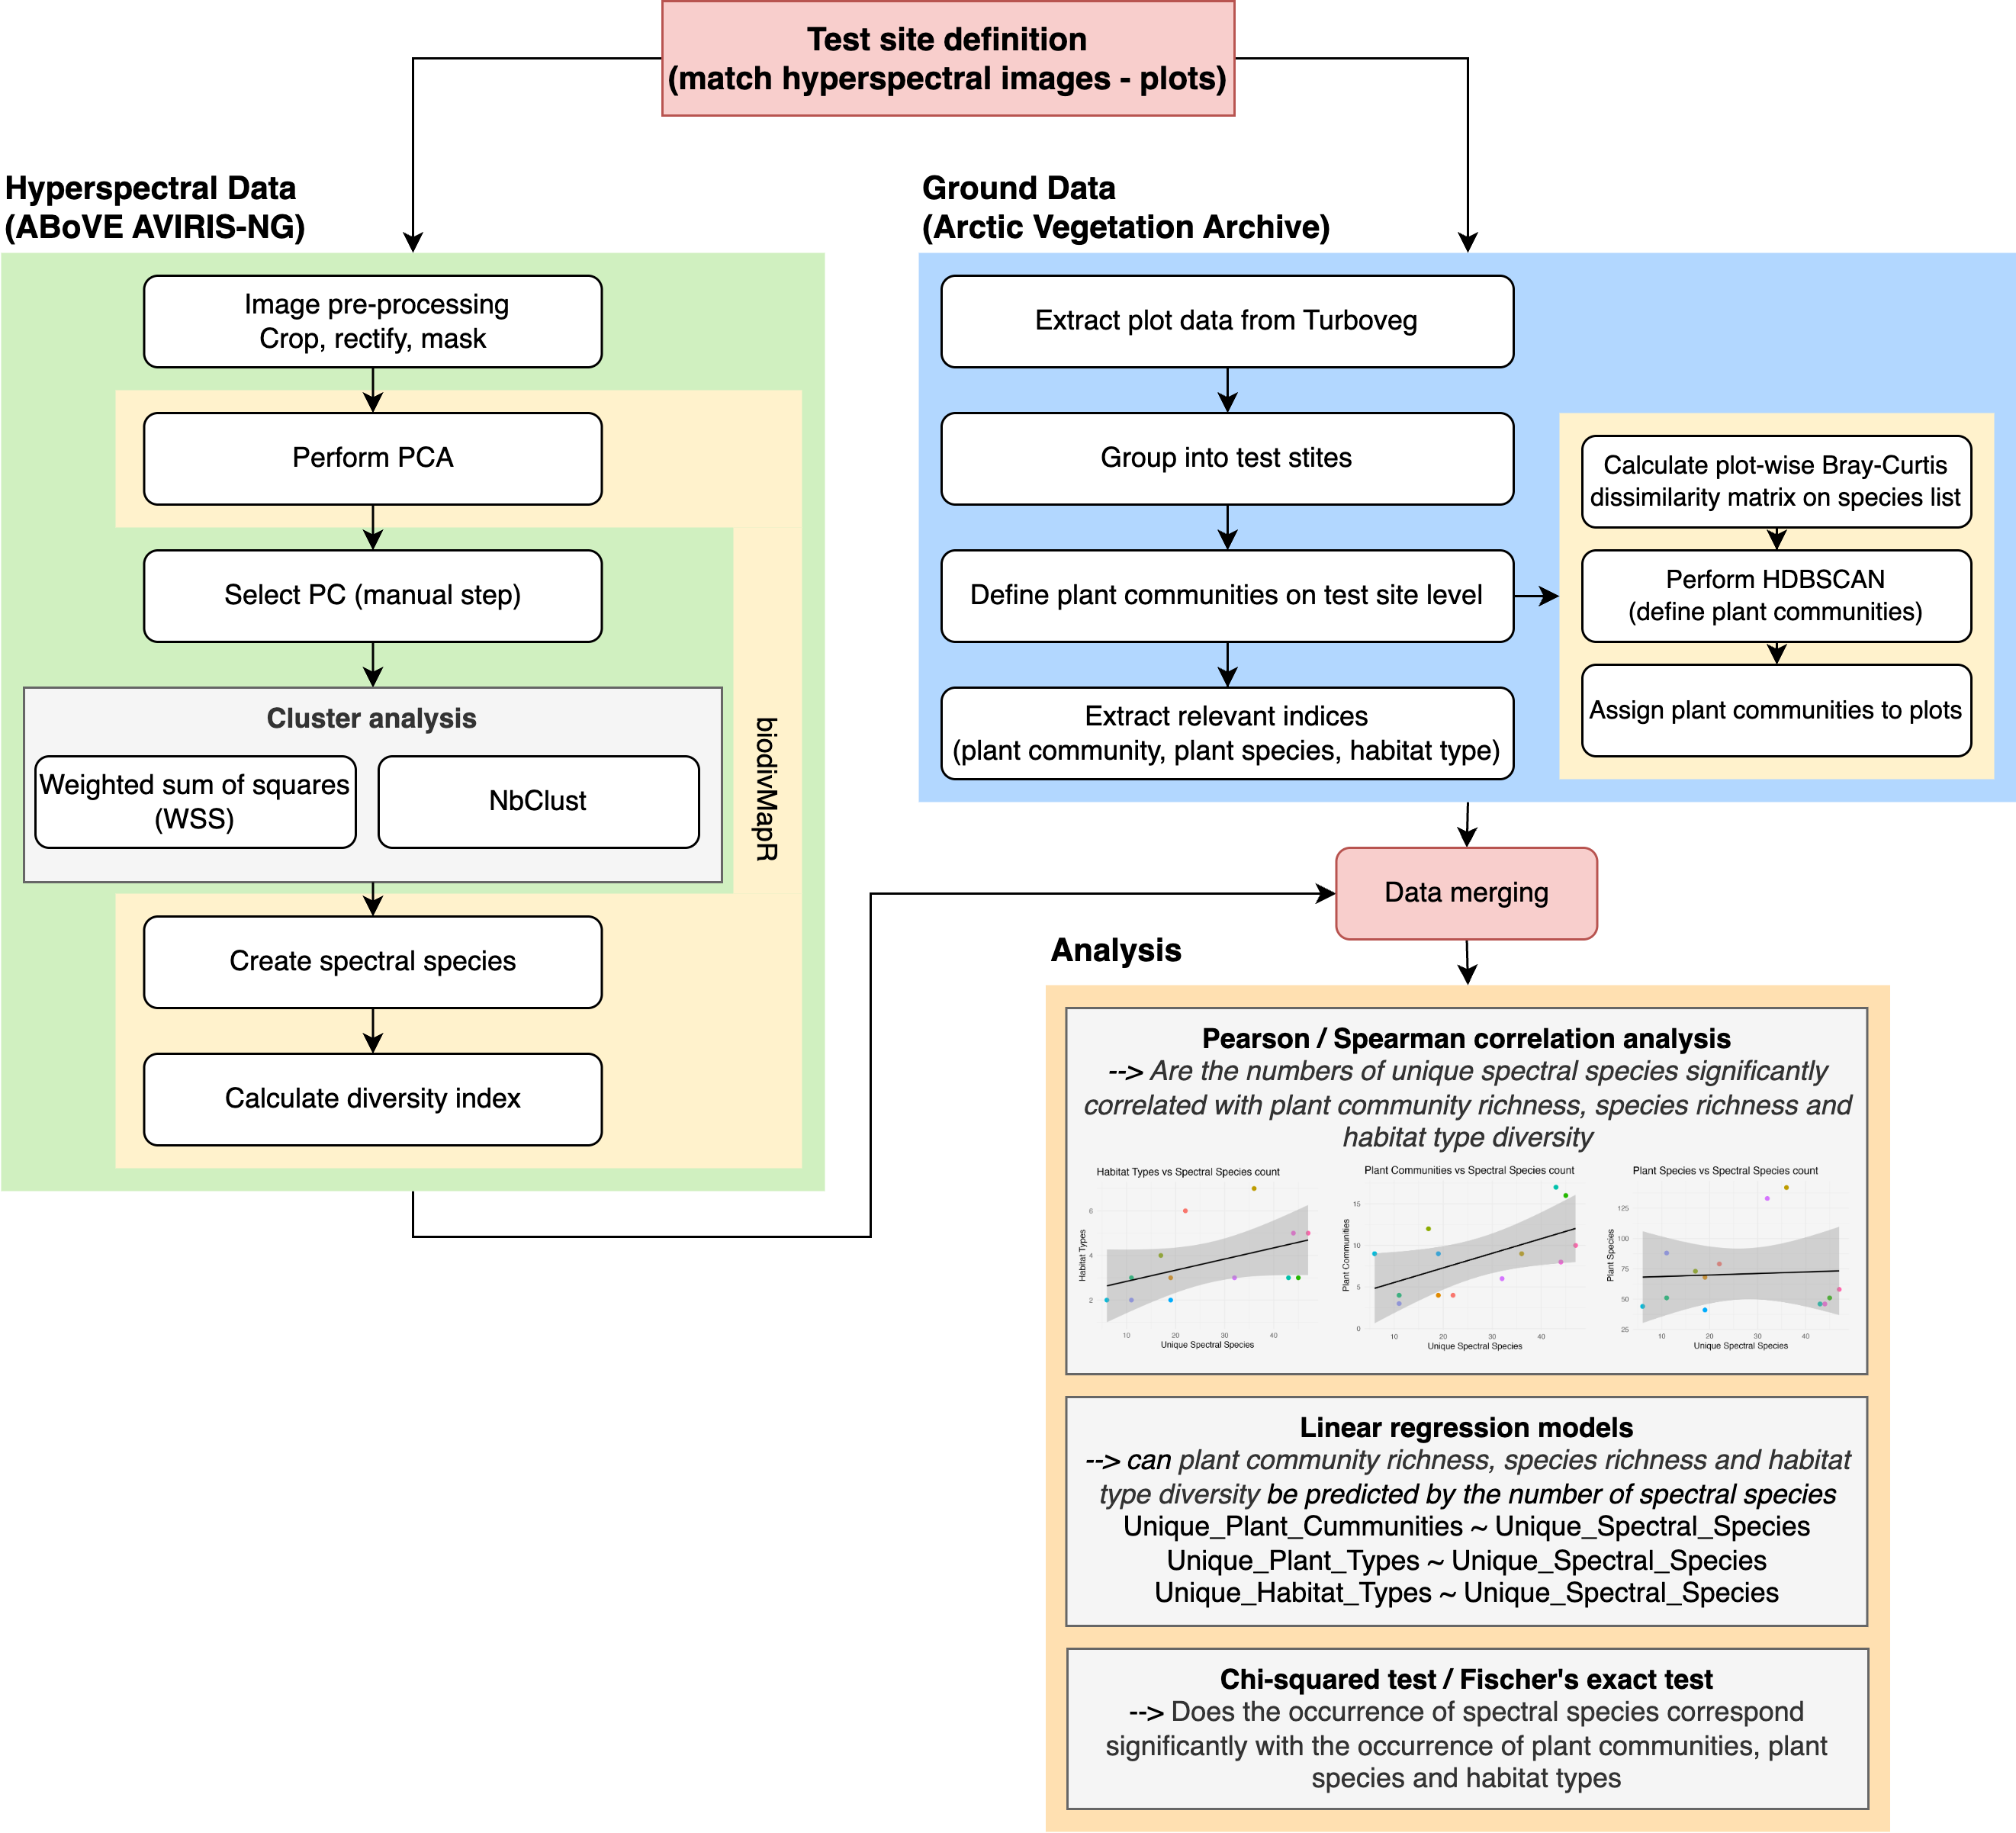
\includegraphics[width=0.9\textwidth]{Figures/WorkflowDiagram.png} % Replace with your actual image path
    \caption{Thesis workflow: This process flow diagram outlines the steps undertaken in both data streams, "Hyperspectral Data" and "Ground Data", to derive results from each. In the final stage, the outcome of the two streams are combined, allowing for statistical validation of the thesis hypothesis.}
    \label{fig:thesis_workflow}
\end{figure}

%----------------------------------------------------------------------------------------

\section{Test site definition}
To ensure the analysis included only hyperspectral imagery paired with corresponding in-situ data, I cross-referenced \ac{avirisng} flight lines with vegetation plot locations from the \ac{ava}. Further, only datasets from July and August were used, as these months presumably offer optimal vegetation coverage in the Arctic tundra. By overlaying spatial data, I identified 13 test sites, distributed across subzones C, D, and E of the northern Alaskan Arctic tundra as can be seen in Fig. \ref{fig:testsite_overview}. Additional metrics for the test sites can be seen Tab. \ref{tab:testsite_metadata}.
\begin{figure}[H]
    \centering
    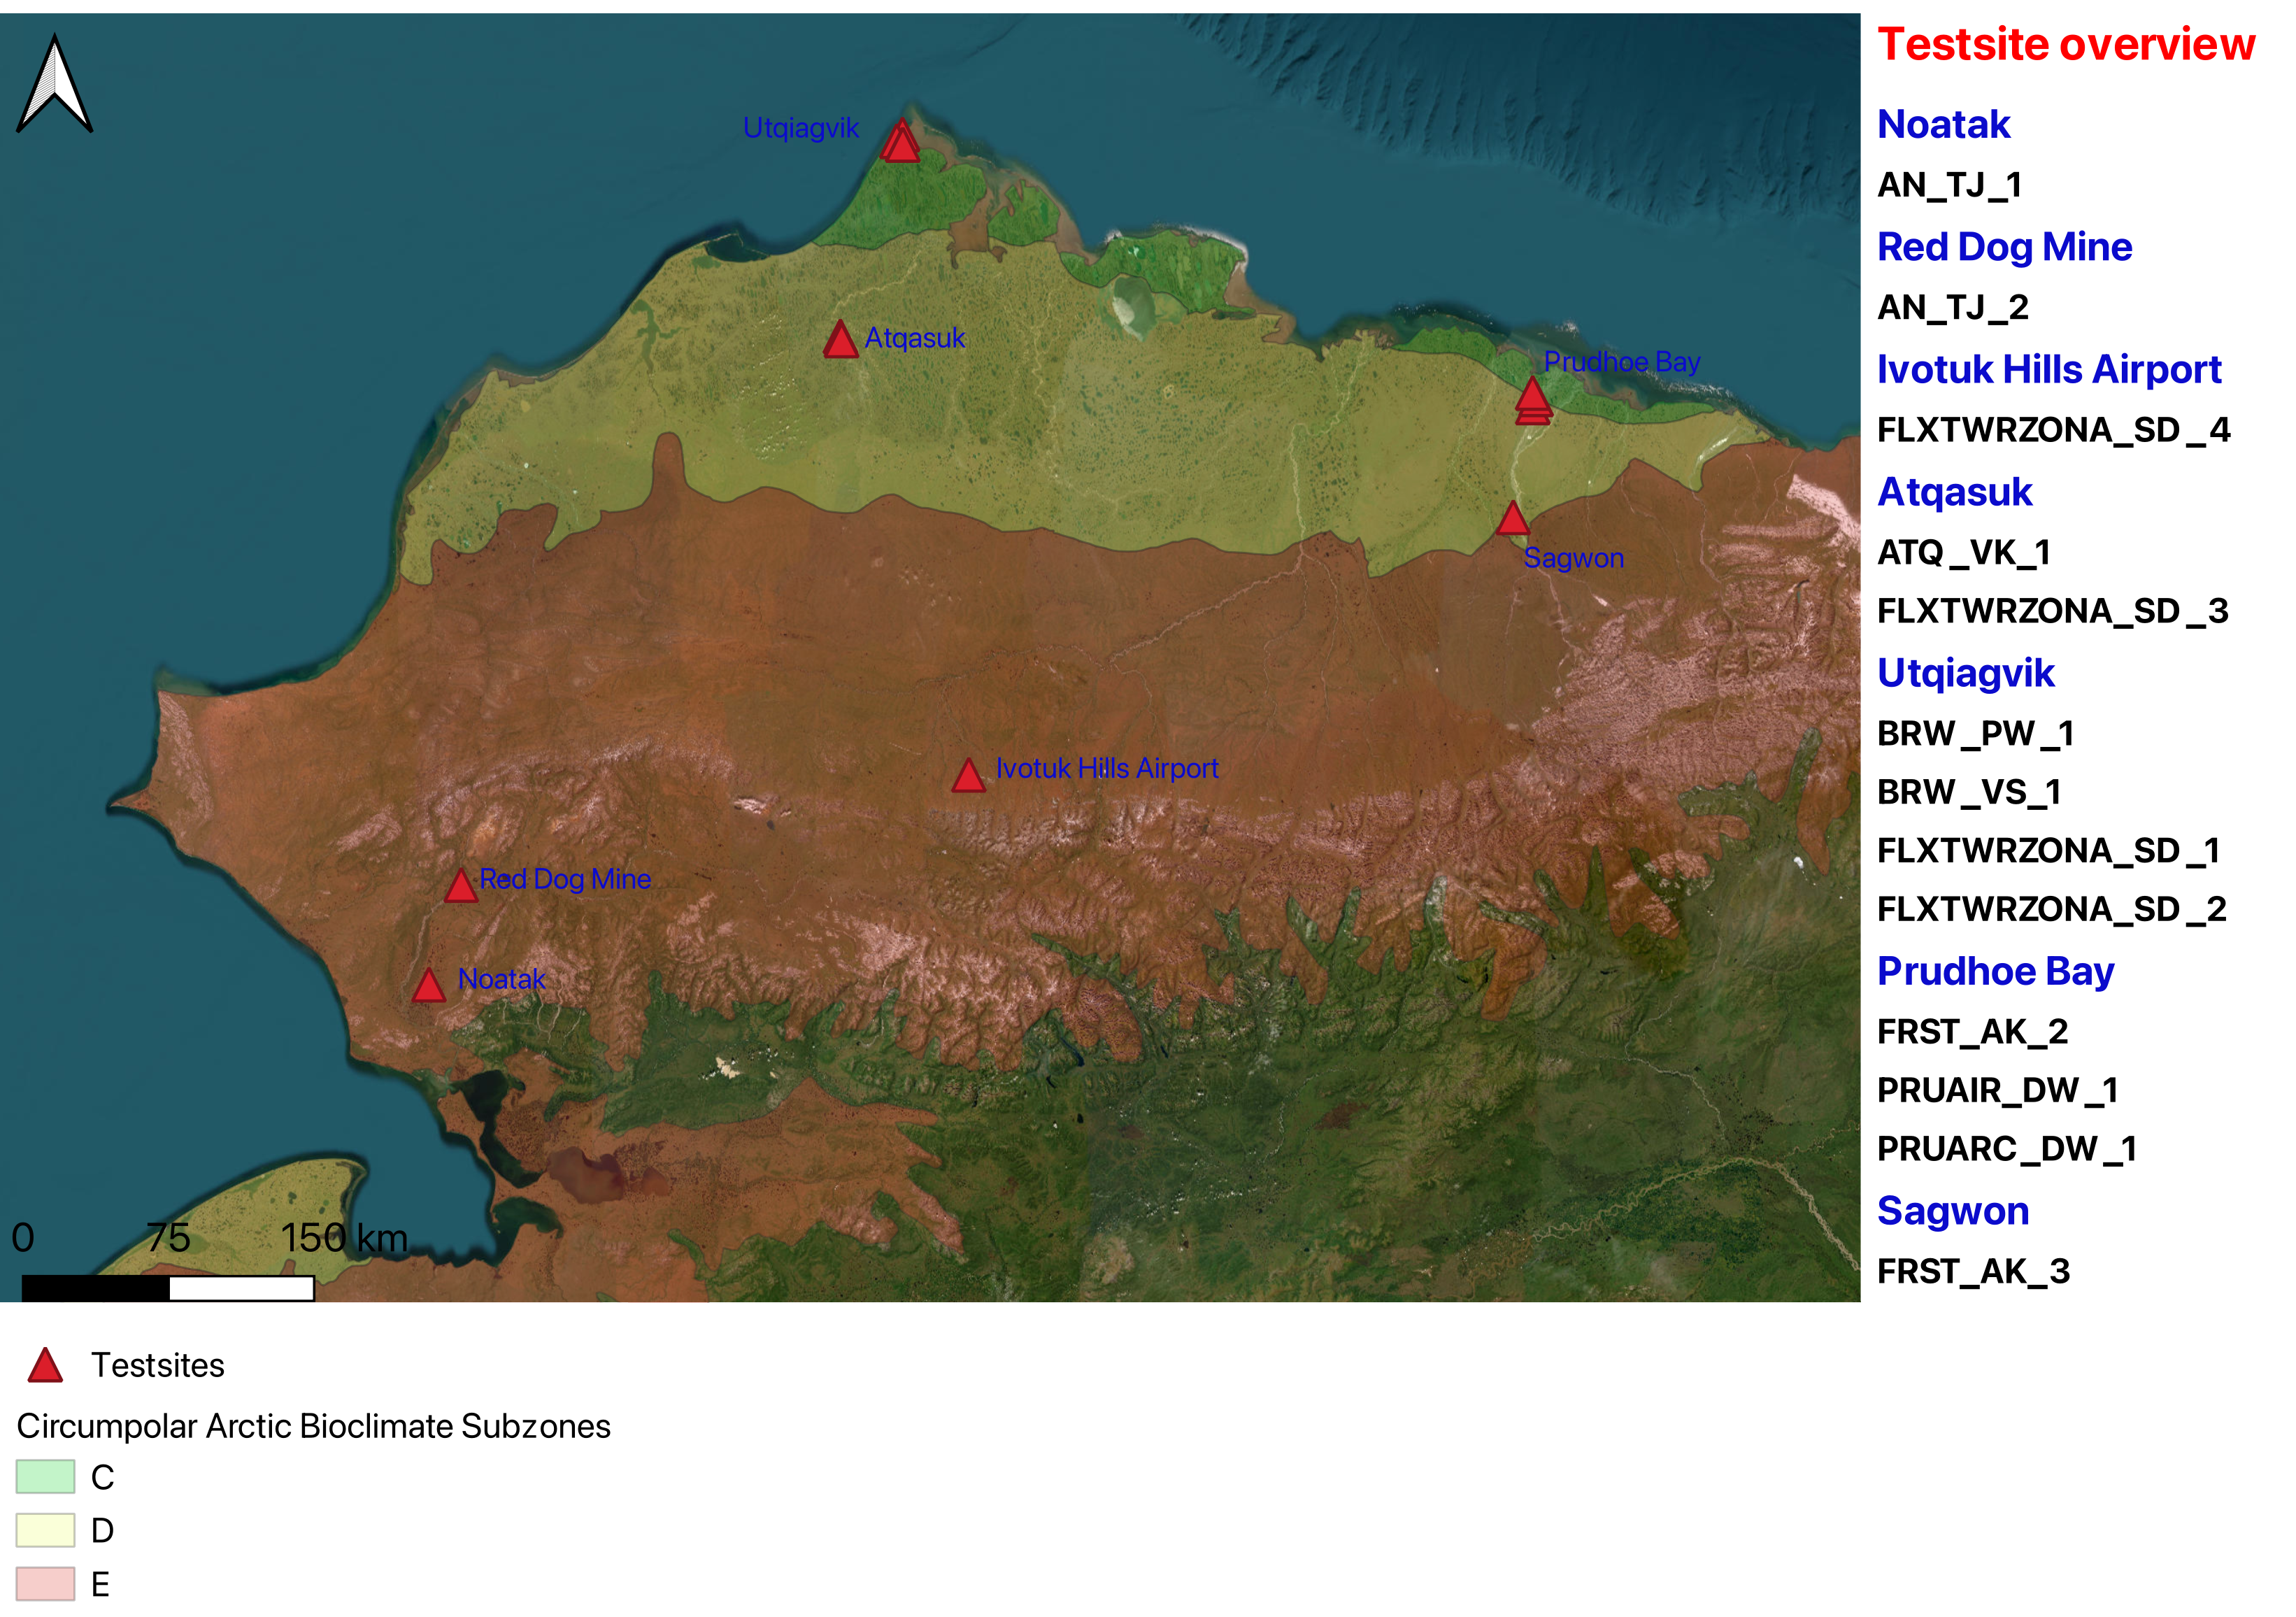
\includegraphics[width=0.9\textwidth]{Figures/TestSiteOverview.png} % Replace with your actual image path
    \caption{Map of the thirteen test sites across subzones C, D, and E of the northern Alaskan Arctic Tundra.}
    \label{fig:testsite_overview}
\end{figure}

\begin{table}[htbp]
\centering
\caption{Test sites with corresponding flight IDs, principal components retained, and site metadata. The hyperspectral images with the IDs ang20190712t231624 and ang20190712t212208 could be used for multiple test sites}
\resizebox{\textwidth}{!}{%
\begin{tabular}{lllllll}
\hline
\textbf{Test site} & \textbf{Flight ID} & \textbf{Year Flightstrip} & \textbf{Year Plots} & \textbf{Subzone} \\
\hline
AN\_TJ\_1 & \href{https://popo.jpl.nasa.gov/avng/y22/ang20220711t002111rfl.tar.gz}{ang20220711t002111}  & 2022 & 2005 & E \\
AN\_TJ\_2 & \href{https://popo.jpl.nasa.gov/avng/y22/ang20220711t003358rfl.tar.gz}{ang20220711t003358}  & 2022 & 2005 & E \\
ATQ\_VK\_1 & \href{https://popo.jpl.nasa.gov/avng/y19/ang20190712t231624rfl.tar.gz}{ang20190712t231624}  & 2019 & 2010 & D \\
BRW\_PW\_1 & \href{https://popo.jpl.nasa.gov/avng/y19/ang20190712t212208rfl.tar.gz}{ang20190712t212208}  & 2019 & 2010 & C \\
BRW\_VS\_1 & \href{https://popo.jpl.nasa.gov/avng/y19/ang20190712t212208rfl.tar.gz}{ang20190712t212208}  & 2019 & 2012 & C \\
FLXTWRZONA\_SD\_1 & \href{https://popo.jpl.nasa.gov/avng/y19/ang20190712t211646rfl.tar.gz}{ang20190712t211646}  & 2019 & 2014 & C \\
FLXTWRZONA\_SD\_2 & \href{https://popo.jpl.nasa.gov/avng/y19/ang20190712t212208rfl.tar.gz}{ang20190712t212208}  & 2019 & 2014 & C \\
FLXTWRZONA\_SD\_3 & \href{https://popo.jpl.nasa.gov/avng/y19/ang20190712t231624rfl.tar.gz}{ang20190712t231624}  & 2019 & 2014 & D \\
FLXTWRZONA\_SD\_4 & \href{https://popo.jpl.nasa.gov/avng/y19/ang20190706t210739rfl.tar.gz}{ang20190706t210739}  & 2019 & 2014 & E \\
FRST\_AK\_2 & \href{https://popo.jpl.nasa.gov/avng/y22/ang20220709t233937rfl.tar.gz}{ang20220709t233937}  & 2022 & 2001 & D \\
FRST\_AK\_3 & \href{https://popo.jpl.nasa.gov/avng/y19/ang20190713t024201rfl.tar.gz}{ang20190713t024201}  & 2019 & 2001 & D \\
PRUAIR\_DW\_1 & \href{https://popo.jpl.nasa.gov/avng/y17/ang20170709t003728rfl.tar.gz}{ang20170709t003728}  & 2017 & 2015 & C \\
PRUARC\_DW\_1 & \href{https://popo.jpl.nasa.gov/avng/y17/ang20170709t000442rfl.tar.gz}{ang20170709t000442}  & 2017 & 2014 & C \\
\hline
\end{tabular}
}
\label{tab:testsite_metadata}
\end{table}


\section{In-Situ data workflow}
Habitat type and species information were directly extracted from the Turboveg datasets, as these use standardized nomenclature. In contrast, plant community names lacked standardization and were assigned using two different classification systems: the Braun-Blanquet method and the Field Community Name method. This introduced a high degree of subjectivity from field observers. As a result, the combined dataset from all test sites contained 354 plot locations and 64 distinct plant community names. To address this inconsistency, I reclassified plant communities on the test site level using an unsupervised clustering approach. I applied \ac{hdbscan} (\cite{noauthor_how_nodate}) to the first two principal coordinates from a Bray-Curtis dissimilarity matrix based on species abundance data. Principal coordinates were extracted via \ac{pcoa} using the \fun{cmdscale} function. \ac{hdbscan} was run with a minimum points threshold of 2 to detect dense clusters while minimizing noise. Each plot was assigned a cluster ID representing a plant community, resulting in the numbers shown in Tab. \ref{tab:unique_features}, column "Unique plant communities". The result plots for each test site can be found in Appendix \ref{Appendix_PlantCommunityClustering}

\begin{table}[htbp]
\centering
\caption{Summary of unique biological and spectral features observed at each test site.}
\resizebox{\textwidth}{!}{%
\begin{tabular}{lccccc}
\hline
\textbf{Test site} & \textbf{Unique plant communities} & \textbf{Unique habitat types} & \textbf{Unique plant species} & \textbf{Unique spectral species} \\
\hline
\texttt{AN\_TJ\_1} & 4 & 6 & 79 & 26 \\
\texttt{AN\_TJ\_2} & 4 & 3 & 68 & 12 \\
\texttt{ATQ\_VK\_1} & 9 & 7 & 142 & 43 \\
\texttt{BRW\_PW\_1} & 12 & 4 & 73 & 40 \\
\texttt{BRW\_VS\_1} & 16 & 3 & 51 & 25 \\
\texttt{FLXTWRZONA\_SD\_1} & 4 & 3 & 51 & 27 \\
\texttt{FLXTWRZONA\_SD\_2} & 17 & 3 & 46 & 11 \\
\texttt{FLXTWRZONA\_SD\_3} & 9 & 2 & 44 & 27 \\
\texttt{FLXTWRZONA\_SD\_4} & 9 & 2 & 41 & 7 \\
\texttt{FRST\_AK\_2} & 3 & 2 & 88 & 48 \\
\texttt{FRST\_AK\_3} & 6 & 3 & 133 & 5 \\
\texttt{PRUAIR\_DW\_1} & 8 & 5 & 46 & 7 \\
\texttt{PRUARC\_DW\_1} & 10 & 5 & 58 & 42 \\
\hline
\end{tabular}
}
\label{tab:unique_features}
\end{table}



\section{Hyperspectral data workflow}
To derive biodiversity metrics from hyperspectral imagery, I implemented a multi-step processing workflow. This included image pre-processing, dimensionality reduction, cluster analysis, and the generation of spectral species and diversity index maps. Each step is described in the following sub-chapters.

\subsection{Image pre-processing}
I downloaded the specific \ac{avirisng} hyperspectral images corresponding to the selected test sites as seen in Tab. \ref{tab:testsite_metadata} in the ENVI file format from Earthdata Search ({\small\url{https://search.earthdata.nasa.gov/}}). For each test site, I generated a rectangular bounding box that encompassed all in-situ plot locations, including a 20 meter buffer to ensure full coverage while minimizing computational costs. The downloaded images were subsequently cropped to the extent of these bounding boxes. The biodivMapR package relies on underlying R packages that do not support "rotated" images. Therefore, I geometrically rectified the images to ensure compatibility. Geometric rectification and cropping were performed using the gdalwarp tool from \ac{gdal} with the following parameters: \param{-cutline} to define the bounding box boundary, \param{-crop\_to\_cutline} to limit the output to this extent, \param{-of ENVI} to specify the output format, \param{-co INTERLEAVE=BIL} to set the band interleave format, and \param{-dstnodata} \val{-9999} to assign a no-data value. To isolate vegetated areas within the hyperspectral imagery, a \ac{savi}  mask was generated, using Eq. \ref{eq:savi}.

\begin{equation}
\text{SAVI} = \frac{(NIR - Red) \times (1 + L)}{NIR + Red + L}
\label{eq:savi}
\end{equation}

The masking process utilized the \ac{nir} and Red spectral bands along with a soil brightness correction factor ($L$). Specifically, the \ac{nir} band was calculated by averaging wavelengths from 802 nm to 898 nm, and the Red band from 652 nm to 697 nm. I chose an $L$-value of 0.5, as it is generally appropriate for a wide range of land cover types. (\cite{noauthor_landsat_nodate}). Pixels exhibiting a \ac{savi} value greater than 0.2 were subsequently classified as vegetated and all other pixels classified as non-vegetated.

\subsection{\ac{pca}}
\ac{pca} (\cite{wold_principal_1987}) was conducted using the \fun{perform\_PCA} function from the biodivMapR package. Sparse \ac{pca} (sPCA) was chosen as the specific \ac{pca} type due to its suitability for high-dimensional hyperspectral data, allowing for noise reduction (\cite{feret_mapping_2014}; \cite{feret_biodivmapr_2020}; \cite{li_dimensionality_2022}; \cite{ruiz_hidalgo_dimensionality_2021}). During the analysis, the following biodivMapR parameters were applied: \param{Continuum\_Removal} was set to \val{FALSE}, the \param{TypePCA} was specified as \val{SPCA}, \param{NbPCs\_To\_Keep} was set to \val{30}, \param{FilterPCA} was set to \val{FALSE} and \param{nb\_partitions} was set to \val{20}.

\subsection{PC selection}
Following the \ac{pca}, 30 principal components (PCs) were retained for every test site for subsequent steps. The developers of the biodivMapR package indicate that some PCs, despite explaining only a small portion of the total variance, can still capture valuable information related to plant diversity. To account for this and ensure the inclusion of relevant components, a visual assessment of the principal component images was recommended by the authors. Given the large number of test sites, each PC image was saved as 30 separate \ac{png} files to facilitate this visual inspection and selection process.

\subsection{Cluster analysis}
To generate spectral species, the biodivMapR package employs k-means clustering on the retained principal components. This clustering algorithm requires a predefined number of clusters (k). While many studies have opted for a fixed number of clusters across their analyses (\cite{feret_mapping_2014}; \cite{pijnenburg_mapping_2023}; \cite{zhang_assessment_2023}; \cite{robertson_effects_2023}; \cite{liccari_use_2022}), this research takes a data-driven approach. For each image, the optimal number of clusters is estimated using the Elbow Method (\cite{thorndike_who_1953}; \cite{fritz_log-means_2020}). I first removed rows with missing (NA) values and scaled the data. Then, I evaluated multiple values for the nstart parameter, which controls the number of random initial configurations, to identify the setting that produced the lowest \ac{wcss} for a fixed number of clusters. Since my tests showed that the Elbow Method is highly sensitive to the \param{nstart} value, determining the optimal setting was essential. Once identified, I assessed the \ac{wcss} across a range of cluster numbers (2 to 50). The "elbow" point, representing the optimal number of clusters, was determined by analyzing the second derivative of the \ac{wcss} curve, marking the point where the rate of decrease in \ac{wcss} noticeably slowed. Additionally, I explored a second method for estimating the optimal number of clusters using the NbClust R package. This approach tested 15 clustering indices considered suitable for PCA-processed hyperspectral data. Although I did not use these results in the subsequent analysis, they underscored the substantial variability in optimal cluster estimates depending on the chosen method.

\subsection{Spectral Species and Diversity Indices}
Spectral species maps were generated using the \fun{map\_spectral\_species} function from the biodivMapR package, with the optimal number of clusters for each image set via the \param{nbclusters} parameter. Based on these spectral species, Shannon and Simpson diversity indices were computed using \fun{map\_alpha\_div}, while beta diversity was mapped using \fun{map\_beta\_div} with \param{TypePCA} set to \val{SPCA} and \param{scaling} applied using principal coordinate analysis (\val{PCO}). For all diversity maps, \param{nbclusters} was set to the previously determined cluster count, and a \param{window\_size} of \val{5} (corresponding to a 5x5 pixel or 25x25 meter window) was used to define the local neighborhood for analysis.

\section{Data analysis}
The following subsections describe the types of analyses conducted. I examined the correlations both across all test sites collectively and within spatially defined groups. Specifically, test sites in subzones C and D were grouped together due to their close alignment along the same latitude, while subzone E was analyzed separately. Tab. \ref{tab:testsite_grouped} presents the group definitions along with the corresponding test sites included in each group.

\begin{table}[htbp]
\centering
\caption{Grouping of All Sites into Group C/D and Group E}
\resizebox{\textwidth}{!}{%
\begin{tabular}{|l|l|l|}
\hline
\textbf{All Test Sites} & \textbf{Group C/D} & \textbf{Group E} \\
\hline
AN\_TJ\_1               & -                  & AN\_TJ\_1         \\
AN\_TJ\_2               & -                  & AN\_TJ\_2         \\
ATQ\_VK\_1              & ATQ\_VK\_1         & -                 \\
BRW\_PW\_1              & BRW\_PW\_1         & -                 \\
BRW\_VS\_1              & BRW\_VS\_1         & -                 \\
FLXTWRZONA\_SD\_1       & FLXTWRZONA\_SD\_1  & -                 \\
FLXTWRZONA\_SD\_2       & FLXTWRZONA\_SD\_2  & -                 \\
FLXTWRZONA\_SD\_3       & FLXTWRZONA\_SD\_3  & -                 \\
FLXTWRZONA\_SD\_4       & -                  & FLXTWRZONA\_SD\_4 \\
FRST\_AK\_2             & FRST\_AK\_2        & -                 \\
FRST\_AK\_3             & FRST\_AK\_3        & -                 \\
PRUAIR\_DW\_1           & PRUAIR\_DW\_1      & -                 \\
PRUARC\_DW\_1           & PRUARC\_DW\_1      & -                 \\
\hline
\end{tabular}
}
\label{tab:testsite_grouped}
\end{table}


\subsection{Correlation analysis}
To investigate the relationships between spectral diversity and ecological diversity, I conducted a series of pairwise correlation analyses. Specifically, the number of unique spectral species, derived from remote sensing data, was compared against three key ecological indicators: the number of unique plant communities, the number of distinct habitat types, and the number of unique plant species recorded at each site.

Before performing the correlation tests, I assessed the distributions of each variable using the Shapiro-Wilk test to determine whether they conformed to a normal distribution. Based on these normality checks and the number of observations available, the most appropriate correlation method was selected for each comparison. Pearson’s correlation coefficient was applied when both variables were normally distributed and sample sizes were sufficient. For non-normally distributed data, Spearman’s rank correlation was used. In cases with fewer than ten observations, Kendall’s tau was chosen as a more appropriate non-parametric alternative.

The strength and direction of the correlations were visualized using scatter plots, generated with the ggplot2 package in R. These plots included linear trendlines with confidence intervals of 95\% to aid interpretation. Alongside the visualizations, the correlation coefficient (R), p-value, and a qualitative interpretation of correlation strength were computed and recorded. To facilitate interpretation of correlation strength, the correlation coefficient ($R$) was categorized into nine levels based on its value and direction. A custom function was used to assign the following labels: \emph{very strong positive} ($R \geq 0.9$), \emph{strong positive} ($0.7 \leq R < 0.9$), \emph{moderate positive} ($0.4 \leq R < 0.7$), \emph{weak positive} ($0.1 \leq R < 0.4$), \emph{negligible correlation} ($-0.1 < R < 0.1$), \emph{weak negative} ($-0.4 < R \leq -0.1$), \emph{moderate negative} ($-0.7 < R \leq -0.4$), \emph{strong negative} ($-0.9 < R \leq -0.7$), and \emph{very strong negative} ($R \leq -0.9$). These categories provided a standardized and interpretable framework for describing the strength and direction of observed relationships (\cite{schober_correlation_2018}).

\subsection{Regression analysis}
In addition to the correlation analysis, I used simple linear regression to explore whether spectral species richness could predict in-situ biodiversity metrics. I fitted separate models for each response variable, unique plant communities, habitat types, and plant species, using spectral species count as the predictor. All models were created using the lm() function in R. Model performance was assessed through residual diagnostic plots and summary statistics, which provided insights into the significance, direction, and strength of the relationships. As the residual plots revealed issues with model assumptions, the linear regression results were not incorporated into the primary thesis findings. However, they are available for reference in Appendix \ref{Appendix_LinearRegression}.

\subsection{Spectral curve analysis}
The previous analysis were based on \ac{pca}-processed images. To assess the correspondence between directly extracted reflectance curves and in-situ measurements, mean reflectance values were calculated within a 5-meter radius around each plot location. Plot coordinates were obtained from the \ac{ava} dataset for this purpose. Prior to analysis, several wavelength intervals were excluded due to high outliers and known contamination sources, such as atmospheric water vapor absorption bands and noisy edge regions. Specifically, reflectance values were set to \texttt{NA} for wavelengths between 0–442\,nm, 1329–1429\,nm, 1800–1980\,nm, and those greater than 2456\,nm. Reflectance curves were then visualized in two ways: first, grouped by habitat type and plant community at the individual test site level, and second, aggregated solely by habitat type across all test sites. This dual representation supports evaluation of both site-specific and cross-site spectral consistency.


\subsection{Spatial autocorrelation}
In this analysis, spatial autocorrelation was not explicitly examined, and as such, the results should be interpreted with that limitation in mind. Without assessing autocorrelation, there is a possibility that observed spatial patterns may be influenced by the inherent structure of the data rather than by independent ecological or environmental drivers. Consequently, any spatial inferences drawn from these results should be approached with caution, and future analyses may benefit from incorporating tests to evaluate spatial dependency more rigorously.
%----------------------------------------------------------------------------------------
% CHAPTER 3
%----------------------------------------------------------------------------------------
\chapter{Results} % Main chapter title
\label{Chapter3}

The results revealed negligible to very strong relationships between spectral species richness and ecological diversity metrics. The following sections present the results for each ecological metric, plant species richness, plant community richness, and habitat type richness, in relation to spectral species richness.

\section{Plant species - spectral species}

\subsection{Results over all test sites}
The Spearman correlation analysis over all test sites indicated a moderate positive correlation between spectral species richness and plant species richness, with a correlation coefficient of $R$ = 0.4 (Fig. \ref{fig:WCSS_correlation_plant_species}). However, the linear regression model did not show a statistically significant relationship (Tab. \ref{tab:lm_plantspecies_spectral}). The model explained only a small portion of the variance in plant species richness ($R^2$ = 0.064), and the predictor variable was not significant ($p$ = 0.404).

\begin{figure}[H]
    \centering
    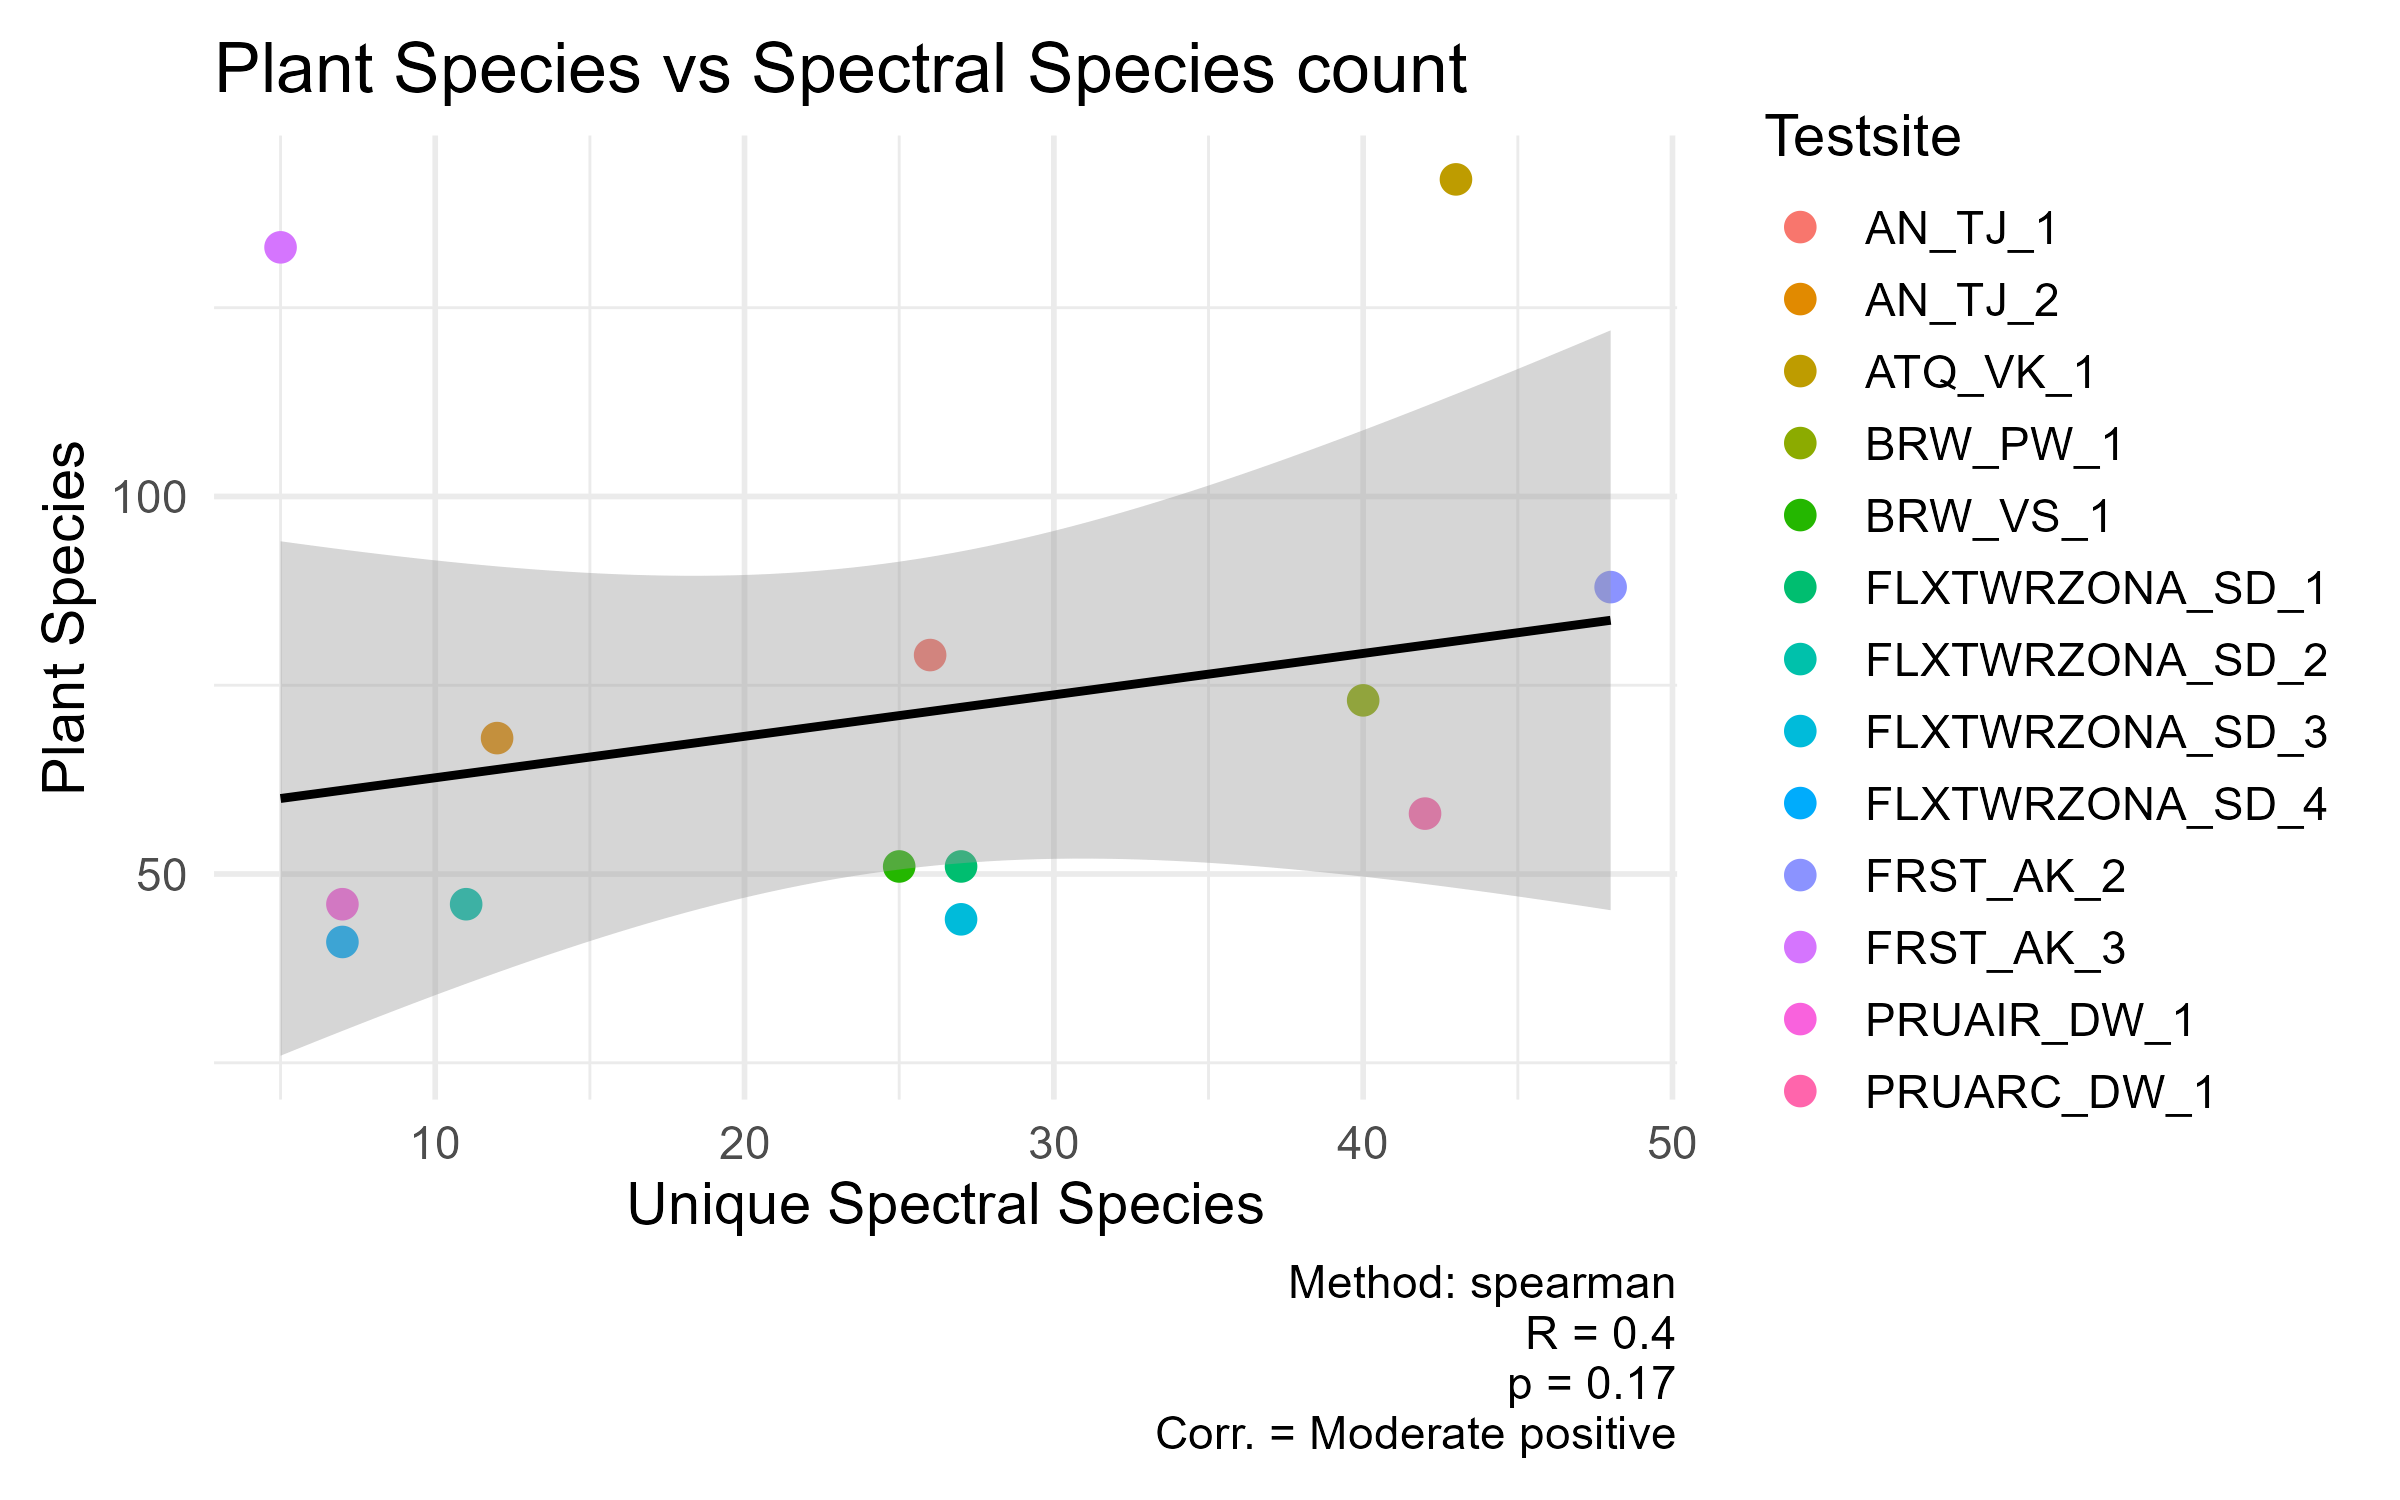
\includegraphics[width=0.9\textwidth]{Figures/WCSS_correlation_plant_species.png} % Replace with your actual image path
    \caption{The Spearman correlation test over all test sites shows a moderate positive correlation between spectral species and plant species with an $R$ value of 0.4 and a $p$-value of 0.17.}
    \label{fig:WCSS_correlation_plant_species}
\end{figure}

\begin{table}[ht]
\centering
\caption{Summary of linear regression model predicting plant species richness from spectral species richness over all test sites}
\begin{tabular}{lcccc}
\hline
\textbf{Predictor} & \textbf{Estimate} & \textbf{Std. Error} & \textbf{t value} & \textbf{Pr($>$$|$t$|$)} \\
\hline
Intercept & 57.2577 & 18.1108 & 3.162 & \textbf{0.00905**} \\
Unique Spectral Species & 0.5489 & 0.6323 & 0.868 & 0.40390 \\
\hline
\multicolumn{5}{l}{\textit{Residual standard error:} 33.38 on 11 degrees of freedom} \\
\multicolumn{5}{l}{\textit{Multiple R-squared:} 0.06411 \quad \textit{Adjusted R-squared:} -0.02097} \\
\multicolumn{5}{l}{\textit{F-statistic:} 0.7535 on 1 and 11 DF, \quad \textit{p-value:} 0.4039} \\
\hline
\end{tabular}
\label{tab:lm_plantspecies_spectral}
\end{table}

\subsection{Results for Group C/D}
The Spearman correlation analysis for Group C/D indicated a moderate positive correlation between spectral species richness and plant species richness, with a correlation coefficient of $R$ = 0.42 (Fig. \ref{fig:WCSS_correlation_plant_species_part_c_d}). However, the linear regression model did not show a statistically significant relationship (Tab. \ref{tab:lm_plantspecies_spectral_group_cd}). The model explained only a small portion of the variance in plant species richness ($R^2$ = 0.02931), and the predictor variable was not significant ($p$ = 0.636).
\begin{figure}[H]
    \centering
    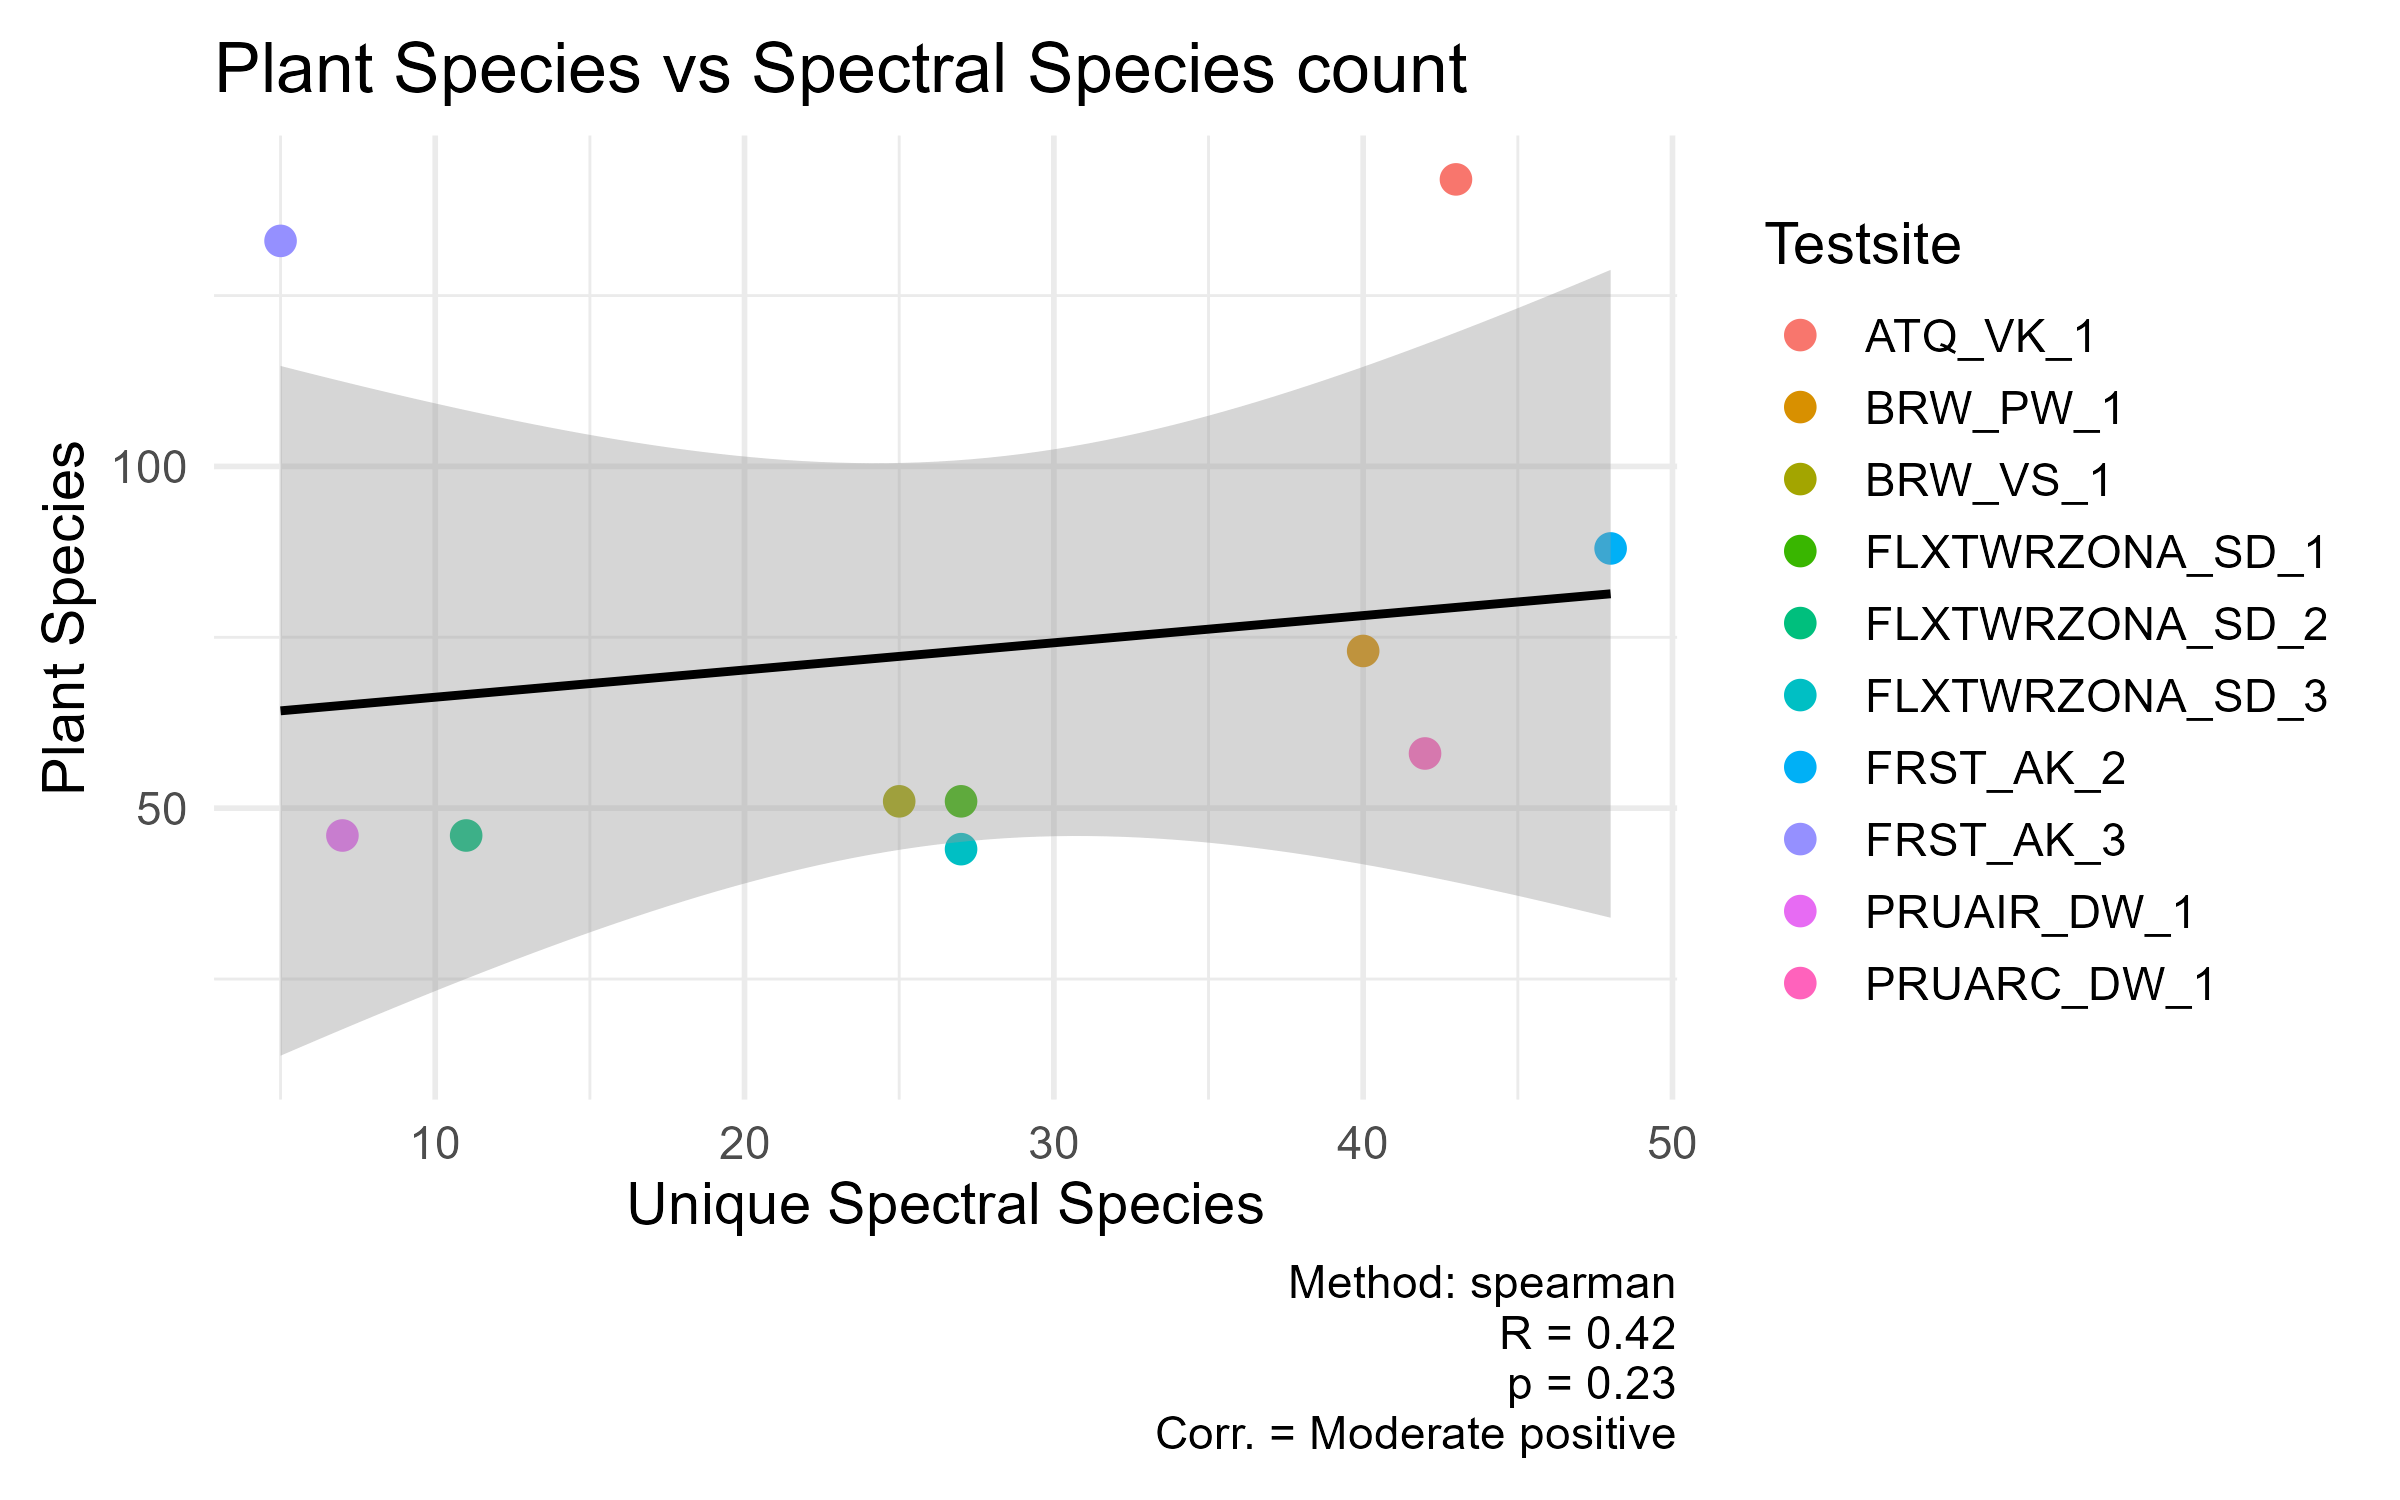
\includegraphics[width=0.9\textwidth]{Figures/WCSS_correlation_plant_species_part_c_d.png} % Replace with your actual image path
    \caption{The Spearman correlation test within Group C/D shows a moderate positive correlation between spectral species and plant species with an $R$ value of 0.42 and a $p$-value of 0.23.}
    \label{fig:WCSS_correlation_plant_species_part_c_d}
\end{figure}

\begin{table}[ht]
\centering
\caption{Summary of linear regression model predicting plant species richness from spectral species richness for Group C/D}
\begin{tabular}{lcccc}
\hline
\textbf{Predictor} & \textbf{Estimate} & \textbf{Std. Error} & \textbf{t value} & \textbf{Pr($>$$|$t$|$)} \\
\hline
Intercept & 62.2493 & 25.3566 & 2.455 & \textbf{0.0396*} \\
Unique Spectral Species & 0.3982 & 0.8102 & 0.491 & 0.6363 \\
\hline
\multicolumn{5}{l}{\textit{Residual standard error:} 38.28 on 8 degrees of freedom} \\
\multicolumn{5}{l}{\textit{Multiple R-squared:} 0.02931 \quad \textit{Adjusted R-squared:} -0.09203} \\
\multicolumn{5}{l}{\textit{F-statistic:} 0.2416 on 1 and 8 DF, \quad \textit{p-value:} 0.6363} \\
\hline
\end{tabular}
\label{tab:lm_plantspecies_spectral_group_cd}
\end{table}

\subsection{Results for Group E}
The Kendall’s tau correlation analysis for Group E indicated a very strong positive correlation between spectral species richness and plant species richness, with a correlation coefficient of $R$ = 1 (Fig. \ref{fig:WCSS_correlation_plant_species_part_e}). However, the linear regression model did not show a statistically significant relationship (Tab. \ref{tab:lm_plantspecies_spectral_group_e}). The model explained only a small portion of the variance in plant species richness ($R^2$ = 0.7656), and the predictor variable was not significant ($p$ = 0.636).
\begin{figure}[H]
    \centering
    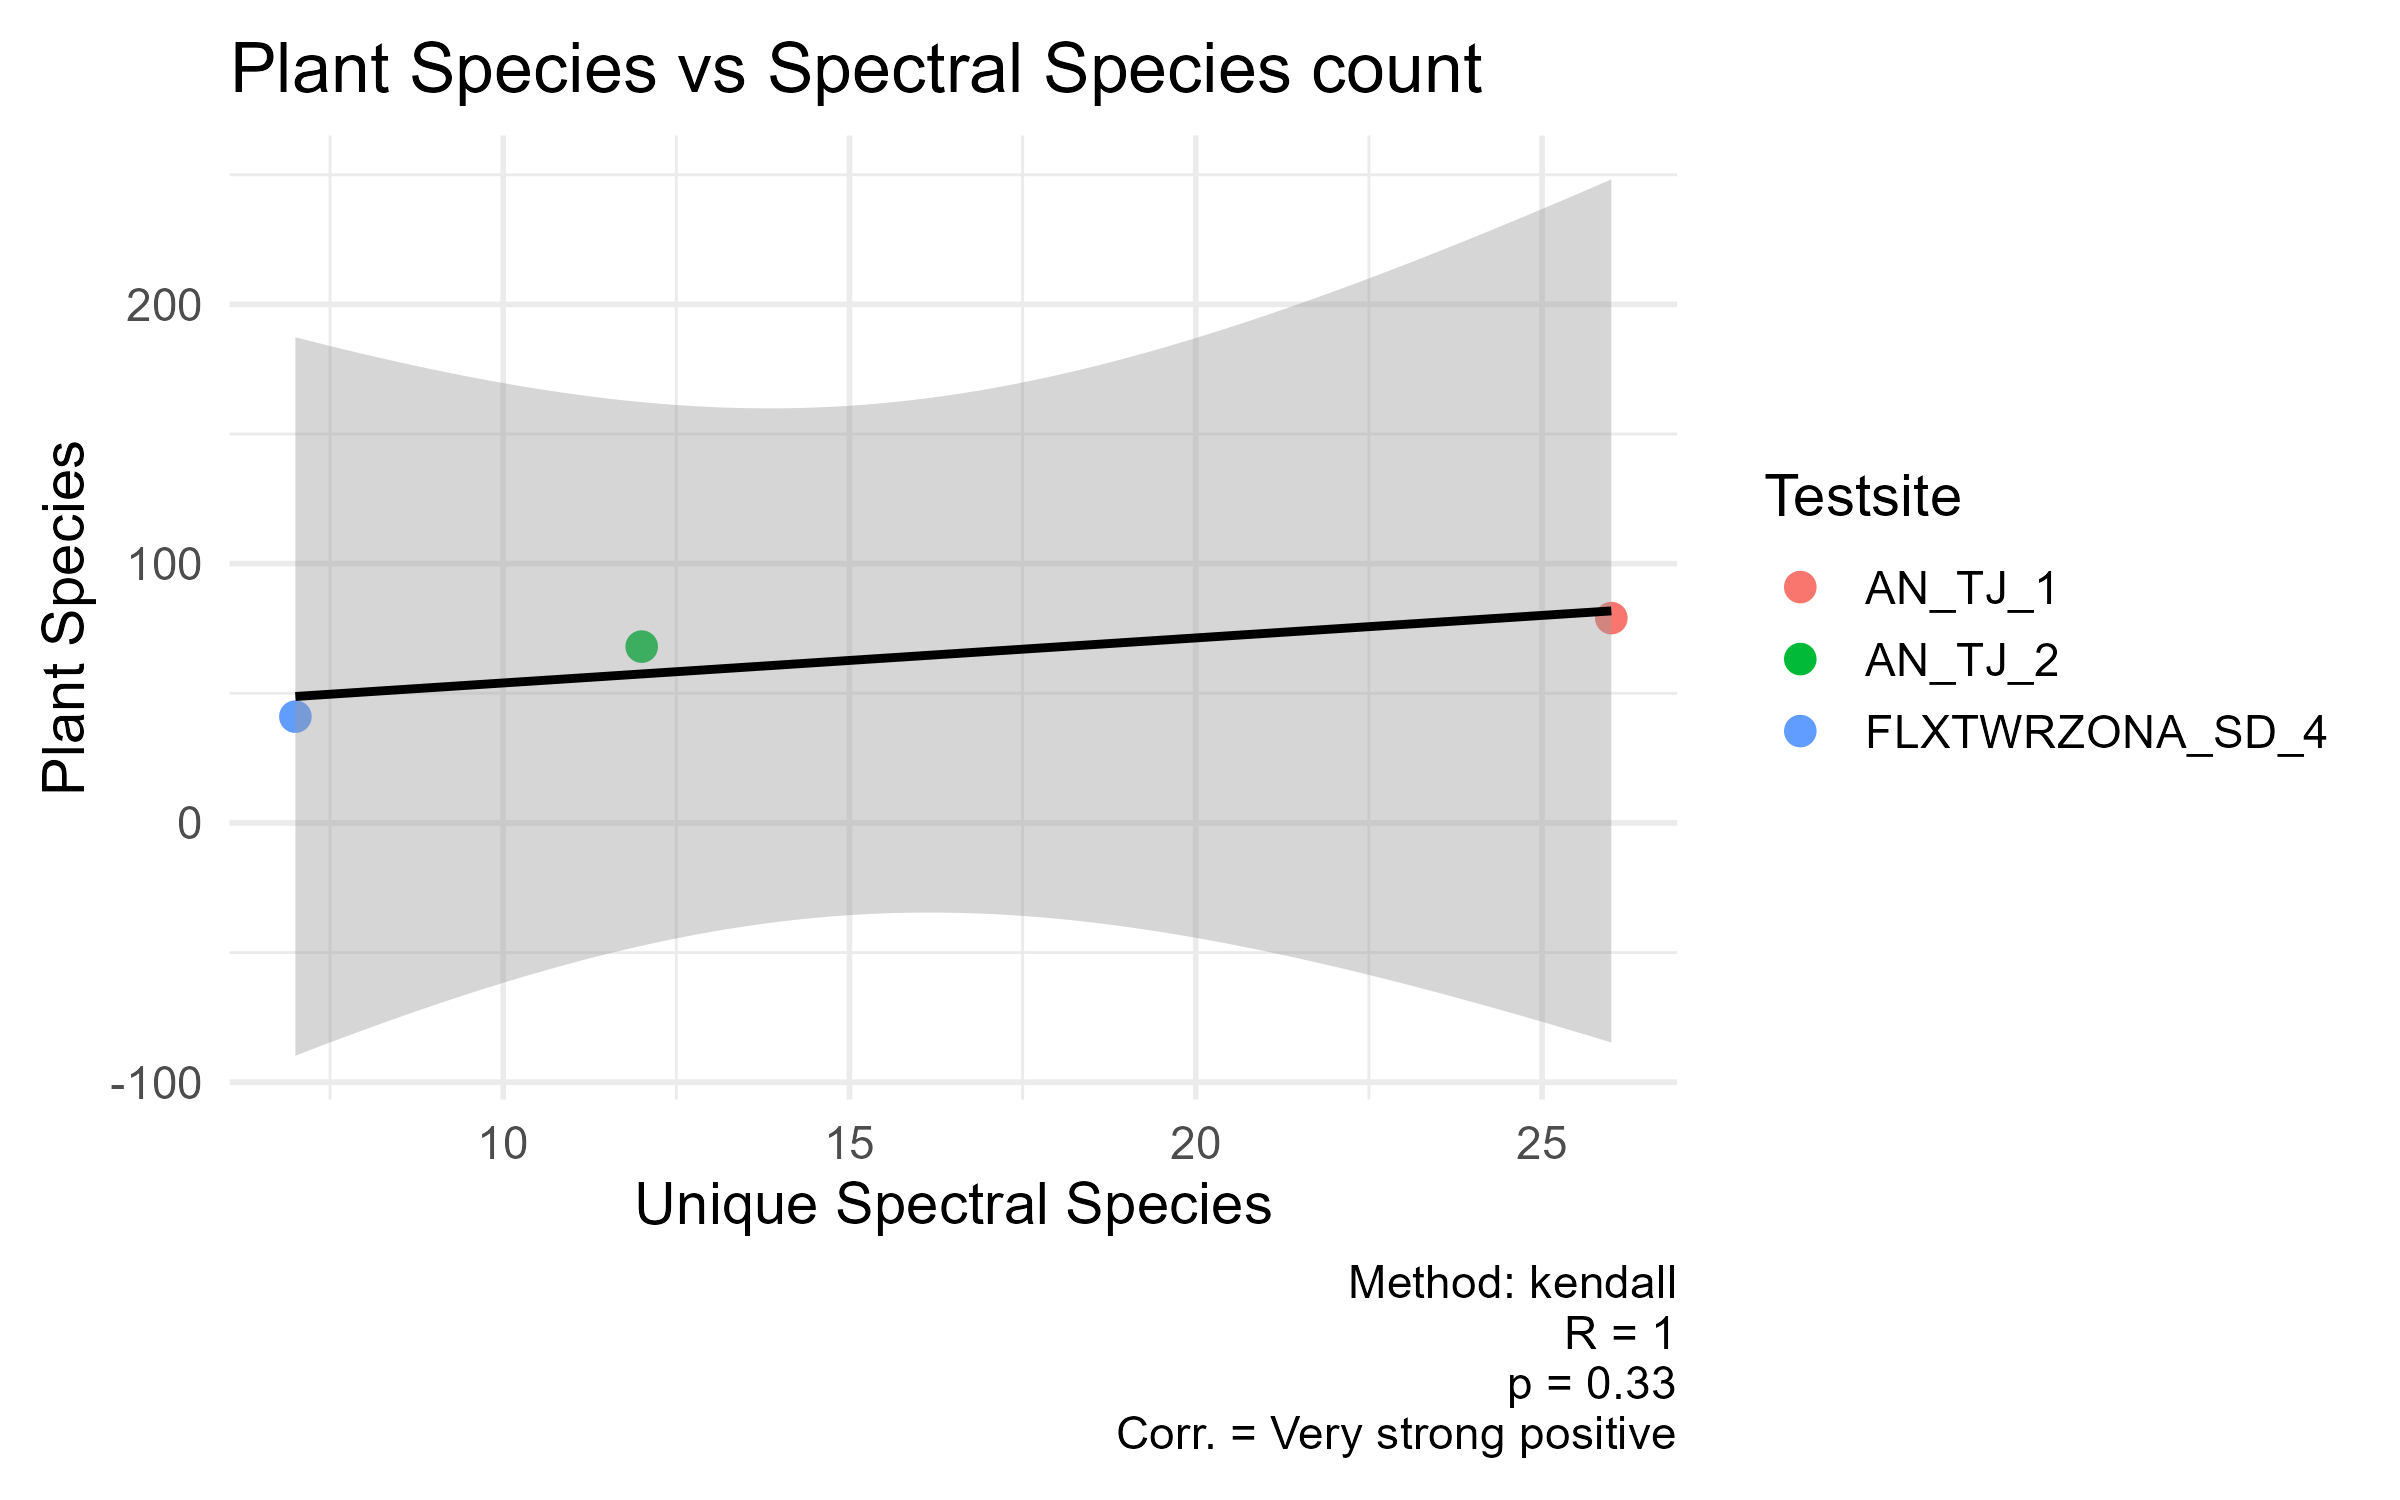
\includegraphics[width=0.9\textwidth]{Figures/WCSS_correlation_plant_species_part_e.png} % Replace with your actual image path
    \caption{The Kendall’s tau correlation test within Group E shows a very strong positive correlation between spectral species and plant species with an $R$ value of 1 and a $p$-value of 0.33.}
    \label{fig:WCSS_correlation_plant_species_part_e}
\end{figure}

\begin{table}[ht]
\centering
\caption{Summary of linear regression model predicting plant species richness from spectral species richness for Group E}
\begin{tabular}{lcccc}
\hline
\textbf{Predictor} & \textbf{Estimate} & \textbf{Std. Error} & \textbf{t value} & \textbf{Pr($>$$|$t$|$)} \\
\hline
Intercept & 36.6100 & 16.3602 & 2.238 &  0.268 \\
Unique Spectral Species & 1.7371 & 0.9613 & 1.807 & 0.322 \\
\hline
\multicolumn{5}{l}{\textit{Residual standard error:} 13.39 on 1 degrees of freedom} \\
\multicolumn{5}{l}{\textit{Multiple R-squared:} 0.7656 \quad \textit{Adjusted R-squared:} 0.5311} \\
\multicolumn{5}{l}{\textit{F-statistic:} 3.266 on 1 and 1 DF, \quad \textit{p-value:} 0.3218} \\
\hline
\end{tabular}
\label{tab:lm_plantspecies_spectral_group_e}
\end{table}


\section{Plant communities - spectral species}
\subsection{Results over all test sites}
The Pearson correlation analysis over all test sites indicated a negligible correlation between spectral species richness and plant community richness, with a correlation coefficient of $R$ = -0.08 (Fig. \ref{fig:WCSS_correlation_plant_communities}).

\begin{figure}[H]
    \centering
    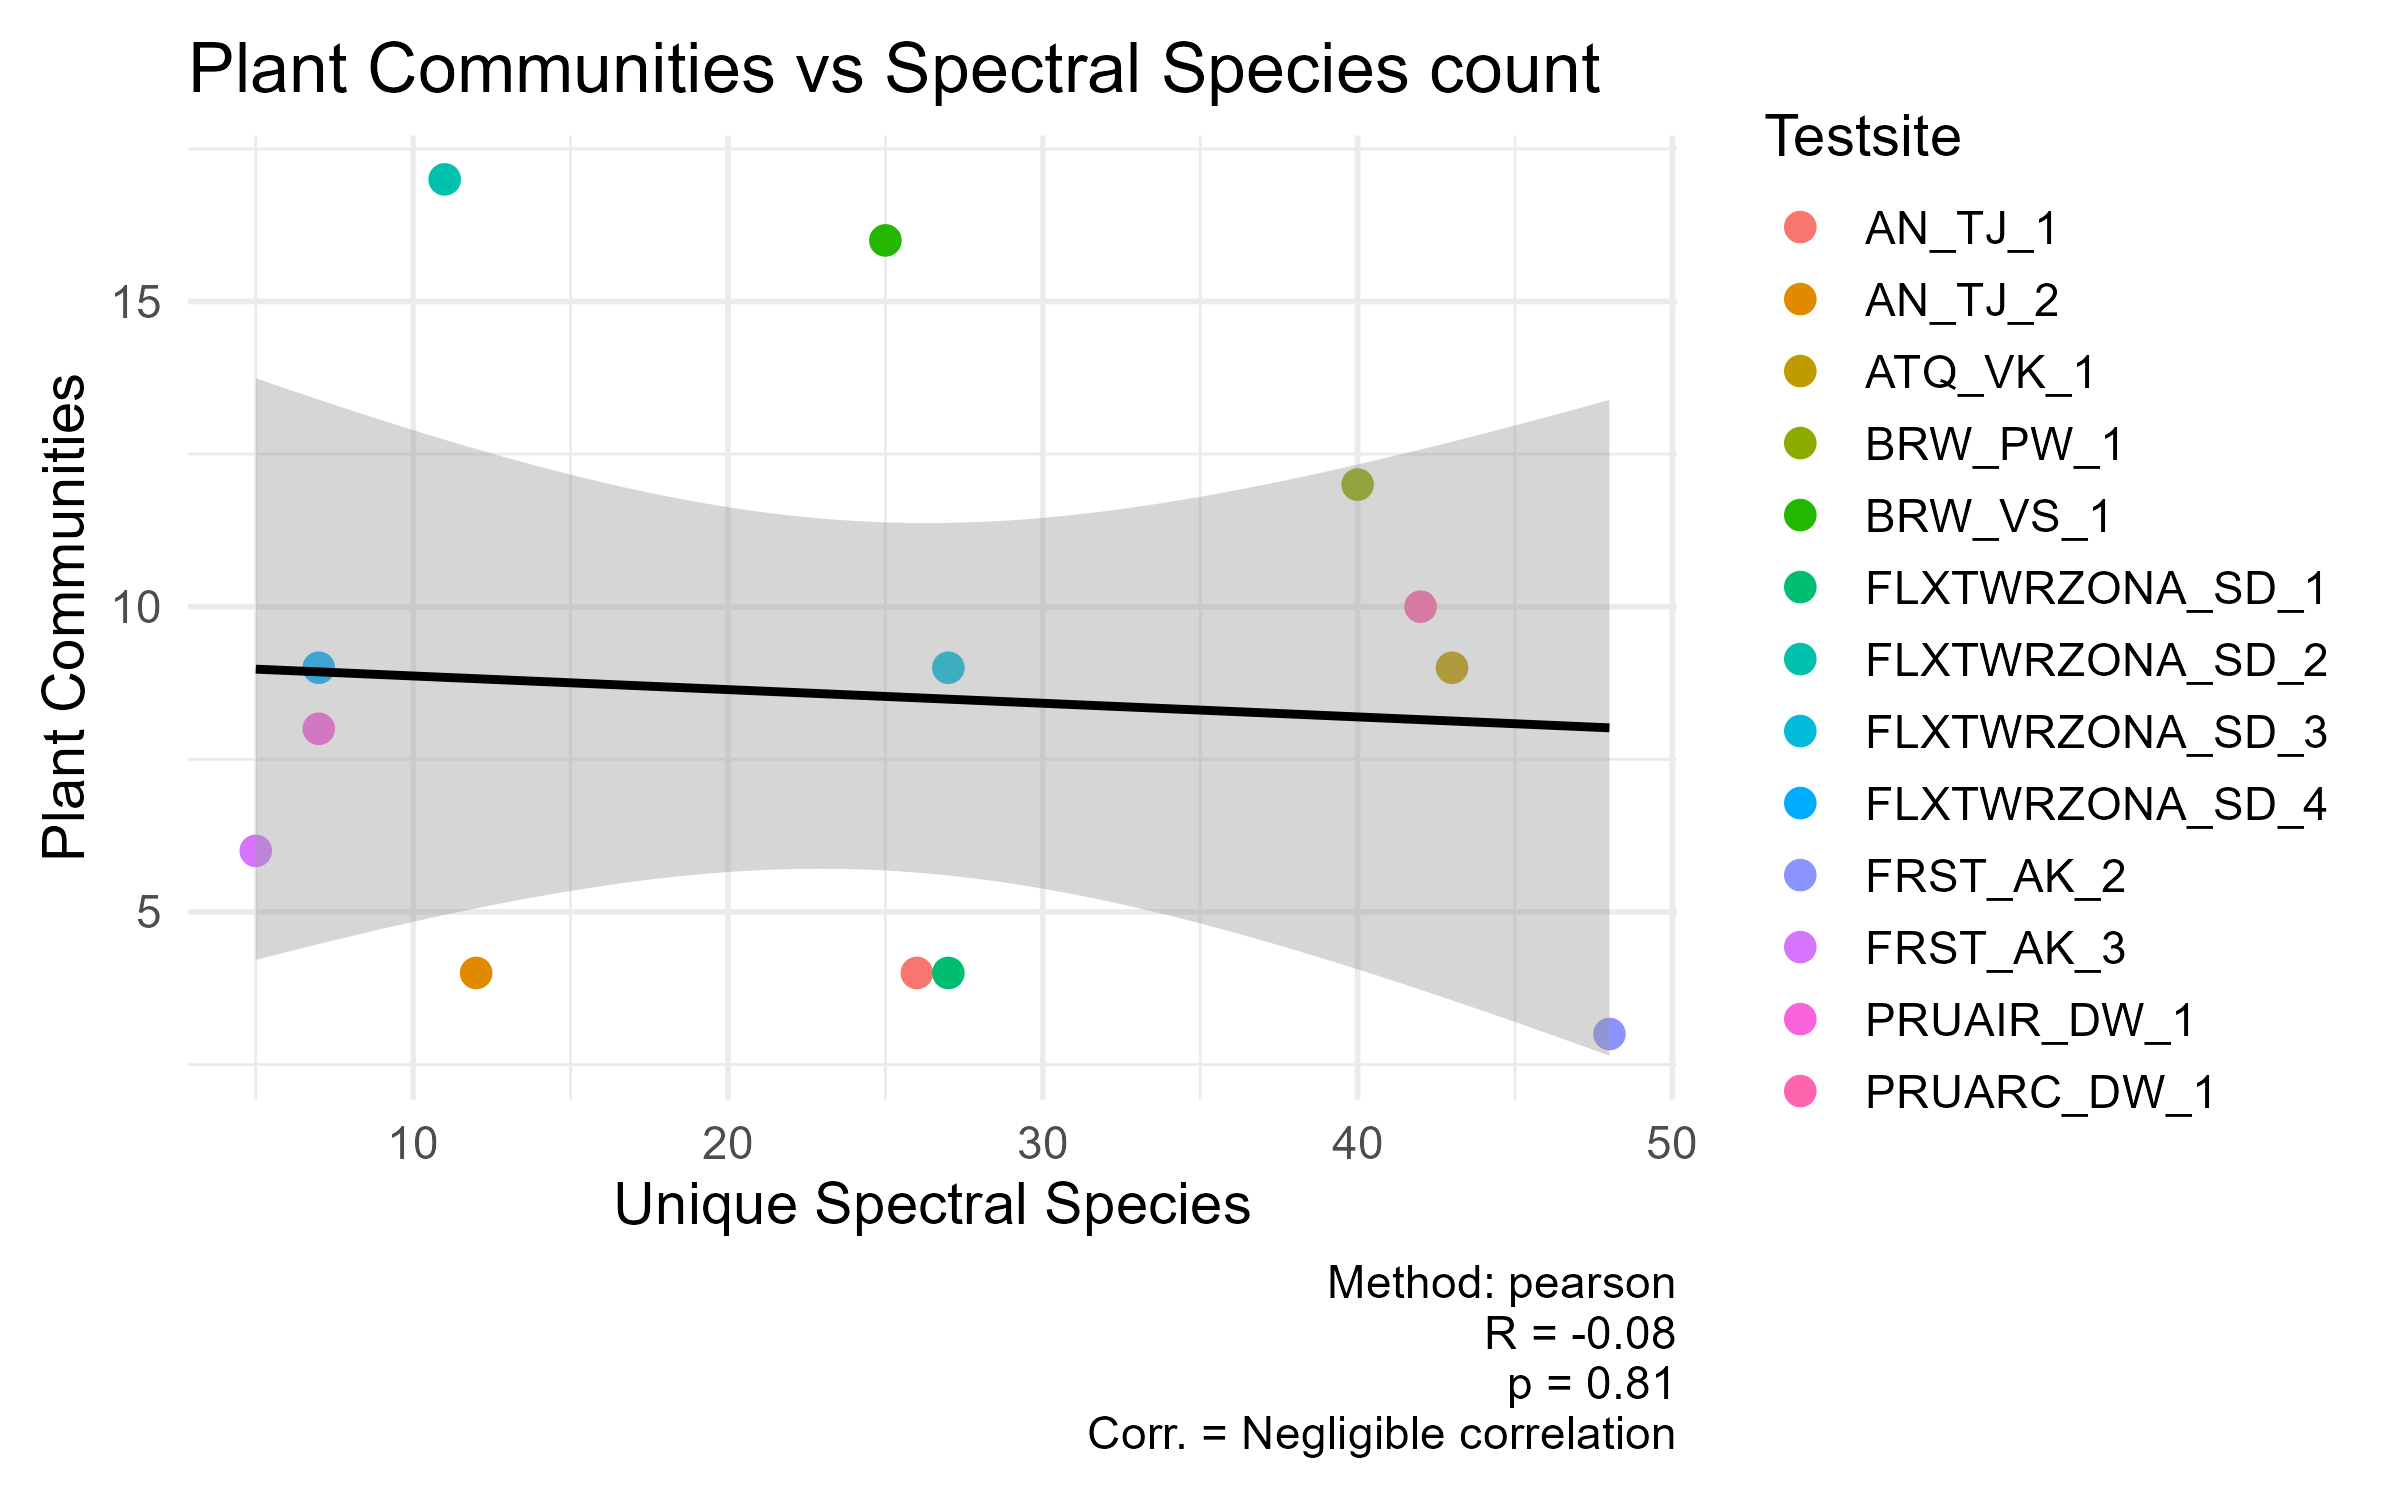
\includegraphics[width=0.9\textwidth]{Figures/WCSS_correlation_plant_communities.png} % Replace with your actual image path
    \caption{The Pearson correlation test over all test sites shows a negligible correlation between spectral species and plant communities with an $R$ value of -0.08 and a $p$-value of 0.81.}
    \label{fig:WCSS_correlation_plant_communities}
\end{figure}

\begin{table}[ht]
\centering
\caption{Summary of linear regression model predicting plant community richness from spectral species richness over all test sites}
\begin{tabular}{lcccc}
\hline
\textbf{Predictor} & \textbf{Estimate} & \textbf{Std. Error} & \textbf{t value} & \textbf{Pr($>$$|$t$|$)} \\
\hline
Intercept & 9.08876 & 2.53324 & 3.588 & \textbf{0.00426**} \\
Unique Spectral Species & -0.02236 & 0.08845 & -0.253 & 0.80512 \\
\hline
\multicolumn{5}{l}{\textit{Residual standard error:} 4.669 on 11 degrees of freedom} \\
\multicolumn{5}{l}{\textit{Multiple R-squared:} 0.005774 \quad \textit{Adjusted R-squared:} -0.08461} \\
\multicolumn{5}{l}{\textit{F-statistic:} 0.06389 on 1 and 11 DF, \quad \textit{p-value:} 0.8051} \\
\hline
\end{tabular}
\label{tab:lm_plant_community_spectral}
\end{table}

\subsection{Results for Group C/D}
The Pearson correlation analysis for Group C/D indicated a weak negative correlation between spectral species richness and plant community richness, with a correlation coefficient of $R$ = -0.2 (Fig. \ref{fig:WCSS_correlation_plant_communities_part_c_d}).
\begin{figure}[H]
    \centering
    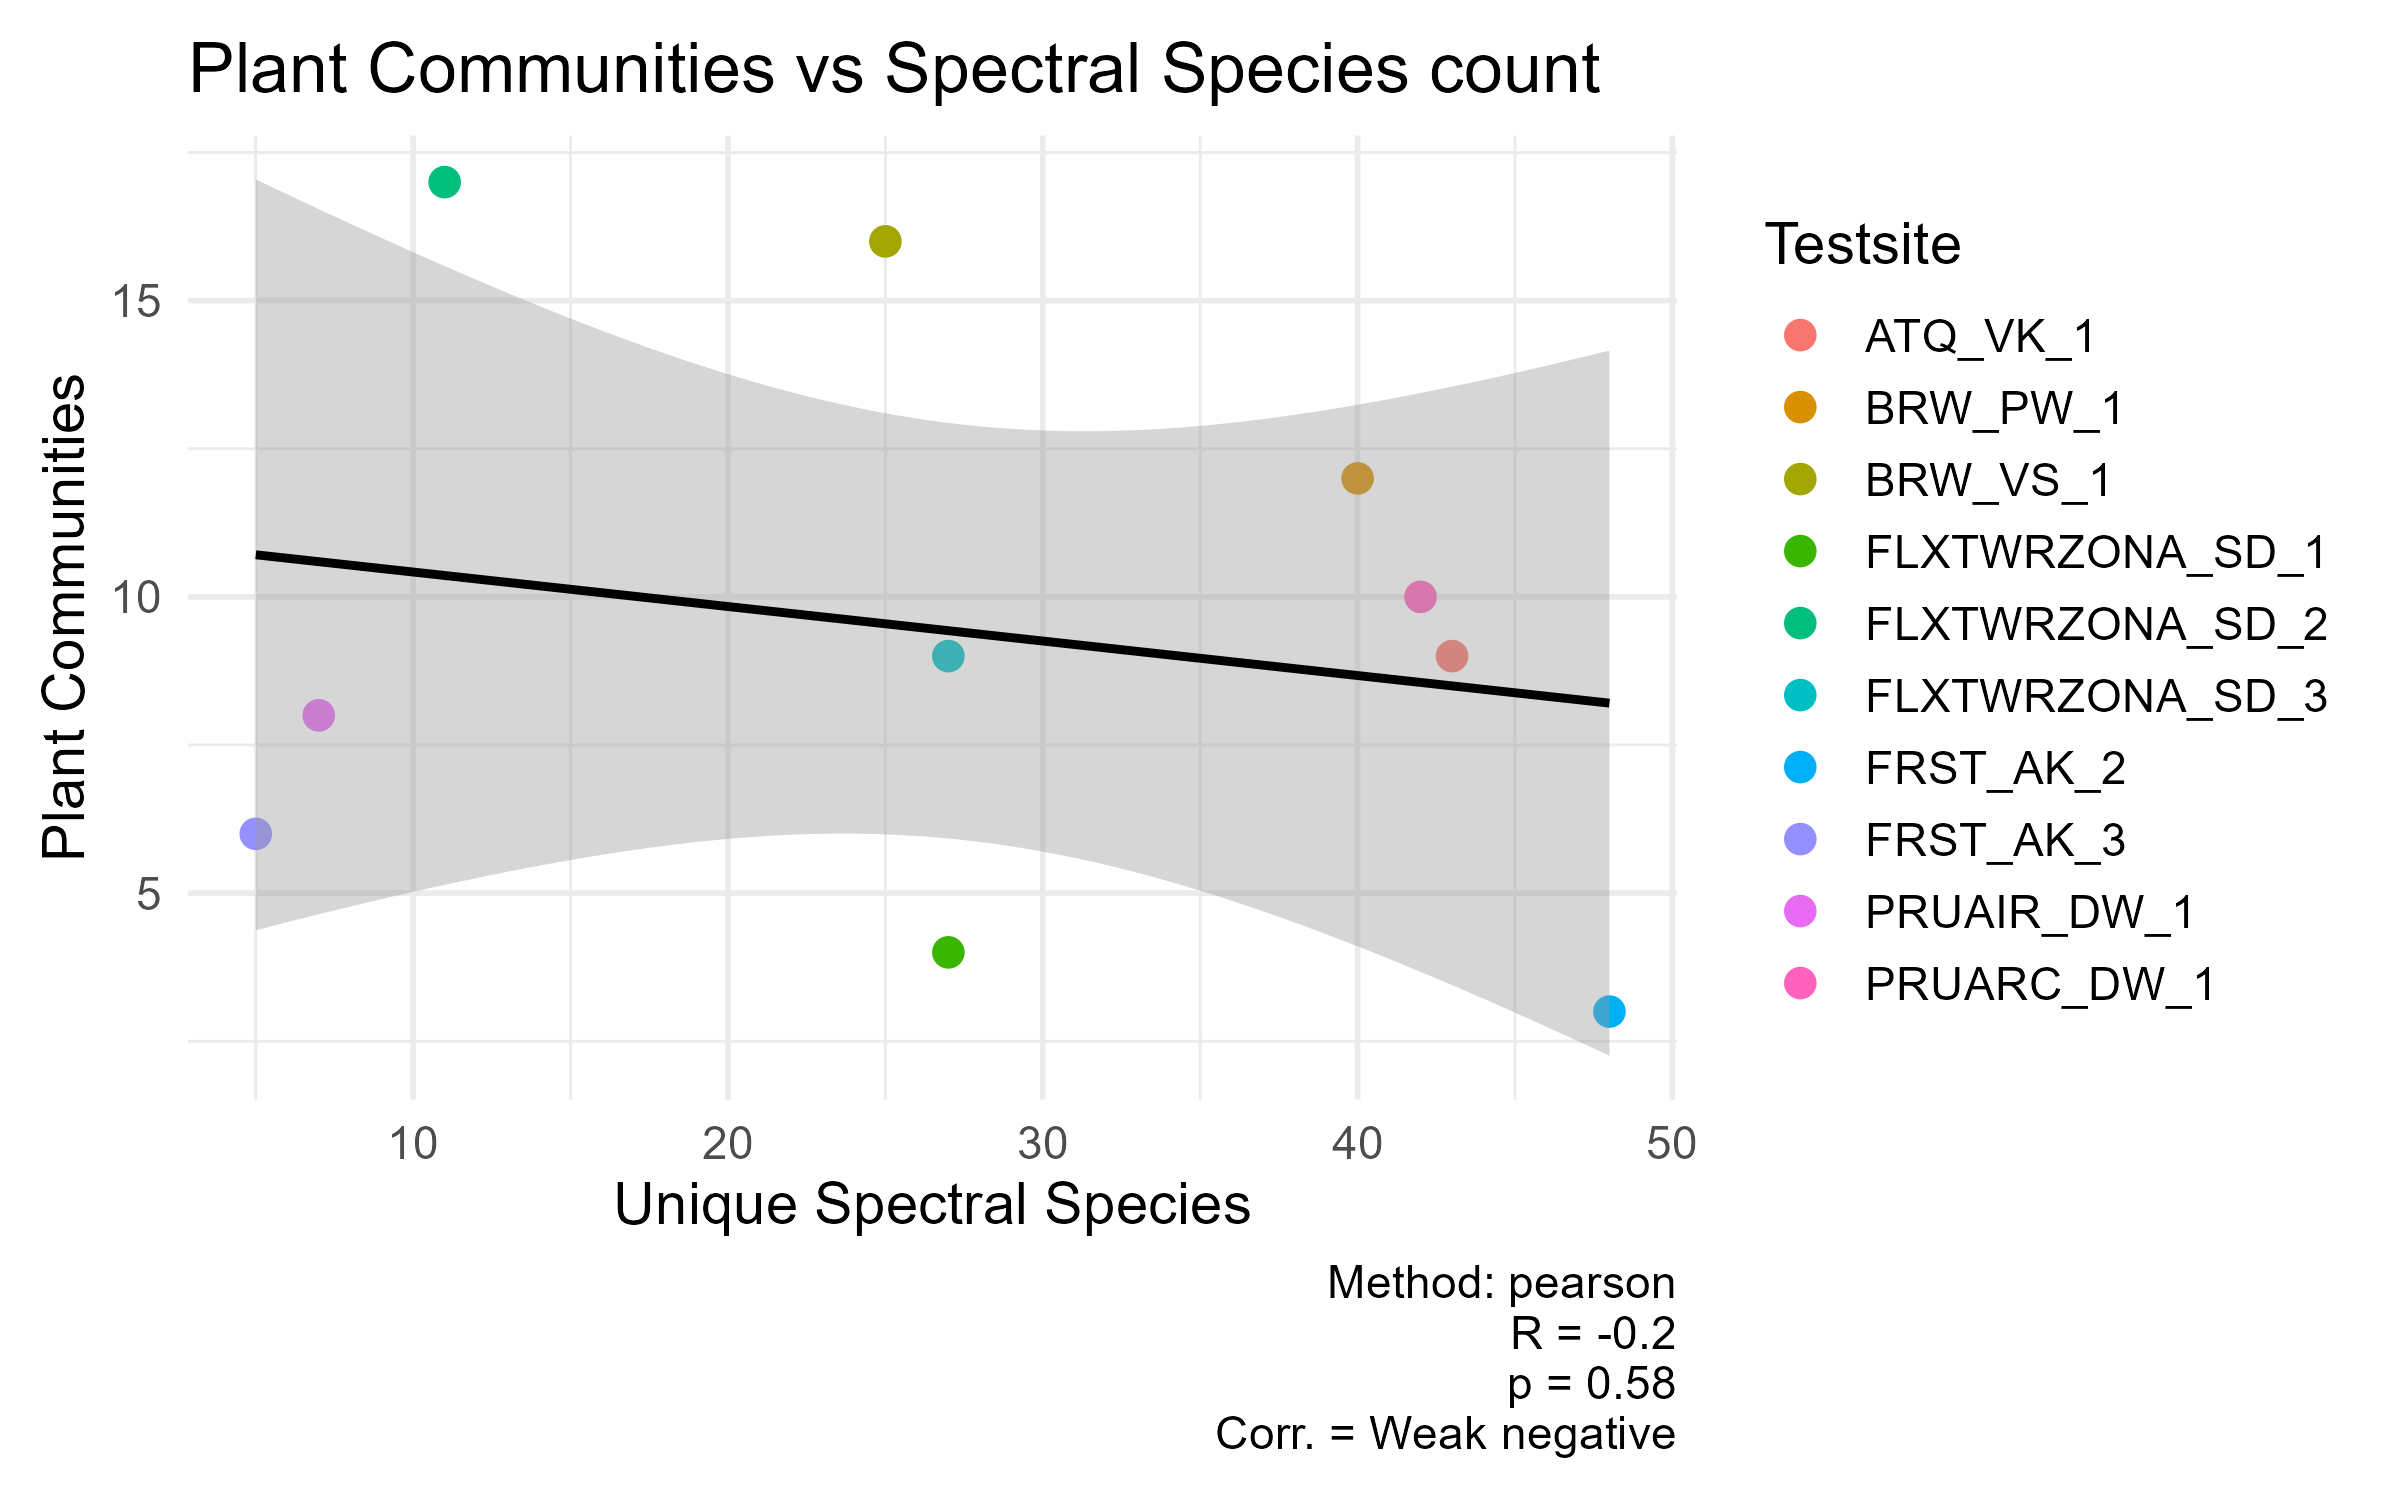
\includegraphics[width=0.9\textwidth]{Figures/WCSS_correlation_plant_communities_part_c_d.png} % Replace with your actual image path
    \caption{The Pearson correlation test within Group C/D shows a weak negative correlation between spectral species and plant communities with an $R$ value of -0.2 and a $p$-value of 0.58.}
    \label{fig:WCSS_correlation_plant_communities_part_c_d}
\end{figure}

\begin{table}[ht]
\centering
\caption{Summary of linear regression model predicting plant community richness from spectral species richness for Group C/D}
\begin{tabular}{lcccc}
\hline
\textbf{Predictor} & \textbf{Estimate} & \textbf{Std. Error} & \textbf{t value} & \textbf{Pr($>$$|$t$|$)} \\
\hline
Intercept & 11.00134 & 3.18381 & 3.455 & \textbf{0.00863**} \\
Unique Spectral Species & -0.05823 & 0.10173 & -0.572 & 0.58277 \\
\hline
\multicolumn{5}{l}{\textit{Residual standard error:} 4.807 on 8 degrees of freedom} \\
\multicolumn{5}{l}{\textit{Multiple R-squared:} 0.03935 \quad \textit{Adjusted R-squared:} -0.08074} \\
\multicolumn{5}{l}{\textit{F-statistic:} 0.3277 on 1 and 8 DF, \quad \textit{p-value:} 0.5828} \\
\hline
\end{tabular}
\label{tab:lm_plantspecies_spectral}
\end{table}


\subsection{Results for Group E}
The Pearson correlation analysis for Group E indicated a strong negative correlation between spectral species richness and plant community richness, with a correlation coefficient of $R$ = -0.82 (Fig. \ref{fig:WCSS_correlation_plant_communities_part_e}).
\begin{figure}[H]
    \centering
    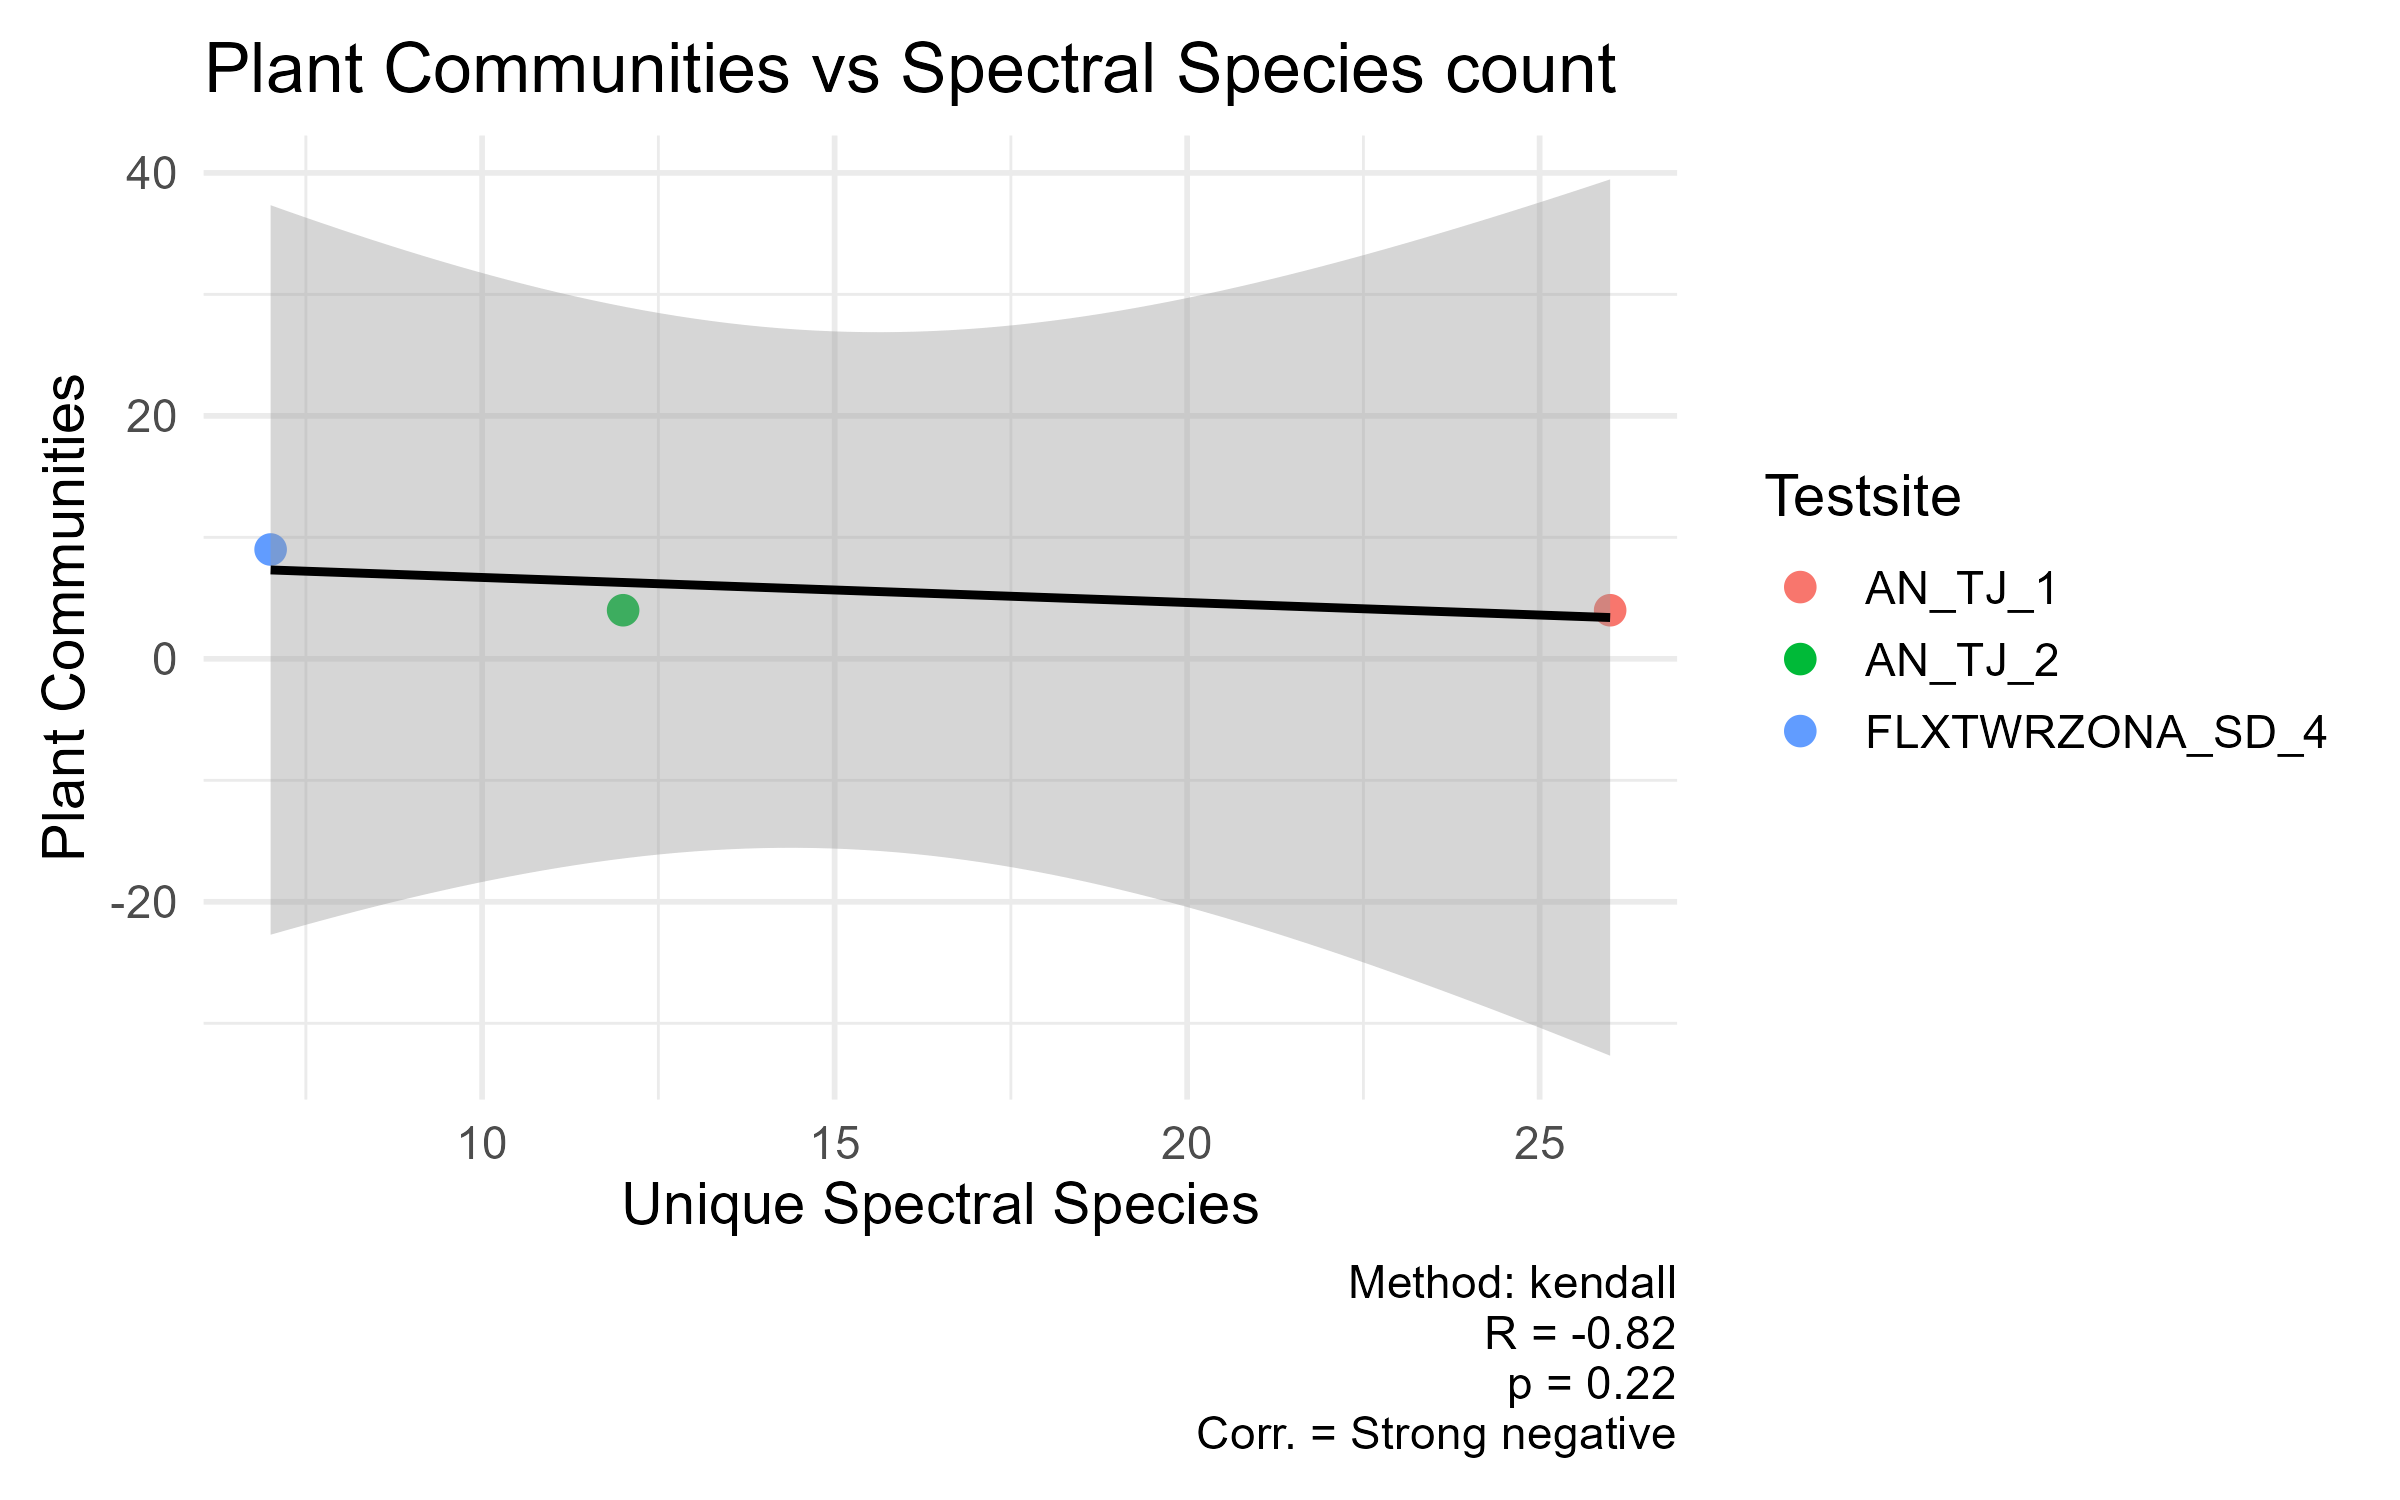
\includegraphics[width=0.9\textwidth]{Figures/WCSS_correlation_plant_communities_part_e.png} % Replace with your actual image path
    \caption{The Kendall's tau correlation test within Group E shows a strong negative correlation between spectral species and plant communities with an $R$ value of -0.82 and a $p$-value of 0.22.}
    \label{fig:WCSS_correlation_plant_communities_part_e}
\end{figure}

\begin{table}[ht]
\centering
\caption{Summary of linear regression model predicting plant community richness from spectral species richness for Group E}
\begin{tabular}{lcccc}
\hline
\textbf{Predictor} & \textbf{Estimate} & \textbf{Std. Error} & \textbf{t value} & \textbf{Pr($>$$|$t$|$)} \\
\hline
Intercept & 8.7595 & 3.5456 & 2.471 & 0.245 \\
Unique Spectral Species & -0.2062 & 0.2083 & -0.990 & 0.503 \\
\hline
\multicolumn{5}{l}{\textit{Residual standard error:} 2.902 on 1 degrees of freedom} \\
\multicolumn{5}{l}{\textit{Multiple R-squared:} 0.4948 \quad \textit{Adjusted R-squared:} -0.01031} \\
\multicolumn{5}{l}{\textit{F-statistic:} 0.9796 on 1 and 1 DF, \quad \textit{p-value:} 0.5033} \\
\hline
\end{tabular}
\label{tab:lm_plantspecies_spectral}
\end{table}

\section{Habitat types - spectral species}
\subsection{Results over all test sites}
The Pearson correlation analysis over all test sites indicated a weak positive correlation between spectral species richness and habitat type richness, with a correlation coefficient of $R$ = 0.29 (Fig. \ref{fig:WCSS_correlation_habitat_types}).

\begin{figure}[H]
    \centering
    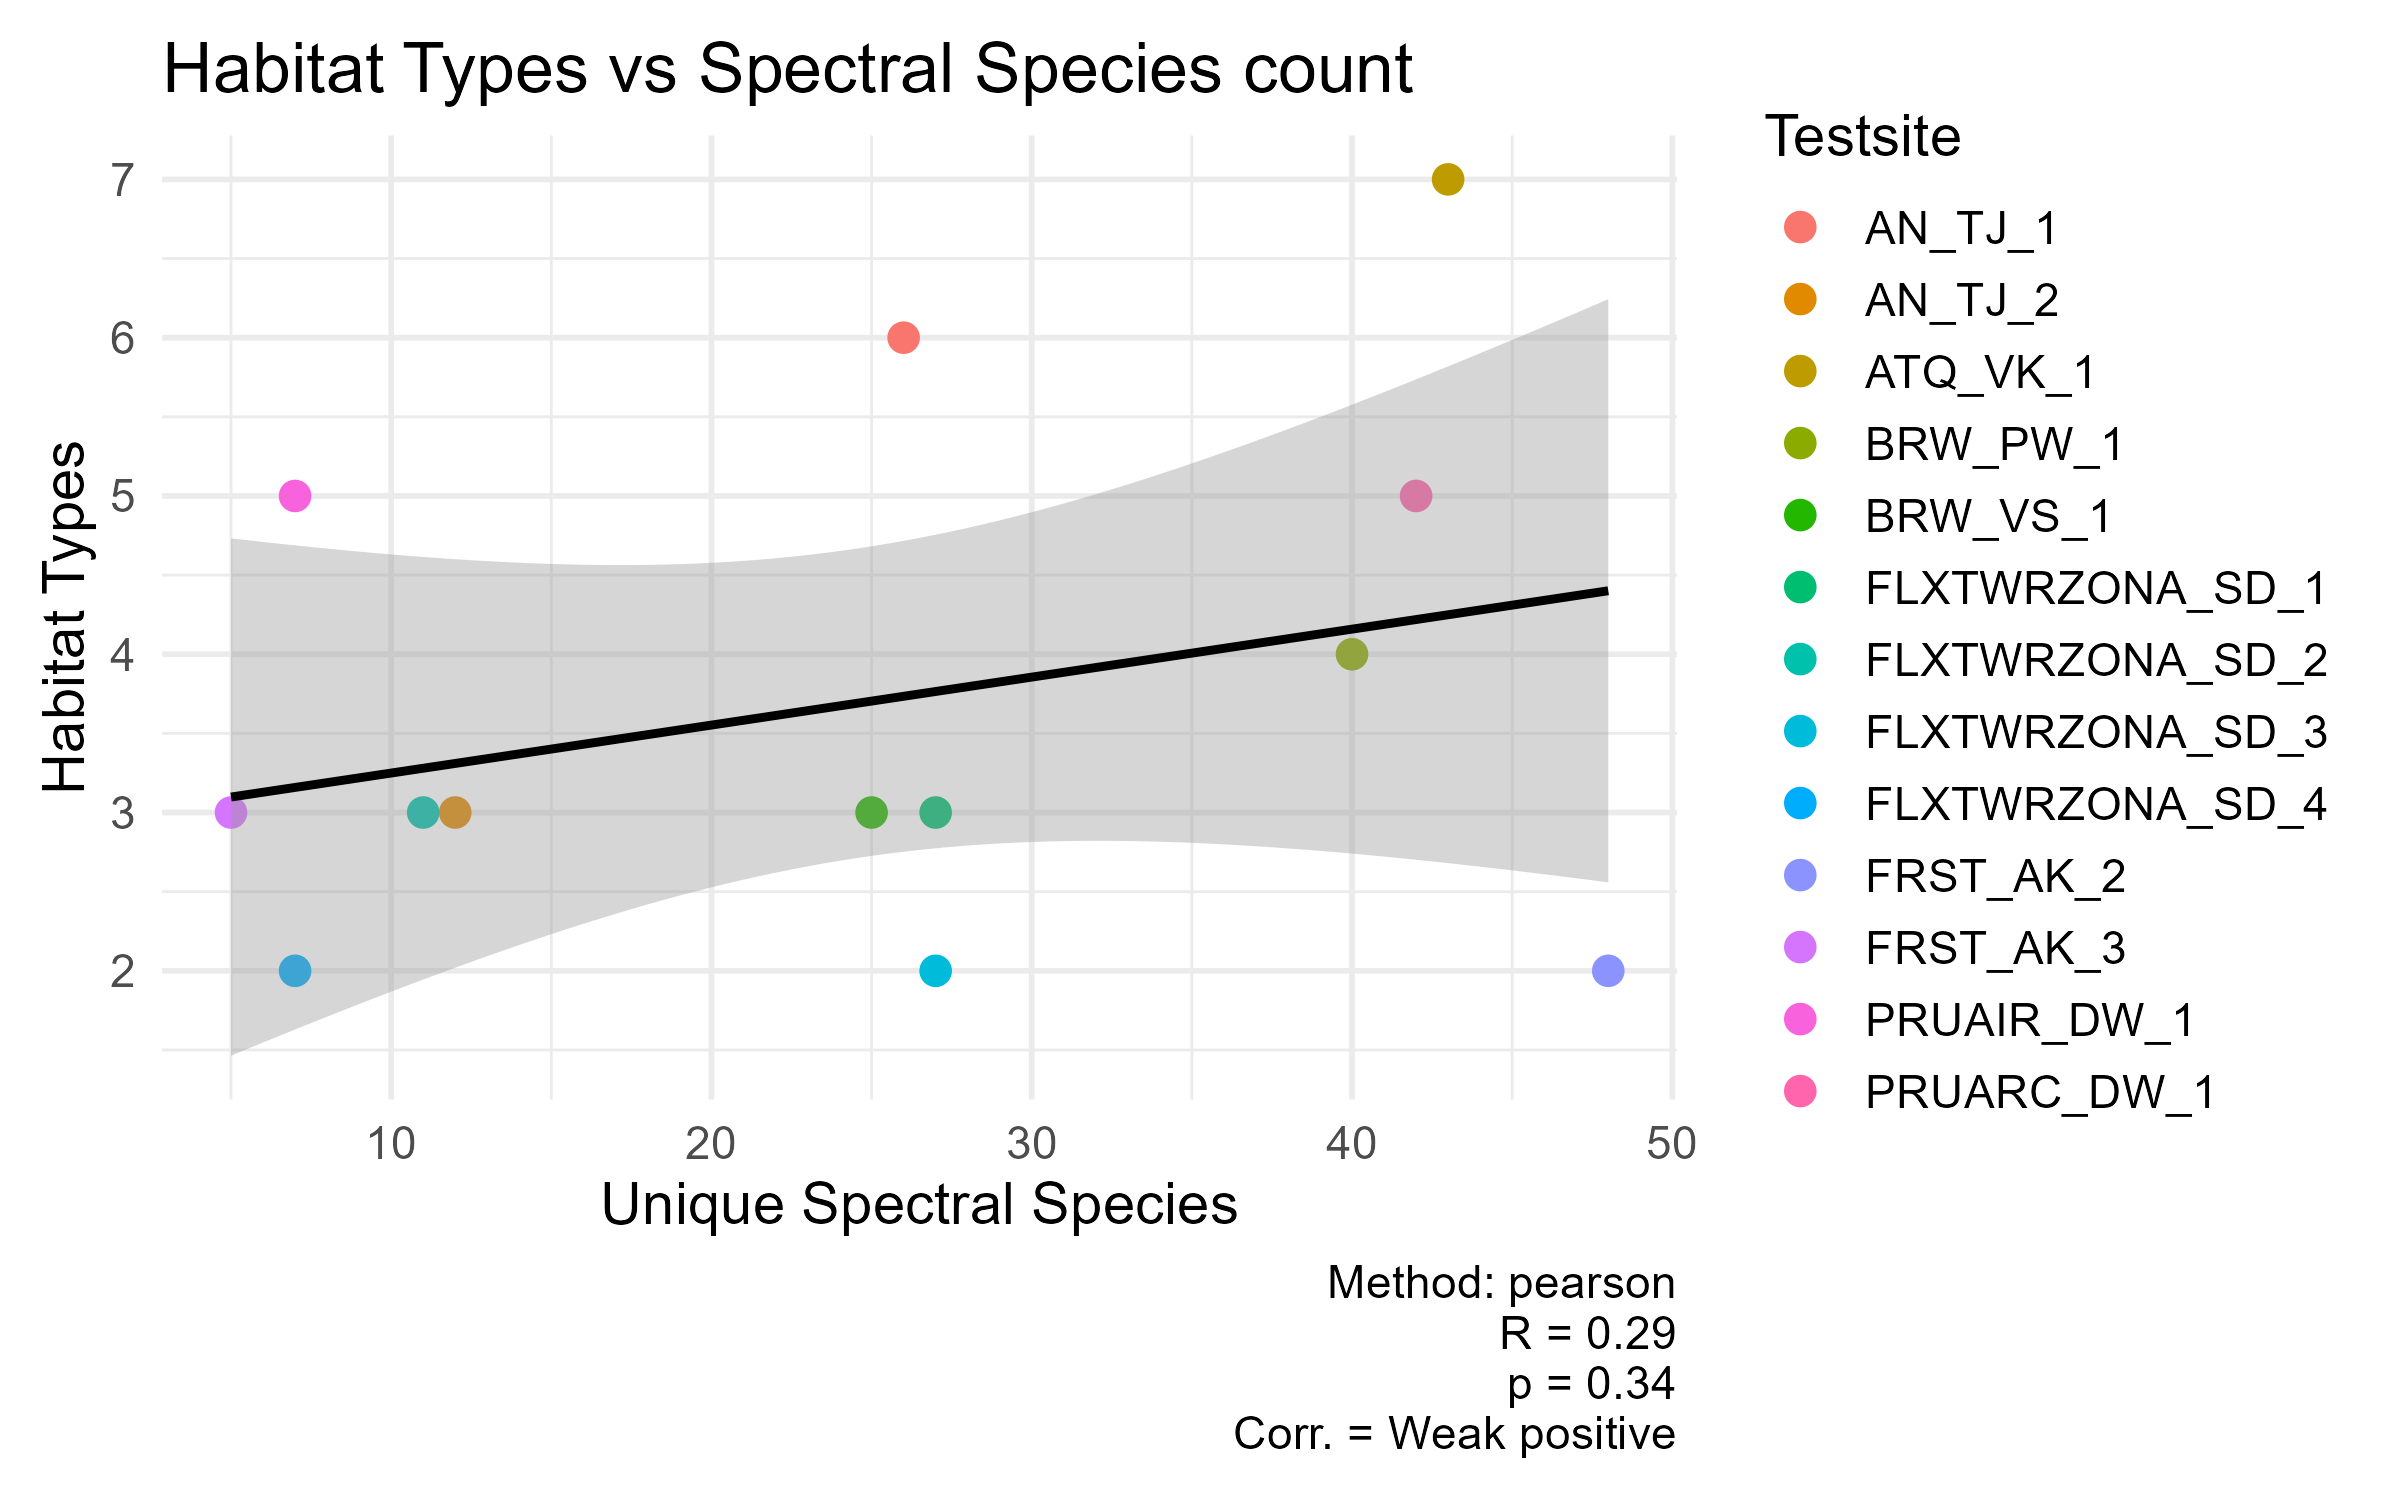
\includegraphics[width=0.9\textwidth]{Figures/WCSS_correlation_habitat_types.png} % Replace with your actual image path
    \caption{The Pearson correlation test over all test sites shows a weak positive correlation between spectral species and habitat type with an $R$ value of 0.29 and a $p$-value of 0.34.}
    \label{fig:WCSS_correlation_habitat_types}
\end{figure}

\begin{table}[ht]
\centering
\caption{Summary of linear regression model predicting habitat type richness from spectral species richness over all test sites}
\begin{tabular}{lcccc}
\hline
\textbf{Predictor} & \textbf{Estimate} & \textbf{Std. Error} & \textbf{t value} & \textbf{Pr($>$$|$t$|$)} \\
\hline
Intercept & 2.94635 & 0.86879 & 3.391 & \textbf{0.00602**} \\
Unique Spectral Species & 0.03030 & 0.03033 & 0.999 & 0.33925 \\
\hline
\multicolumn{5}{l}{\textit{Residual standard error:} 1.601 on 11 degrees of freedom} \\
\multicolumn{5}{l}{\textit{Multiple R-squared:} 0.08319 \quad \textit{Adjusted R-squared:} -0.0001603} \\
\multicolumn{5}{l}{\textit{F-statistic:} 0.9981 on 1 and 11 DF, \quad \textit{p-value:} 0.3392} \\
\hline
\end{tabular}
\label{tab:lm_habitat_type_spectral}
\end{table}

\subsection{Results for Group C/D}
The Pearson correlation analysis for Group C/D indicated a weak positive correlation between spectral species richness and habitat type richness, with a correlation coefficient of $R$ = 0.19 (Fig. \ref{fig:WCSS_correlation_habitat_types_part_c_d}).

\begin{figure}[H]
    \centering
    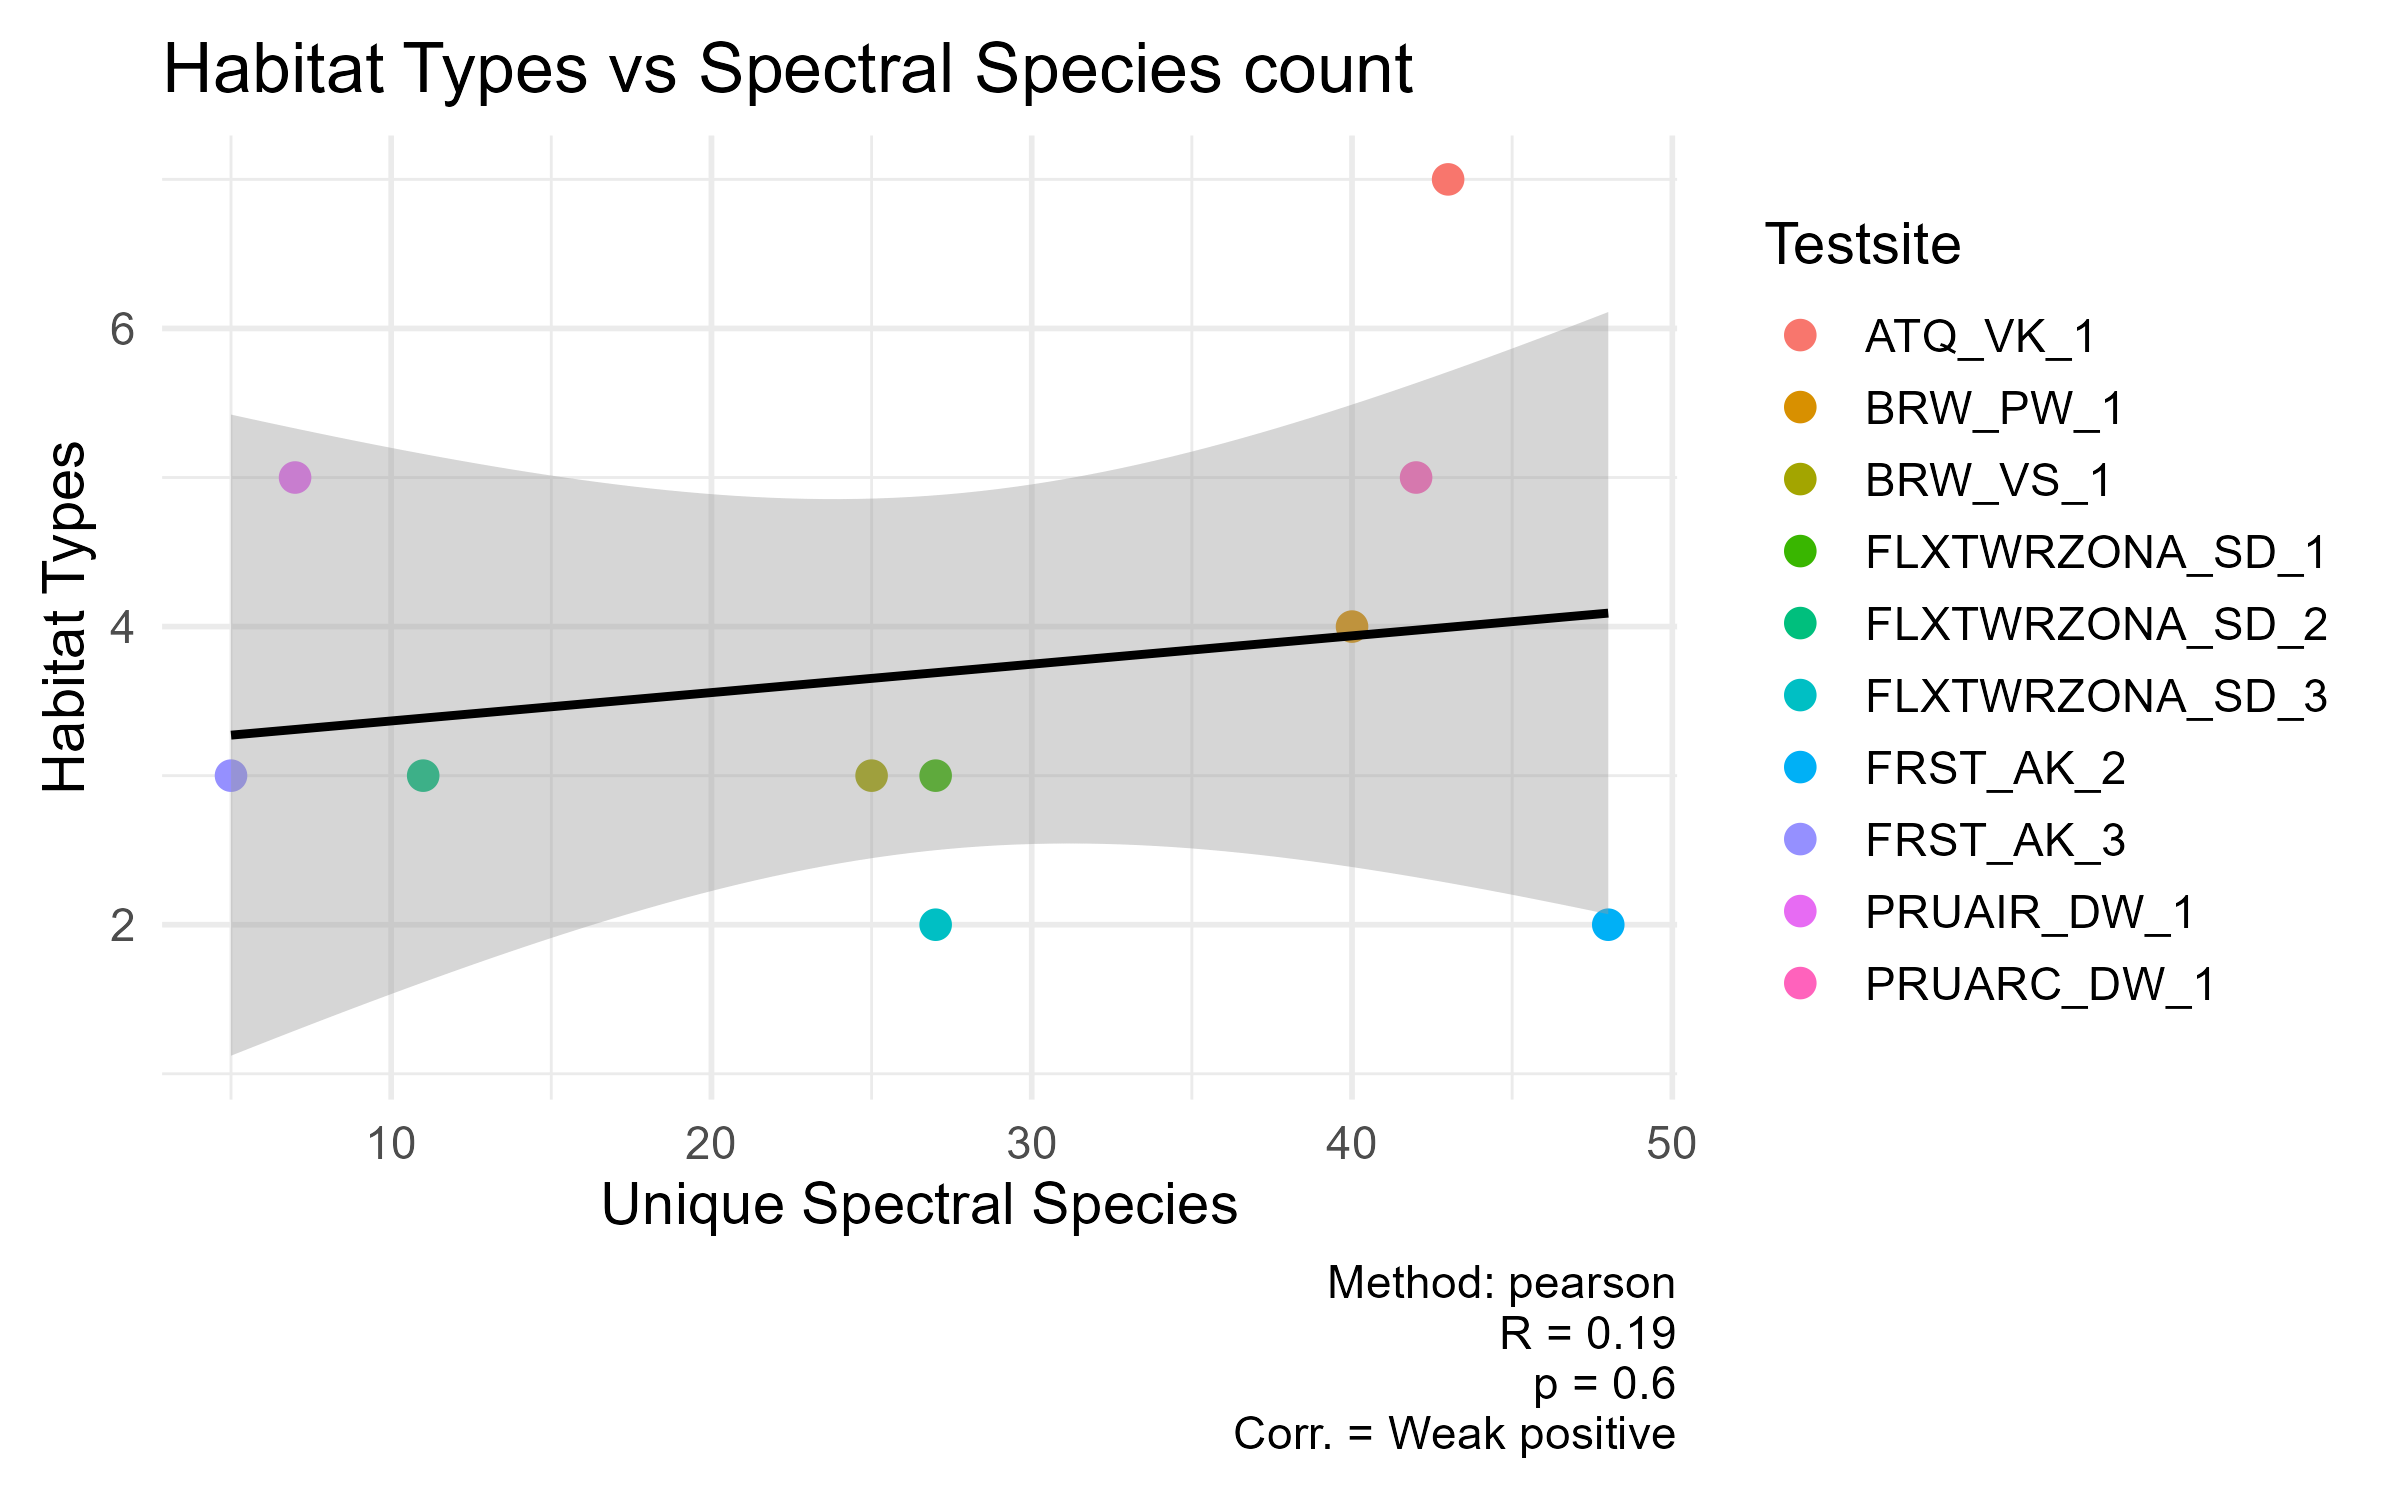
\includegraphics[width=0.9\textwidth]{Figures/WCSS_correlation_habitat_types_part_c_d.png} % Replace with your actual image path
    \caption{The Pearson correlation test within Group C/D shows a weak positive correlation between spectral species and habitat types with an $R$ value of 0.19 and a $p$-value of 0.6.}
    \label{fig:WCSS_correlation_habitat_types_part_c_d}
\end{figure}

\begin{table}[ht]
\centering
\caption{Summary of linear regression model predicting habitat type richness from spectral species richness for Group C/D}
\begin{tabular}{lcccc}
\hline
\textbf{Predictor} & \textbf{Estimate} & \textbf{Std. Error} & \textbf{t value} & \textbf{Pr($>$$|$t$|$)} \\
\hline
Intercept & 3.17648 & 1.08058 & 2.940 & \textbf{0.0187*} \\
Unique Spectral Species & 0.01904 & 0.03453 & 0.551 & 0.5964 \\
\hline
\multicolumn{5}{l}{\textit{Residual standard error:} 1.631 on 8 degrees of freedom} \\
\multicolumn{5}{l}{\textit{Multiple R-squared:} 0.03661 \quad \textit{Adjusted R-squared:} -0.08381} \\
\multicolumn{5}{l}{\textit{F-statistic:} 0.304 on 1 and 8 DF, \quad \textit{p-value:} 0.5964} \\
\hline
\end{tabular}
\label{tab:lm_plantspecies_spectral}
\end{table}


\subsection{Results for Group E}
The Pearson correlation analysis for Group E indicated a very strong positive correlation between spectral species richness and habitat type richness, with a correlation coefficient of $R$ = 1 (Fig. \ref{fig:WCSS_correlation_habitat_types_part_e}).
\begin{figure}[H]
    \centering
    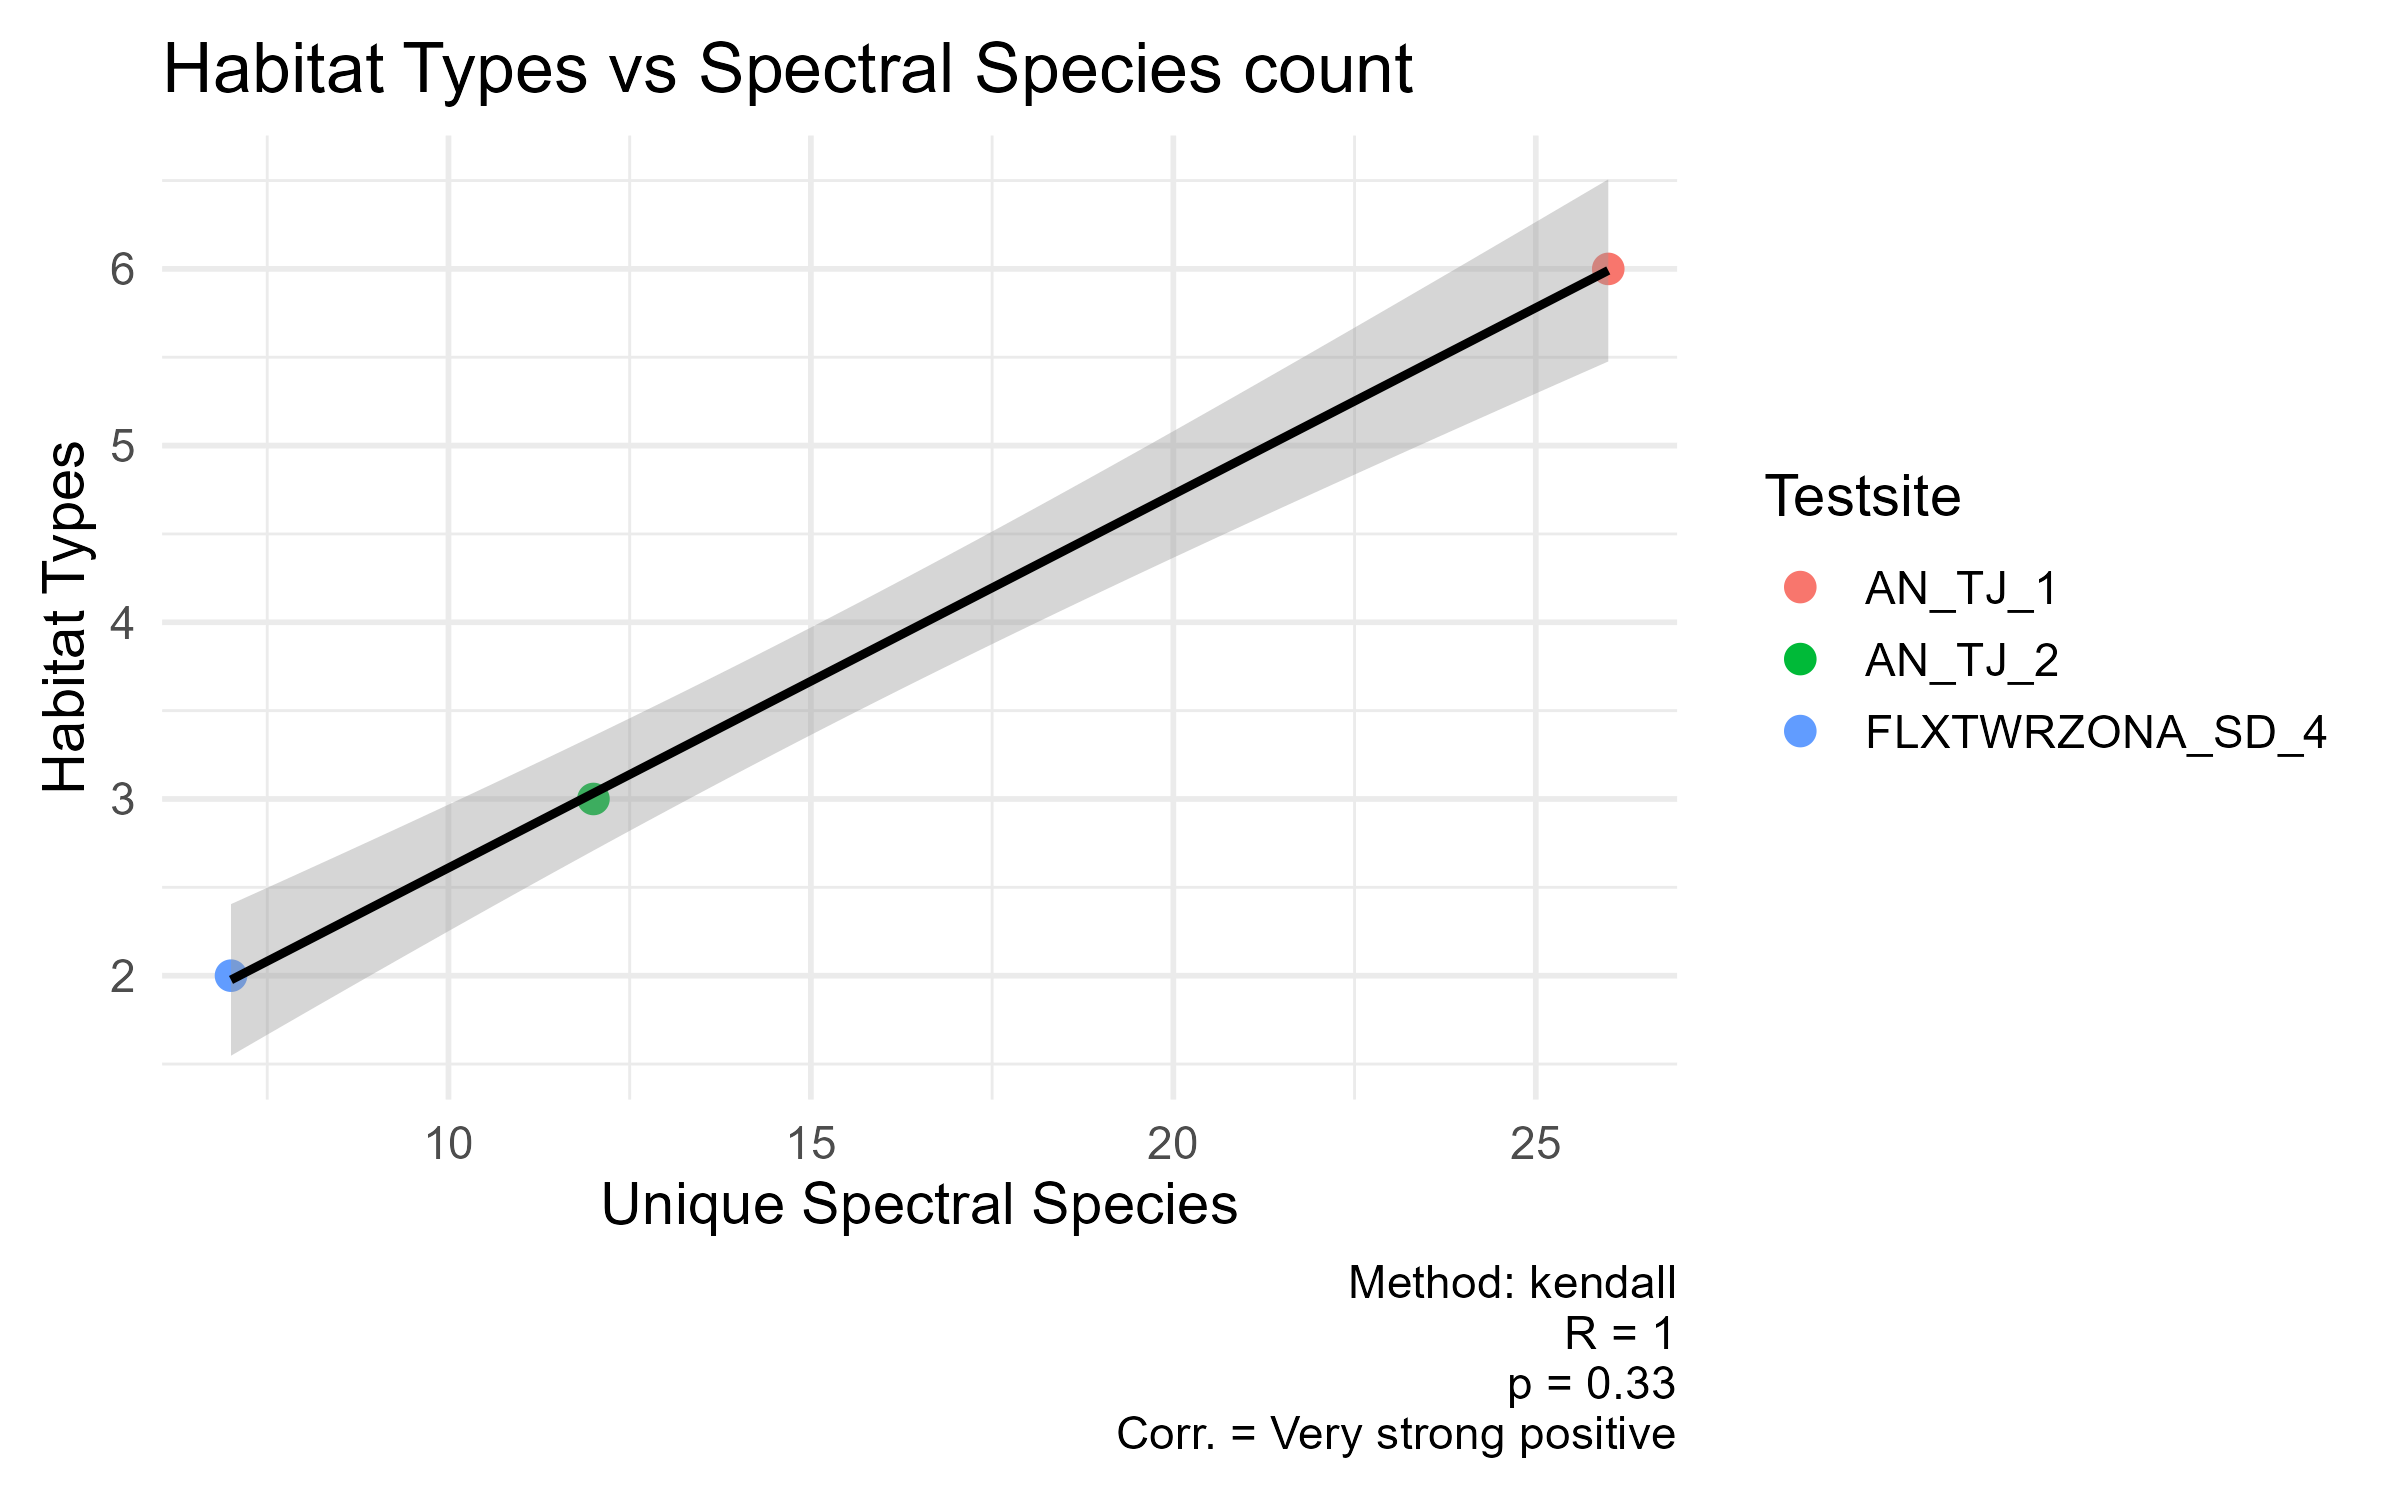
\includegraphics[width=0.9\textwidth]{Figures/WCSS_correlation_habitat_types_part_e.png} % Replace with your actual image path
    \caption{The Kendall's tau correlation test within Group E shows a very strong positive correlation between spectral species and habitat types with an $R$ value of 1 and a $p$-value of 0.33.}
    \label{fig:WCSS_correlation_habitat_types_part_e}
\end{figure}

\begin{table}[ht]
\centering
\caption{Summary of linear regression model predicting habitat type richness from spectral species richness for Group E}
\begin{tabular}{lcccc}
\hline
\textbf{Predictor} & \textbf{Estimate} & \textbf{Std. Error} & \textbf{t value} & \textbf{Pr($>$$|$t$|$)} \\
\hline
Intercept & 0.496564 & 0.050651 & 9.804 & 0.06471 \\
Unique Spectral Species & 0.211340 & 0.002976 & 71.014 & \textbf{0.00896**} \\
\hline
\multicolumn{5}{l}{\textit{Residual standard error:} 0.04145 on 1 degrees of freedom} \\
\multicolumn{5}{l}{\textit{Multiple R-squared:} 0.9998 \quad \textit{Adjusted R-squared:} 0.9996} \\
\multicolumn{5}{l}{\textit{F-statistic:} 5043 on 1 and 1 DF, \quad \textit{p-value:} 0.008964} \\
\hline
\end{tabular}
\label{tab:lm_plantspecies_spectral}
\end{table}

\section{Plot location spectral curves}
--> maybe all the plots belong into the appendix and only the result of the regression analysis is needed here?

\subsection{AN\_TJ\_1}

\begin{figure}[H]
  \centering

  \begin{subfigure}[b]{0.49\textwidth}
    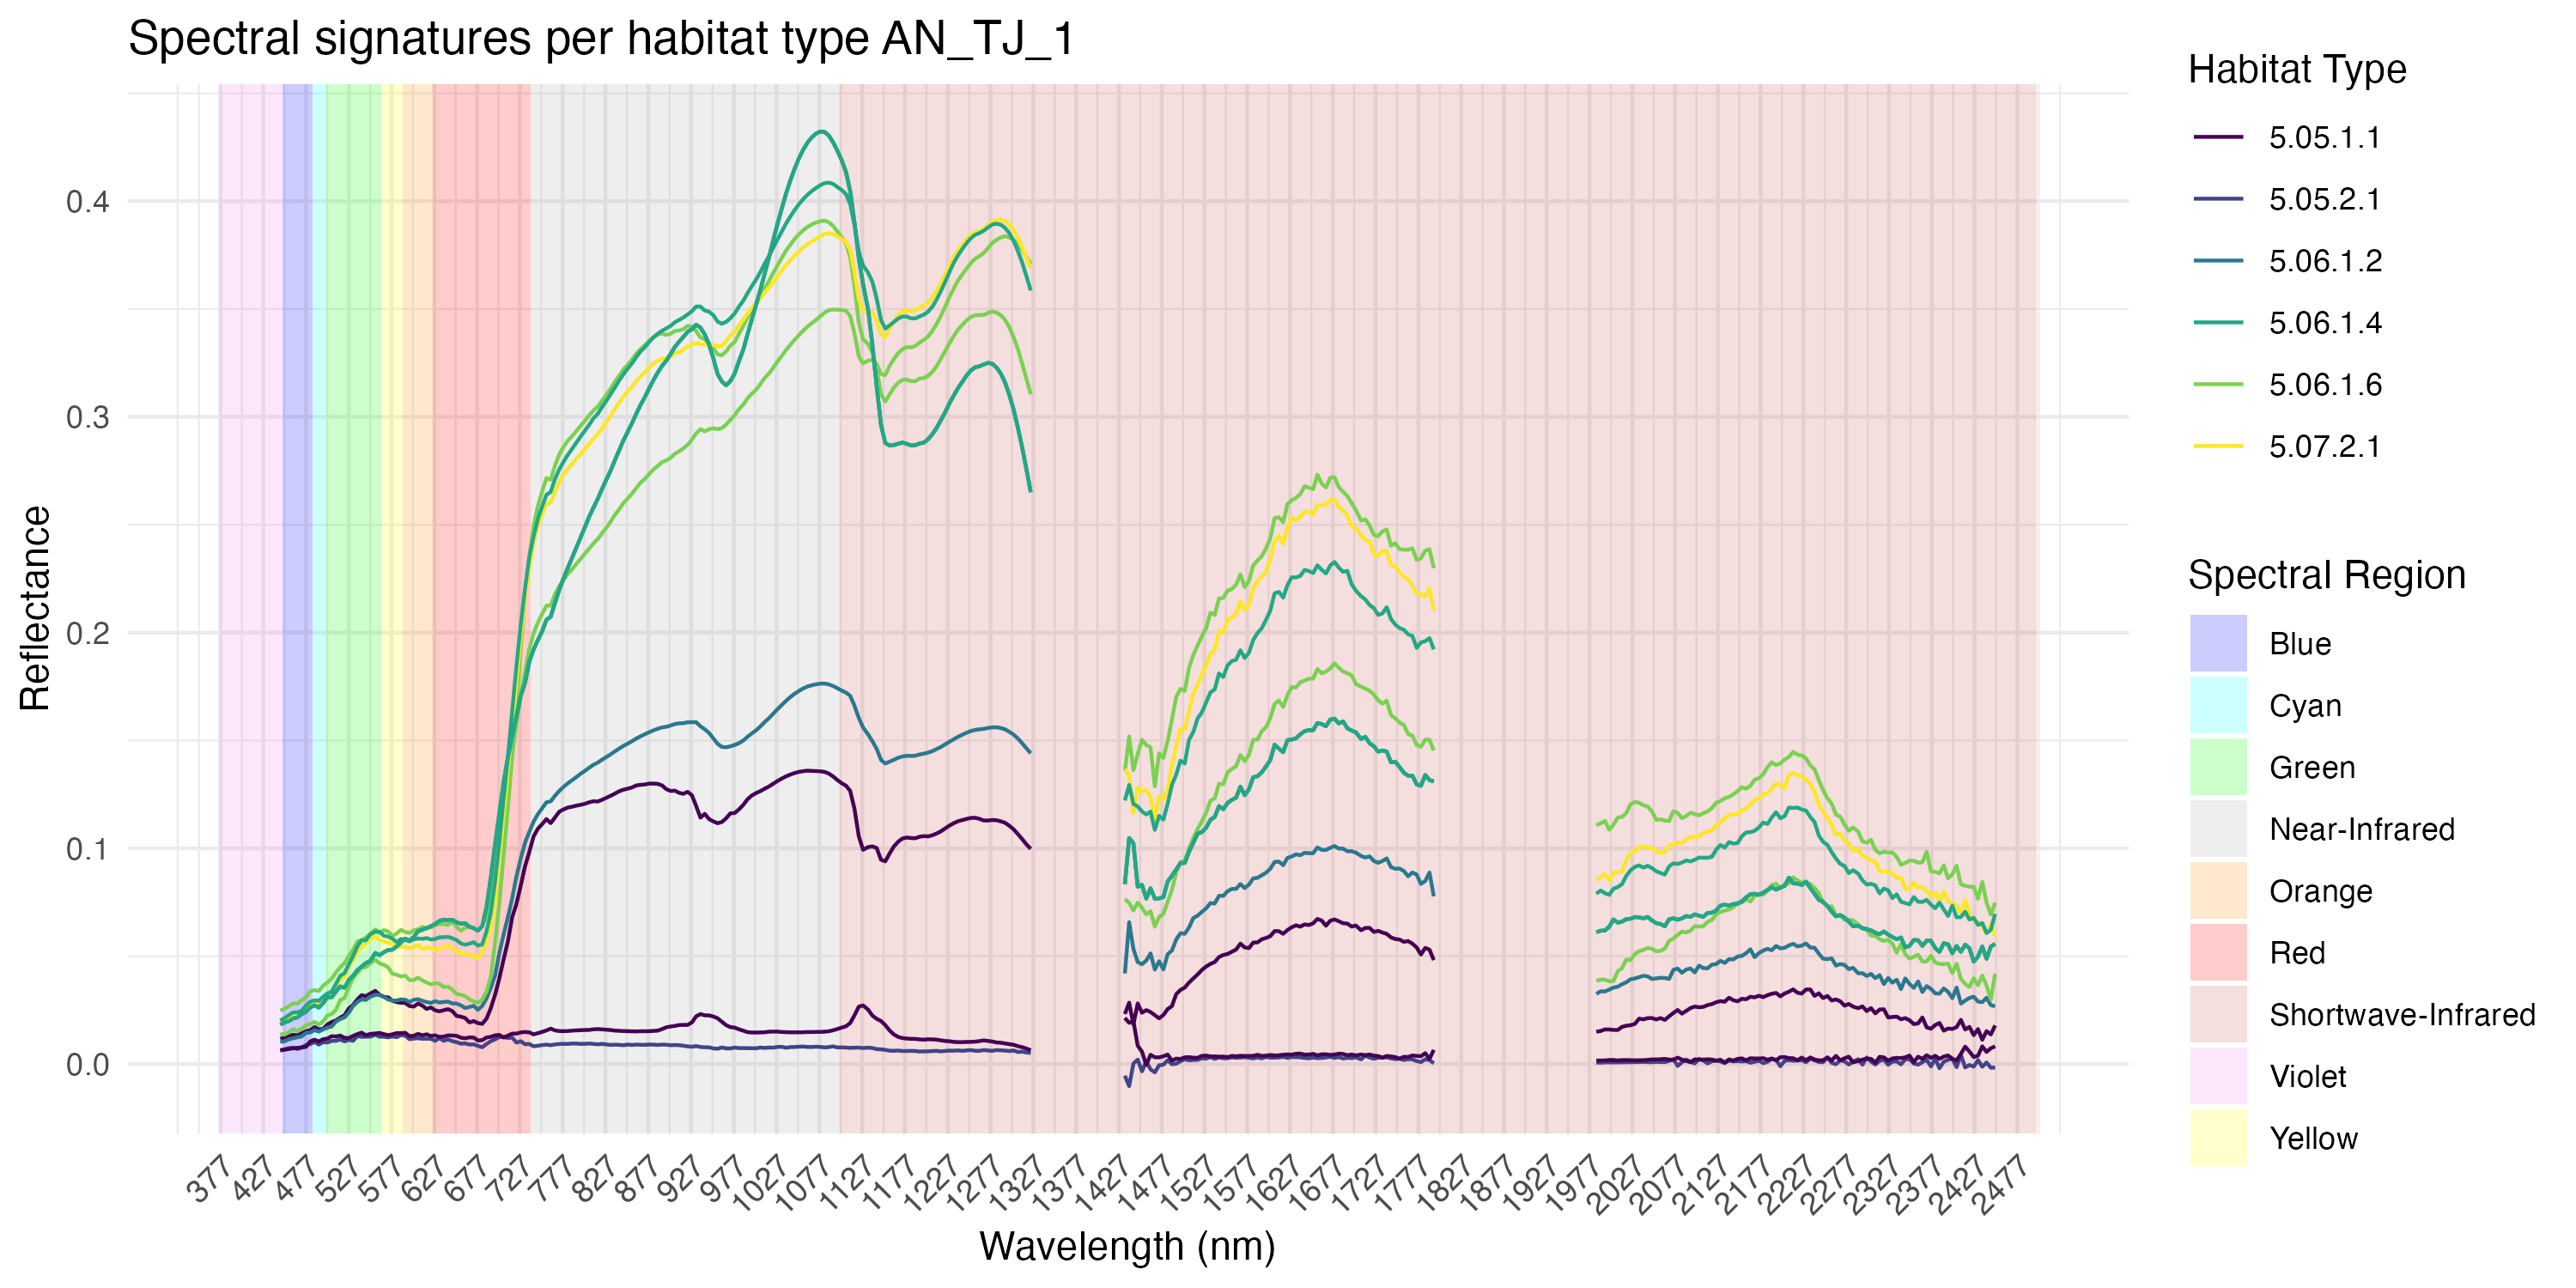
\includegraphics[width=\textwidth]{Figures/spectral_signatures/AN_TJ_1_signature_plot_habitat.png}
    \caption{}
    \label{fig:ss_ht_antj1}
  \end{subfigure}
  \hfill
  \begin{subfigure}[b]{0.49\textwidth}
    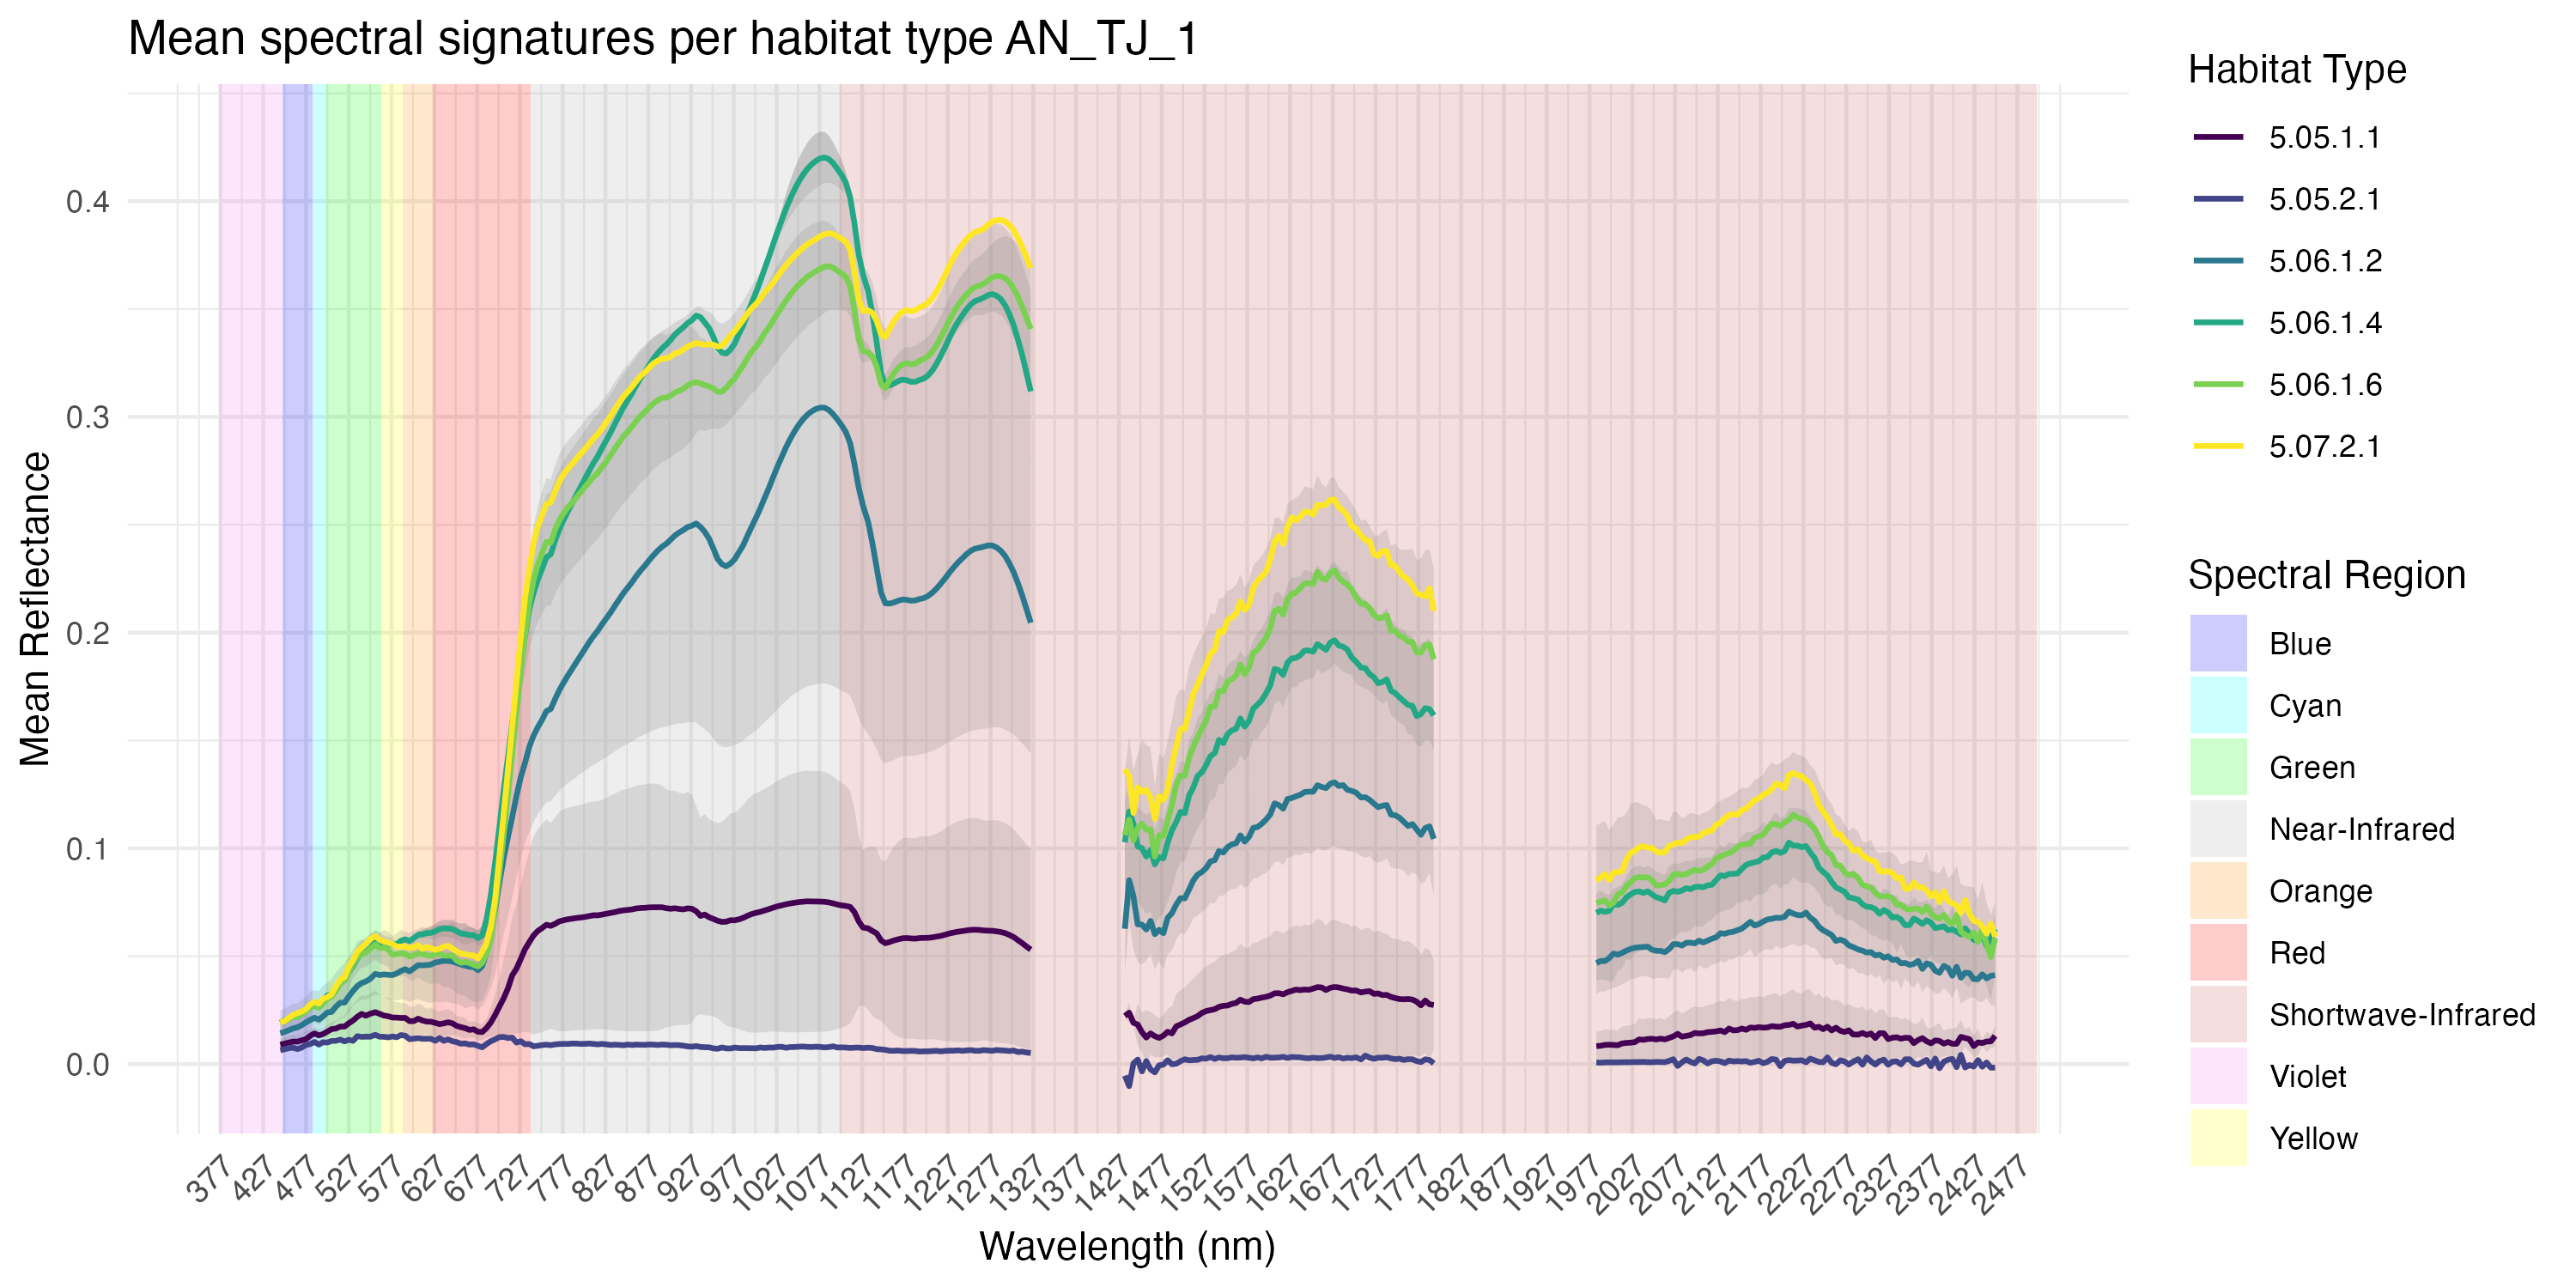
\includegraphics[width=\textwidth]{Figures/spectral_signatures/AN_TJ_1_mean_signature_plot_habitat.png}
    \caption{}
    \label{fig:mss_ht_antj1}
  \end{subfigure}

  \caption{Spectral signature plot \ref{fig:ss_ht_antj1} and mean spectral signature plot \ref{fig:mss_ht_antj1} grouped by habitat type for test site AN\_TJ\_1}
  \label{fig:group_ss_ht_antj1}
\end{figure}

\begin{figure}[H]
  \centering

  \begin{subfigure}[b]{0.49\textwidth}
    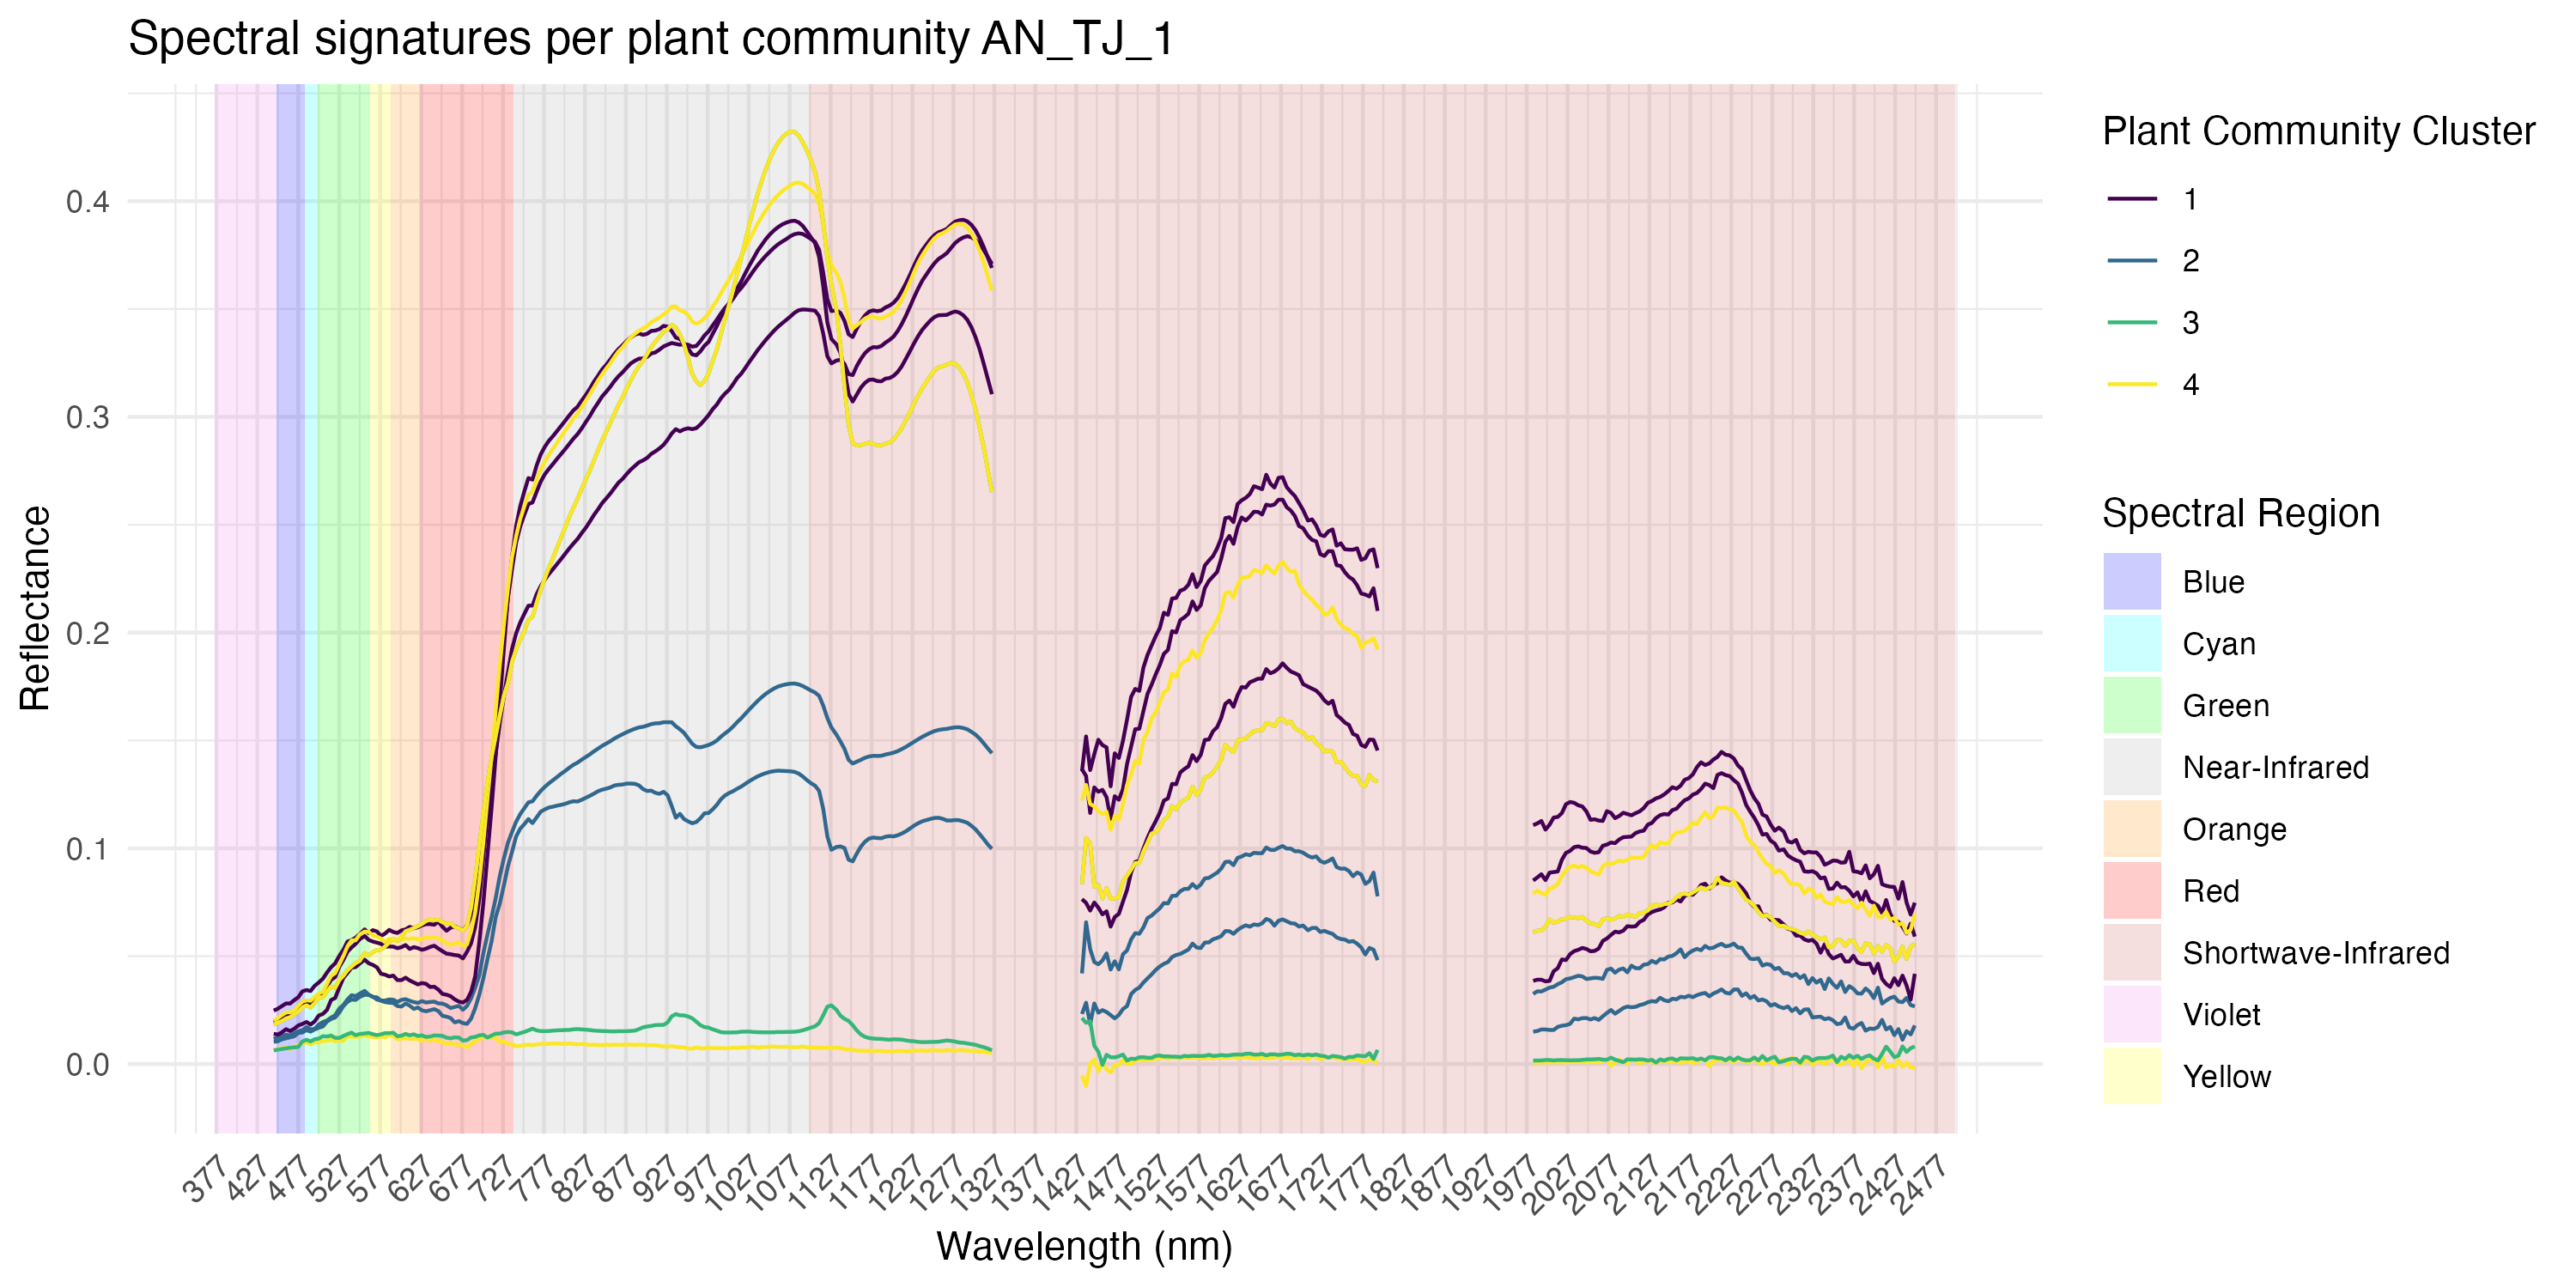
\includegraphics[width=\textwidth]{Figures/spectral_signatures/AN_TJ_1_signature_plot_plant_community.png}
    \caption{}
    \label{fig:ss_pc_antj1}
  \end{subfigure}
  \hfill
  \begin{subfigure}[b]{0.49\textwidth}
    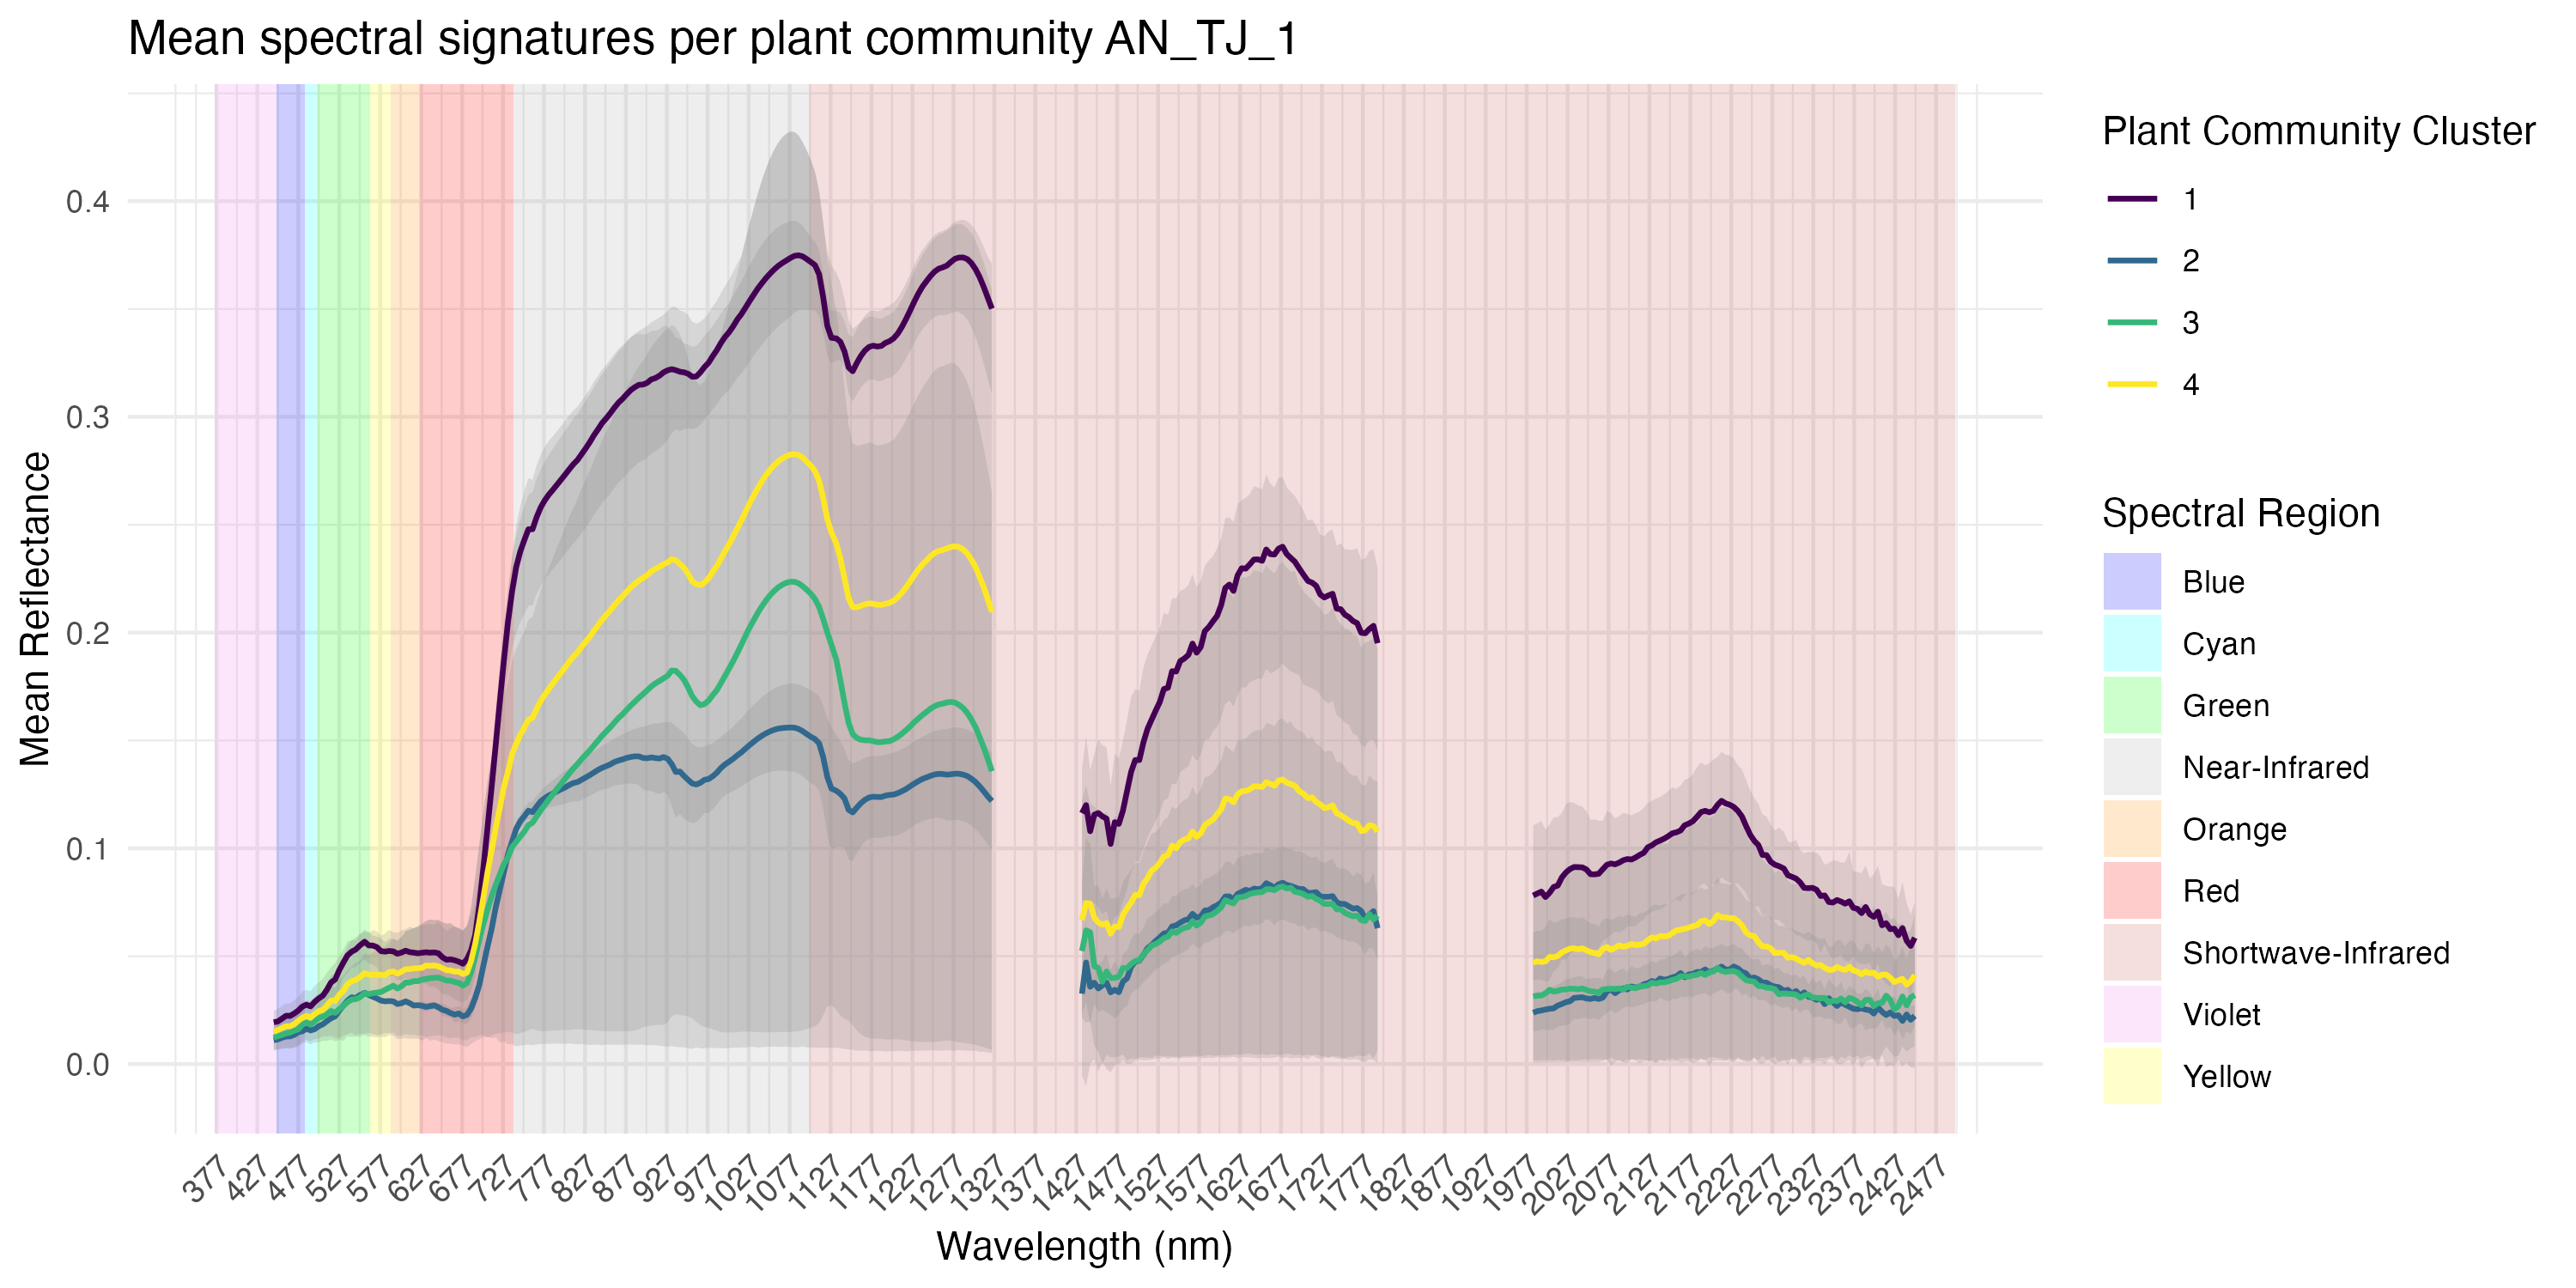
\includegraphics[width=\textwidth]{Figures/spectral_signatures/AN_TJ_1_mean_signature_plot_plant_community.png}
    \caption{}
    \label{fig:mss_pc_antj1}
  \end{subfigure}

  \caption{Spectral signature plot \ref{fig:ss_pc_antj1} and mean spectral signature plot \ref{fig:mss_pc_antj1} grouped by plant community cluster for test site AN\_TJ\_1}
  \label{fig:group_pc_ht_antj1}
\end{figure}

\subsection{AN\_TJ\_2}

\begin{figure}[H]
  \centering

  \begin{subfigure}[b]{0.49\textwidth}
    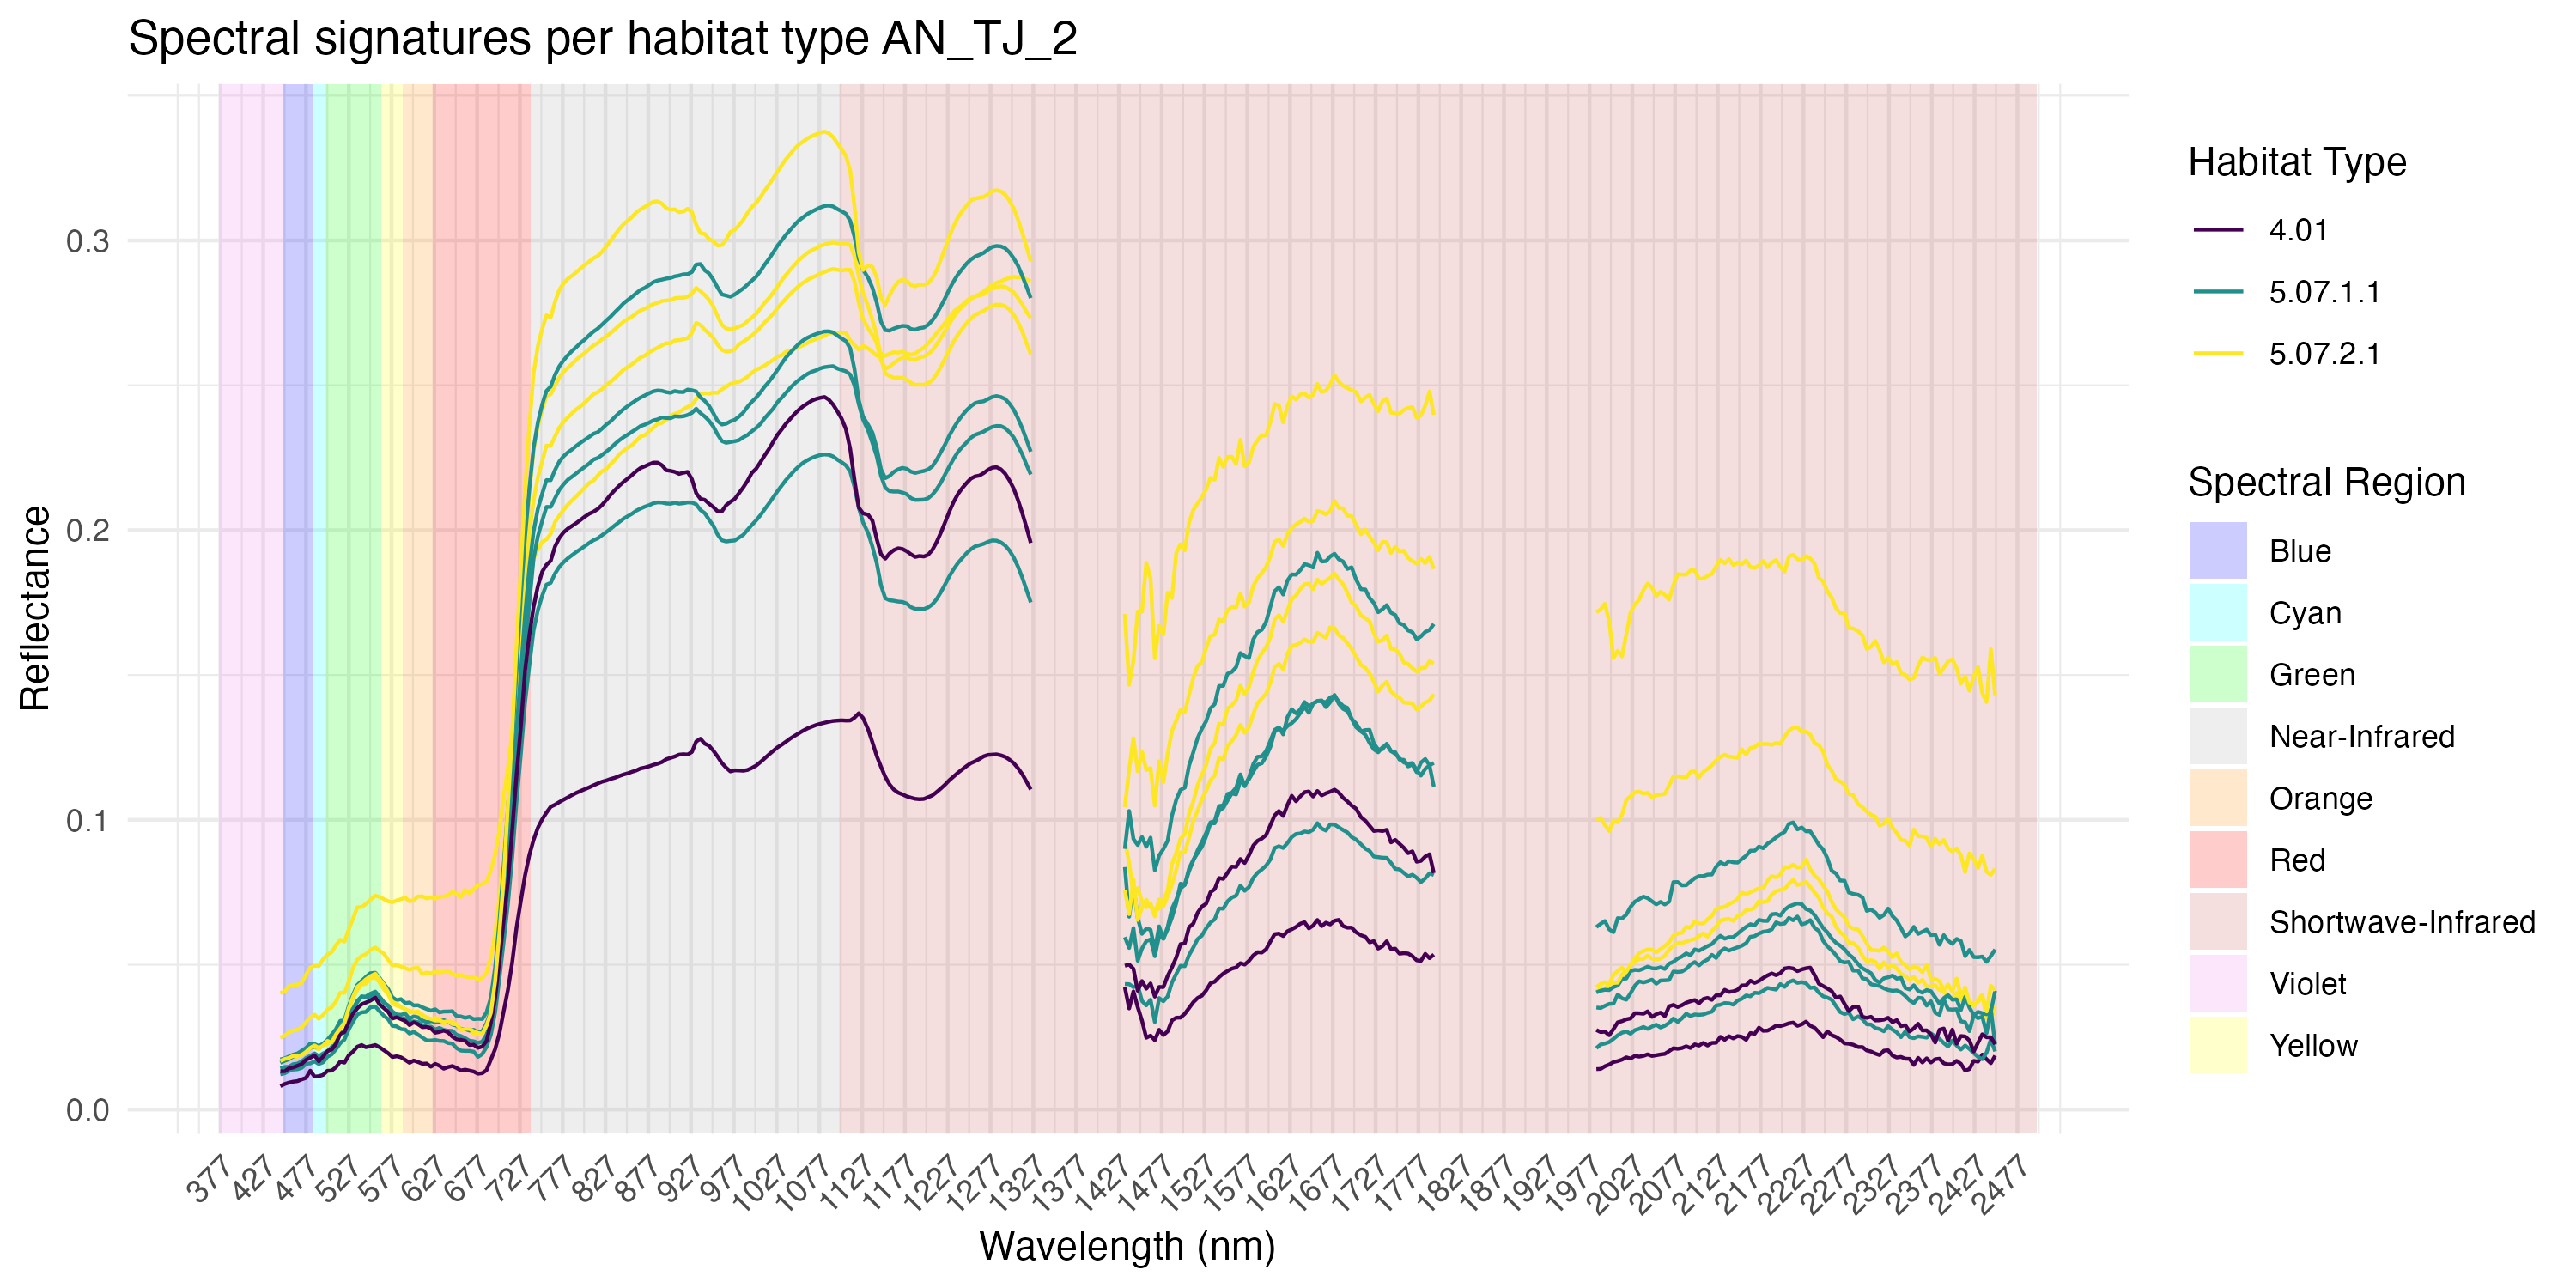
\includegraphics[width=\textwidth]{Figures/spectral_signatures/AN_TJ_2_signature_plot_habitat.png}
    \caption{}
    \label{fig:ss_ht_antj2}
  \end{subfigure}
  \hfill
  \begin{subfigure}[b]{0.49\textwidth}
    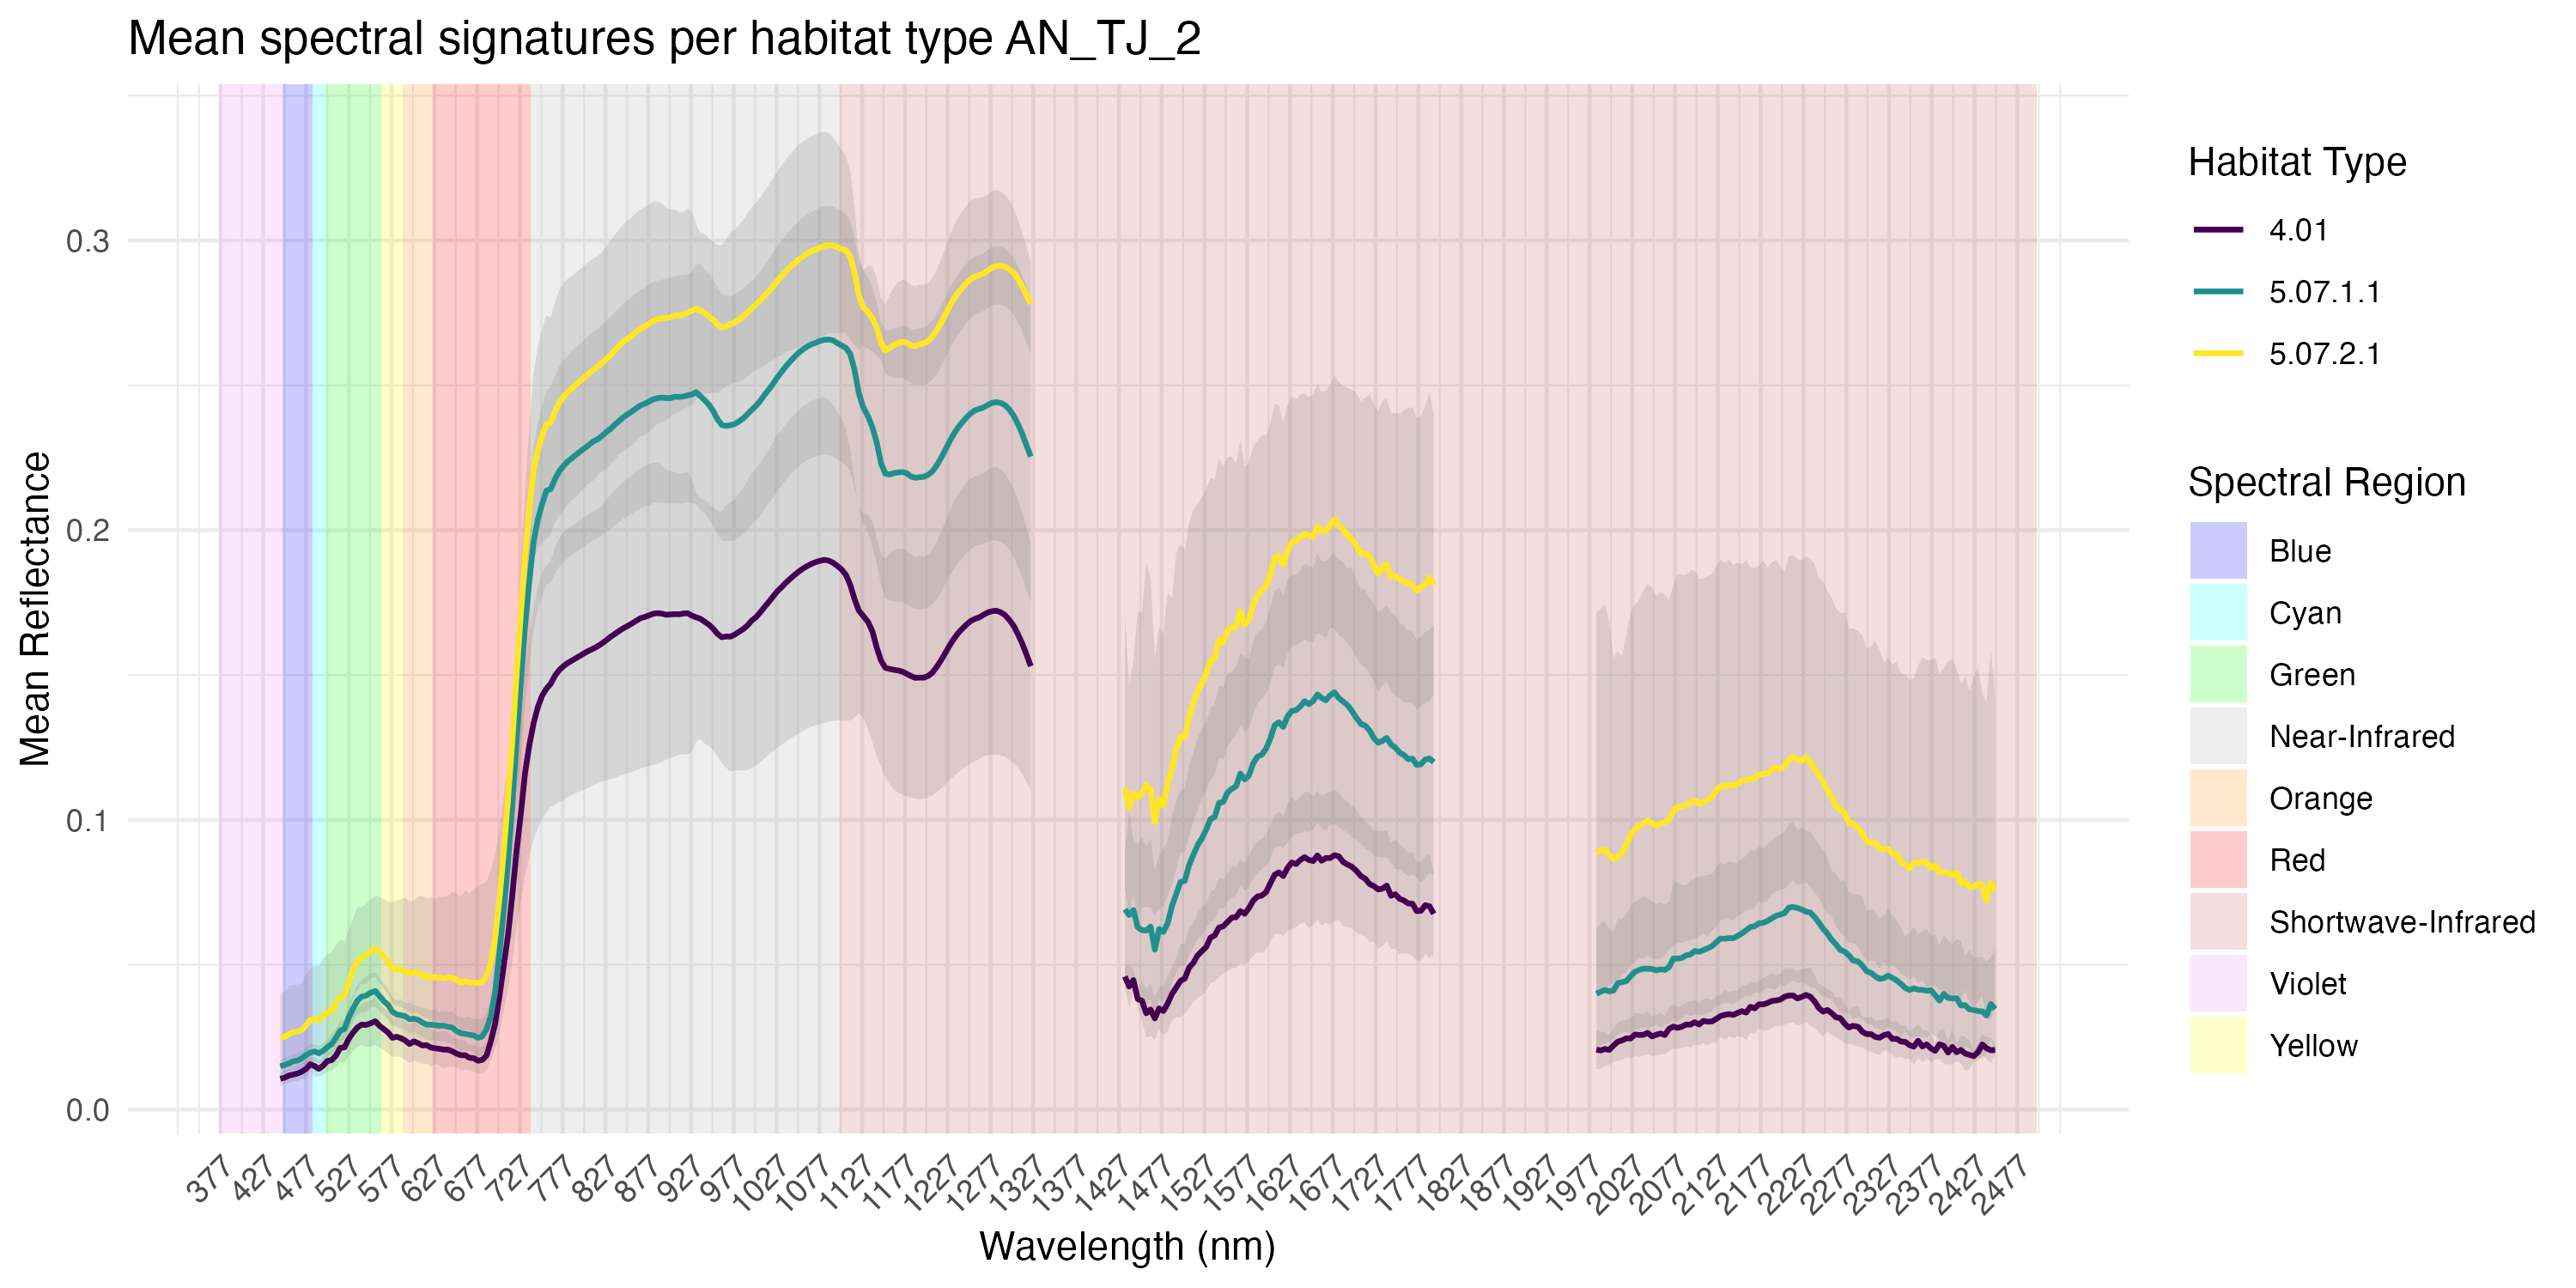
\includegraphics[width=\textwidth]{Figures/spectral_signatures/AN_TJ_2_mean_signature_plot_habitat.png}
    \caption{}
    \label{fig:mss_ht_antj2}
  \end{subfigure}

  \caption{Spectral signature plot \ref{fig:ss_ht_antj2} and mean spectral signature plot \ref{fig:mss_ht_antj2} grouped by habitat type for test site AN\_TJ\_2}
  \label{fig:group_ss_ht_antj2}
\end{figure}

\begin{figure}[H]
  \centering

  \begin{subfigure}[b]{0.49\textwidth}
    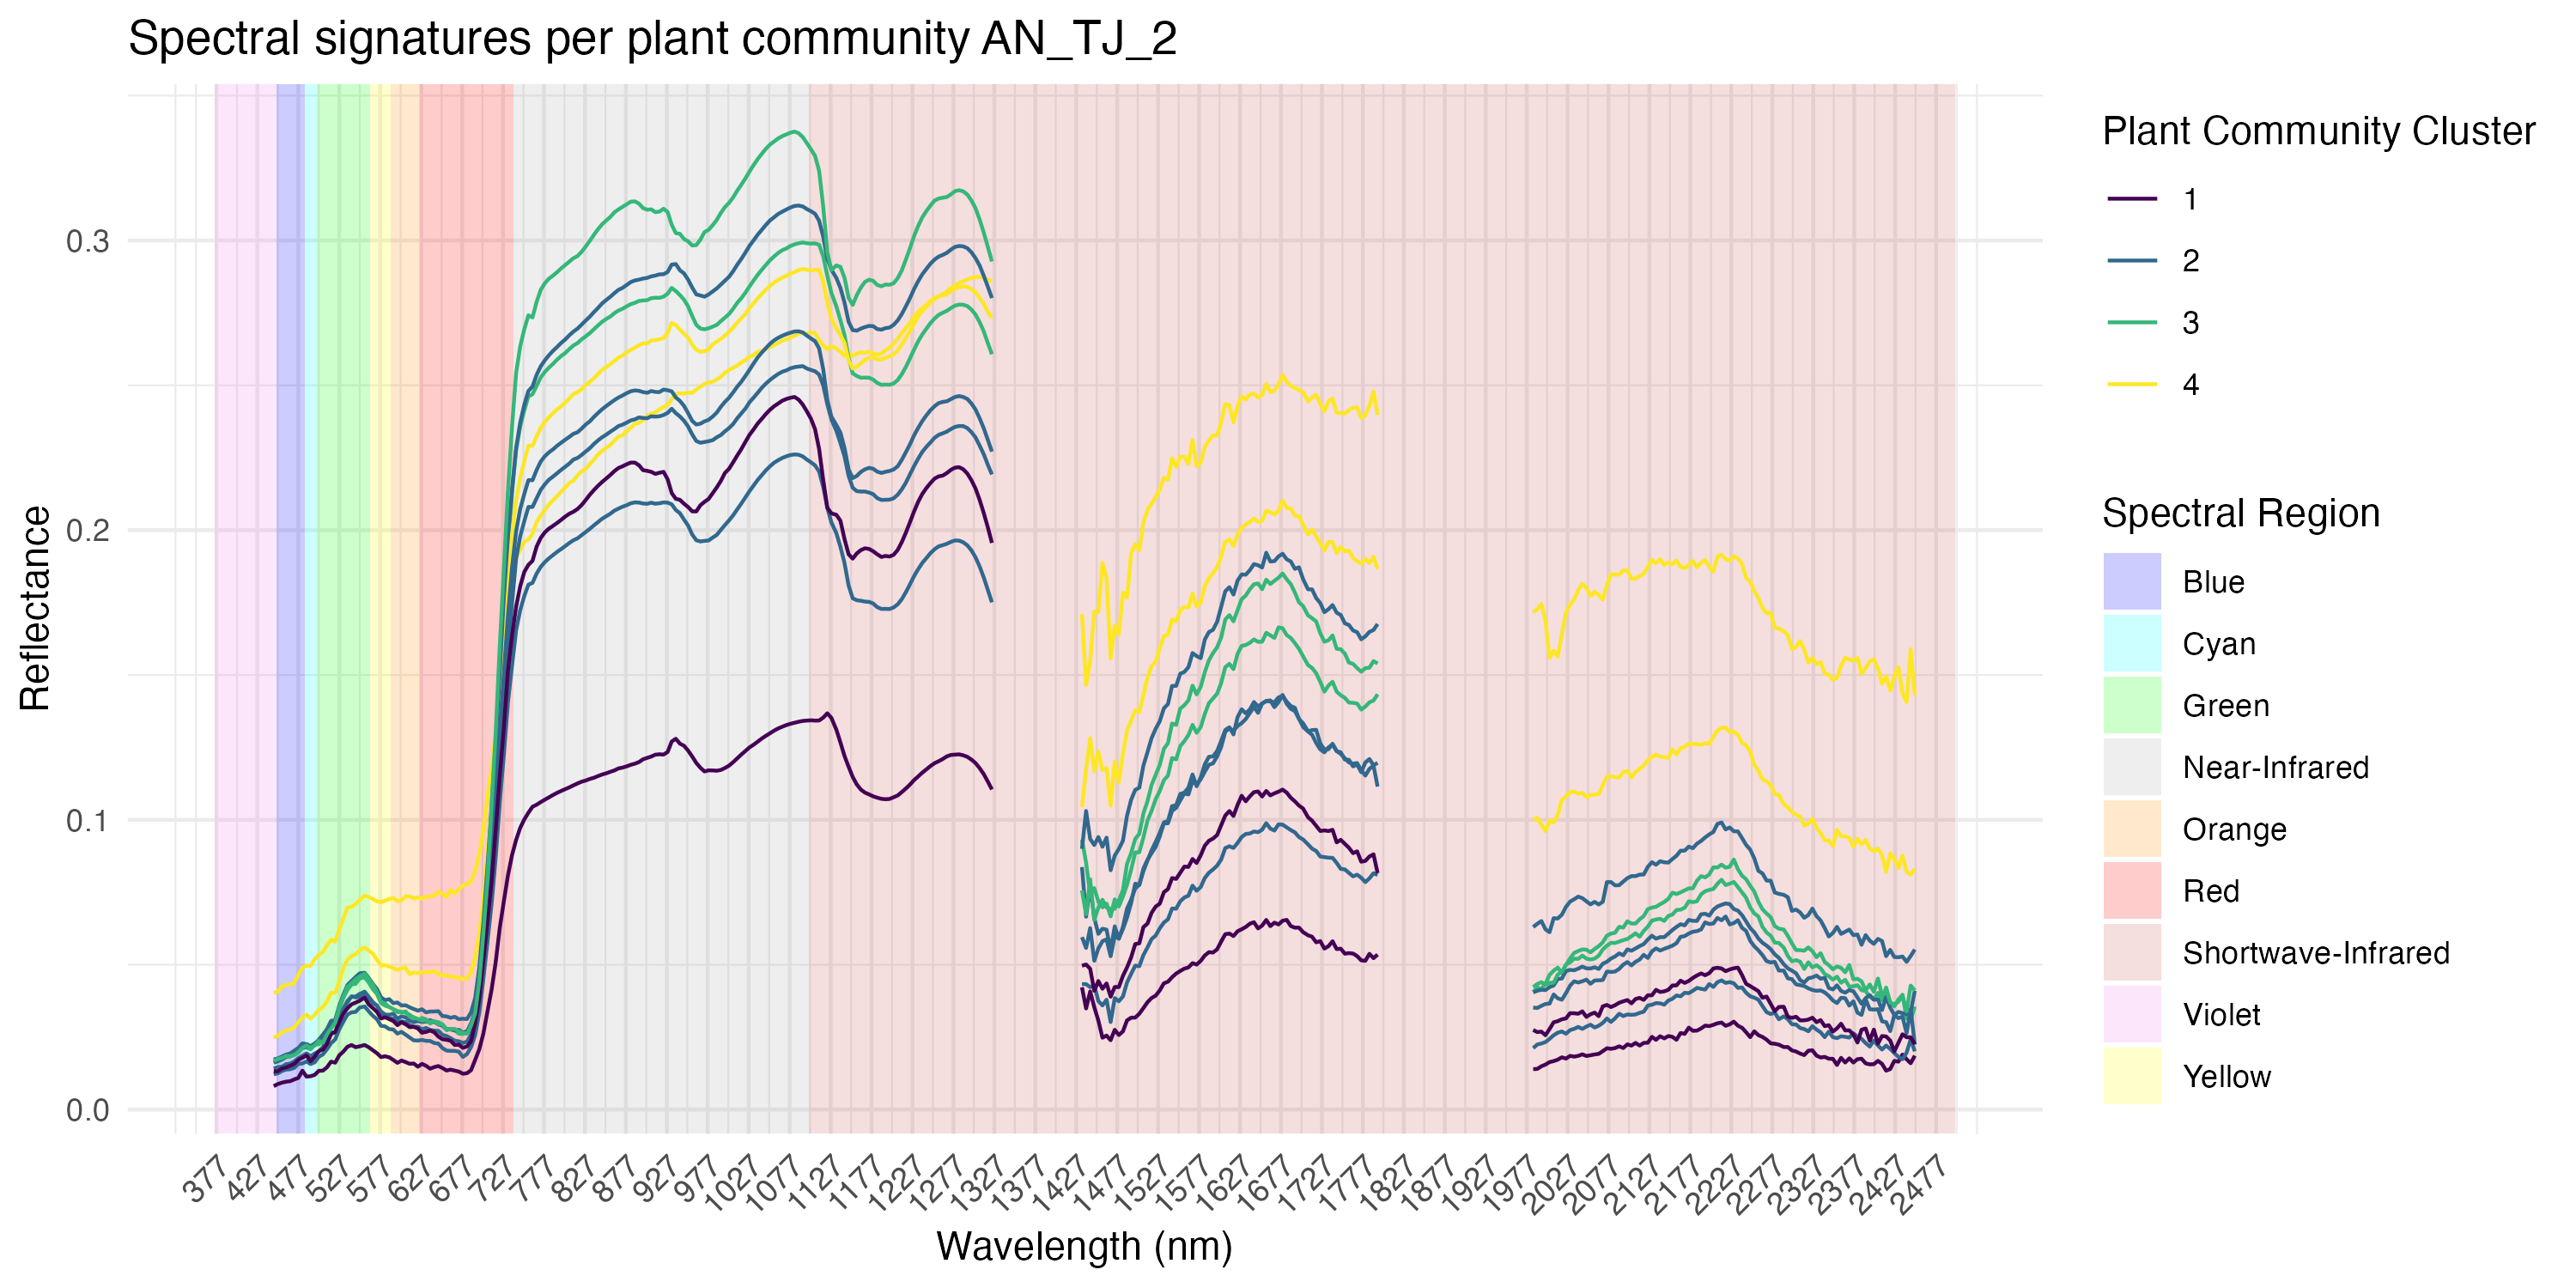
\includegraphics[width=\textwidth]{Figures/spectral_signatures/AN_TJ_2_signature_plot_plant_community.png}
    \caption{}
    \label{fig:ss_pc_antj2}
  \end{subfigure}
  \hfill
  \begin{subfigure}[b]{0.49\textwidth}
    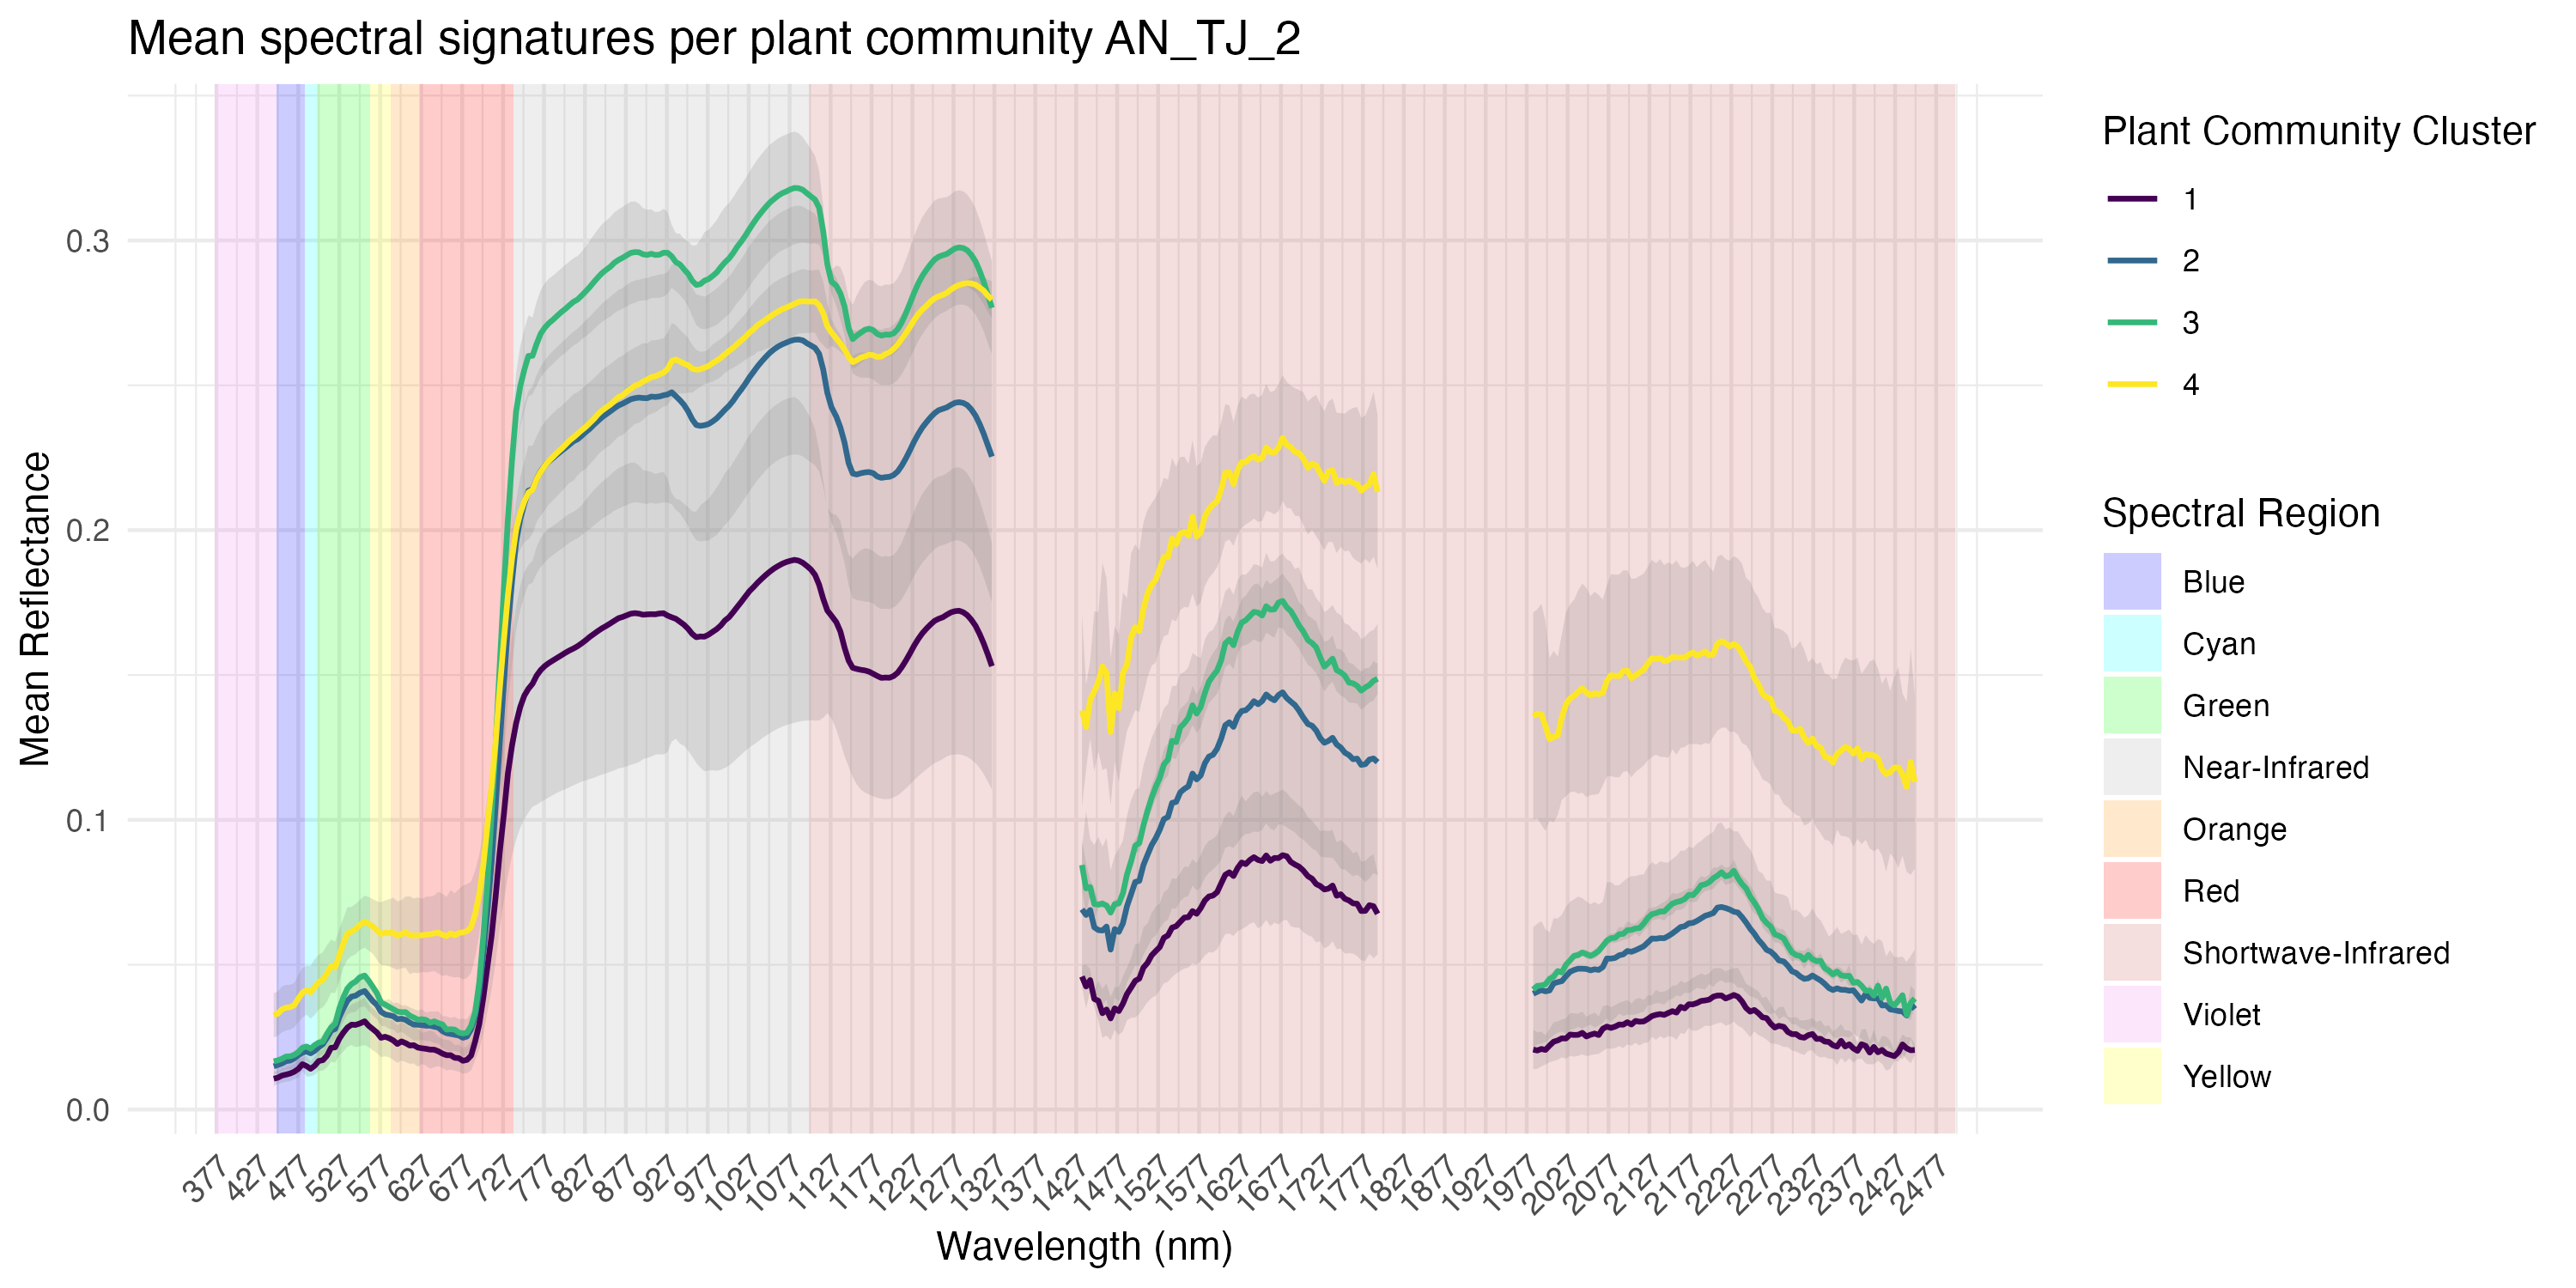
\includegraphics[width=\textwidth]{Figures/spectral_signatures/AN_TJ_2_mean_signature_plot_plant_community.png}
    \caption{}
    \label{fig:mss_pc_antj2}
  \end{subfigure}

  \caption{Spectral signature plot \ref{fig:ss_pc_antj2} and mean spectral signature plot \ref{fig:mss_pc_antj2} grouped by plant community cluster for test site AN\_TJ\_2}
  \label{fig:group_pc_ht_antj2}
\end{figure}

\subsection{ATQ\_VK\_1}

\begin{figure}[H]
  \centering

  \begin{subfigure}[b]{0.49\textwidth}
    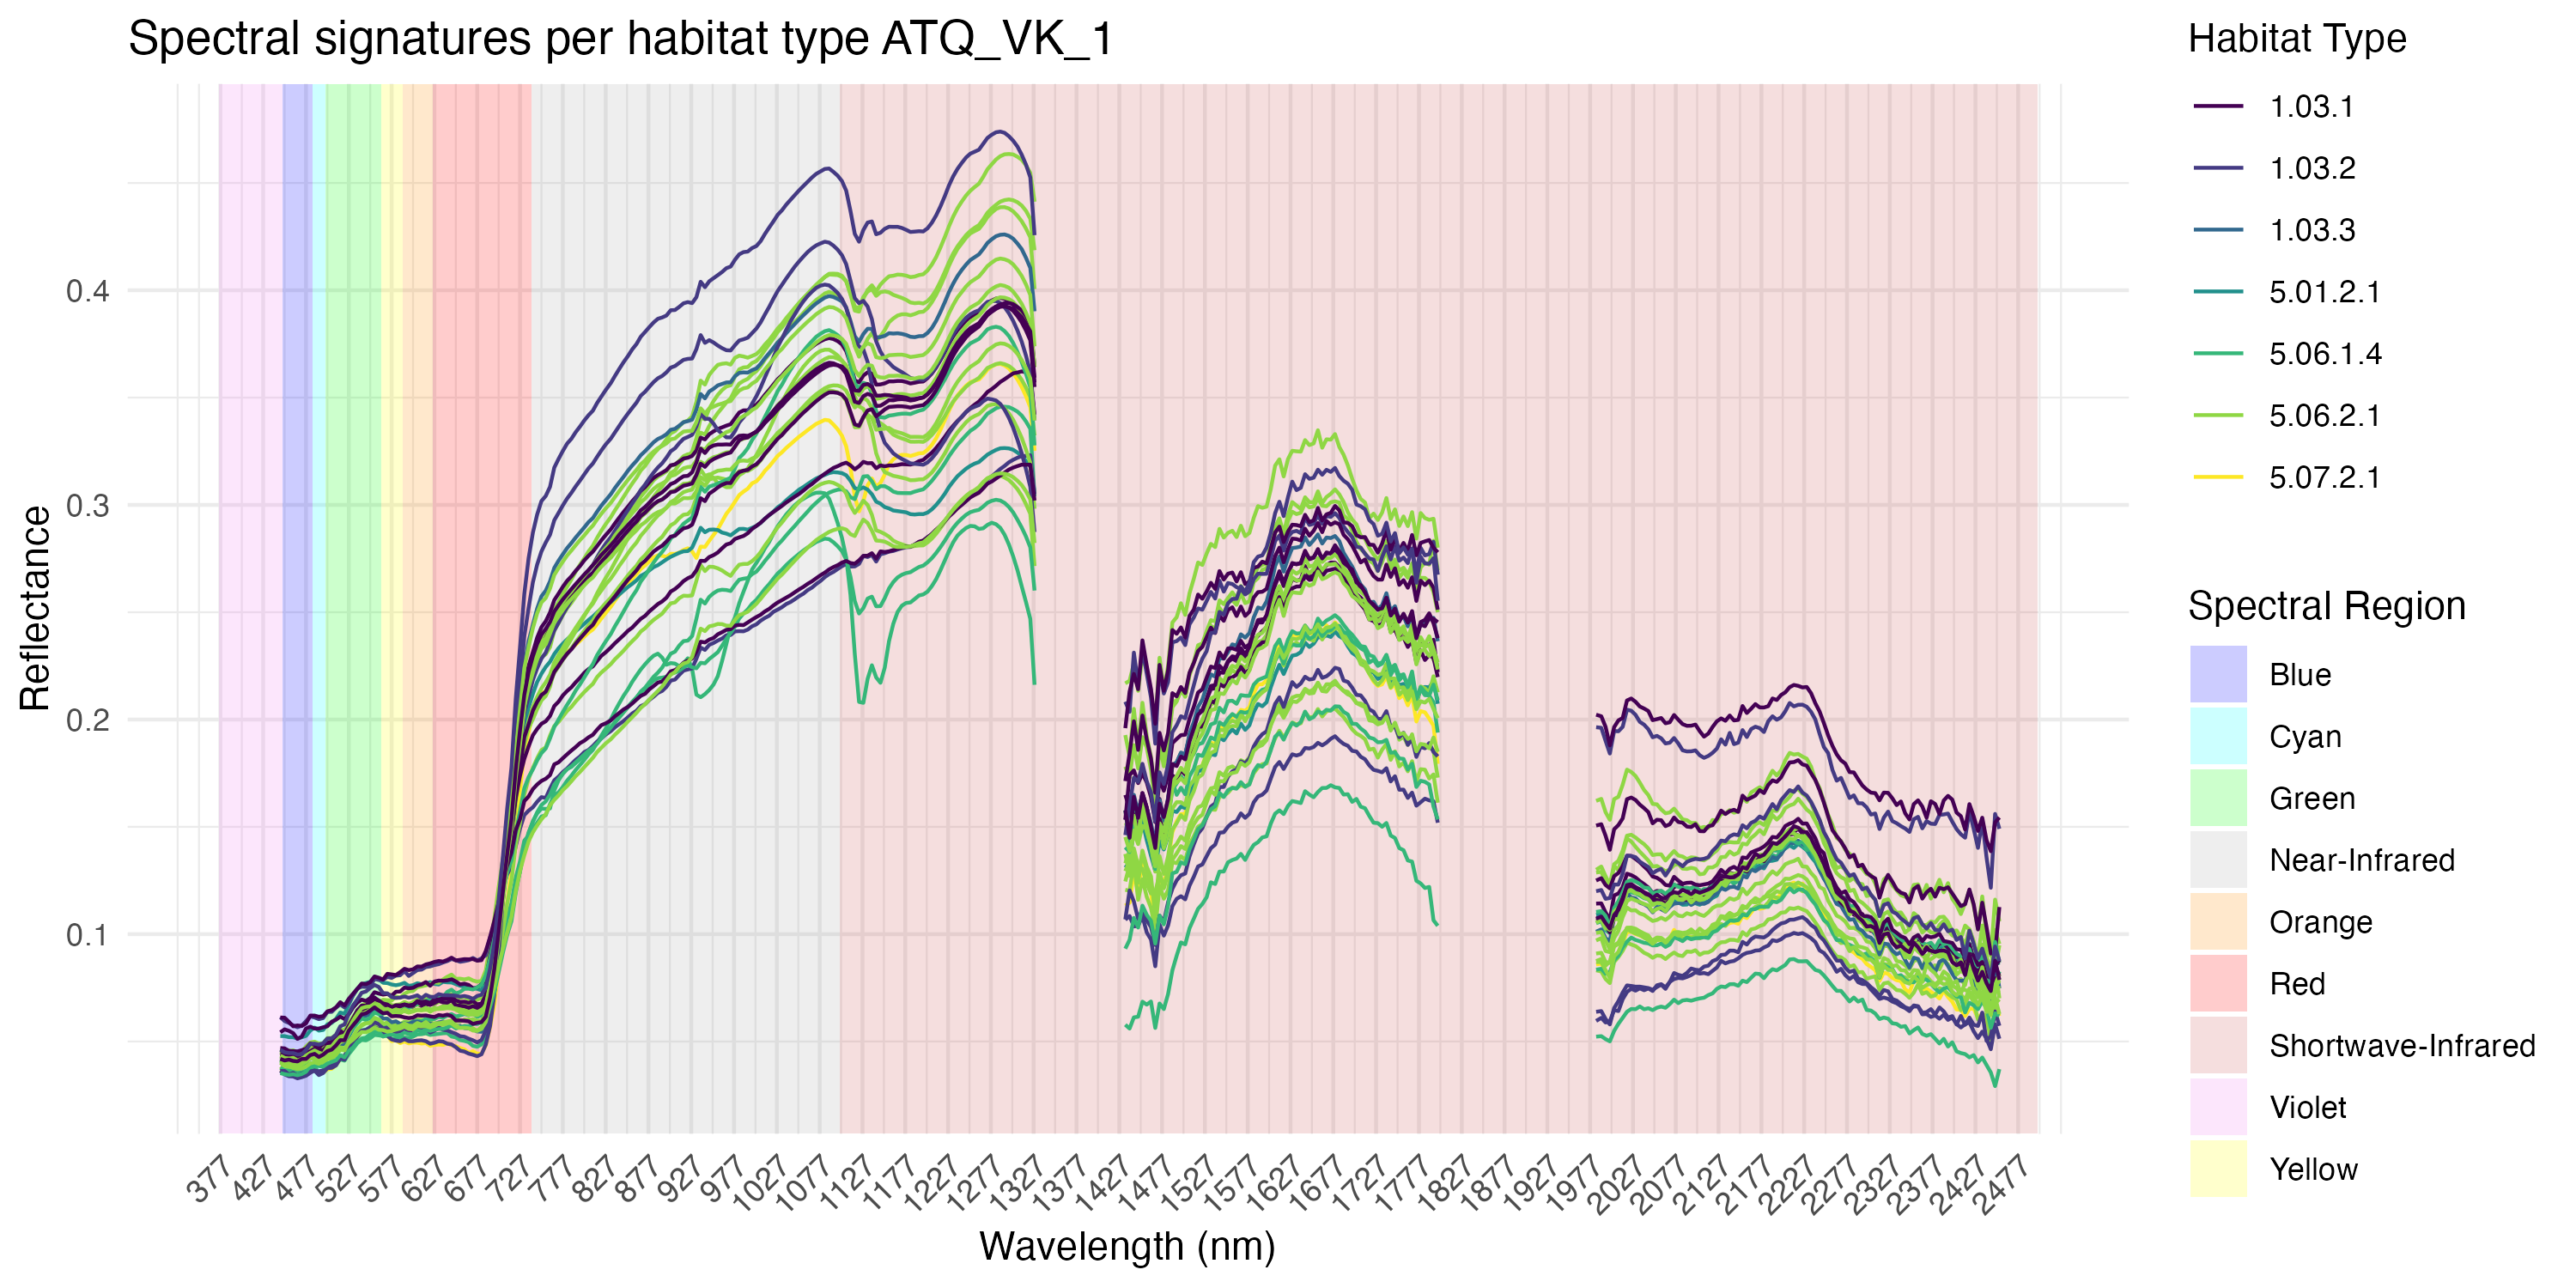
\includegraphics[width=\textwidth]{Figures/spectral_signatures/ATQ_VK_1_signature_plot_habitat.png}
    \caption{}
    \label{fig:ss_ht_atqvk1}
  \end{subfigure}
  \hfill
  \begin{subfigure}[b]{0.49\textwidth}
    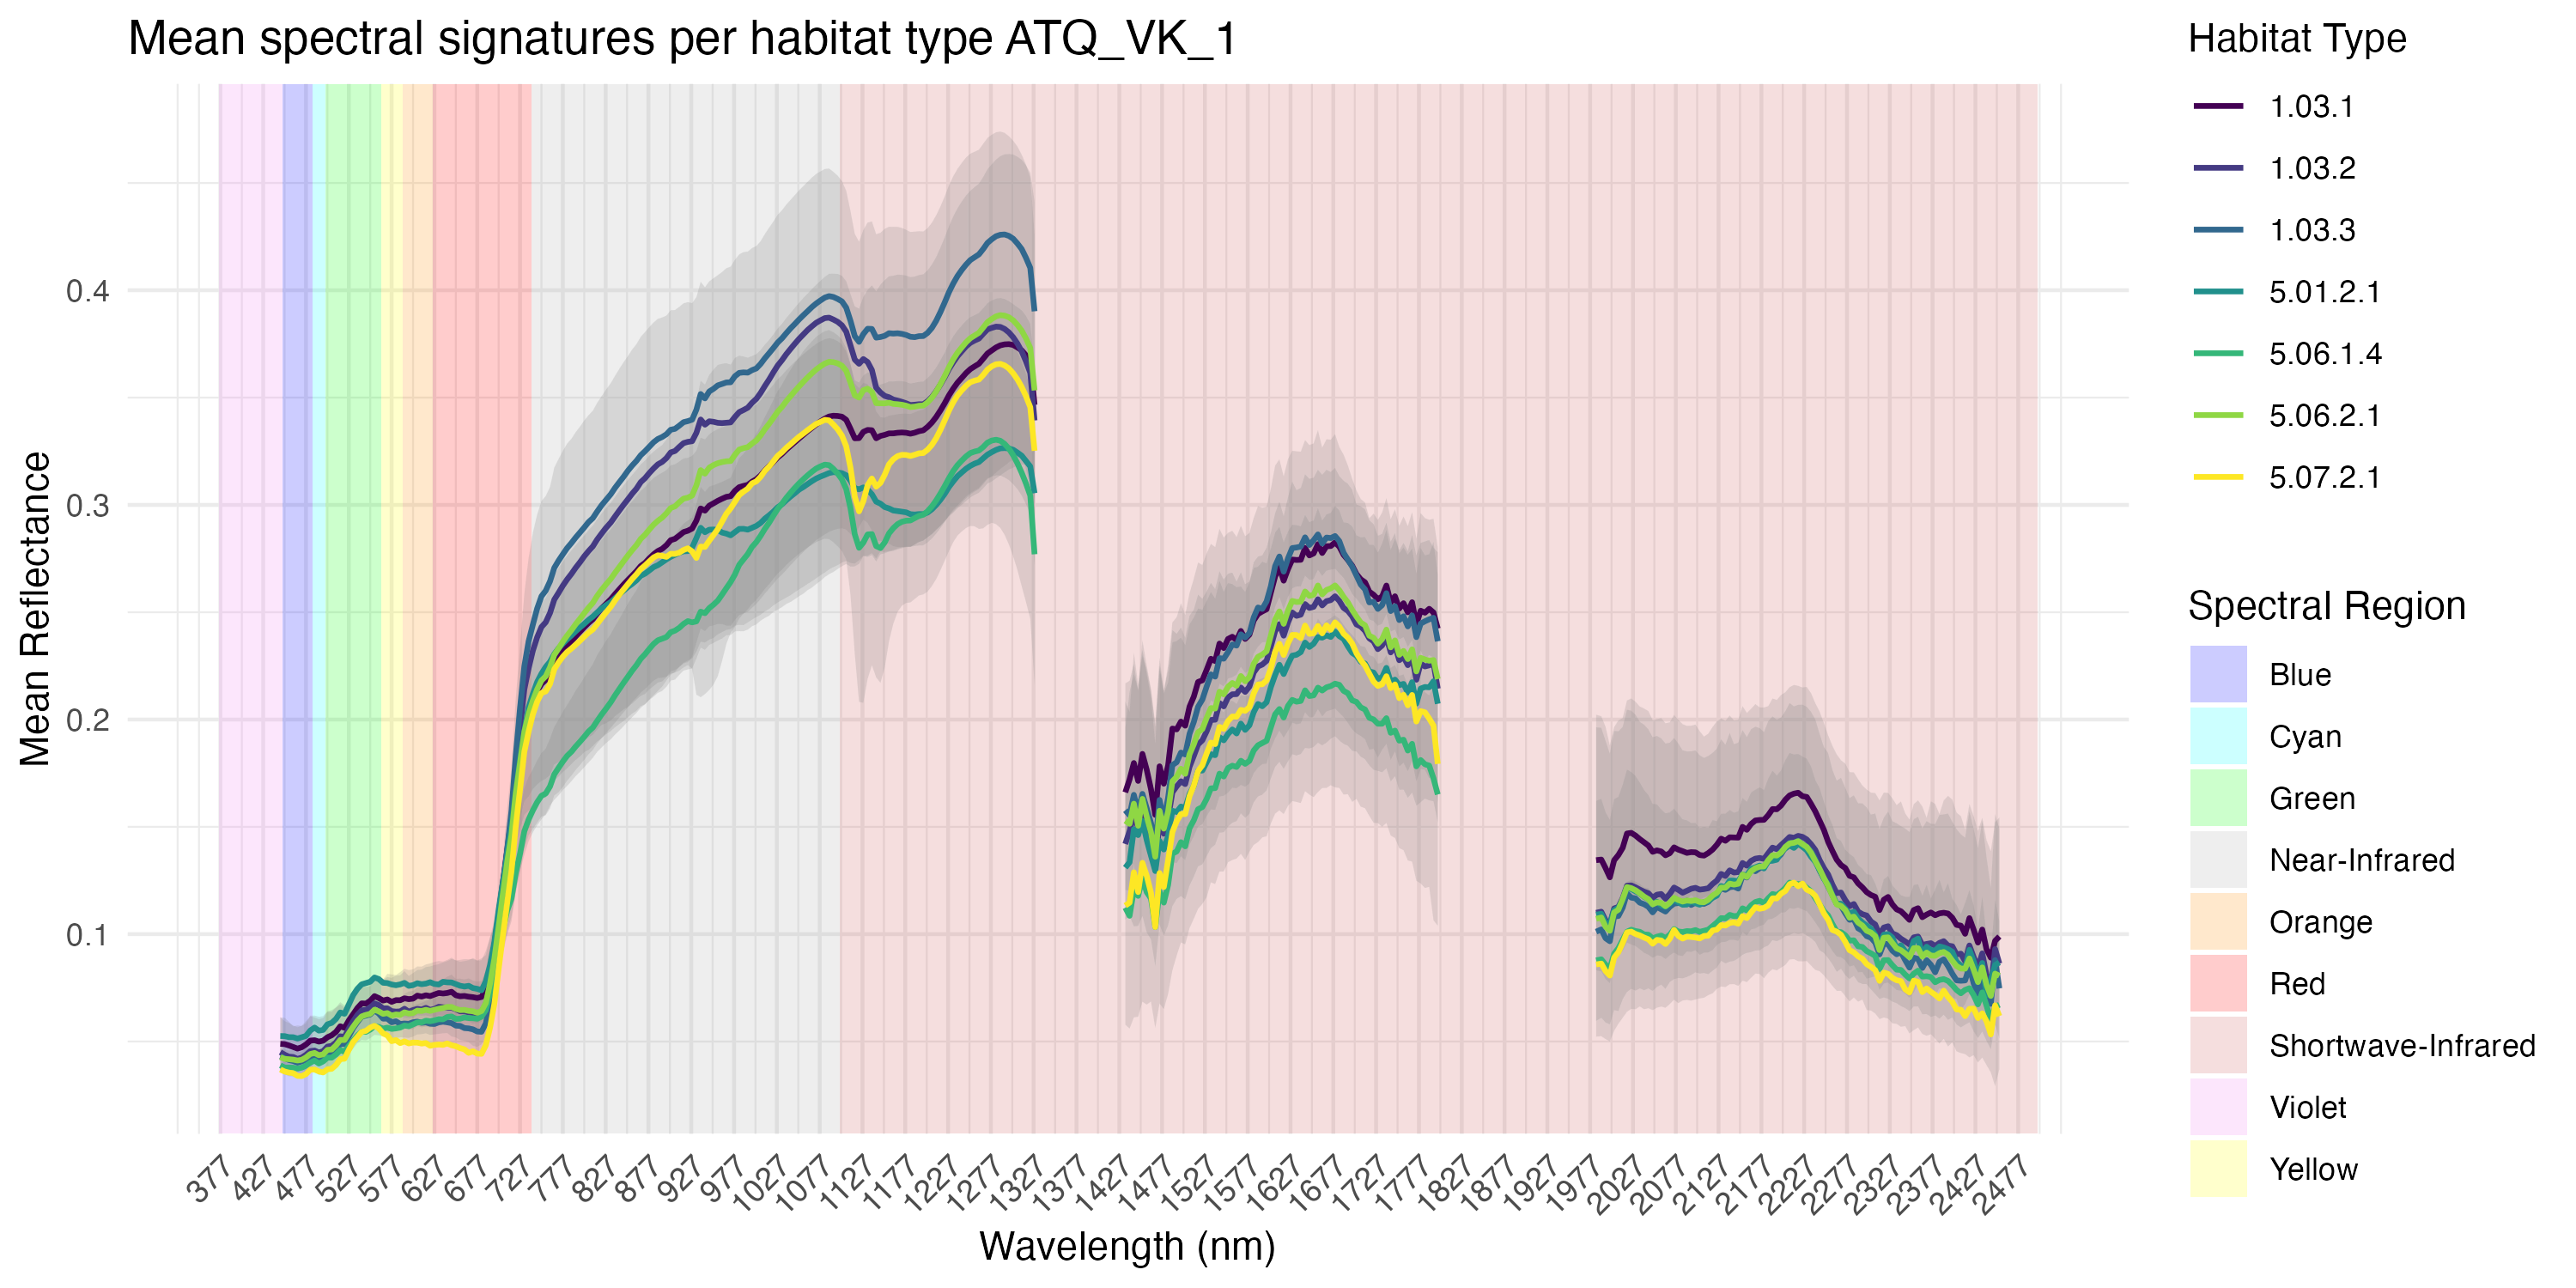
\includegraphics[width=\textwidth]{Figures/spectral_signatures/ATQ_VK_1_mean_signature_plot_habitat.png}
    \caption{}
    \label{fig:mss_ht_atqvk1}
  \end{subfigure}

  \caption{Spectral signature plot \ref{fig:ss_ht_atqvk1} and mean spectral signature plot \ref{fig:mss_ht_atqvk1} grouped by habitat type for test site ATQ\_VK\_1}
  \label{fig:group_ss_ht_atqvk1}
\end{figure}

\begin{figure}[H]
  \centering

  \begin{subfigure}[b]{0.49\textwidth}
    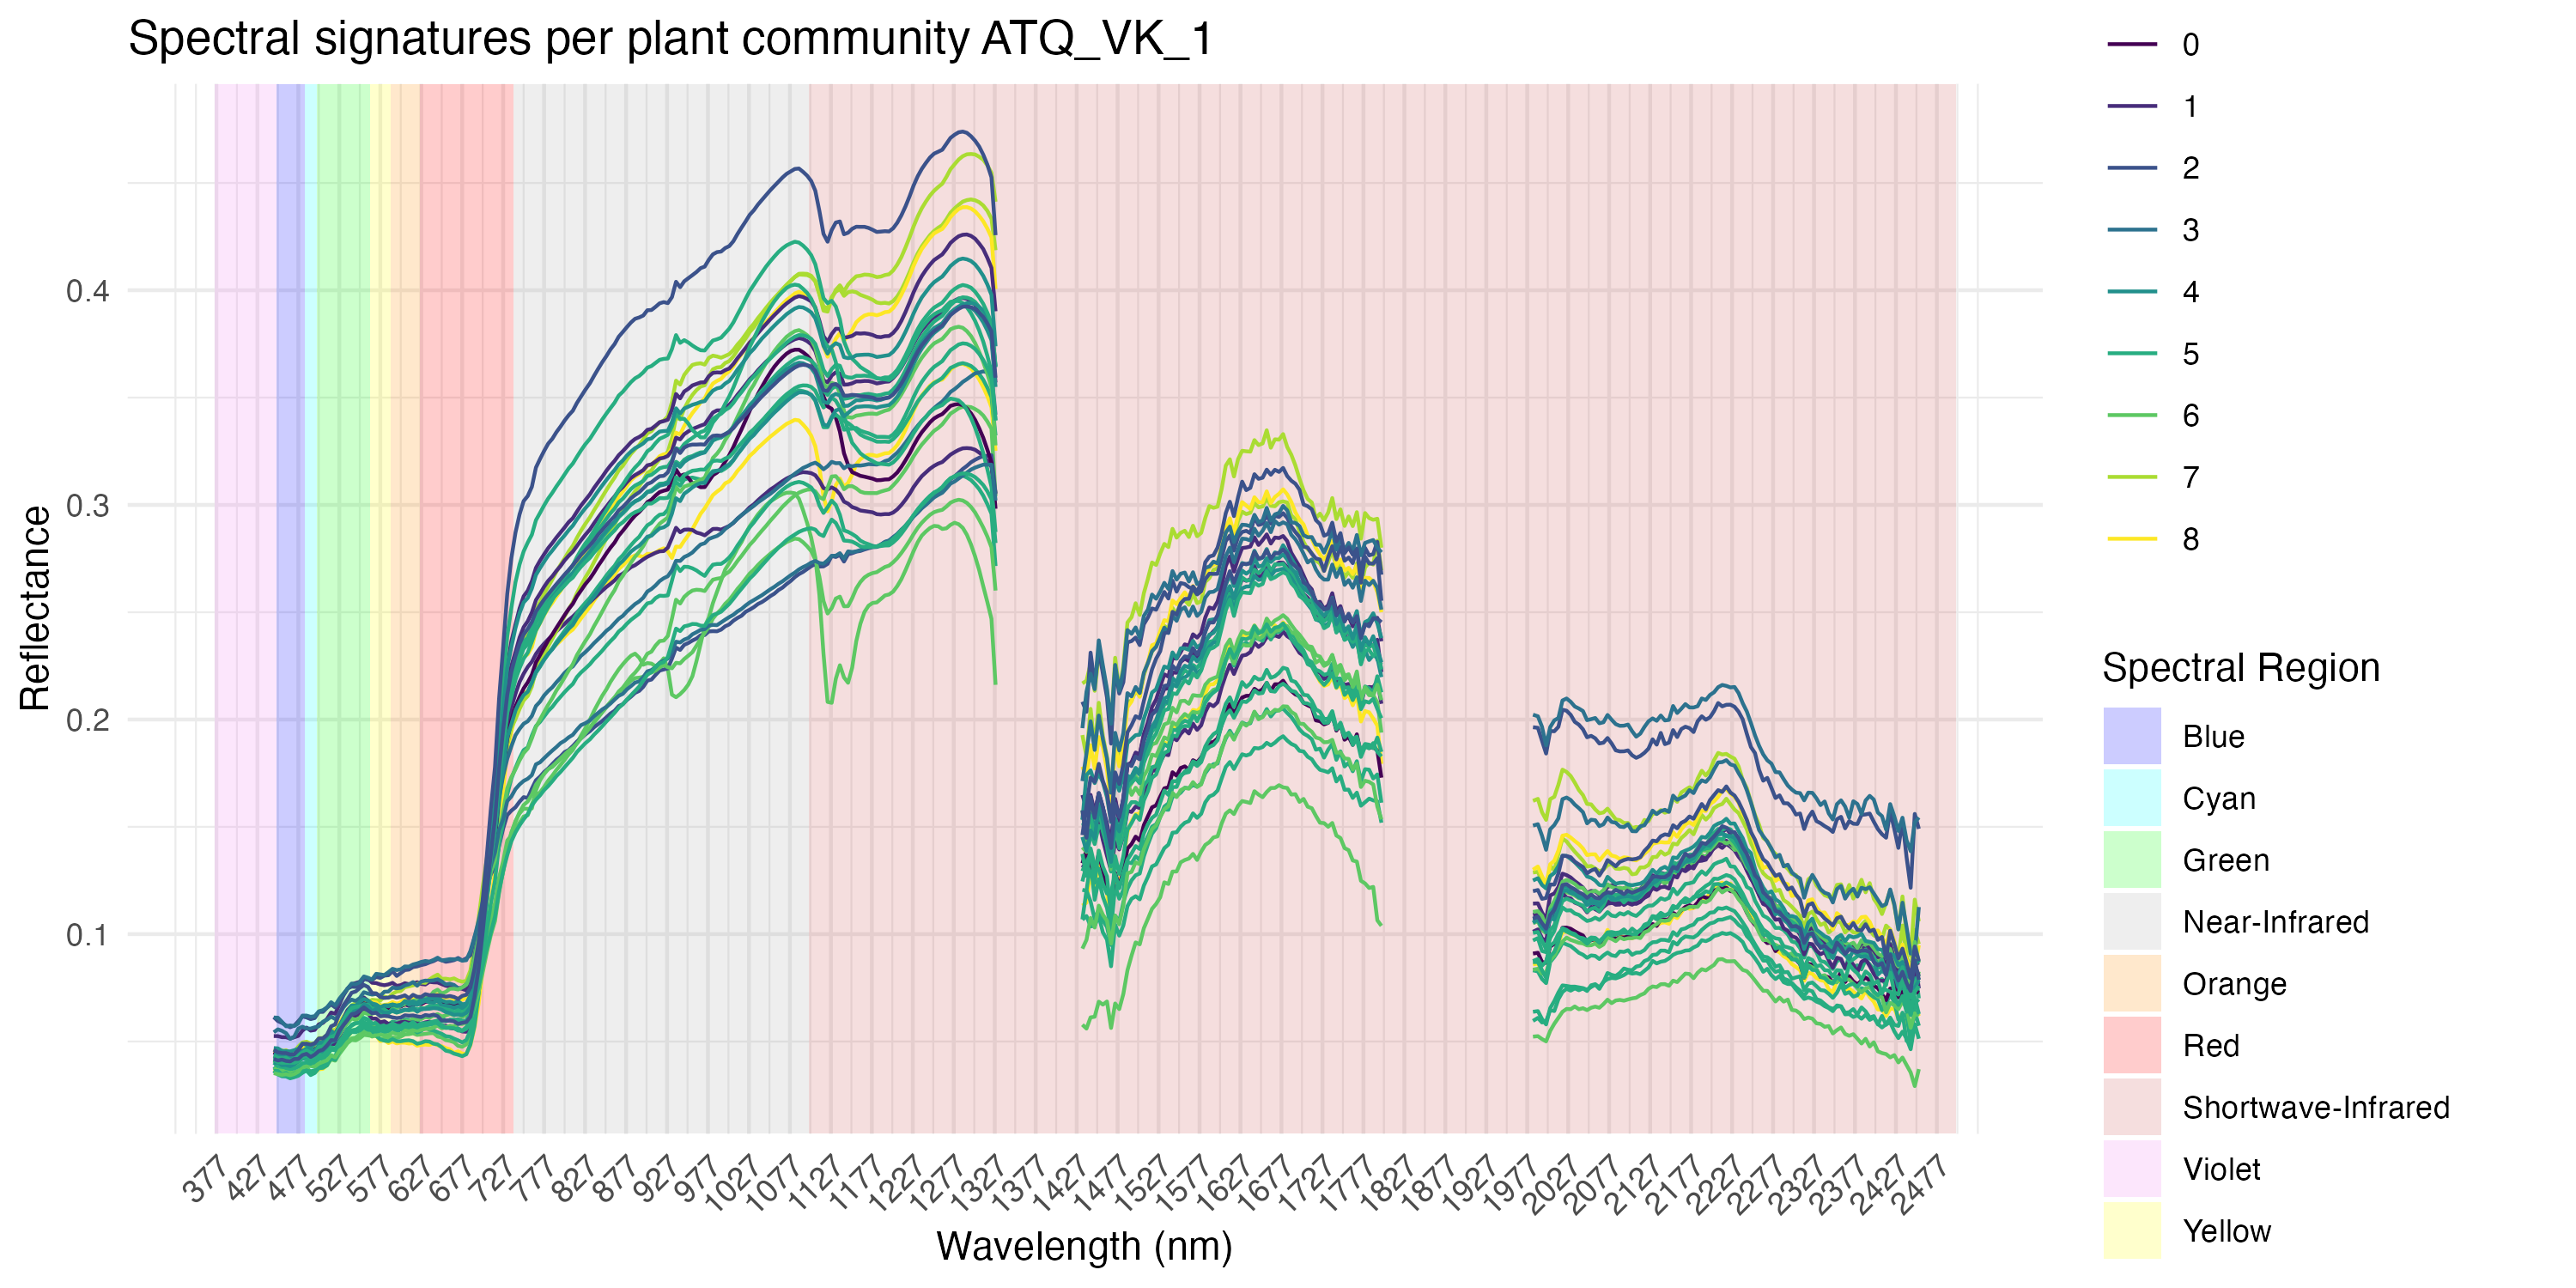
\includegraphics[width=\textwidth]{Figures/spectral_signatures/ATQ_VK_1_signature_plot_plant_community.png}
    \caption{}
    \label{fig:ss_pc_atqvk1}
  \end{subfigure}
  \hfill
  \begin{subfigure}[b]{0.49\textwidth}
    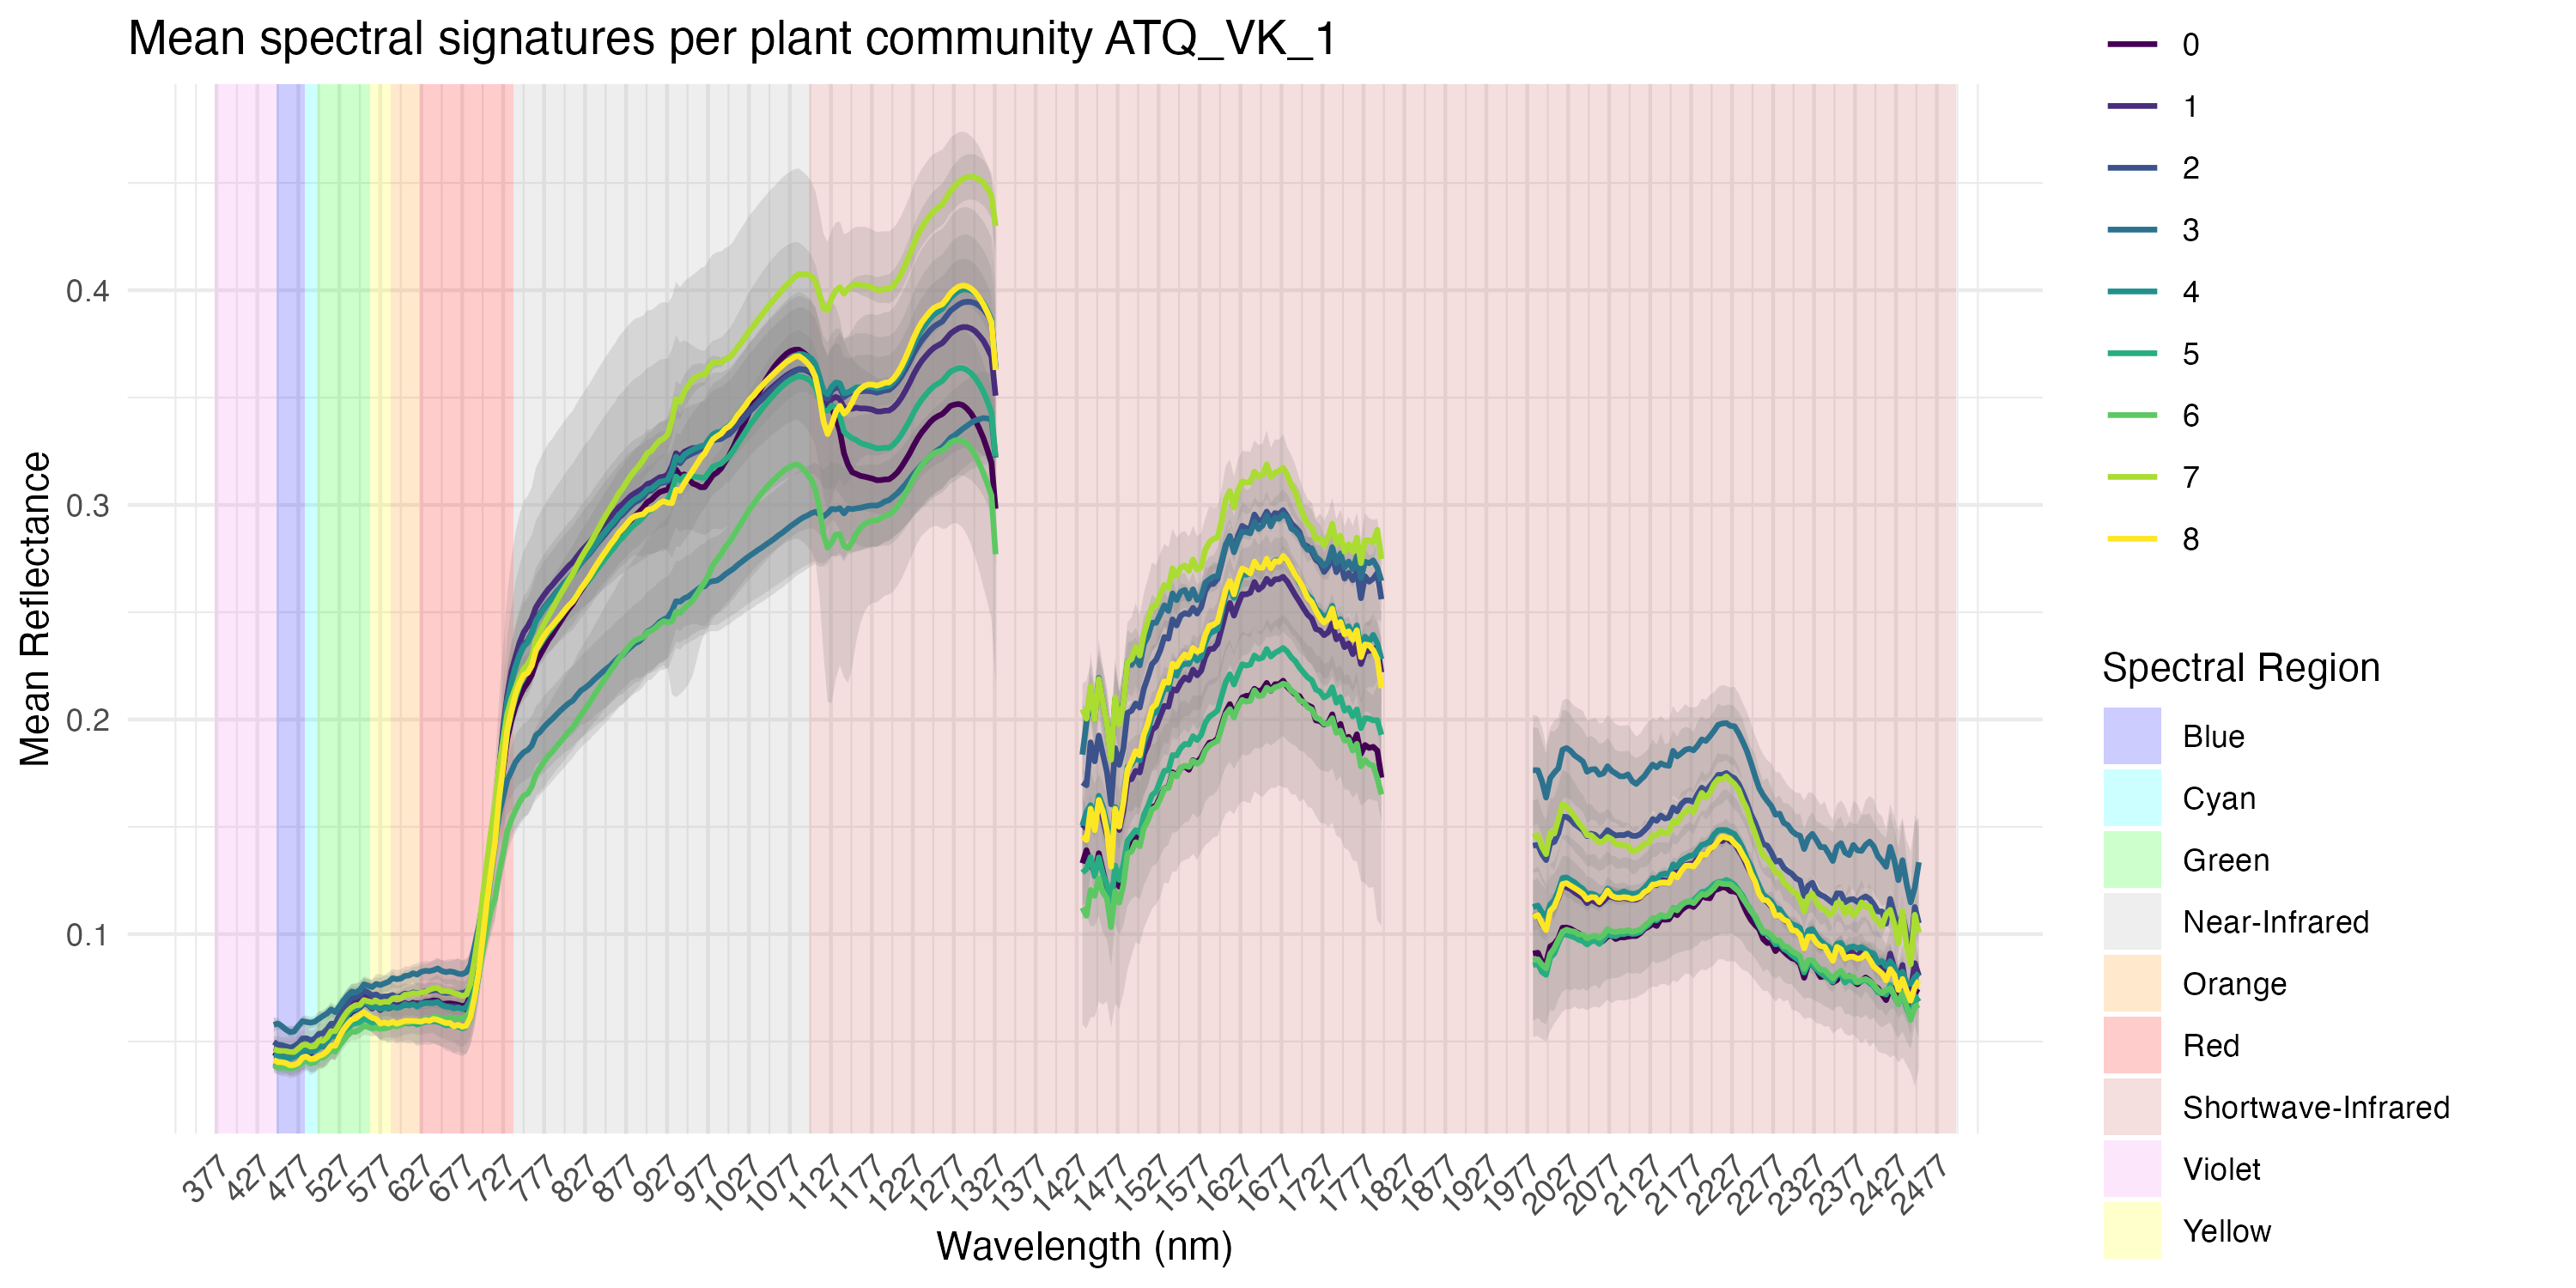
\includegraphics[width=\textwidth]{Figures/spectral_signatures/ATQ_VK_1_mean_signature_plot_plant_community.png}
    \caption{}
    \label{fig:mss_pc_atqvk1}
  \end{subfigure}

  \caption{Spectral signature plot \ref{fig:ss_pc_atqvk1} and mean spectral signature plot \ref{fig:mss_pc_atqvk1} grouped by plant community cluster for test site ATQ\_VK\_1}
  \label{fig:group_pc_ht_atqvk1}
\end{figure}

\subsection{BRW\_PW\_1}

\begin{figure}[H]
  \centering

  \begin{subfigure}[b]{0.49\textwidth}
    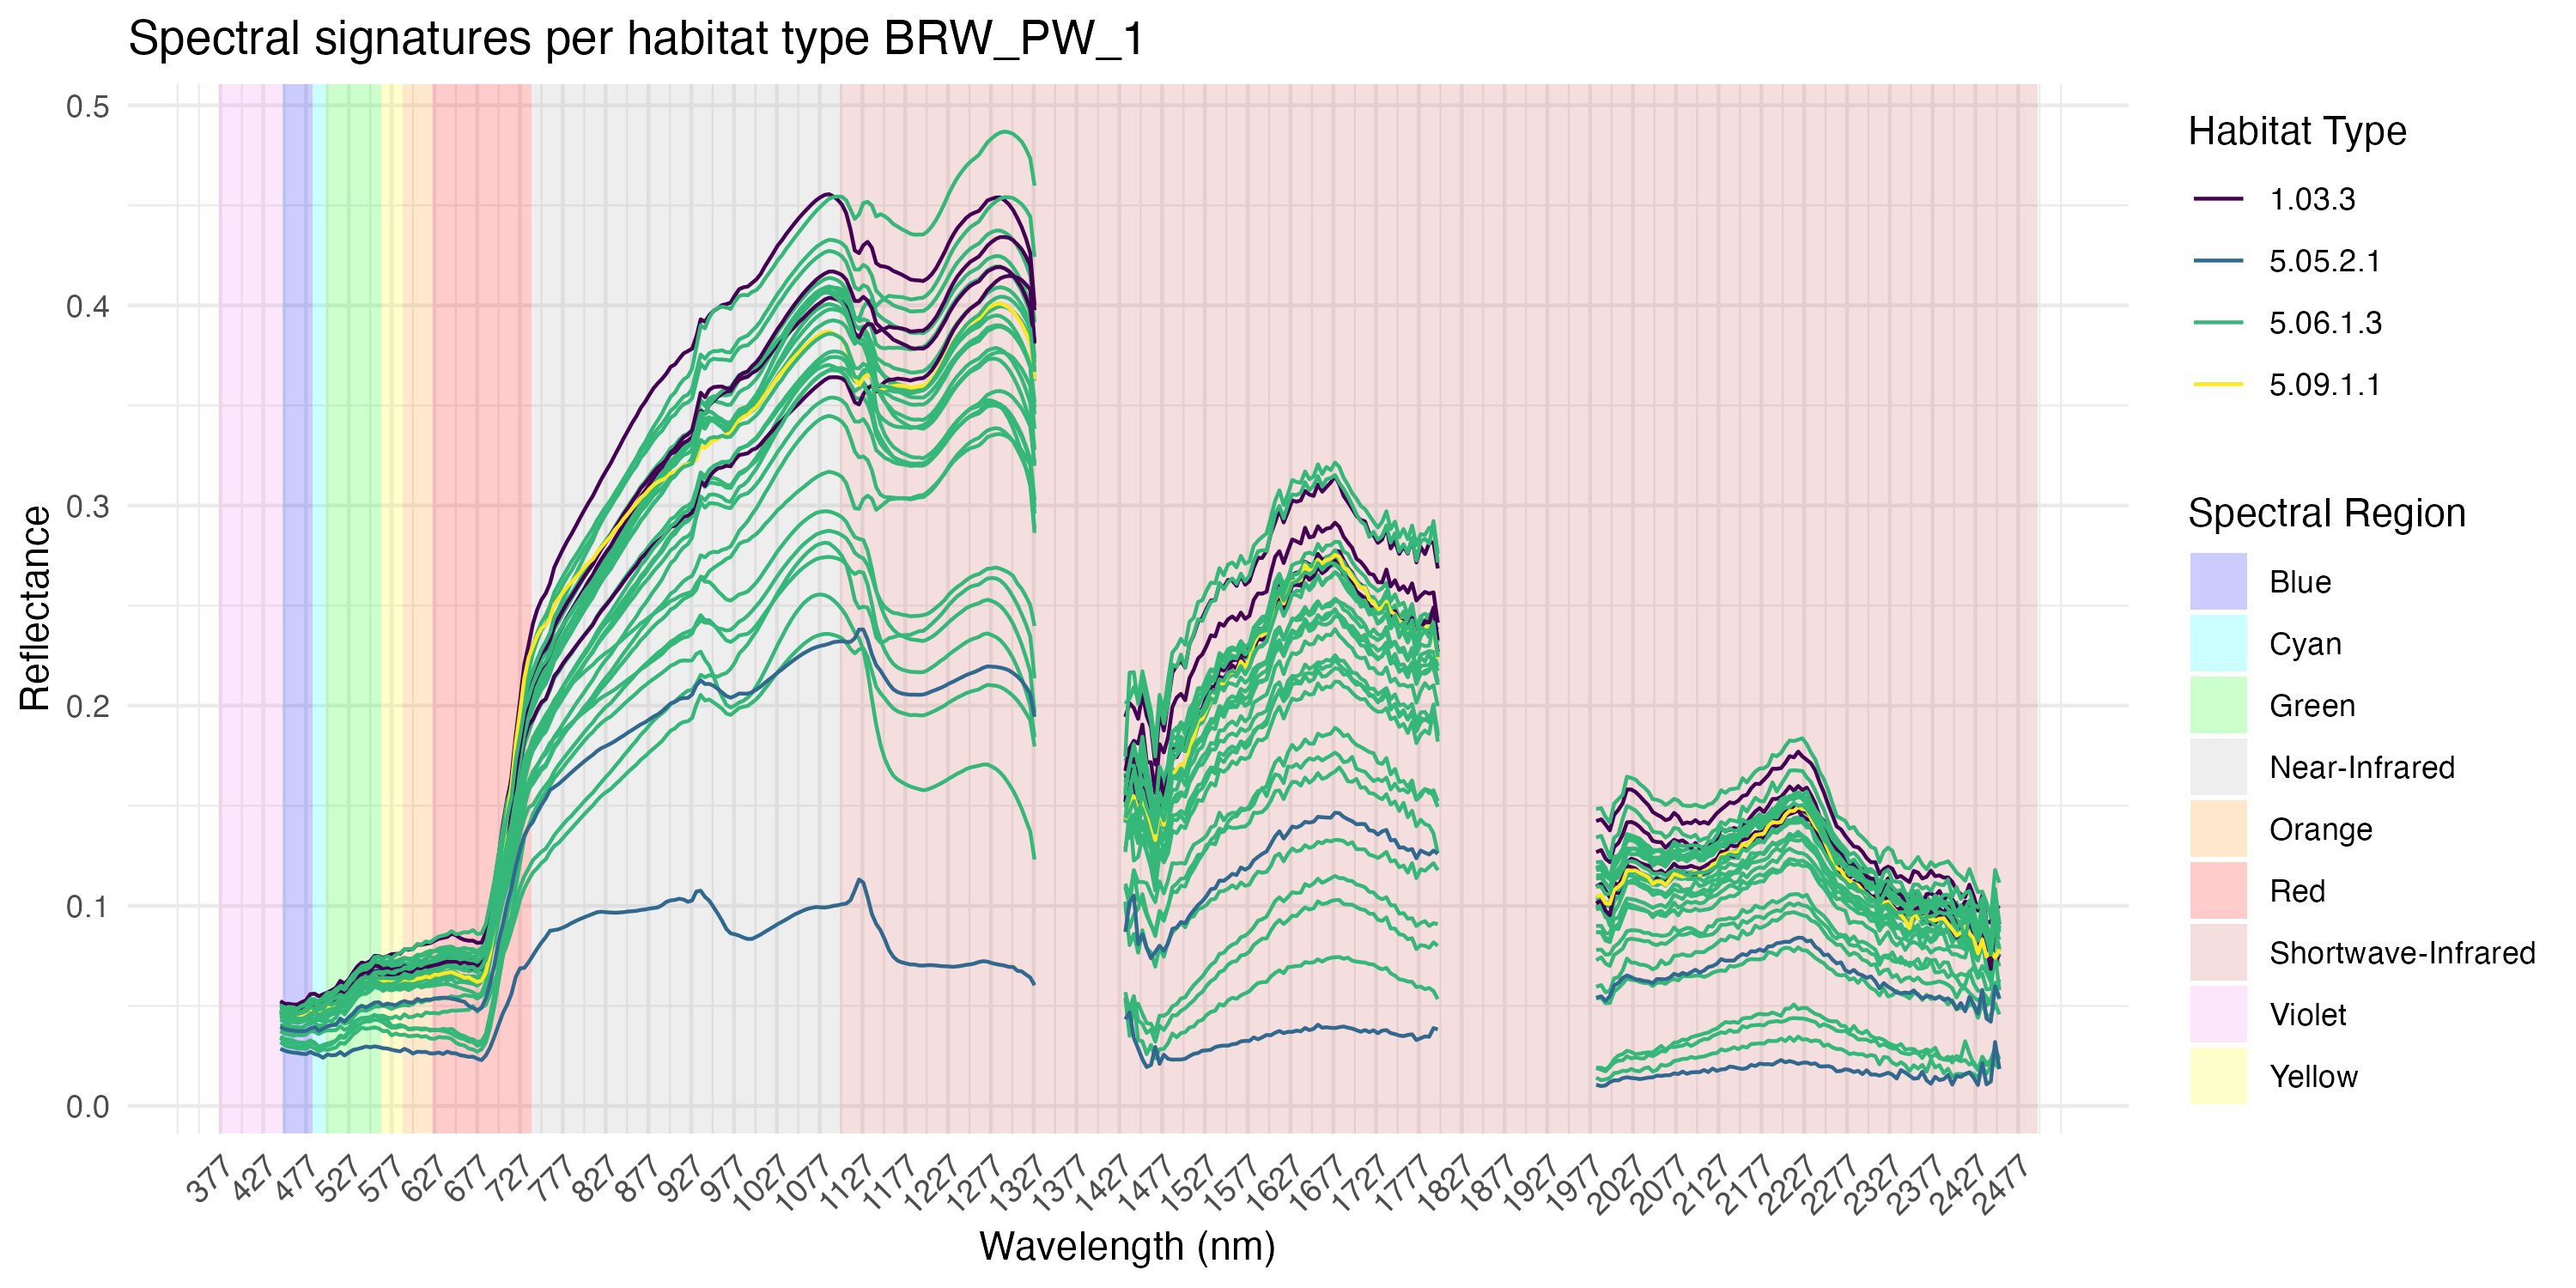
\includegraphics[width=\textwidth]{Figures/spectral_signatures/BRW_PW_1_signature_plot_habitat.png}
    \caption{}
    \label{fig:ss_ht_brwpw1}
  \end{subfigure}
  \hfill
  \begin{subfigure}[b]{0.49\textwidth}
    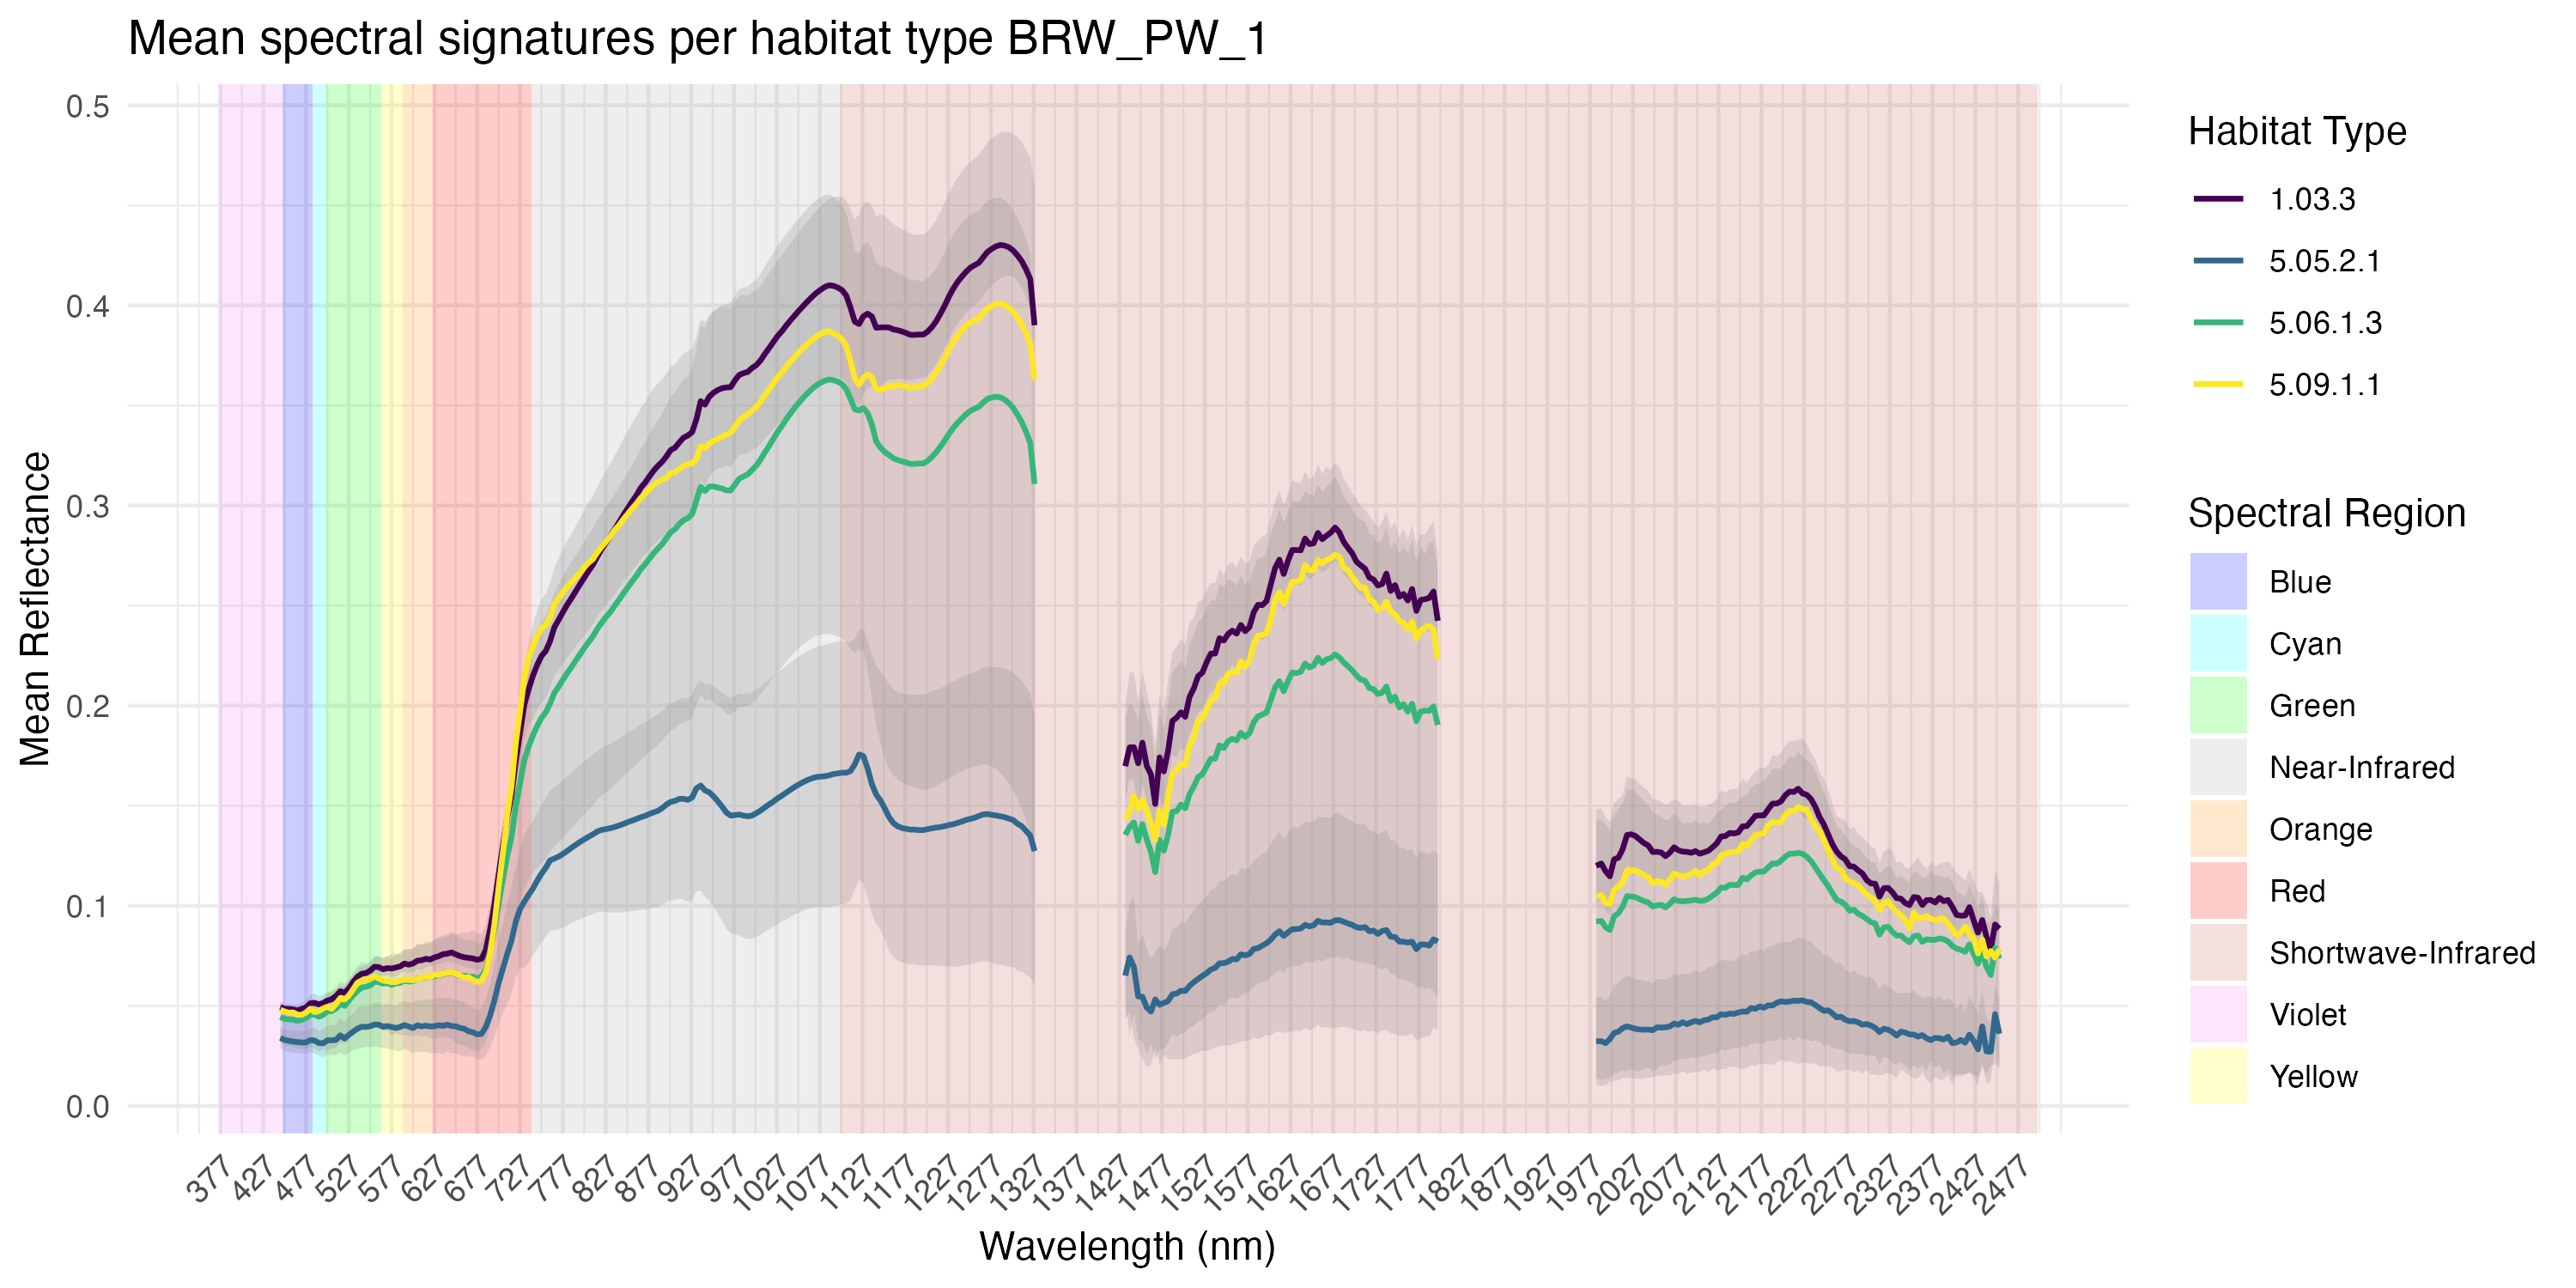
\includegraphics[width=\textwidth]{Figures/spectral_signatures/BRW_PW_1_mean_signature_plot_habitat.png}
    \caption{}
    \label{fig:mss_ht_brwpw1}
  \end{subfigure}

  \caption{Spectral signature plot \ref{fig:ss_ht_brwpw1} and mean spectral signature plot \ref{fig:mss_ht_brwpw1} grouped by habitat type for test site BRW\_PW\_1}
  \label{fig:group_ss_ht_brwpw1}
\end{figure}

\begin{figure}[H]
  \centering

  \begin{subfigure}[b]{0.49\textwidth}
    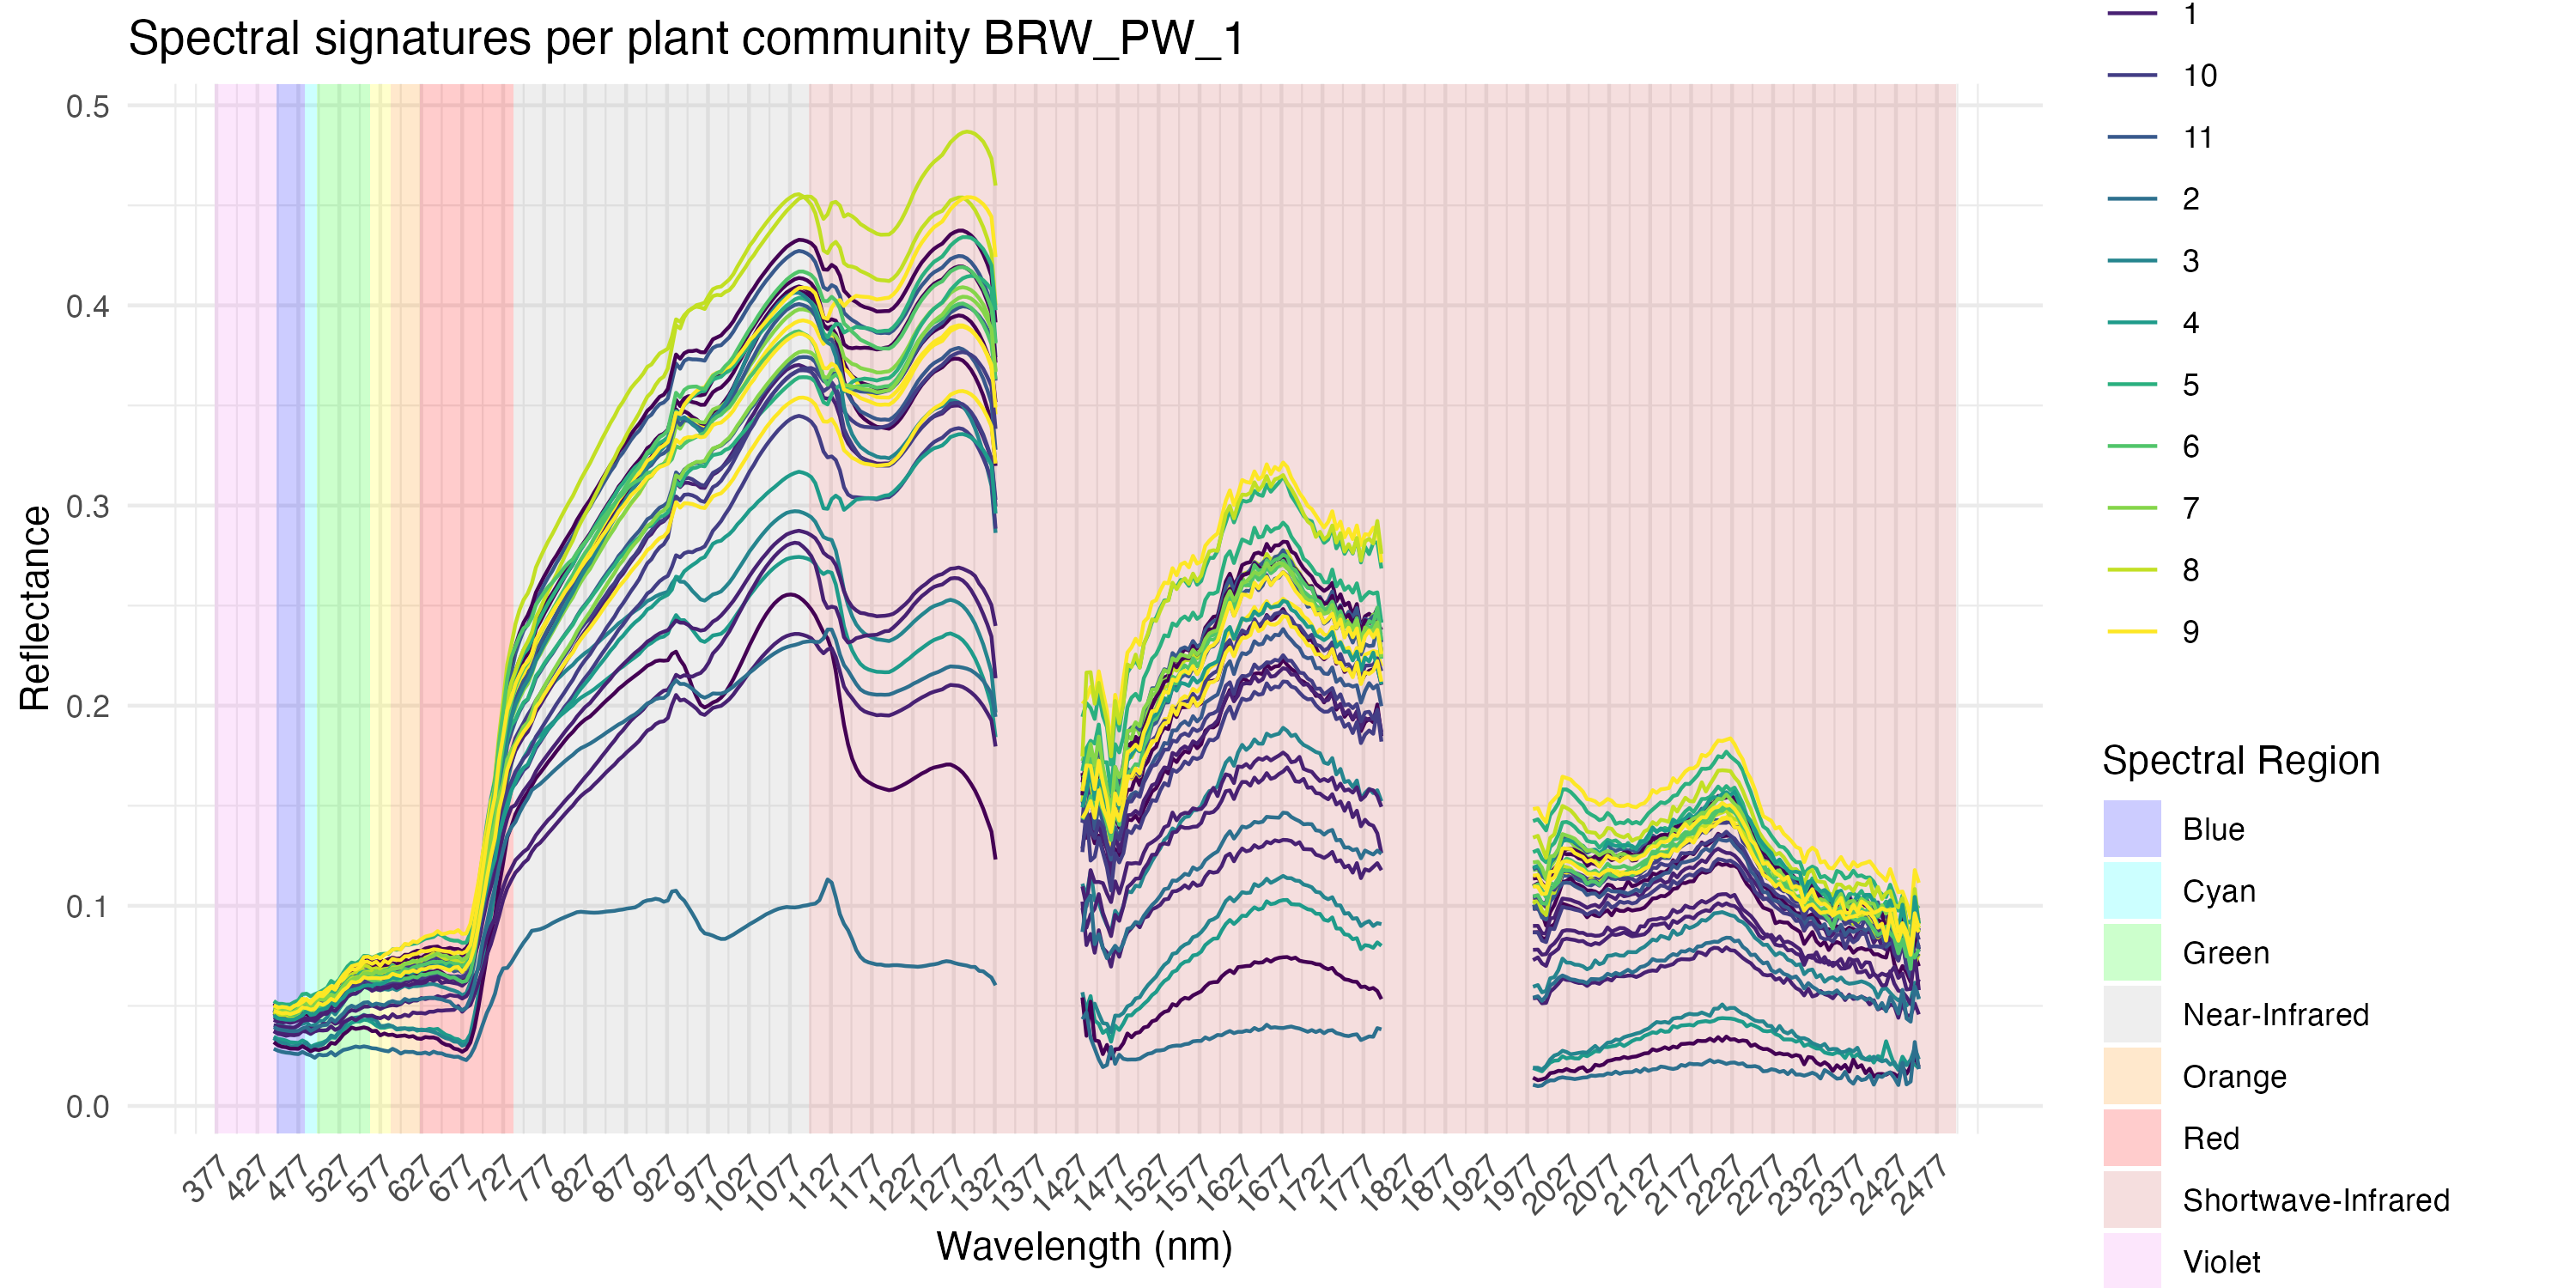
\includegraphics[width=\textwidth]{Figures/spectral_signatures/BRW_PW_1_signature_plot_plant_community.png}
    \caption{}
    \label{fig:ss_pc_brwpw1}
  \end{subfigure}
  \hfill
  \begin{subfigure}[b]{0.49\textwidth}
    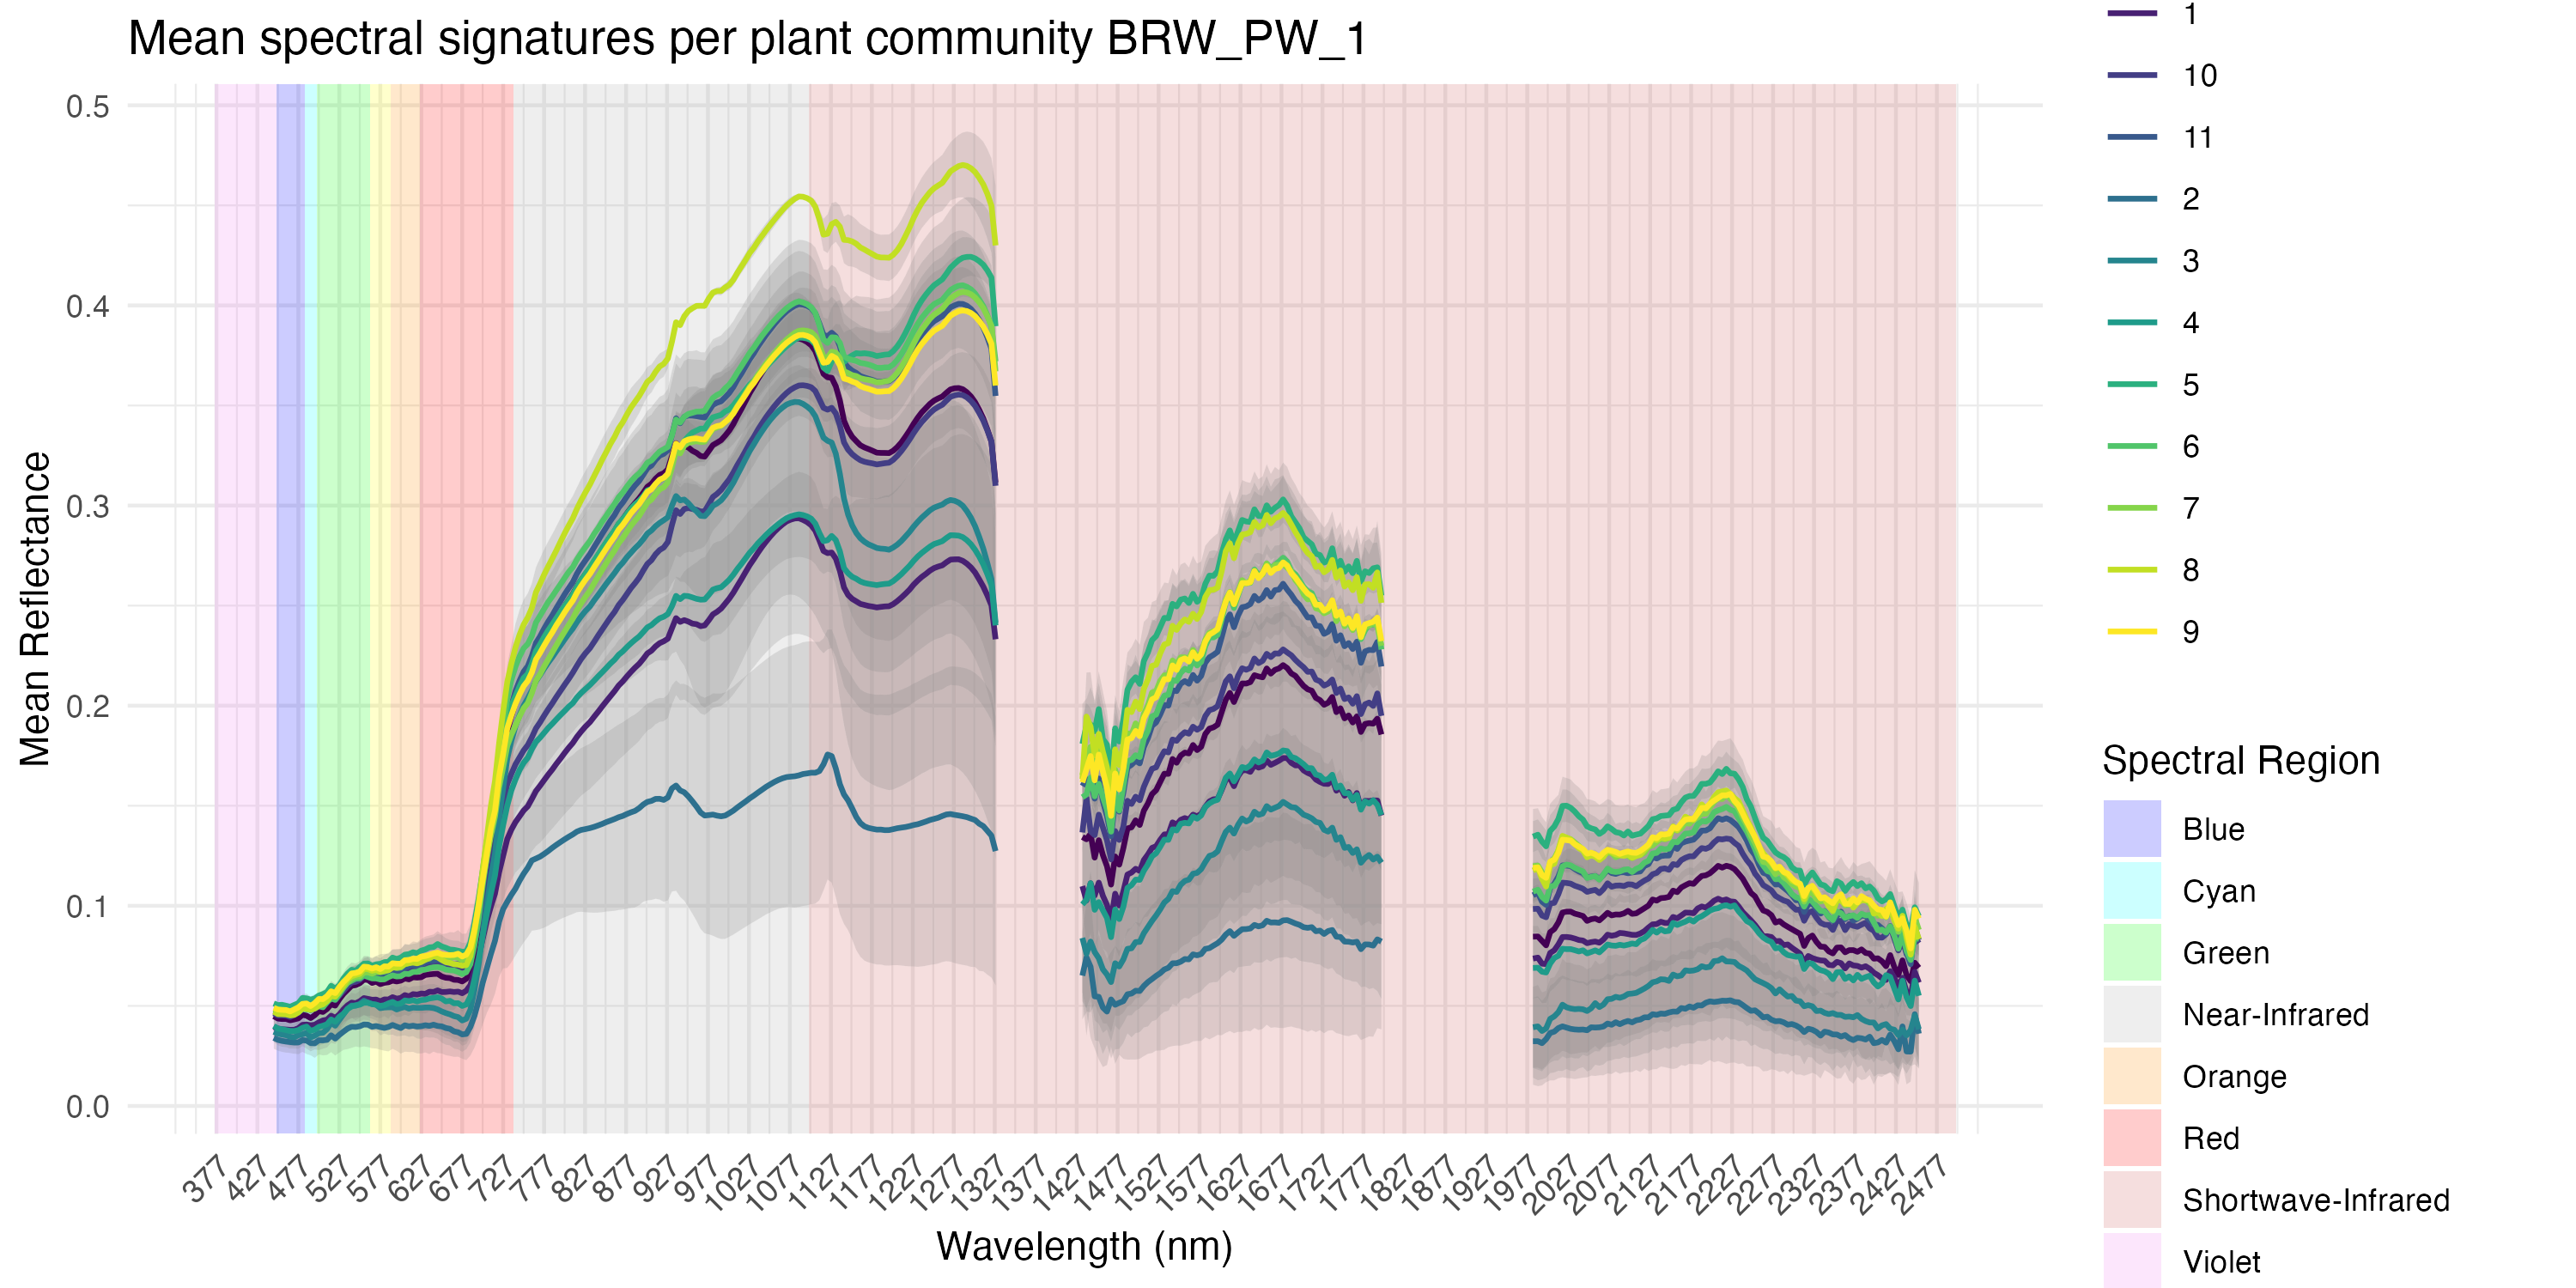
\includegraphics[width=\textwidth]{Figures/spectral_signatures/BRW_PW_1_mean_signature_plot_plant_community.png}
    \caption{}
    \label{fig:mss_pc_brwpw1}
  \end{subfigure}

  \caption{Spectral signature plot \ref{fig:ss_pc_brwpw1} and mean spectral signature plot \ref{fig:mss_pc_brwpw1} grouped by plant community cluster for test site BRW\_PW\_1}
  \label{fig:group_pc_ht_brwpw1}
\end{figure}

\subsection{BRW\_VS\_1}

\begin{figure}[H]
  \centering

  \begin{subfigure}[b]{0.49\textwidth}
    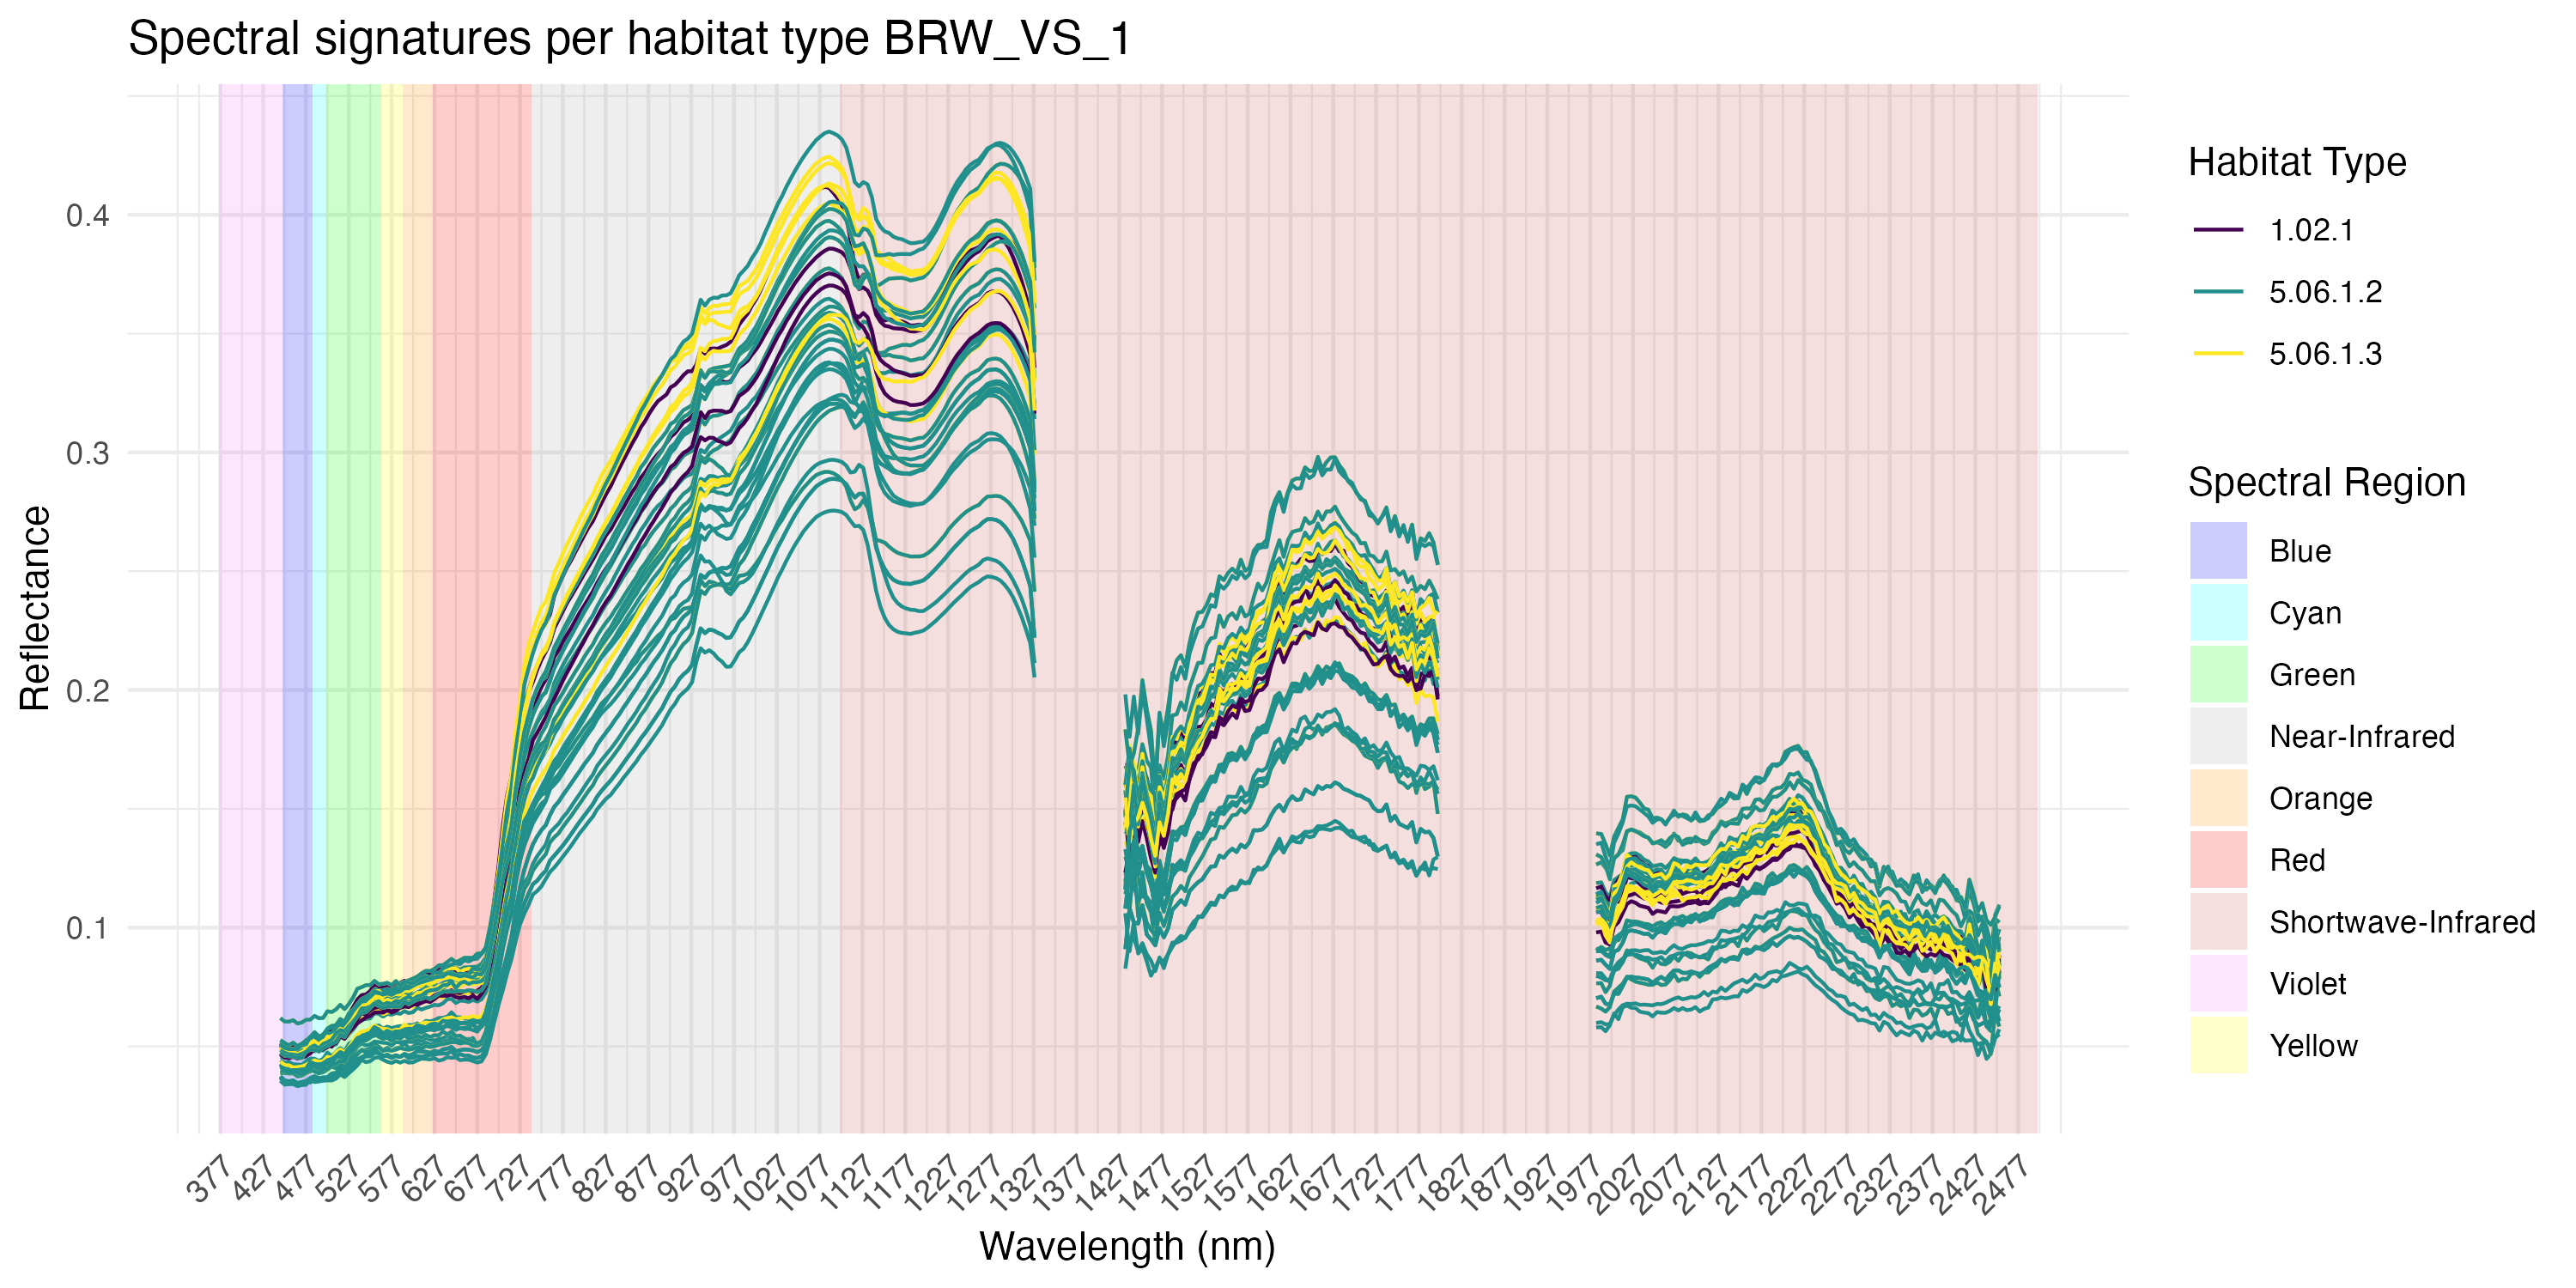
\includegraphics[width=\textwidth]{Figures/spectral_signatures/BRW_VS_1_signature_plot_habitat.png}
    \caption{}
    \label{fig:ss_ht_brwvs1}
  \end{subfigure}
  \hfill
  \begin{subfigure}[b]{0.49\textwidth}
    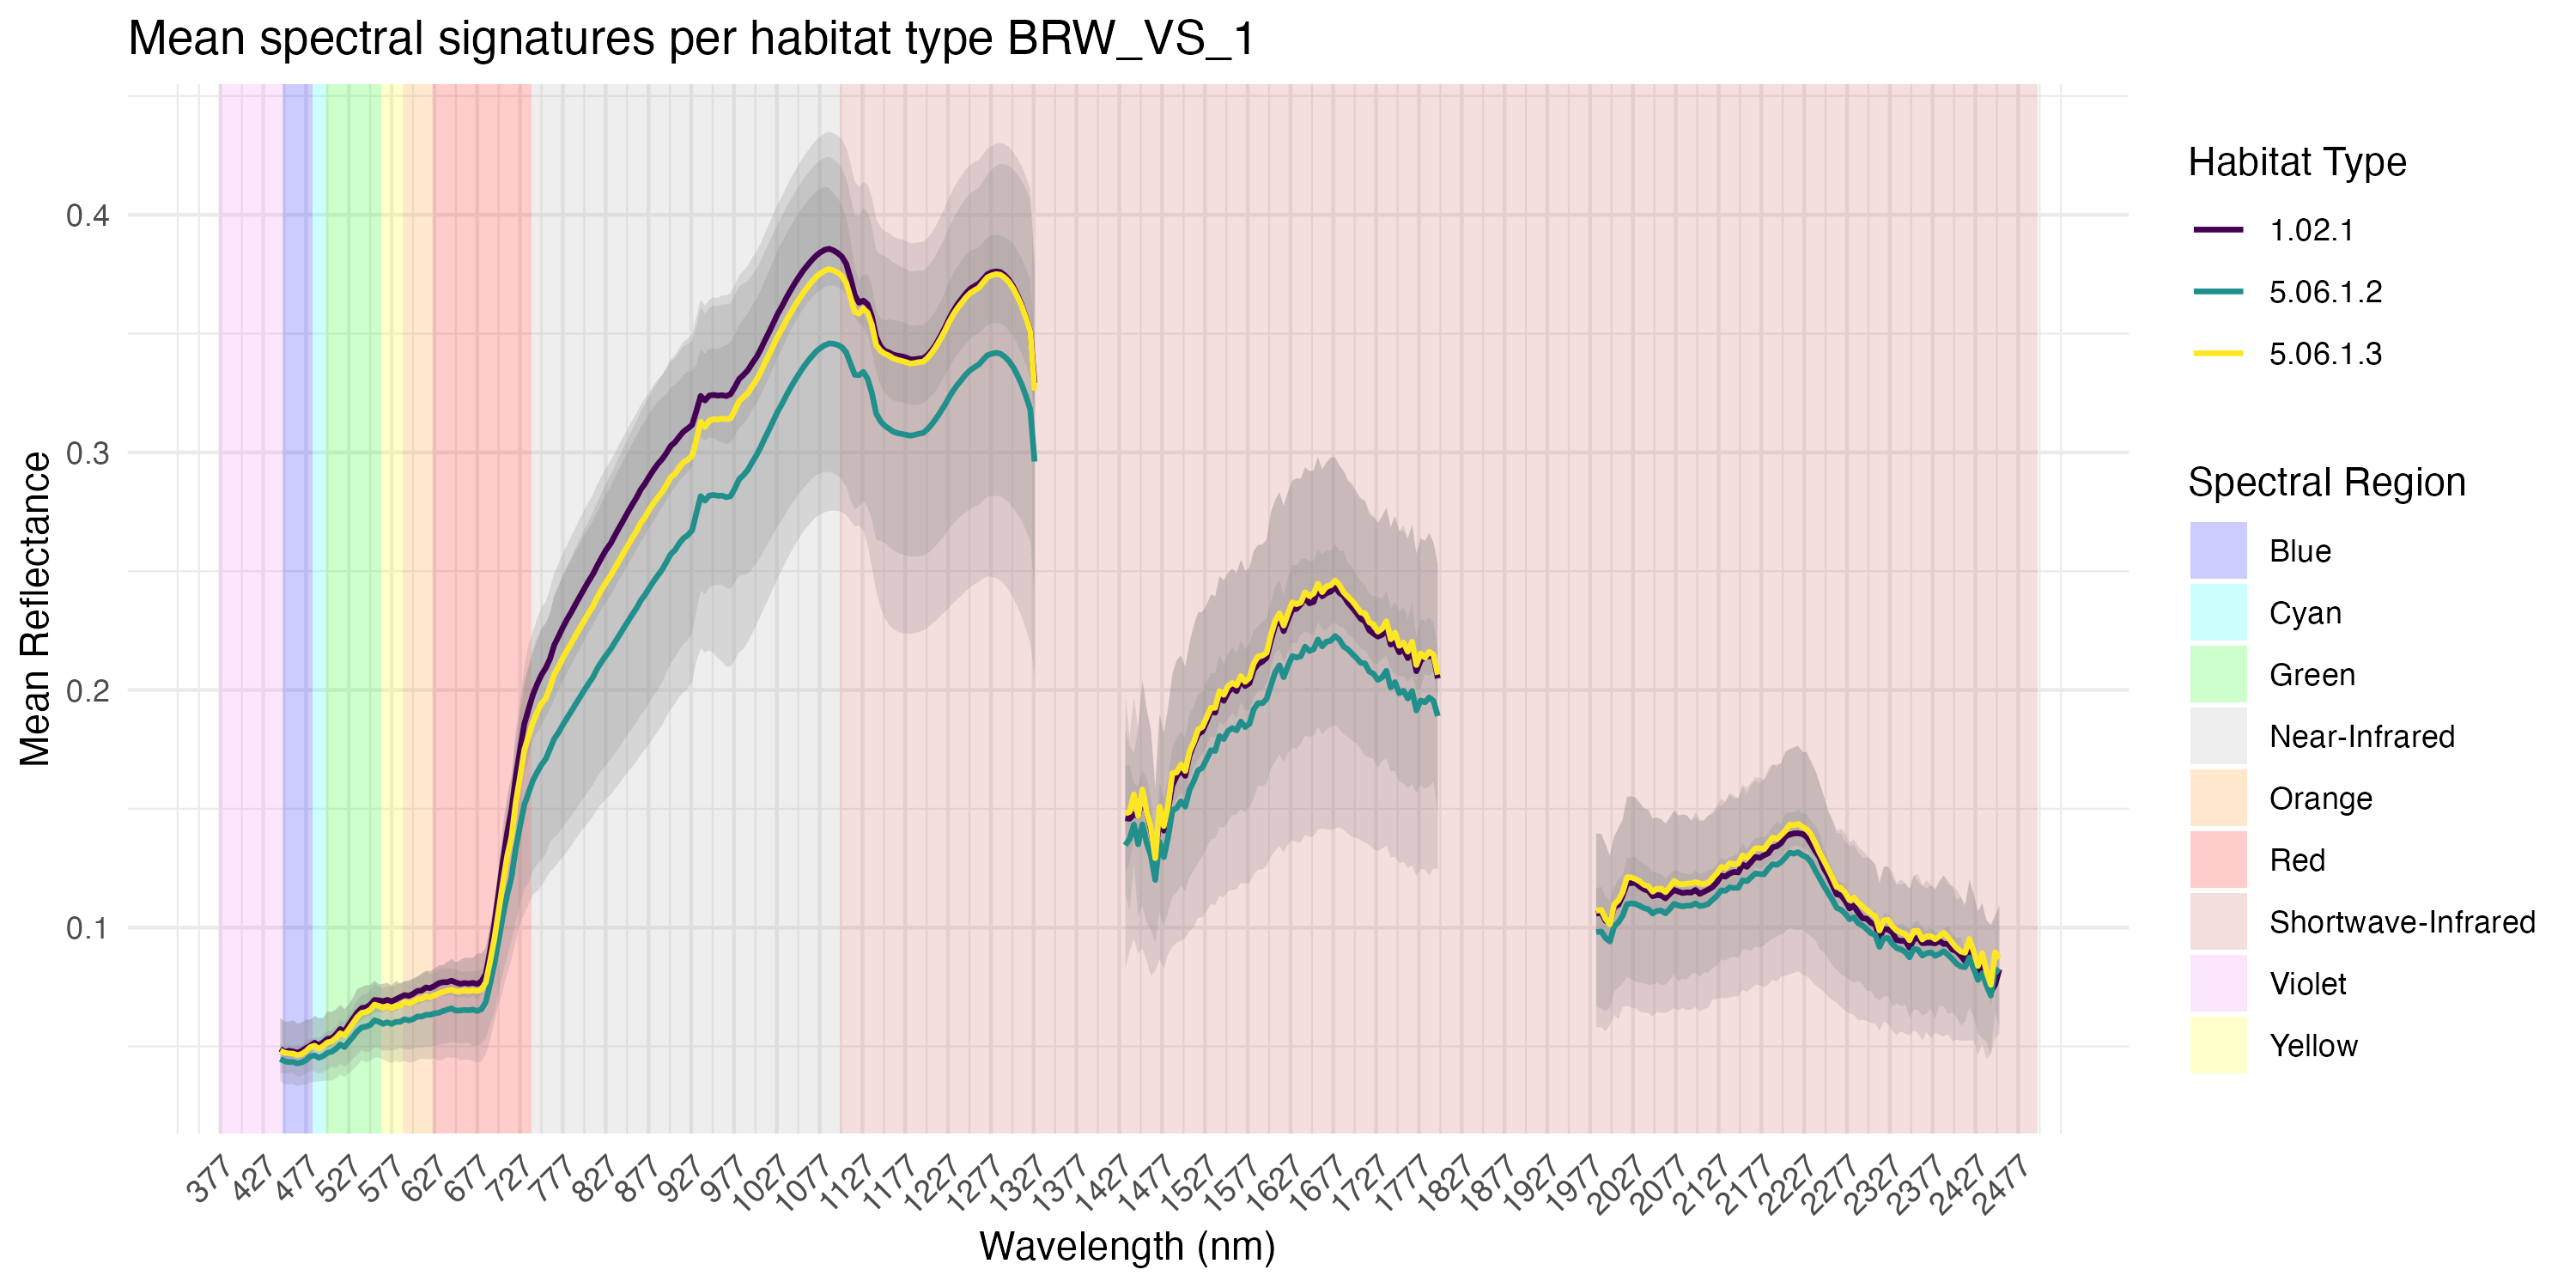
\includegraphics[width=\textwidth]{Figures/spectral_signatures/BRW_VS_1_mean_signature_plot_habitat.png}
    \caption{}
    \label{fig:mss_ht_brwvs1}
  \end{subfigure}

  \caption{Spectral signature plot \ref{fig:ss_ht_brwvs1} and mean spectral signature plot \ref{fig:mss_ht_brwvs1} grouped by habitat type for test site BRW\_VS\_1}
  \label{fig:group_ss_ht_brwvs1}
\end{figure}

\begin{figure}[H]
  \centering

  \begin{subfigure}[b]{0.49\textwidth}
    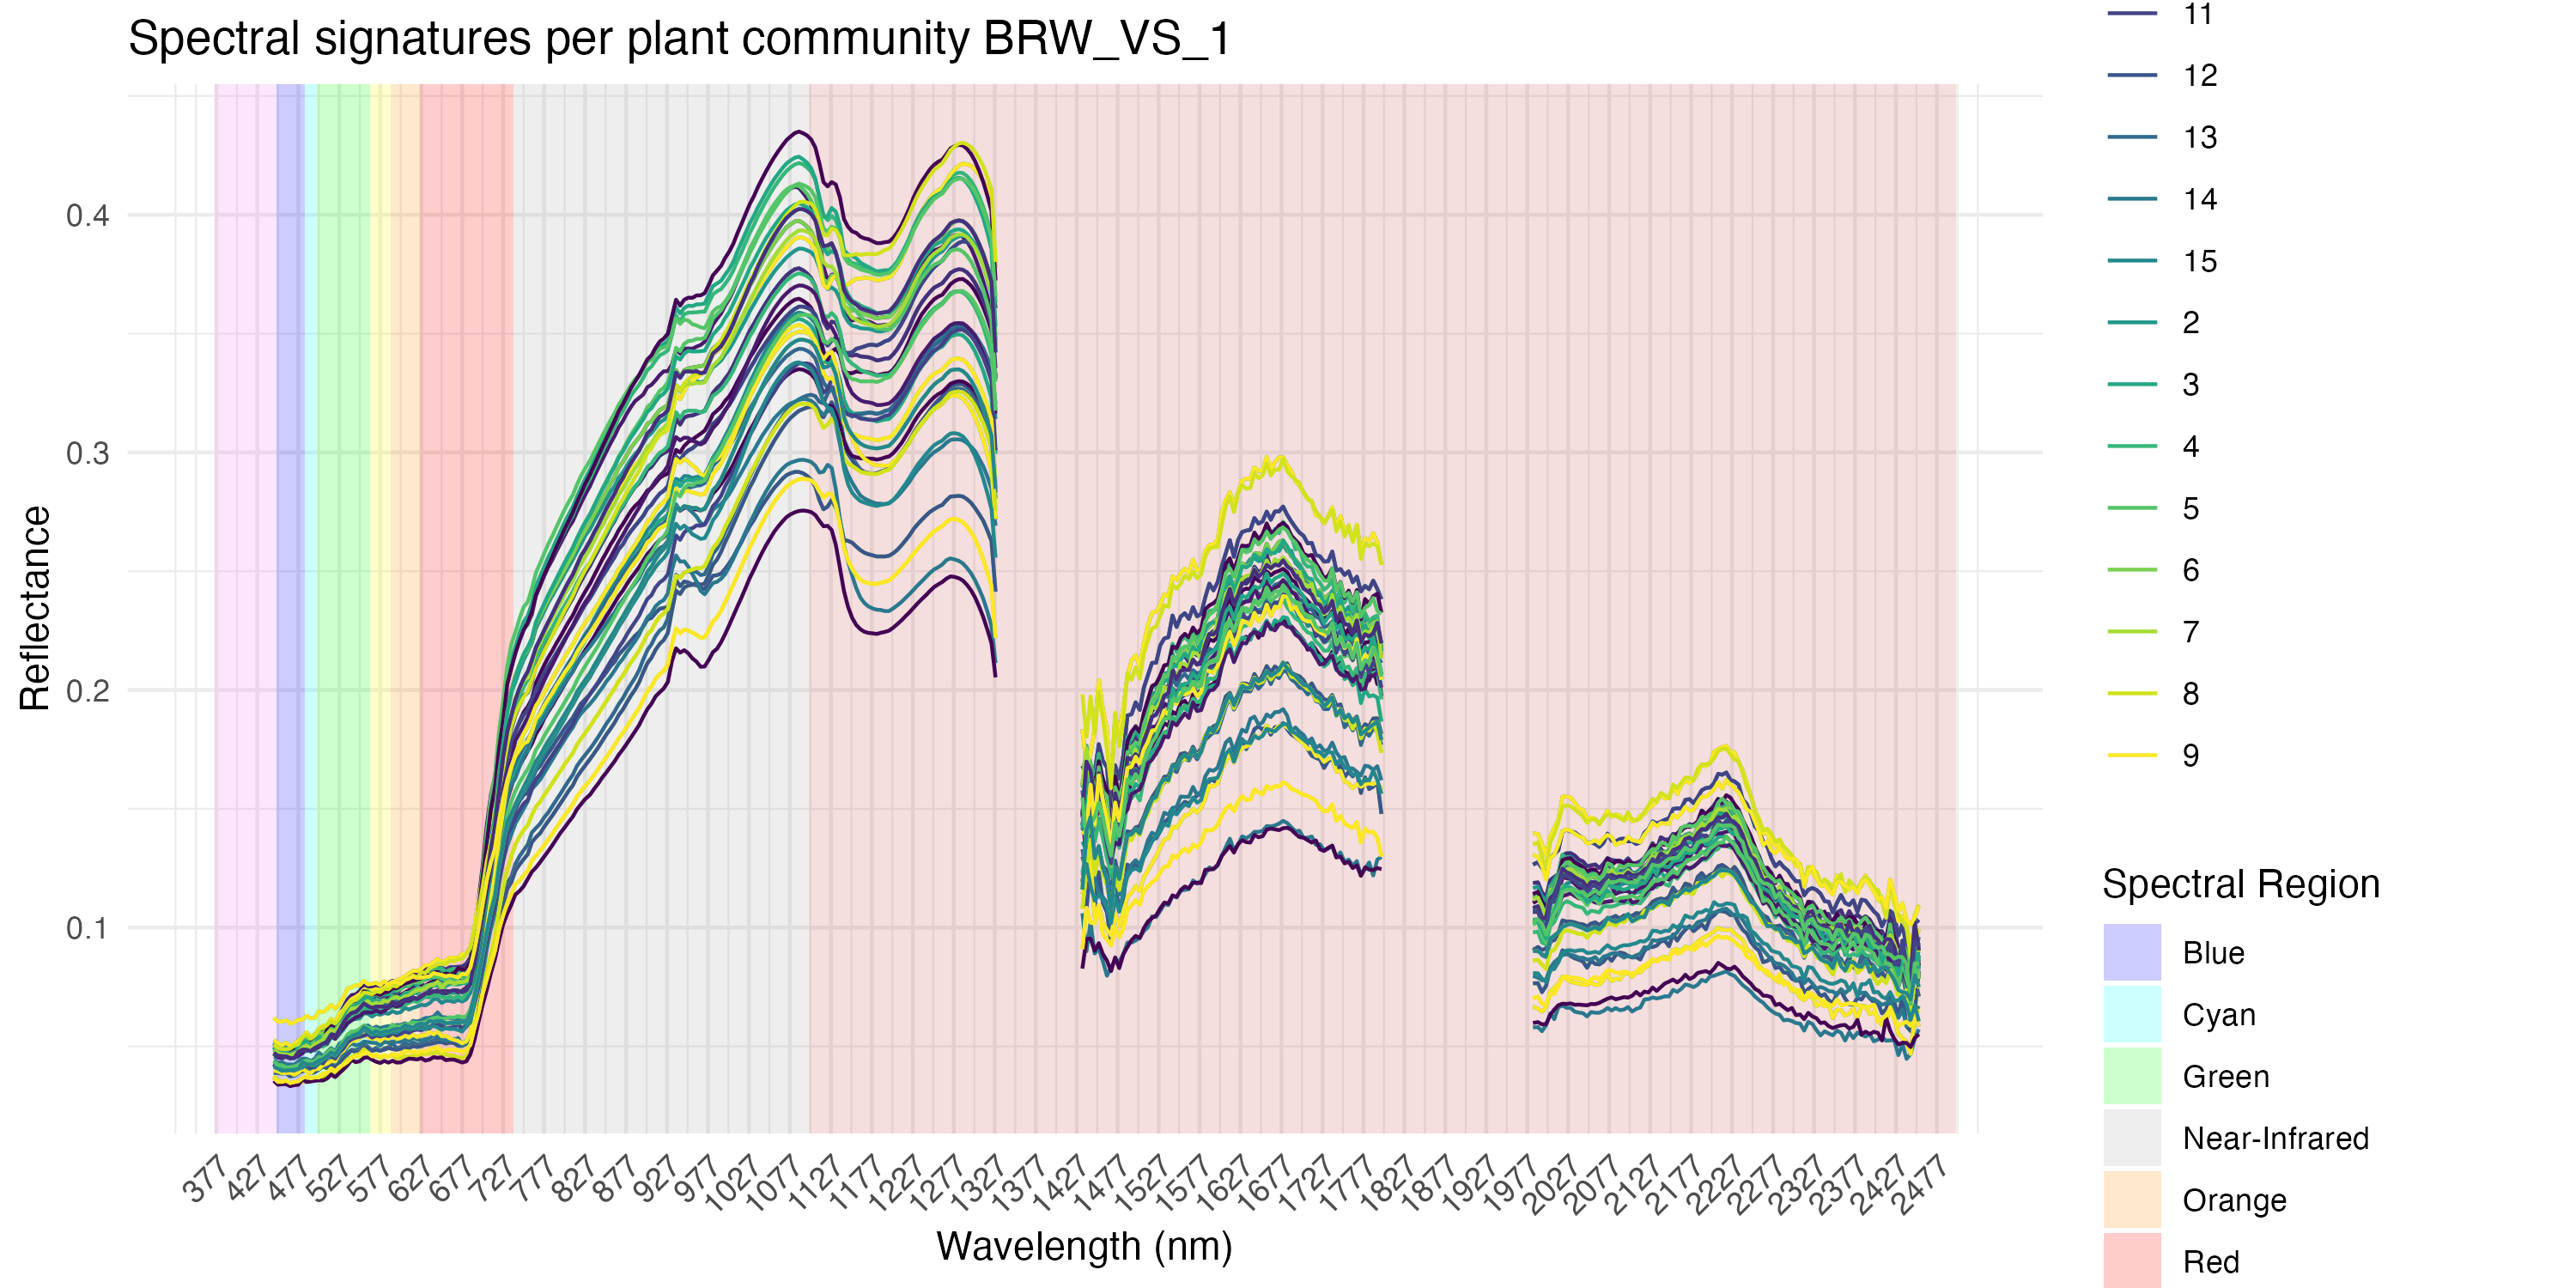
\includegraphics[width=\textwidth]{Figures/spectral_signatures/BRW_VS_1_signature_plot_plant_community.png}
    \caption{}
    \label{fig:ss_pc_brwvs1}
  \end{subfigure}
  \hfill
  \begin{subfigure}[b]{0.49\textwidth}
    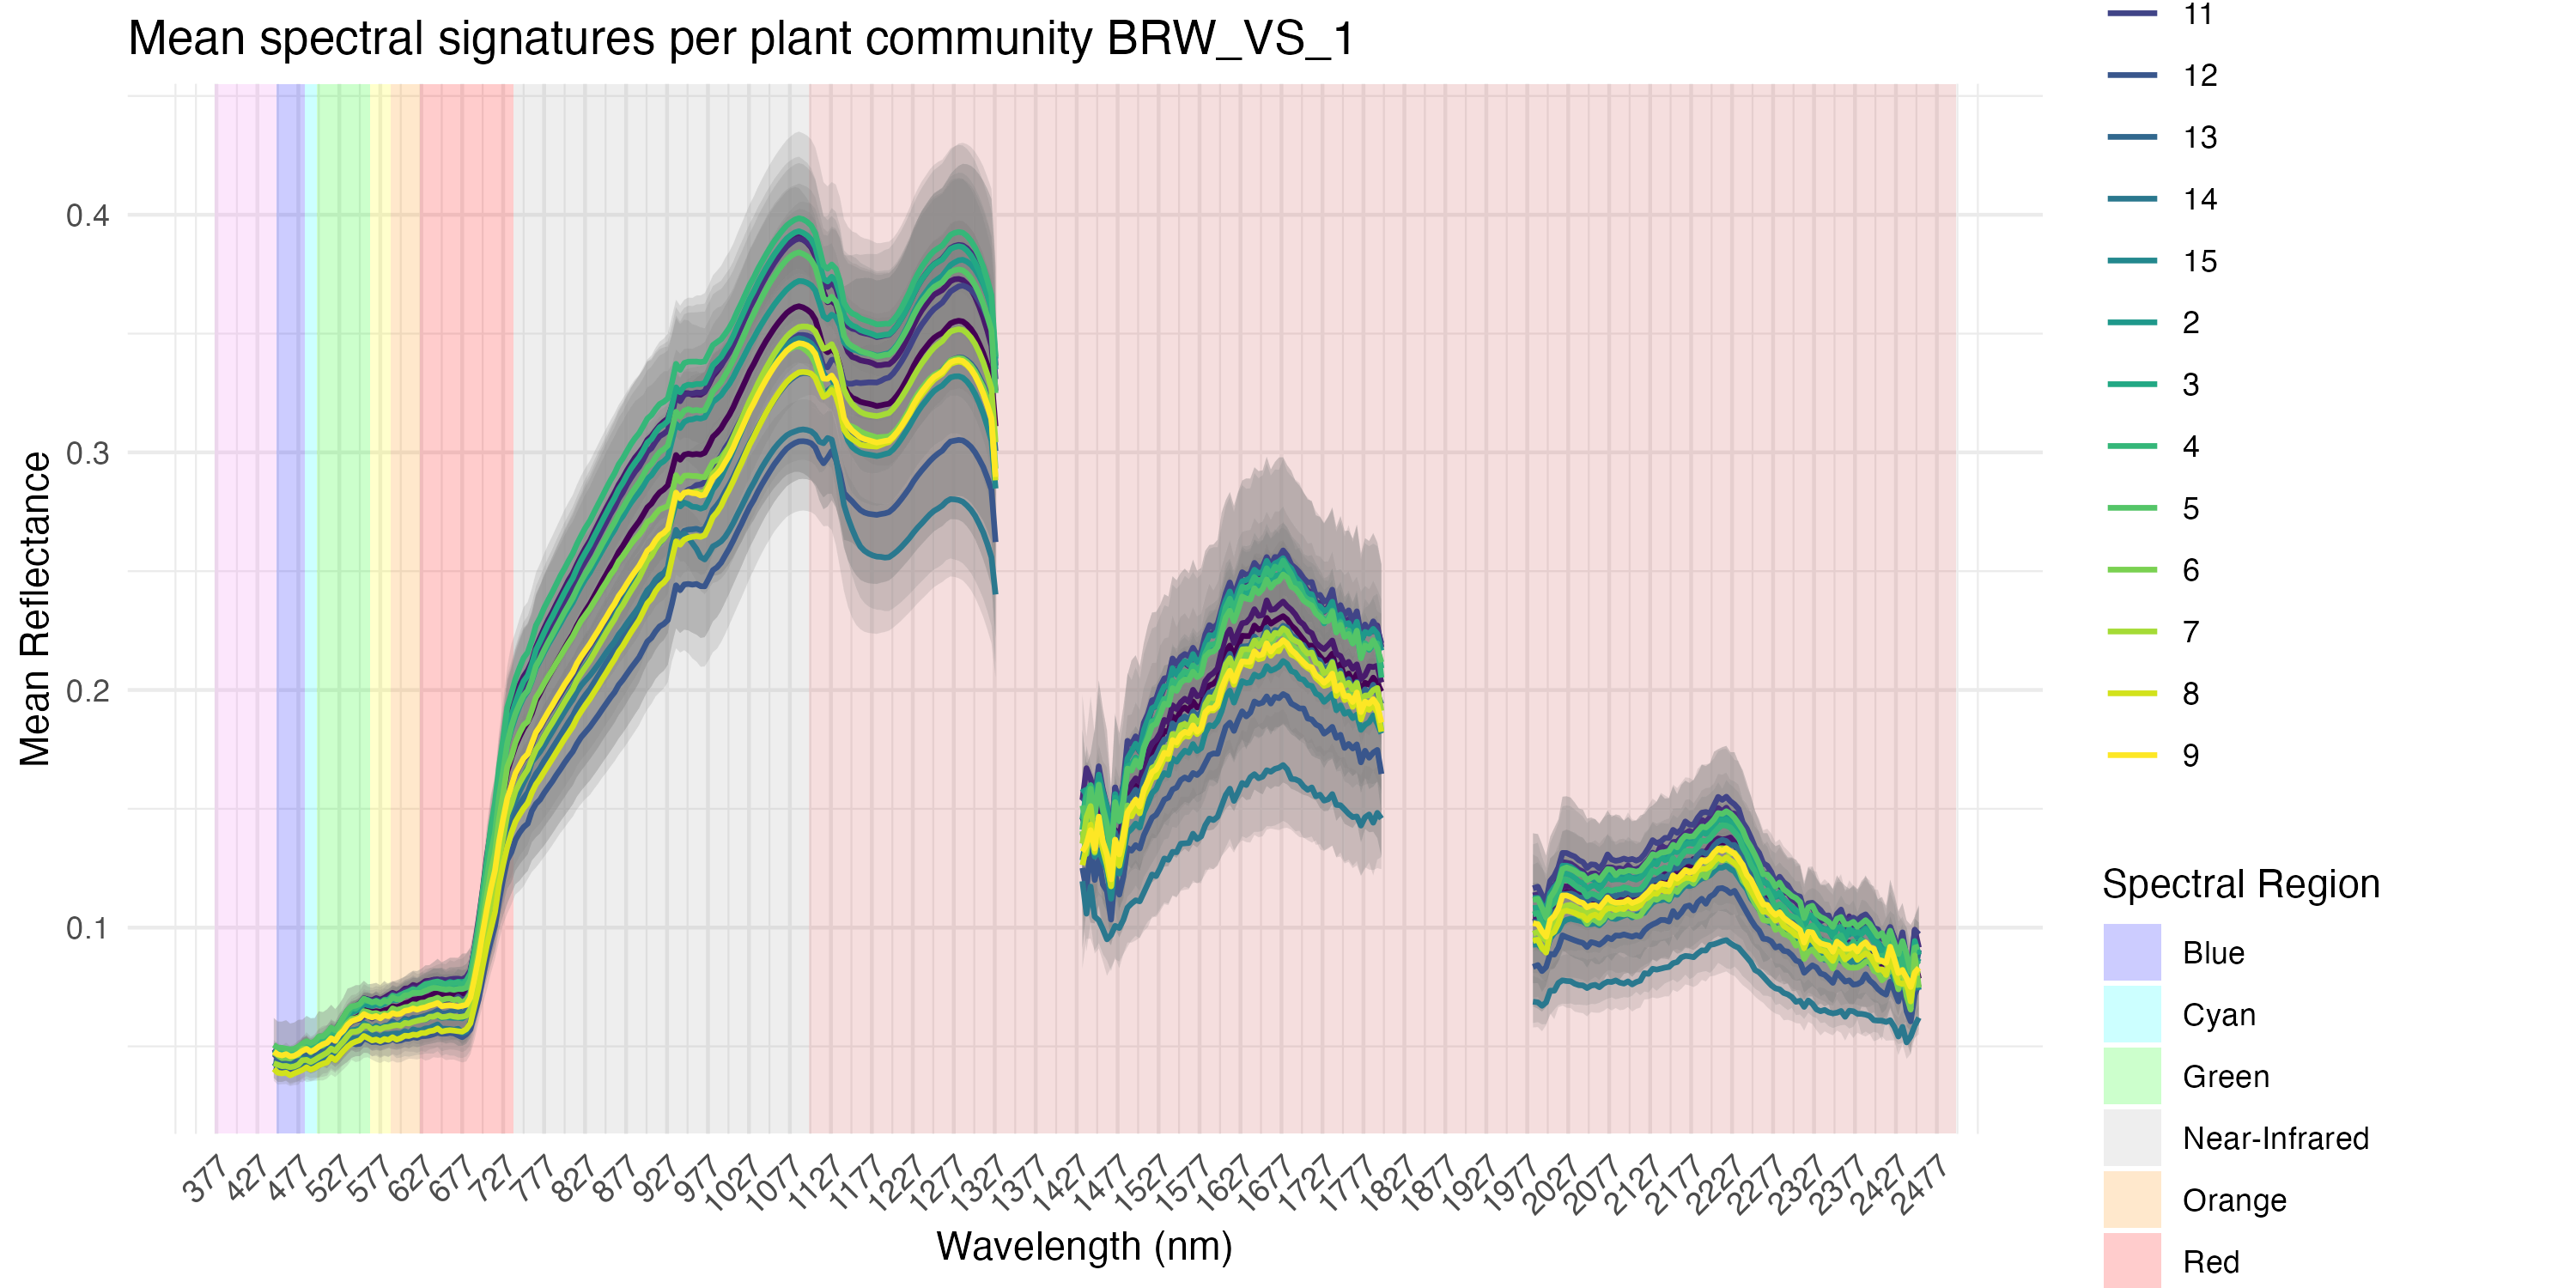
\includegraphics[width=\textwidth]{Figures/spectral_signatures/BRW_VS_1_mean_signature_plot_plant_community.png}
    \caption{}
    \label{fig:mss_pc_brwvs1}
  \end{subfigure}

  \caption{Spectral signature plot \ref{fig:ss_pc_brwvs1} and mean spectral signature plot \ref{fig:mss_pc_brwvs1} grouped by plant community cluster for test site BRW\_VS\_1}
  \label{fig:group_pc_ht_brwvs1}
\end{figure}

\subsection{FLXTWRZONA\_SD\_1}

\begin{figure}[H]
  \centering

  \begin{subfigure}[b]{0.49\textwidth}
    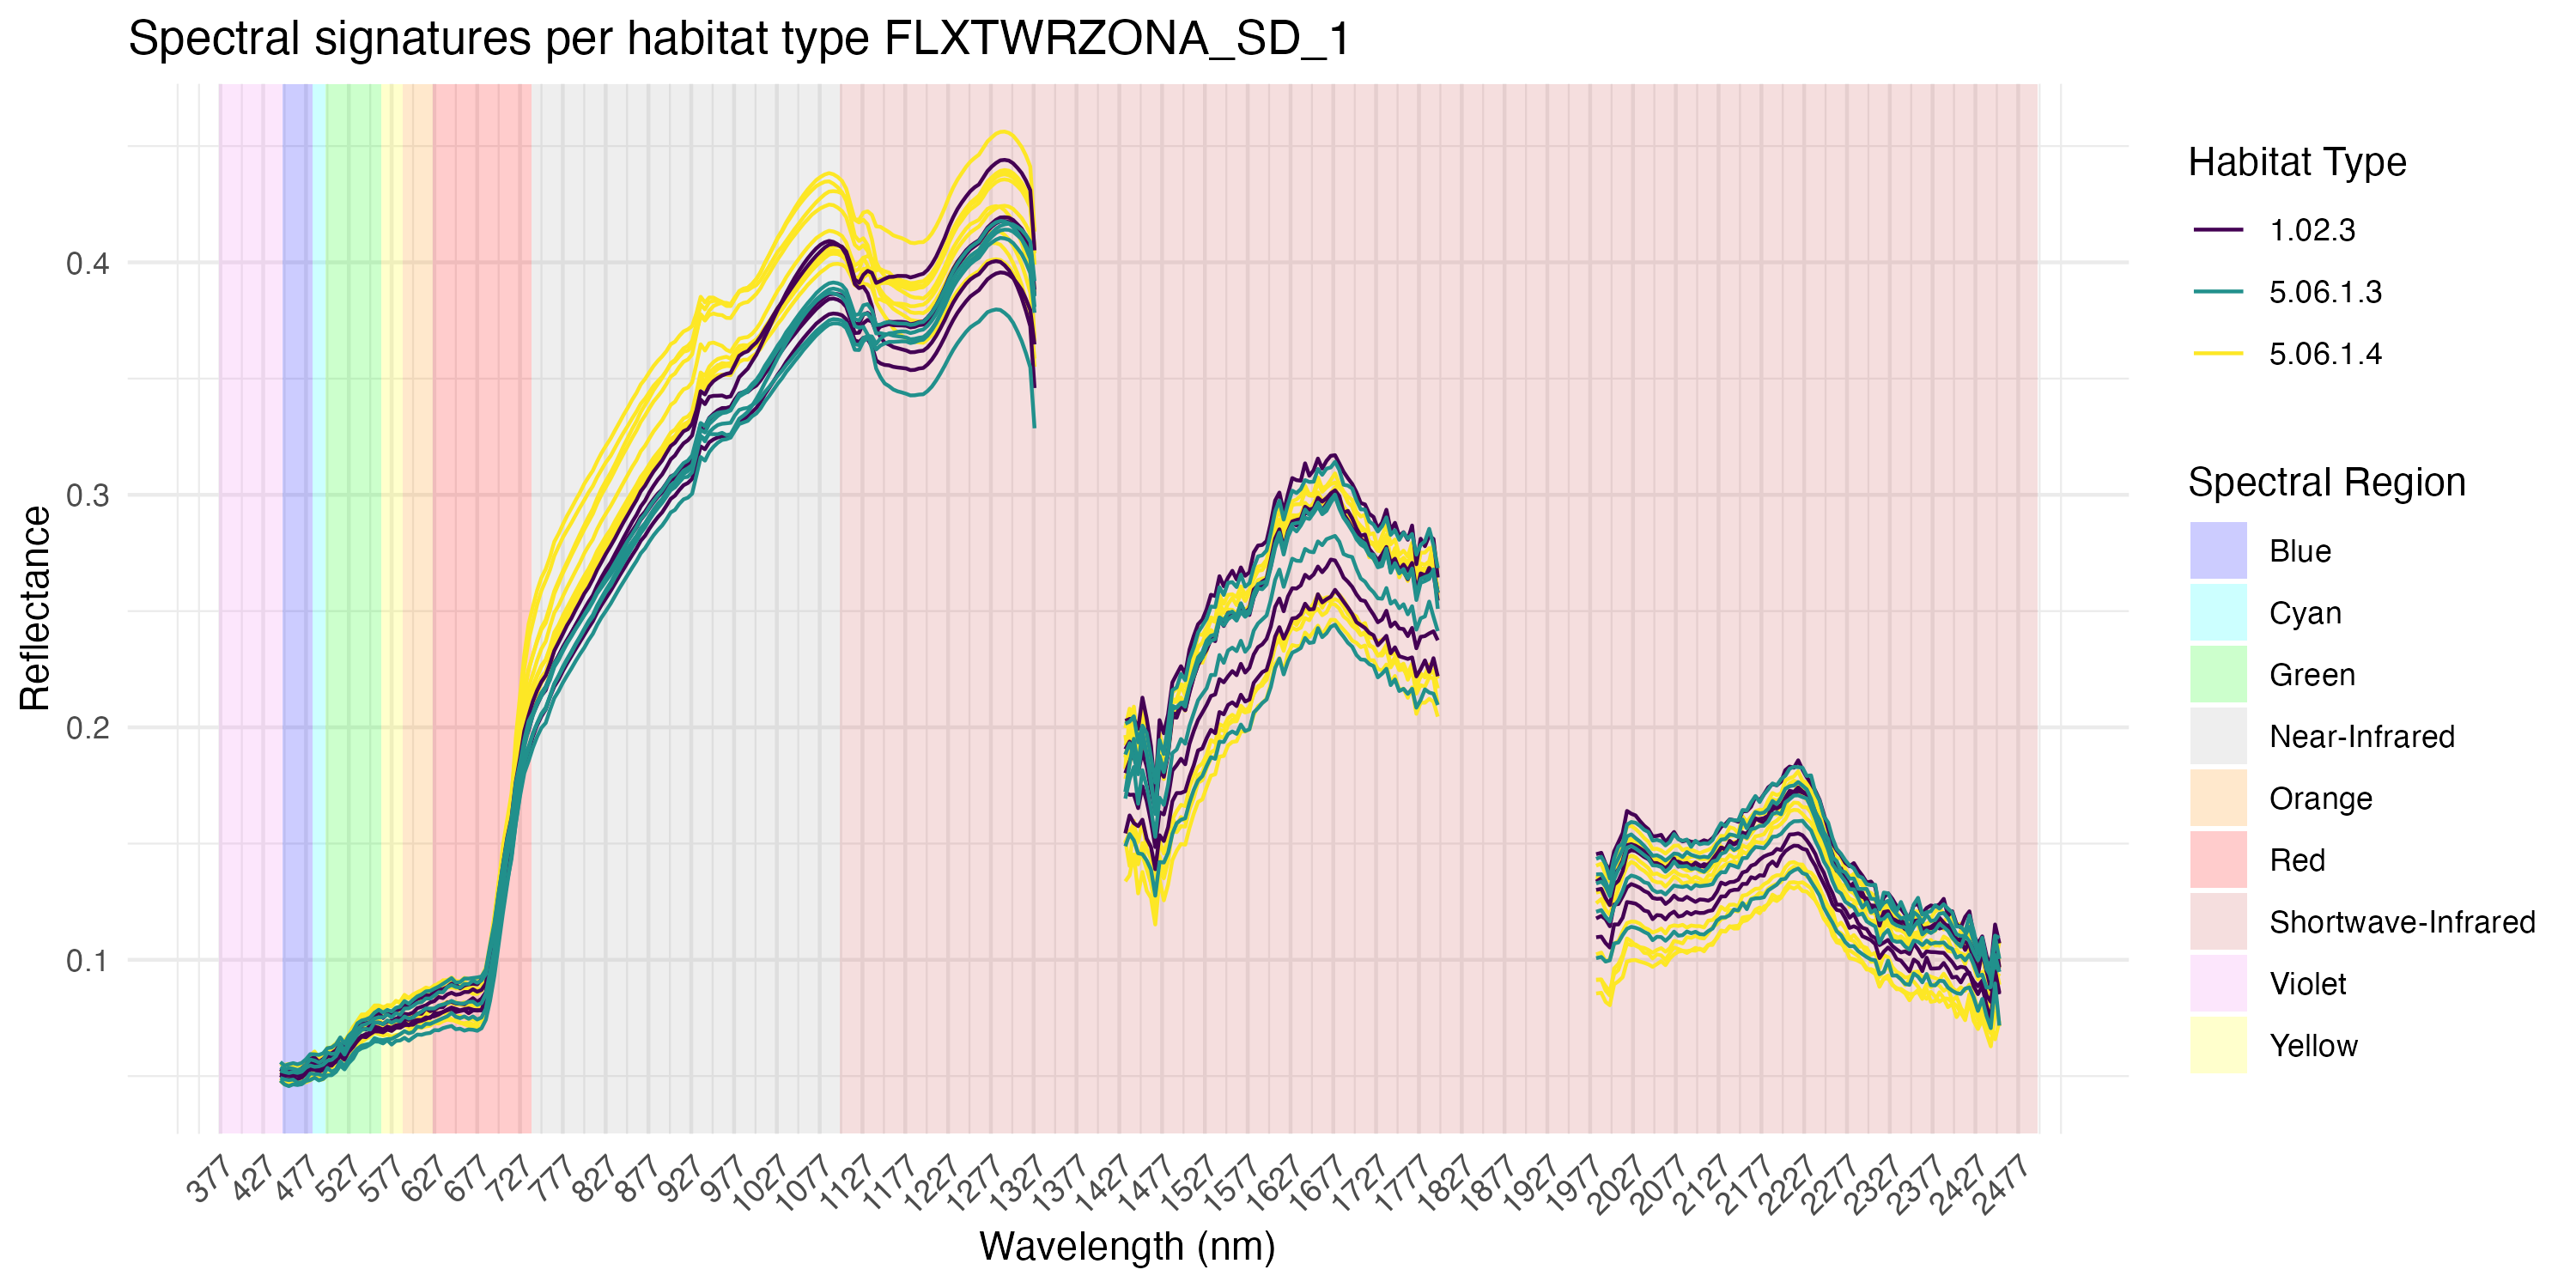
\includegraphics[width=\textwidth]{Figures/spectral_signatures/FLXTWRZONA_SD_1_signature_plot_habitat.png}
    \caption{}
    \label{fig:ss_ht_flxtwrzonasd1}
  \end{subfigure}
  \hfill
  \begin{subfigure}[b]{0.49\textwidth}
    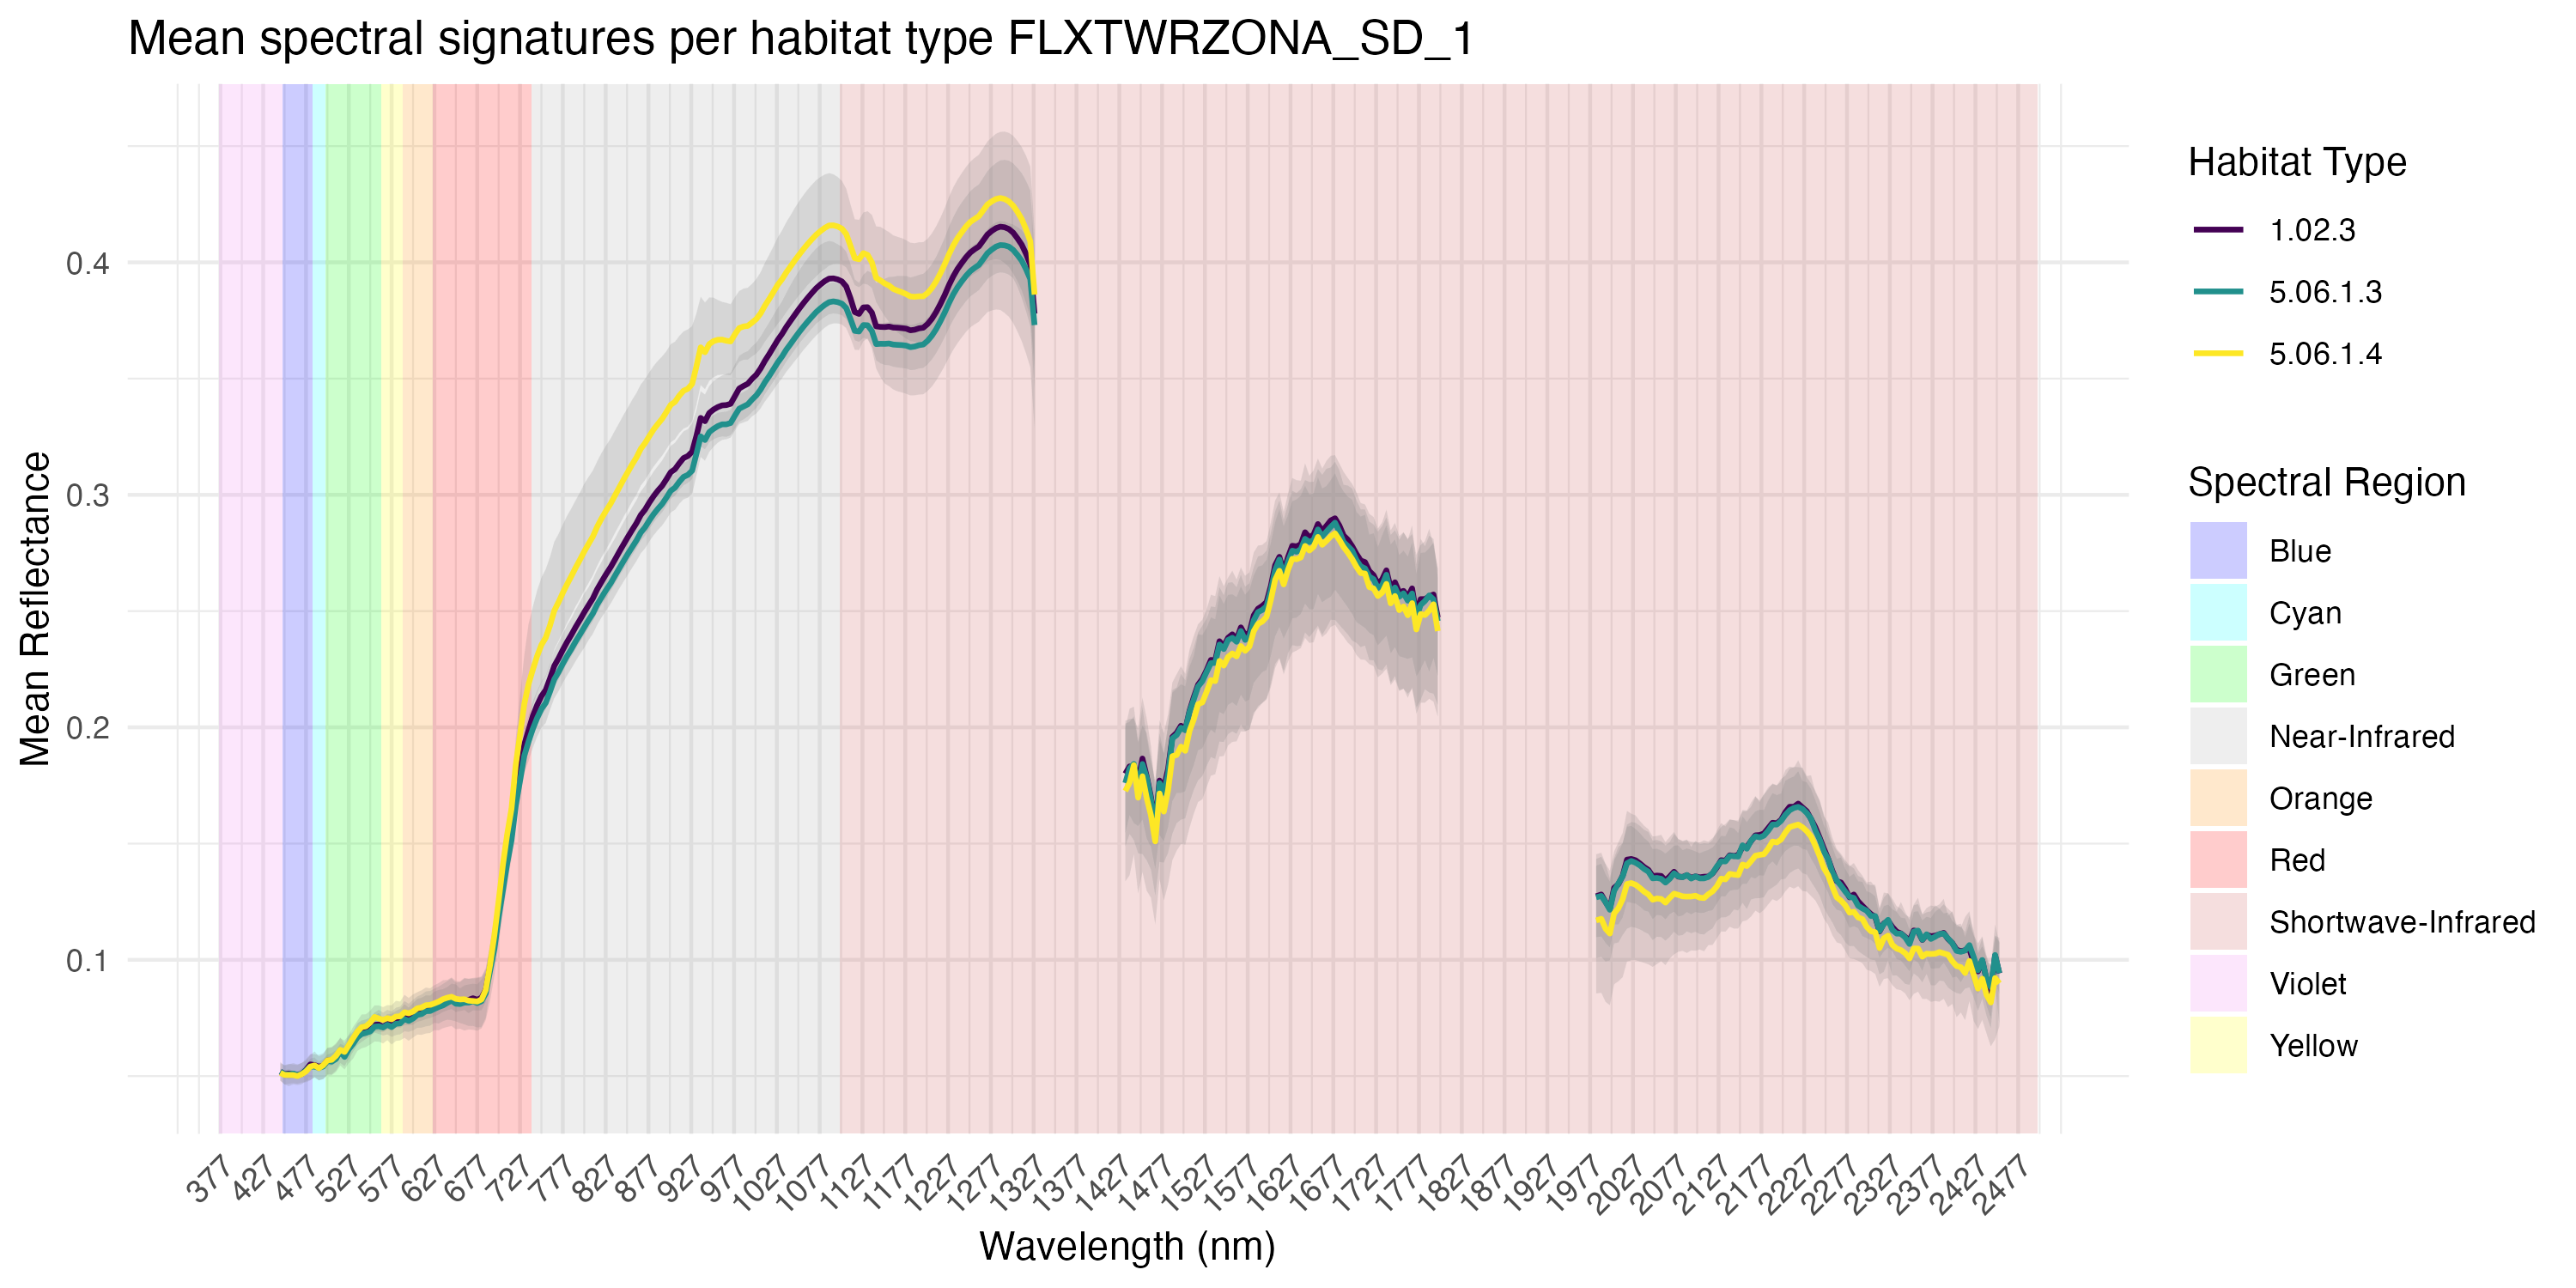
\includegraphics[width=\textwidth]{Figures/spectral_signatures/FLXTWRZONA_SD_1_mean_signature_plot_habitat.png}
    \caption{}
    \label{fig:mss_ht_flxtwrzonasd1}
  \end{subfigure}

  \caption{Spectral signature plot \ref{fig:ss_ht_flxtwrzonasd1} and mean spectral signature plot \ref{fig:mss_ht_flxtwrzonasd1} grouped by habitat type for test site FLXTWRZONA\_SD\_1}
  \label{fig:group_ss_ht_flxtwrzonasd1}
\end{figure}

\begin{figure}[H]
  \centering

  \begin{subfigure}[b]{0.49\textwidth}
    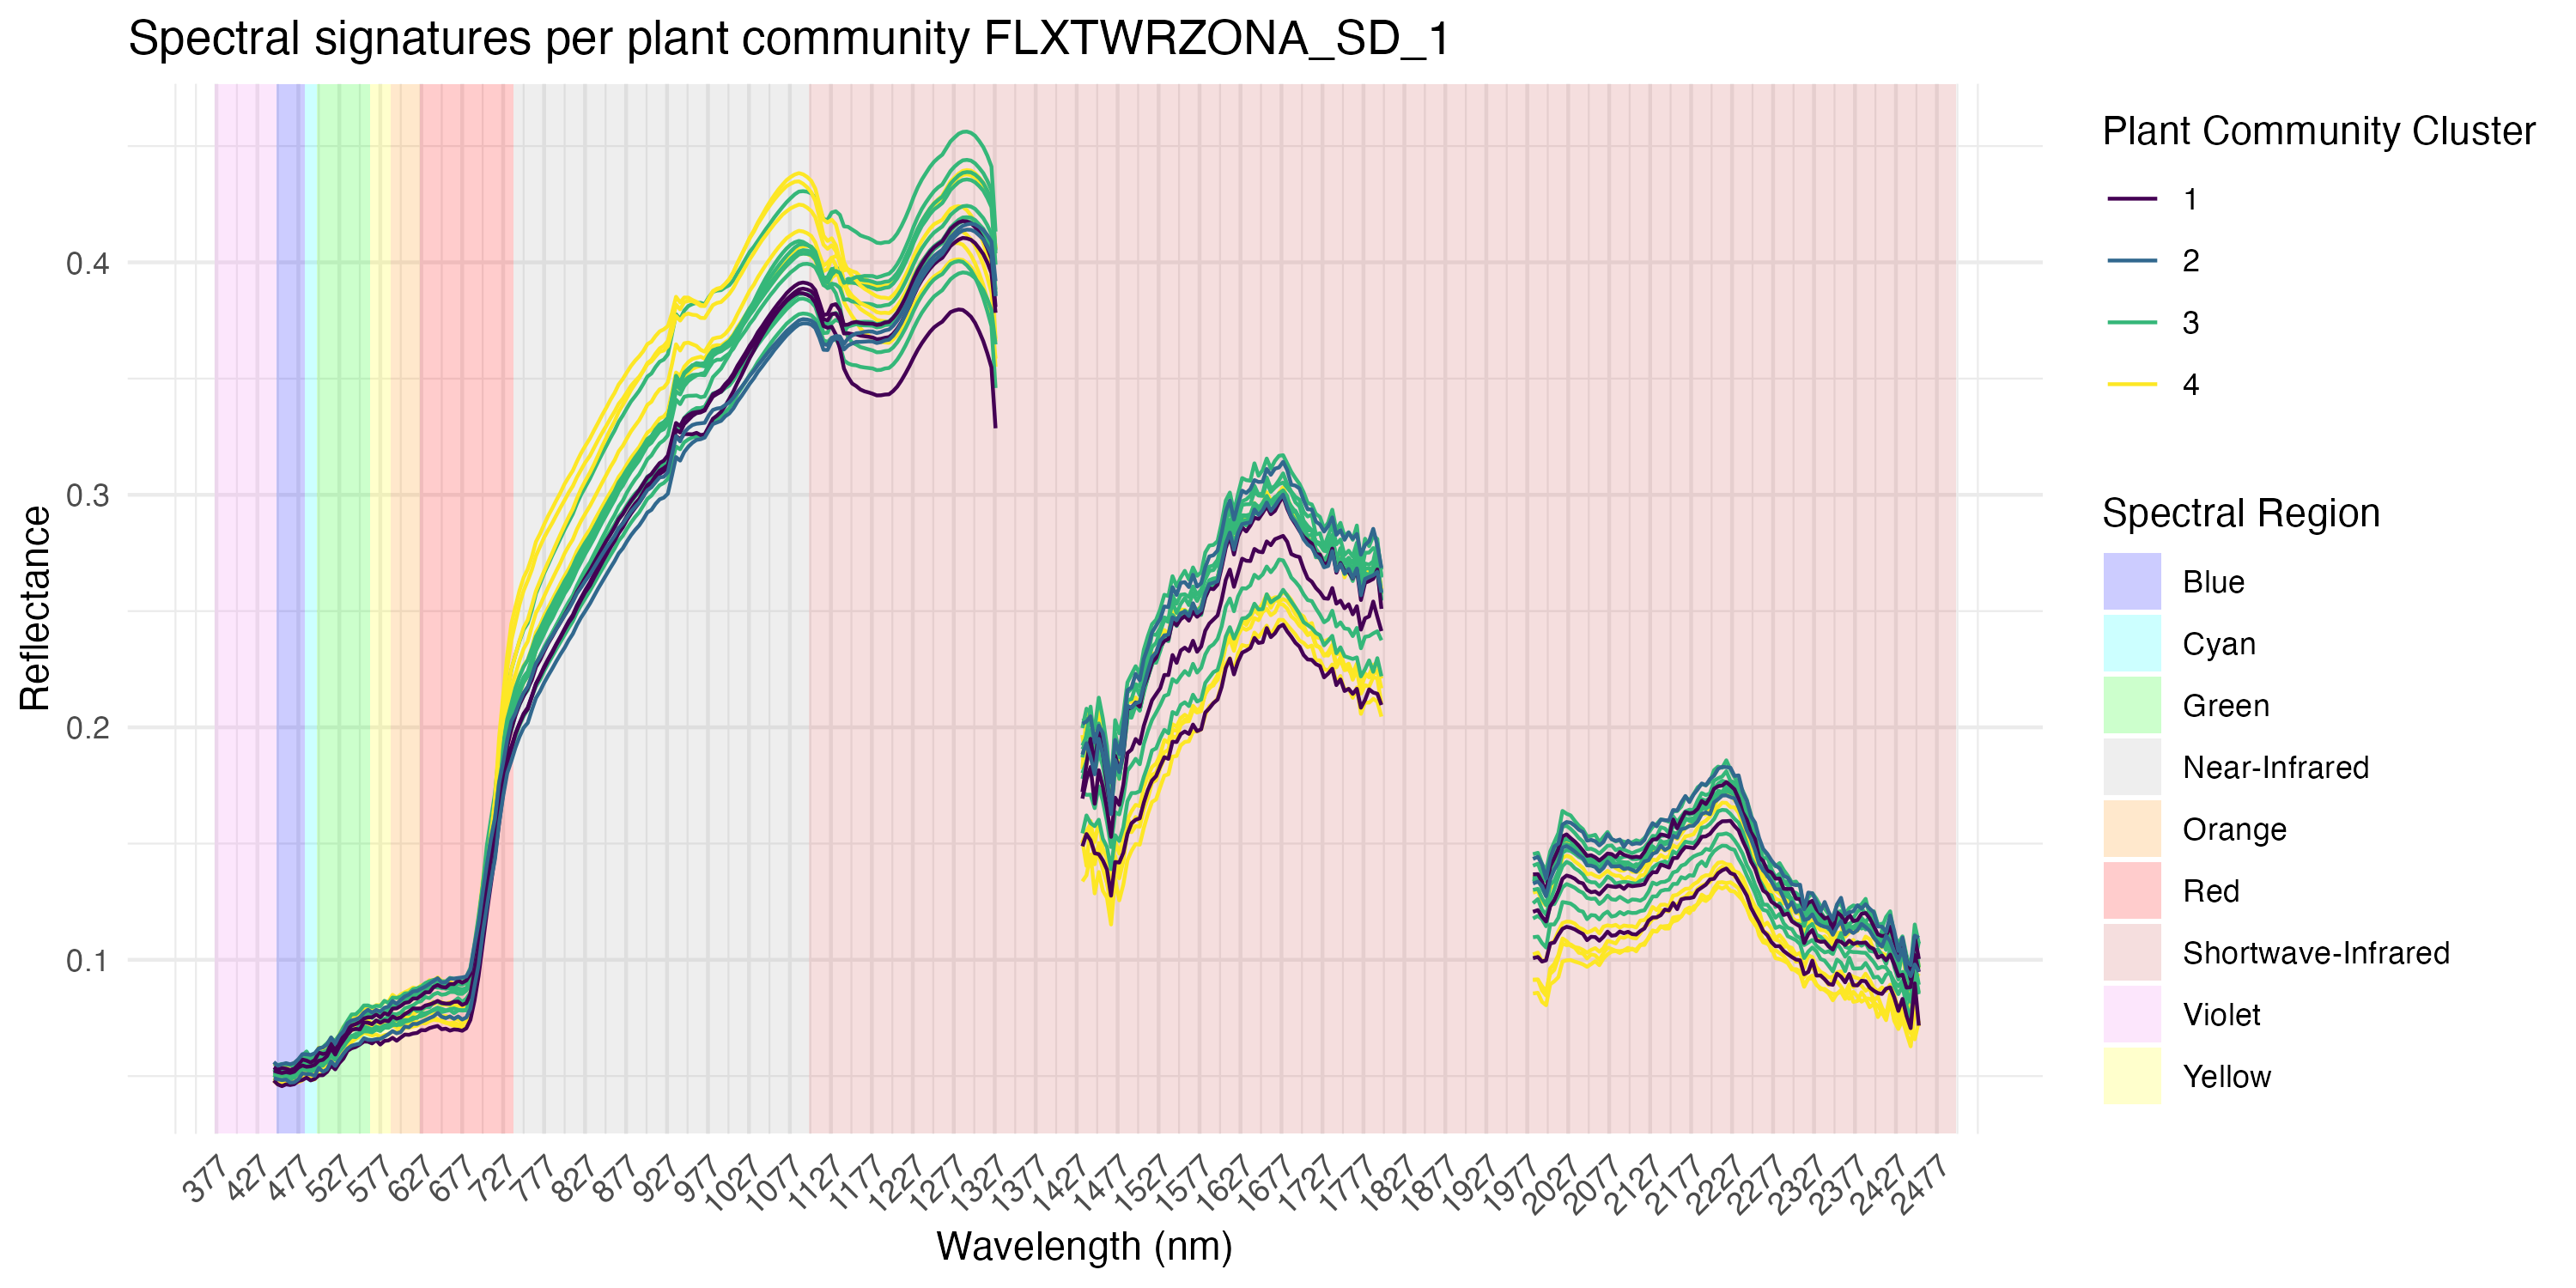
\includegraphics[width=\textwidth]{Figures/spectral_signatures/FLXTWRZONA_SD_1_signature_plot_plant_community.png}
    \caption{}
    \label{fig:ss_pc_flxtwrzonasd1}
  \end{subfigure}
  \hfill
  \begin{subfigure}[b]{0.49\textwidth}
    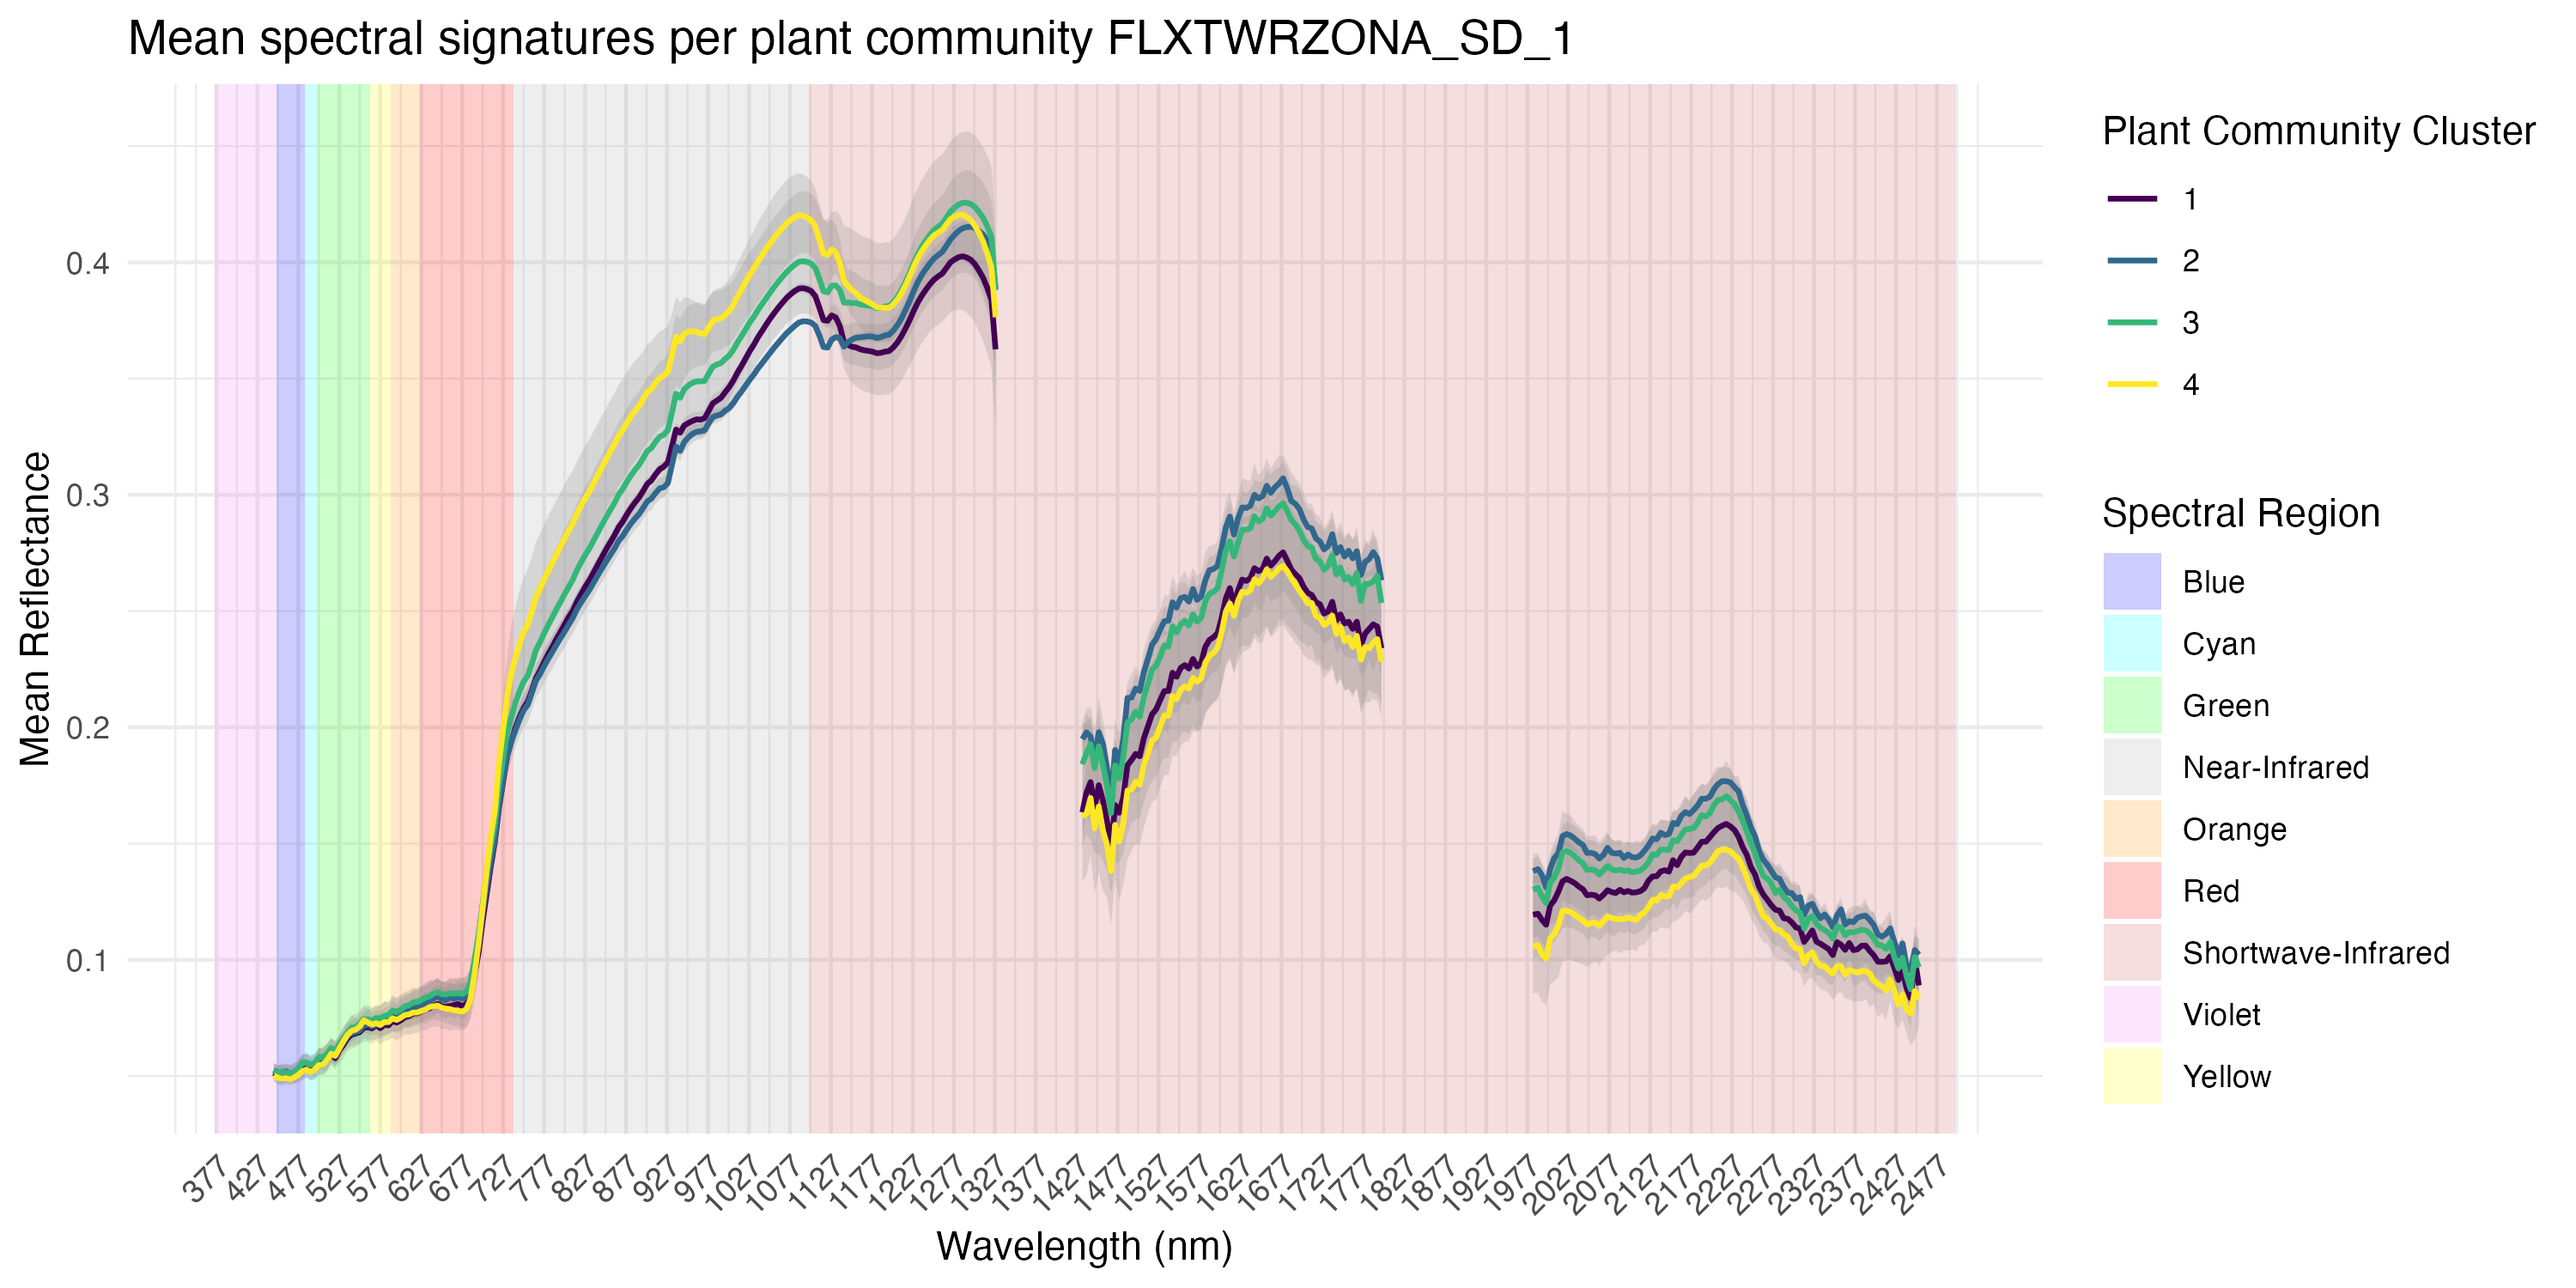
\includegraphics[width=\textwidth]{Figures/spectral_signatures/FLXTWRZONA_SD_1_mean_signature_plot_plant_community.png}
    \caption{}
    \label{fig:mss_pc_flxtwrzonasd1}
  \end{subfigure}

  \caption{Spectral signature plot \ref{fig:ss_pc_flxtwrzonasd1} and mean spectral signature plot \ref{fig:mss_pc_flxtwrzonasd1} grouped by plant community cluster for test site FLXTWRZONA\_SD\_1}
  \label{fig:group_pc_ht_flxtwrzonasd1}
\end{figure}

\subsection{FLXTWRZONA\_SD\_2}

\begin{figure}[H]
  \centering

  \begin{subfigure}[b]{0.49\textwidth}
    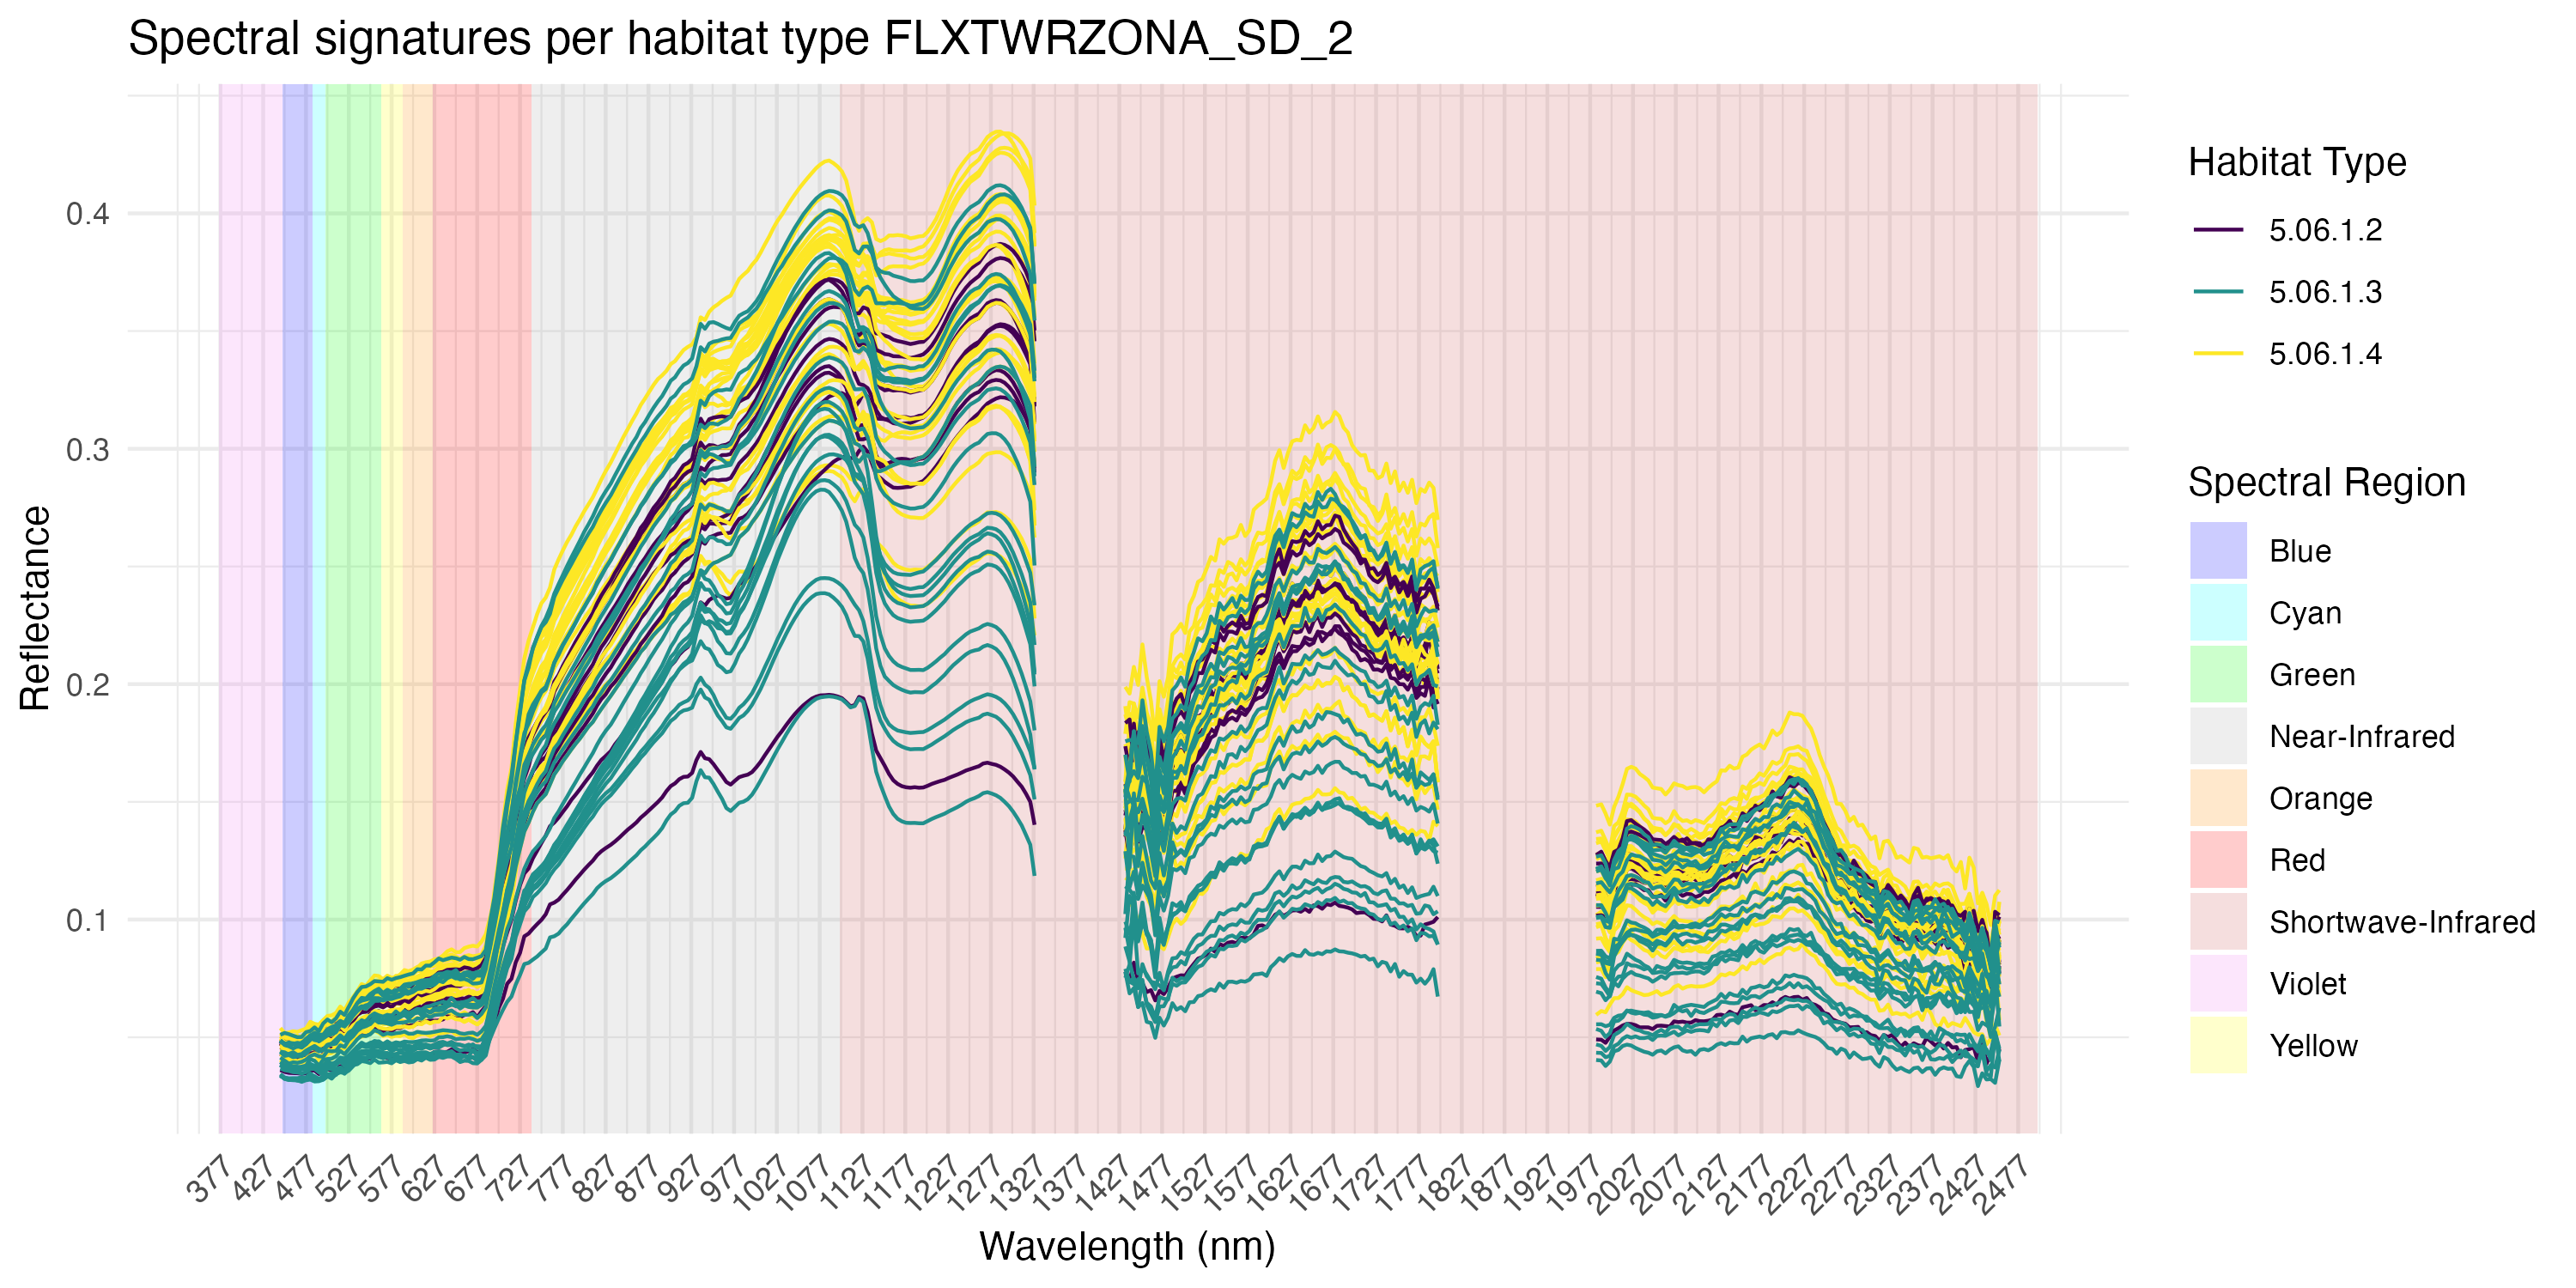
\includegraphics[width=\textwidth]{Figures/spectral_signatures/FLXTWRZONA_SD_2_signature_plot_habitat.png}
    \caption{}
    \label{fig:ss_ht_flxtwrzonasd2}
  \end{subfigure}
  \hfill
  \begin{subfigure}[b]{0.49\textwidth}
    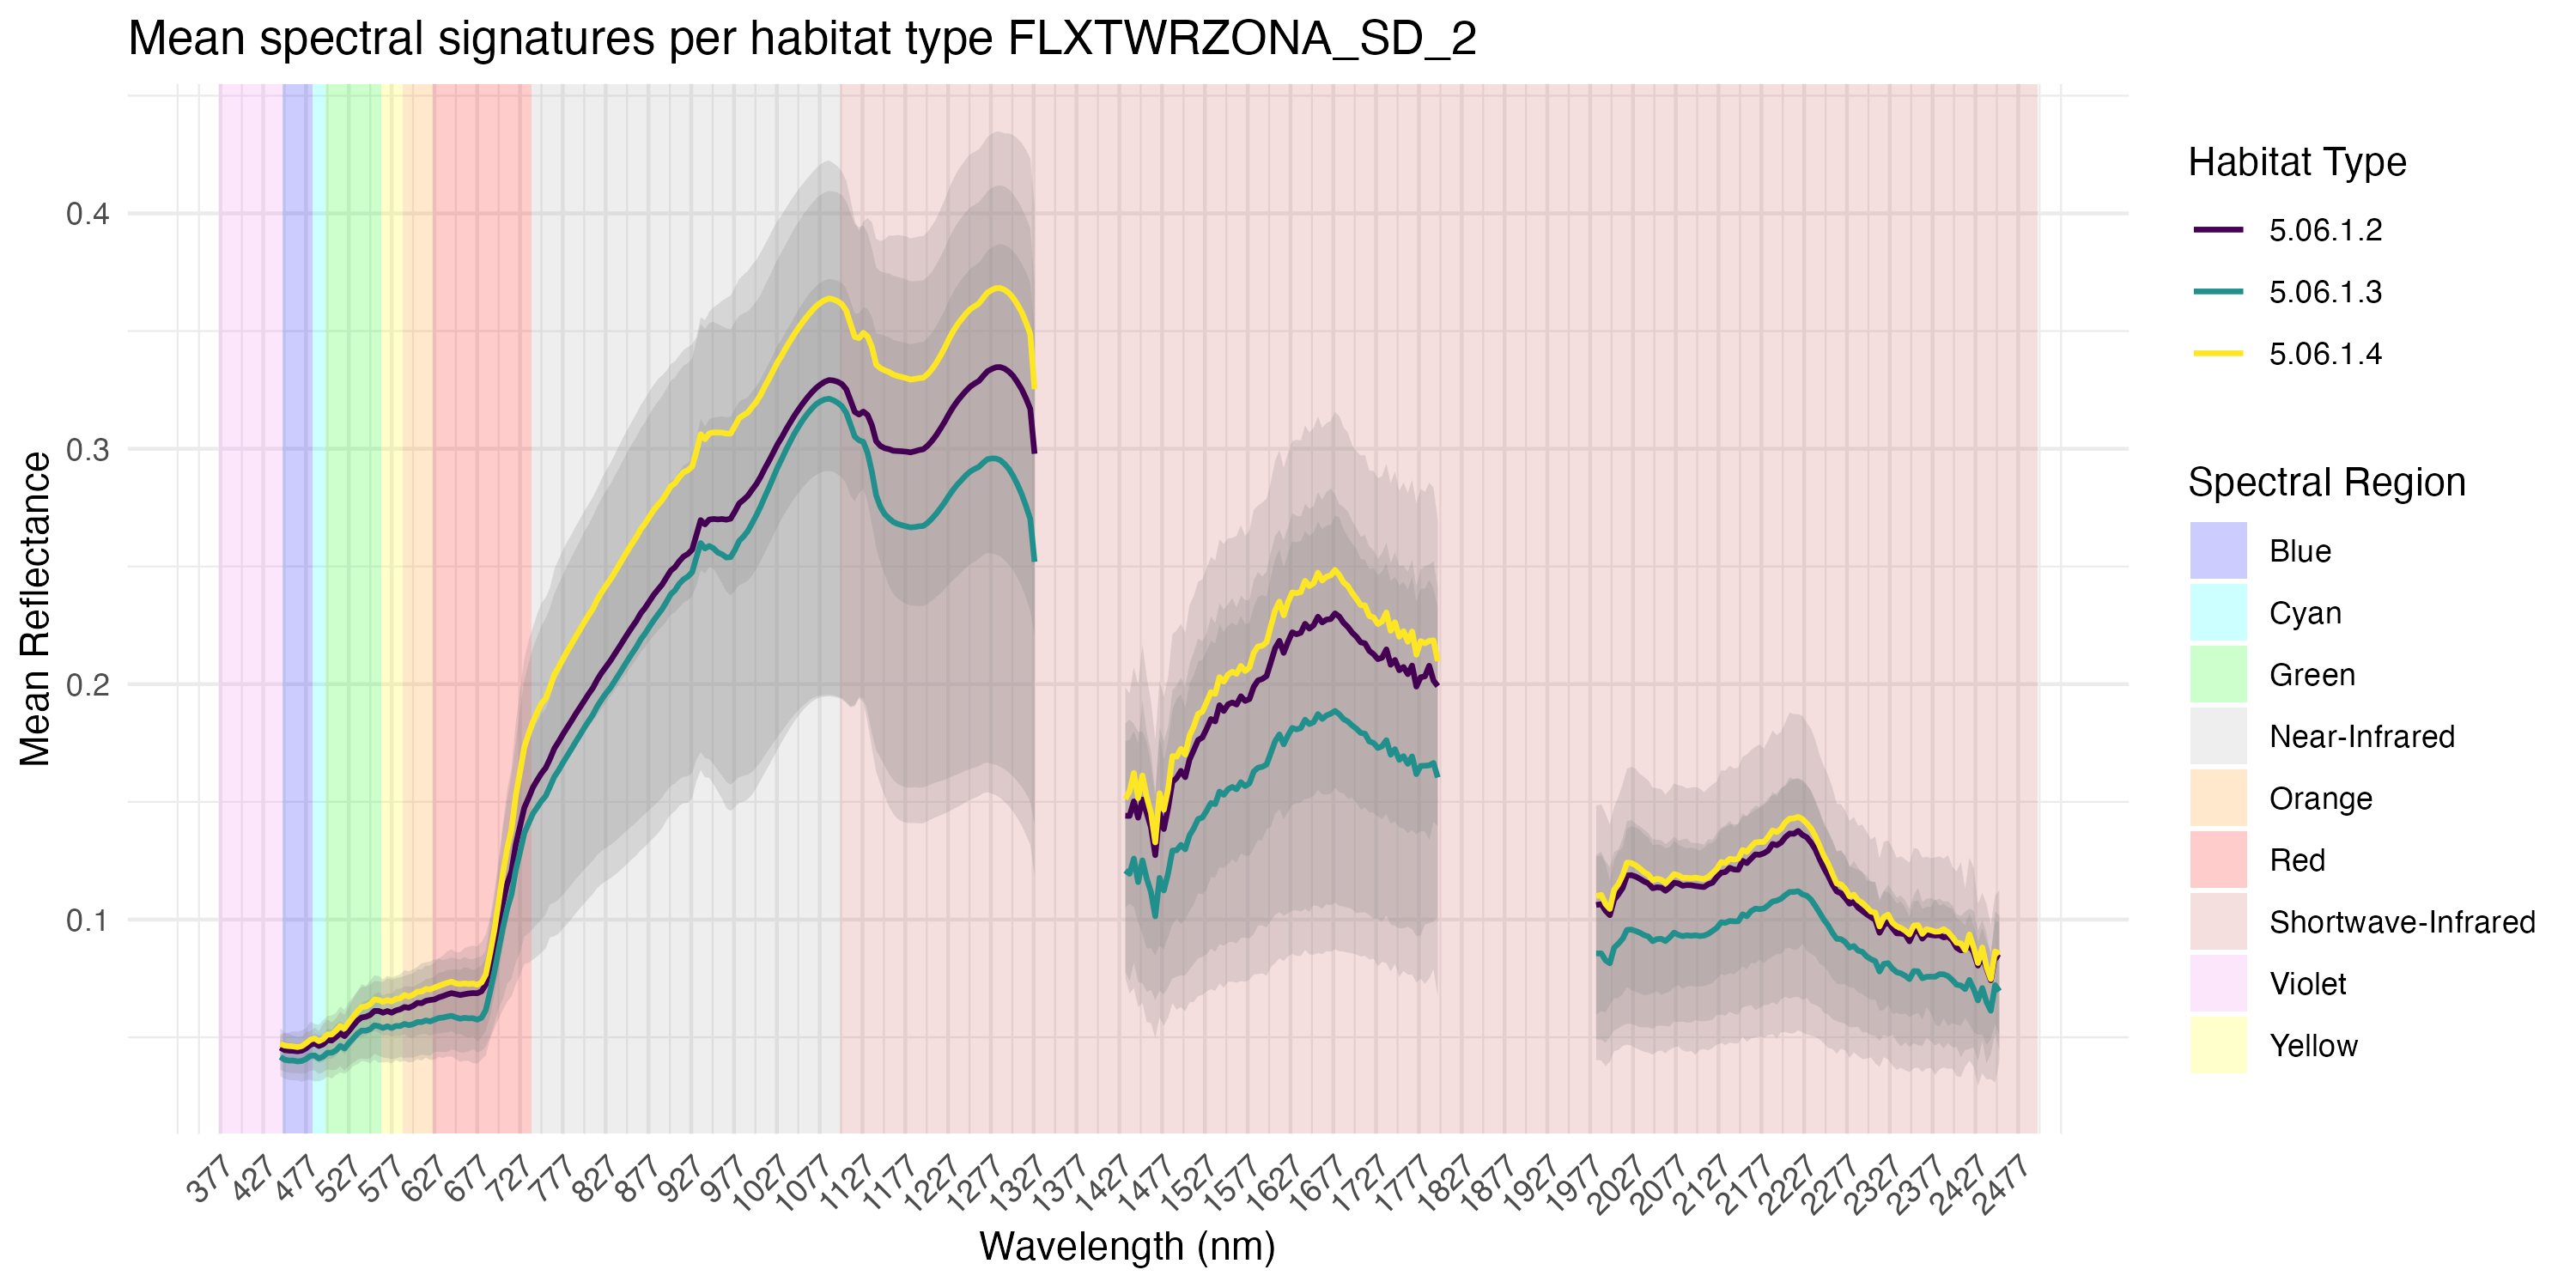
\includegraphics[width=\textwidth]{Figures/spectral_signatures/FLXTWRZONA_SD_2_mean_signature_plot_habitat.png}
    \caption{}
    \label{fig:mss_ht_flxtwrzonasd2}
  \end{subfigure}

  \caption{Spectral signature plot \ref{fig:ss_ht_flxtwrzonasd2} and mean spectral signature plot \ref{fig:mss_ht_flxtwrzonasd2} grouped by habitat type for test site FLXTWRZONA\_SD\_2}
  \label{fig:group_ss_ht_flxtwrzonasd2}
\end{figure}

\begin{figure}[H]
  \centering

  \begin{subfigure}[b]{0.49\textwidth}
    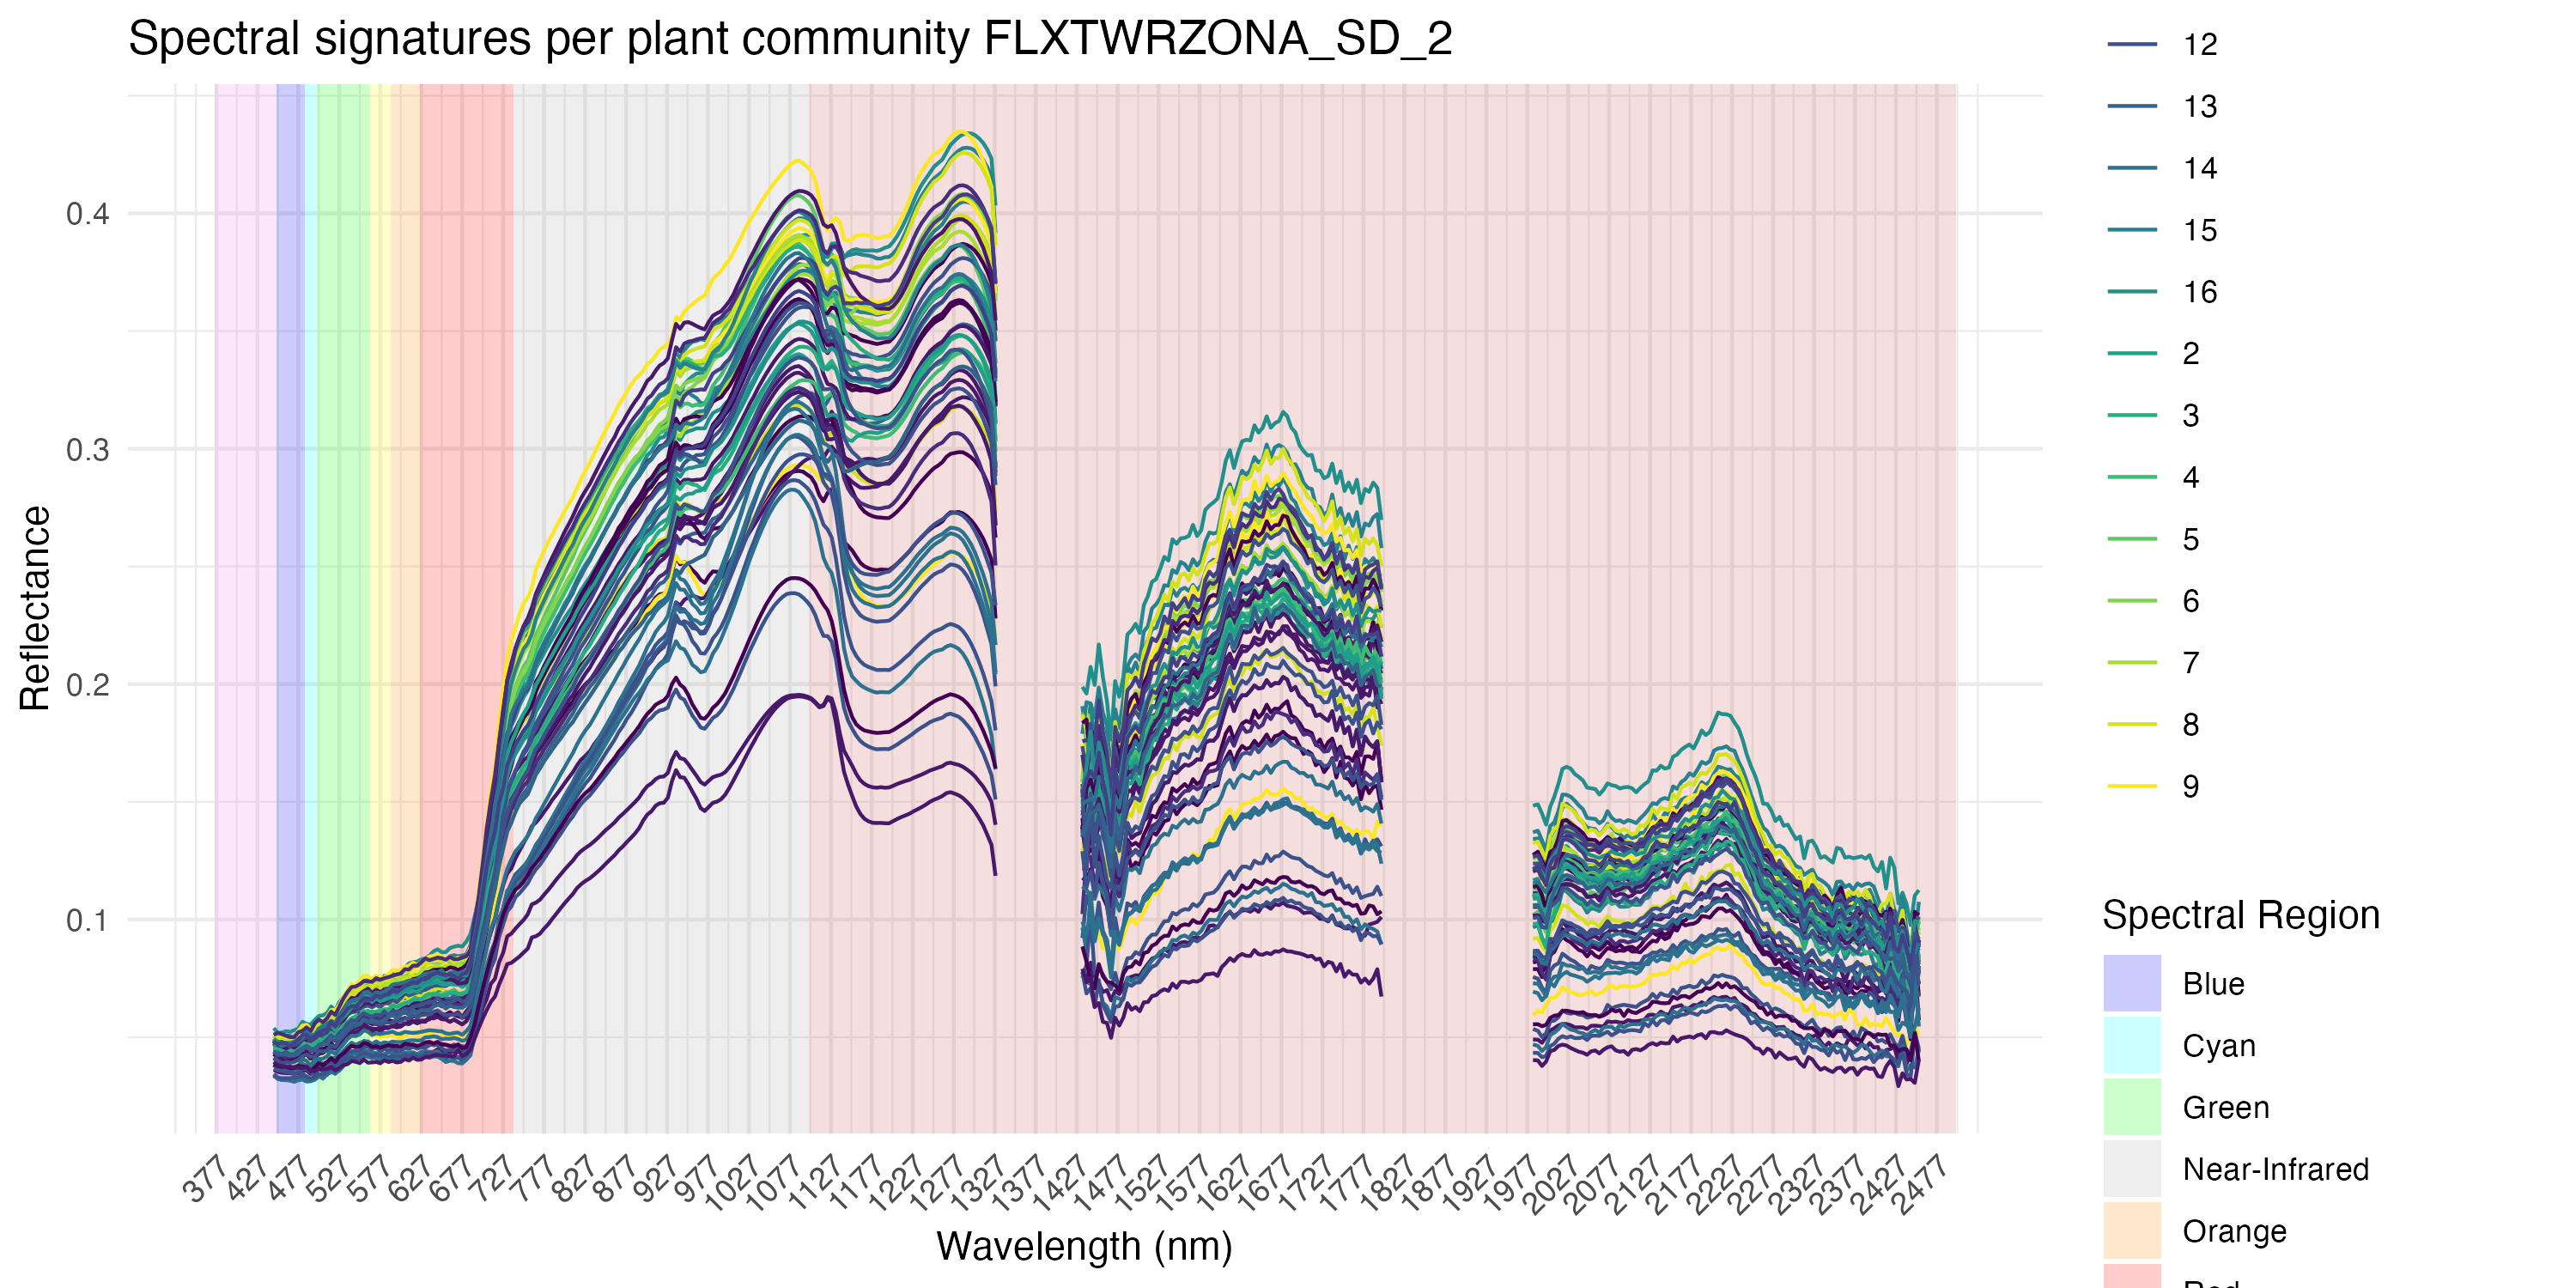
\includegraphics[width=\textwidth]{Figures/spectral_signatures/FLXTWRZONA_SD_2_signature_plot_plant_community.png}
    \caption{}
    \label{fig:ss_pc_flxtwrzonasd2}
  \end{subfigure}
  \hfill
  \begin{subfigure}[b]{0.49\textwidth}
    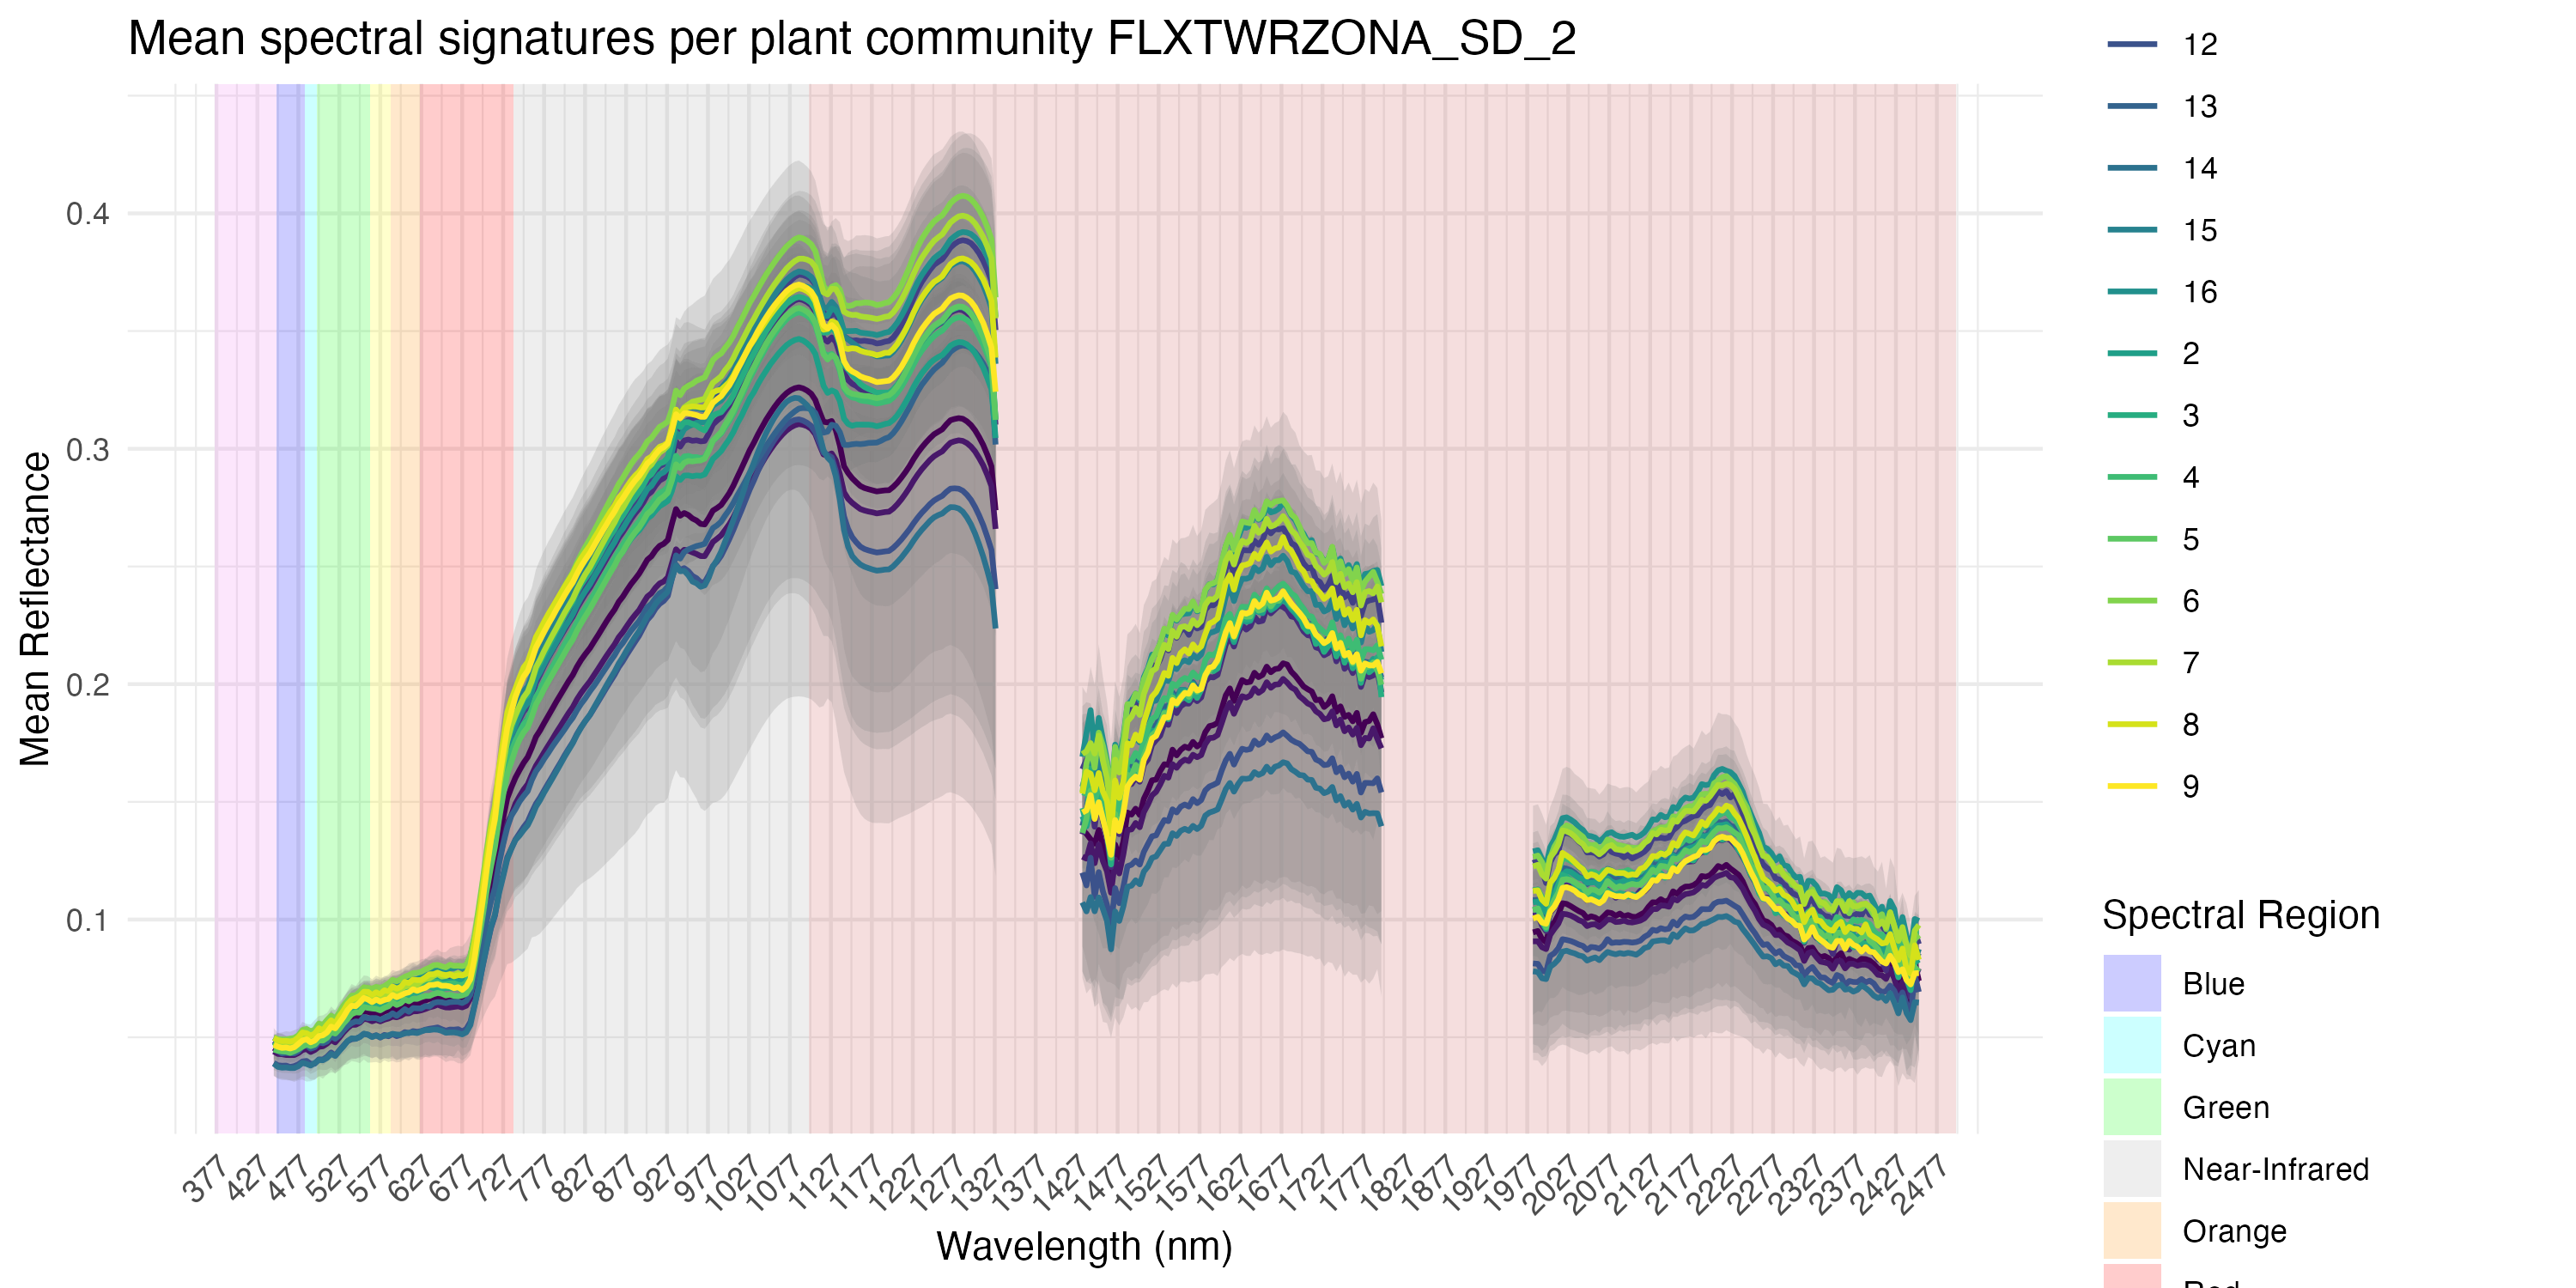
\includegraphics[width=\textwidth]{Figures/spectral_signatures/FLXTWRZONA_SD_2_mean_signature_plot_plant_community.png}
    \caption{}
    \label{fig:mss_pc_flxtwrzonasd2}
  \end{subfigure}

  \caption{Spectral signature plot \ref{fig:ss_pc_flxtwrzonasd2} and mean spectral signature plot \ref{fig:mss_pc_flxtwrzonasd2} grouped by plant community cluster for test site FLXTWRZONA\_SD\_2}
  \label{fig:group_pc_ht_flxtwrzonasd2}
\end{figure}

\subsection{FLXTWRZONA\_SD\_3}

\begin{figure}[H]
  \centering

  \begin{subfigure}[b]{0.49\textwidth}
    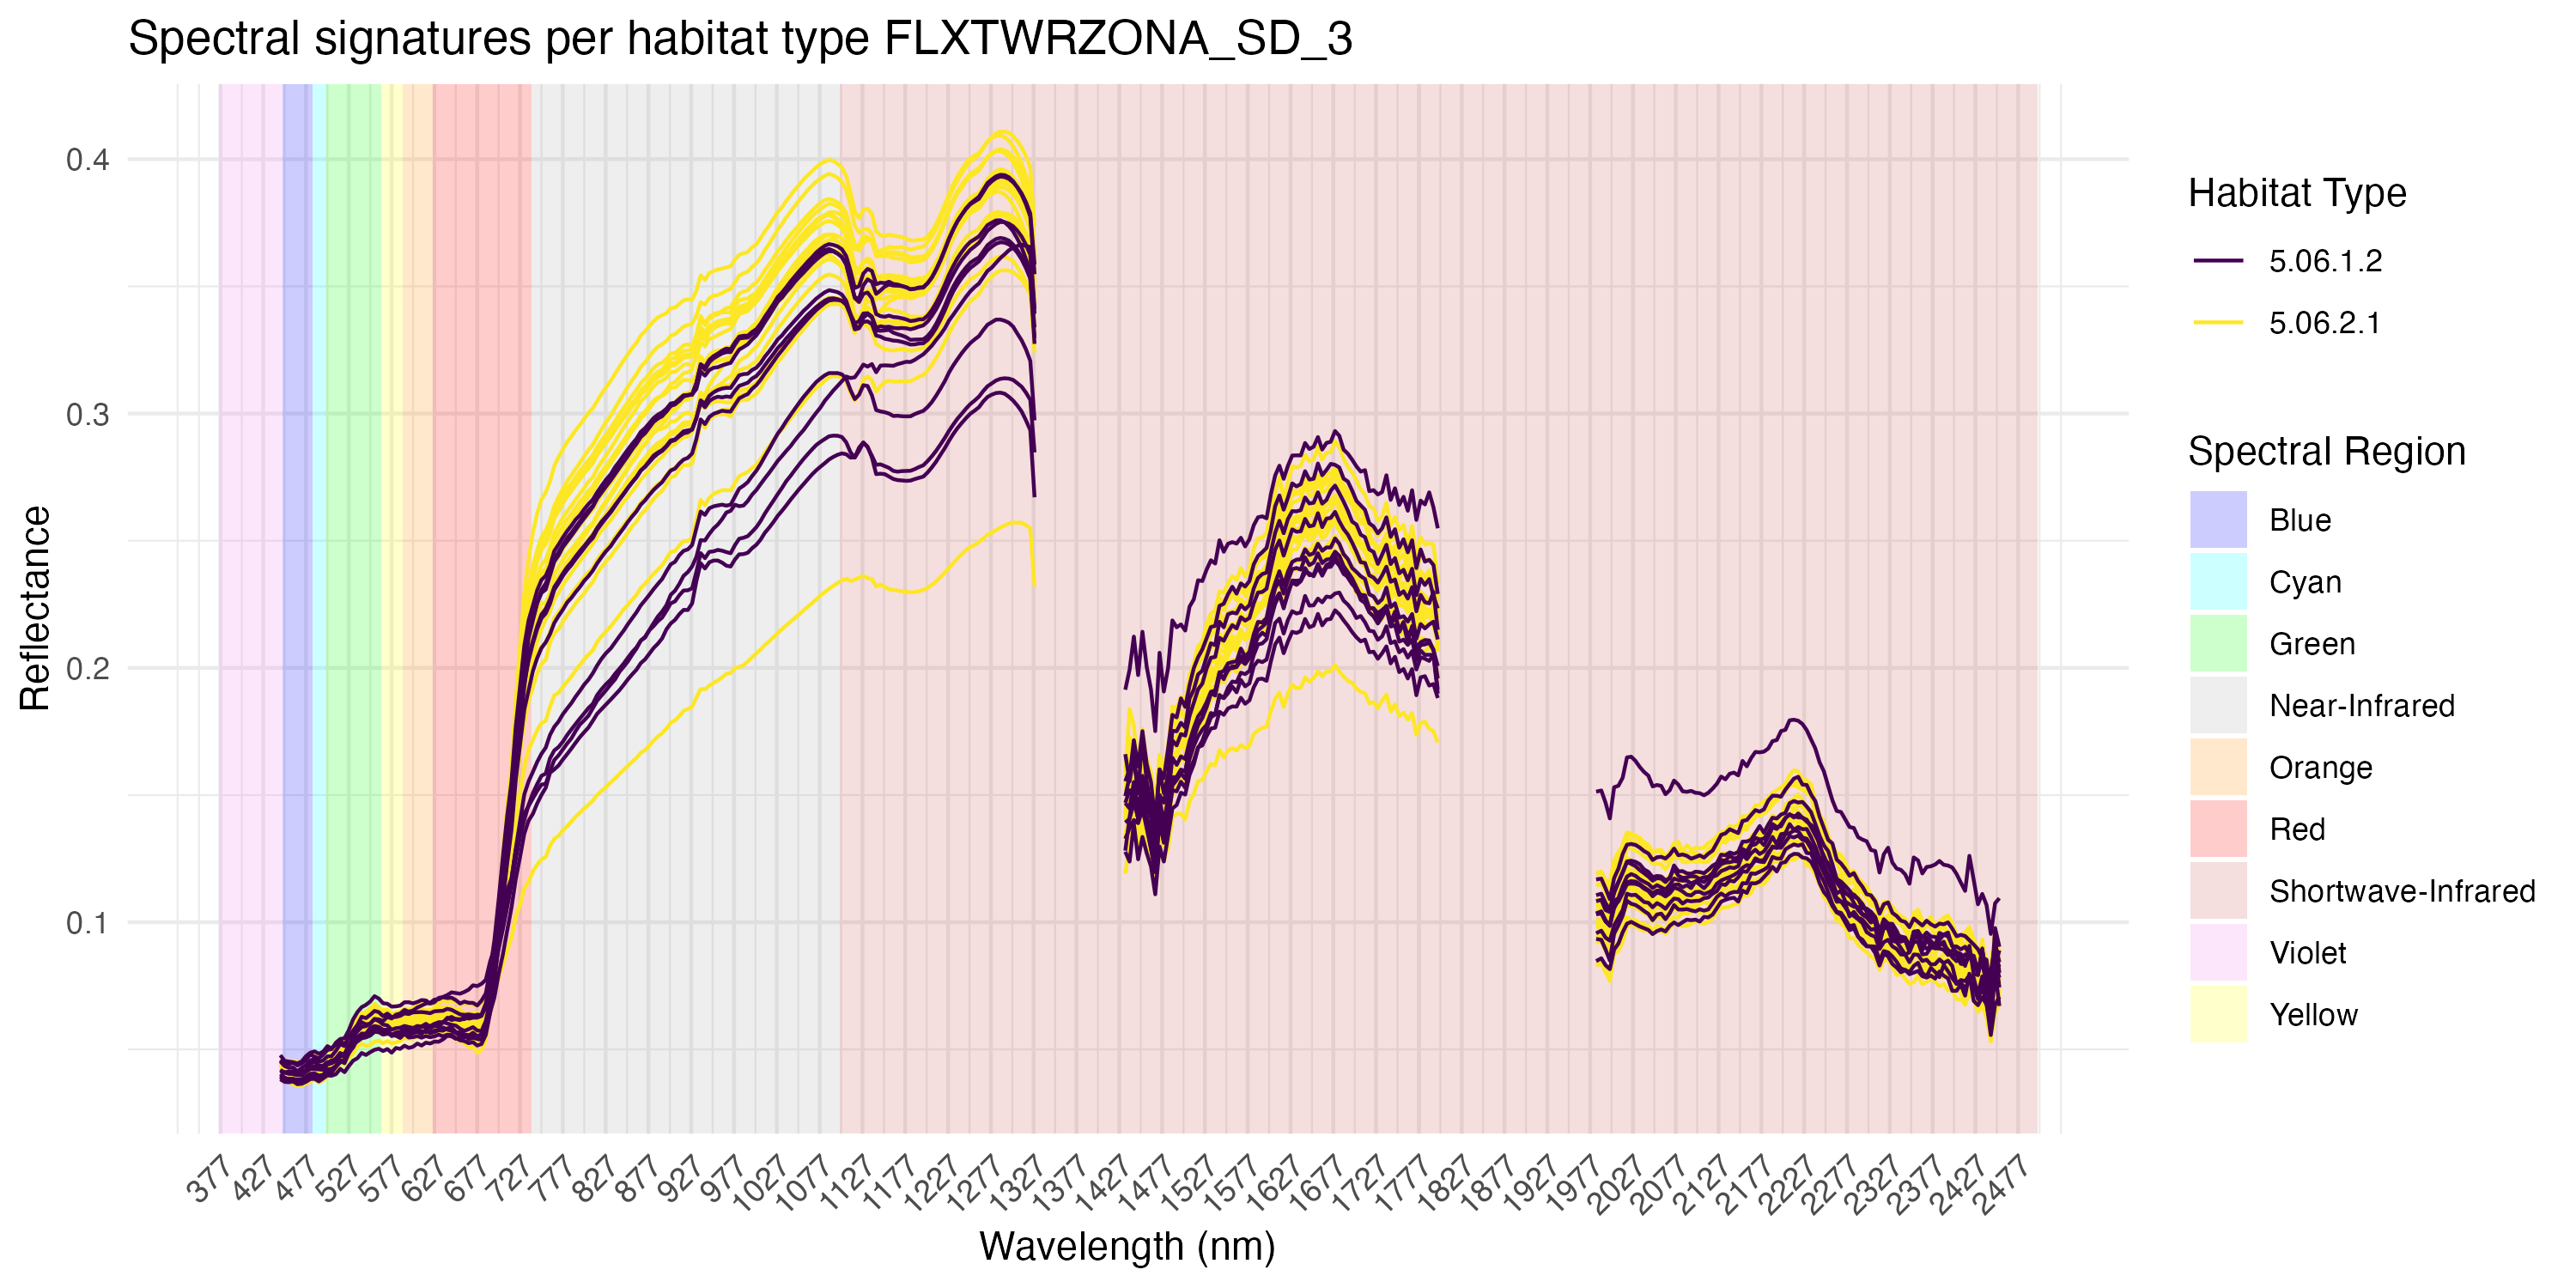
\includegraphics[width=\textwidth]{Figures/spectral_signatures/FLXTWRZONA_SD_3_signature_plot_habitat.png}
    \caption{}
    \label{fig:ss_ht_flxtwrzonasd3}
  \end{subfigure}
  \hfill
  \begin{subfigure}[b]{0.49\textwidth}
    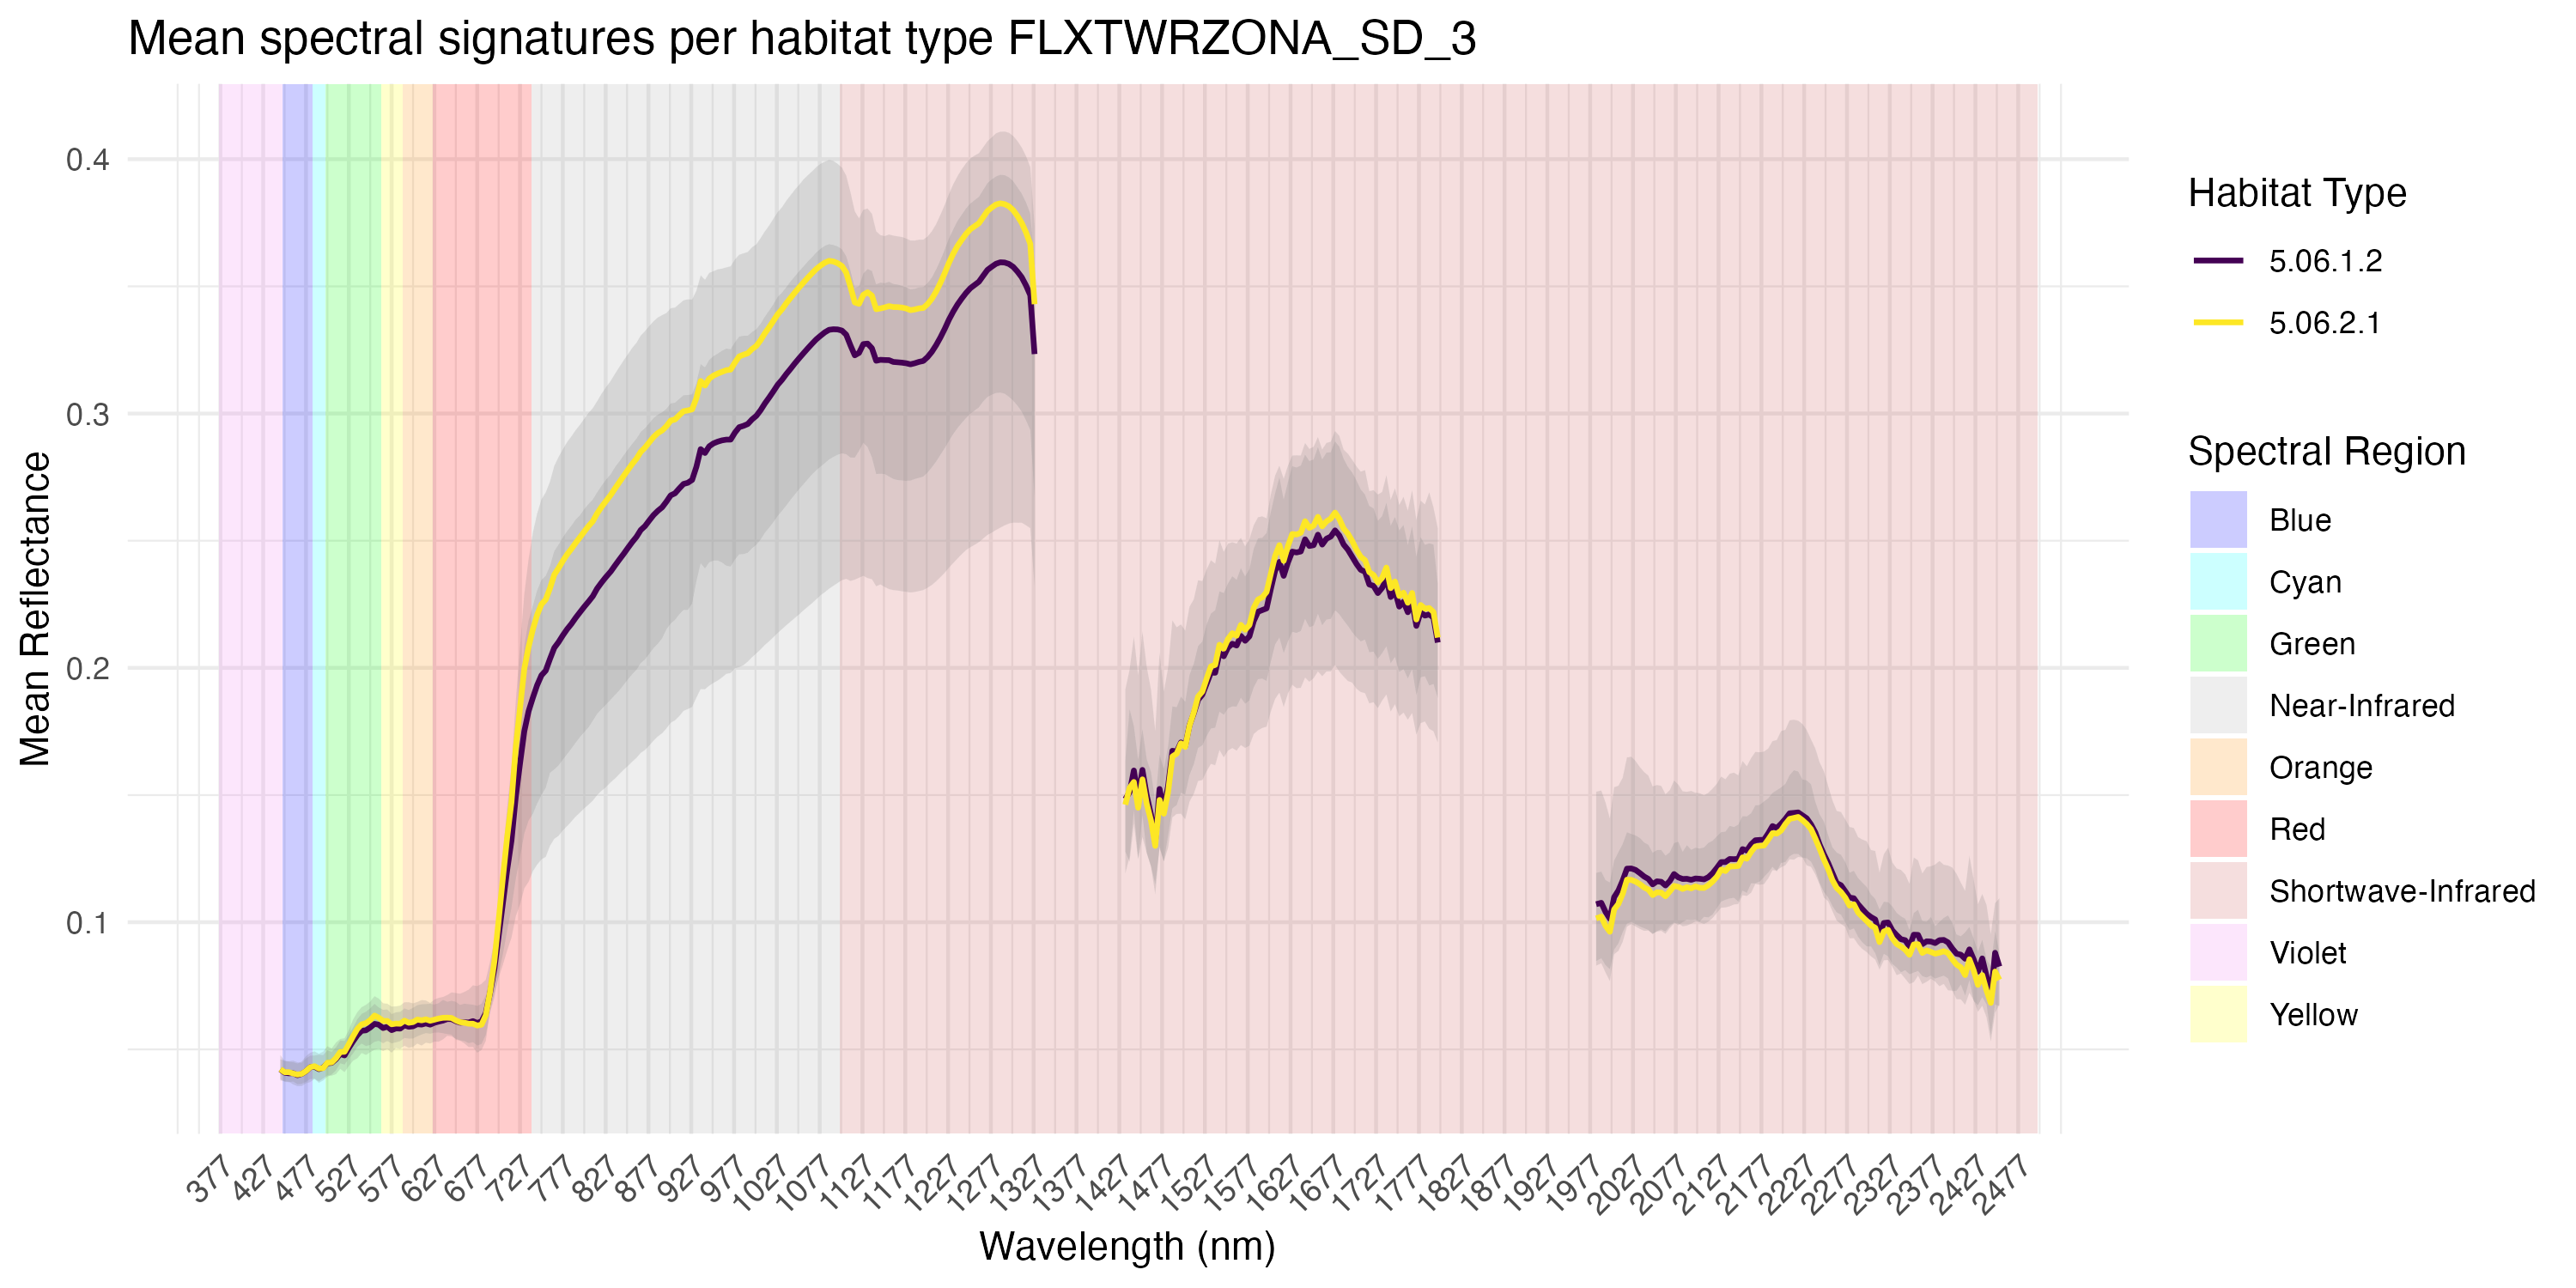
\includegraphics[width=\textwidth]{Figures/spectral_signatures/FLXTWRZONA_SD_3_mean_signature_plot_habitat.png}
    \caption{}
    \label{fig:mss_ht_flxtwrzonasd3}
  \end{subfigure}

  \caption{Spectral signature plot \ref{fig:ss_ht_flxtwrzonasd3} and mean spectral signature plot \ref{fig:mss_ht_flxtwrzonasd3} grouped by habitat type for test site FLXTWRZONA\_SD\_3}
  \label{fig:group_ss_ht_flxtwrzonasd3}
\end{figure}

\begin{figure}[H]
  \centering

  \begin{subfigure}[b]{0.49\textwidth}
    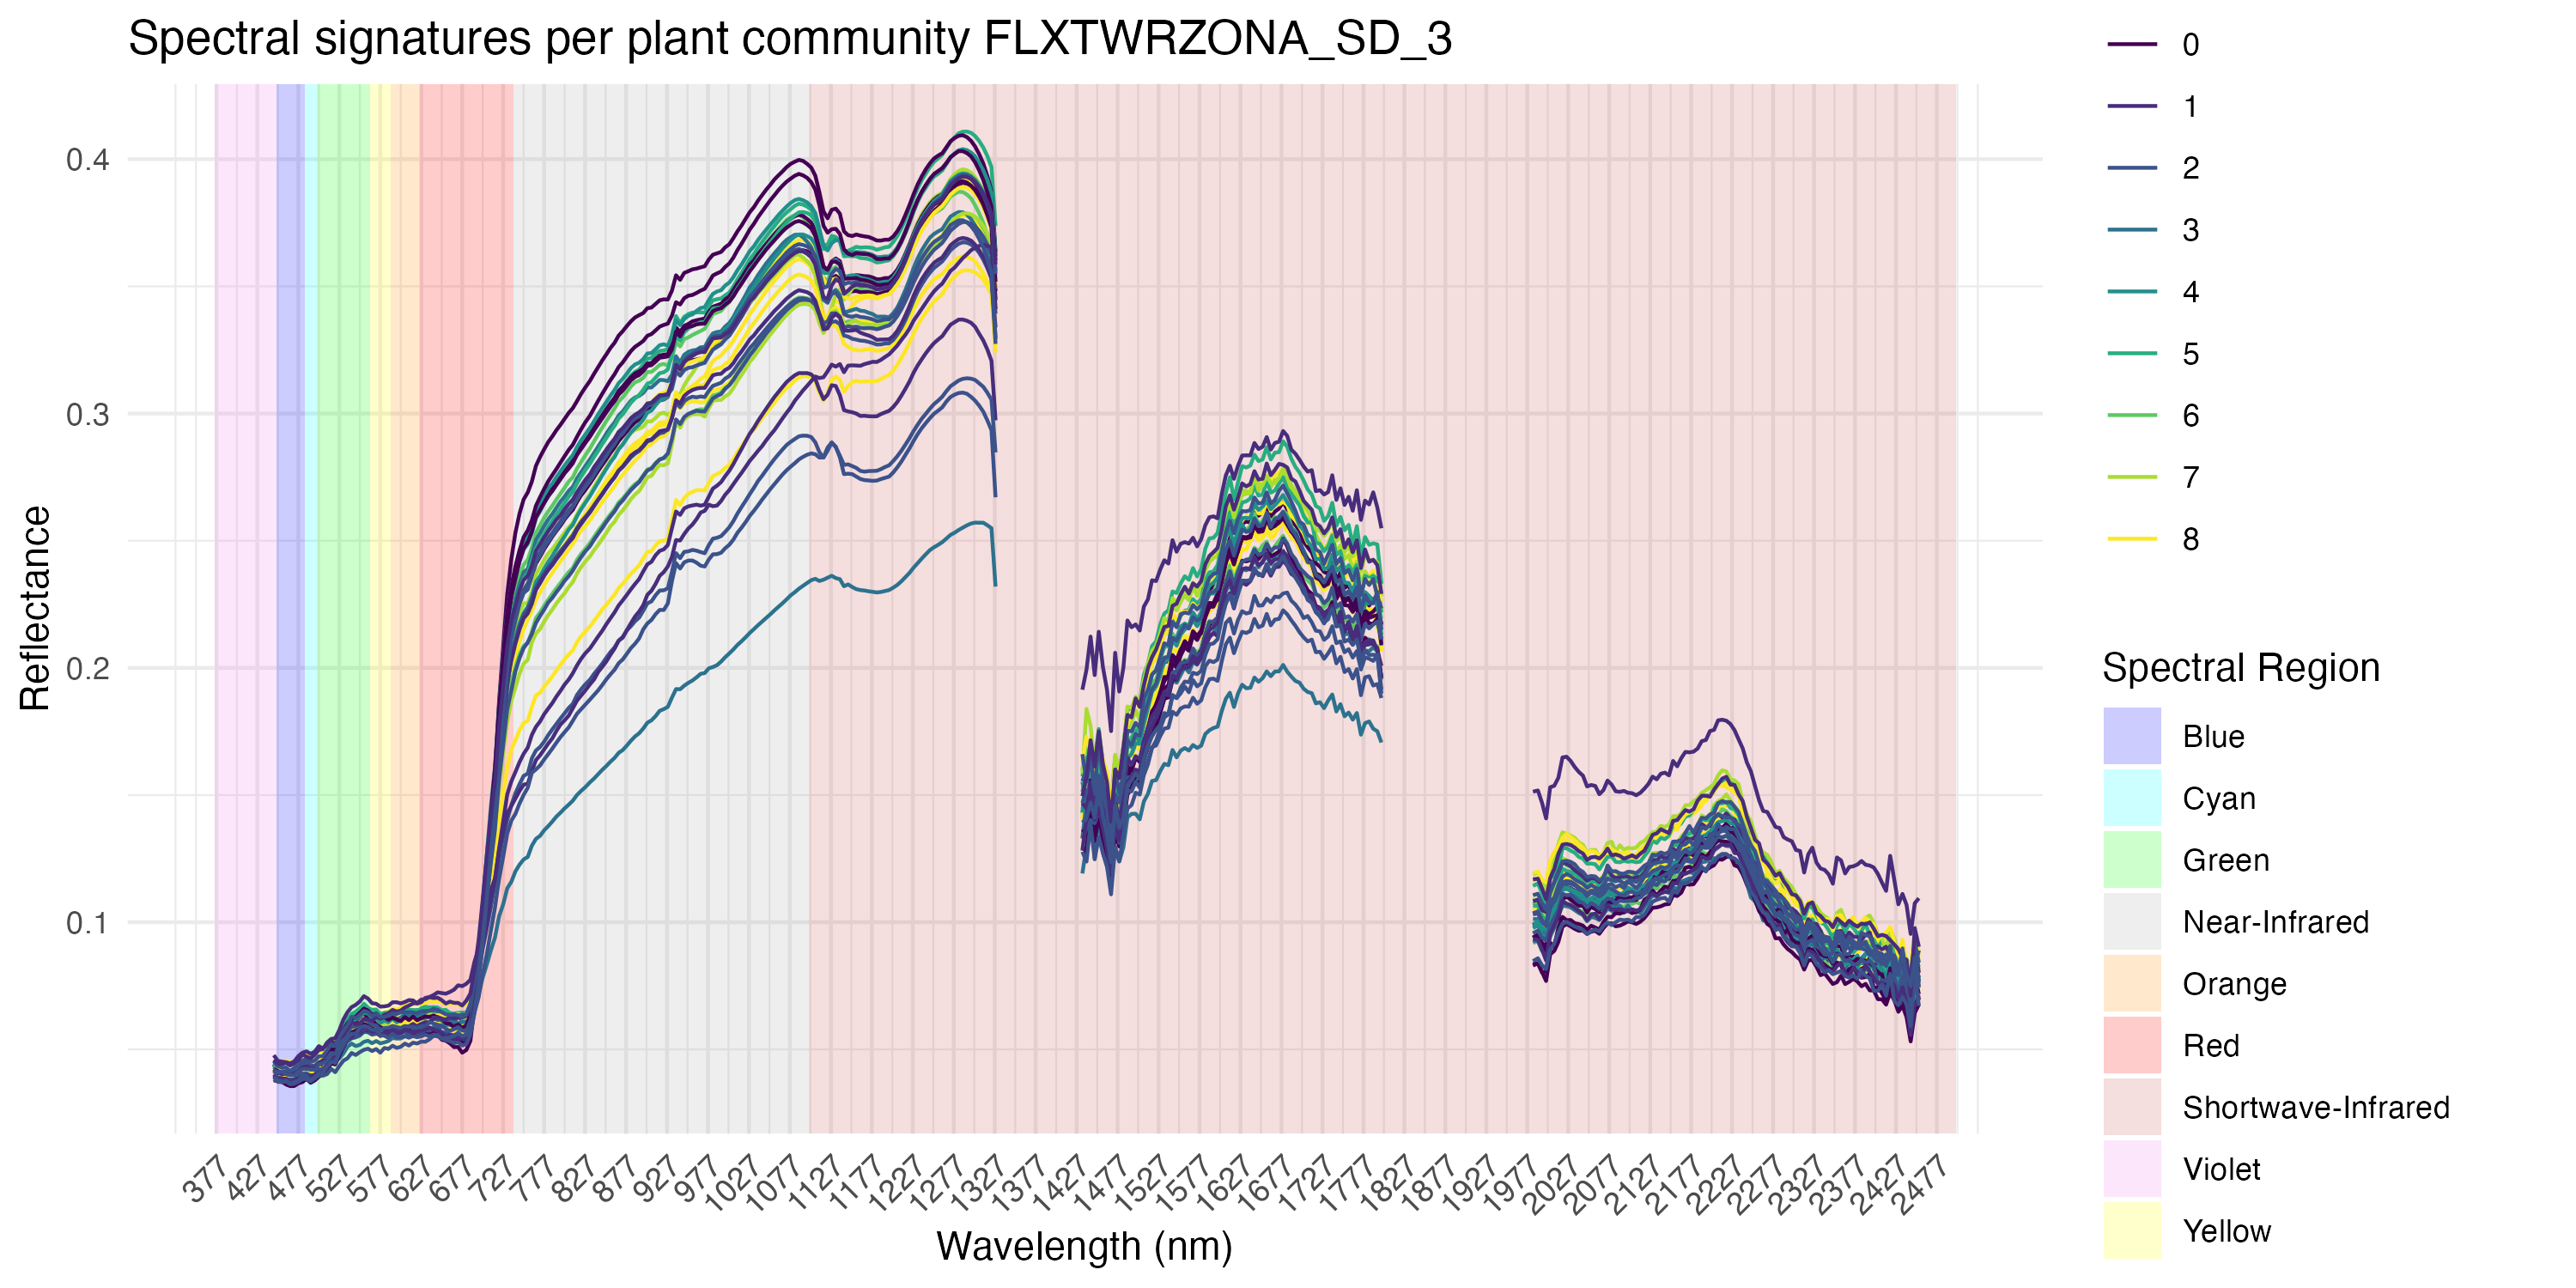
\includegraphics[width=\textwidth]{Figures/spectral_signatures/FLXTWRZONA_SD_3_signature_plot_plant_community.png}
    \caption{}
    \label{fig:ss_pc_flxtwrzonasd3}
  \end{subfigure}
  \hfill
  \begin{subfigure}[b]{0.49\textwidth}
    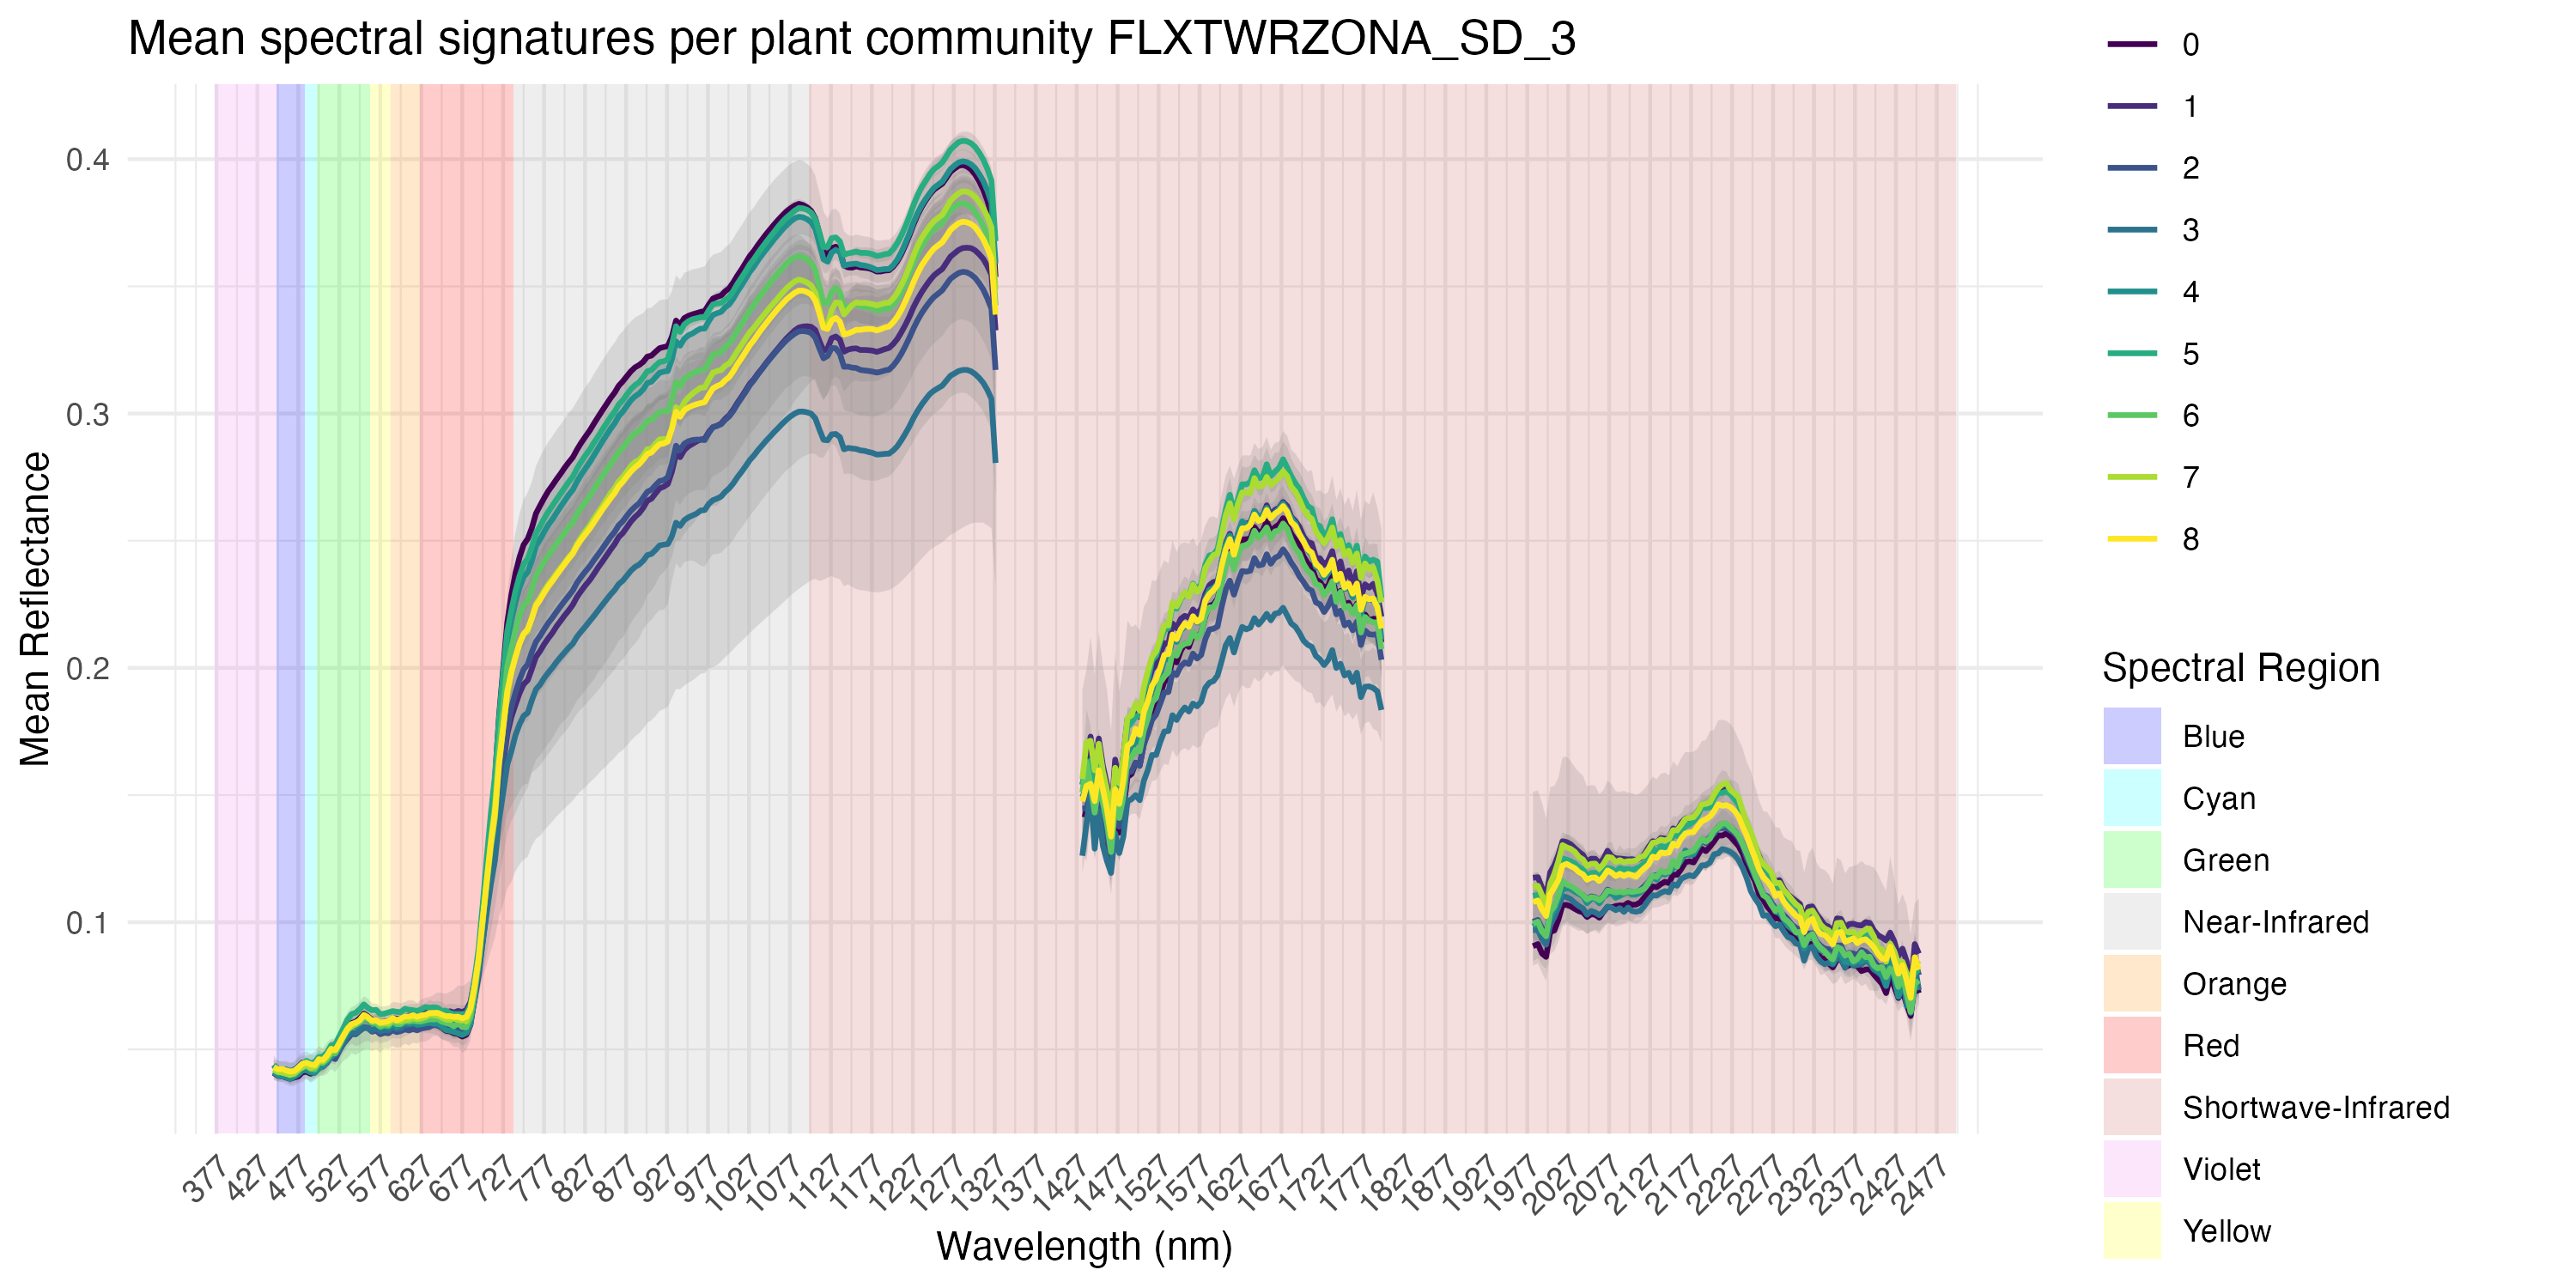
\includegraphics[width=\textwidth]{Figures/spectral_signatures/FLXTWRZONA_SD_3_mean_signature_plot_plant_community.png}
    \caption{}
    \label{fig:mss_pc_flxtwrzonasd3}
  \end{subfigure}

  \caption{Spectral signature plot \ref{fig:ss_pc_flxtwrzonasd3} and mean spectral signature plot \ref{fig:mss_pc_flxtwrzonasd3} grouped by plant community cluster for test site FLXTWRZONA\_SD\_3}
  \label{fig:group_pc_ht_flxtwrzonasd3}
\end{figure}

\subsection{FLXTWRZONA\_SD\_4}

\begin{figure}[H]
  \centering

  \begin{subfigure}[b]{0.49\textwidth}
    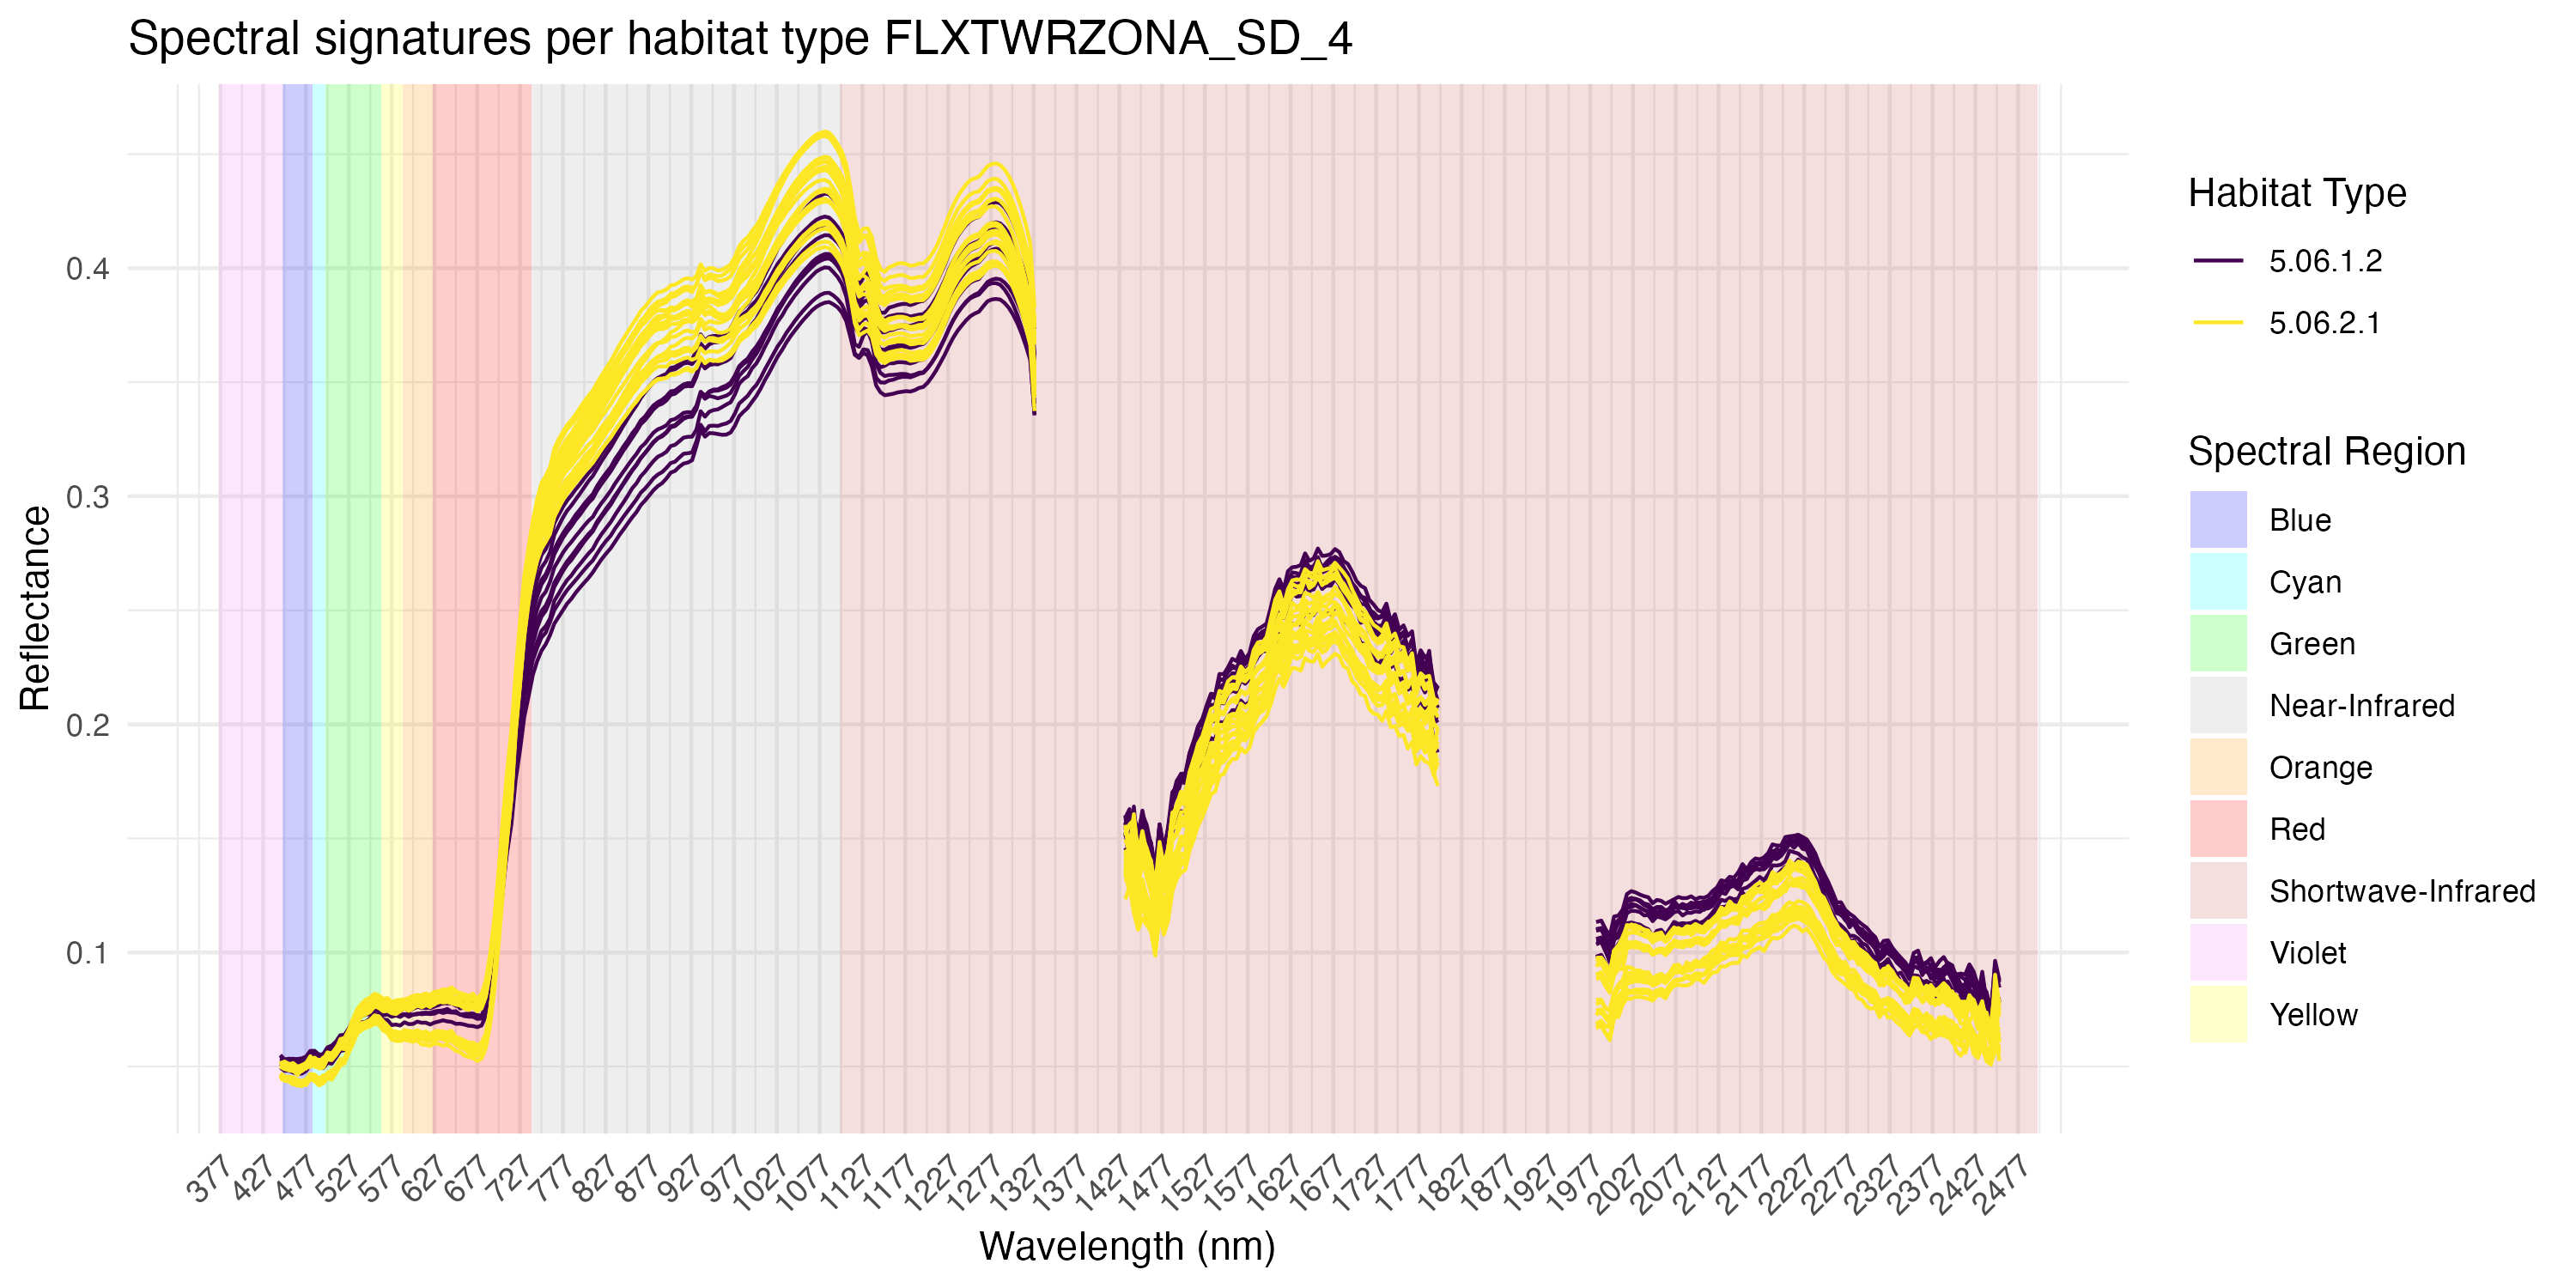
\includegraphics[width=\textwidth]{Figures/spectral_signatures/FLXTWRZONA_SD_4_signature_plot_habitat.png}
    \caption{}
    \label{fig:ss_ht_flxtwrzonasd4}
  \end{subfigure}
  \hfill
  \begin{subfigure}[b]{0.49\textwidth}
    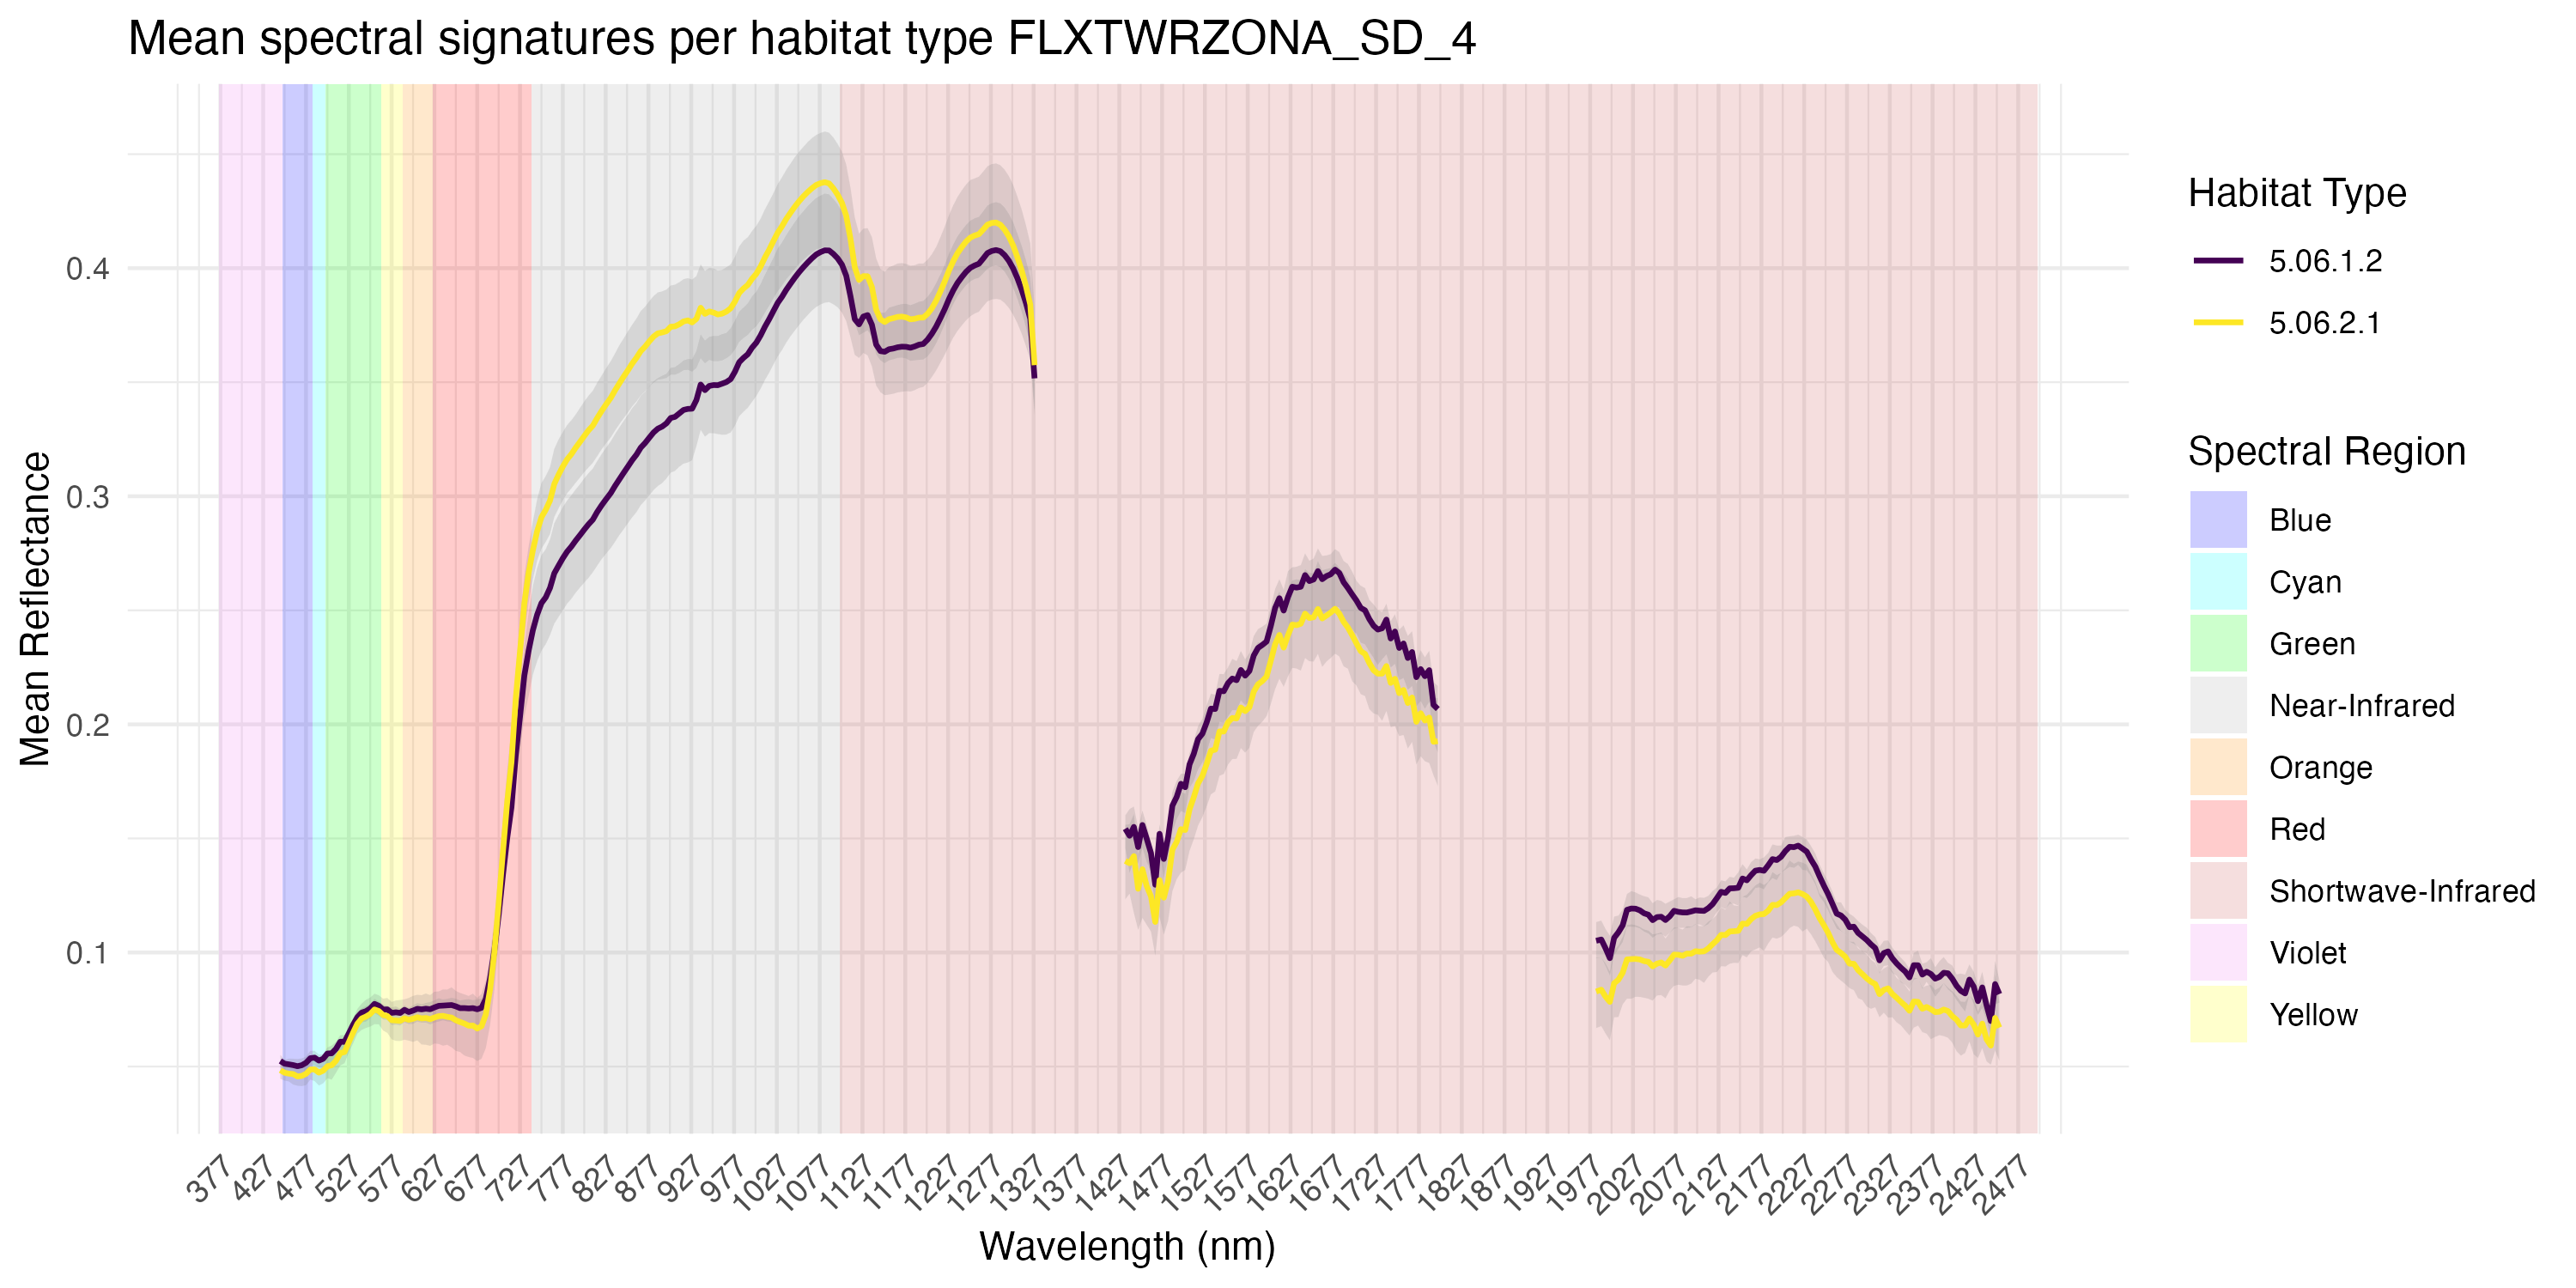
\includegraphics[width=\textwidth]{Figures/spectral_signatures/FLXTWRZONA_SD_4_mean_signature_plot_habitat.png}
    \caption{}
    \label{fig:mss_ht_flxtwrzonasd4}
  \end{subfigure}

  \caption{Spectral signature plot \ref{fig:ss_ht_flxtwrzonasd4} and mean spectral signature plot \ref{fig:mss_ht_flxtwrzonasd4} grouped by habitat type for test site FLXTWRZONA\_SD\_4}
  \label{fig:group_ss_ht_flxtwrzonasd4}
\end{figure}

\begin{figure}[H]
  \centering

  \begin{subfigure}[b]{0.49\textwidth}
    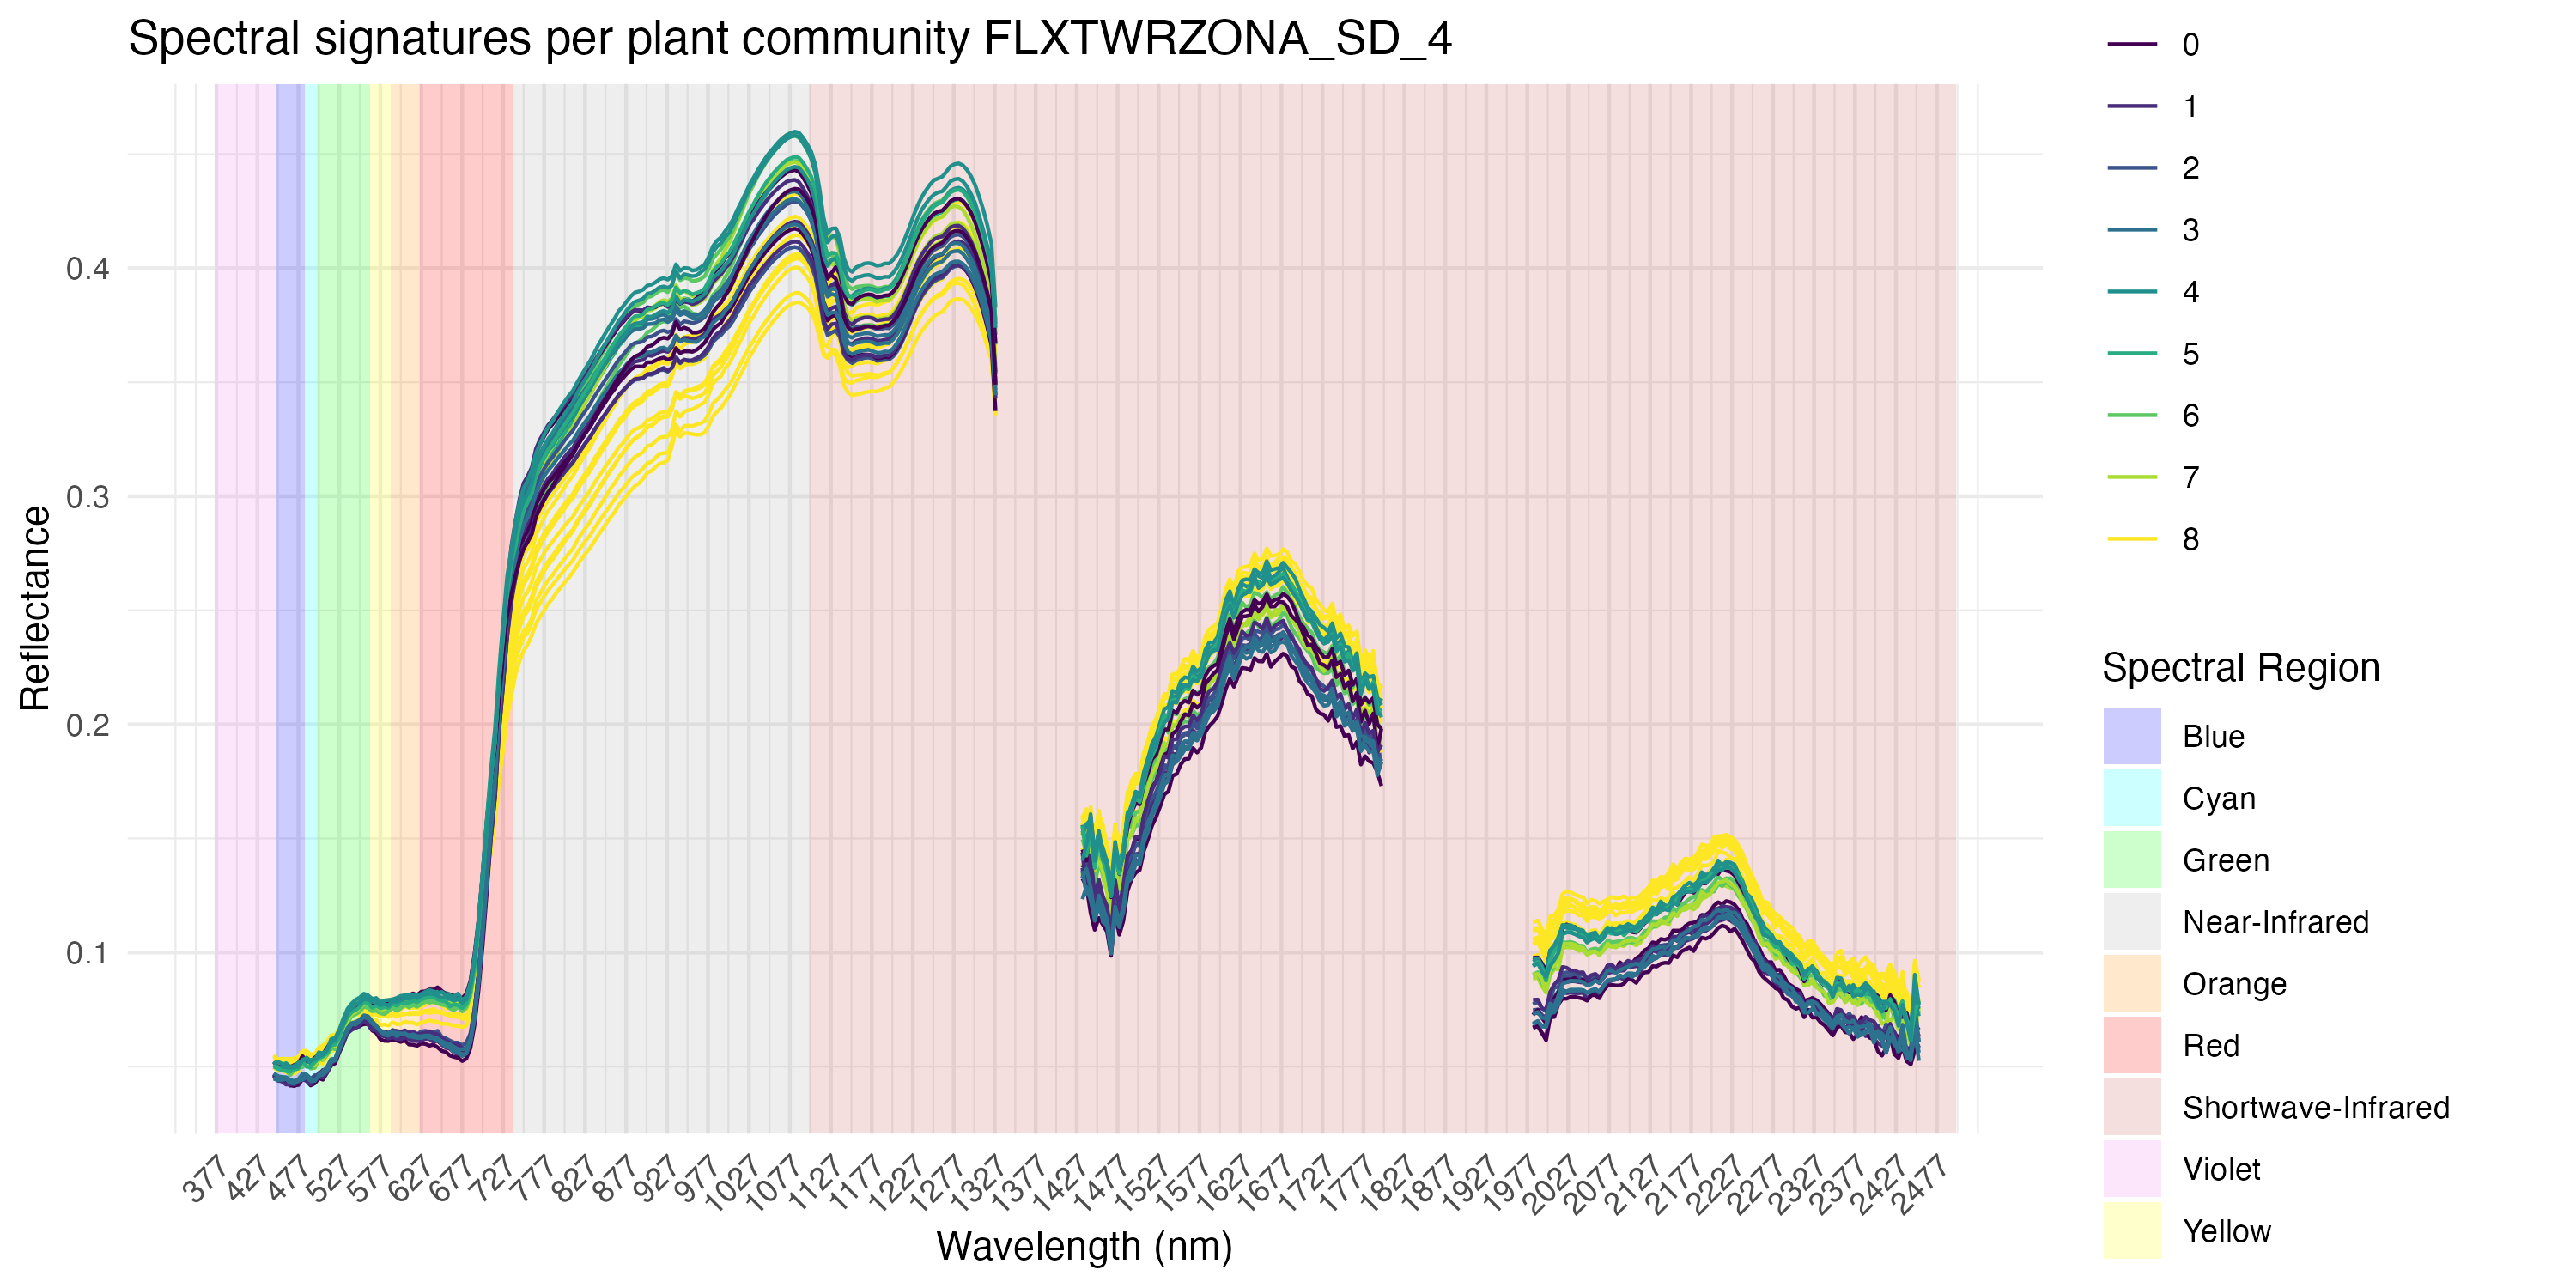
\includegraphics[width=\textwidth]{Figures/spectral_signatures/FLXTWRZONA_SD_4_signature_plot_plant_community.png}
    \caption{}
    \label{fig:ss_pc_flxtwrzonasd4}
  \end{subfigure}
  \hfill
  \begin{subfigure}[b]{0.49\textwidth}
    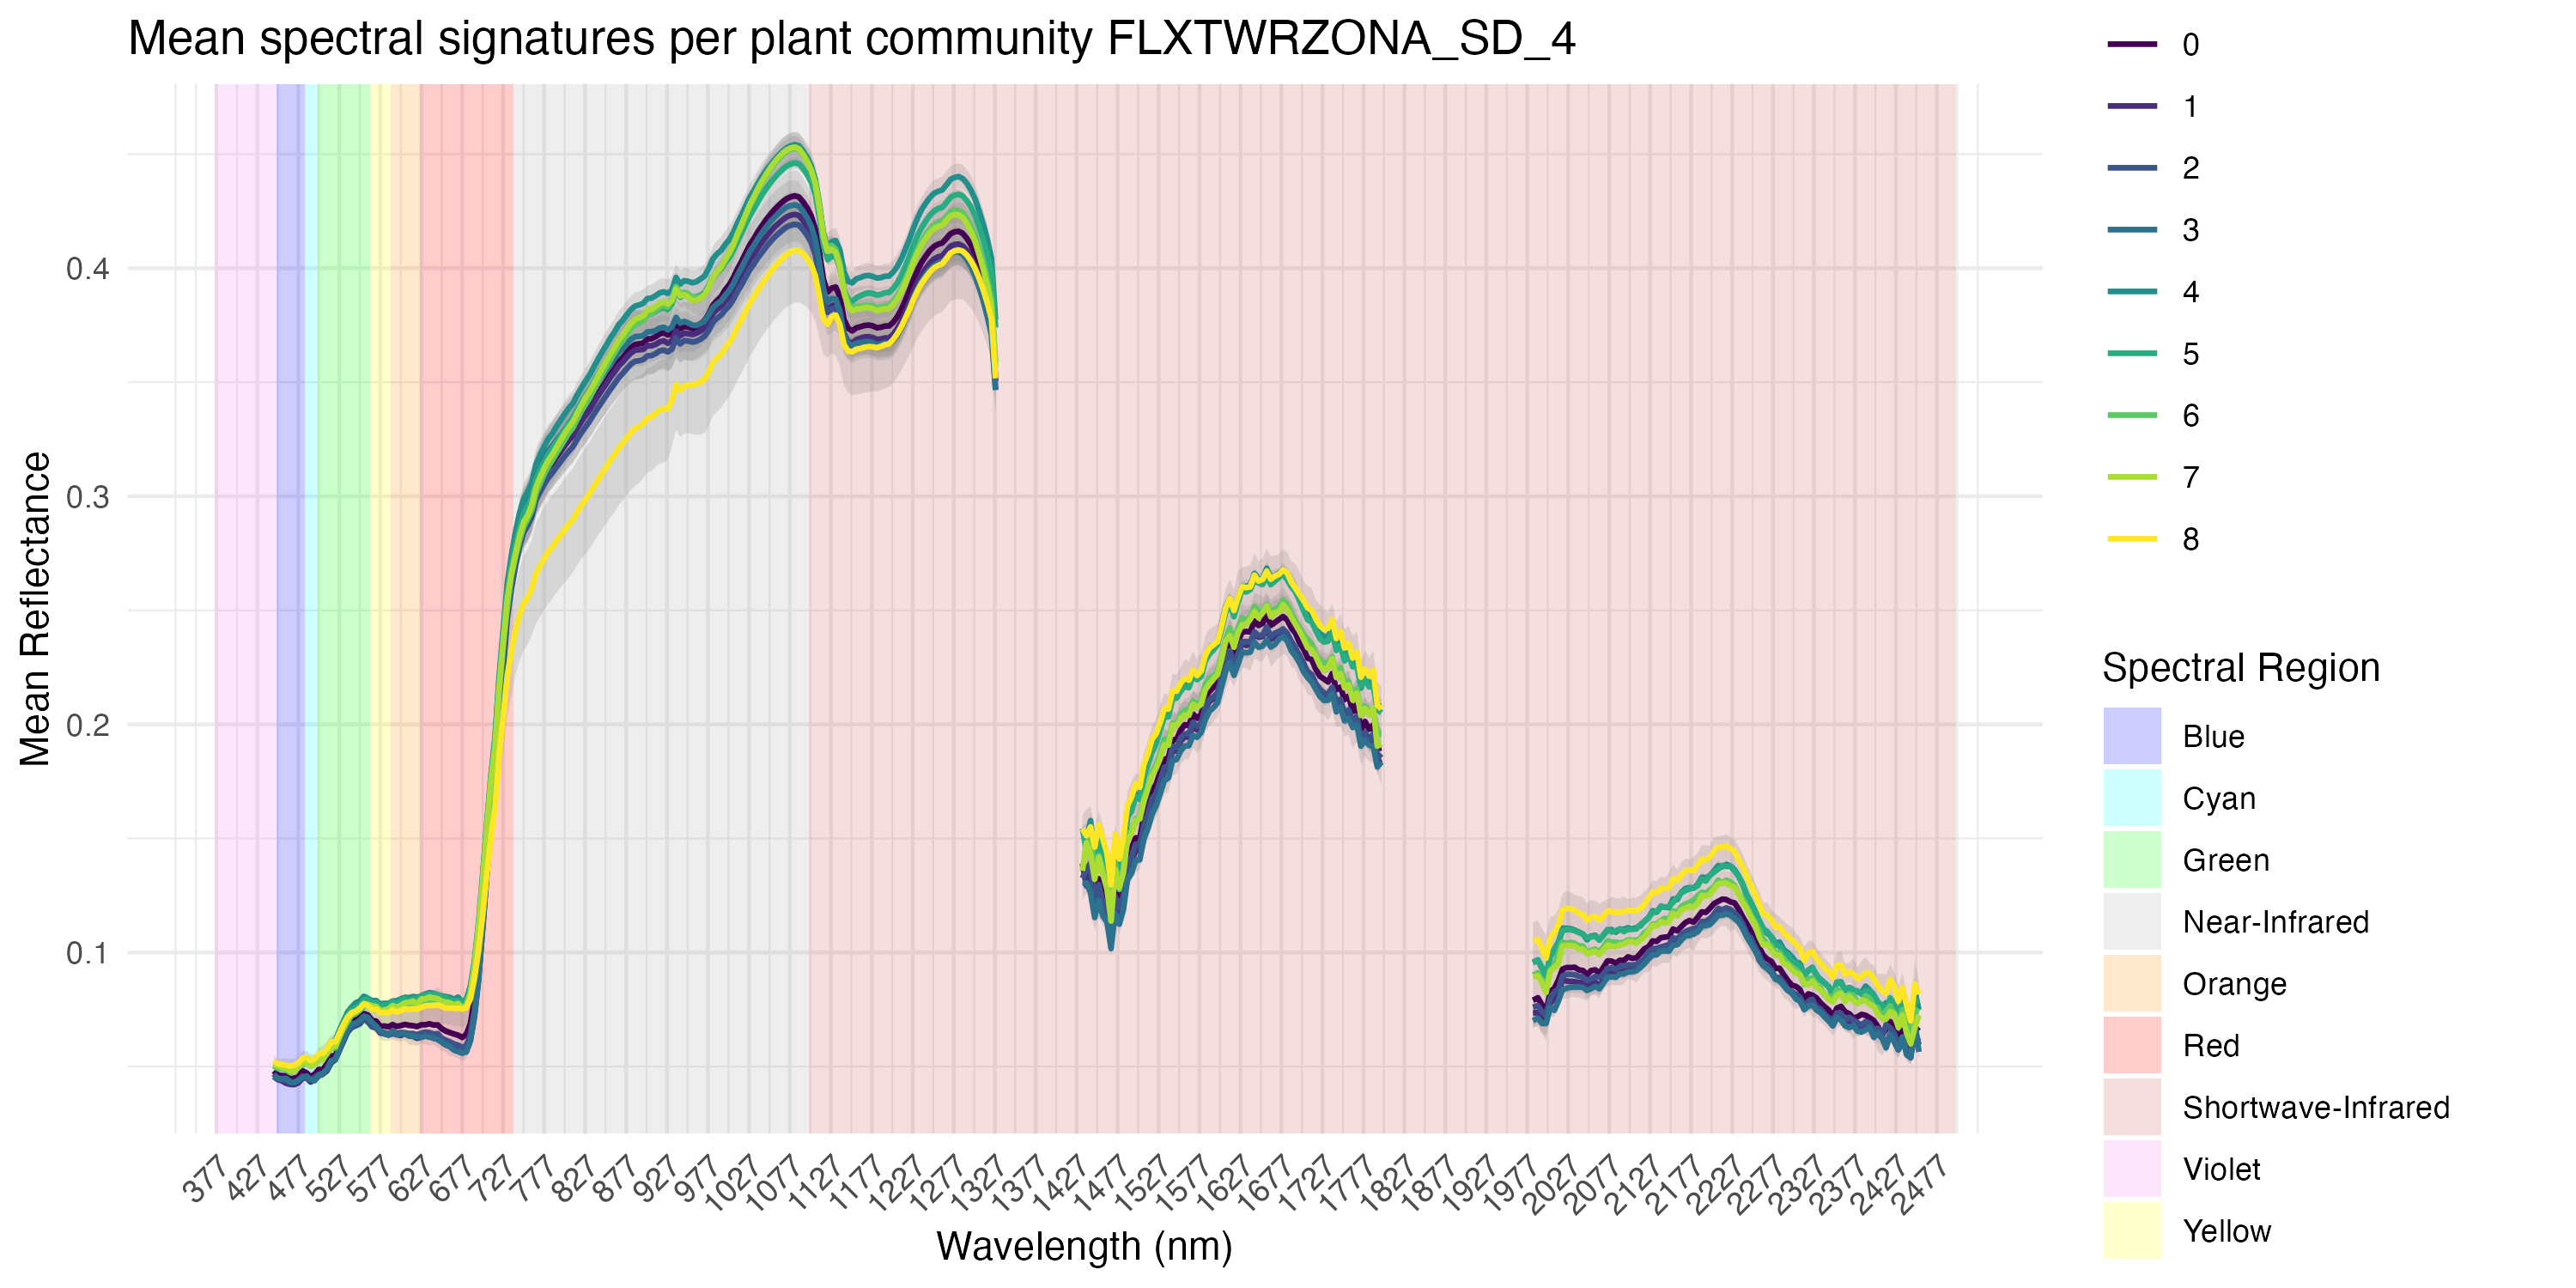
\includegraphics[width=\textwidth]{Figures/spectral_signatures/FLXTWRZONA_SD_4_mean_signature_plot_plant_community.png}
    \caption{}
    \label{fig:mss_pc_flxtwrzonasd4}
  \end{subfigure}

  \caption{Spectral signature plot \ref{fig:ss_pc_flxtwrzonasd4} and mean spectral signature plot \ref{fig:mss_pc_flxtwrzonasd4} grouped by plant community cluster for test site FLXTWRZONA\_SD\_4}
  \label{fig:group_pc_ht_flxtwrzonasd4}
\end{figure}

\subsection{FRST\_AK\_2}

\begin{figure}[H]
  \centering

  \begin{subfigure}[b]{0.49\textwidth}
    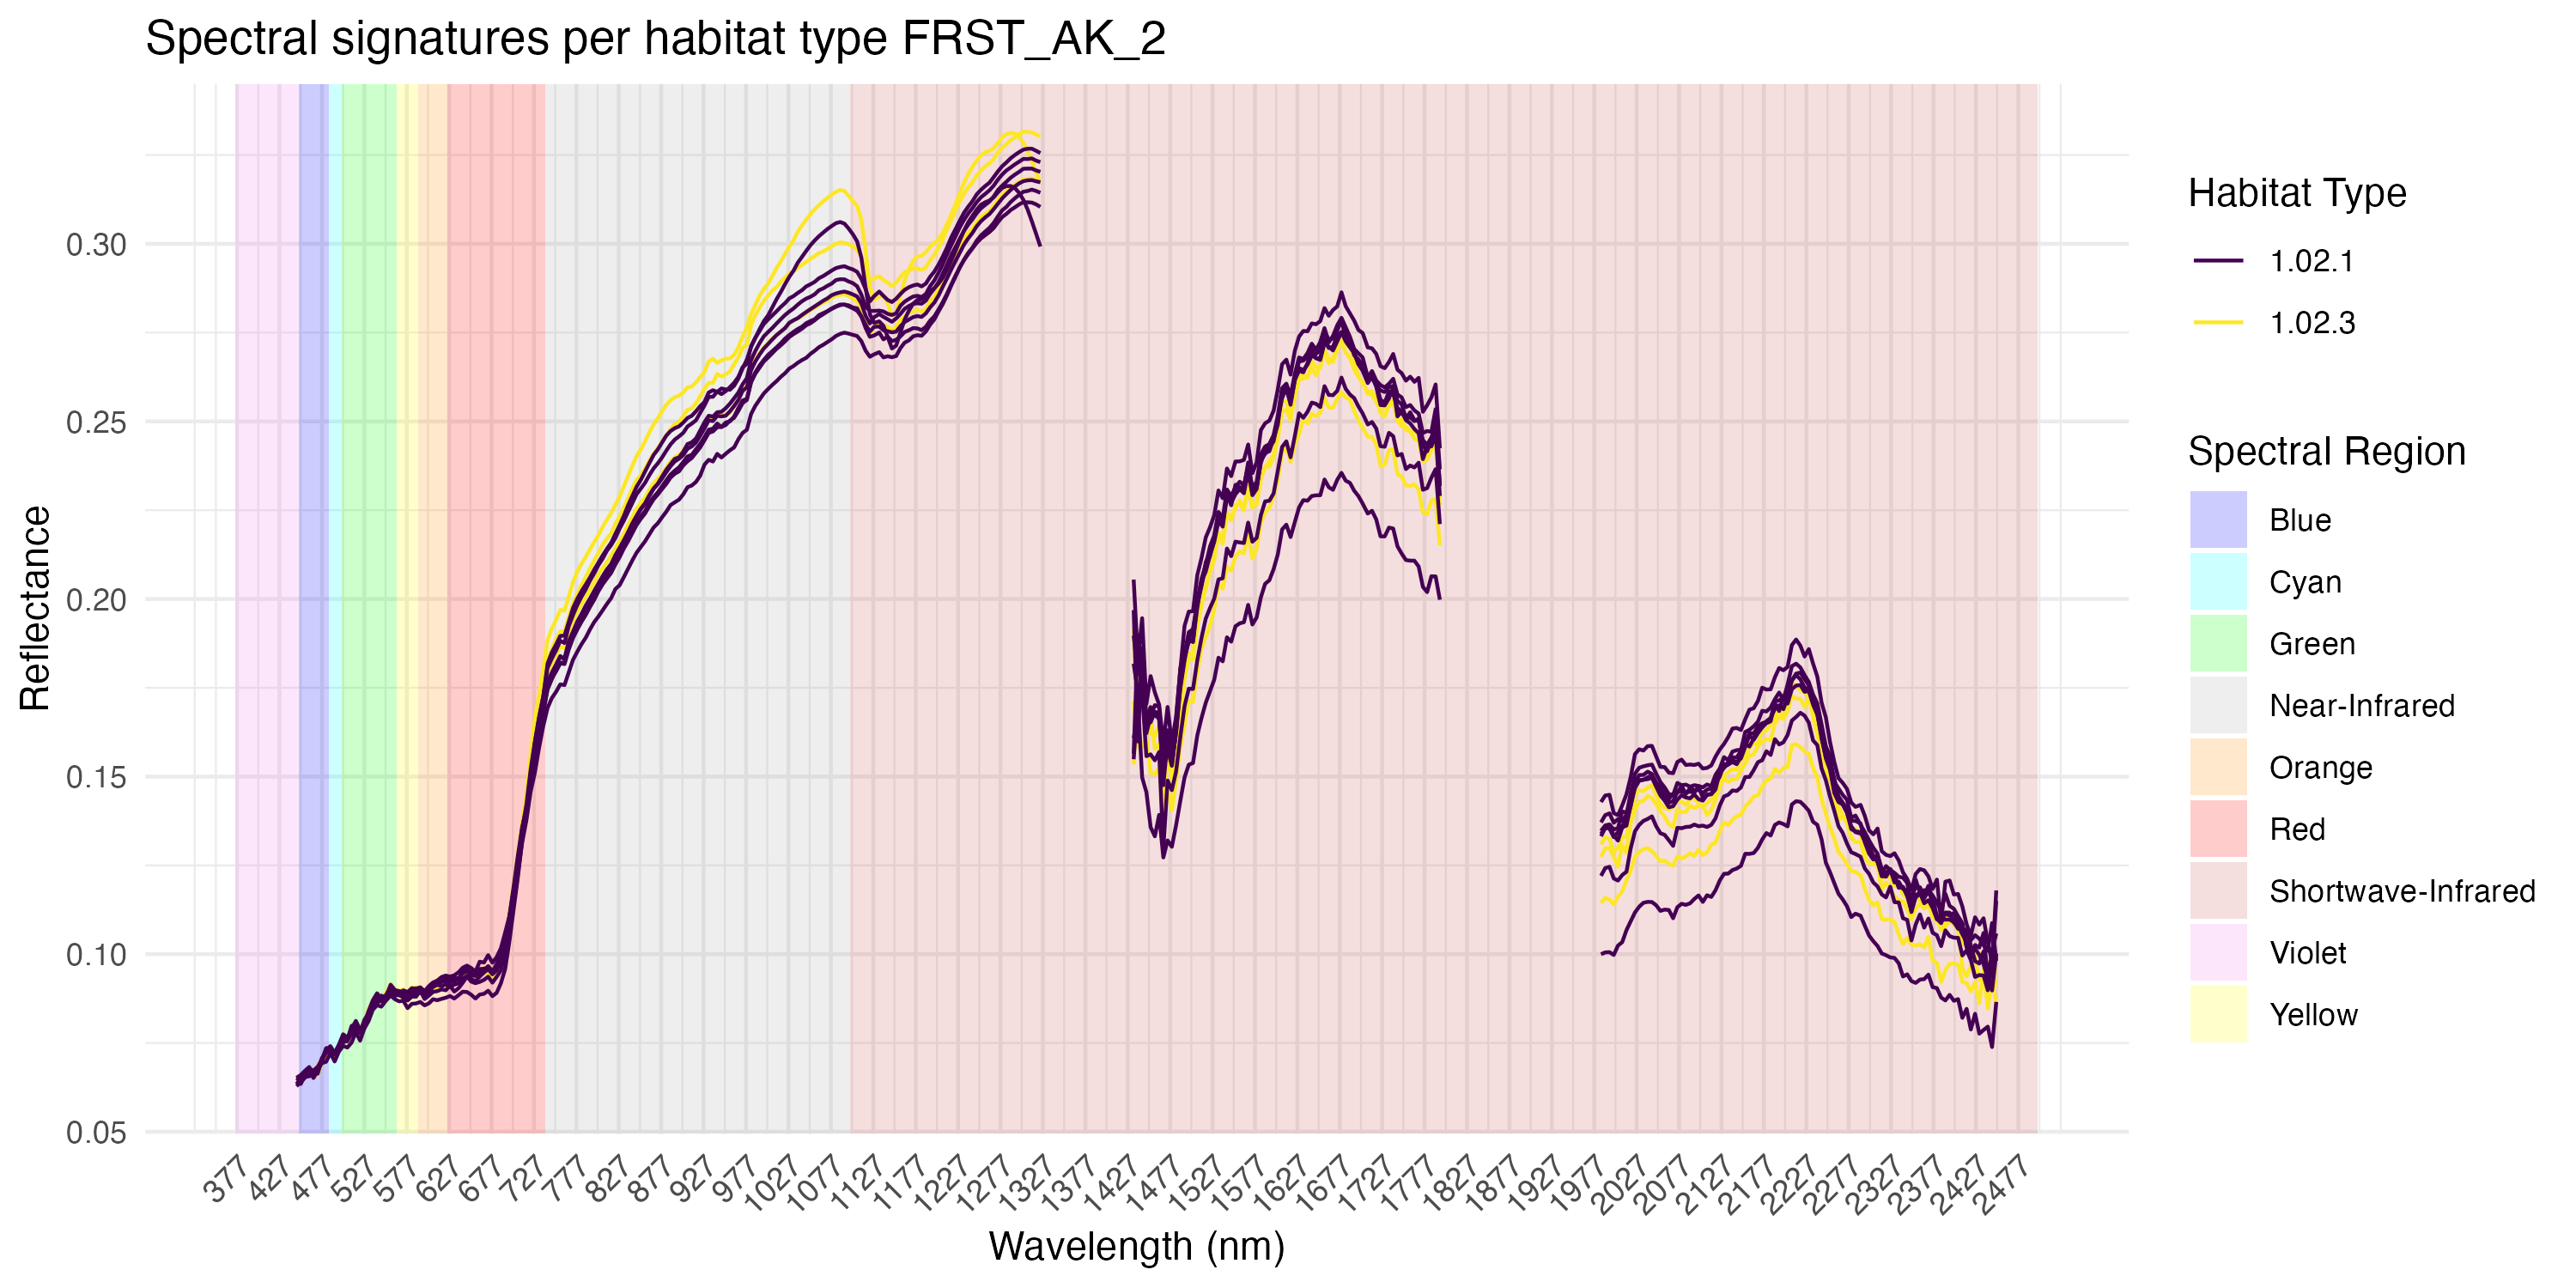
\includegraphics[width=\textwidth]{Figures/spectral_signatures/FRST_AK_2_signature_plot_habitat.png}
    \caption{}
    \label{fig:ss_ht_frstak2}
  \end{subfigure}
  \hfill
  \begin{subfigure}[b]{0.49\textwidth}
    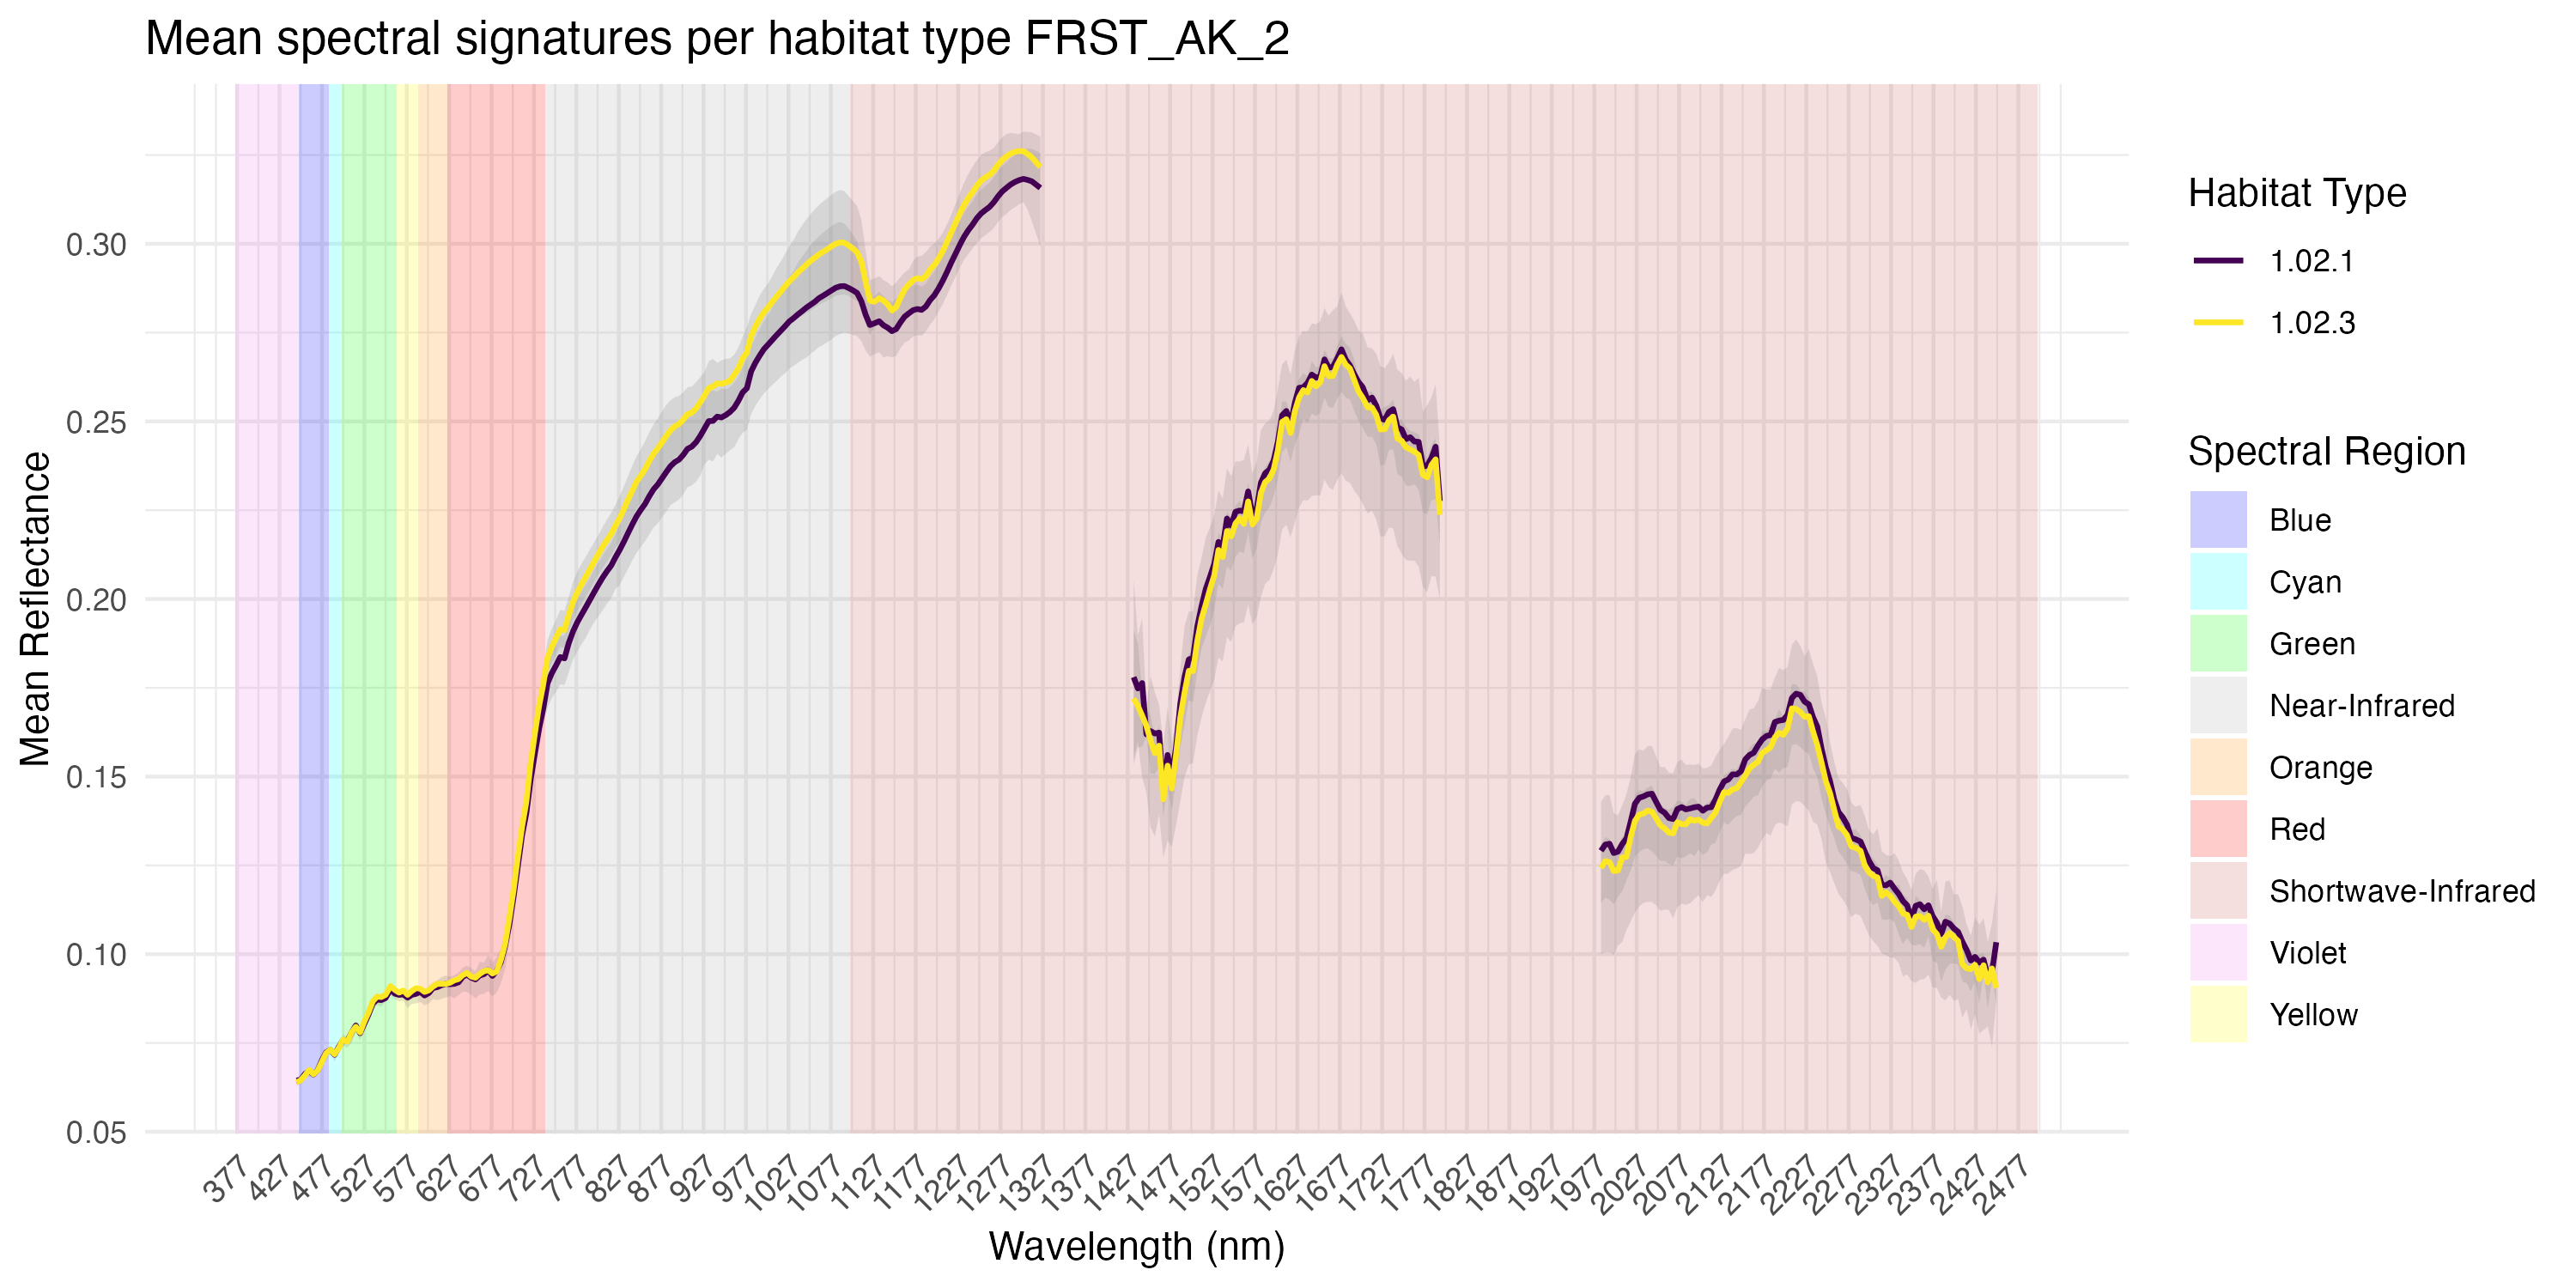
\includegraphics[width=\textwidth]{Figures/spectral_signatures/FRST_AK_2_mean_signature_plot_habitat.png}
    \caption{}
    \label{fig:mss_ht_frstak2}
  \end{subfigure}

  \caption{Spectral signature plot \ref{fig:ss_ht_frstak2} and mean spectral signature plot \ref{fig:mss_ht_frstak2} grouped by habitat type for test site FRST\_AK\_2}
  \label{fig:group_ss_ht_frstak2}
\end{figure}

\begin{figure}[H]
  \centering

  \begin{subfigure}[b]{0.49\textwidth}
    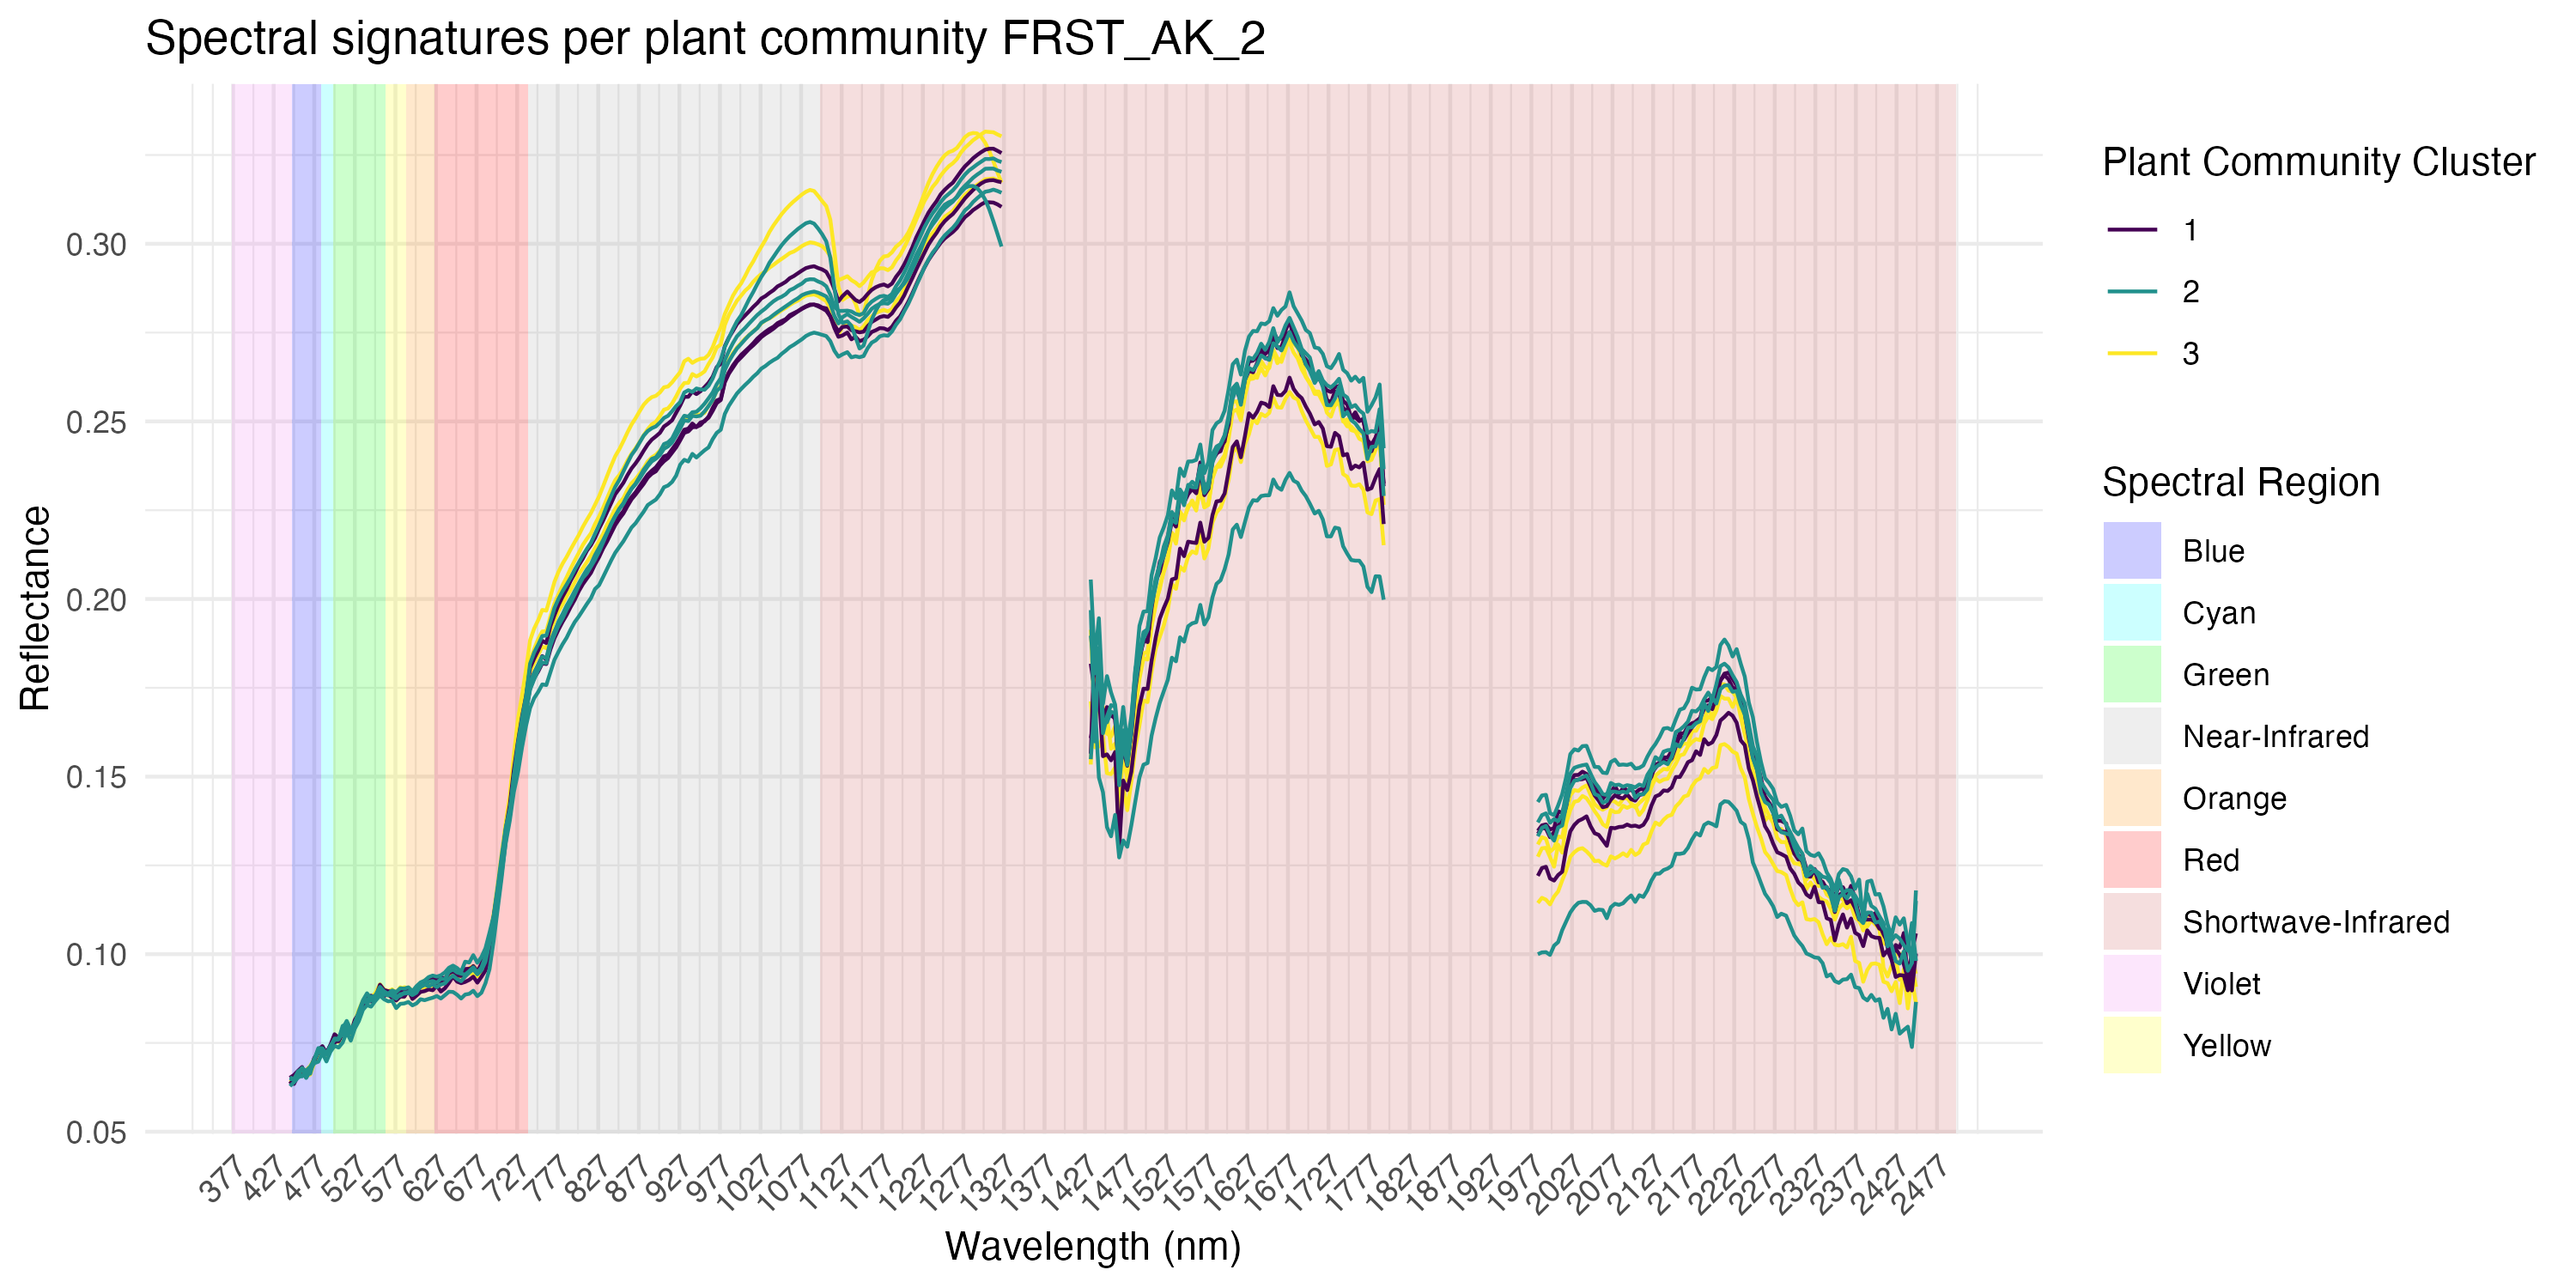
\includegraphics[width=\textwidth]{Figures/spectral_signatures/FRST_AK_2_signature_plot_plant_community.png}
    \caption{}
    \label{fig:ss_pc_frstak2}
  \end{subfigure}
  \hfill
  \begin{subfigure}[b]{0.49\textwidth}
    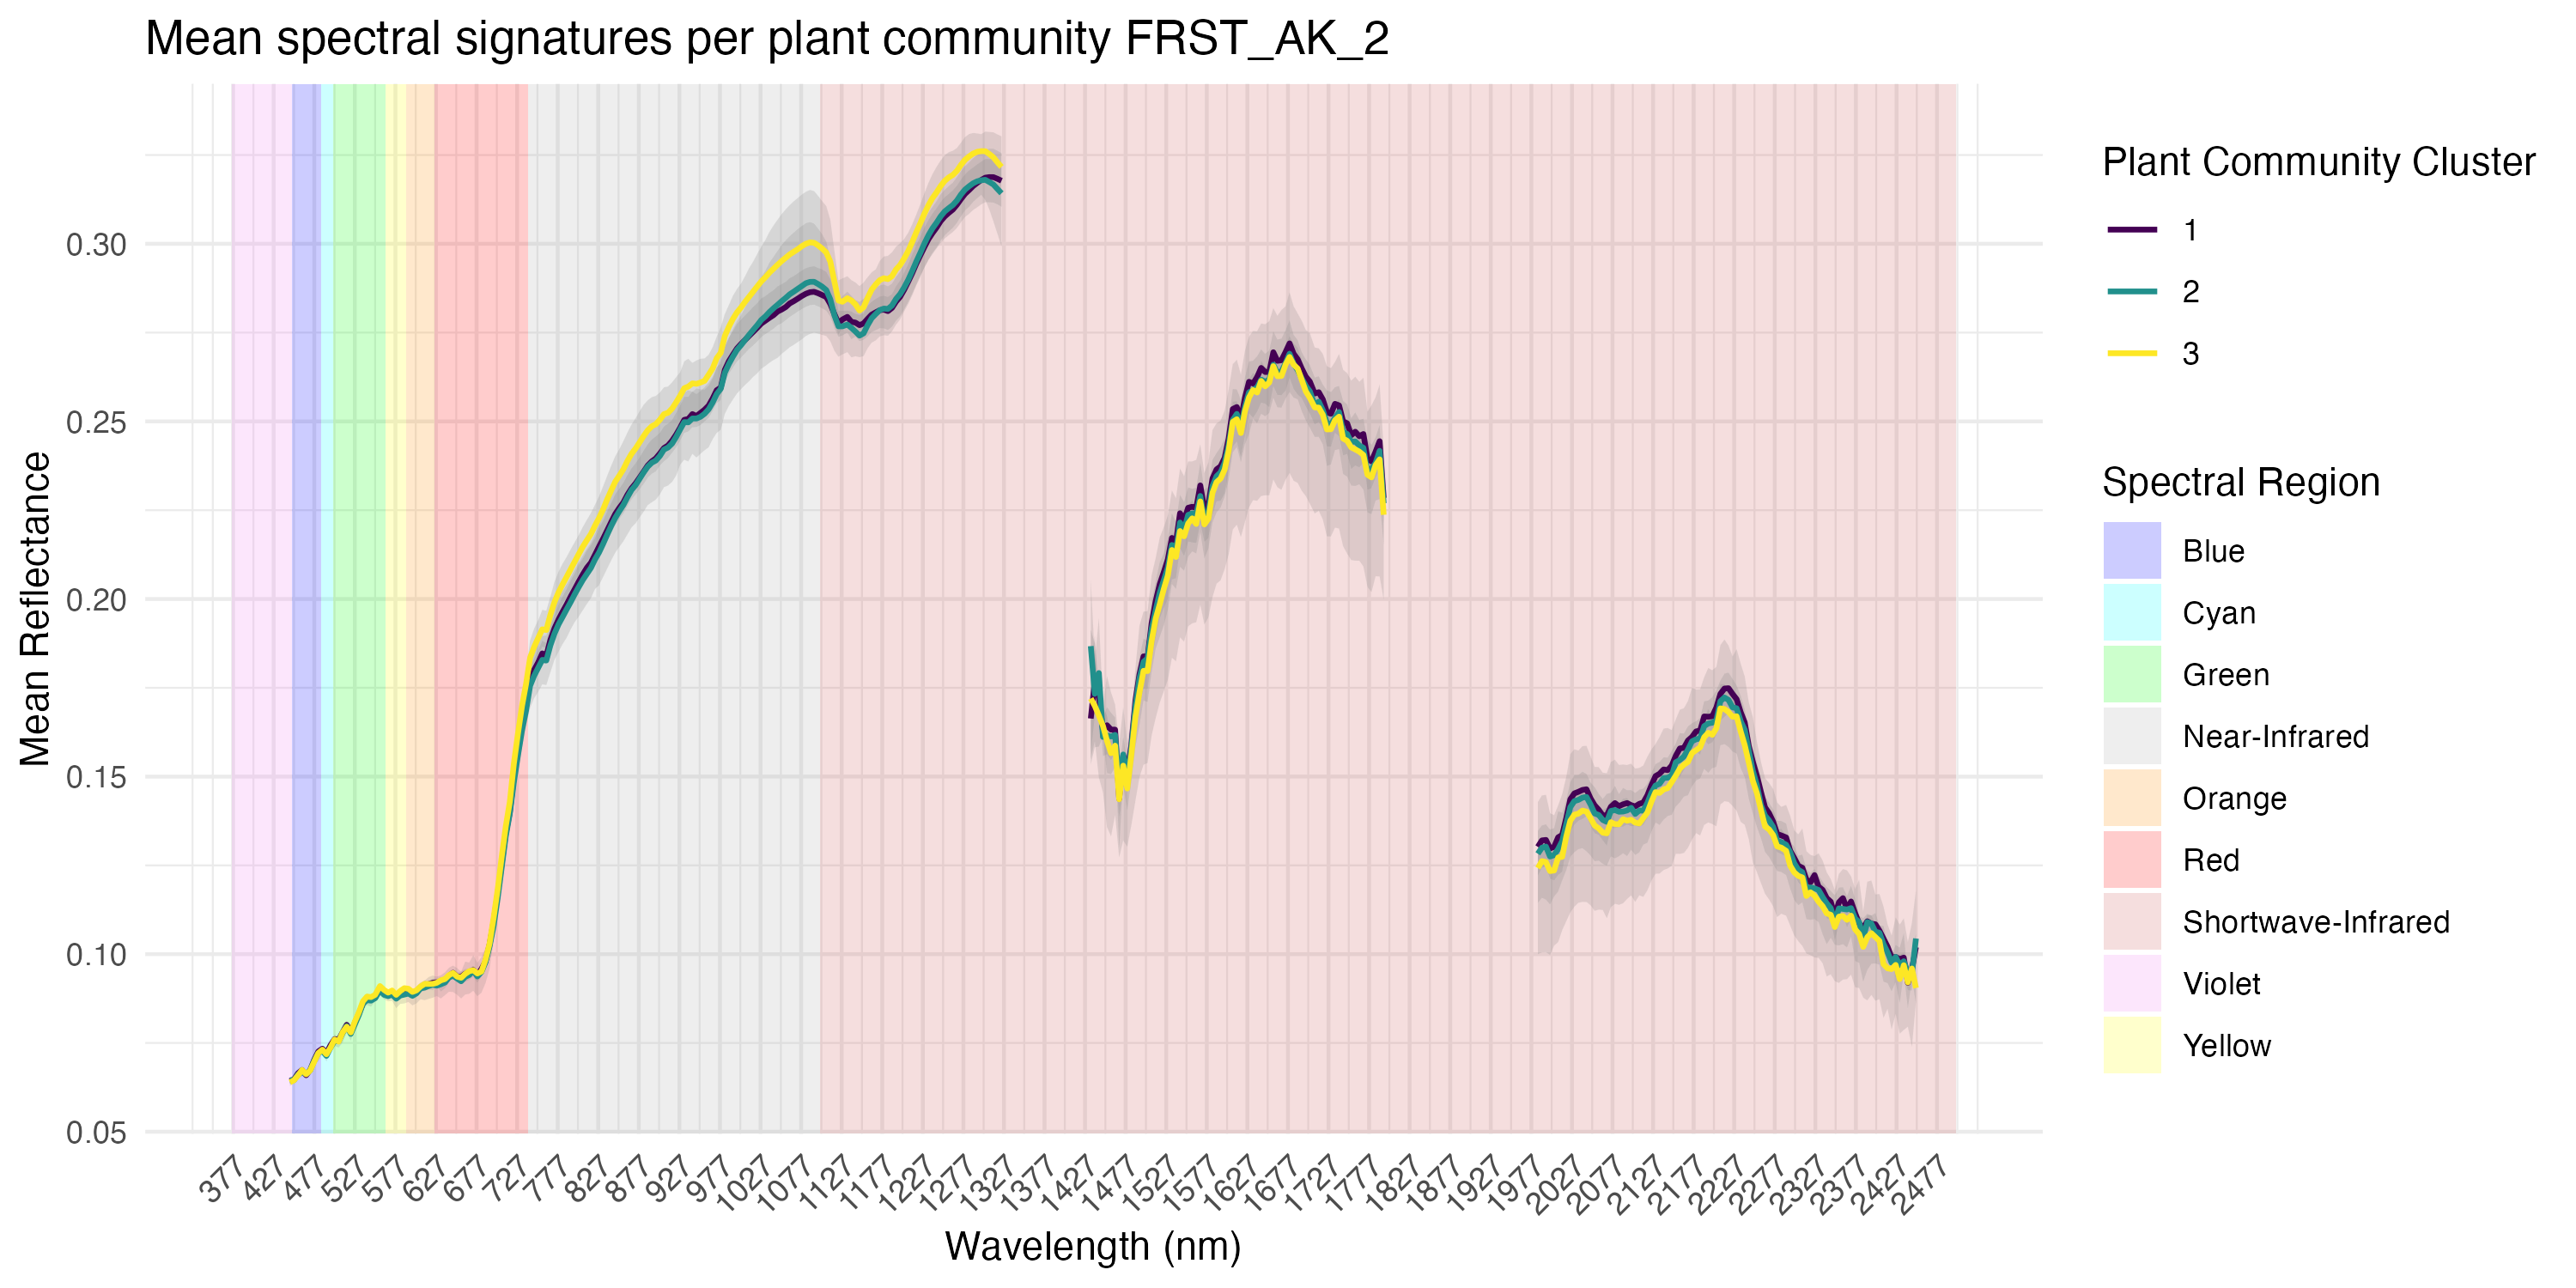
\includegraphics[width=\textwidth]{Figures/spectral_signatures/FRST_AK_2_mean_signature_plot_plant_community.png}
    \caption{}
    \label{fig:mss_pc_frstak2}
  \end{subfigure}

  \caption{Spectral signature plot \ref{fig:ss_pc_frstak2} and mean spectral signature plot \ref{fig:mss_pc_frstak2} grouped by plant community cluster for test site FRST\_AK\_2}
  \label{fig:group_pc_ht_frstak2}
\end{figure}

\subsection{FRST\_AK\_3}

\begin{figure}[H]
  \centering

  \begin{subfigure}[b]{0.49\textwidth}
    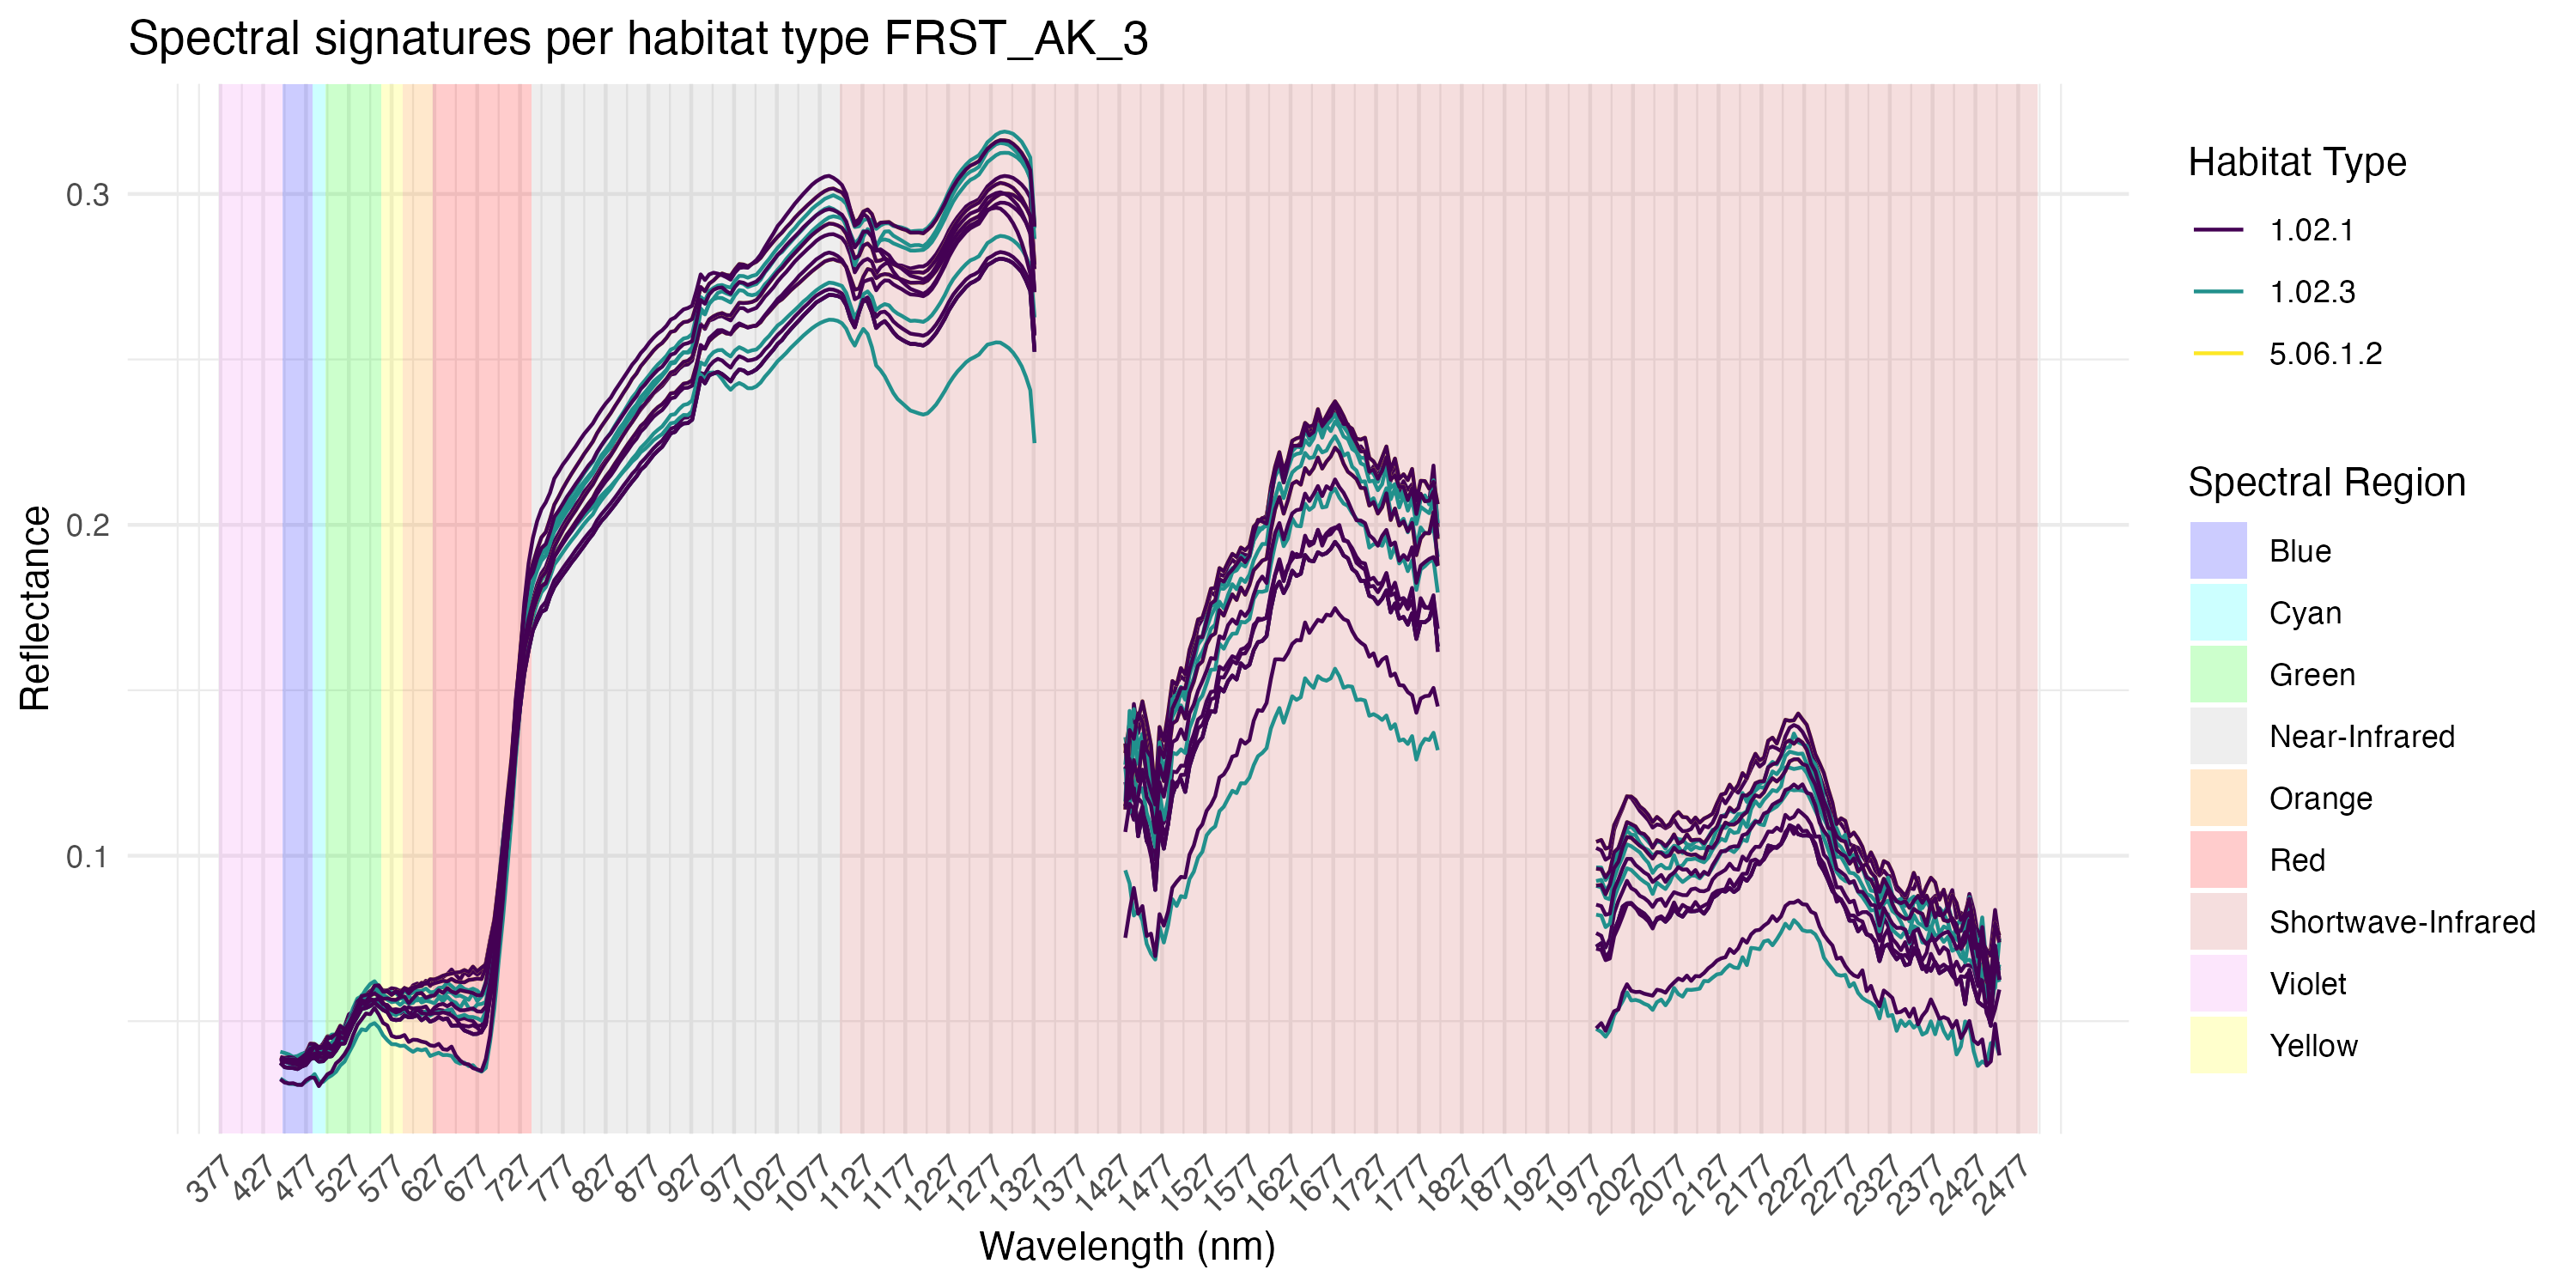
\includegraphics[width=\textwidth]{Figures/spectral_signatures/FRST_AK_3_signature_plot_habitat.png}
    \caption{}
    \label{fig:ss_ht_frstak3}
  \end{subfigure}
  \hfill
  \begin{subfigure}[b]{0.49\textwidth}
    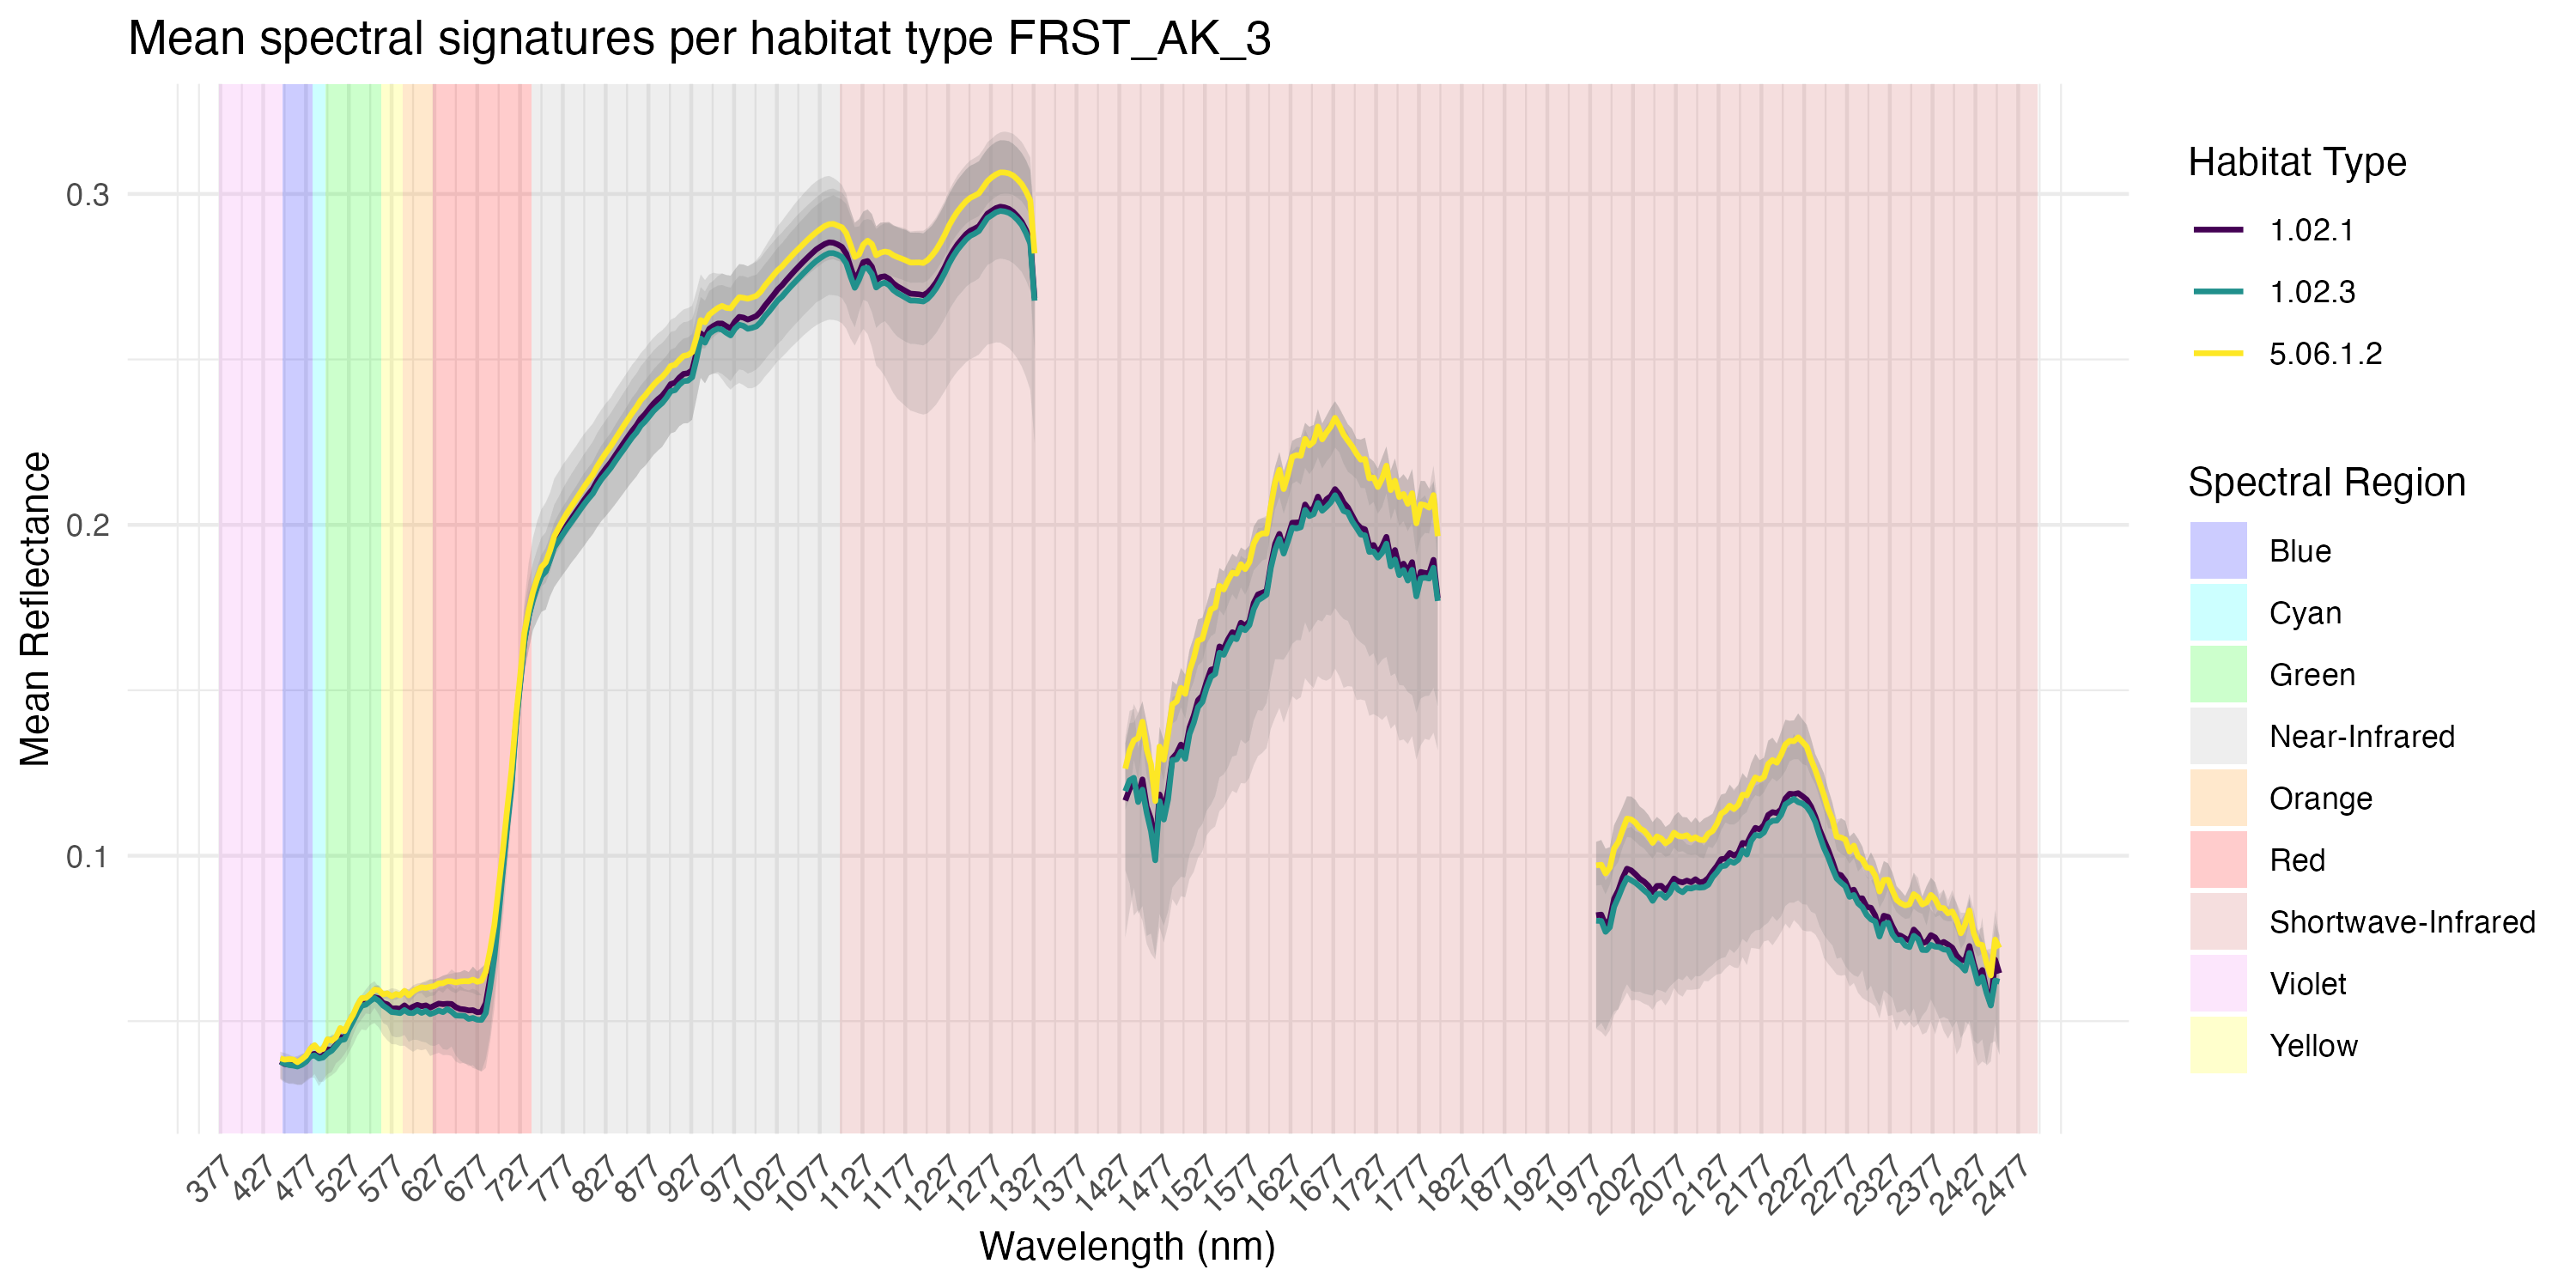
\includegraphics[width=\textwidth]{Figures/spectral_signatures/FRST_AK_3_mean_signature_plot_habitat.png}
    \caption{}
    \label{fig:mss_ht_frstak3}
  \end{subfigure}

  \caption{Spectral signature plot \ref{fig:ss_ht_frstak3} and mean spectral signature plot \ref{fig:mss_ht_frstak3} grouped by habitat type for test site FRST\_AK\_3}
  \label{fig:group_ss_ht_frstak3}
\end{figure}

\begin{figure}[H]
  \centering

  \begin{subfigure}[b]{0.49\textwidth}
    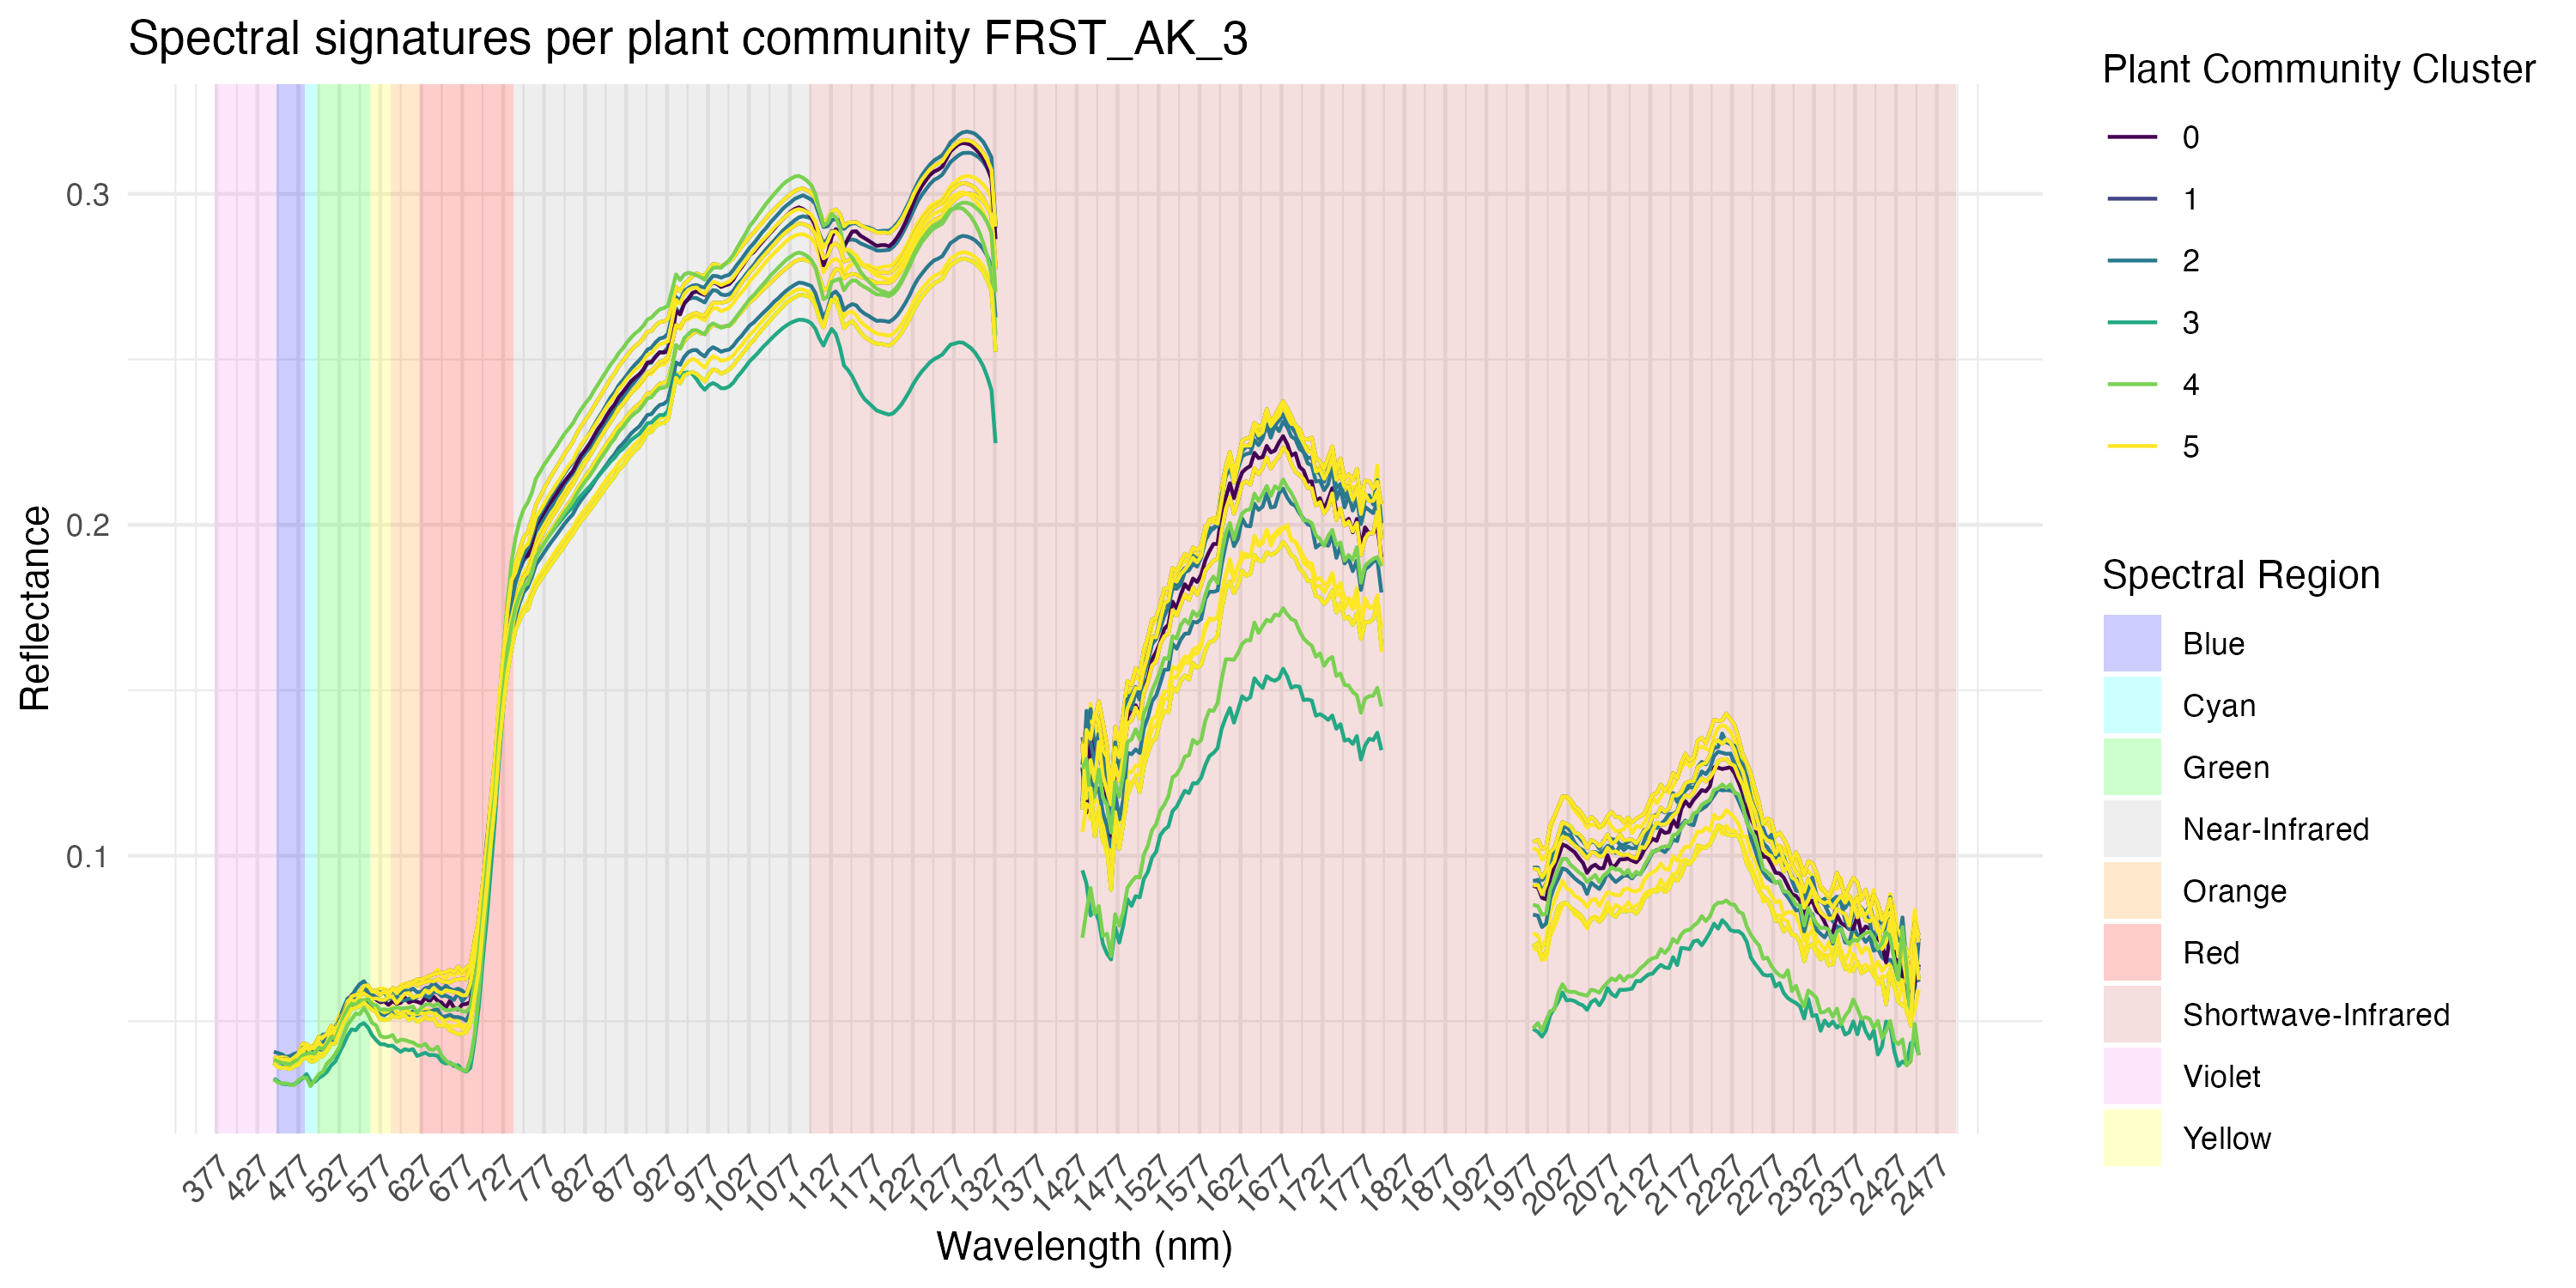
\includegraphics[width=\textwidth]{Figures/spectral_signatures/FRST_AK_3_signature_plot_plant_community.png}
    \caption{}
    \label{fig:ss_pc_frstak3}
  \end{subfigure}
  \hfill
  \begin{subfigure}[b]{0.49\textwidth}
    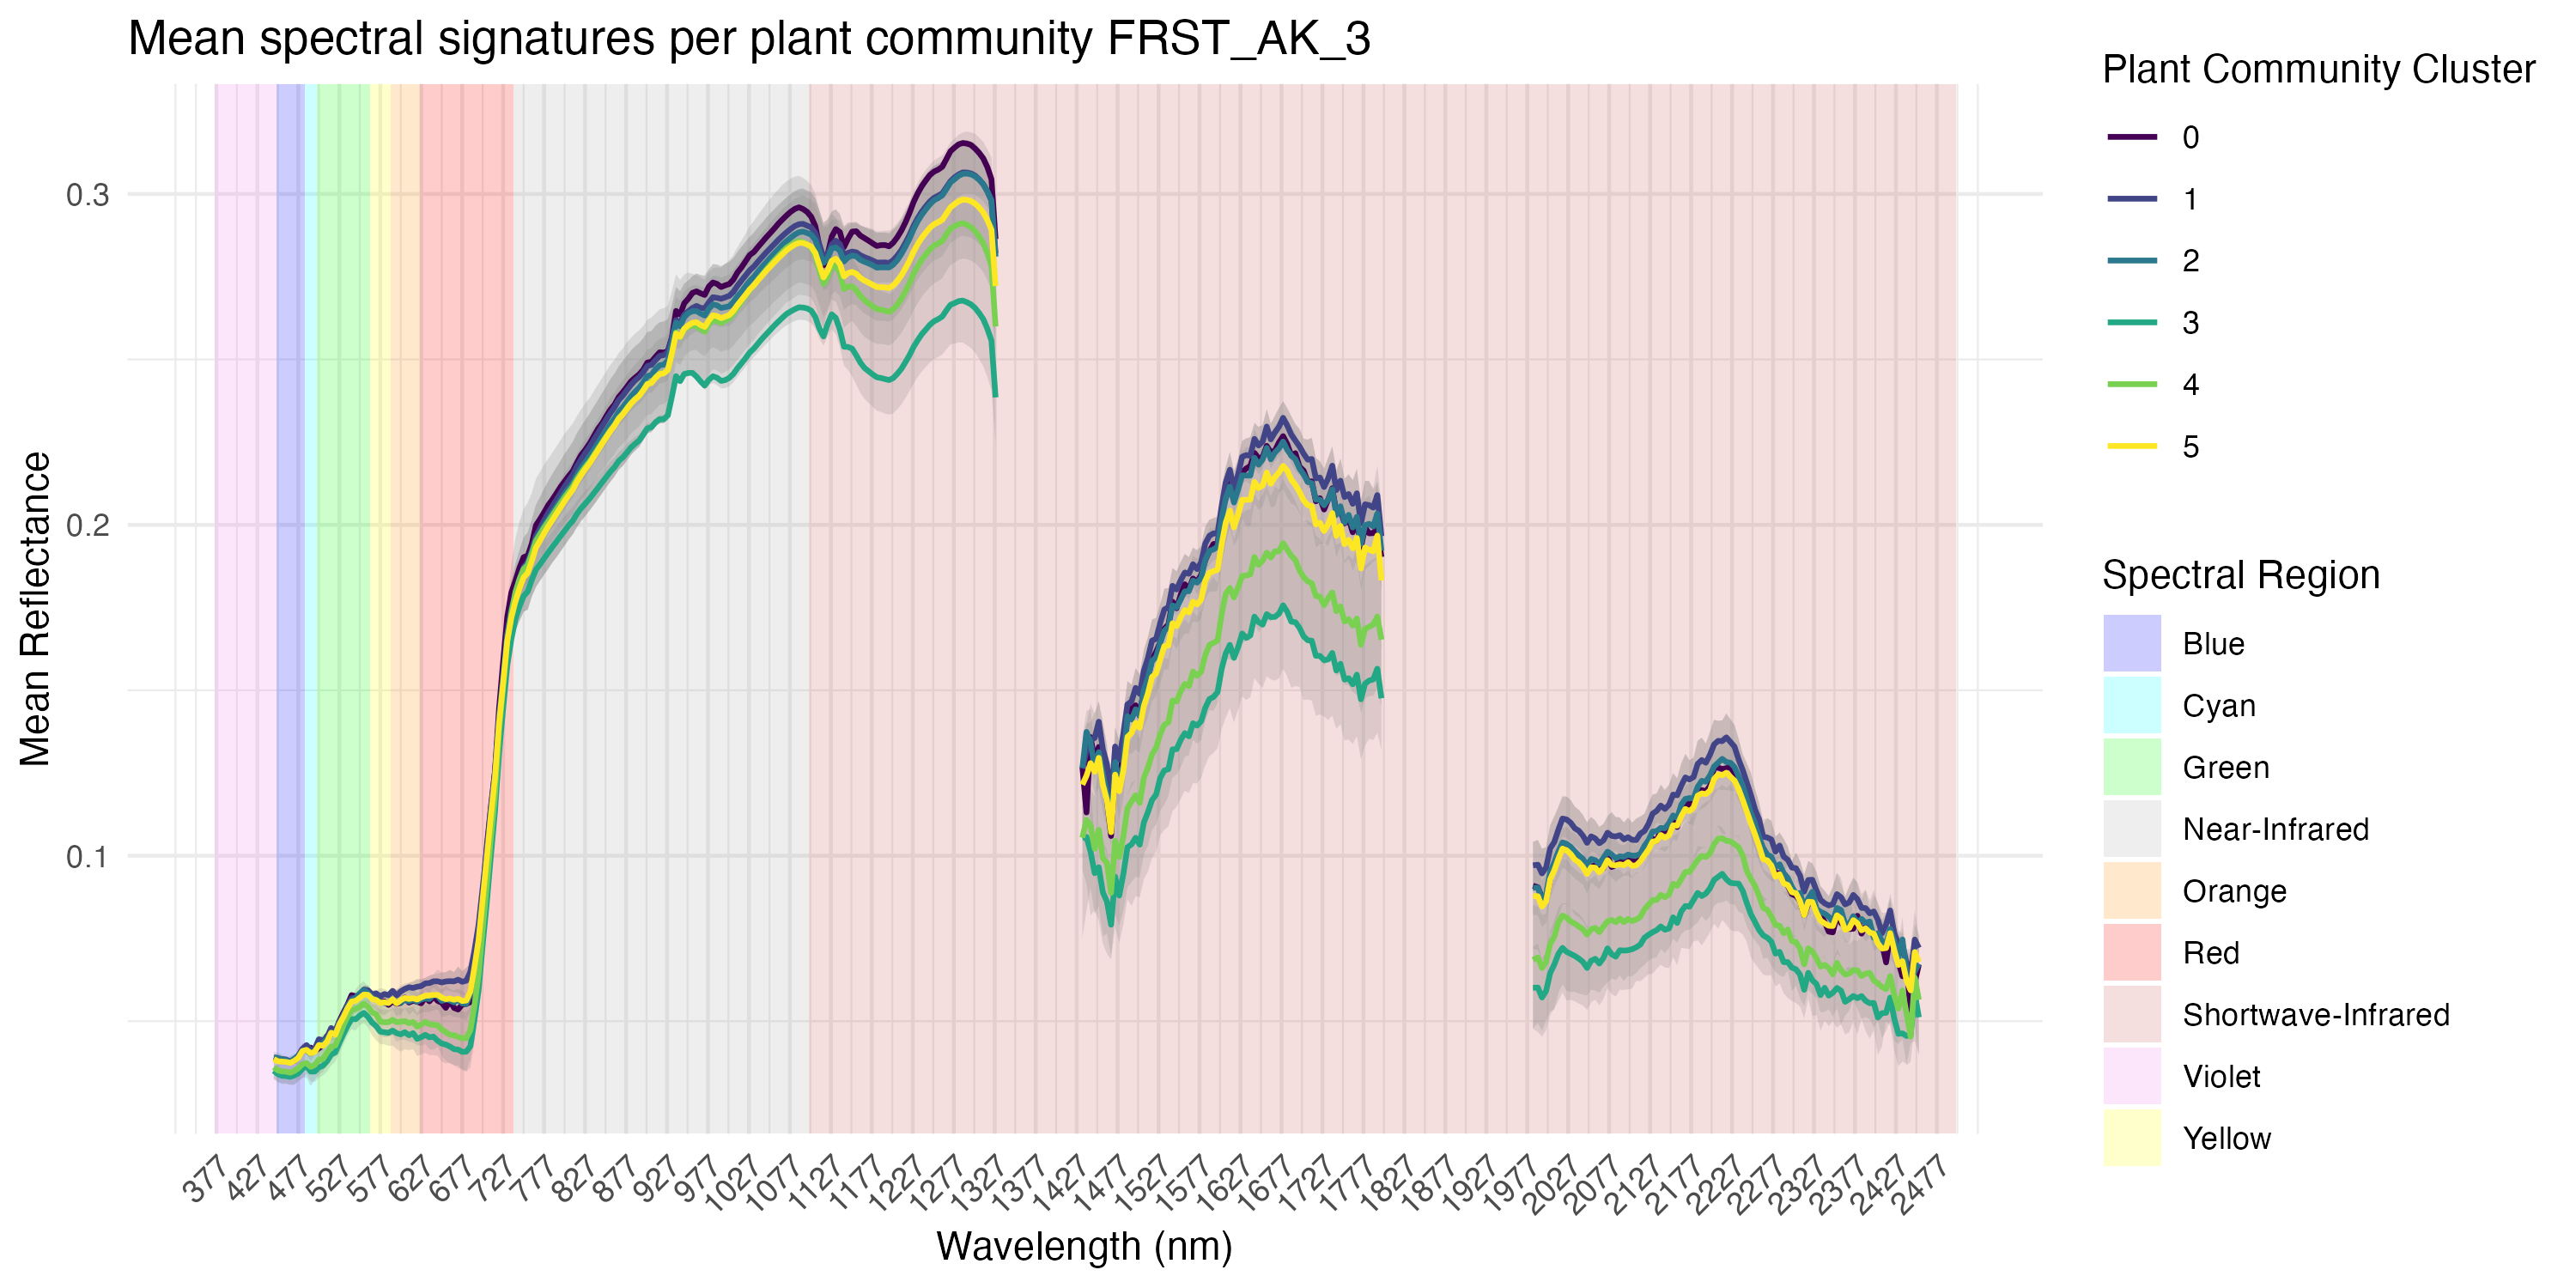
\includegraphics[width=\textwidth]{Figures/spectral_signatures/FRST_AK_3_mean_signature_plot_plant_community.png}
    \caption{}
    \label{fig:mss_pc_frstak3}
  \end{subfigure}

  \caption{Spectral signature plot \ref{fig:ss_pc_frstak3} and mean spectral signature plot \ref{fig:mss_pc_frstak3} grouped by plant community cluster for test site FRST\_AK\_3}
  \label{fig:group_pc_ht_frstak3}
\end{figure}

\subsection{PRUAIR\_DW\_1}

\begin{figure}[H]
  \centering

  \begin{subfigure}[b]{0.49\textwidth}
    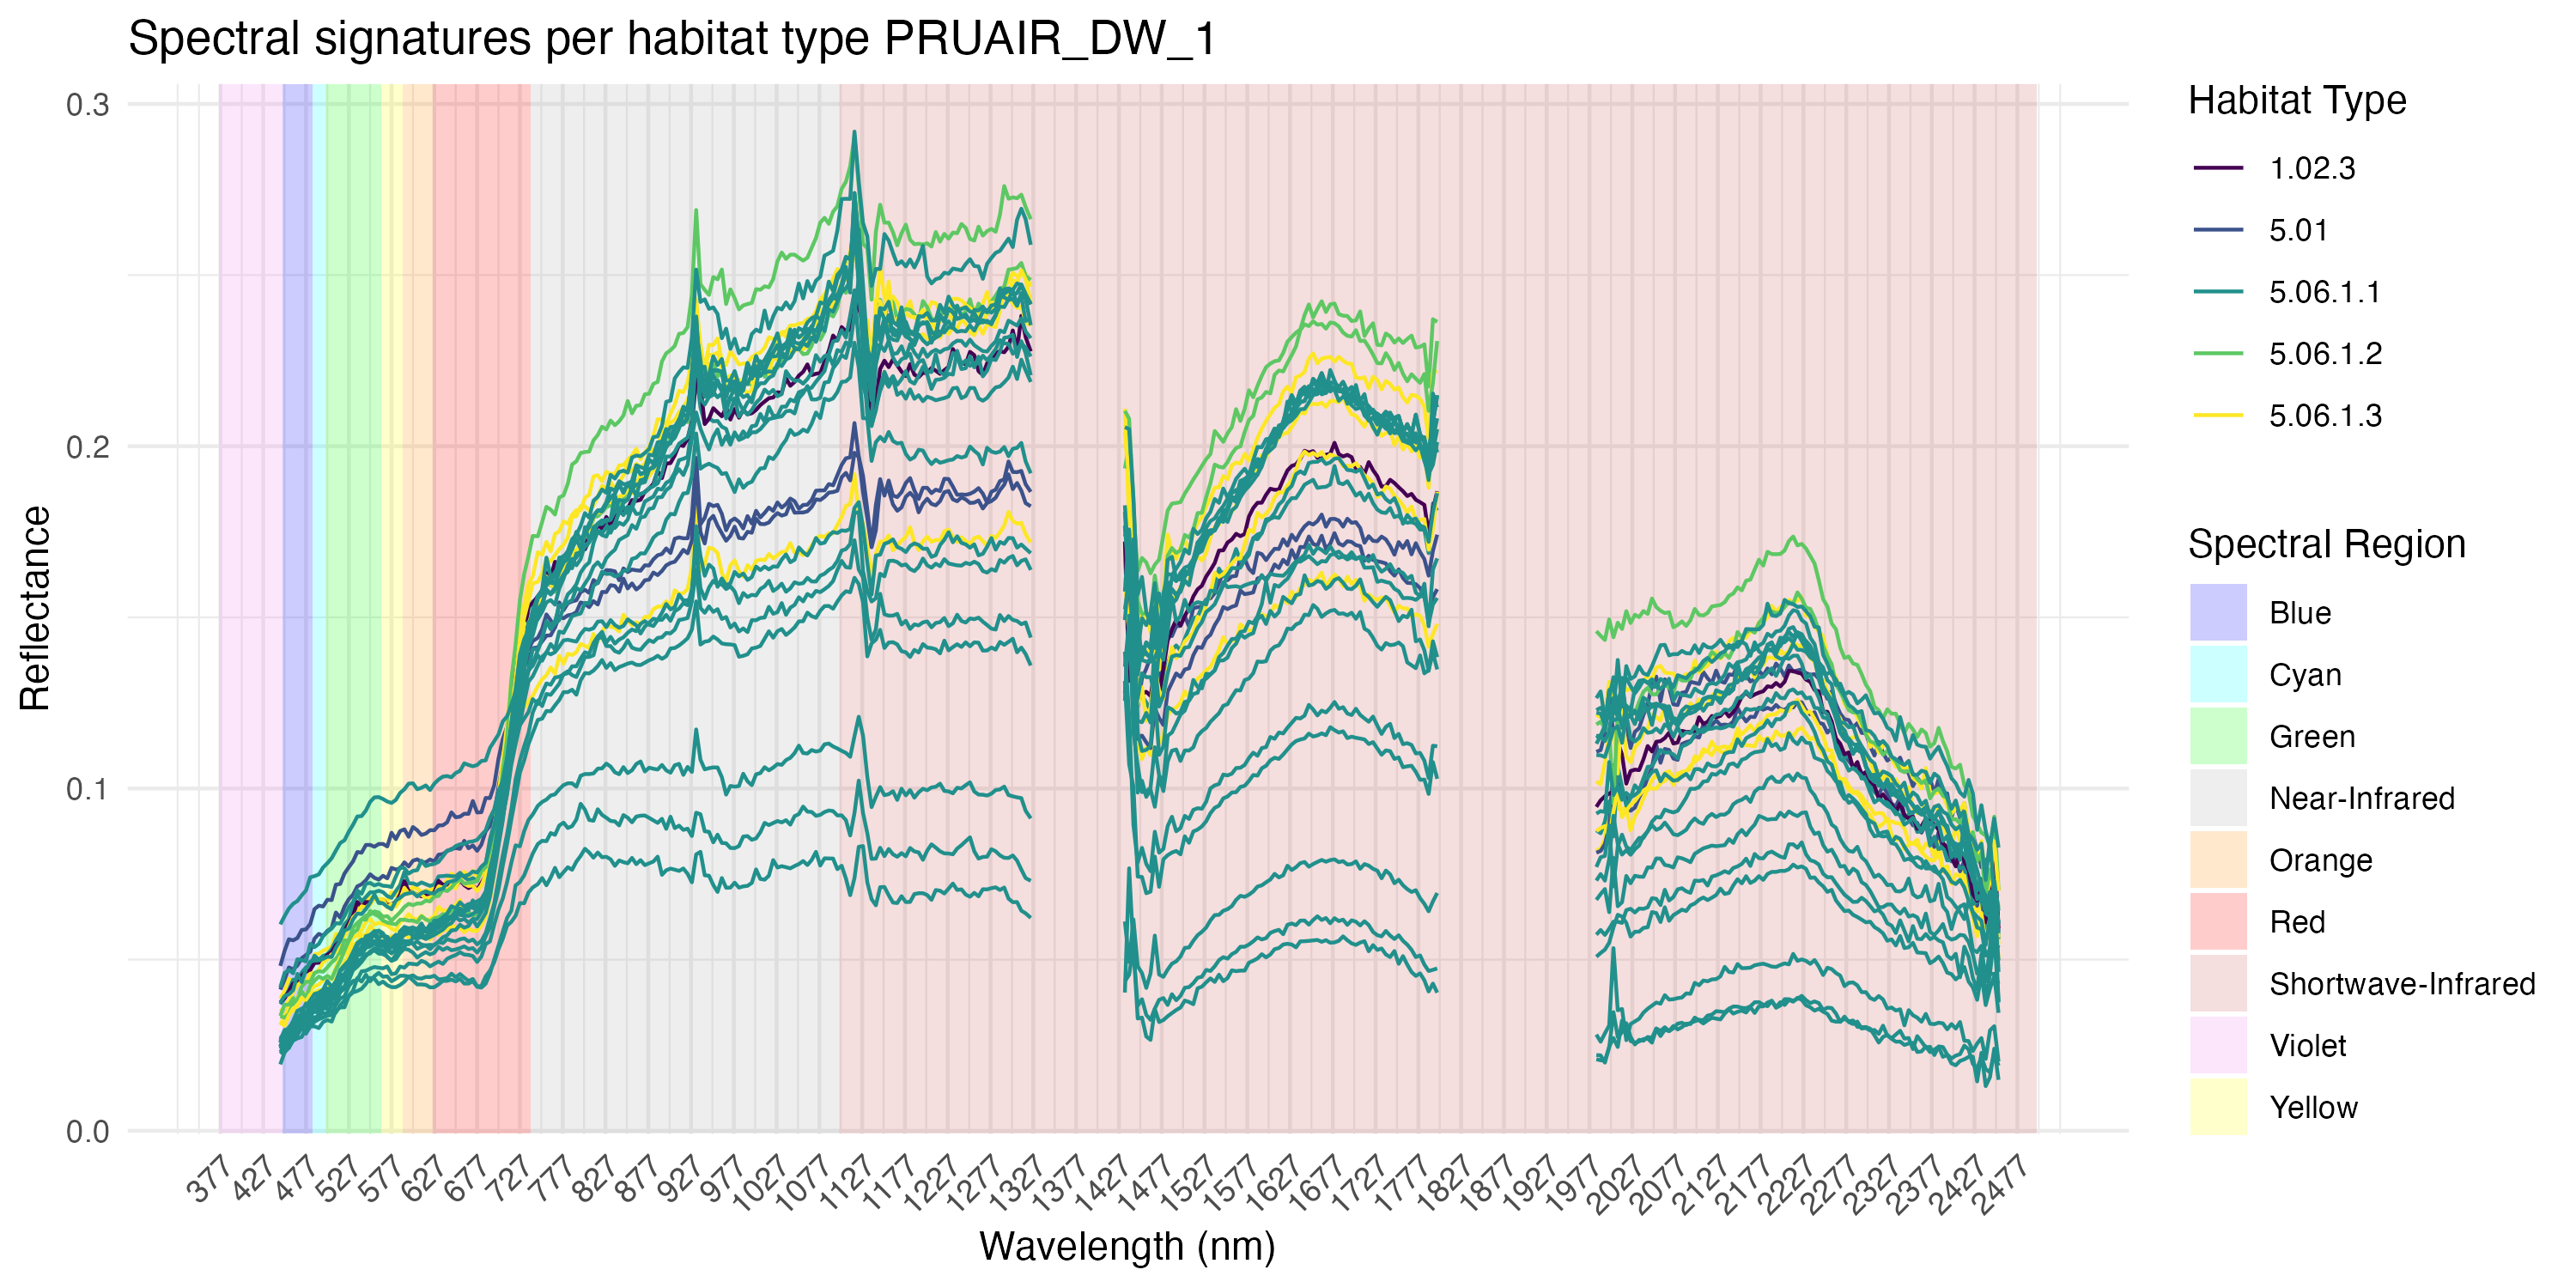
\includegraphics[width=\textwidth]{Figures/spectral_signatures/PRUAIR_DW_1_signature_plot_habitat.png}
    \caption{}
    \label{fig:ss_ht_pruairdw1}
  \end{subfigure}
  \hfill
  \begin{subfigure}[b]{0.49\textwidth}
    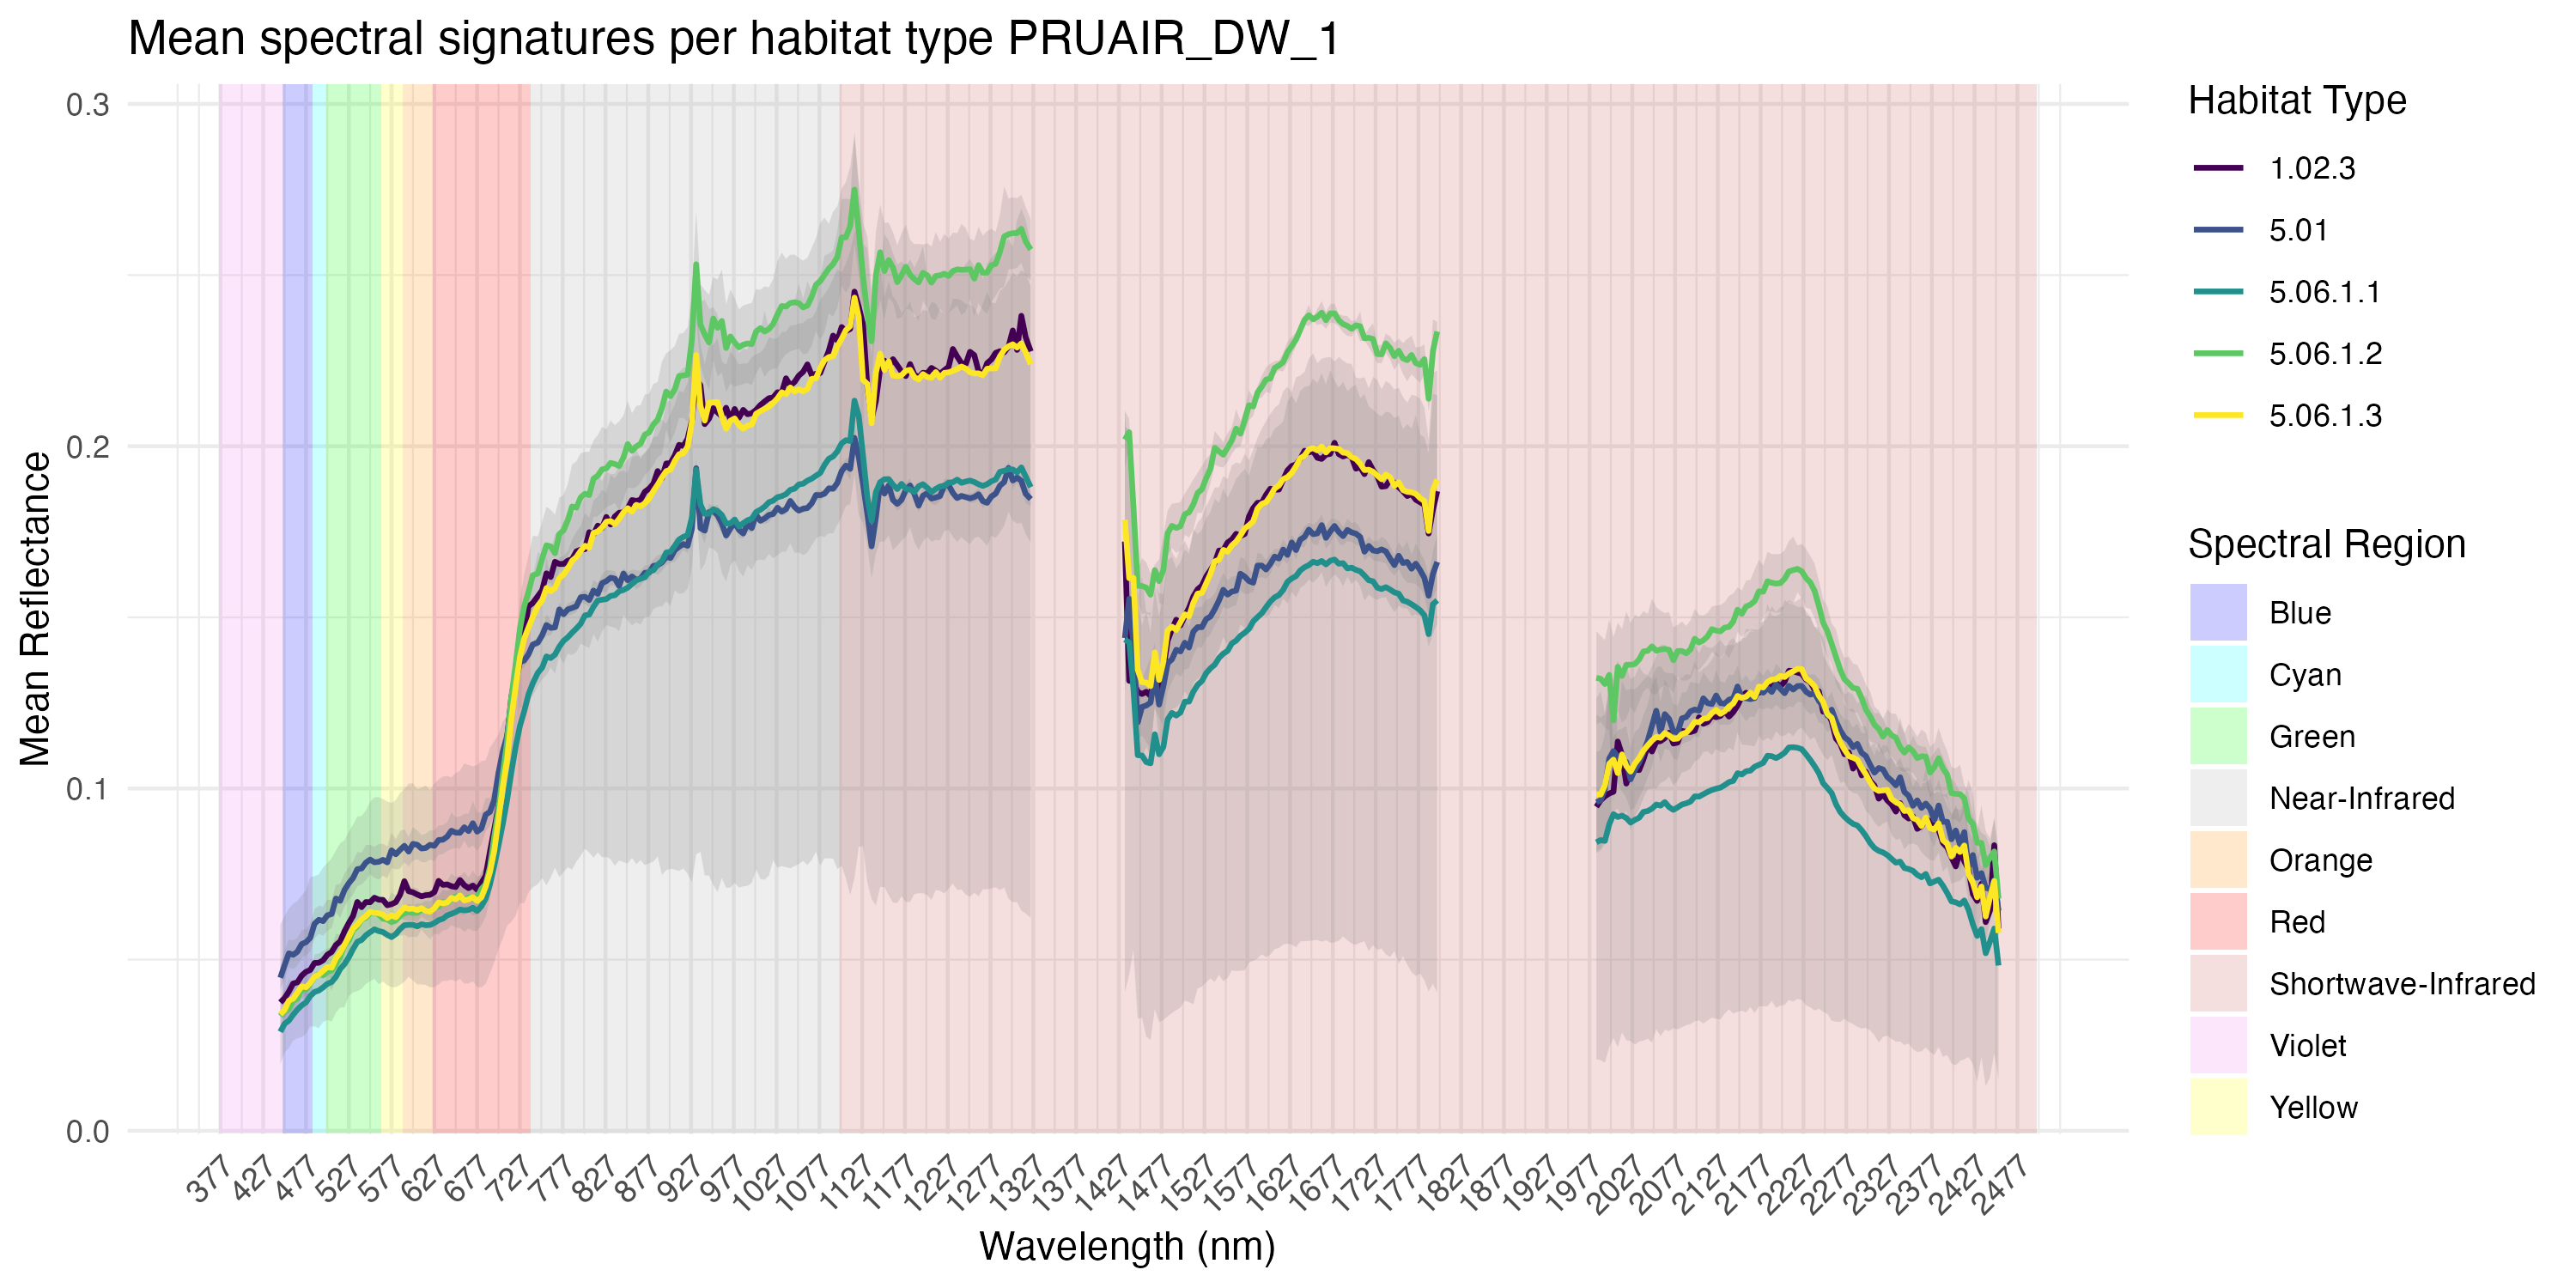
\includegraphics[width=\textwidth]{Figures/spectral_signatures/PRUAIR_DW_1_mean_signature_plot_habitat.png}
    \caption{}
    \label{fig:mss_ht_pruairdw1}
  \end{subfigure}

  \caption{Spectral signature plot \ref{fig:ss_ht_pruairdw1} and mean spectral signature plot \ref{fig:mss_ht_pruairdw1} grouped by habitat type for test site PRUAIR\_DW\_1}
  \label{fig:group_ss_ht_pruairdw1}
\end{figure}

\begin{figure}[H]
  \centering

  \begin{subfigure}[b]{0.49\textwidth}
    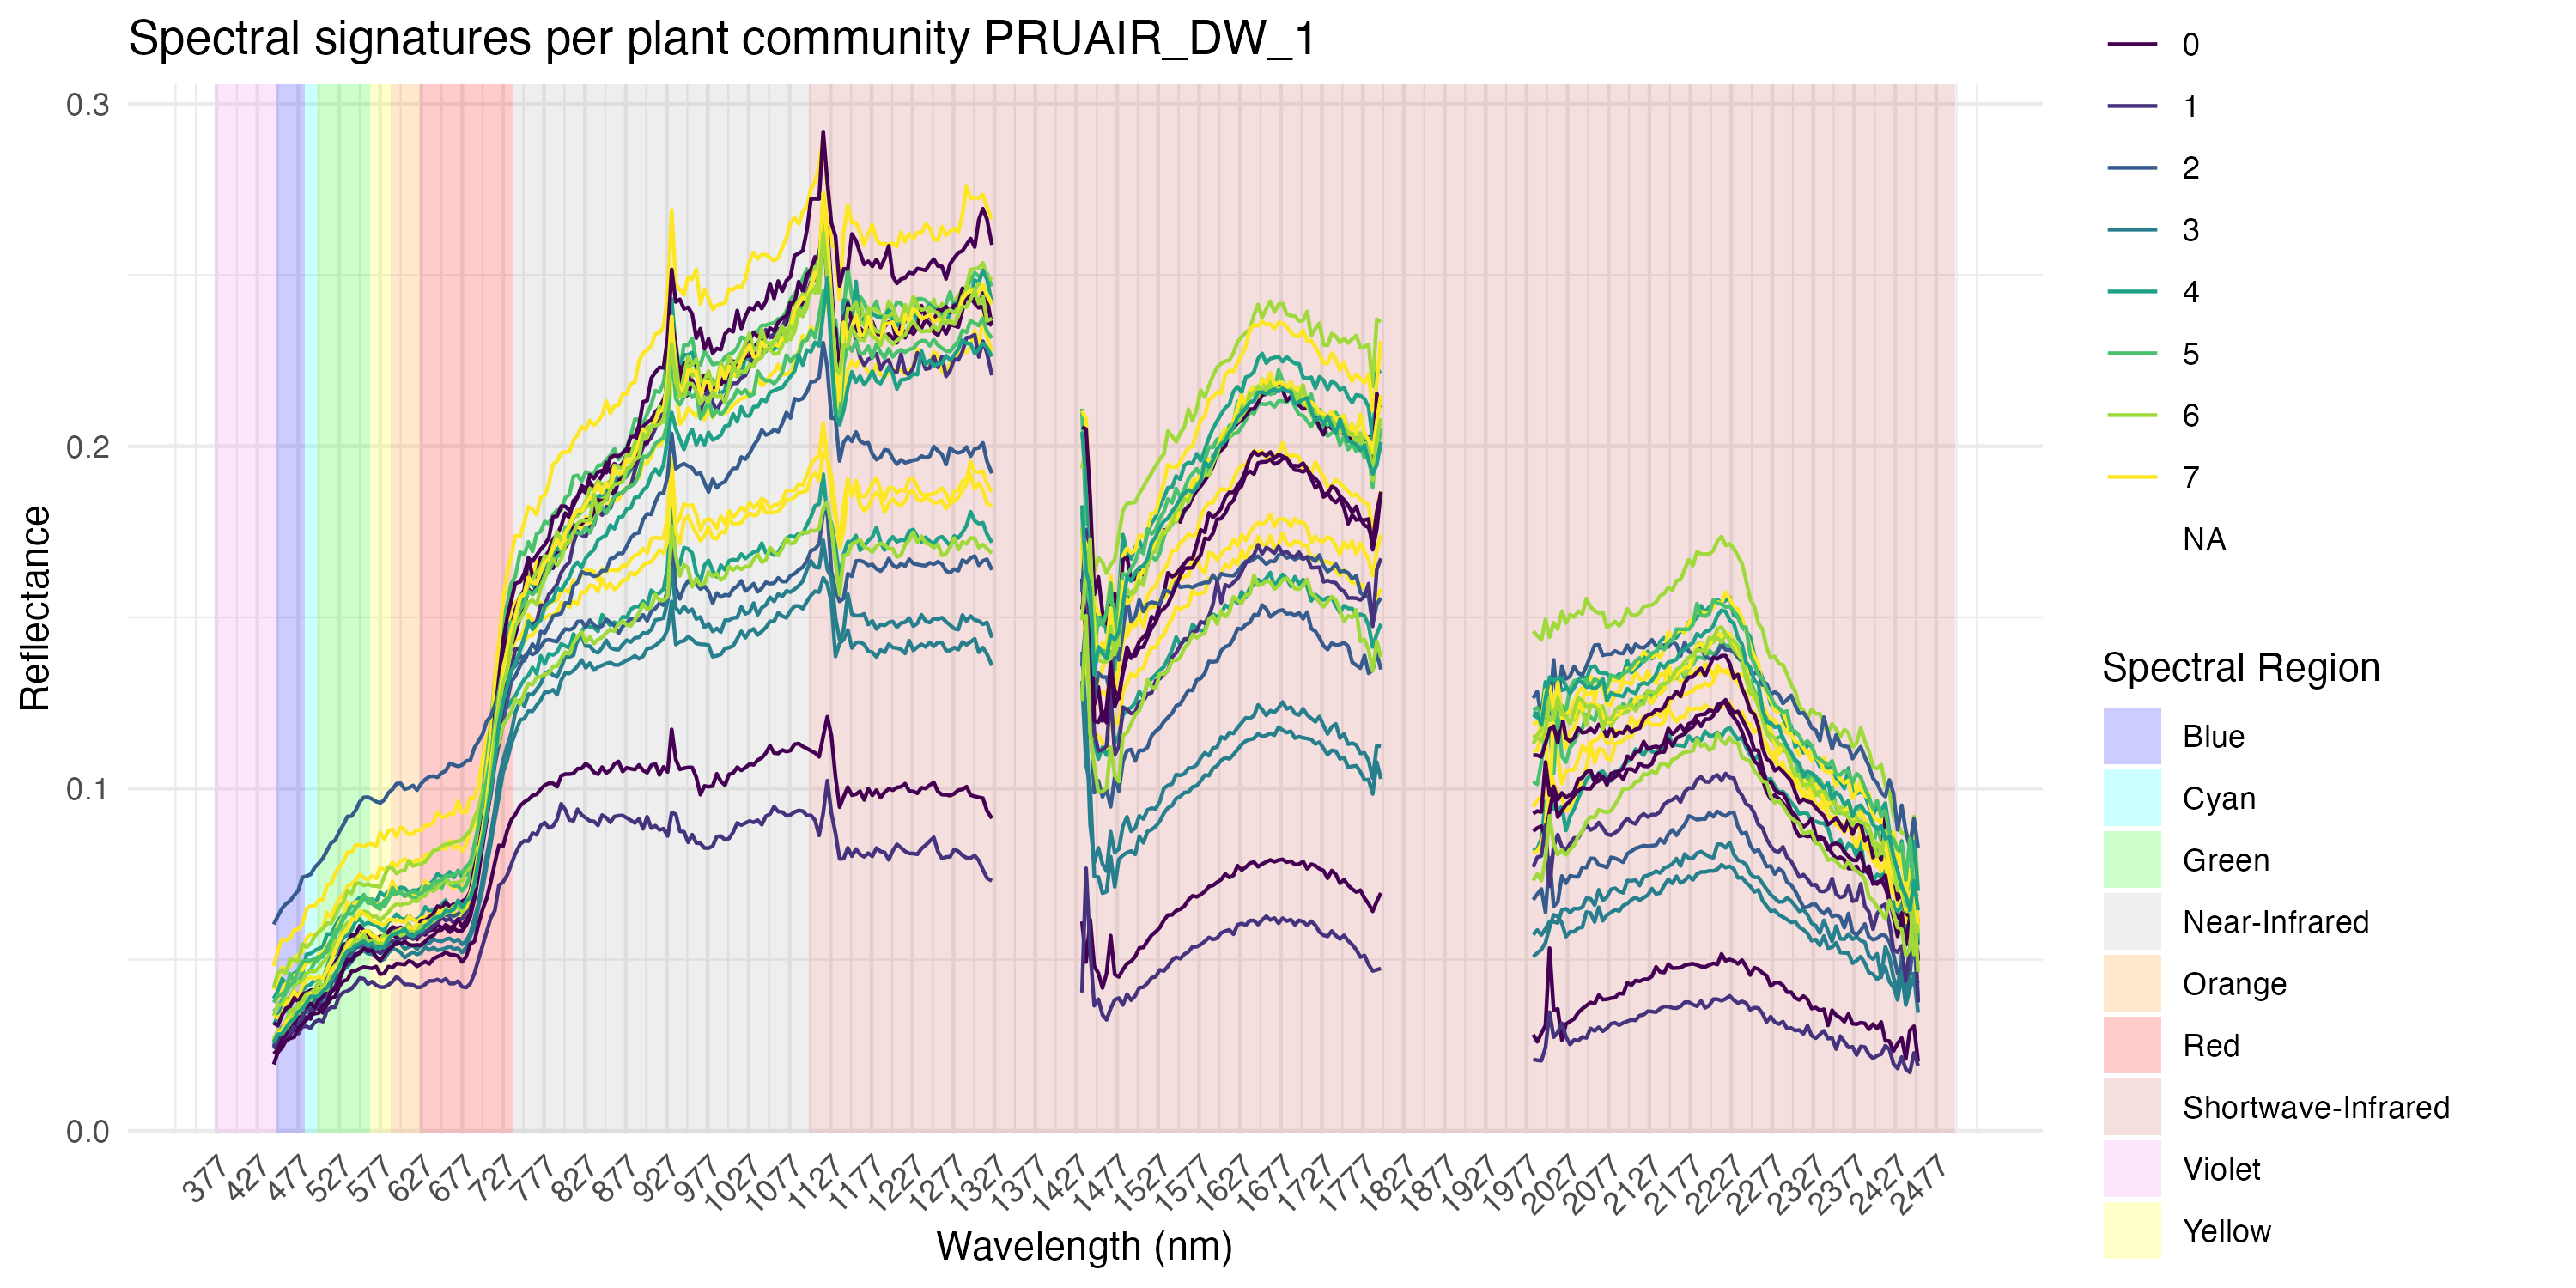
\includegraphics[width=\textwidth]{Figures/spectral_signatures/PRUAIR_DW_1_signature_plot_plant_community.png}
    \caption{}
    \label{fig:ss_pc_pruairdw1}
  \end{subfigure}
  \hfill
  \begin{subfigure}[b]{0.49\textwidth}
    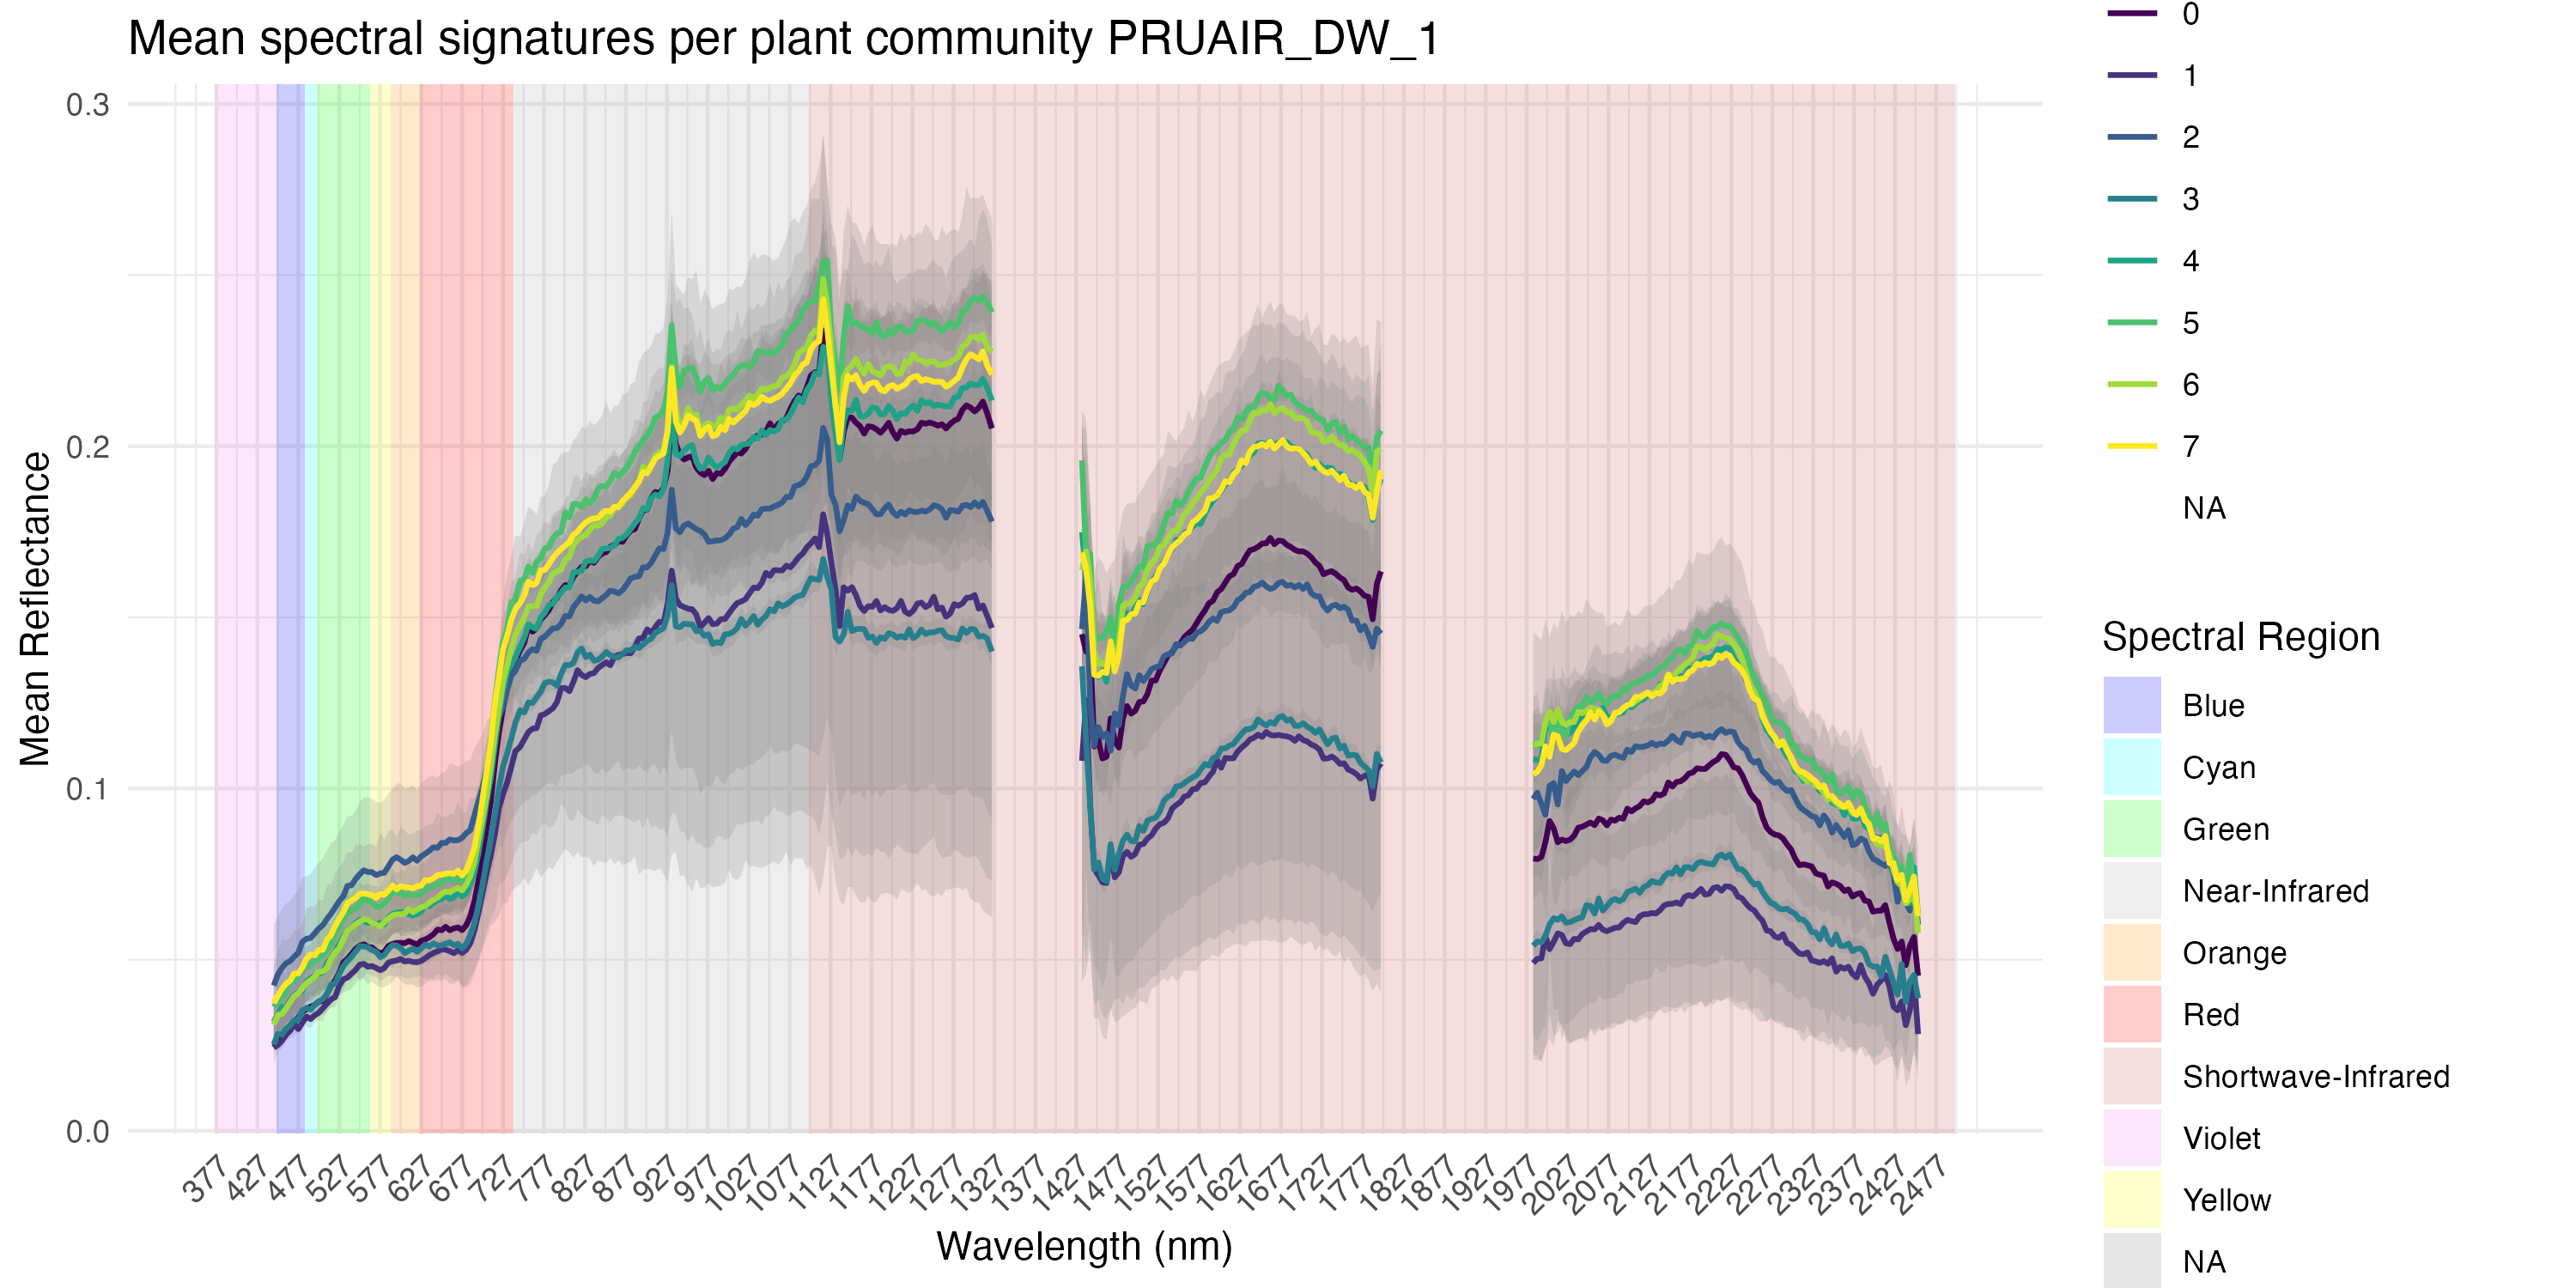
\includegraphics[width=\textwidth]{Figures/spectral_signatures/PRUAIR_DW_1_mean_signature_plot_plant_community.png}
    \caption{}
    \label{fig:mss_pc_pruairdw1}
  \end{subfigure}

  \caption{Spectral signature plot \ref{fig:ss_pc_pruairdw1} and mean spectral signature plot \ref{fig:mss_pc_pruairdw1} grouped by plant community cluster for test site PRUAIR\_DW\_1}
  \label{fig:group_pc_ht_pruairdw1}
\end{figure}

\subsection{PRUARC\_DW\_1}

\begin{figure}[H]
  \centering

  \begin{subfigure}[b]{0.49\textwidth}
    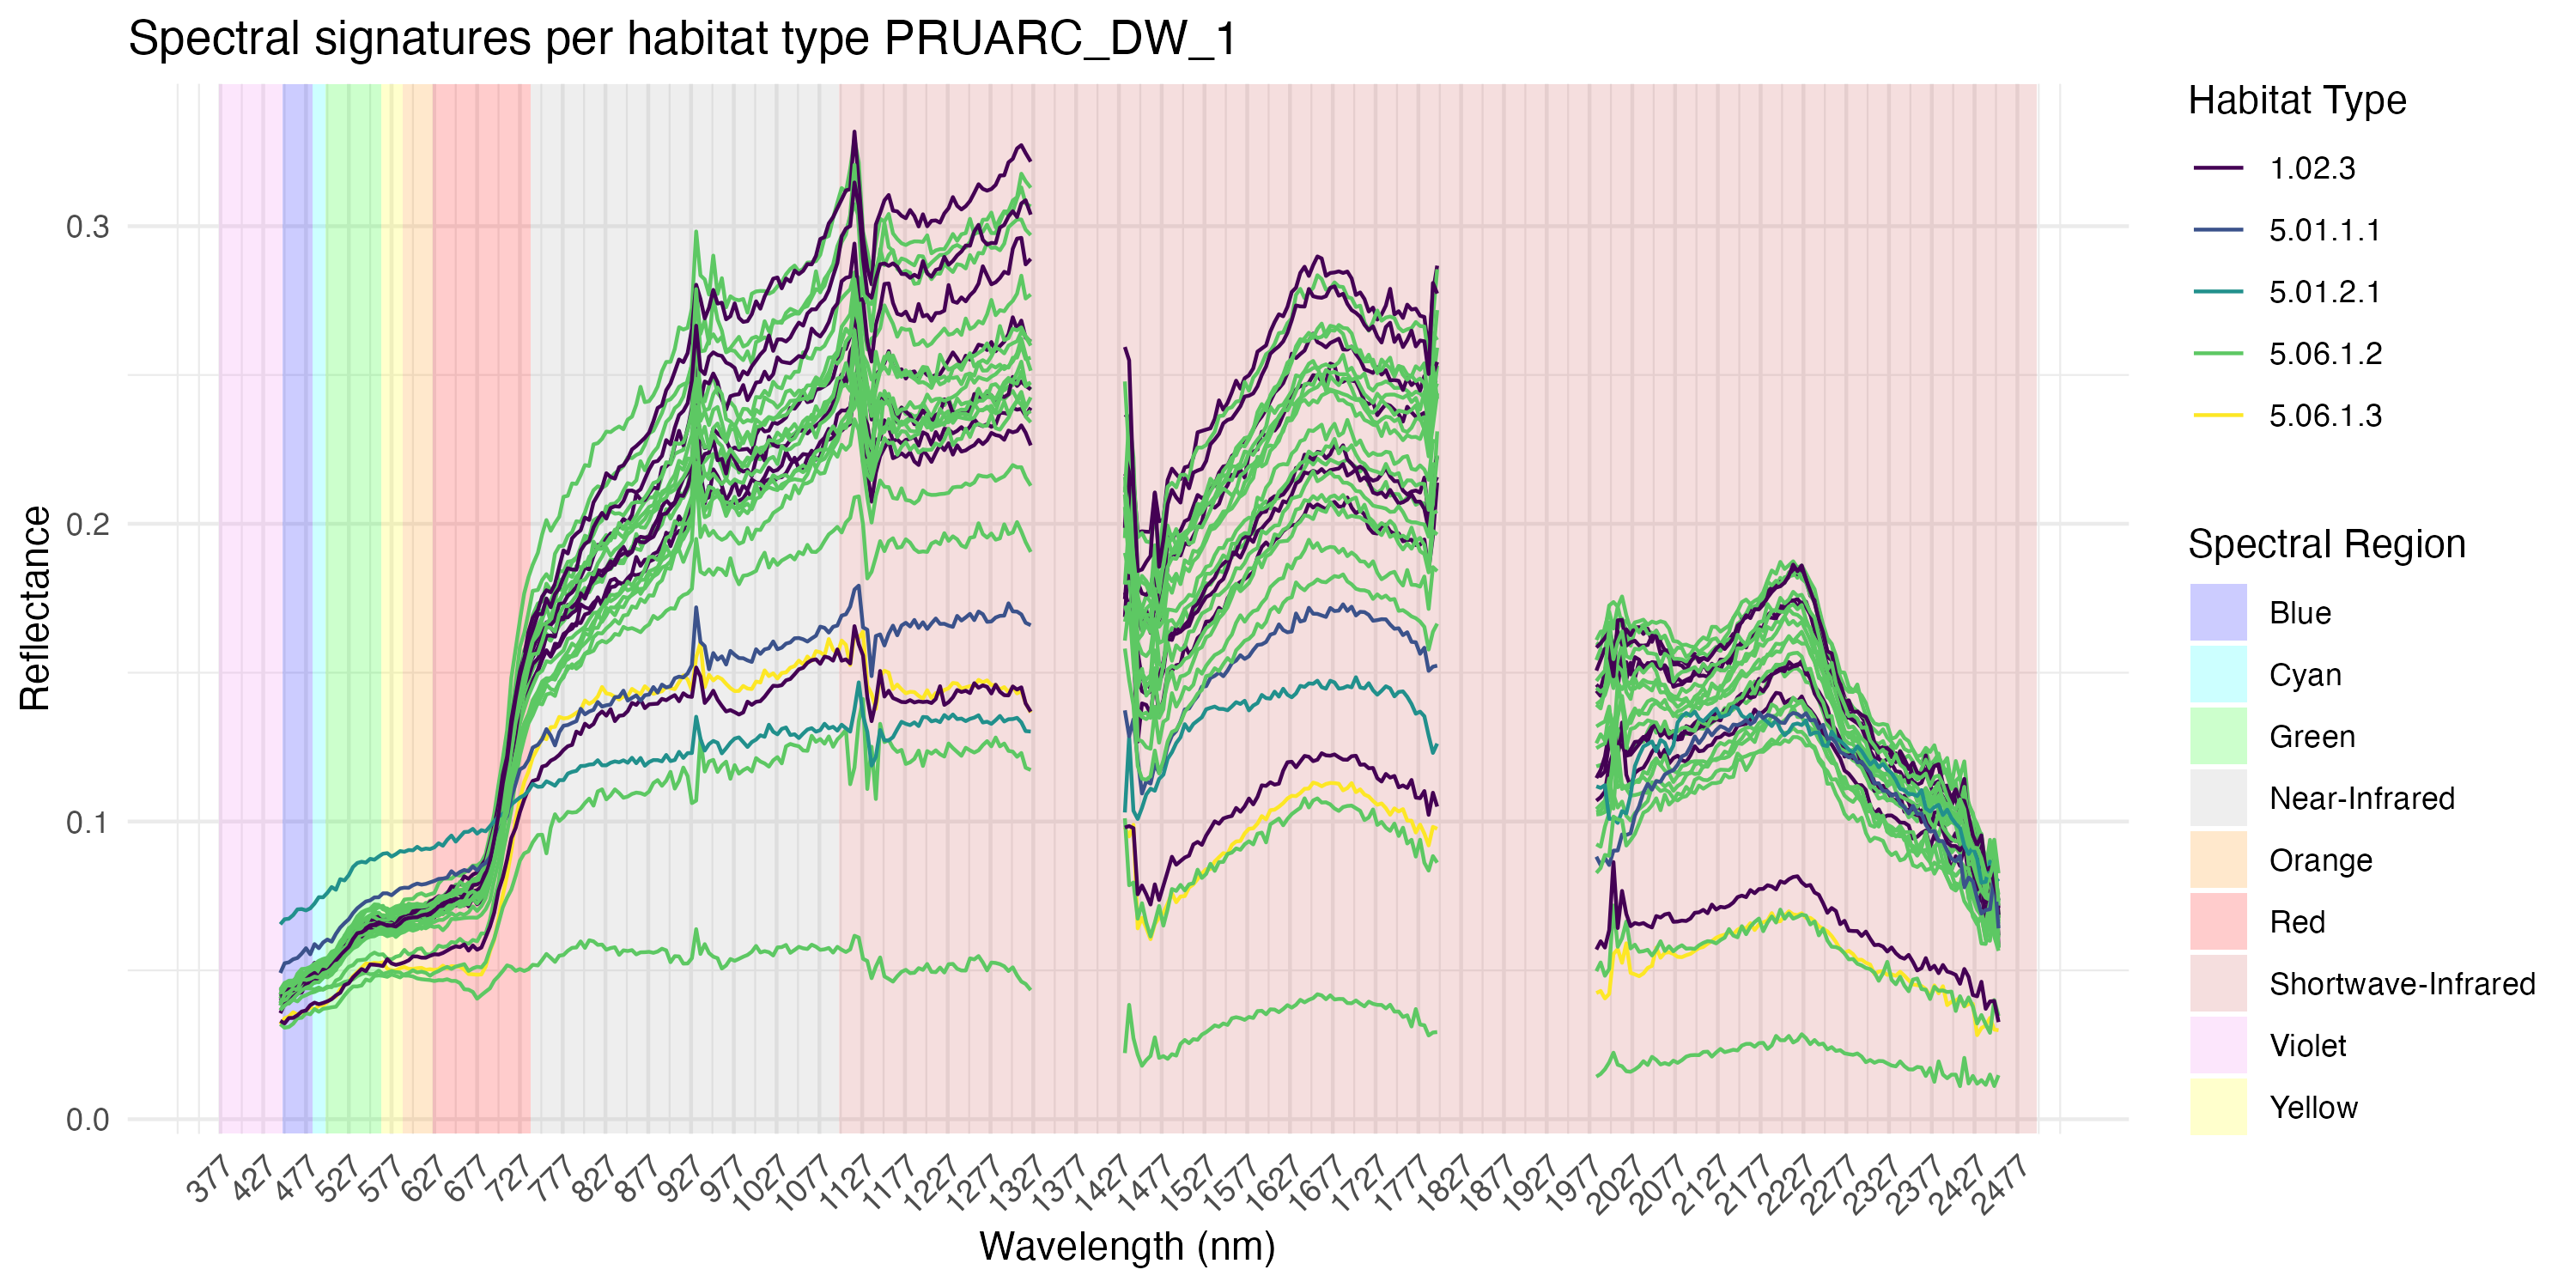
\includegraphics[width=\textwidth]{Figures/spectral_signatures/PRUARC_DW_1_signature_plot_habitat.png}
    \caption{}
    \label{fig:ss_ht_pruarcdw1}
  \end{subfigure}
  \hfill
  \begin{subfigure}[b]{0.49\textwidth}
    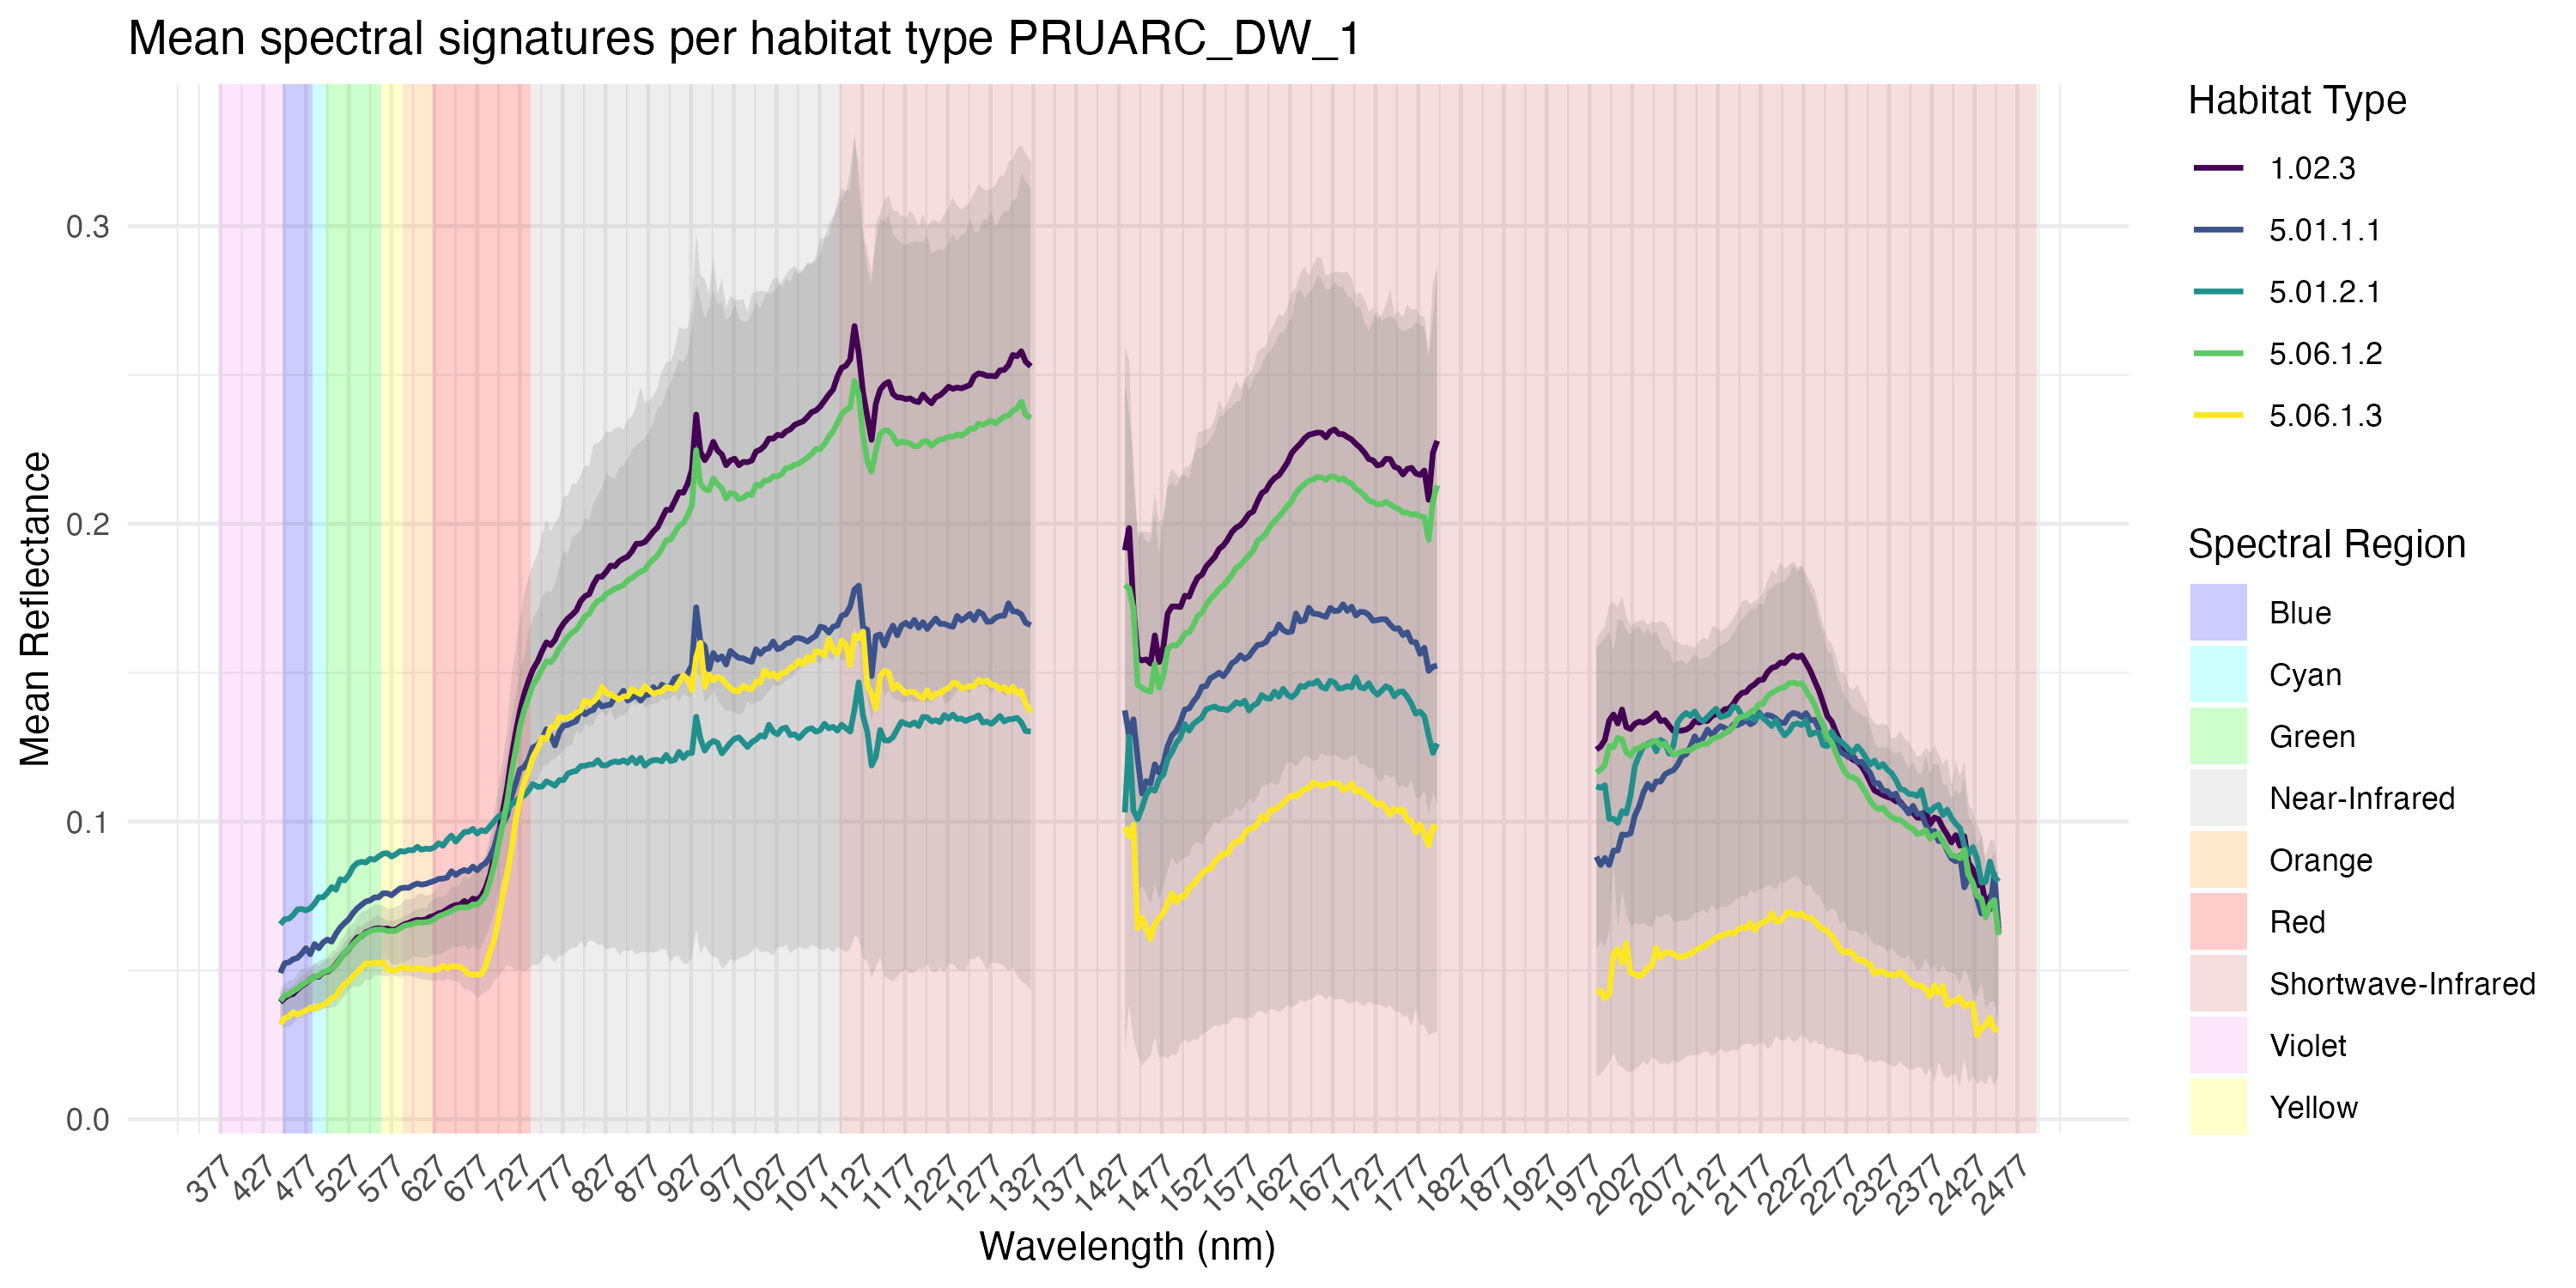
\includegraphics[width=\textwidth]{Figures/spectral_signatures/PRUARC_DW_1_mean_signature_plot_habitat.png}
    \caption{}
    \label{fig:mss_ht_pruarcdw1}
  \end{subfigure}

  \caption{Spectral signature plot \ref{fig:ss_ht_pruarcdw1} and mean spectral signature plot \ref{fig:mss_ht_pruarcdw1} grouped by habitat type for test site PRUARC\_DW\_1}
  \label{fig:group_ss_ht_pruarcdw1}
\end{figure}

\begin{figure}[H]
  \centering

  \begin{subfigure}[b]{0.49\textwidth}
    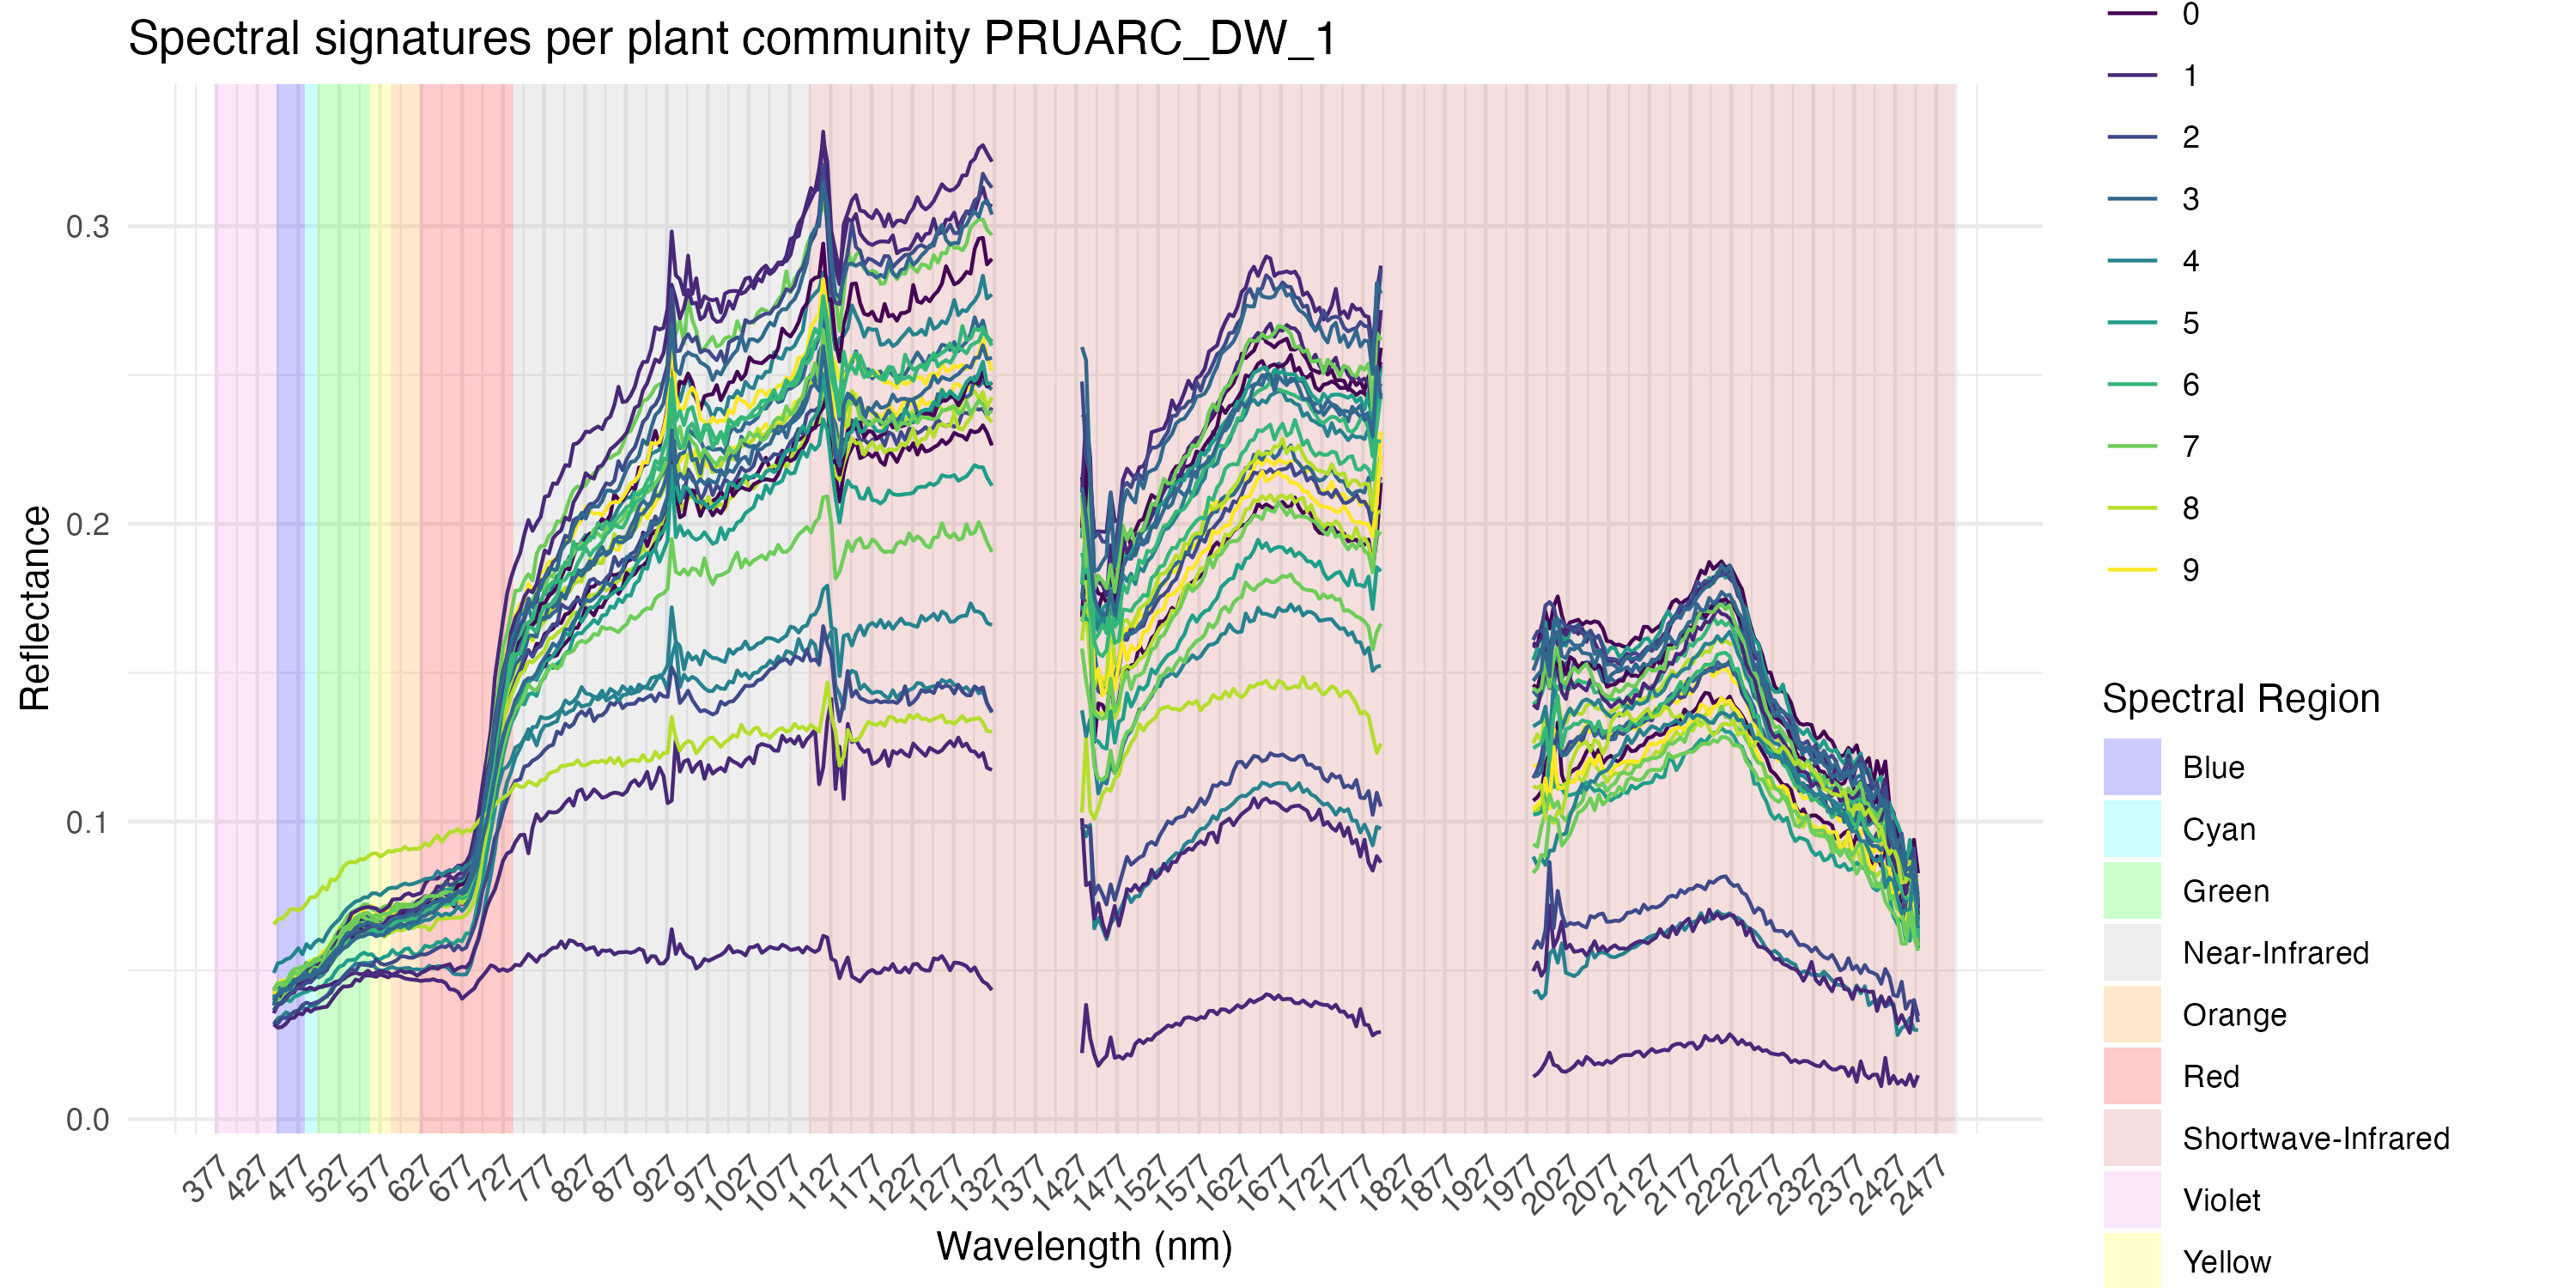
\includegraphics[width=\textwidth]{Figures/spectral_signatures/PRUARC_DW_1_signature_plot_plant_community.png}
    \caption{}
    \label{fig:ss_pc_pruarcdw1}
  \end{subfigure}
  \hfill
  \begin{subfigure}[b]{0.49\textwidth}
    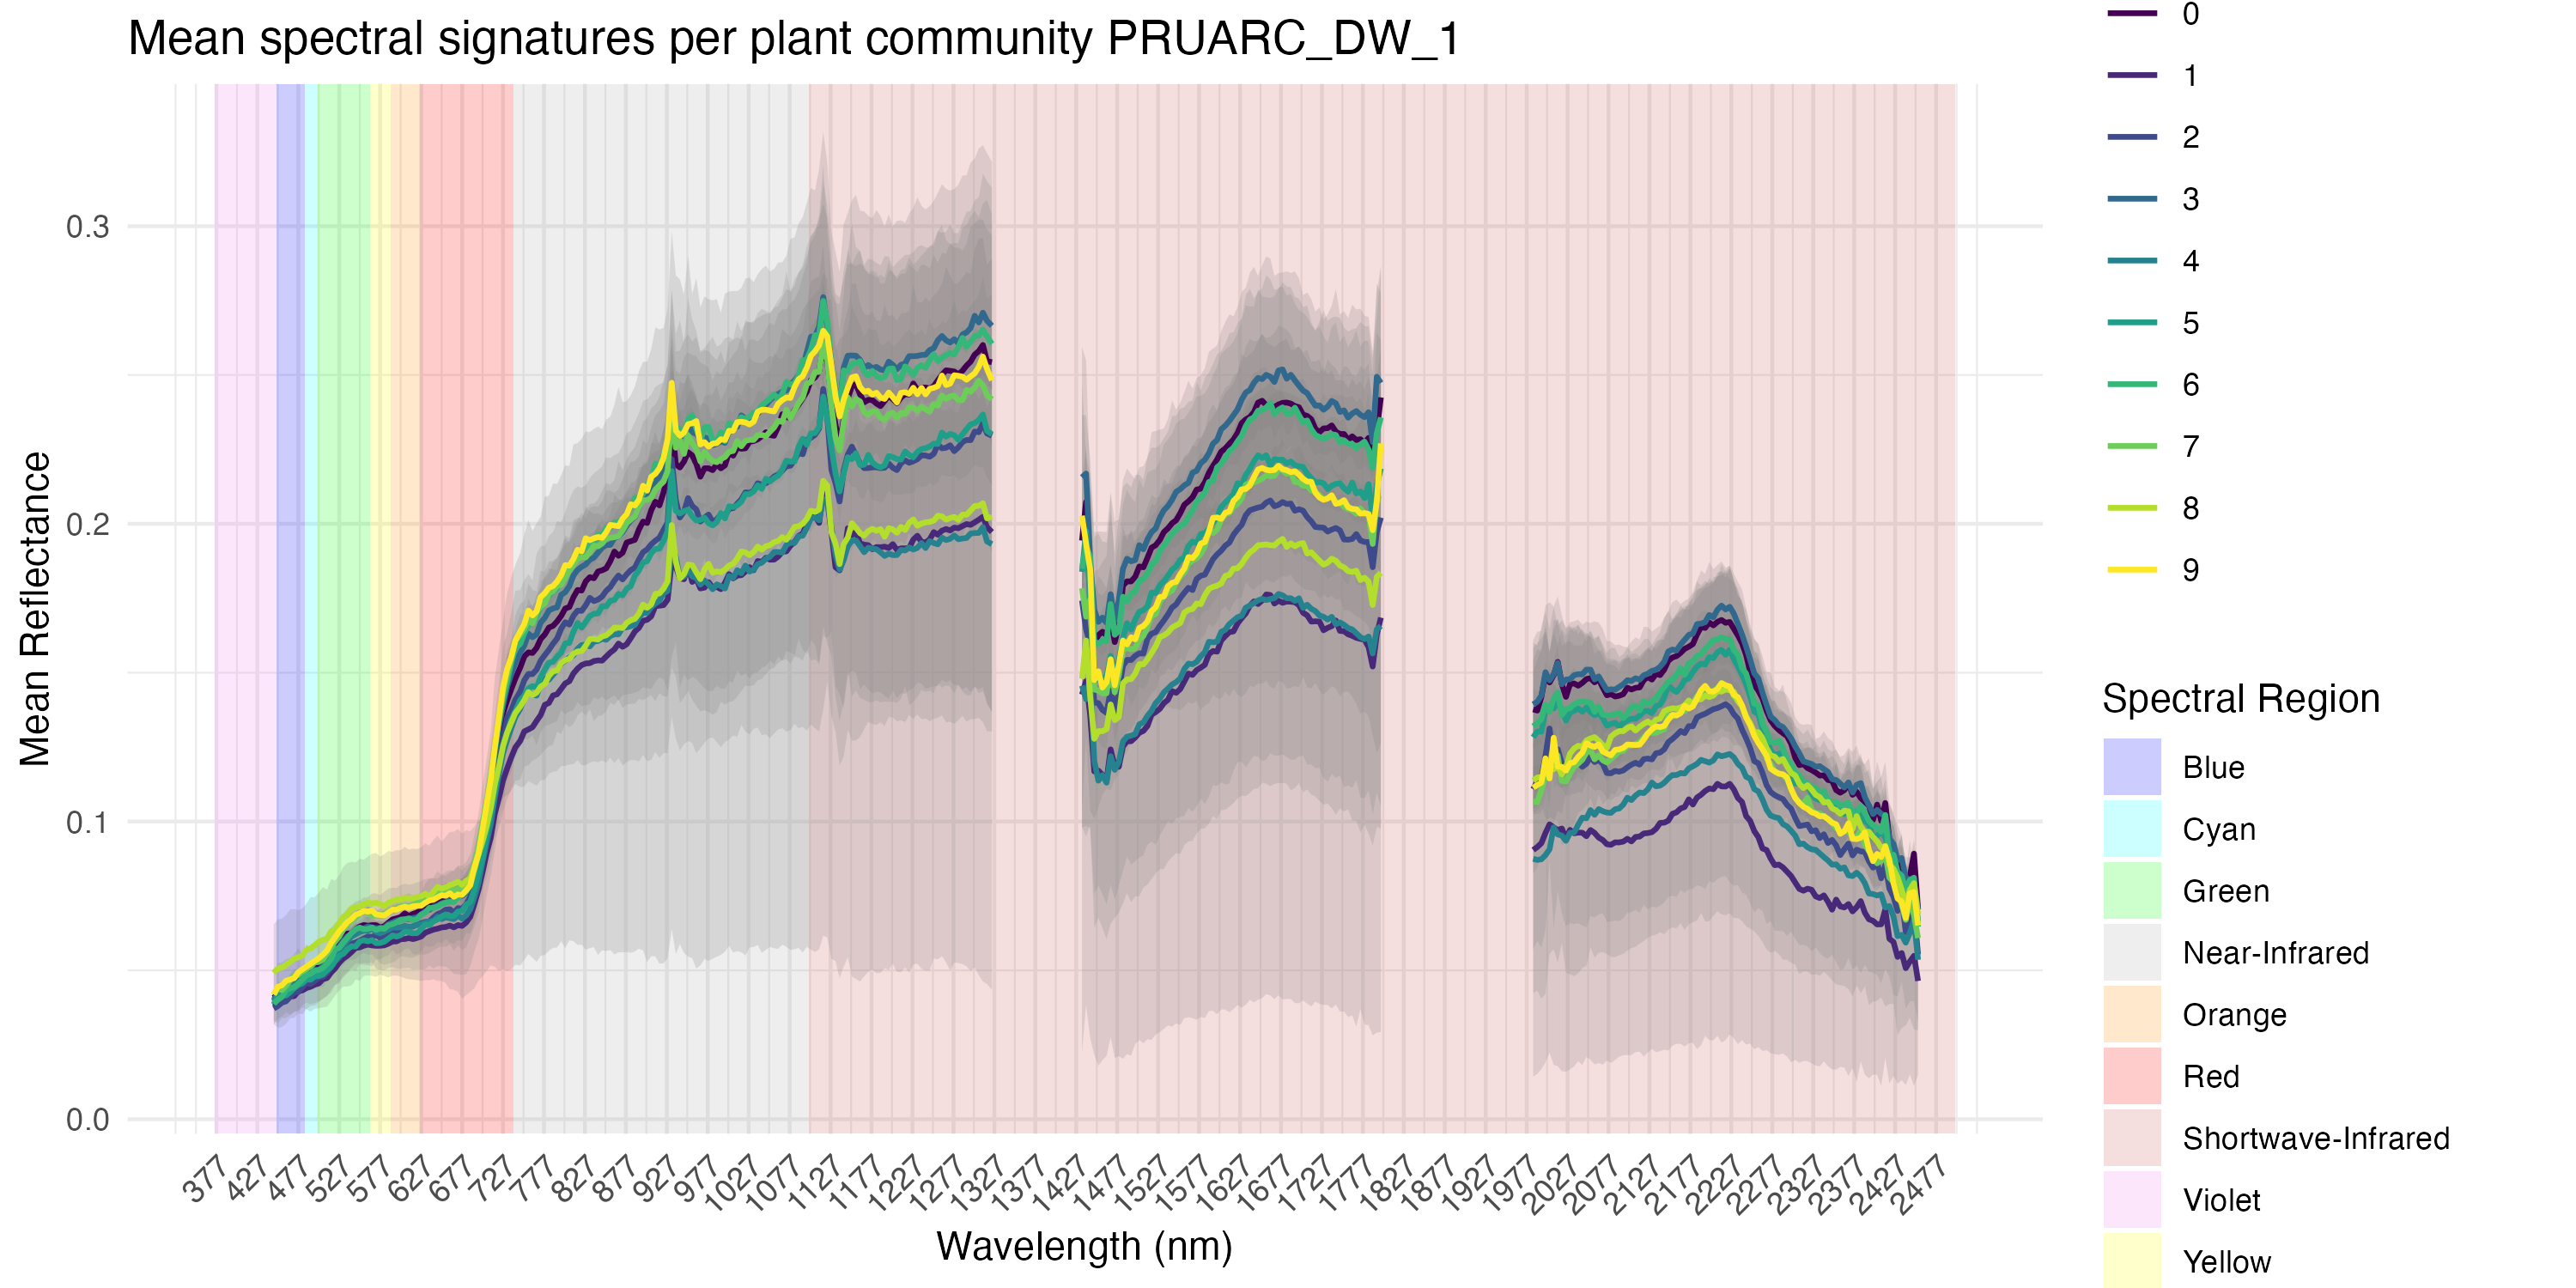
\includegraphics[width=\textwidth]{Figures/spectral_signatures/PRUARC_DW_1_mean_signature_plot_plant_community.png}
    \caption{}
    \label{fig:mss_pc_pruarcdw1}
  \end{subfigure}

  \caption{Spectral signature plot \ref{fig:ss_pc_pruarcdw1} and mean spectral signature plot \ref{fig:mss_pc_pruarcdw1} grouped by plant community cluster for test site PRUARC\_DW\_1}
  \label{fig:group_pc_ht_pruarcdw1}
\end{figure}





\subsection{Combined test sites}
In this subsection, the spectral signature lines across all the test sites were plotted grouped by habitat type.

\begin{figure}[H]
    \centering
    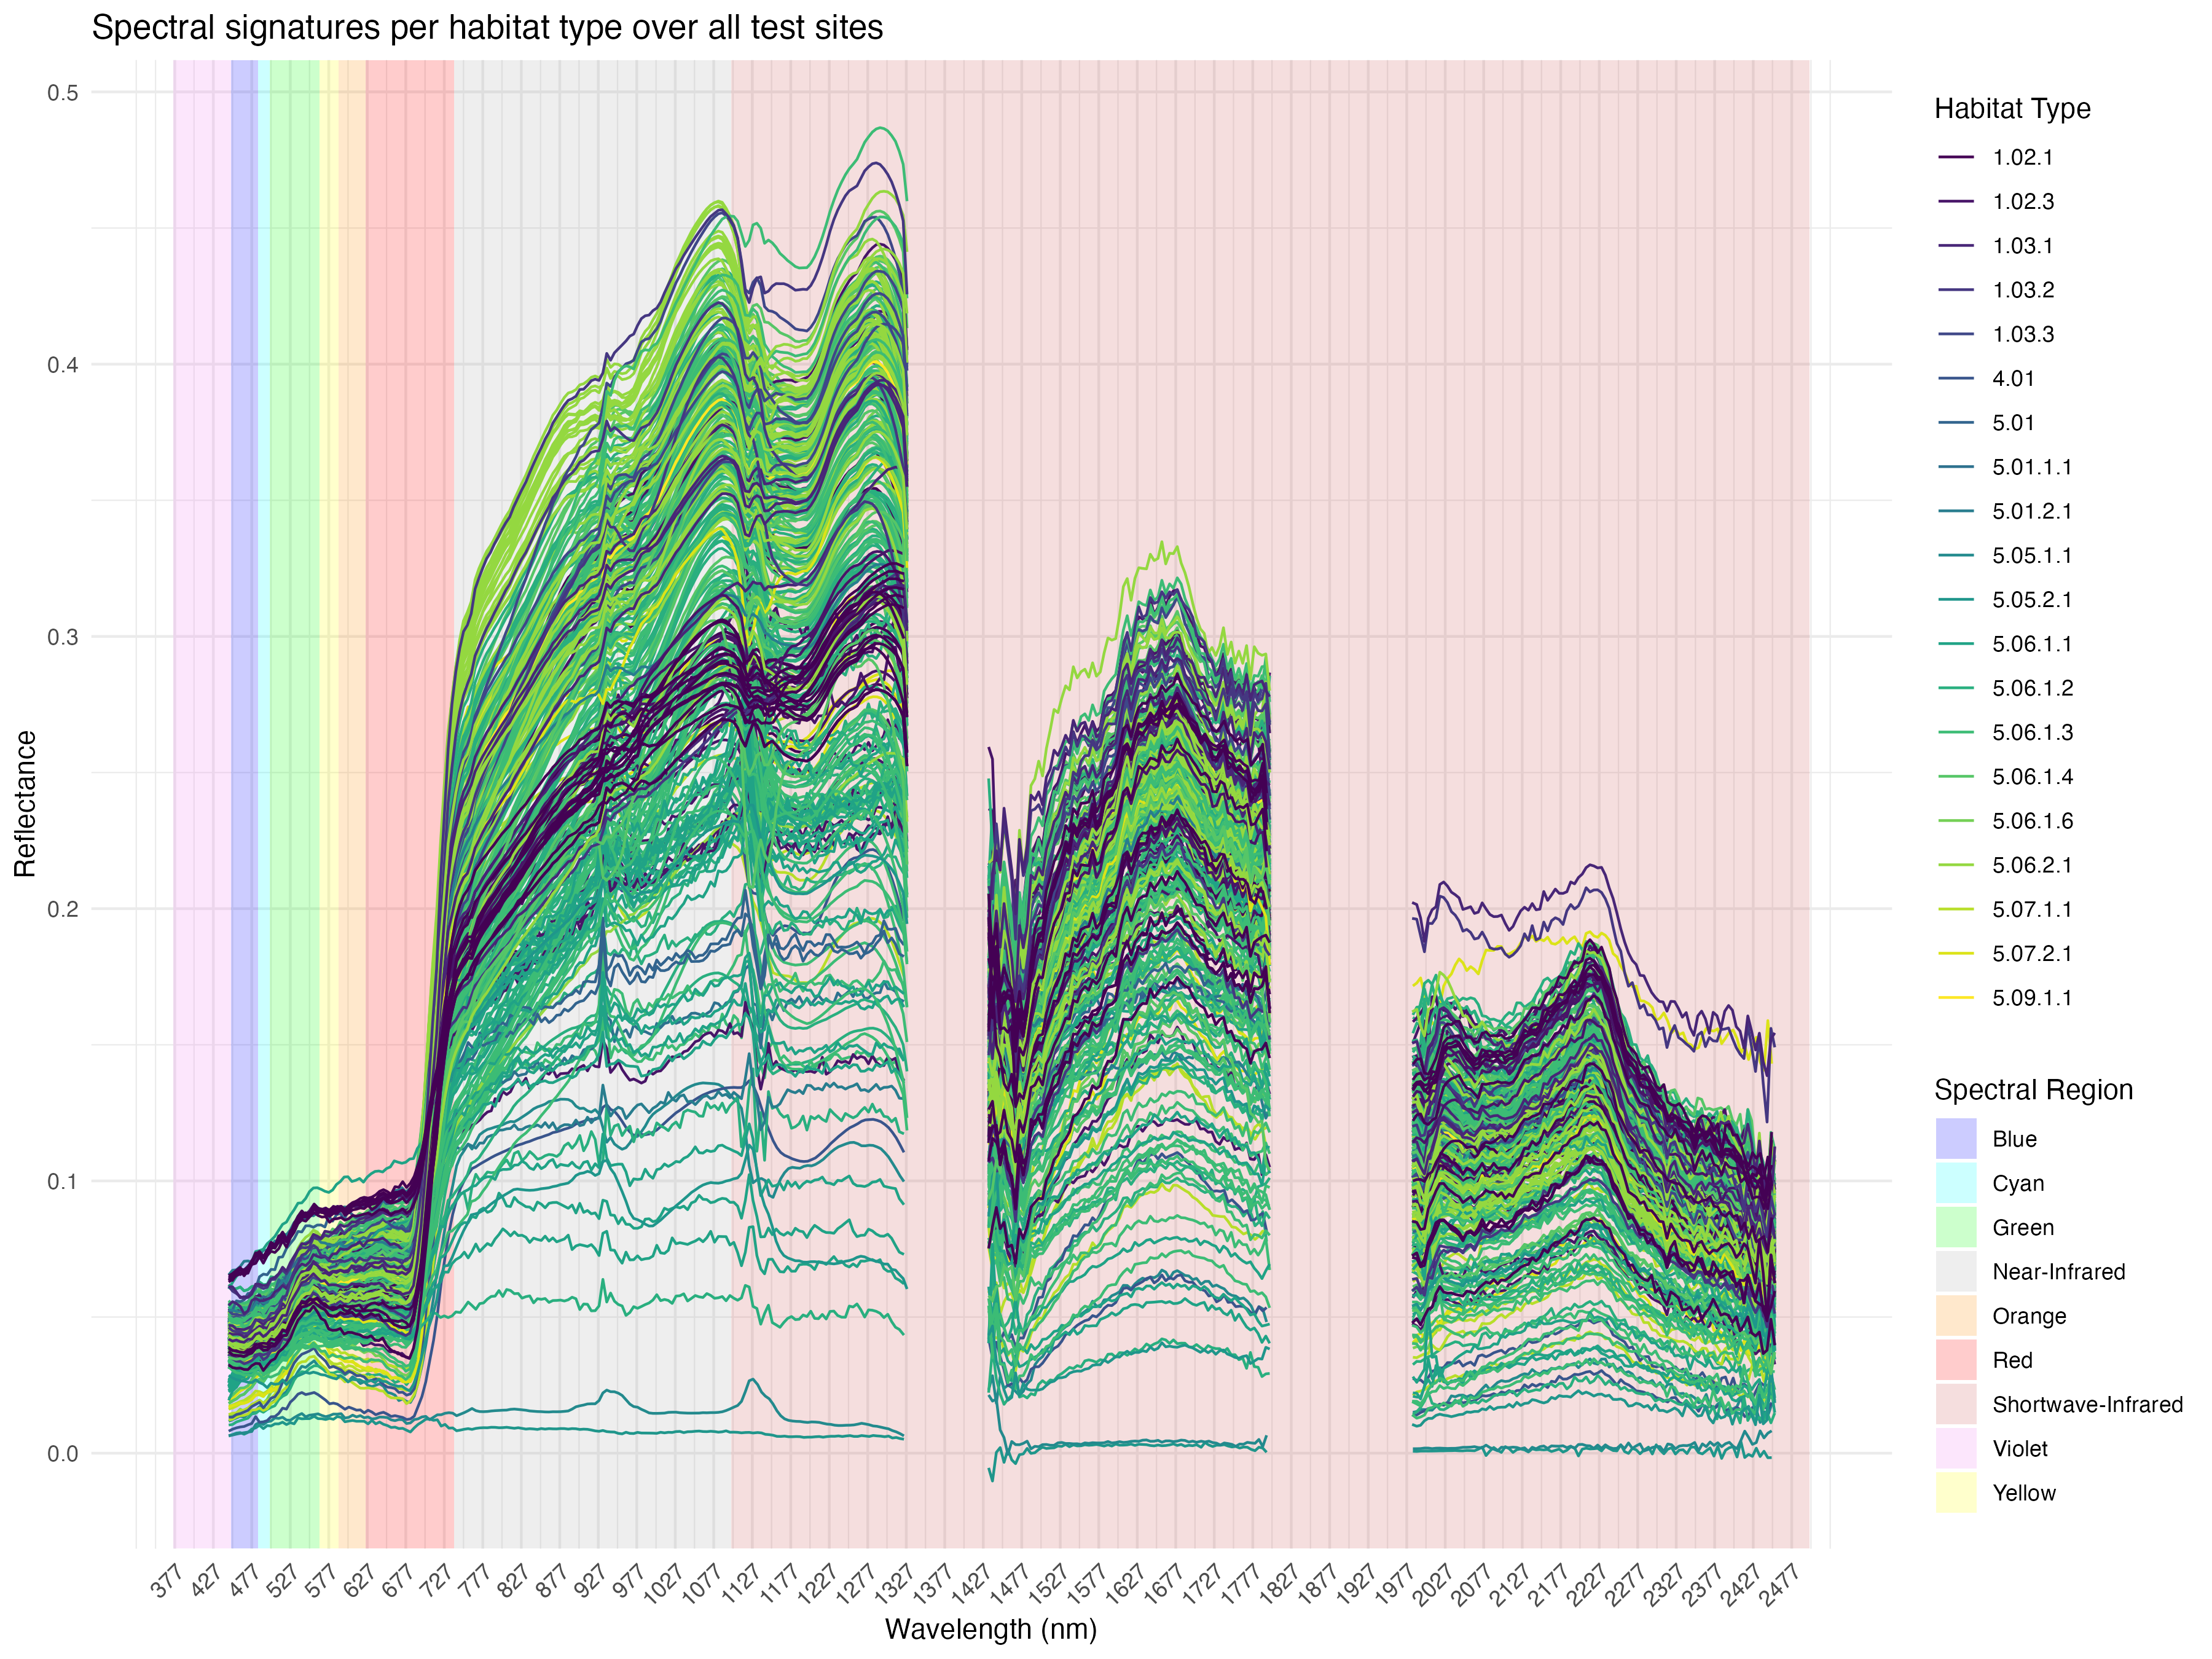
\includegraphics[width=0.9\textwidth]{Figures/spectral_signatures/All_testsites_signature_plot.png}
    \caption{The spectral signature plot over all the 354 test sites combined, grouped by habitat type}
    \label{fig:ss_all_testsites}
\end{figure}
 
%% Indicate the main file. Must go at the beginning of the file.
% !TEX root = ../main.tex

%----------------------------------------------------------------------------------------
% CHAPTER 4
%----------------------------------------------------------------------------------------



\chapter{Discussion} % Main chapter title
\label{Chapter4}

%----------------------------------------------------------------------------------------

% Define some commands to keep the formatting separated from the content
% Placing such commands in the preamble is a good idea.


%----------------------------------------------------------------------------------------

\section{Study area}
Welcome to this \LaTeX{} Thesis Template, a beautiful and easy to use template for writing a thesis using the \LaTeX{} typesetting system.

%----------------------------------------------------------------------------------------

\section{Datasets}

This section describes the different datasets that have been used for this masters thesis.

\subsection{Hyperspectral data}

This template comes as a single zip file that expands out to several files and folders. The folder names are mostly self-explanatory:

\subsection{Field data}

If you are writing a technical or mathematical thesis, then you may want to read the document by the AMS (American Mathematical Society) called, \enquote{A Short Math Guide for \LaTeX{}}. It can be found online:


%----------------------------------------------------------------------------------------

\section{Process description}

This section describes the entire process as an overview.

\subsection{Hyperspectral image pre-processing}

\subsubsection{Dimensionality reduction}

Due to the many spectral bands (425) that are captured with the AVIRIS-NG sensor, hyperspectral images can be very large and therefore a challange from a computational standpoint. To reduce

\subsubsection{Band filtering}
this and that .. bands were fitered 
insert picture etc.
%----------------------------------------------------------------------------------------

%\include{Chapters/Chapter4} 
%\include{Chapters/Chapter5} 


%----------------------------------------------------------------------------------------
% THESIS CONTENT - APPENDICES
%----------------------------------------------------------------------------------------
\appendix % Cue to tell LaTeX that the following "chapters" are Appendices

% Include the appendices of the thesis as separate files from the Appendices folder
% Uncomment the lines as you write the Appendices
%\include{Appendices/AppendixA}
% from https://www.zhaw.ch/en/lsfm/study/studiweb/master-ls/masters-thesis/
%\include{Appendices/AppendixB}
%\include{Appendices/AppendixC}
%\include{Appendices/DeclarationOfOriginalityZHAW} 

% \chapter{Linear Regression Models} % Main appendix title

\label{Appendix_LinearRegression}


\section{Plant species - spectral species}

\subsection{Results over all test sites}

\begin{table}[ht]
\centering
\caption{Summary of linear regression model predicting plant species richness from spectral species richness over all test sites}
\begin{tabular}{lcccc}
\hline
\textbf{Predictor} & \textbf{Estimate} & \textbf{Std. Error} & \textbf{t value} & \textbf{Pr($>$$|$t$|$)} \\
\hline
Intercept & 57.2577 & 18.1108 & 3.162 & \textbf{0.00905**} \\
Unique Spectral Species & 0.5489 & 0.6323 & 0.868 & 0.40390 \\
\hline
\multicolumn{5}{l}{\textit{Residual standard error:} 33.38 on 11 degrees of freedom} \\
\multicolumn{5}{l}{\textit{Multiple R-squared:} 0.06411 \quad \textit{Adjusted R-squared:} -0.02097} \\
\multicolumn{5}{l}{\textit{F-statistic:} 0.7535 on 1 and 11 DF, \quad \textit{p-value:} 0.4039} \\
\hline
\end{tabular}
\label{tab:lm_plantspecies_spectral}
\end{table}

\begin{figure}[H]
    \centering
    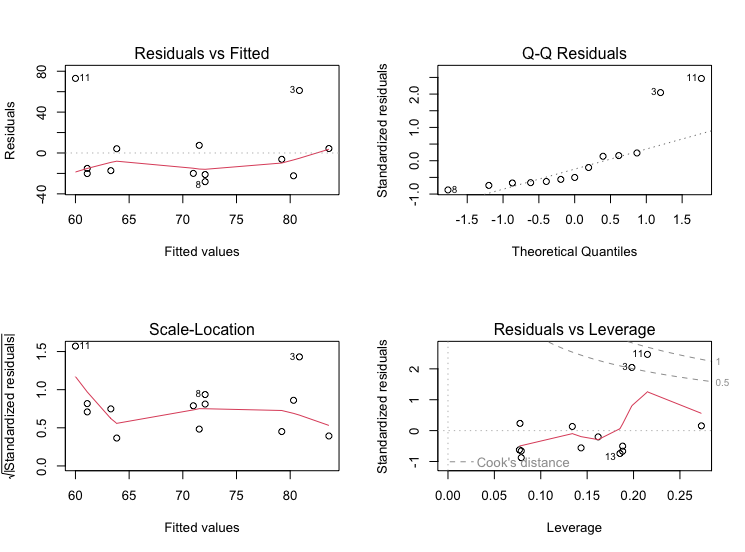
\includegraphics[width=0.9\textwidth]{Figures/Appendix/LRM_Plots/all_model_plant_species_lm.png} % Replace with your actual image path
    \caption{Residual plots for the linear regression model to predict pant species numbers from spectral species over all plots. Clear outliers are detectable in the residual vs fitted and the Q-Q residual plot (3 and 11)}
    \label{fig:all_model_plant_species_lm}
\end{figure}

\subsection{Results for Group C/D}
\begin{table}[ht]
\centering
\caption{Summary of linear regression model predicting plant species richness from spectral species richness for Group C/D}
\begin{tabular}{lcccc}
\hline
\textbf{Predictor} & \textbf{Estimate} & \textbf{Std. Error} & \textbf{t value} & \textbf{Pr($>$$|$t$|$)} \\
\hline
Intercept & 62.2493 & 25.3566 & 2.455 & \textbf{0.0396*} \\
Unique Spectral Species & 0.3982 & 0.8102 & 0.491 & 0.6363 \\
\hline
\multicolumn{5}{l}{\textit{Residual standard error:} 38.28 on 8 degrees of freedom} \\
\multicolumn{5}{l}{\textit{Multiple R-squared:} 0.02931 \quad \textit{Adjusted R-squared:} -0.09203} \\
\multicolumn{5}{l}{\textit{F-statistic:} 0.2416 on 1 and 8 DF, \quad \textit{p-value:} 0.6363} \\
\hline
\end{tabular}
\label{tab:lm_plantspecies_spectral_group_cd}
\end{table}

\begin{figure}[H]
    \centering
    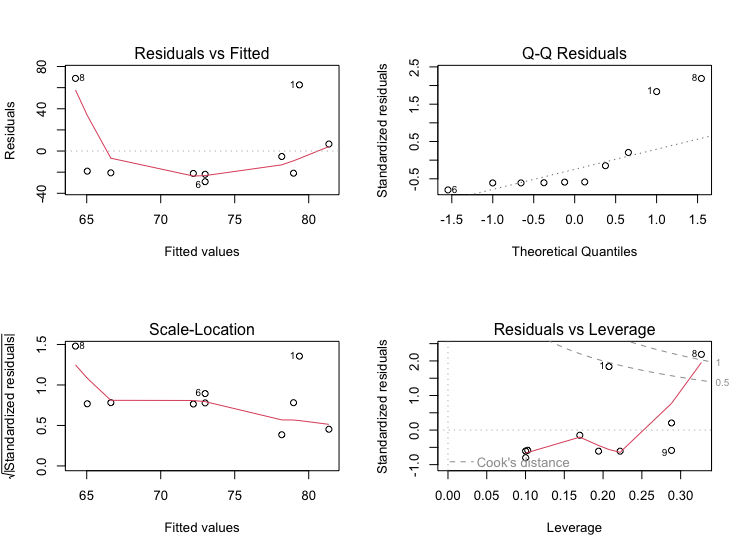
\includegraphics[width=0.9\textwidth]{Figures/Appendix/LRM_Plots/group_c_d_model_plant_species_lm.png} % Replace with your actual image path
    \caption{Residual plots for the linear regression model to predict plant species numbers from spectral species in group C/D. Clear outliers are detectable in the residual vs fitted and the Q-Q residual plot (1 and 8)}
    \label{fig:group_c_d_model_plant_species_lm}
\end{figure}

\subsection{Results for Group E}
\begin{table}[ht]
\centering
\caption{Summary of linear regression model predicting plant species richness from spectral species richness for Group E}
\begin{tabular}{lcccc}
\hline
\textbf{Predictor} & \textbf{Estimate} & \textbf{Std. Error} & \textbf{t value} & \textbf{Pr($>$$|$t$|$)} \\
\hline
Intercept & 36.6100 & 16.3602 & 2.238 &  0.268 \\
Unique Spectral Species & 1.7371 & 0.9613 & 1.807 & 0.322 \\
\hline
\multicolumn{5}{l}{\textit{Residual standard error:} 13.39 on 1 degrees of freedom} \\
\multicolumn{5}{l}{\textit{Multiple R-squared:} 0.7656 \quad \textit{Adjusted R-squared:} 0.5311} \\
\multicolumn{5}{l}{\textit{F-statistic:} 3.266 on 1 and 1 DF, \quad \textit{p-value:} 0.3218} \\
\hline
\end{tabular}
\label{tab:lm_plantspecies_spectral_group_e}
\end{table}

\begin{figure}[H]
    \centering
    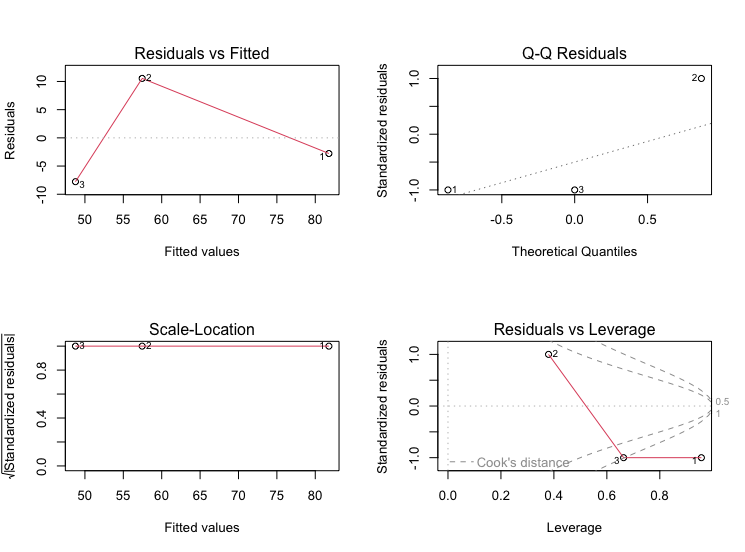
\includegraphics[width=0.9\textwidth]{Figures/Appendix/LRM_Plots/group_e_model_plant_species_lm.png} % Replace with your actual image path
    \caption{Residual plots for the linear regression model to predict plant species numbers from spectral species in group E. Since there are so few data points the the results don't hold any value.}
    \label{fig:group_e_model_plant_species_lm}
\end{figure}


\section{Plant communities - spectral species}
\subsection{Results over all test sites}
\begin{table}[ht]
\centering
\caption{Summary of linear regression model predicting plant community richness from spectral species richness over all test sites}
\begin{tabular}{lcccc}
\hline
\textbf{Predictor} & \textbf{Estimate} & \textbf{Std. Error} & \textbf{t value} & \textbf{Pr($>$$|$t$|$)} \\
\hline
Intercept & 9.08876 & 2.53324 & 3.588 & \textbf{0.00426**} \\
Unique Spectral Species & -0.02236 & 0.08845 & -0.253 & 0.80512 \\
\hline
\multicolumn{5}{l}{\textit{Residual standard error:} 4.669 on 11 degrees of freedom} \\
\multicolumn{5}{l}{\textit{Multiple R-squared:} 0.005774 \quad \textit{Adjusted R-squared:} -0.08461} \\
\multicolumn{5}{l}{\textit{F-statistic:} 0.06389 on 1 and 11 DF, \quad \textit{p-value:} 0.8051} \\
\hline
\end{tabular}
\label{tab:lm_plant_community_spectral}
\end{table}

\begin{figure}[H]
    \centering
    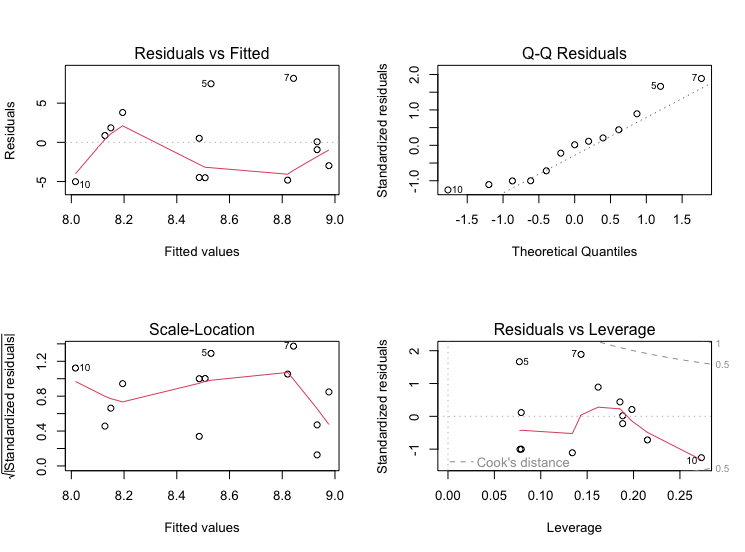
\includegraphics[width=0.9\textwidth]{Figures/Appendix/LRM_Plots/all_model_plant_communities_lm.png} % Replace with your actual image path
    \caption{Residual plots for the linear regression model to predict plant community numbers from spectral species over all plots.}
    \label{fig:all_model_plant_communities_lm}
\end{figure}

\subsection{Results for Group C/D}
\begin{table}[ht]
\centering
\caption{Summary of linear regression model predicting plant community richness from spectral species richness for Group C/D}
\begin{tabular}{lcccc}
\hline
\textbf{Predictor} & \textbf{Estimate} & \textbf{Std. Error} & \textbf{t value} & \textbf{Pr($>$$|$t$|$)} \\
\hline
Intercept & 11.00134 & 3.18381 & 3.455 & \textbf{0.00863**} \\
Unique Spectral Species & -0.05823 & 0.10173 & -0.572 & 0.58277 \\
\hline
\multicolumn{5}{l}{\textit{Residual standard error:} 4.807 on 8 degrees of freedom} \\
\multicolumn{5}{l}{\textit{Multiple R-squared:} 0.03935 \quad \textit{Adjusted R-squared:} -0.08074} \\
\multicolumn{5}{l}{\textit{F-statistic:} 0.3277 on 1 and 8 DF, \quad \textit{p-value:} 0.5828} \\
\hline
\end{tabular}
\label{tab:lm_plantspecies_spectral}
\end{table}

\begin{figure}[H]
    \centering
    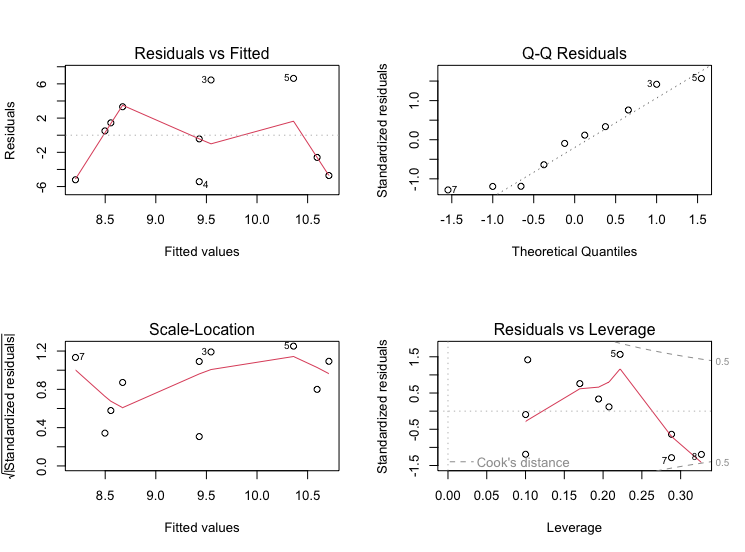
\includegraphics[width=0.9\textwidth]{Figures/Appendix/LRM_Plots/group_c_d_model_plant_communities_lm.png} % Replace with your actual image path
    \caption{Residual plots for the linear regression model to predict plant community numbers from spectral species in group C/D.}
    \label{fig:group_c_d_model_plant_communities_lm}
\end{figure}

\subsection{Results for Group E}
\begin{table}[ht]
\centering
\caption{Summary of linear regression model predicting plant community richness from spectral species richness for Group E}
\begin{tabular}{lcccc}
\hline
\textbf{Predictor} & \textbf{Estimate} & \textbf{Std. Error} & \textbf{t value} & \textbf{Pr($>$$|$t$|$)} \\
\hline
Intercept & 8.7595 & 3.5456 & 2.471 & 0.245 \\
Unique Spectral Species & -0.2062 & 0.2083 & -0.990 & 0.503 \\
\hline
\multicolumn{5}{l}{\textit{Residual standard error:} 2.902 on 1 degrees of freedom} \\
\multicolumn{5}{l}{\textit{Multiple R-squared:} 0.4948 \quad \textit{Adjusted R-squared:} -0.01031} \\
\multicolumn{5}{l}{\textit{F-statistic:} 0.9796 on 1 and 1 DF, \quad \textit{p-value:} 0.5033} \\
\hline
\end{tabular}
\label{tab:lm_plantspecies_spectral}
\end{table}

\begin{figure}[H]
    \centering
    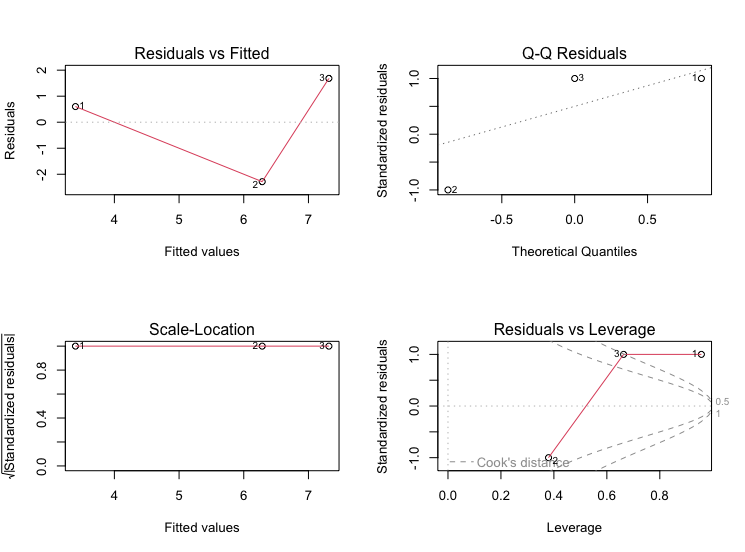
\includegraphics[width=0.9\textwidth]{Figures/Appendix/LRM_Plots/group_e_model_plant_communities_lm.png} % Replace with your actual image path
    \caption{Residual plots for the linear regression model to predict plant community numbers from spectral species in group E.}
    \label{fig:group_e_model_plant_communities_lm}
\end{figure}

\section{Habitat types - spectral species}
\begin{table}[ht]
\centering
\caption{Summary of linear regression model predicting habitat type richness from spectral species richness over all test sites}
\begin{tabular}{lcccc}
\hline
\textbf{Predictor} & \textbf{Estimate} & \textbf{Std. Error} & \textbf{t value} & \textbf{Pr($>$$|$t$|$)} \\
\hline
Intercept & 2.94635 & 0.86879 & 3.391 & \textbf{0.00602**} \\
Unique Spectral Species & 0.03030 & 0.03033 & 0.999 & 0.33925 \\
\hline
\multicolumn{5}{l}{\textit{Residual standard error:} 1.601 on 11 degrees of freedom} \\
\multicolumn{5}{l}{\textit{Multiple R-squared:} 0.08319 \quad \textit{Adjusted R-squared:} -0.0001603} \\
\multicolumn{5}{l}{\textit{F-statistic:} 0.9981 on 1 and 11 DF, \quad \textit{p-value:} 0.3392} \\
\hline
\end{tabular}
\label{tab:lm_habitat_type_spectral}
\end{table}

\begin{figure}[H]
    \centering
    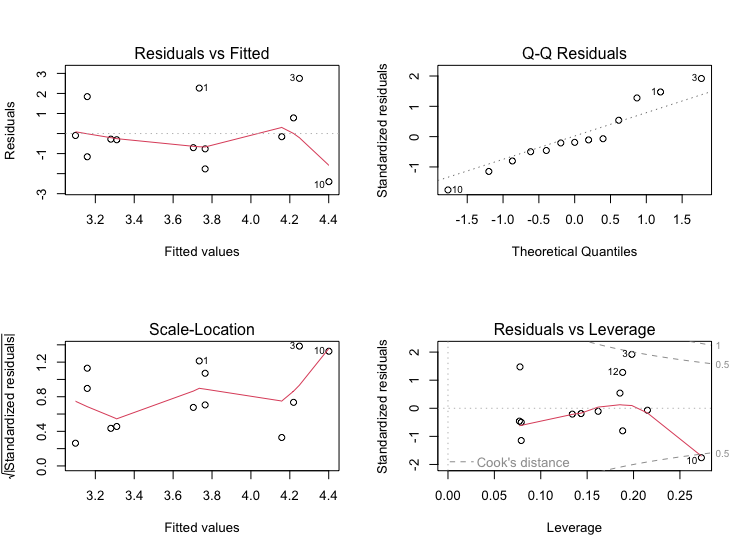
\includegraphics[width=0.9\textwidth]{Figures/Appendix/LRM_Plots/all_model_habitat_types_lm.png} % Replace with your actual image path
    \caption{Residual plots for the linear regression model to predict habitat type numbers from spectral species over all plots.}
    \label{fig:all_model_habitat_types_lm}
\end{figure}


\subsection{Results for Group C/D}
\begin{table}[ht]
\centering
\caption{Summary of linear regression model predicting habitat type richness from spectral species richness for Group C/D}
\begin{tabular}{lcccc}
\hline
\textbf{Predictor} & \textbf{Estimate} & \textbf{Std. Error} & \textbf{t value} & \textbf{Pr($>$$|$t$|$)} \\
\hline
Intercept & 3.17648 & 1.08058 & 2.940 & \textbf{0.0187*} \\
Unique Spectral Species & 0.01904 & 0.03453 & 0.551 & 0.5964 \\
\hline
\multicolumn{5}{l}{\textit{Residual standard error:} 1.631 on 8 degrees of freedom} \\
\multicolumn{5}{l}{\textit{Multiple R-squared:} 0.03661 \quad \textit{Adjusted R-squared:} -0.08381} \\
\multicolumn{5}{l}{\textit{F-statistic:} 0.304 on 1 and 8 DF, \quad \textit{p-value:} 0.5964} \\
\hline
\end{tabular}
\label{tab:lm_plantspecies_spectral}
\end{table}

\begin{figure}[H]
    \centering
    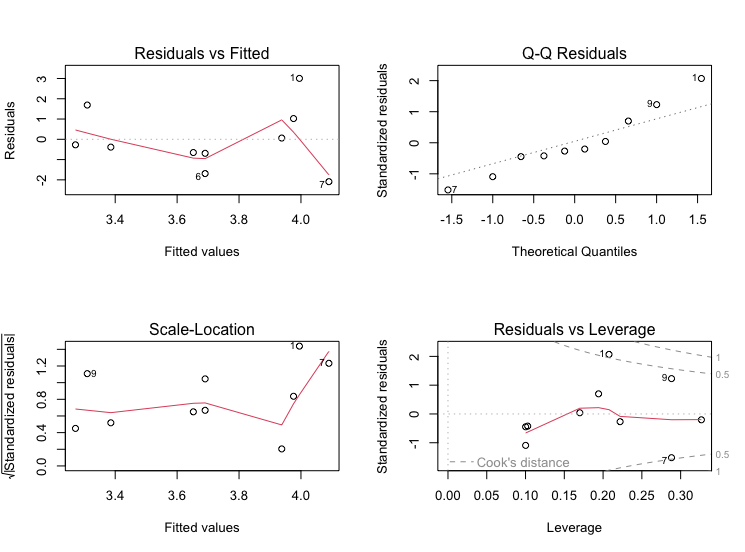
\includegraphics[width=0.9\textwidth]{Figures/Appendix/LRM_Plots/group_c_d_model_habitat_types_lm.png} % Replace with your actual image path
    \caption{Residual plots for the linear regression model to predict habitat type numbers from spectral species in group C/D.}
    \label{fig:group_c_d_model_habitat_types_lm}
\end{figure}

\subsection{Results for Group E}
\begin{table}[ht]
\centering
\caption{Summary of linear regression model predicting habitat type richness from spectral species richness for Group E}
\begin{tabular}{lcccc}
\hline
\textbf{Predictor} & \textbf{Estimate} & \textbf{Std. Error} & \textbf{t value} & \textbf{Pr($>$$|$t$|$)} \\
\hline
Intercept & 0.496564 & 0.050651 & 9.804 & 0.06471 \\
Unique Spectral Species & 0.211340 & 0.002976 & 71.014 & \textbf{0.00896**} \\
\hline
\multicolumn{5}{l}{\textit{Residual standard error:} 0.04145 on 1 degrees of freedom} \\
\multicolumn{5}{l}{\textit{Multiple R-squared:} 0.9998 \quad \textit{Adjusted R-squared:} 0.9996} \\
\multicolumn{5}{l}{\textit{F-statistic:} 5043 on 1 and 1 DF, \quad \textit{p-value:} 0.008964} \\
\hline
\end{tabular}
\label{tab:lm_plantspecies_spectral}
\end{table}

\begin{figure}[H]
    \centering
    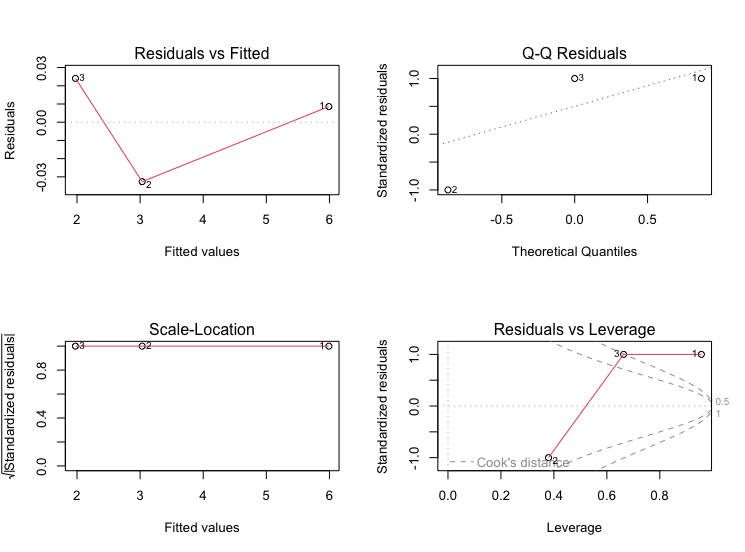
\includegraphics[width=0.9\textwidth]{Figures/Appendix/LRM_Plots/group_e_model_habitat_types_lm.png} % Replace with your actual image path
    \caption{Residual plots for the linear regression model to predict habitat type numbers from spectral species in group E.}
    \label{fig:group_e_model_habitat_types_lm}
\end{figure}
% \chapter{Plant Community Clustering} % Main appendix title

\label{Appendix_PlantCommunityClustering}

\section{HDBSCAN cluster plots}

\subsection{AN\_TJ\_1}
\begin{figure}[H]
    \centering
    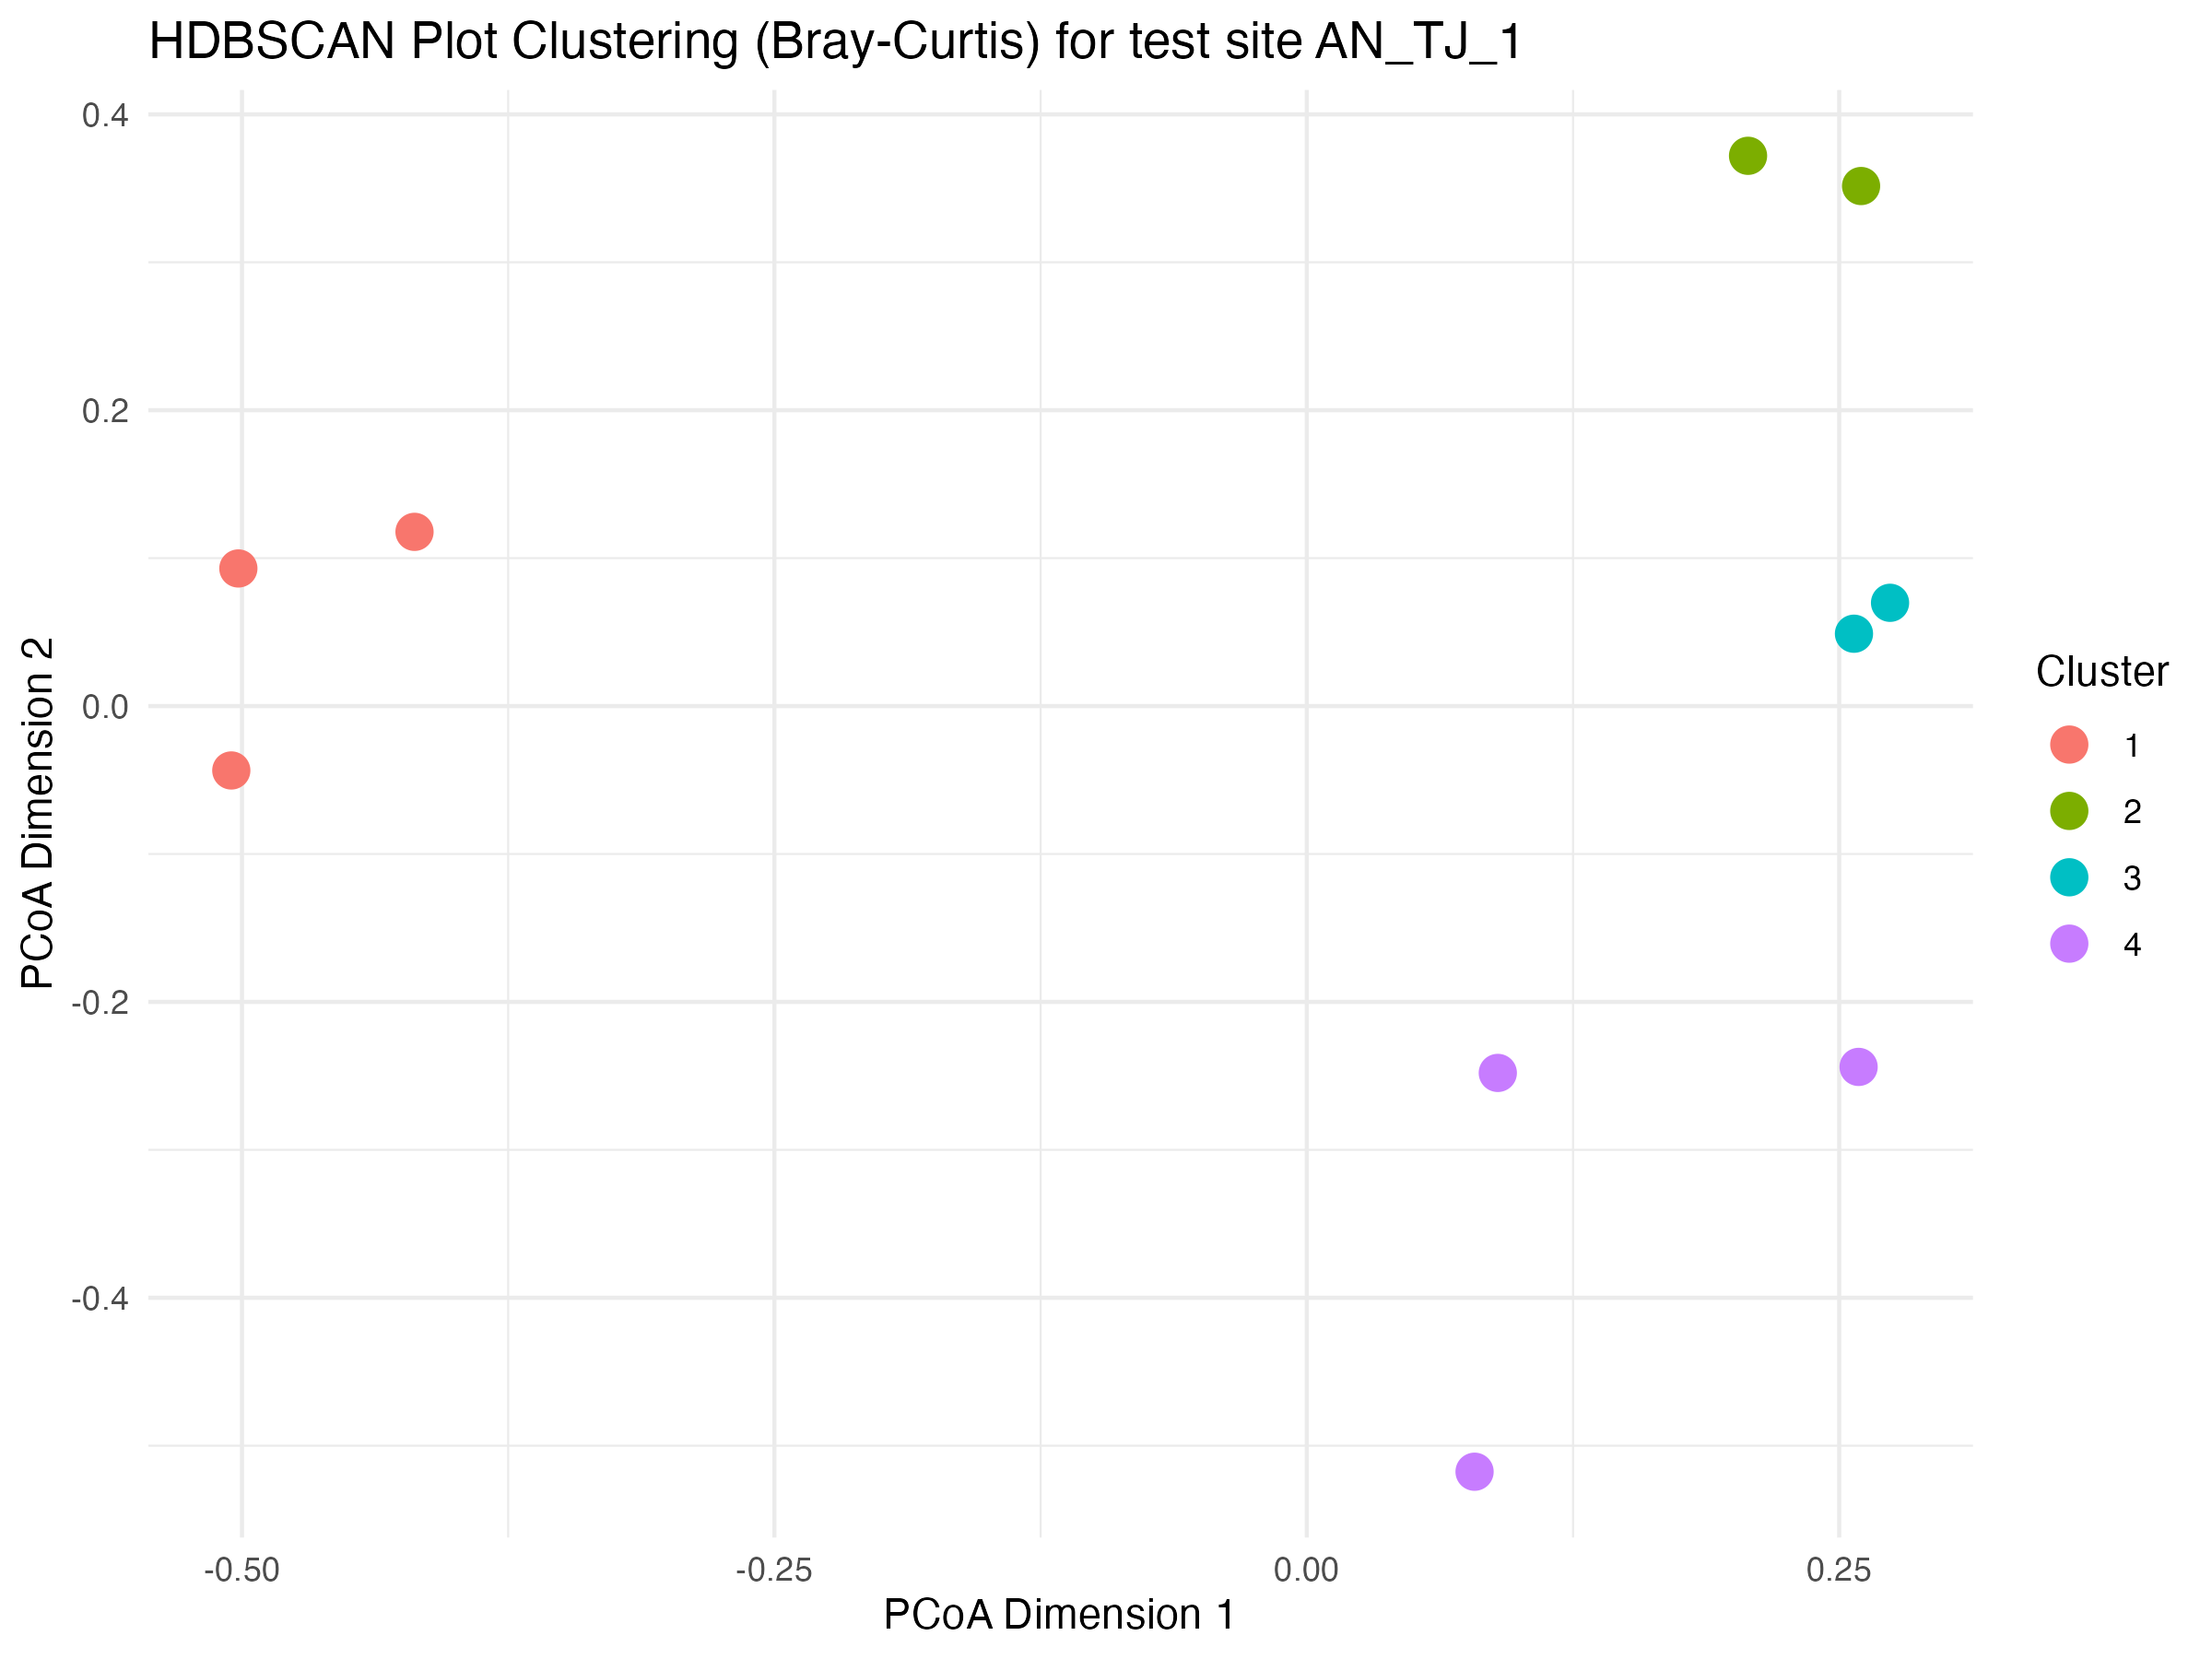
\includegraphics[width=0.9\textwidth]{Figures/Appendix/PlantCommunityClustering/AN_TJ_1_HDBSCAN_clusters.png} % Replace with your actual image path
    \caption{Community cluster HDBSCAN plot for test site AN\_TJ\_1}
    \label{fig:AN_TJ_1_HDBSCAN_clusters}
\end{figure}

\begin{figure}[H]
    \centering
    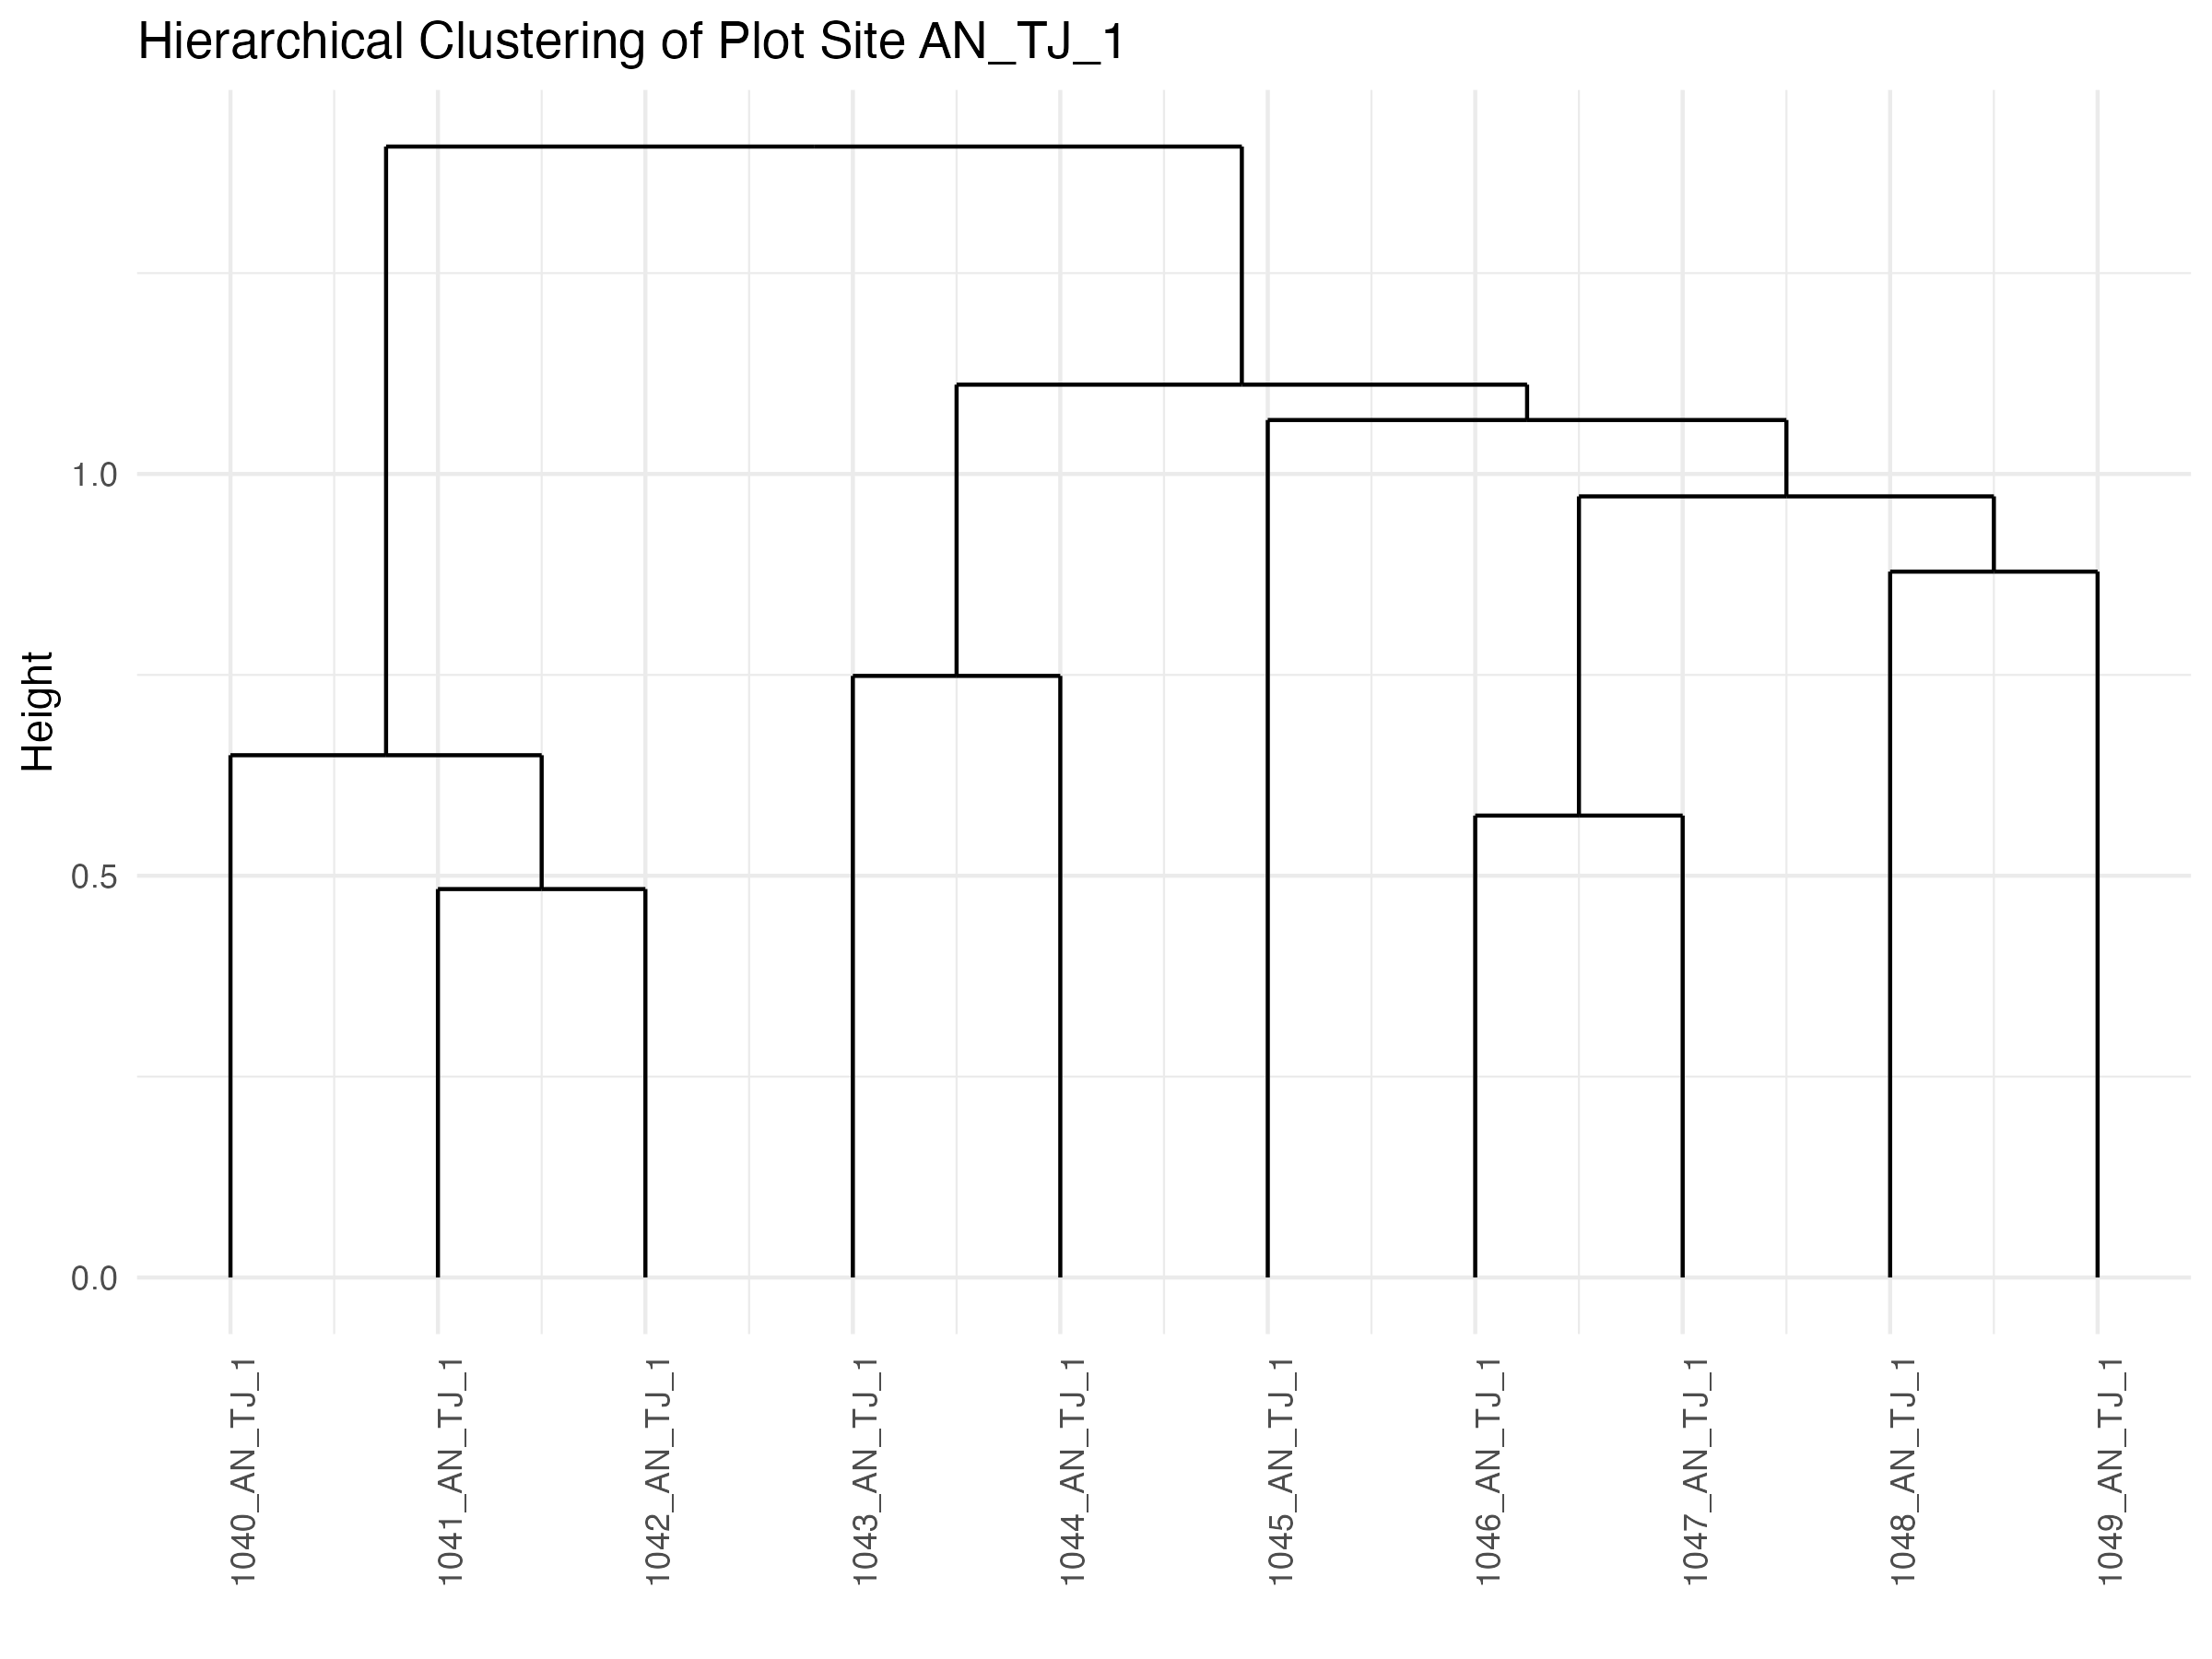
\includegraphics[width=0.9\textwidth]{Figures/Appendix/PlantCommunityClustering/AN_TJ_1_DENDRO.png} % Replace with your actual image path
    \caption{Community cluster dendrogram plot for test site AN\_TJ\_1}
    \label{fig:AN_TJ_1_DENDRO}
\end{figure}

\newpage

\subsection{AN\_TJ\_2}
\begin{figure}[H]
    \centering
    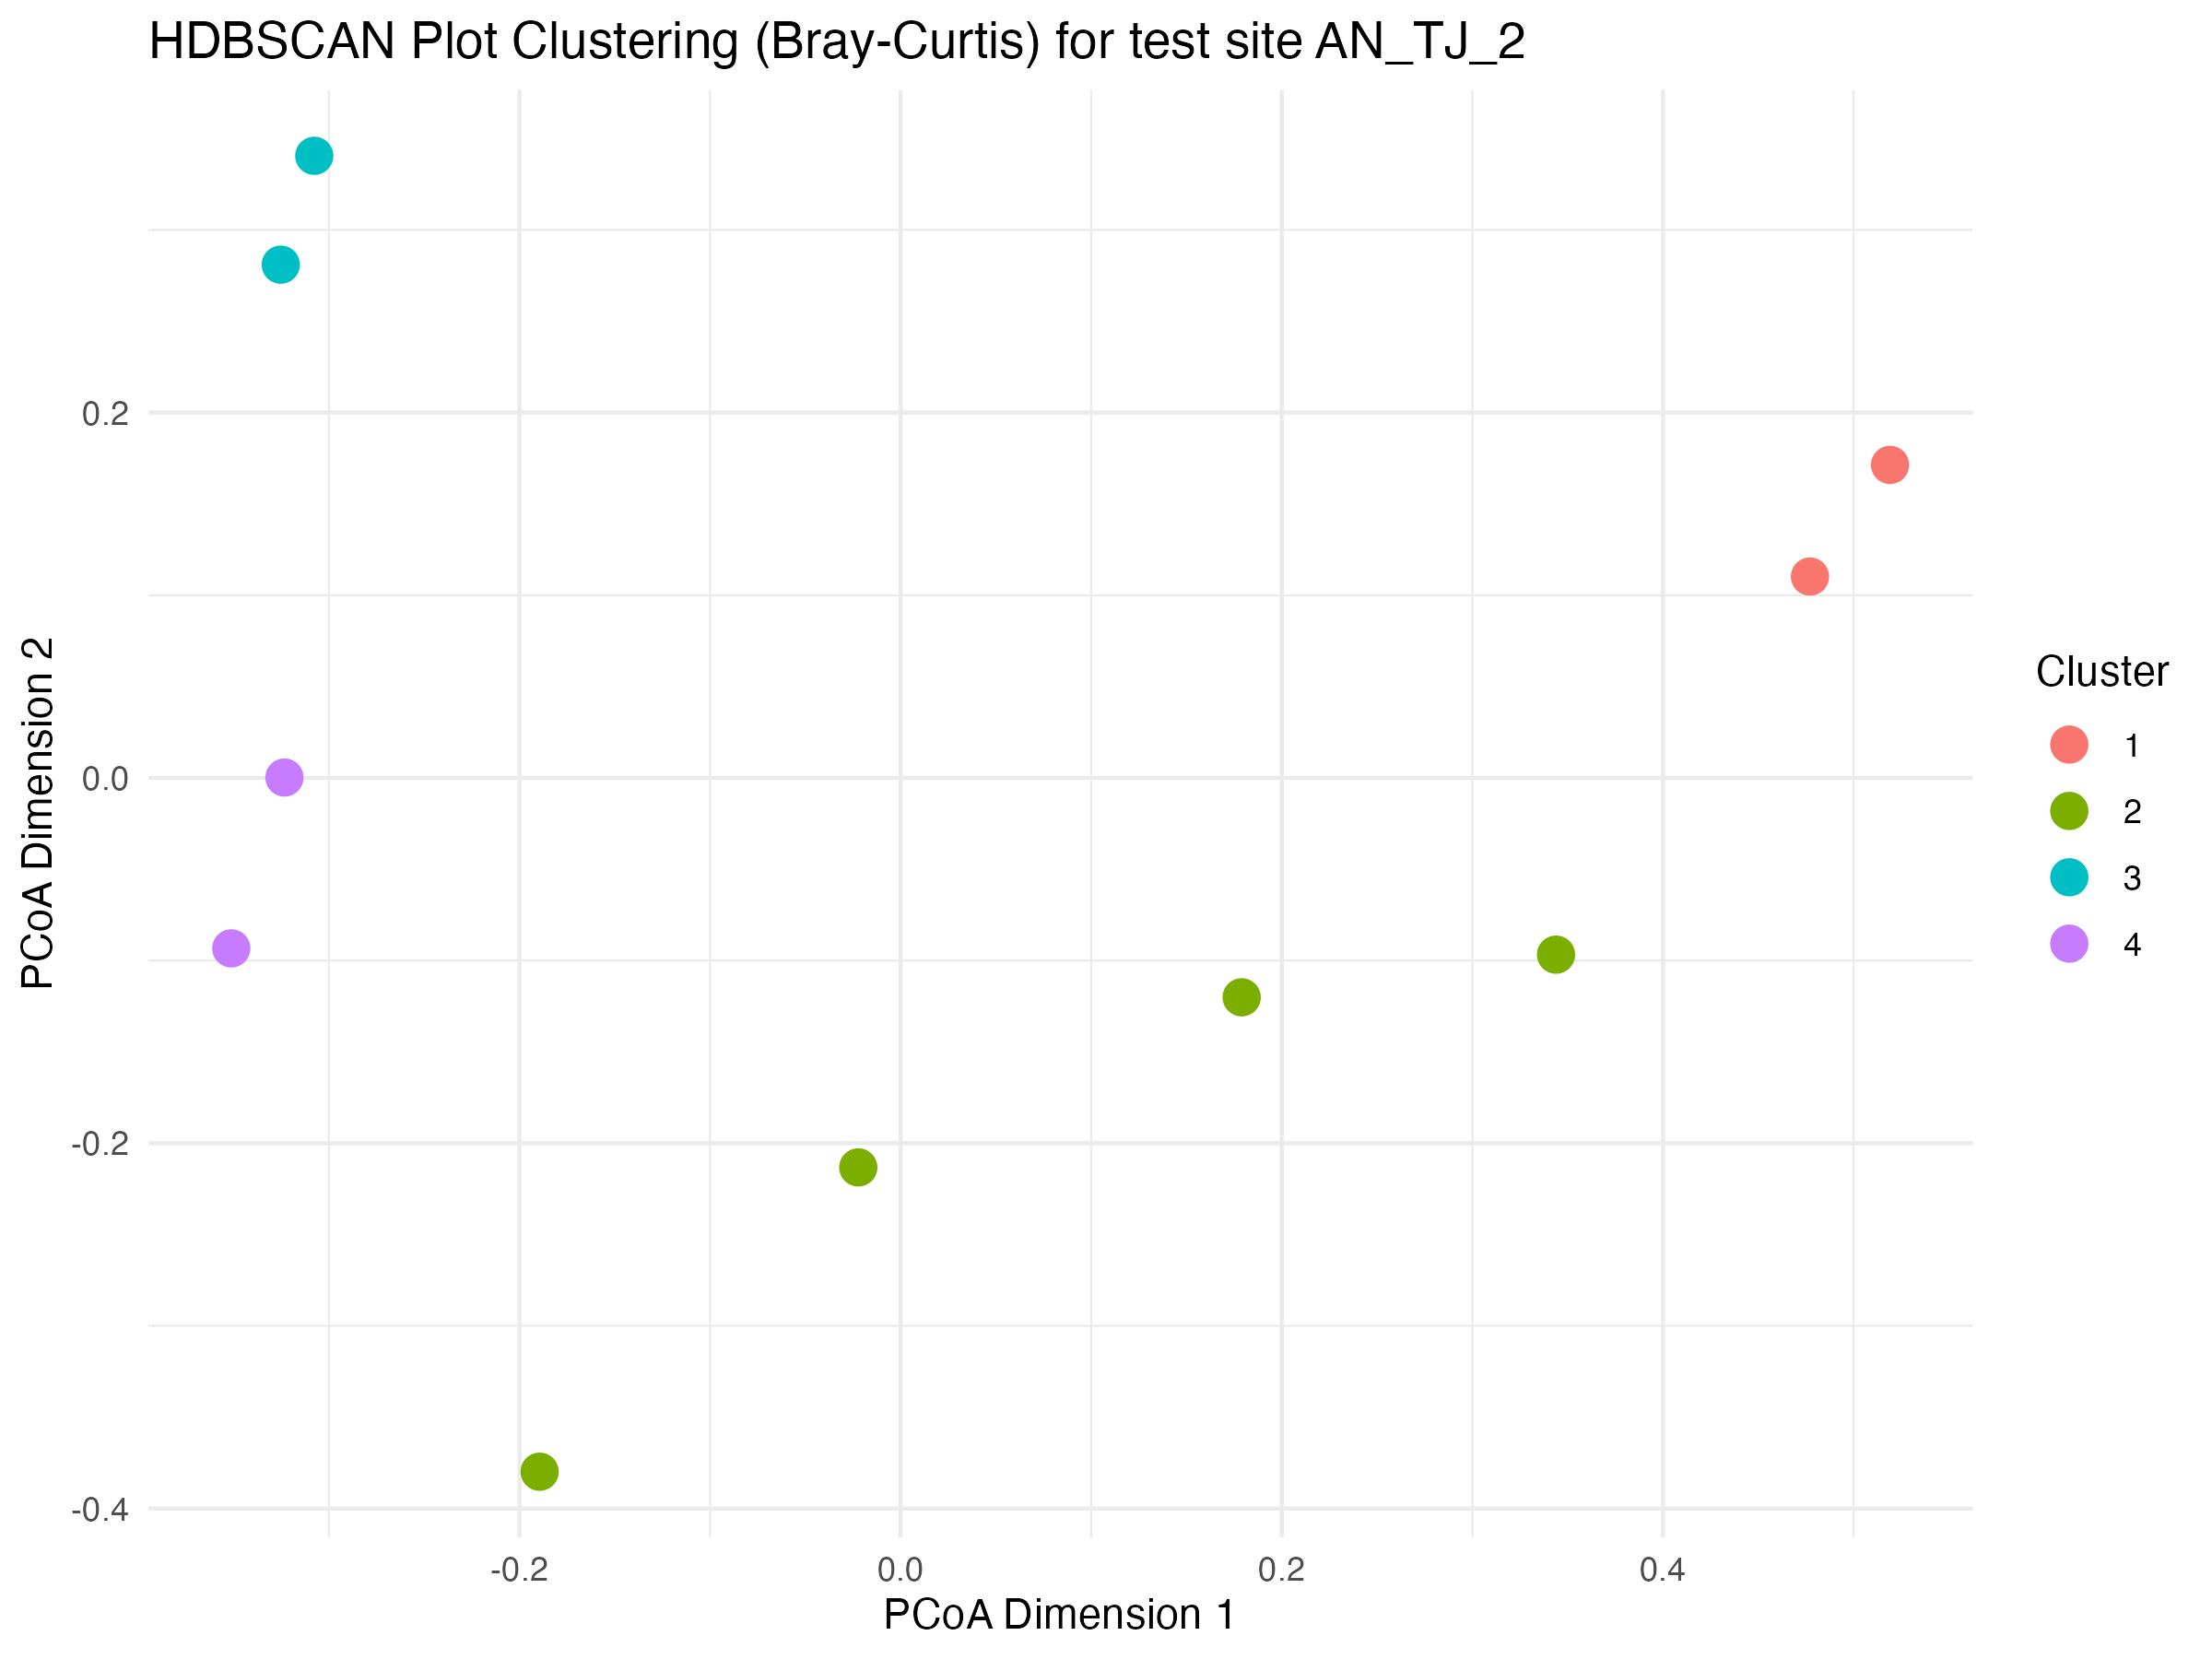
\includegraphics[width=0.9\textwidth]{Figures/Appendix/PlantCommunityClustering/AN_TJ_2_HDBSCAN_clusters.png} % Replace with your actual image path
    \caption{Community cluster HDBSCAN plot for test site AN\_TJ\_2}
    \label{fig:AN_TJ_2_HDBSCAN_clusters}
\end{figure}

\begin{figure}[H]
    \centering
    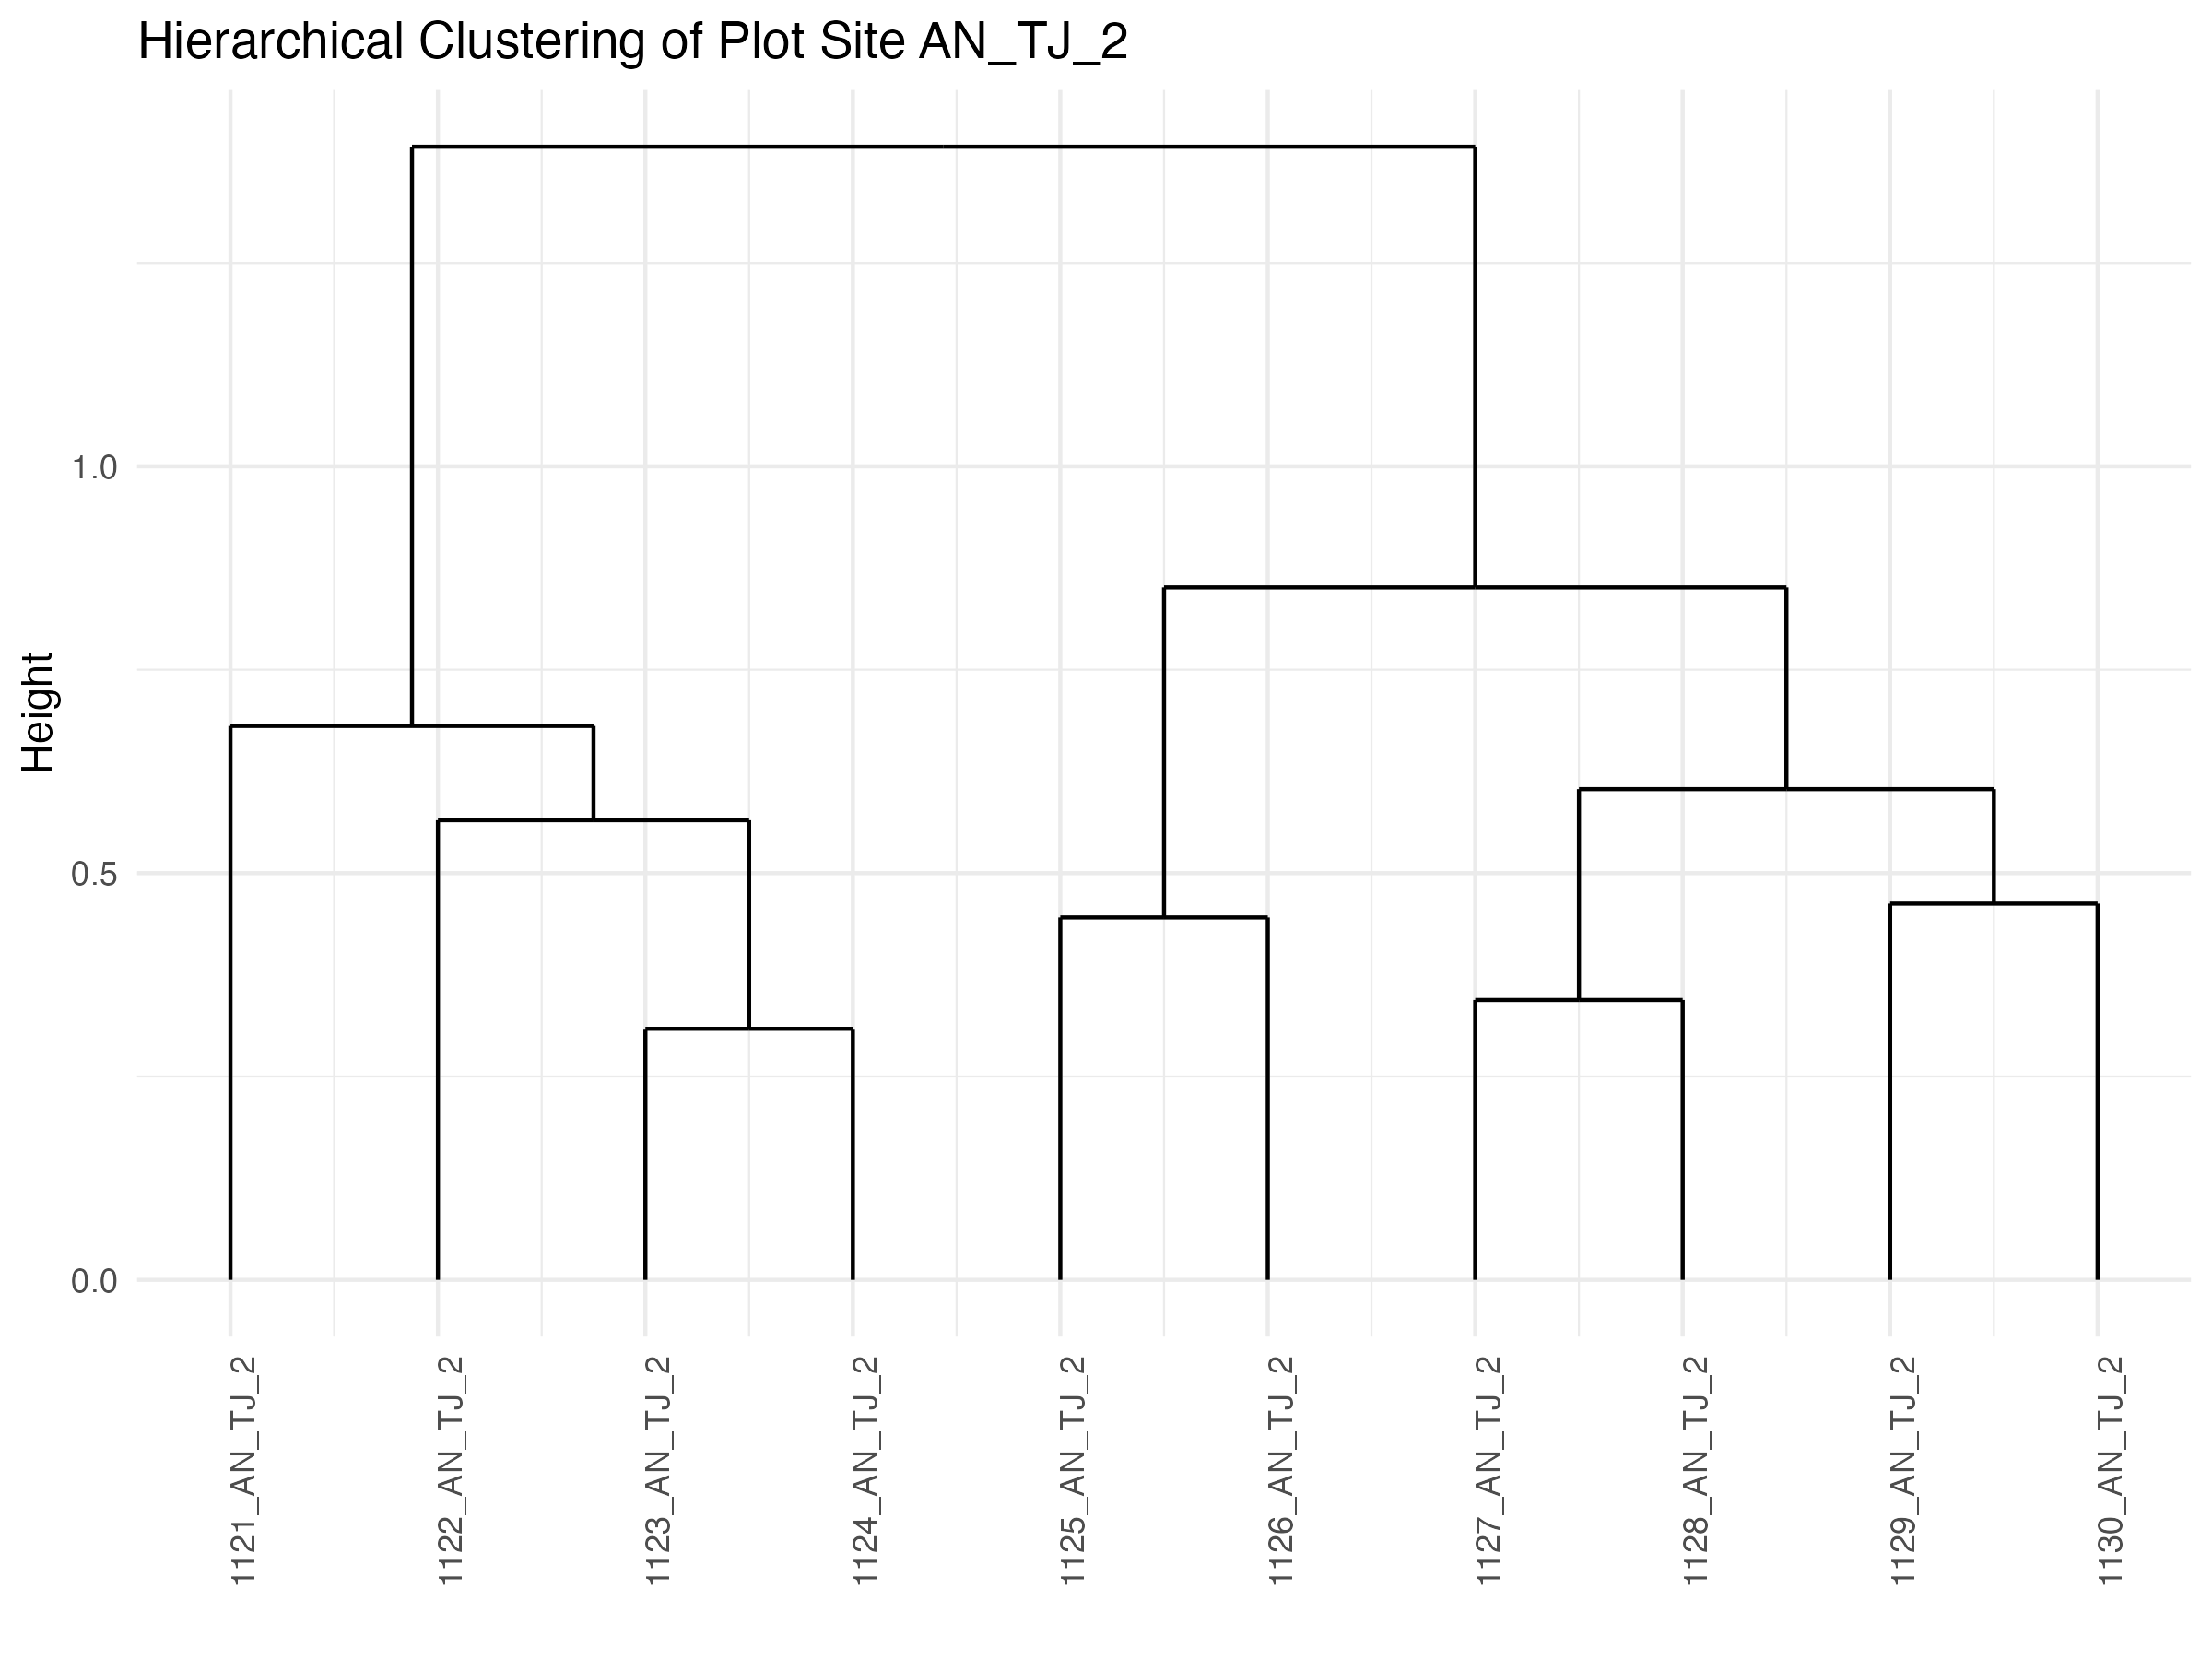
\includegraphics[width=0.9\textwidth]{Figures/Appendix/PlantCommunityClustering/AN_TJ_2_DENDRO.png} % Replace with your actual image path
    \caption{Community cluster dendrogram plot for test site AN\_TJ\_2}
    \label{fig:AN_TJ_2_DENDRO}
\end{figure}

\subsection{ATQ\_VK\_1}
\begin{figure}[H]
    \centering
    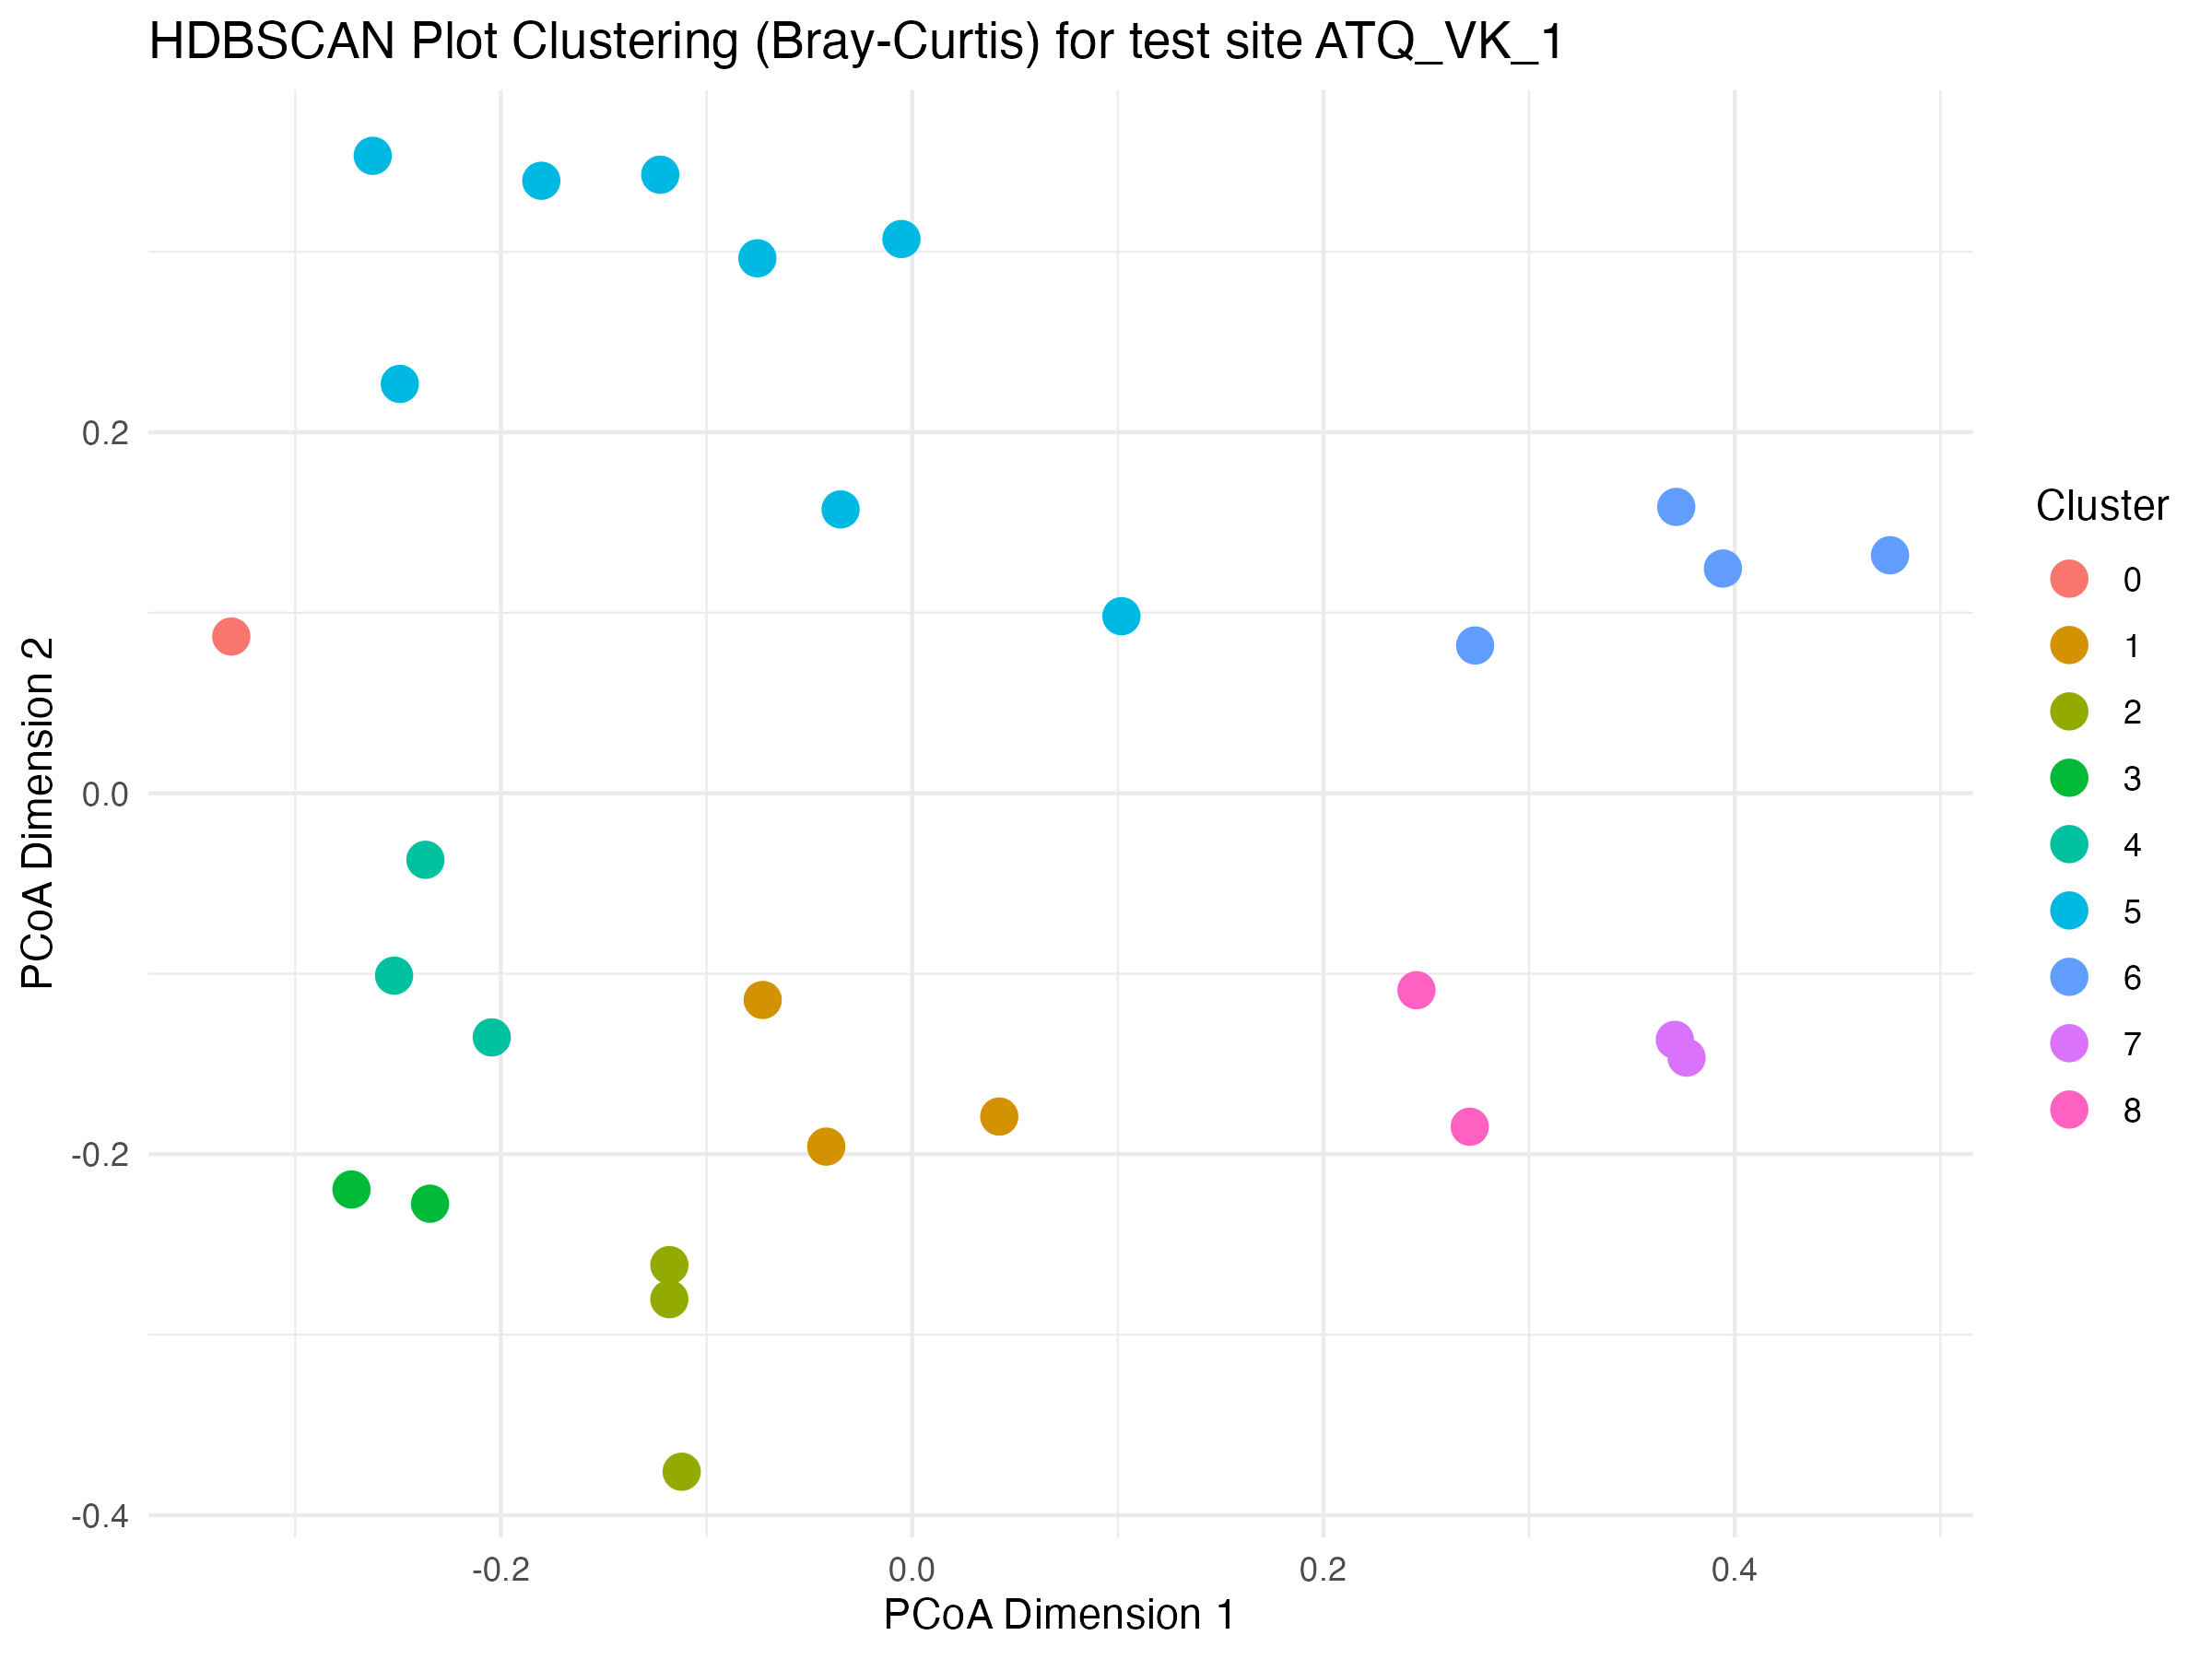
\includegraphics[width=0.9\textwidth]{Figures/Appendix/PlantCommunityClustering/ATQ_VK_1_HDBSCAN_clusters.png} % Replace with your actual image path
    \caption{Community cluster HDBSCAN plot for test site ATQ\_VK\_1}
    \label{fig:ATQ_VK_1_HDBSCAN_clusters}
\end{figure}

\begin{figure}[H]
    \centering
    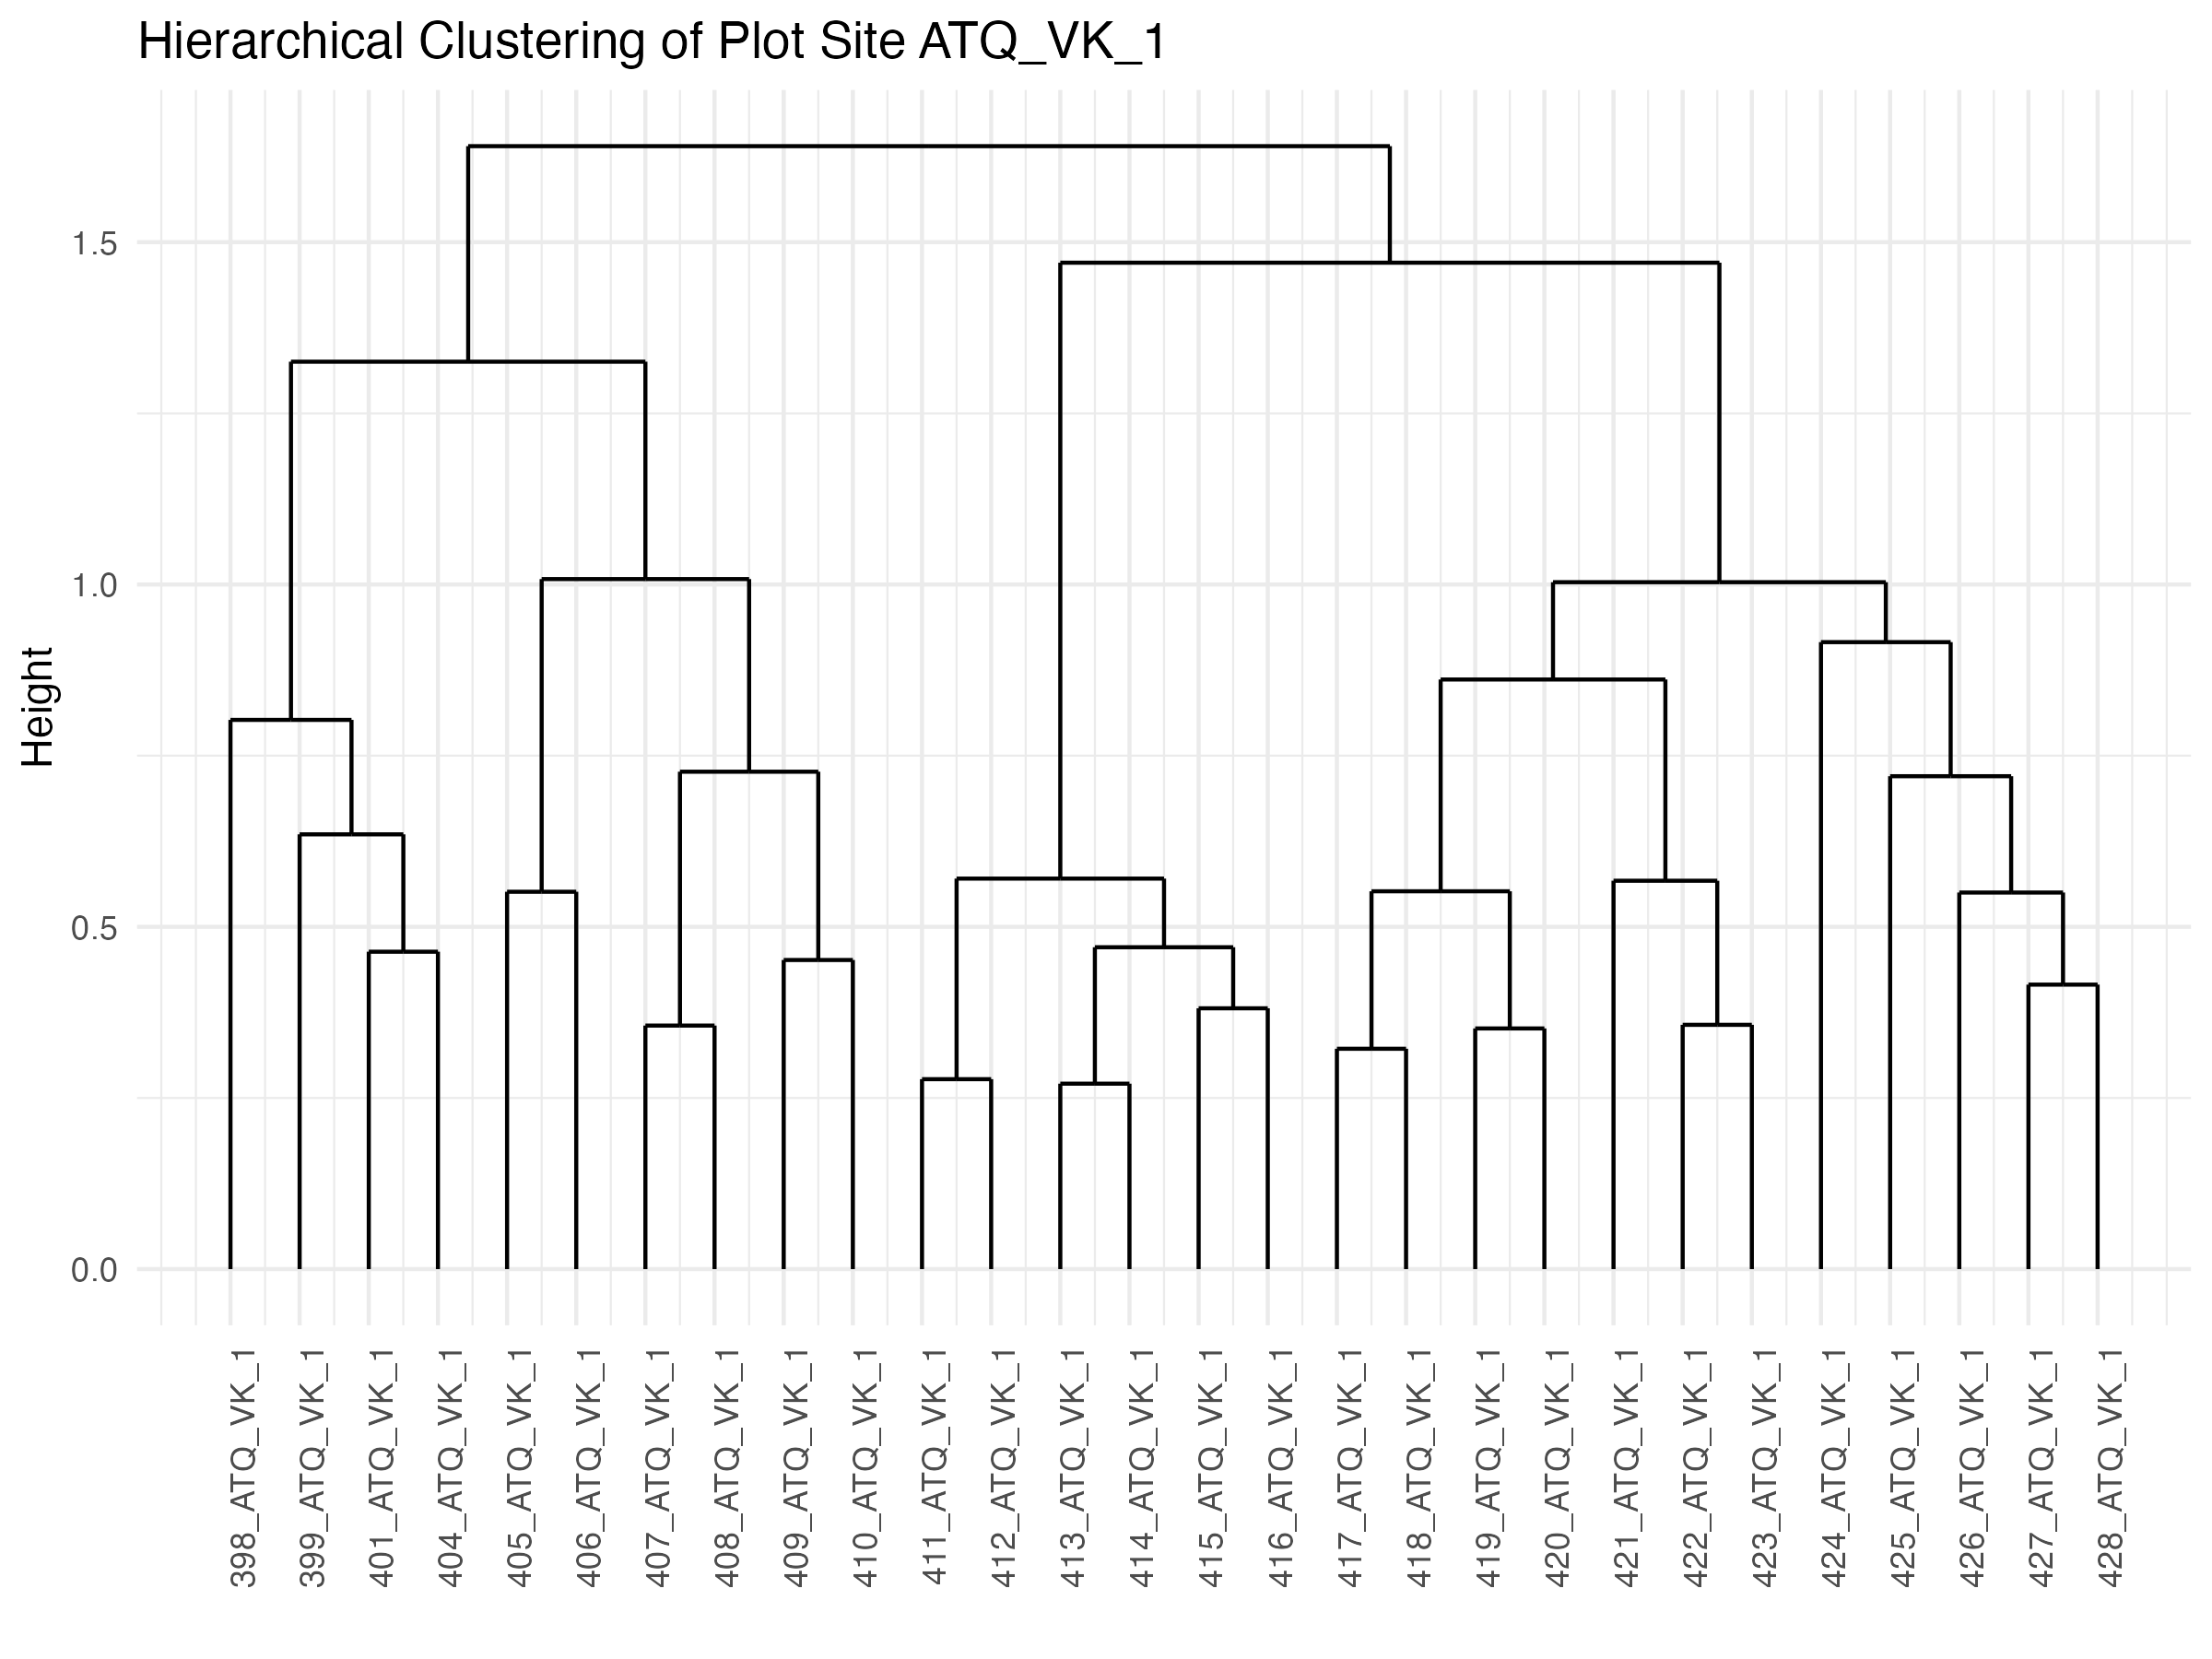
\includegraphics[width=0.9\textwidth]{Figures/Appendix/PlantCommunityClustering/ATQ_VK_1_DENDRO.png} % Replace with your actual image path
    \caption{Community cluster dendrogram plot for test site ATQ\_VK\_1}
    \label{fig:ATQ_VK_1_DENDRO}
\end{figure}

\subsection{BRW\_PW\_1}
\begin{figure}[H]
    \centering
    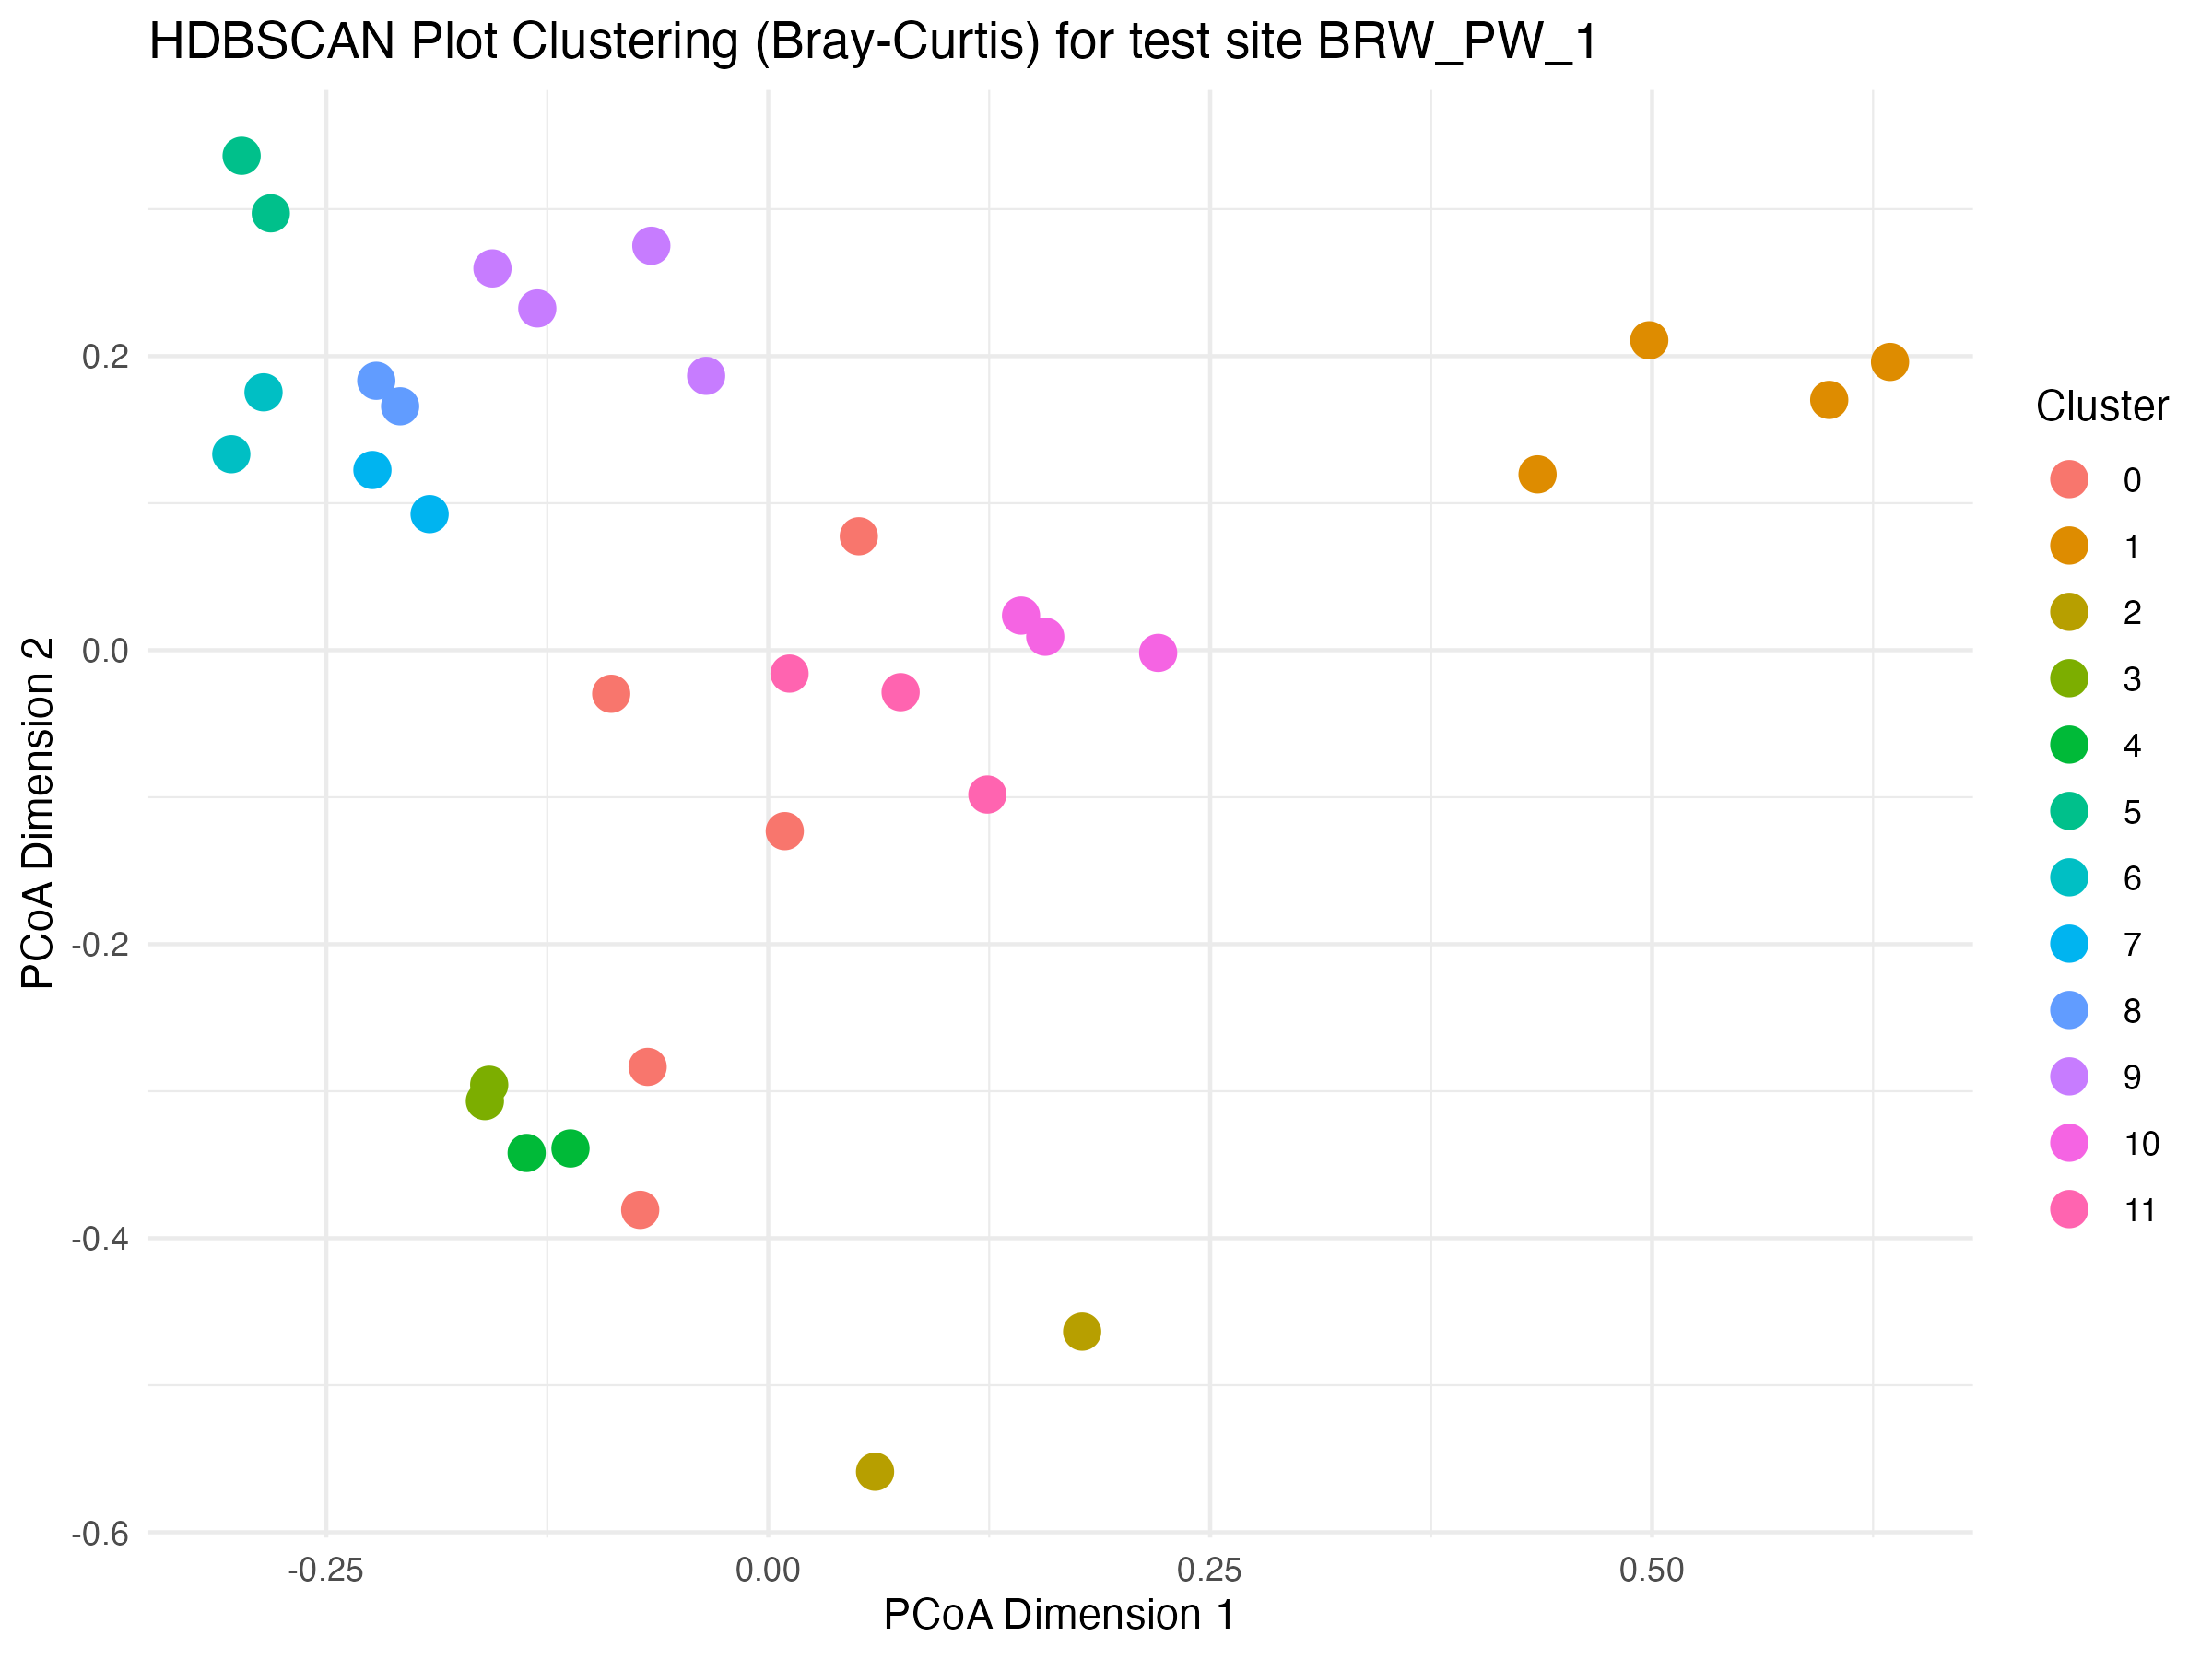
\includegraphics[width=0.9\textwidth]{Figures/Appendix/PlantCommunityClustering/BRW_PW_1_HDBSCAN_clusters.png} % Replace with your actual image path
    \caption{Community cluster HDBSCAN plot for test site BRW\_PW\_1}
    \label{fig:BRW_PW_1_HDBSCAN_clusters}
\end{figure}

\begin{figure}[H]
    \centering
    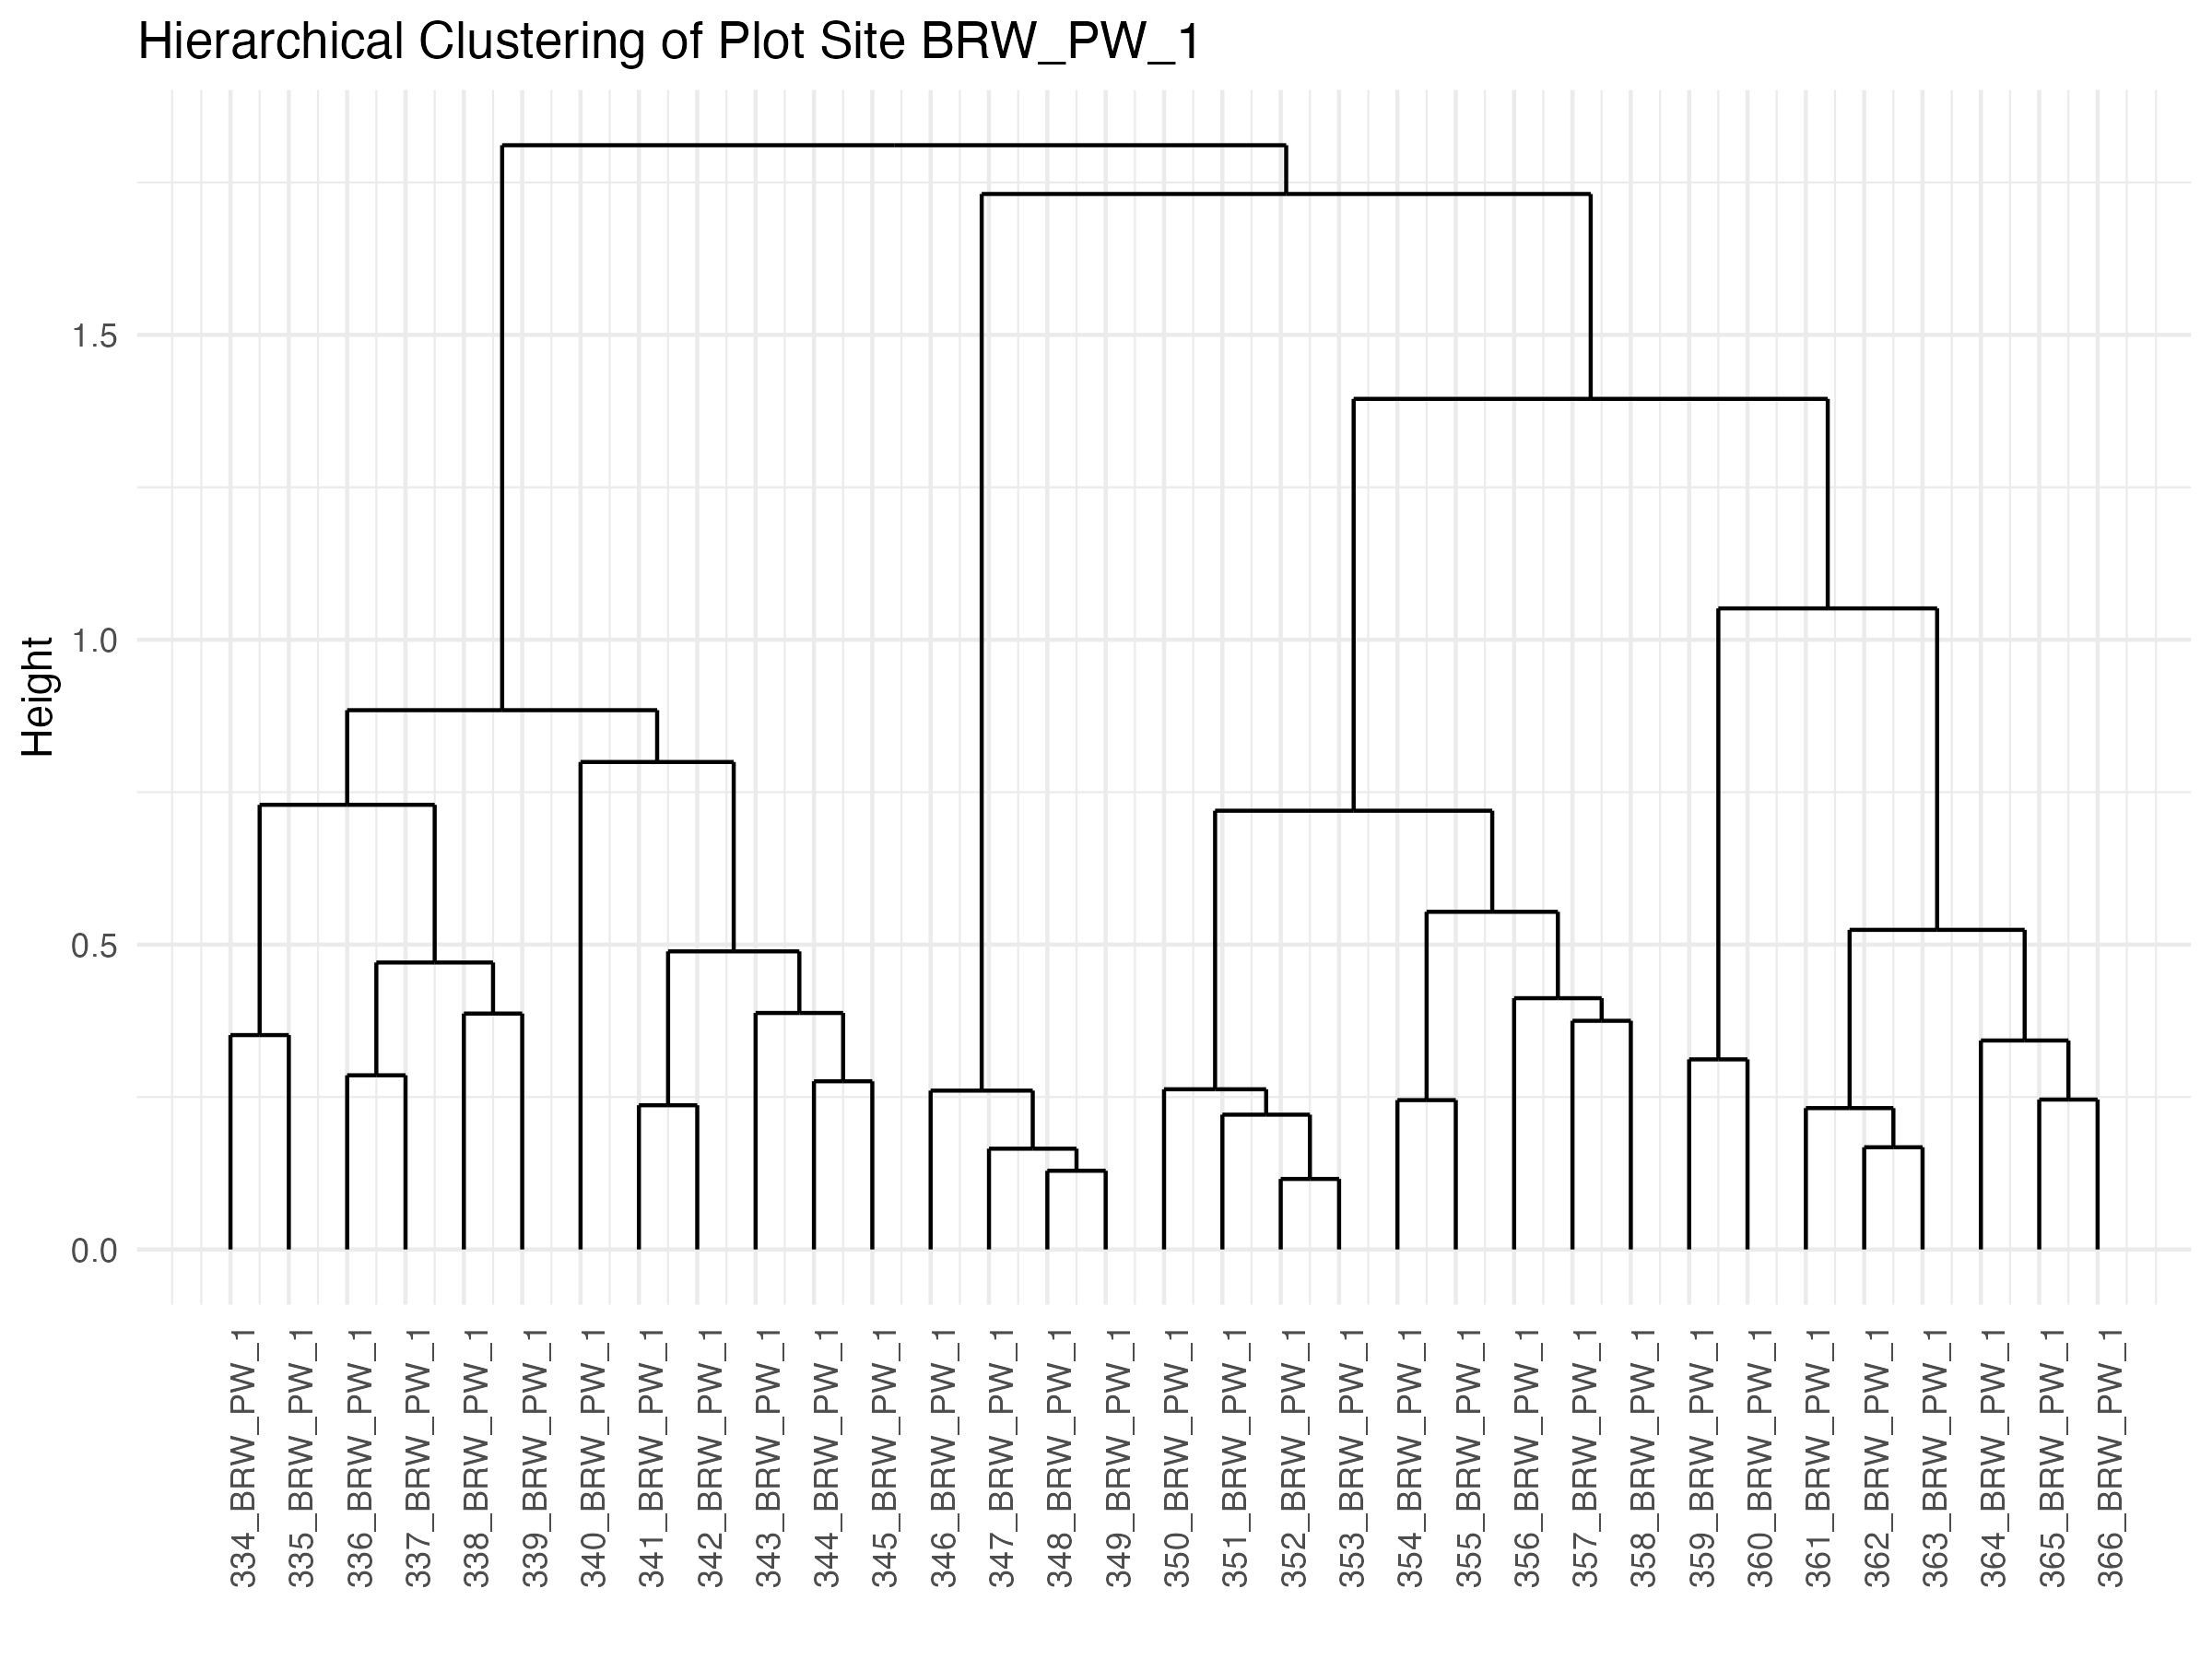
\includegraphics[width=0.9\textwidth]{Figures/Appendix/PlantCommunityClustering/BRW_PW_1_DENDRO.png} % Replace with your actual image path
    \caption{Community cluster dendrogram plot for test site BRW\_PW\_1}
    \label{fig:BRW_PW_1_DENDRO}
\end{figure}

\subsection{BRW\_VS\_1}
\begin{figure}[H]
    \centering
    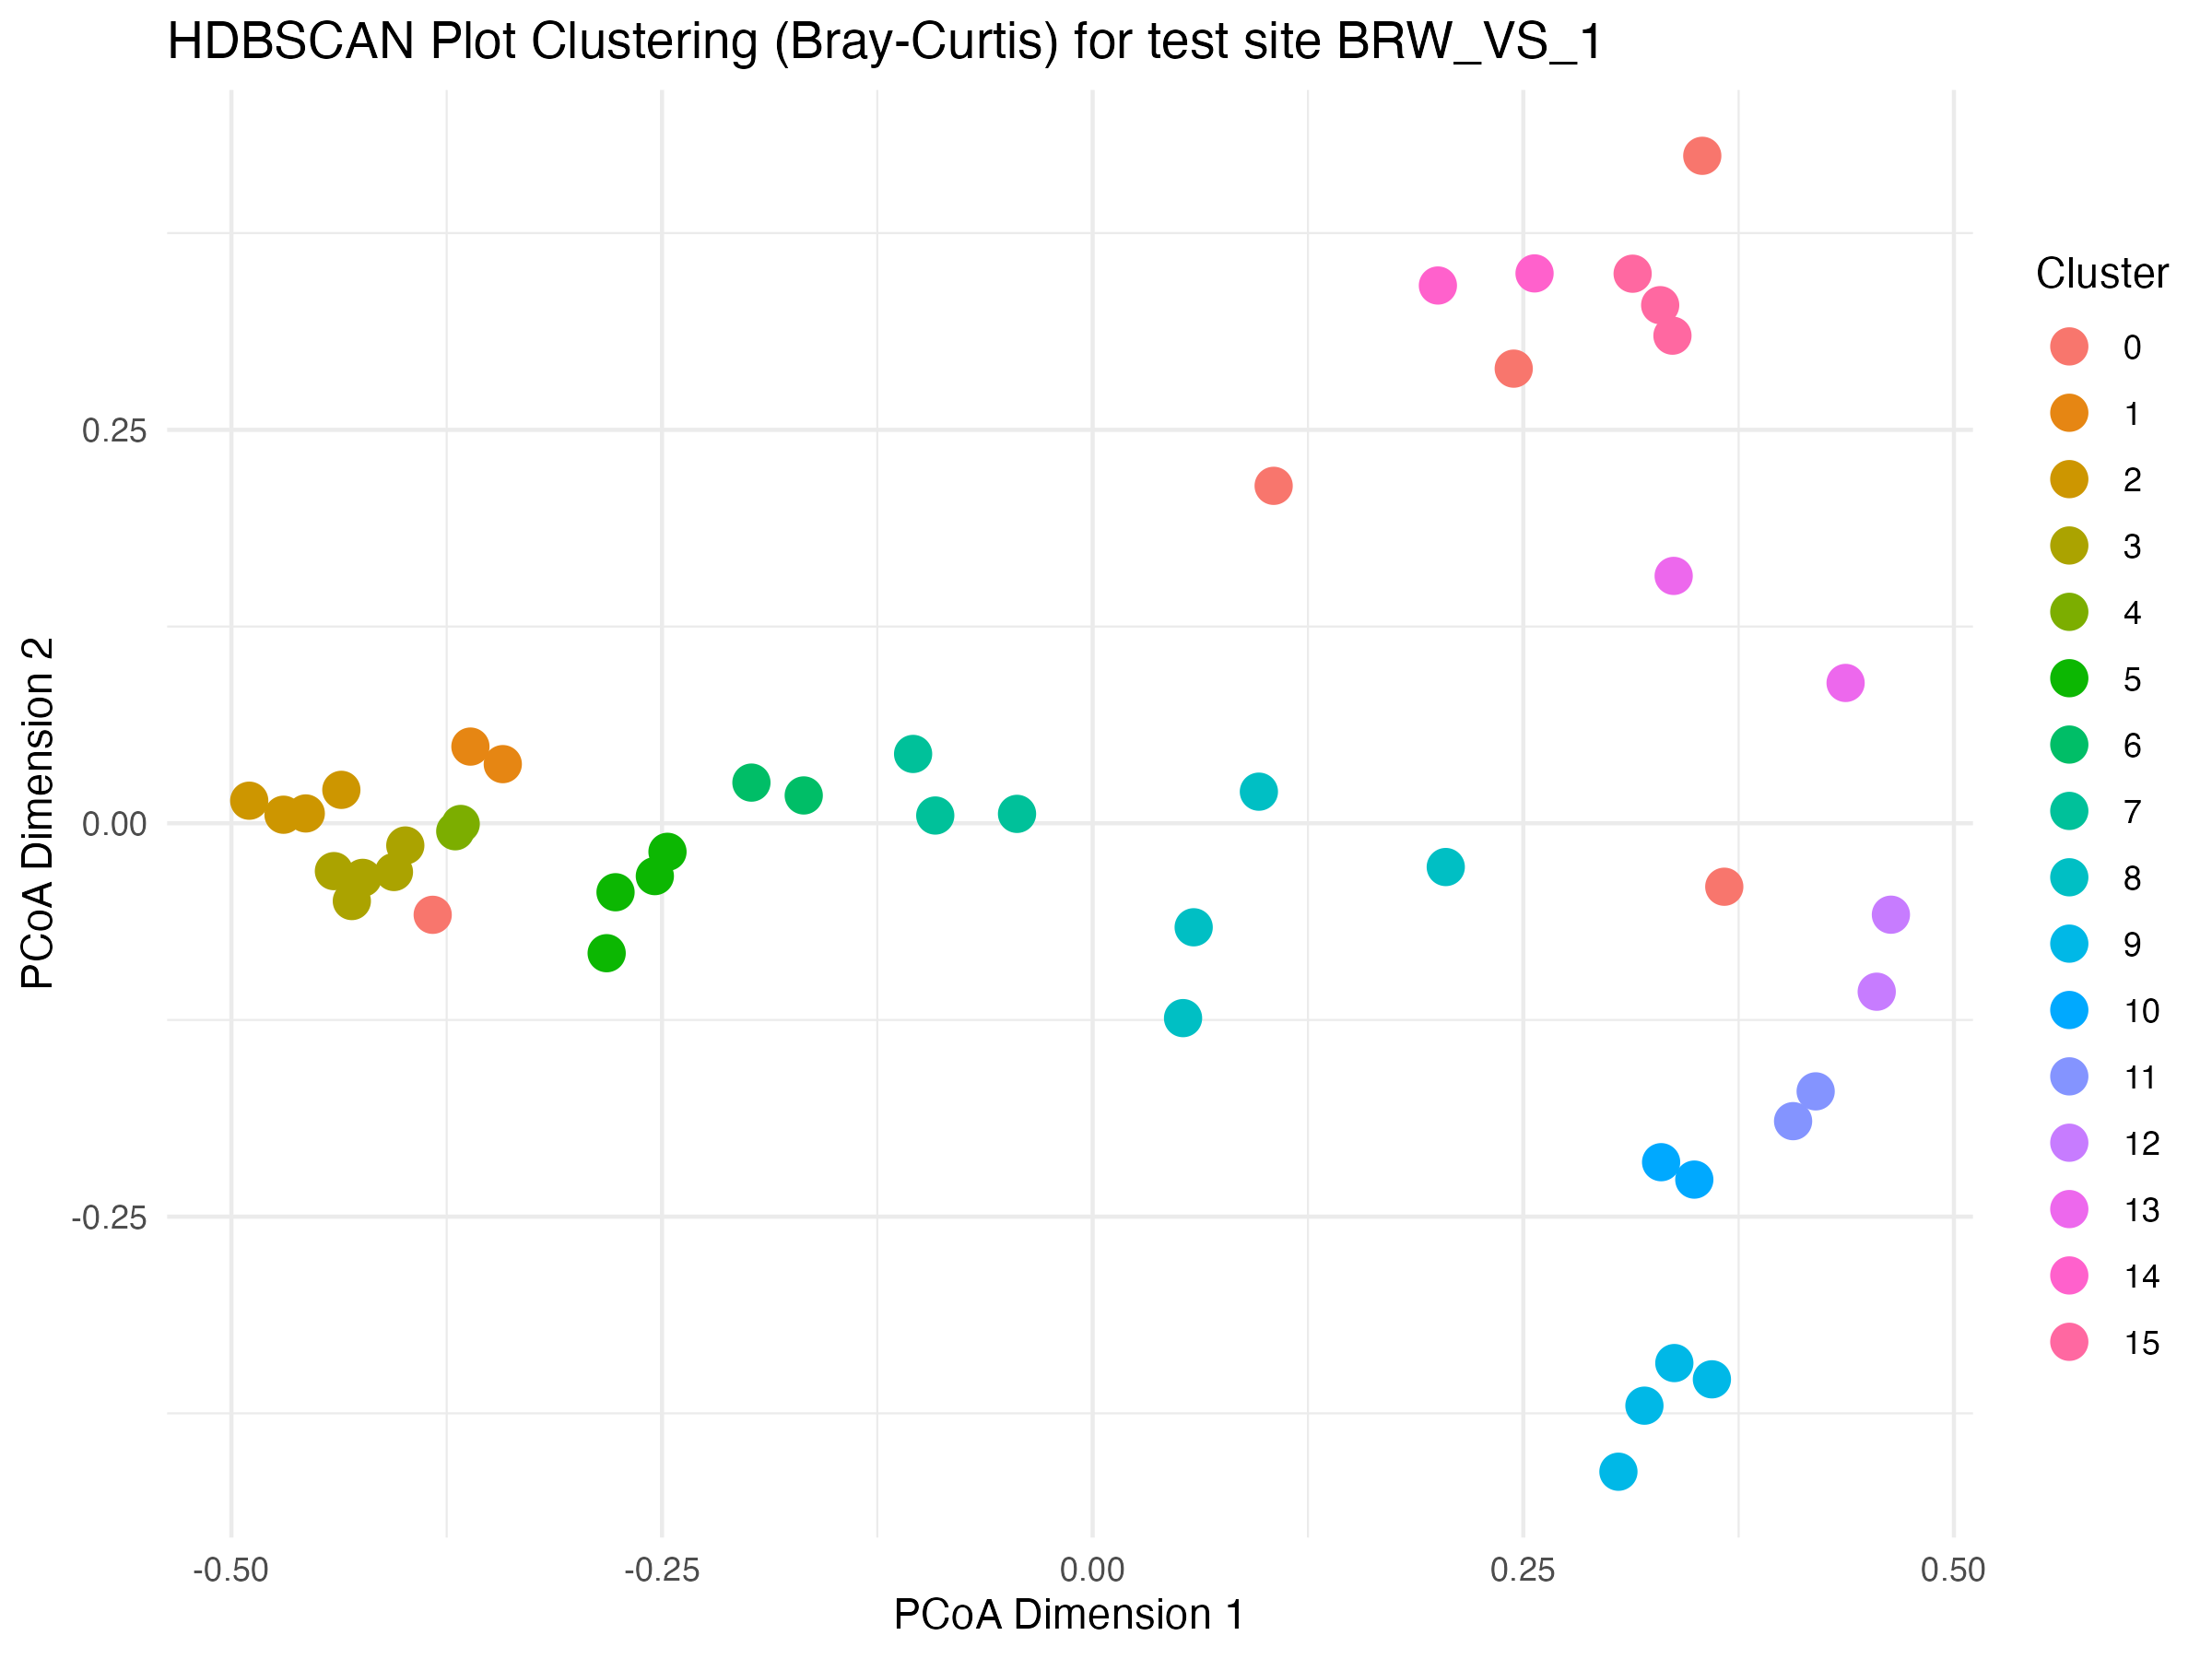
\includegraphics[width=0.9\textwidth]{Figures/Appendix/PlantCommunityClustering/BRW_VS_1_HDBSCAN_clusters.png} % Replace with your actual image path
    \caption{Community cluster HDBSCAN plot for test site BRW\_VS\_1}
    \label{fig:BRW_VS_1_HDBSCAN_clusters}
\end{figure}

\begin{figure}[H]
    \centering
    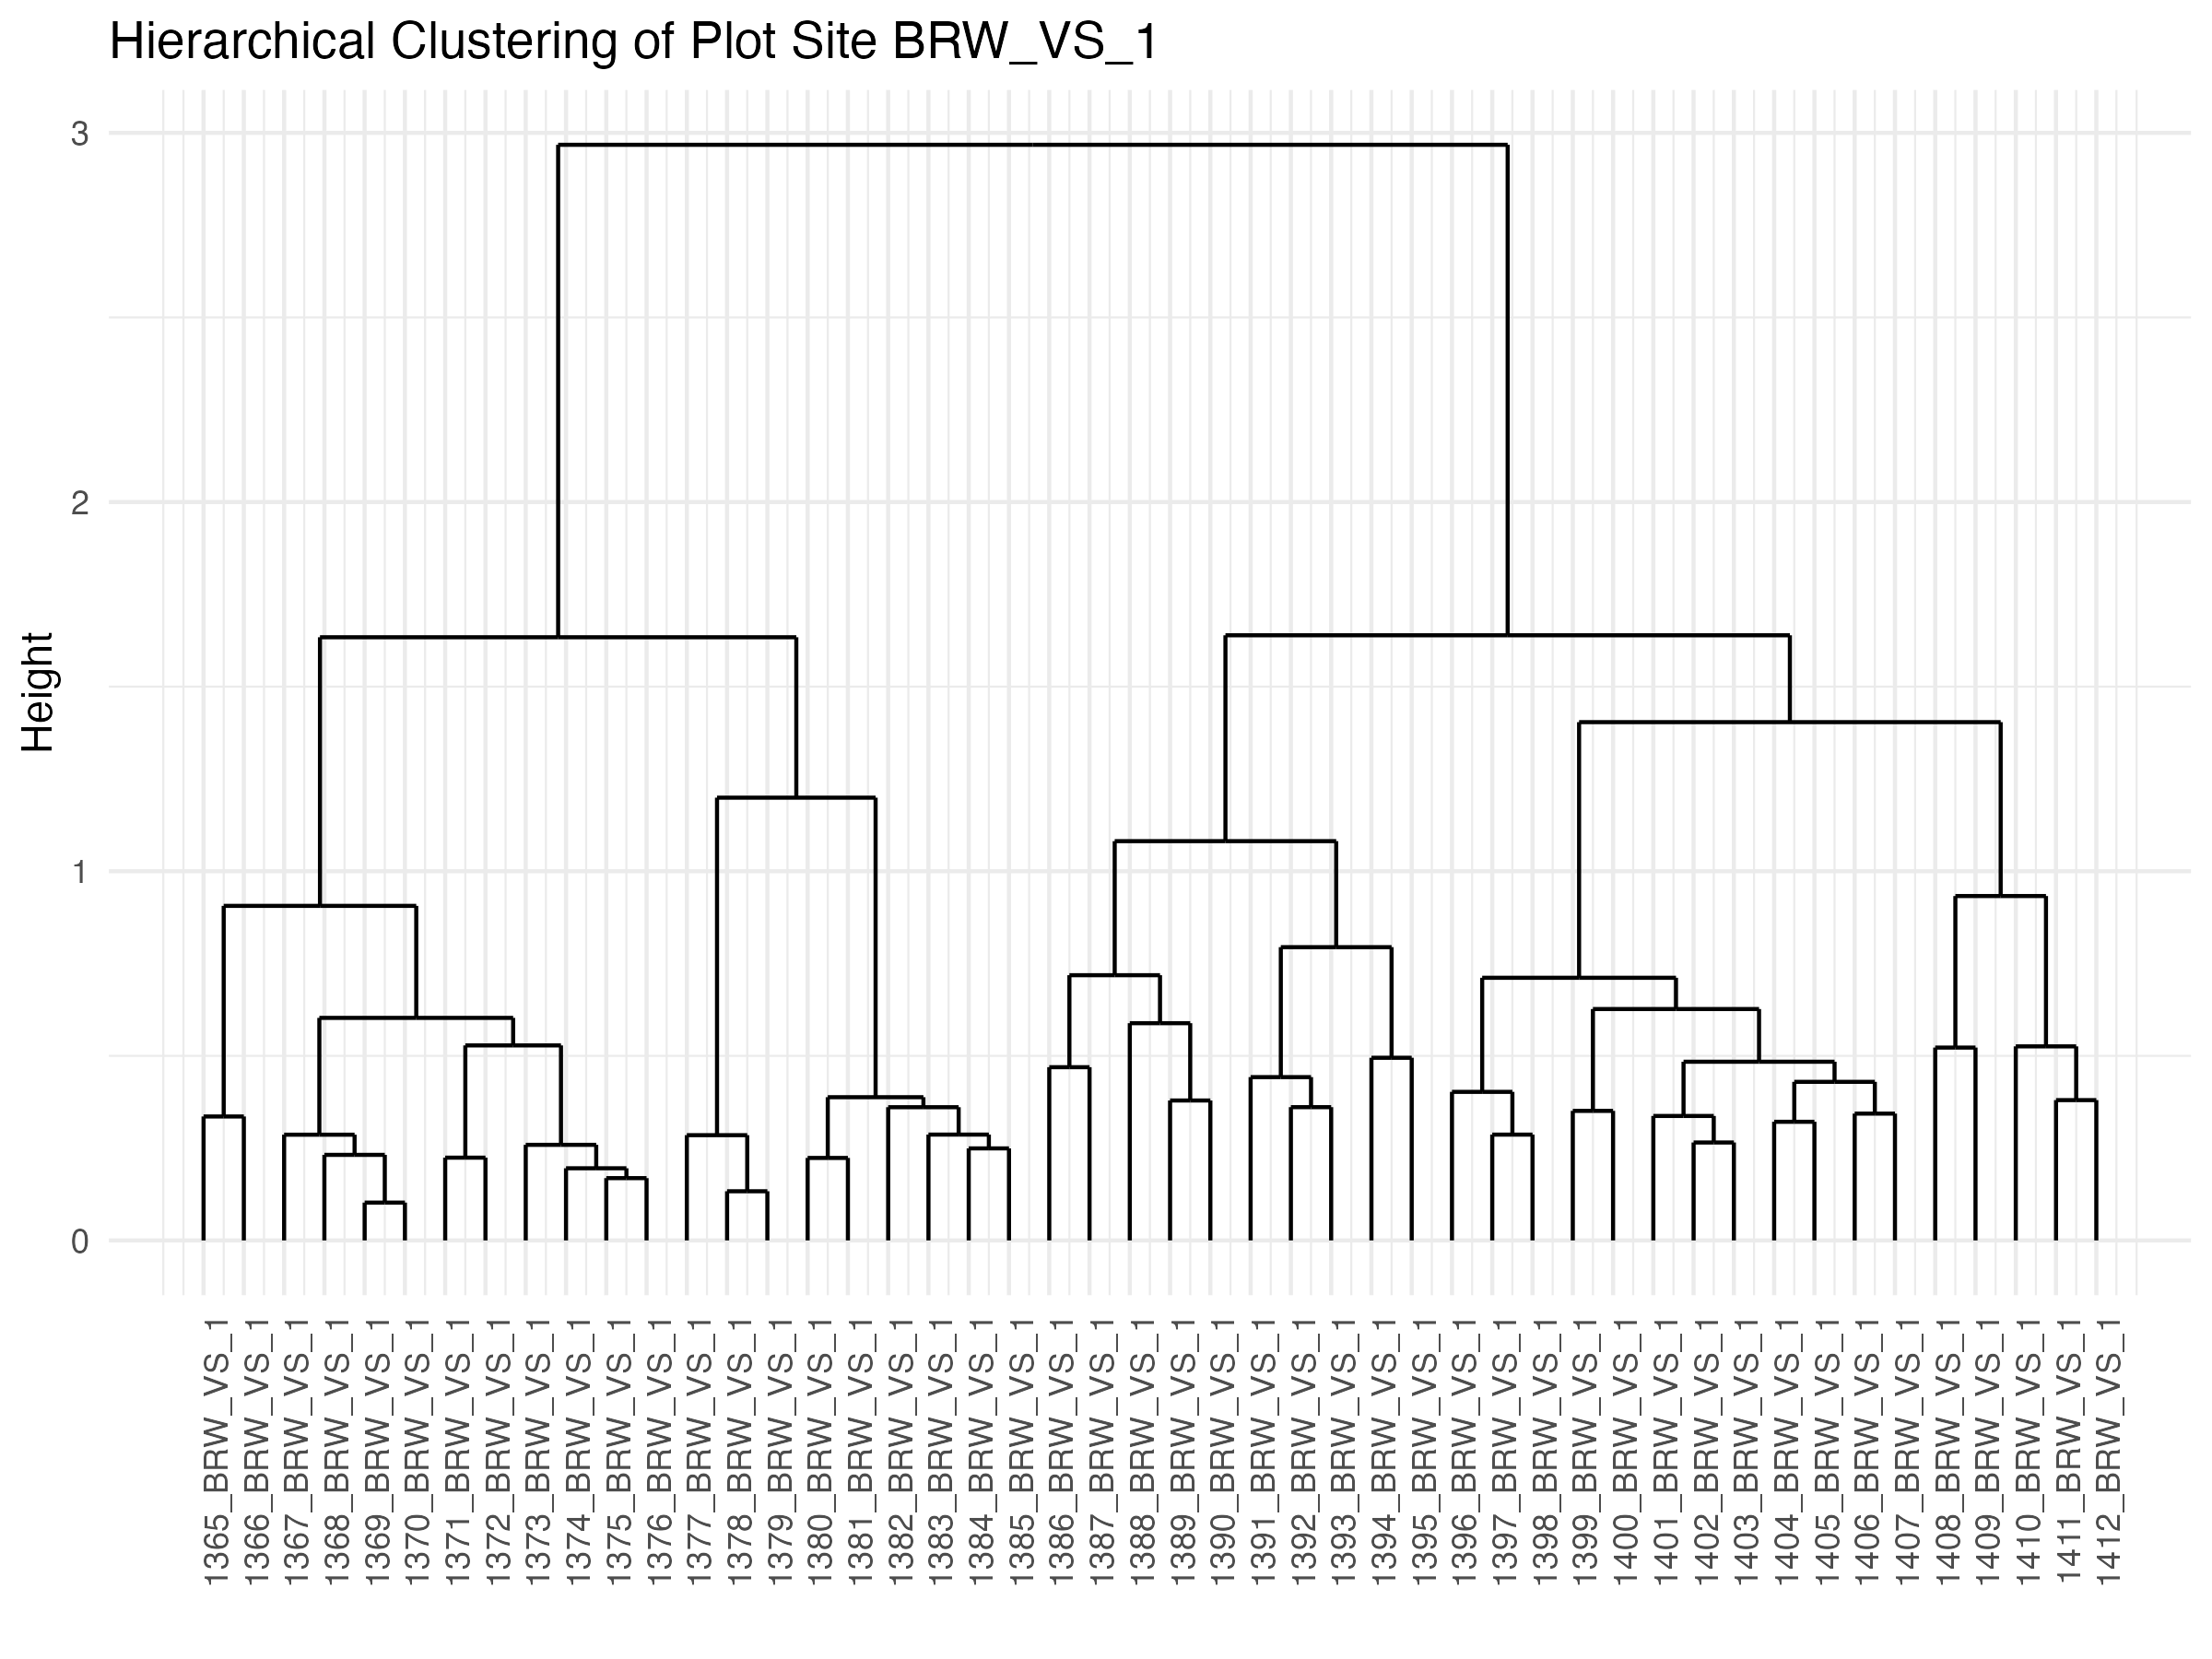
\includegraphics[width=0.9\textwidth]{Figures/Appendix/PlantCommunityClustering/BRW_VS_1_DENDRO.png} % Replace with your actual image path
    \caption{Community cluster dendrogram plot for test site BRW\_VS\_1}
    \label{fig:BRW_VS_1_DENDRO}
\end{figure}

\subsection{FLXTWRZONA\_SD\_1}
\begin{figure}[H]
    \centering
    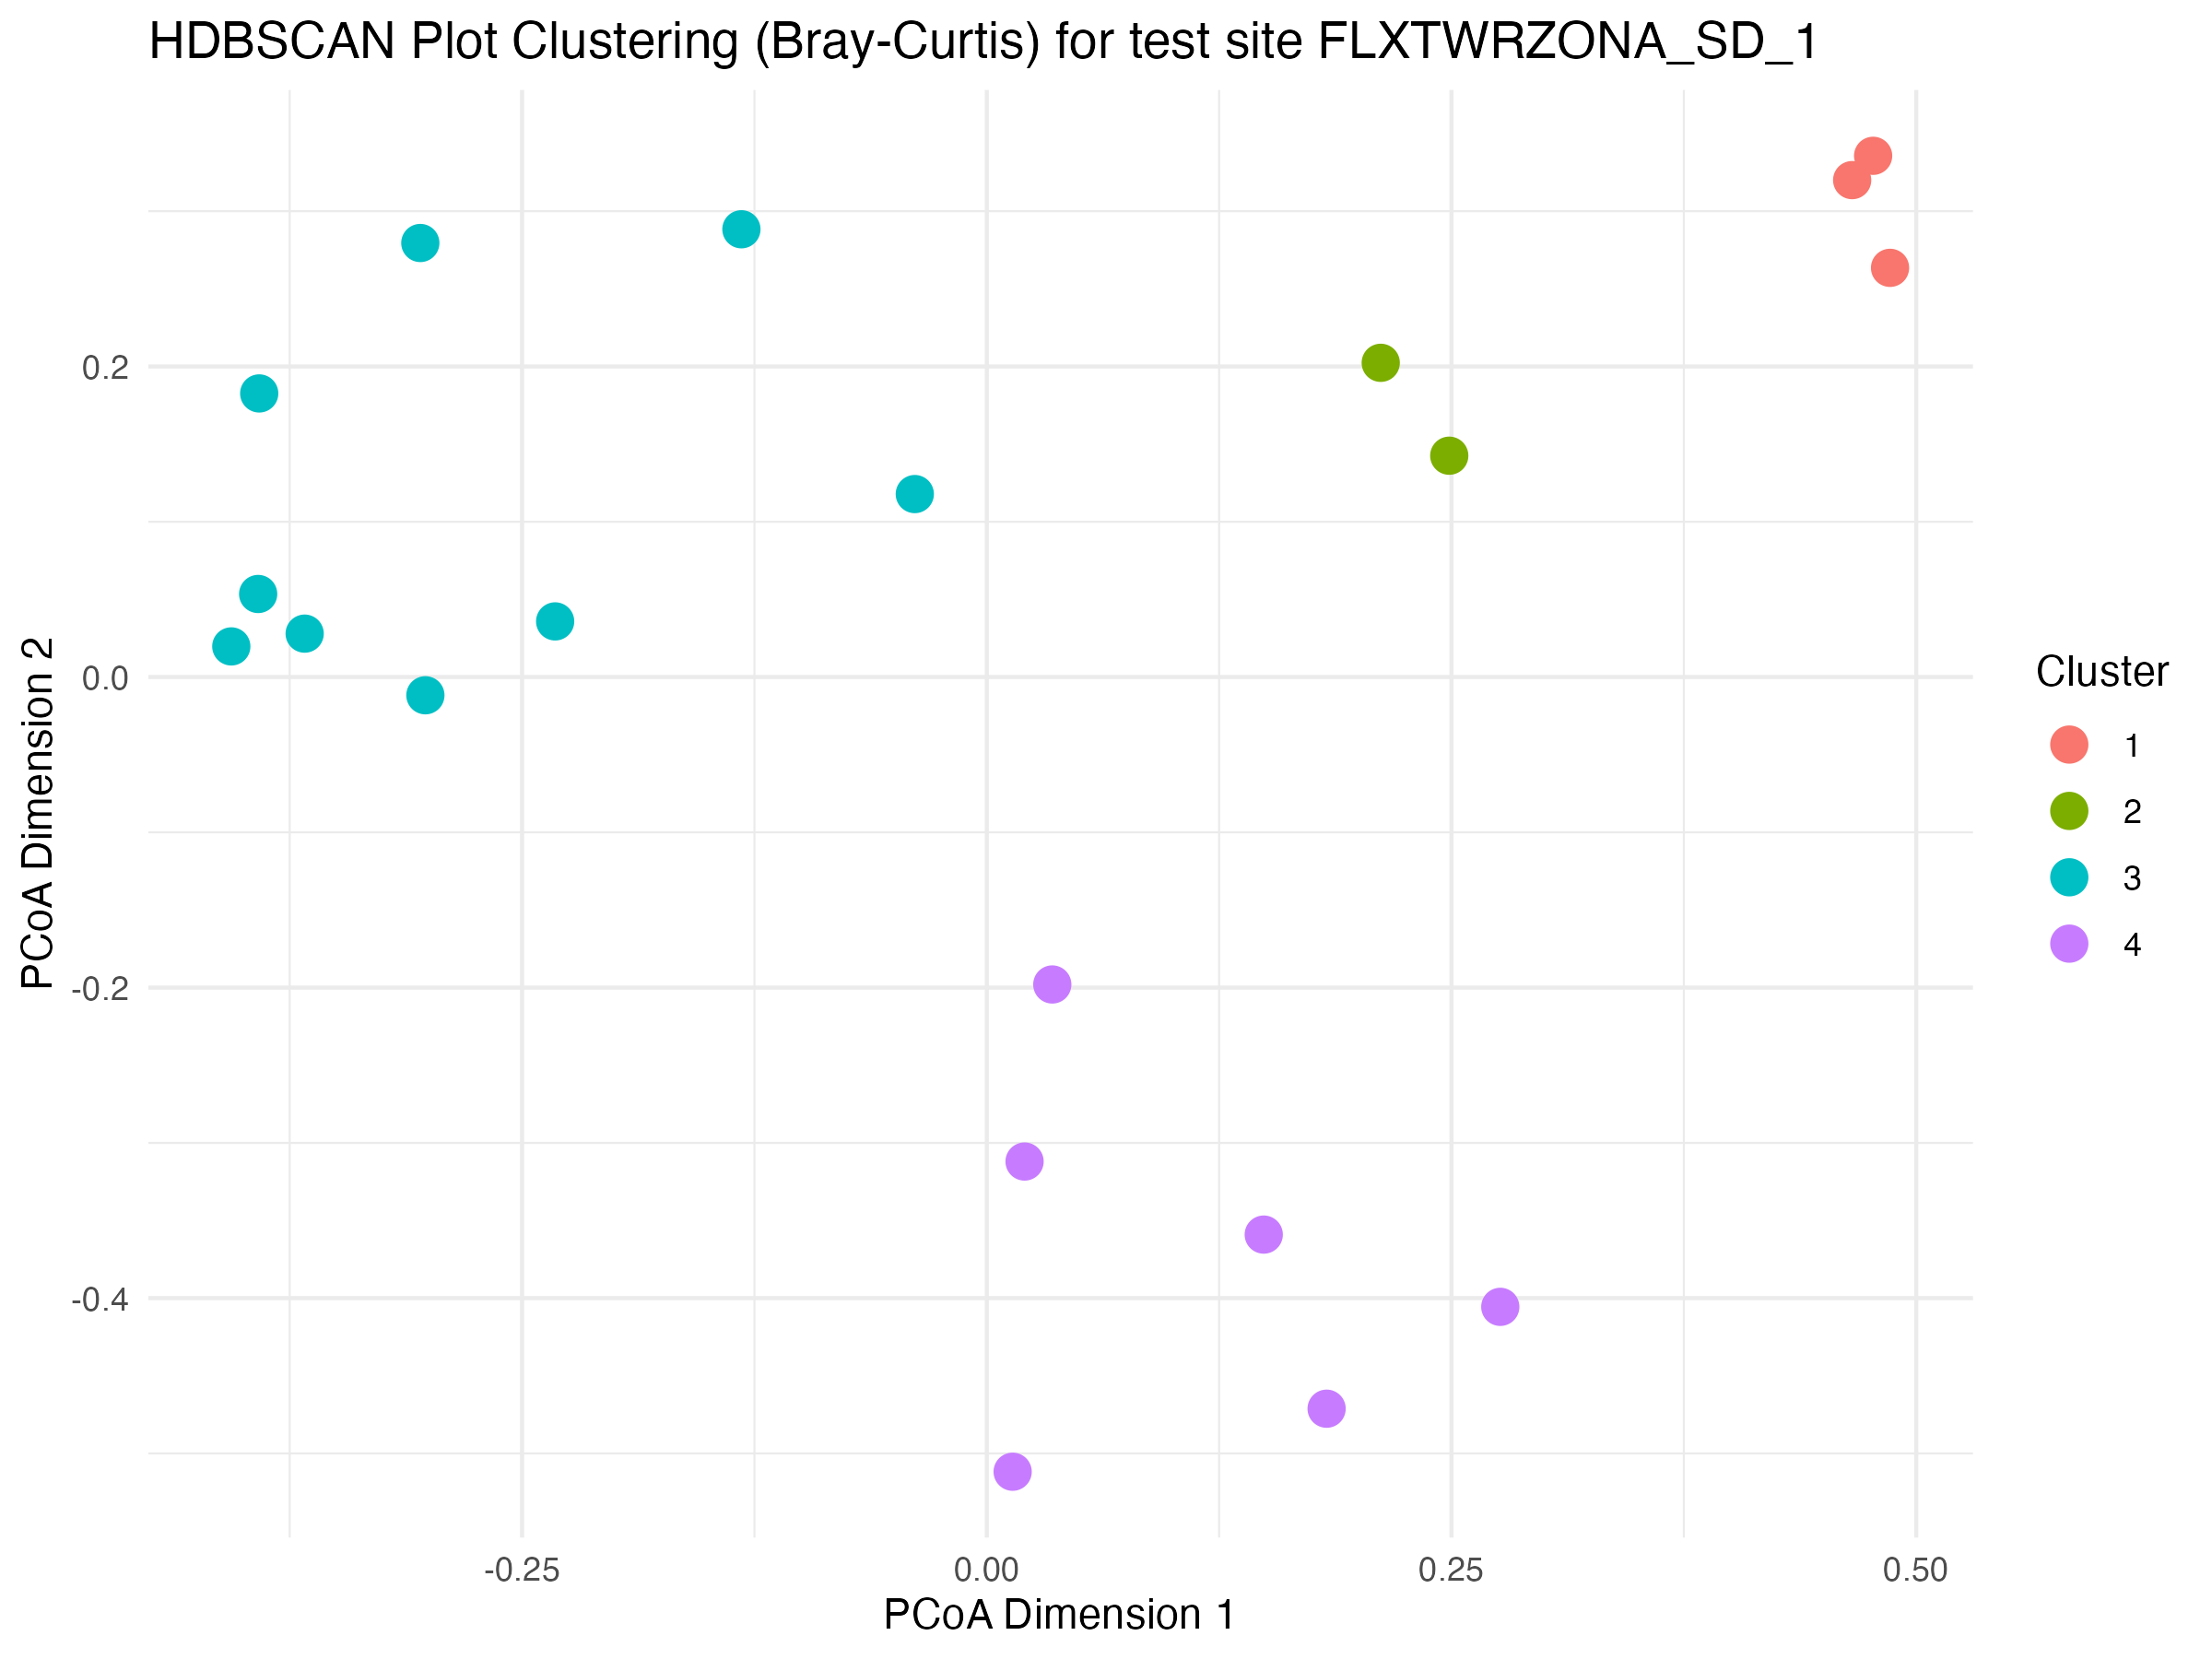
\includegraphics[width=0.9\textwidth]{Figures/Appendix/PlantCommunityClustering/FLXTWRZONA_SD_1_HDBSCAN_clusters.png} % Replace with your actual image path
    \caption{Community cluster HDBSCAN plot for test site FLXTWRZONA\_SD\_1}
    \label{fig:FLXTWRZONA_SD_1_HDBSCAN_clusters}
\end{figure}

\begin{figure}[H]
    \centering
    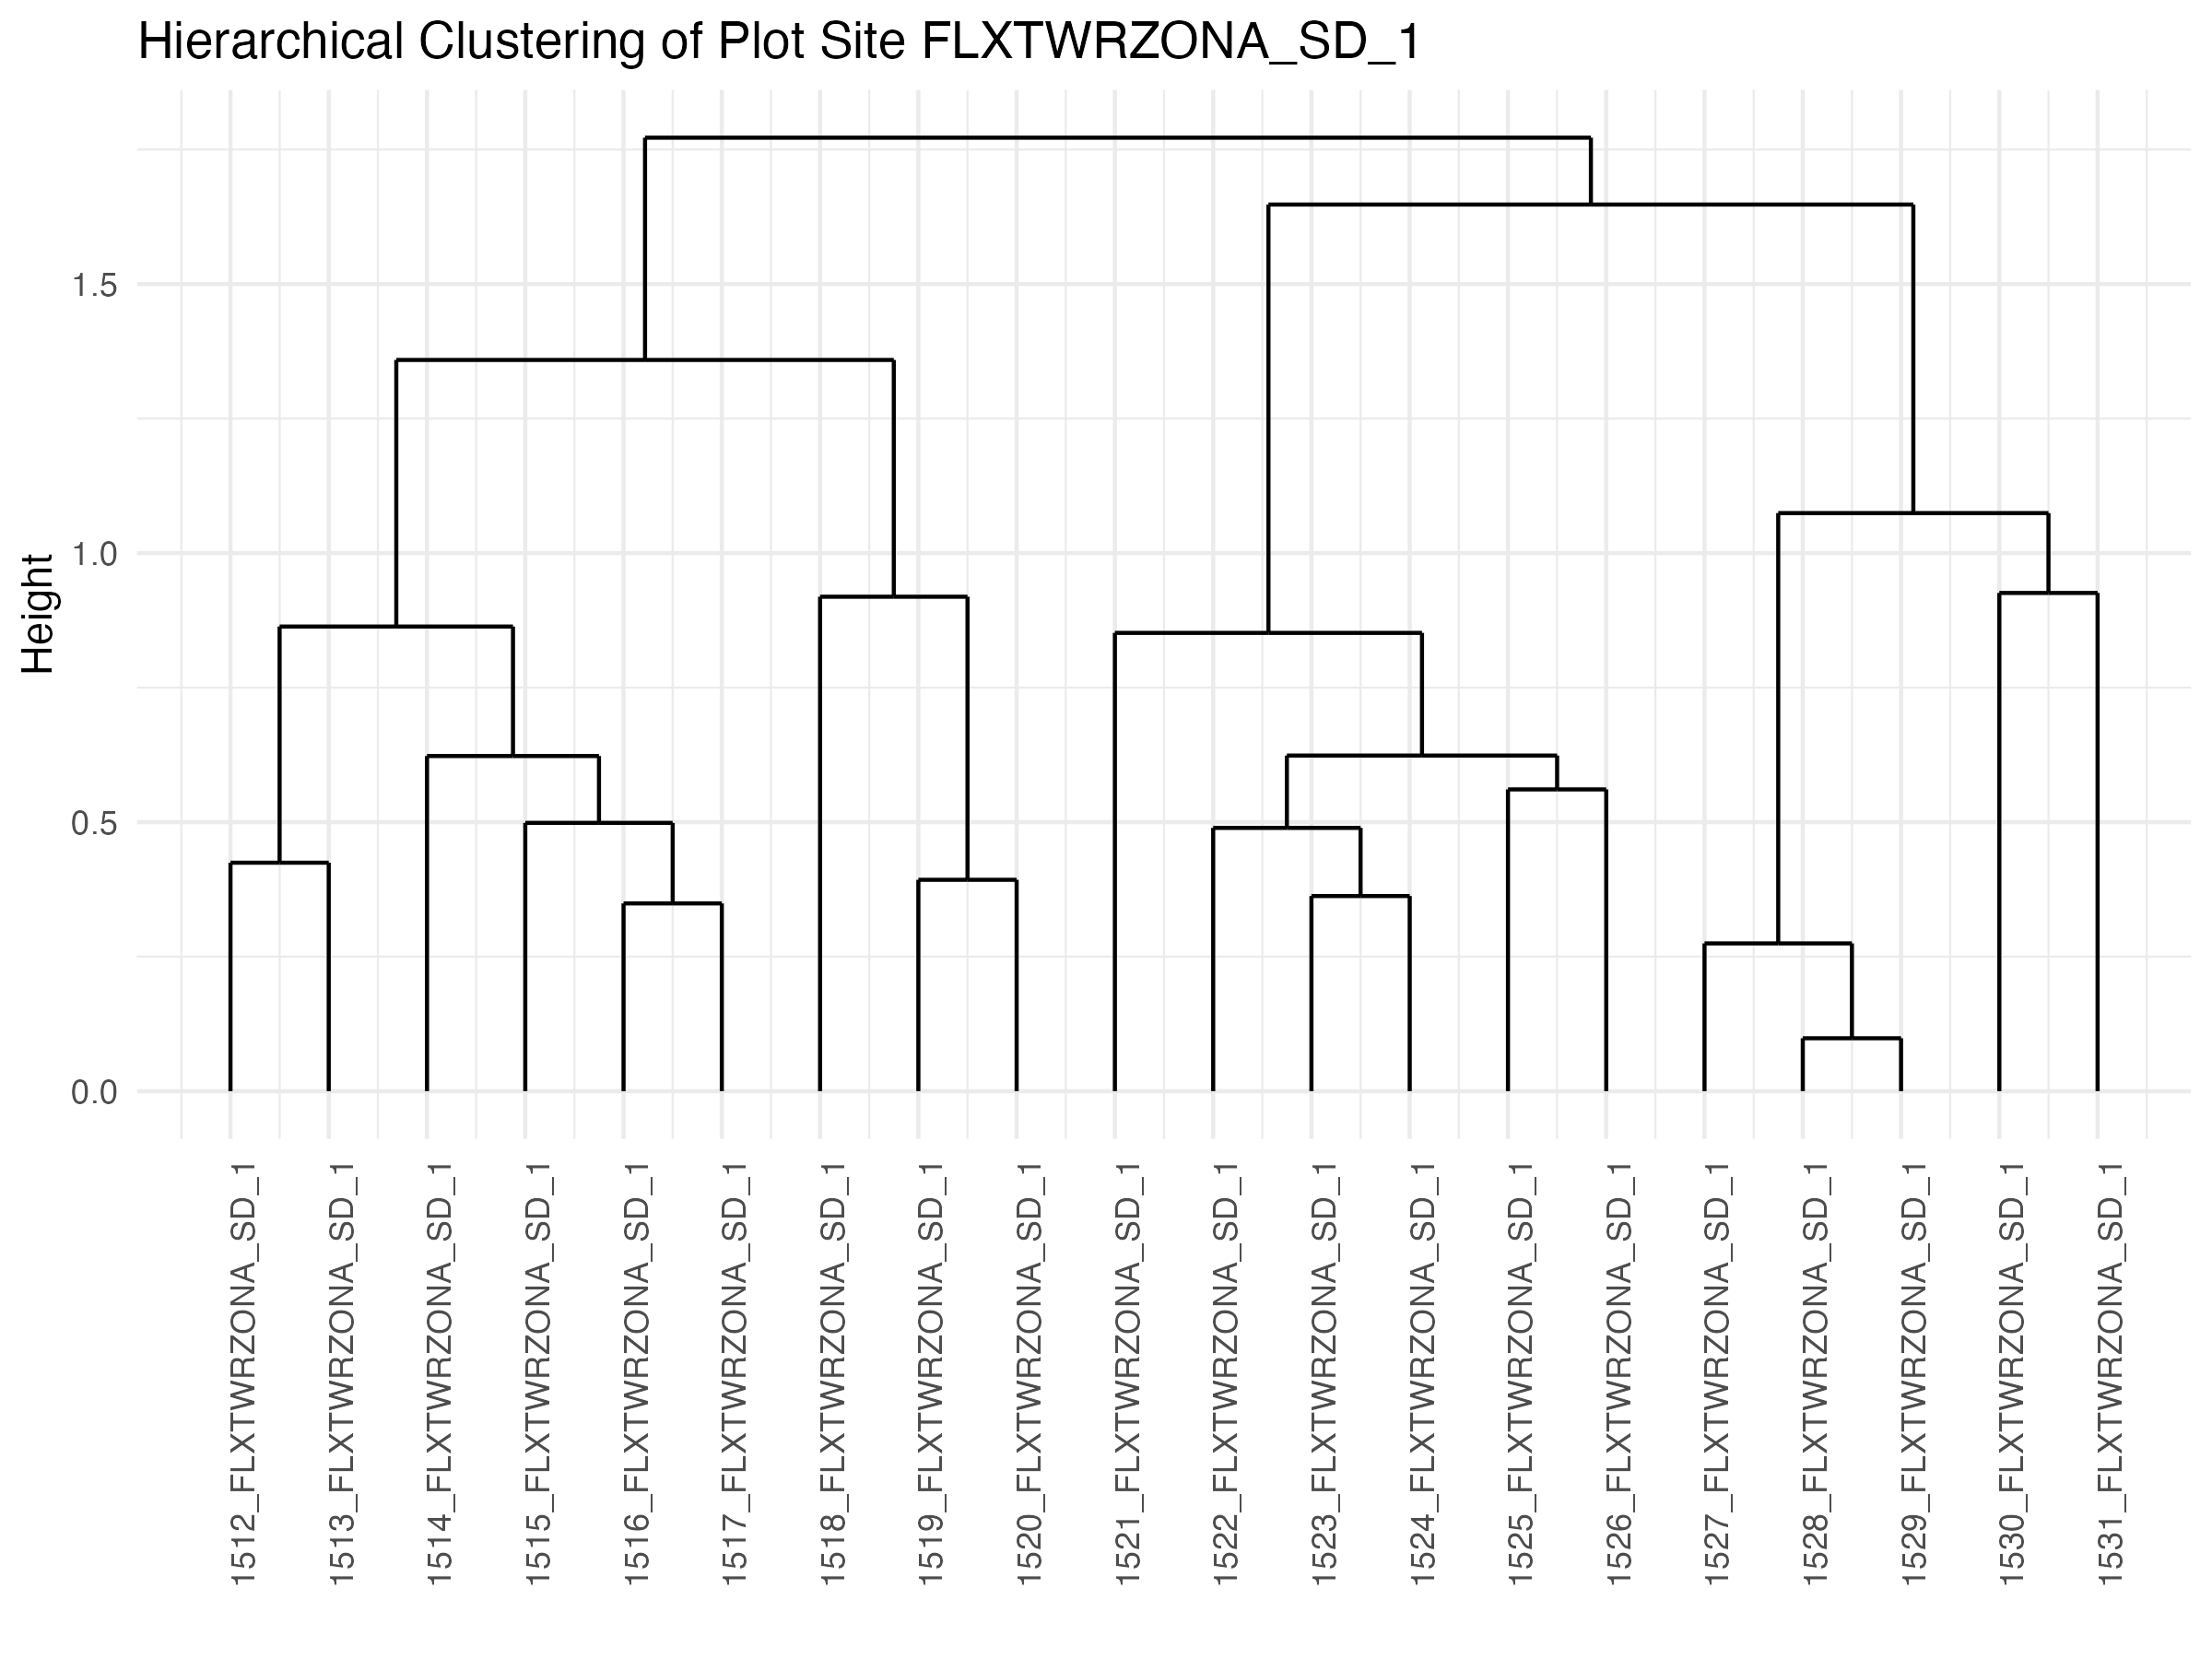
\includegraphics[width=0.9\textwidth]{Figures/Appendix/PlantCommunityClustering/FLXTWRZONA_SD_1_DENDRO.png} % Replace with your actual image path
    \caption{Community cluster dendrogram plot for test site FLXTWRZONA\_SD\_1}
    \label{fig:FLXTWRZONA_SD_1_DENDRO}
\end{figure}

\subsection{FLXTWRZONA\_SD\_2}
\begin{figure}[H]
    \centering
    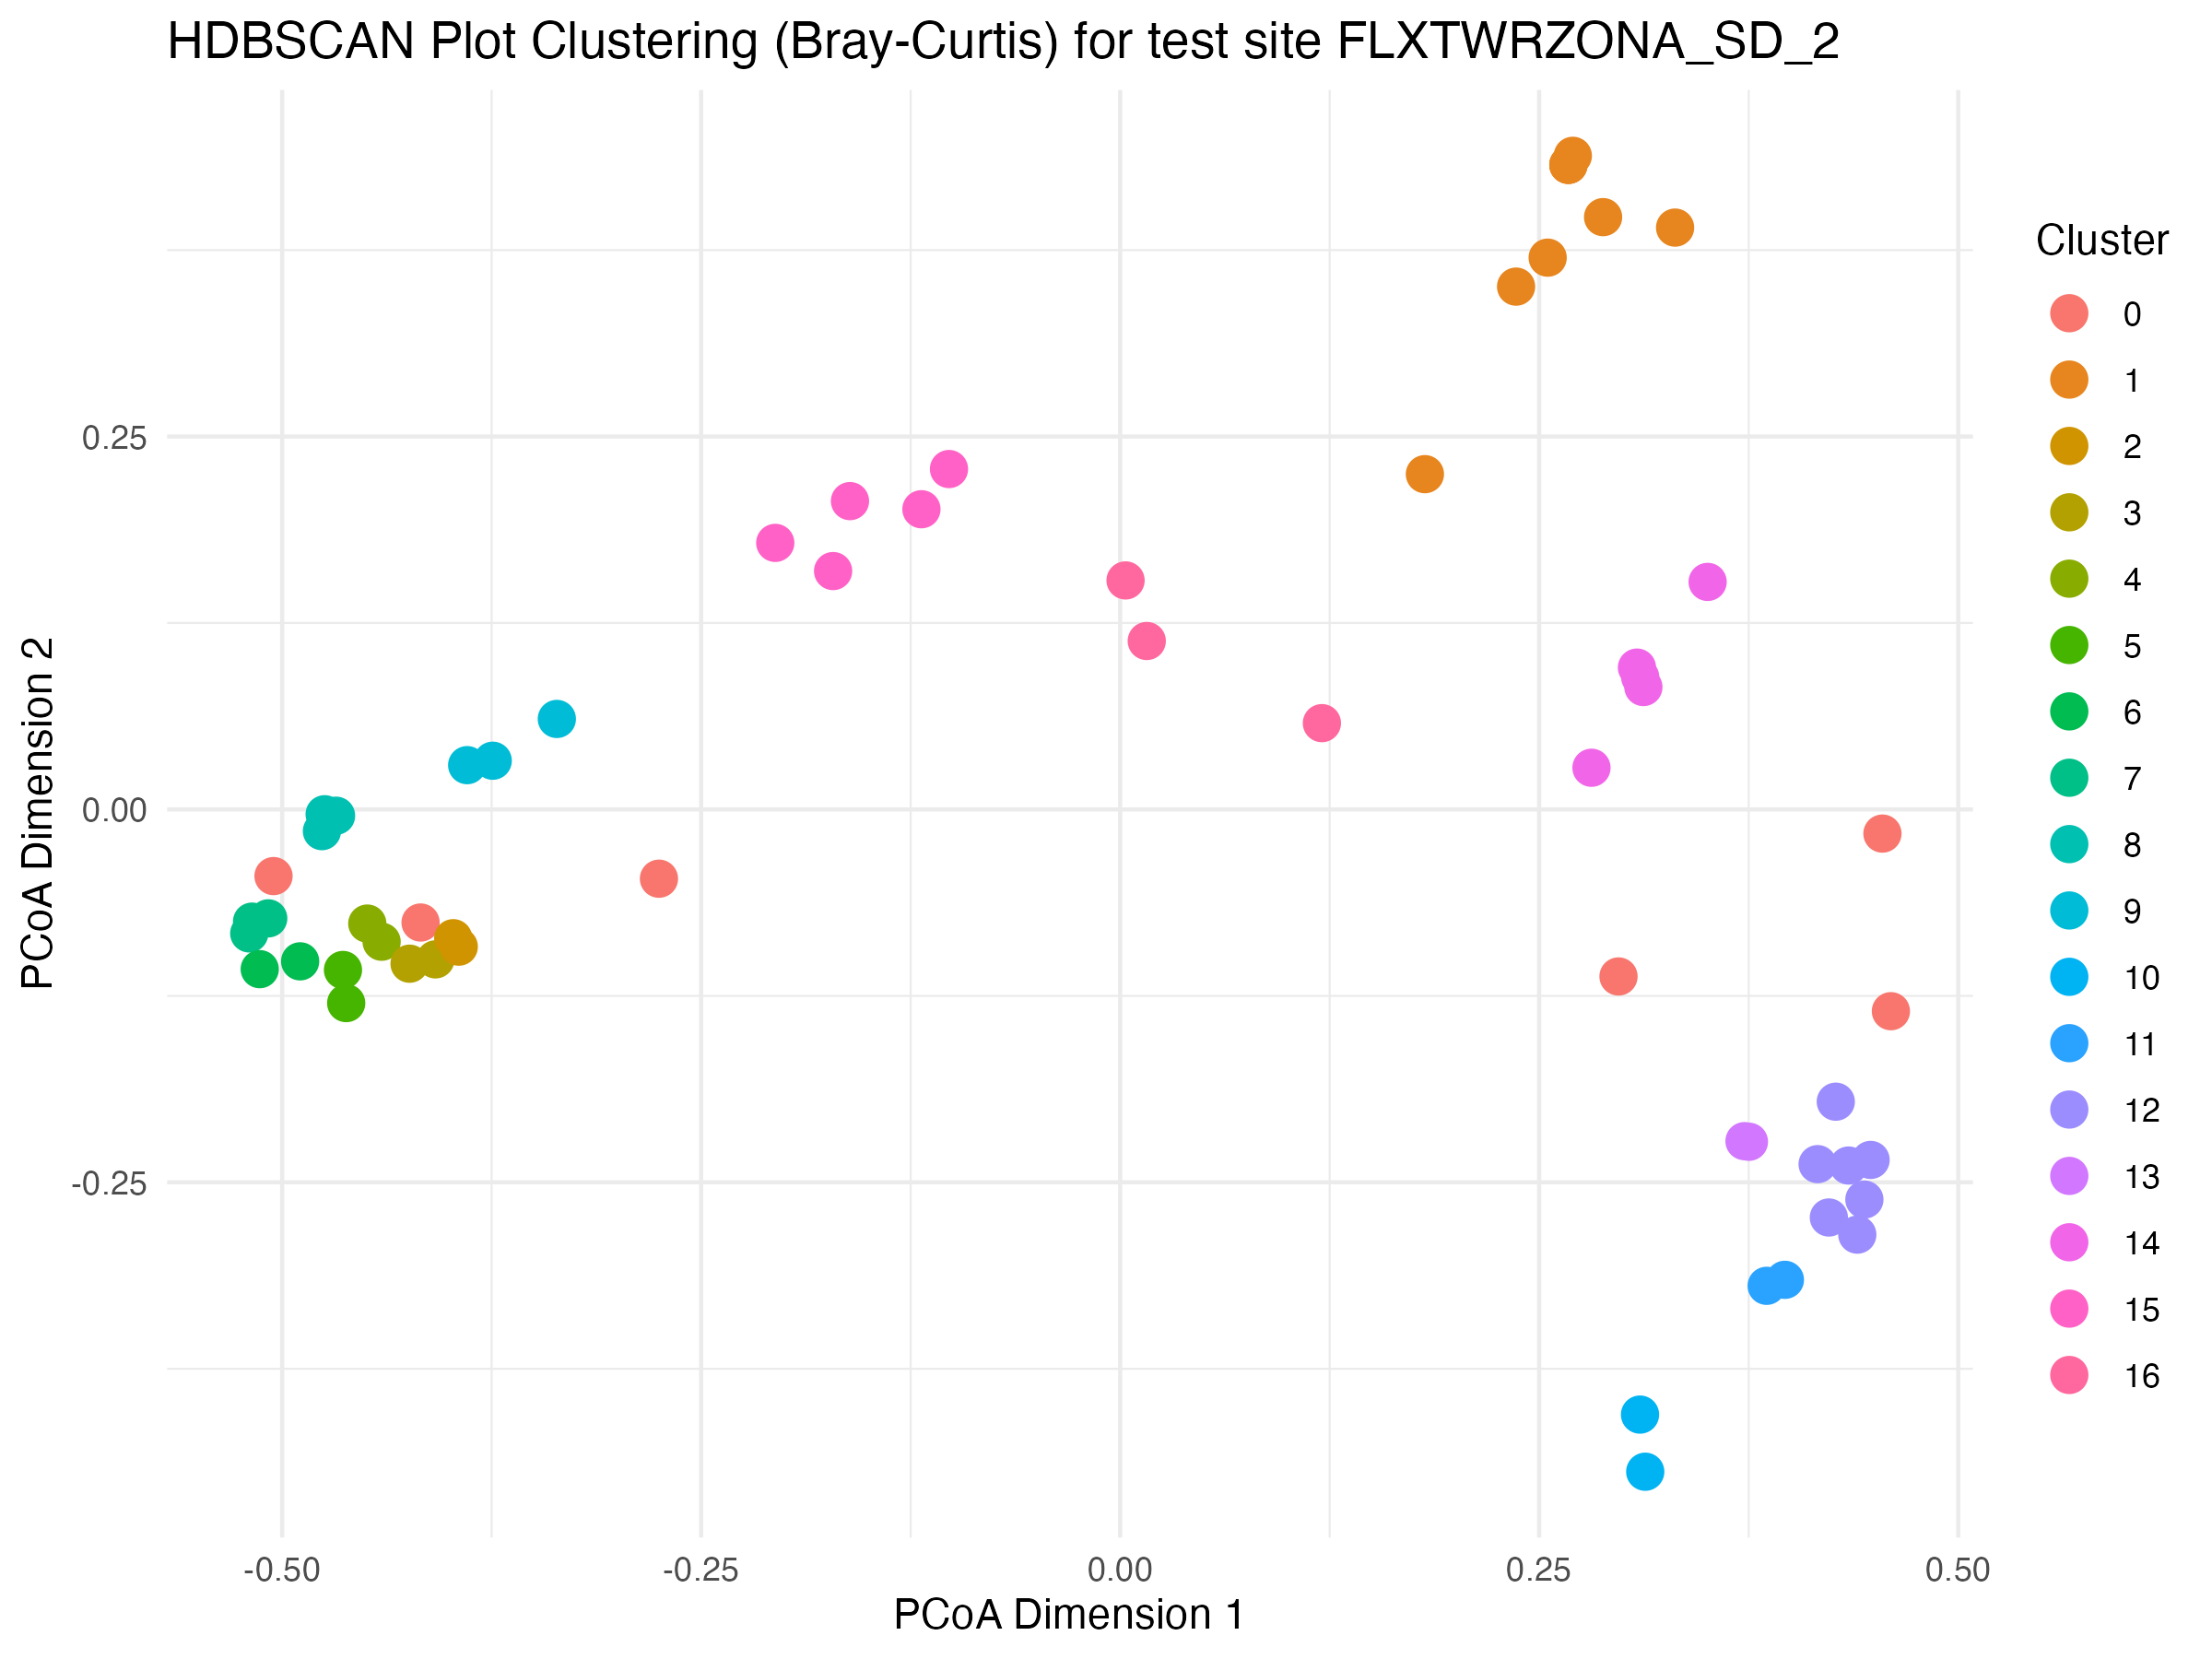
\includegraphics[width=0.9\textwidth]{Figures/Appendix/PlantCommunityClustering/FLXTWRZONA_SD_2_HDBSCAN_clusters.png} % Replace with your actual image path
    \caption{Community cluster HDBSCAN plot for test site FLXTWRZONA\_SD\_2}
    \label{fig:FLXTWRZONA_SD_2_HDBSCAN_clusters}
\end{figure}

\begin{figure}[H]
    \centering
    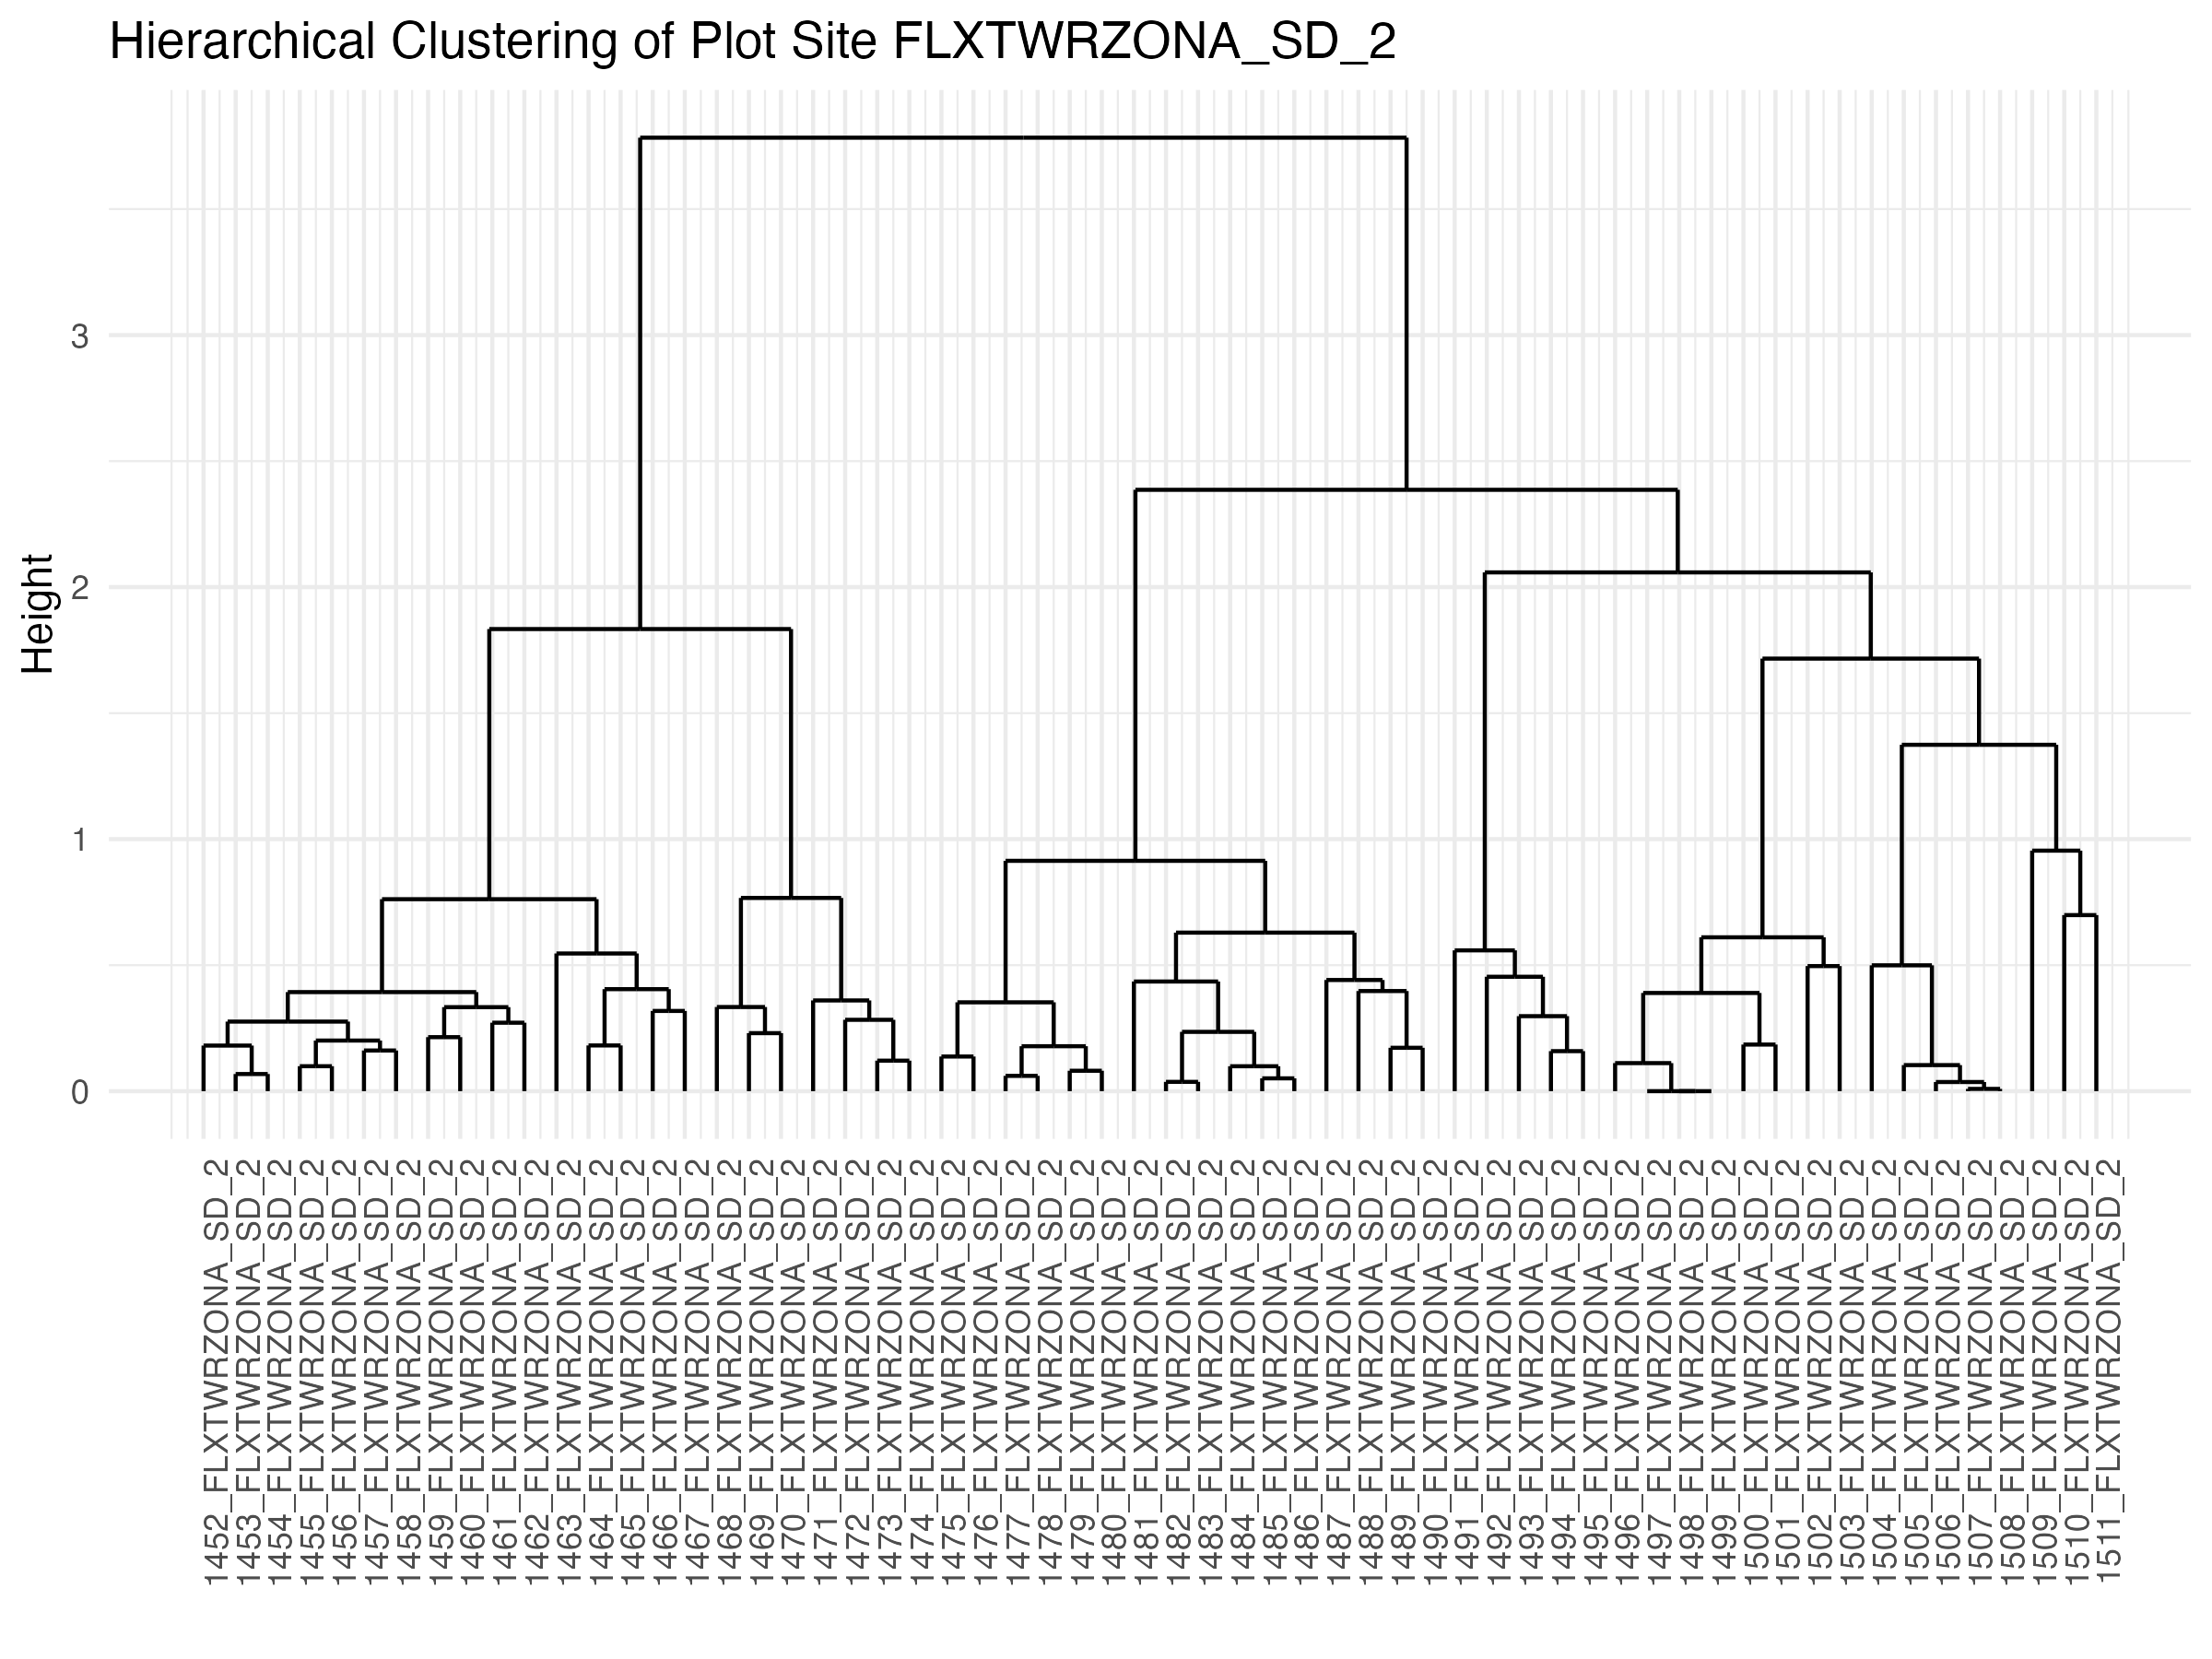
\includegraphics[width=0.9\textwidth]{Figures/Appendix/PlantCommunityClustering/FLXTWRZONA_SD_2_DENDRO.png} % Replace with your actual image path
    \caption{Community cluster dendrogram plot for test site FLXTWRZONA\_SD\_2}
    \label{fig:FLXTWRZONA_SD_2_DENDRO}
\end{figure}

\subsection{FLXTWRZONA\_SD\_3}
\begin{figure}[H]
    \centering
    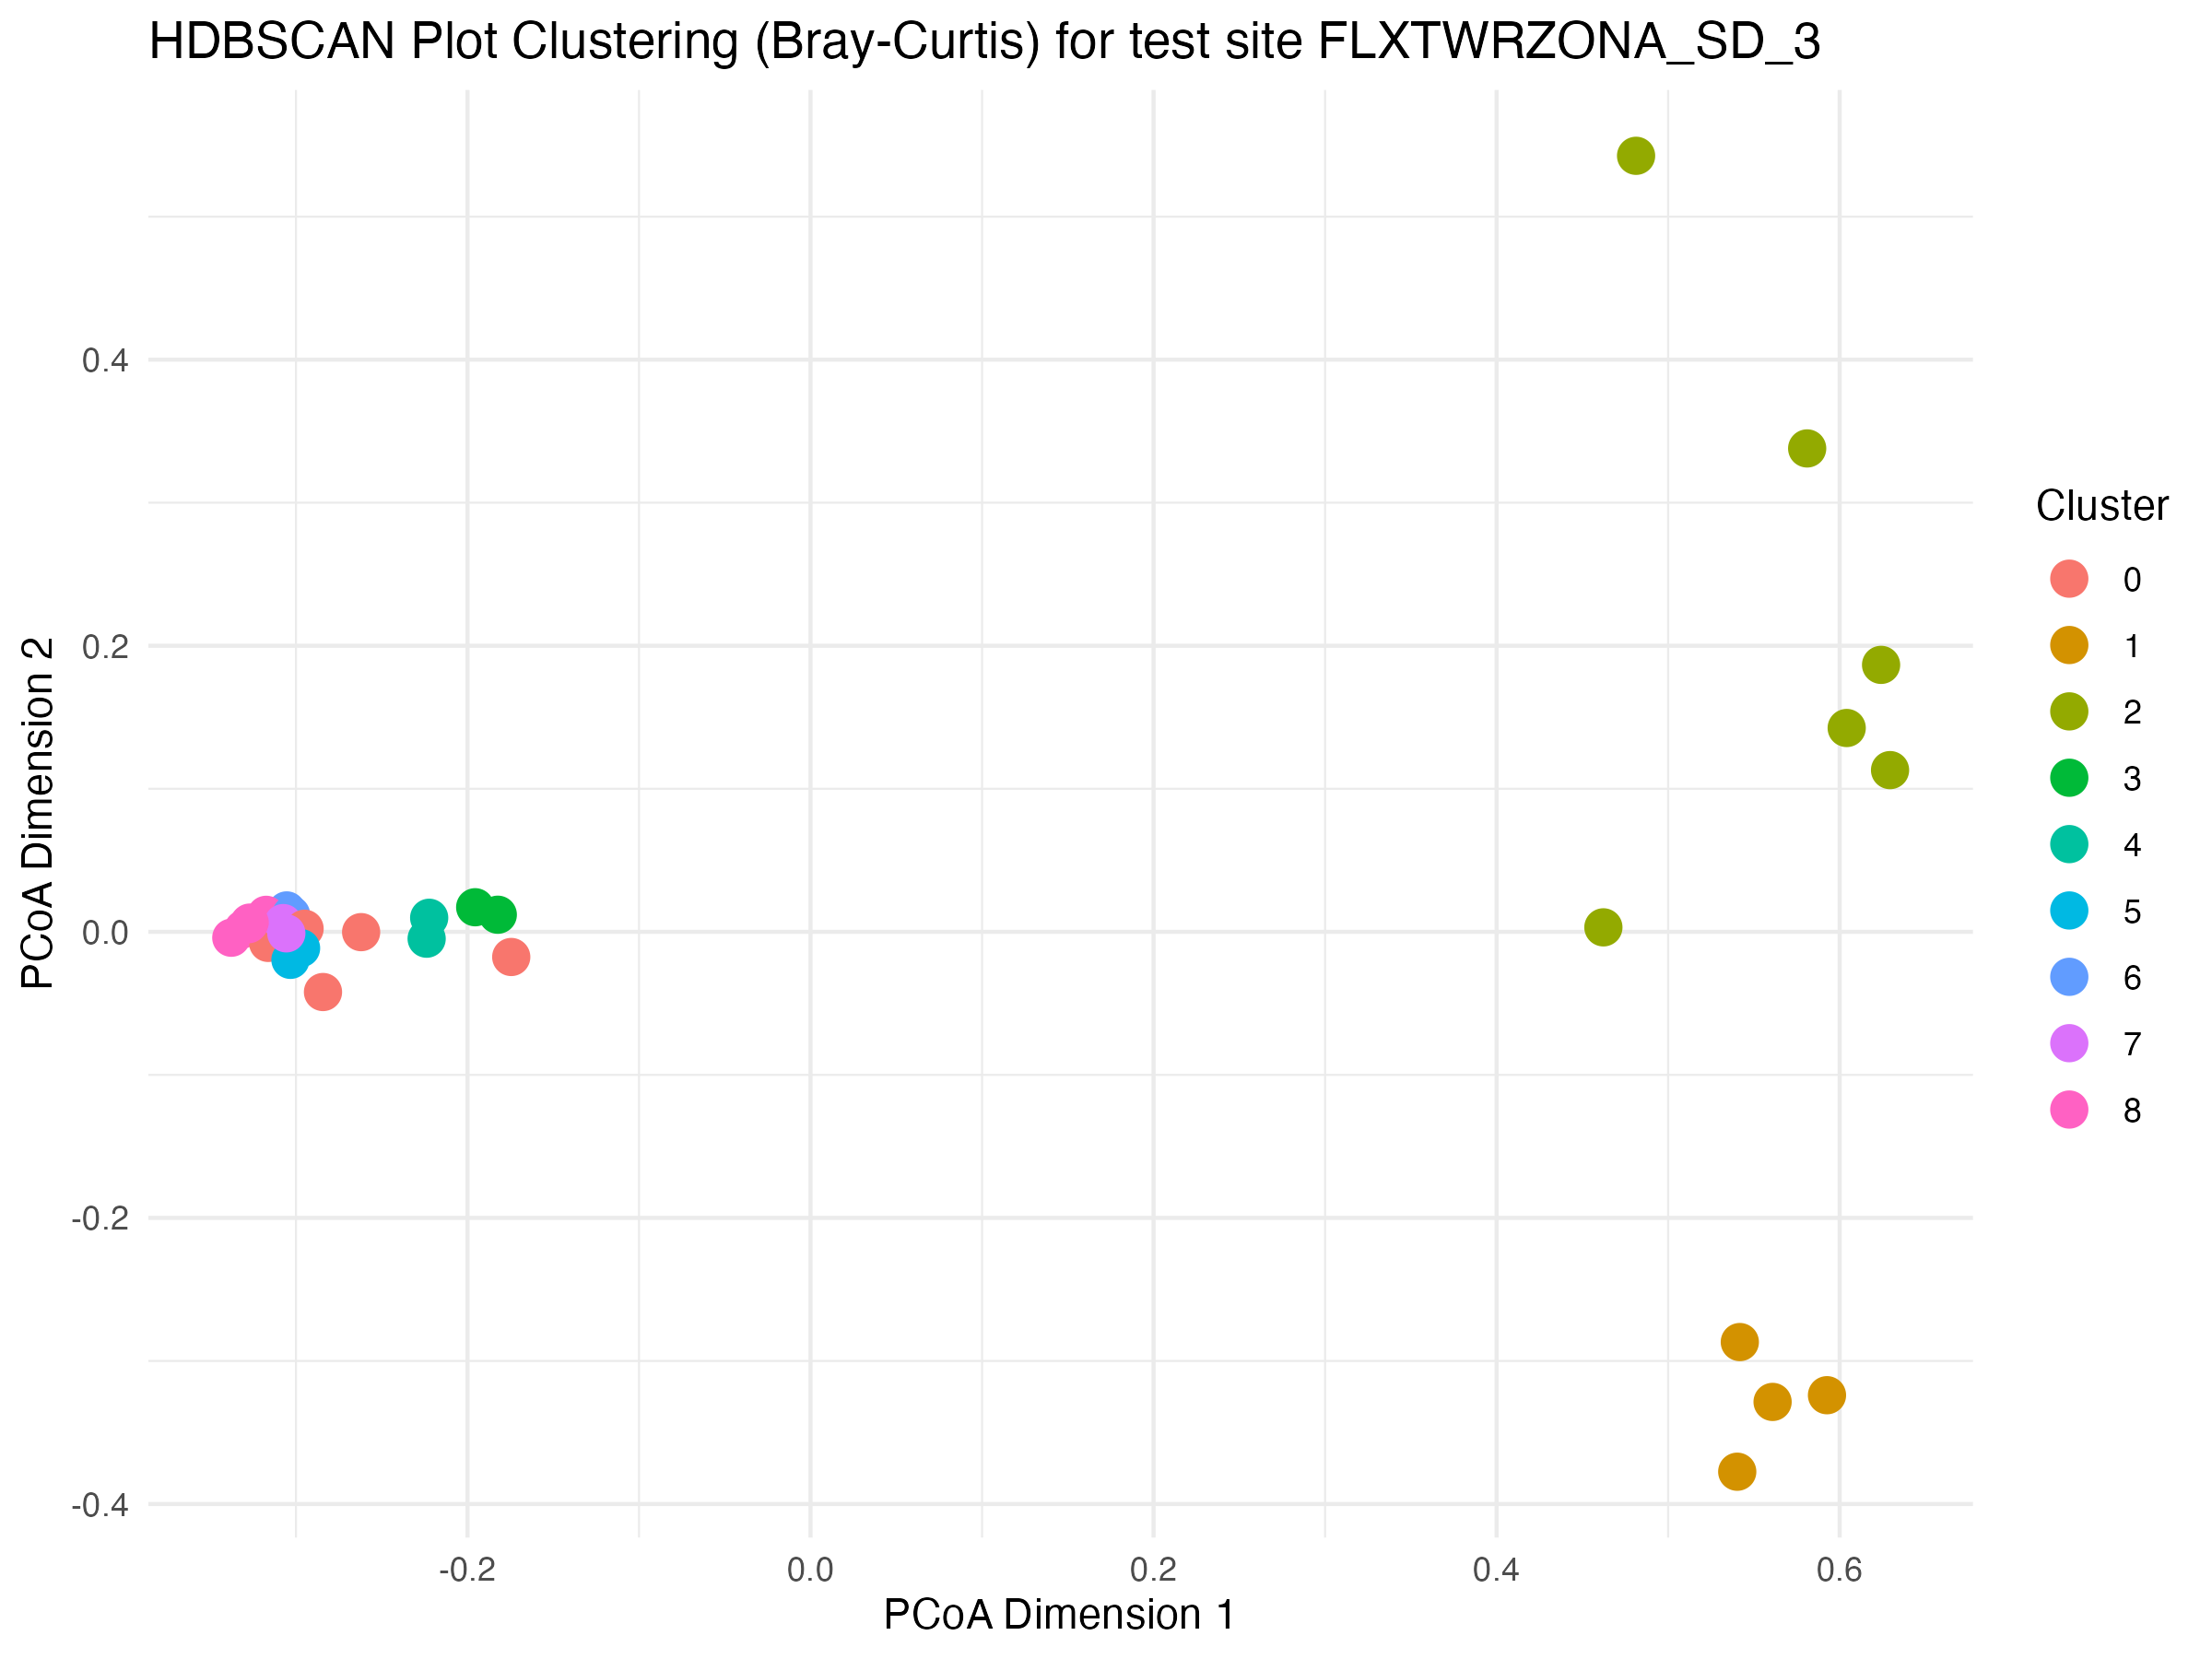
\includegraphics[width=0.9\textwidth]{Figures/Appendix/PlantCommunityClustering/FLXTWRZONA_SD_3_HDBSCAN_clusters.png} % Replace with your actual image path
    \caption{Community cluster HDBSCAN plot for test site FLXTWRZONA\_SD\_3}
    \label{fig:FLXTWRZONA_SD_3_HDBSCAN_clusters}
\end{figure}

\begin{figure}[H]
    \centering
    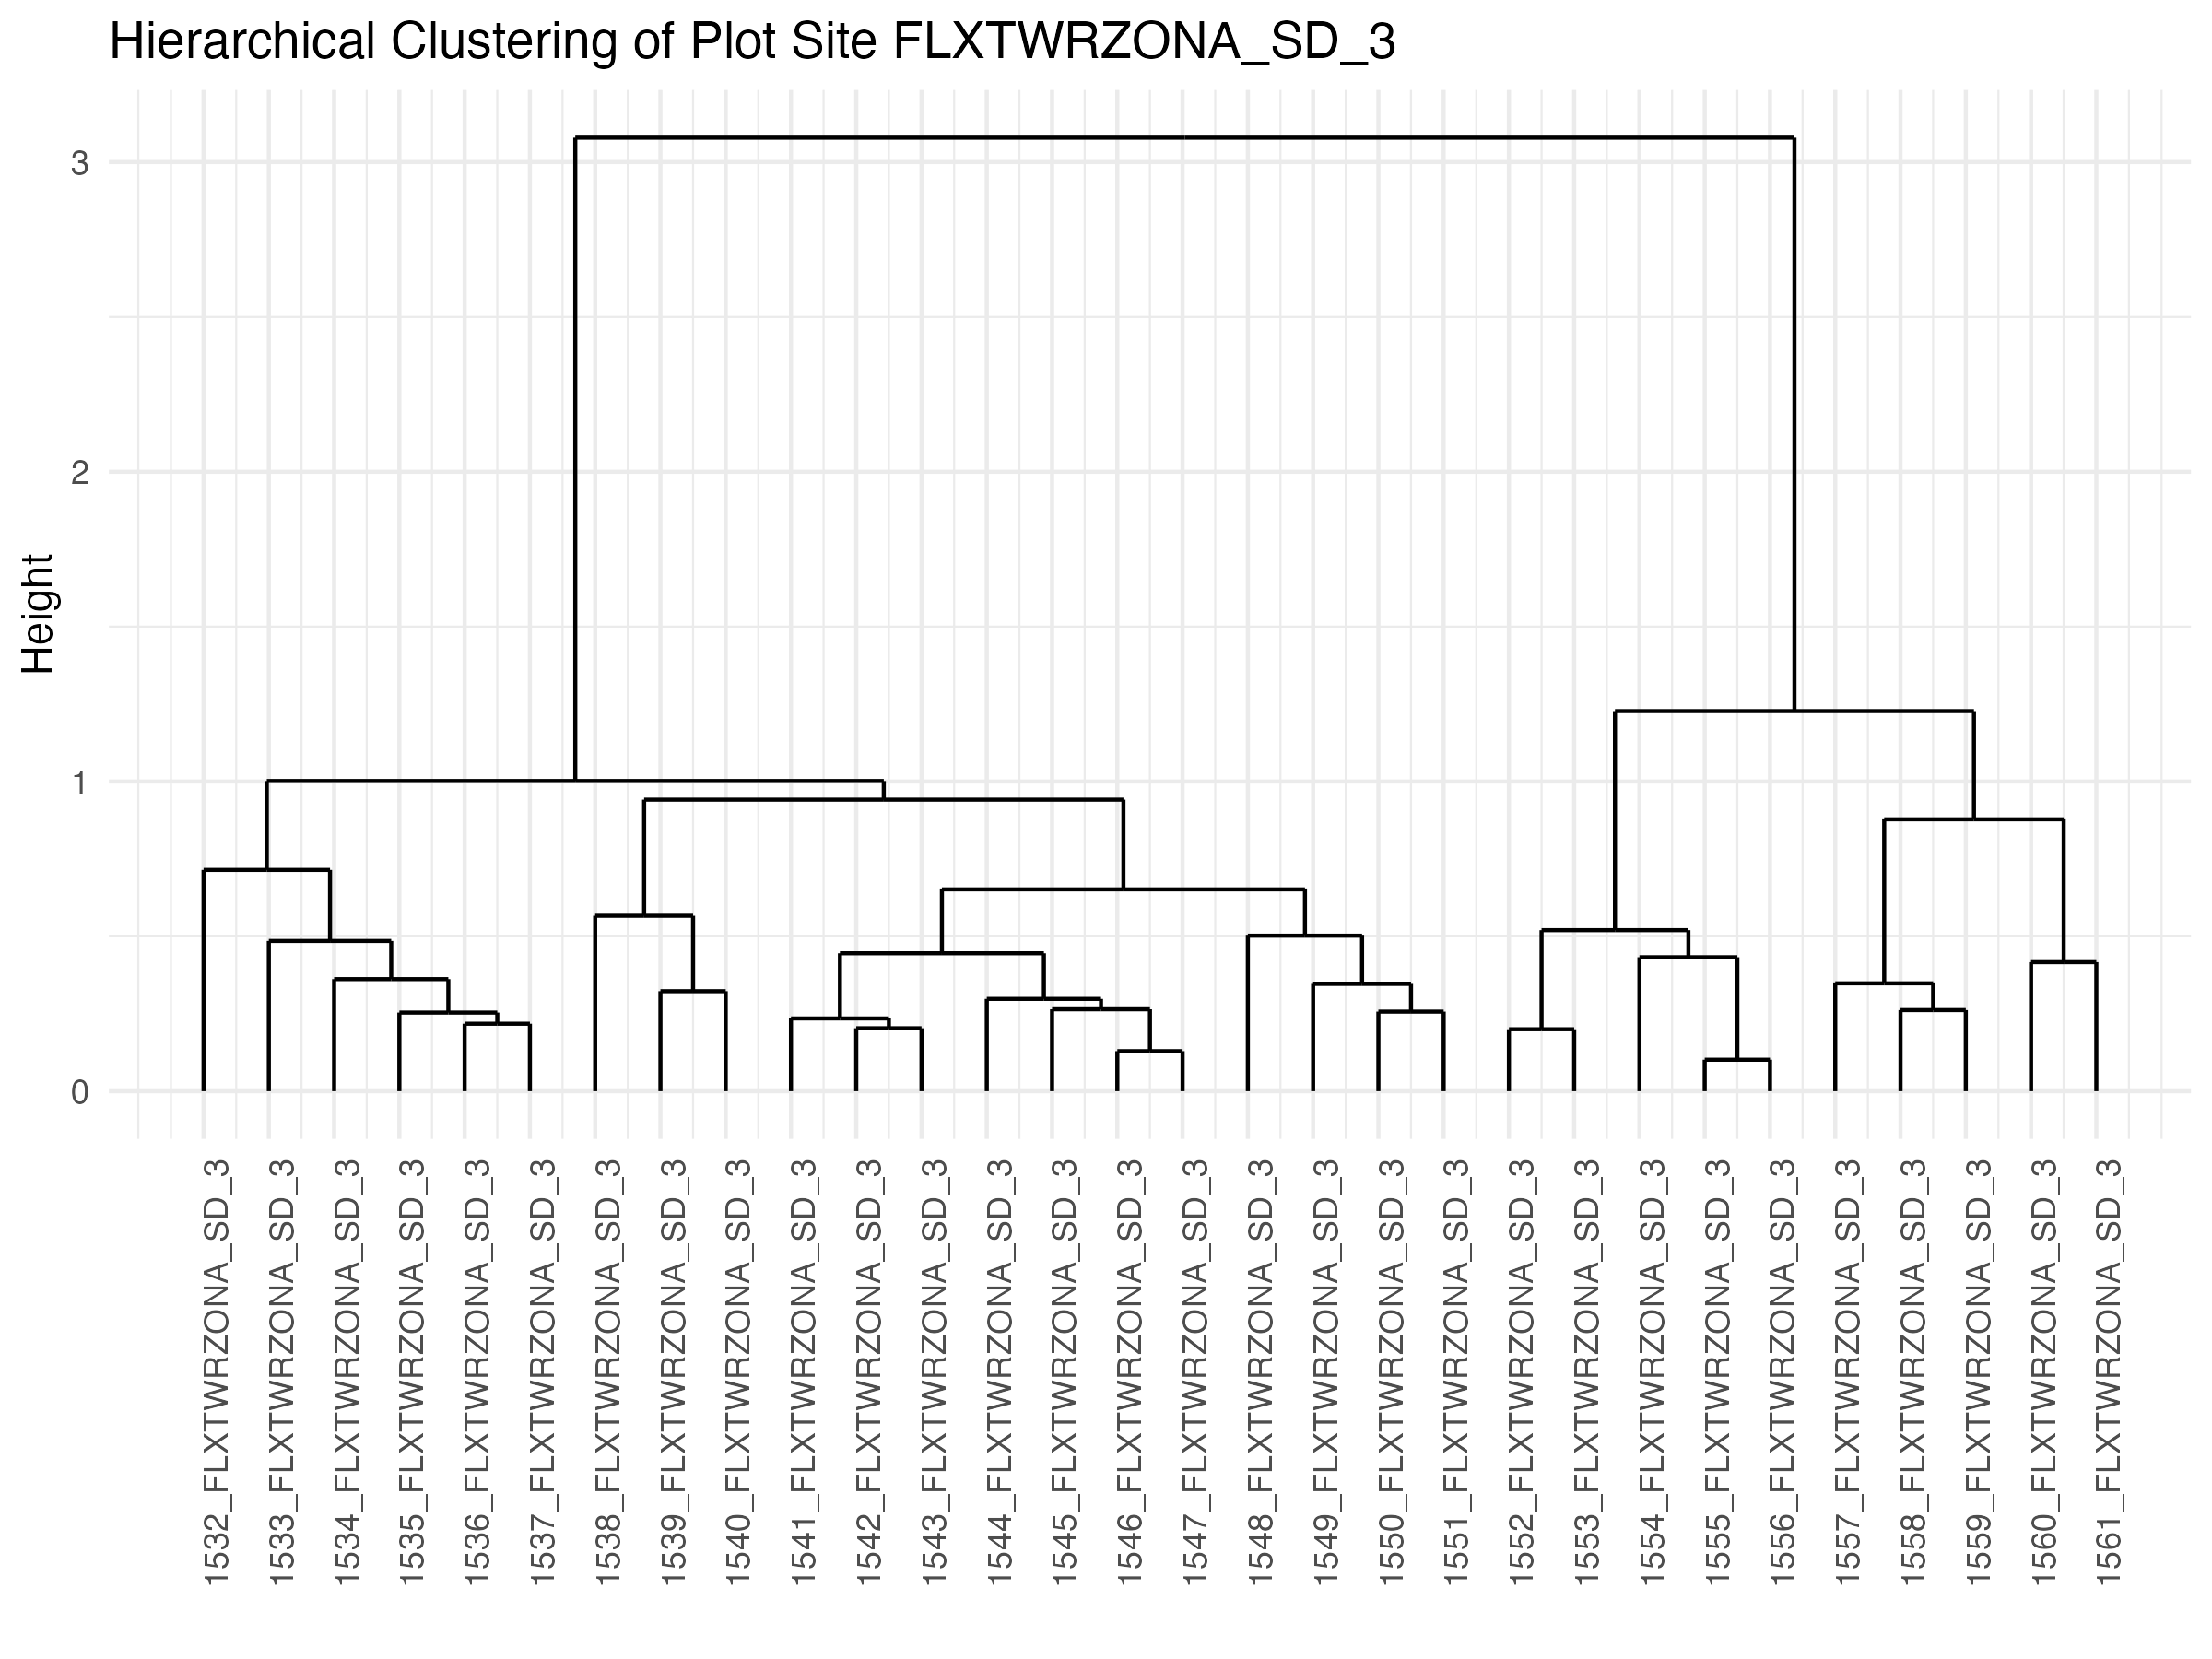
\includegraphics[width=0.9\textwidth]{Figures/Appendix/PlantCommunityClustering/FLXTWRZONA_SD_3_DENDRO.png} % Replace with your actual image path
    \caption{Community cluster dendrogram plot for test site FLXTWRZONA\_SD\_3}
    \label{fig:FLXTWRZONA_SD_3_DENDRO}
\end{figure}

\subsection{FLXTWRZONA\_SD\_4}
\begin{figure}[H]
    \centering
    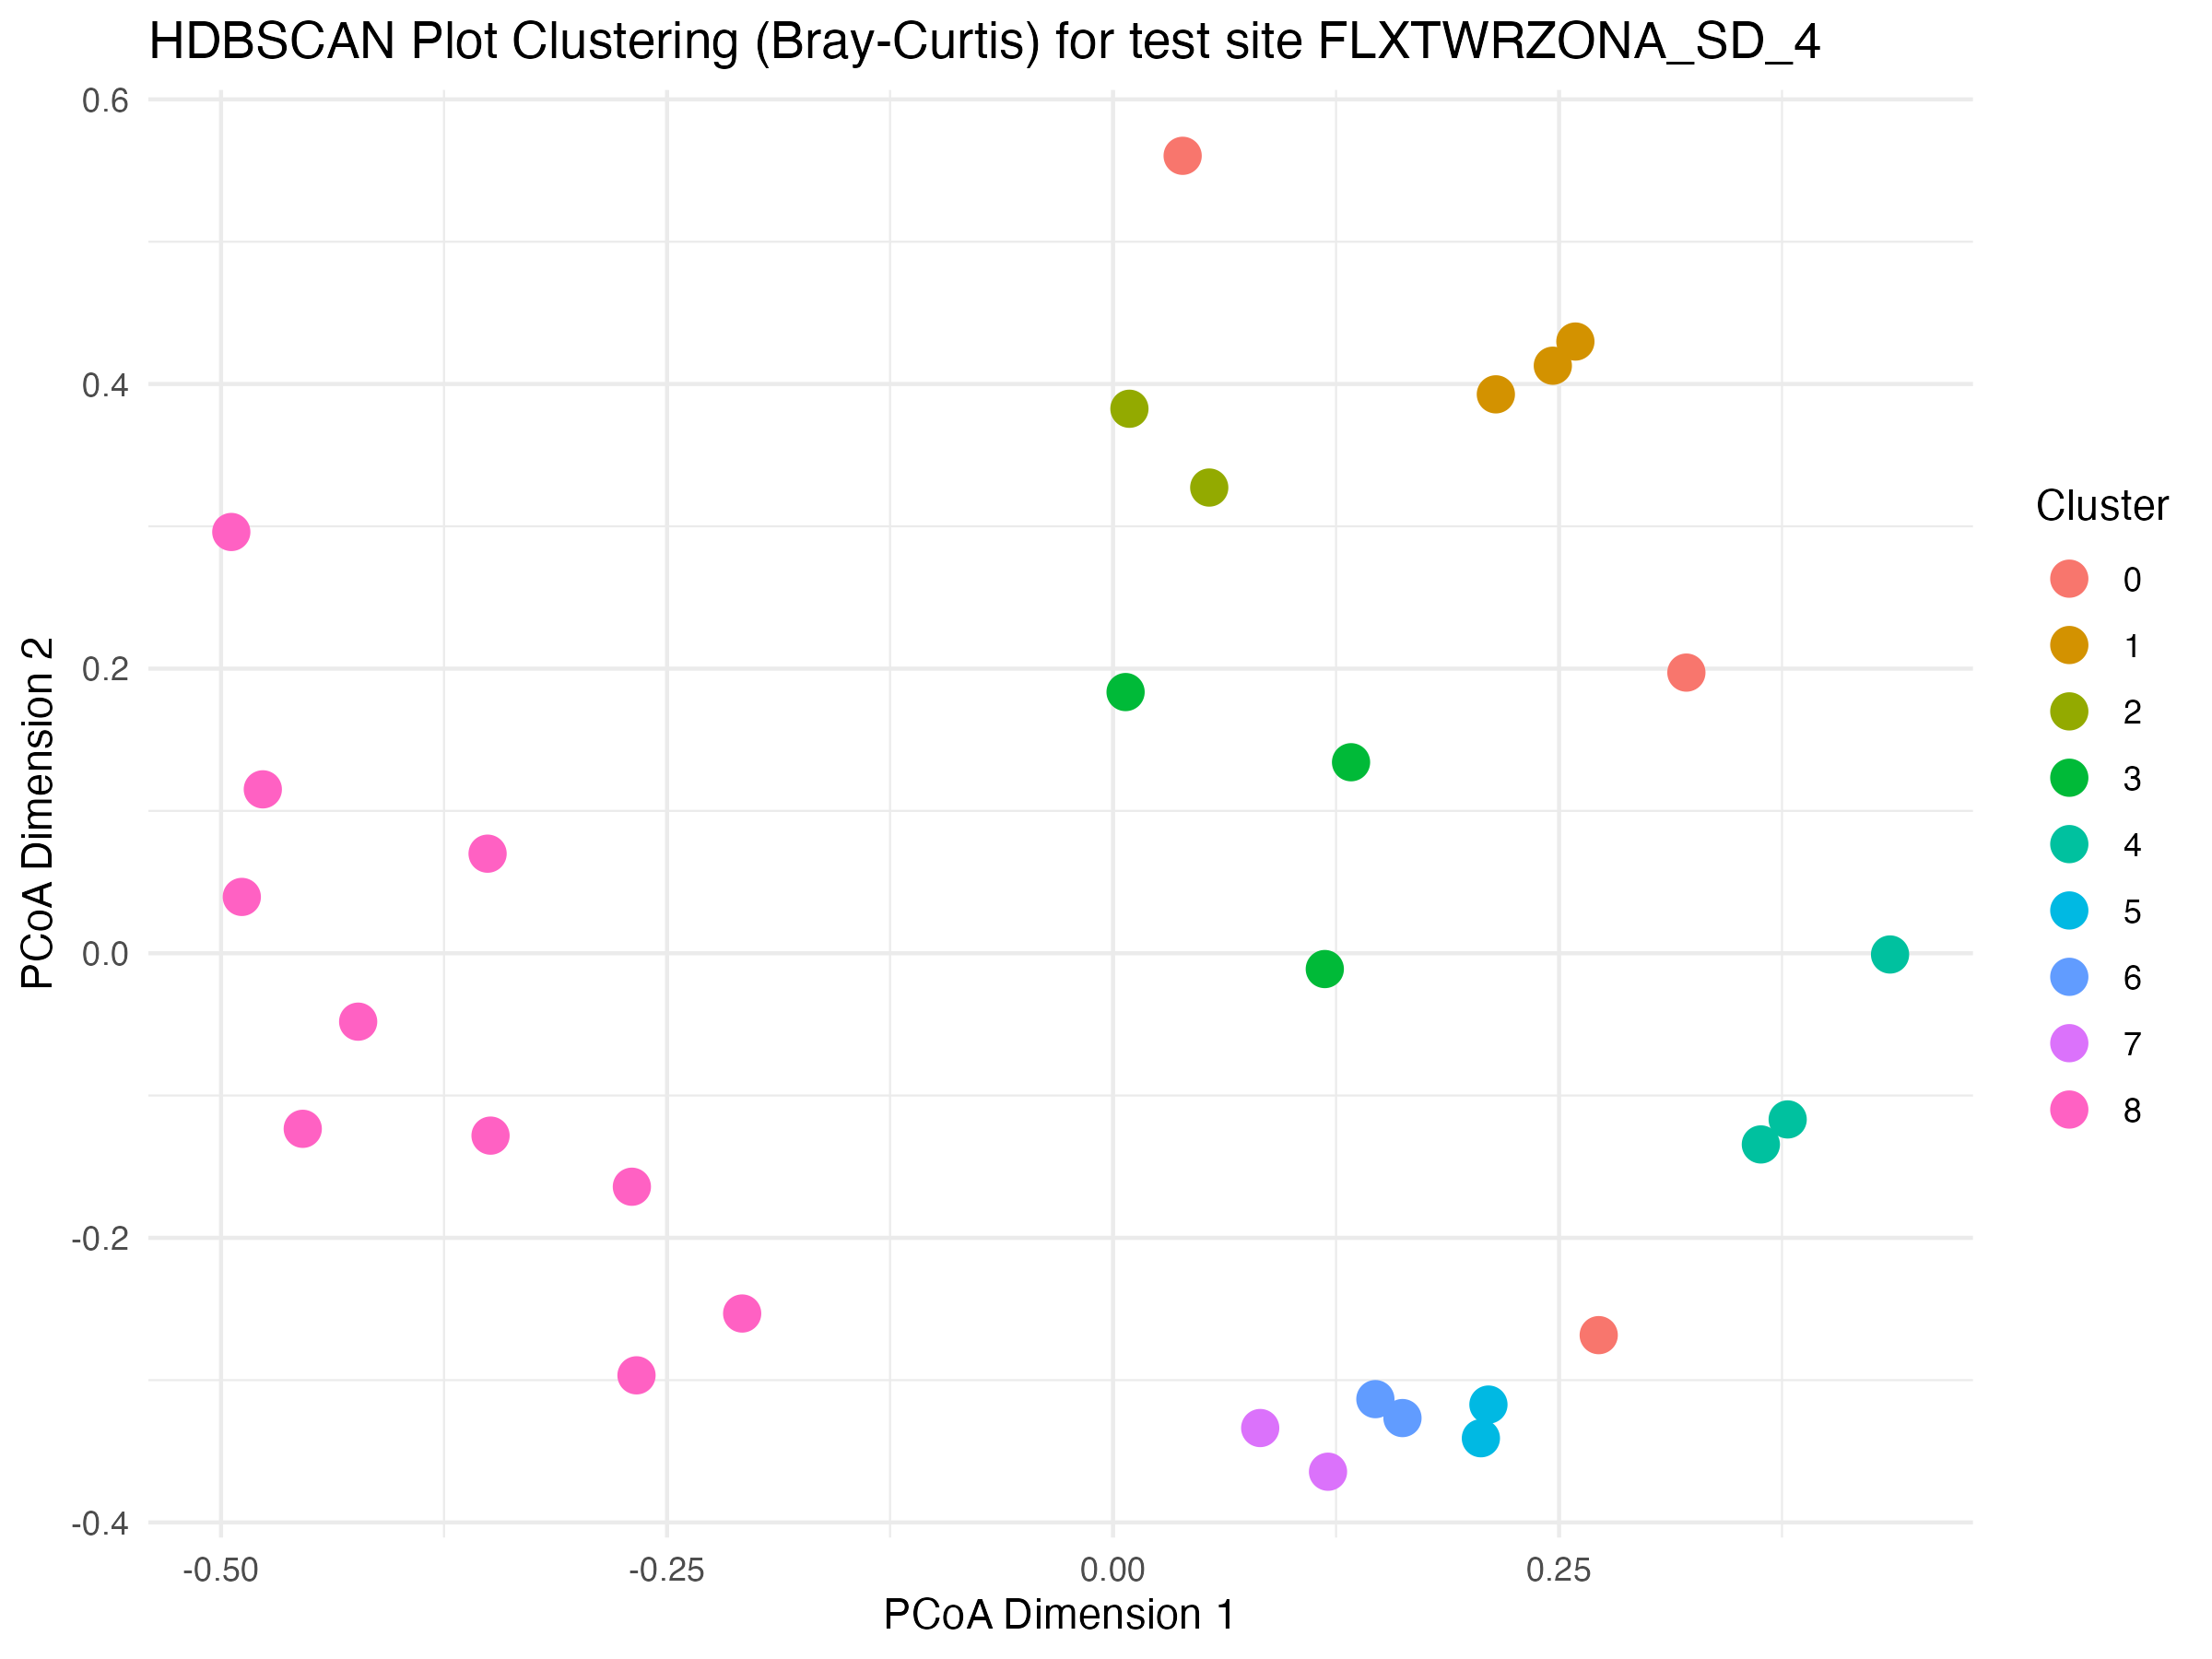
\includegraphics[width=0.9\textwidth]{Figures/Appendix/PlantCommunityClustering/FLXTWRZONA_SD_4_HDBSCAN_clusters.png} % Replace with your actual image path
    \caption{Community cluster HDBSCAN plot for test site FLXTWRZONA\_SD\_4}
    \label{fig:FLXTWRZONA_SD_4_HDBSCAN_clusters}
\end{figure}

\begin{figure}[H]
    \centering
    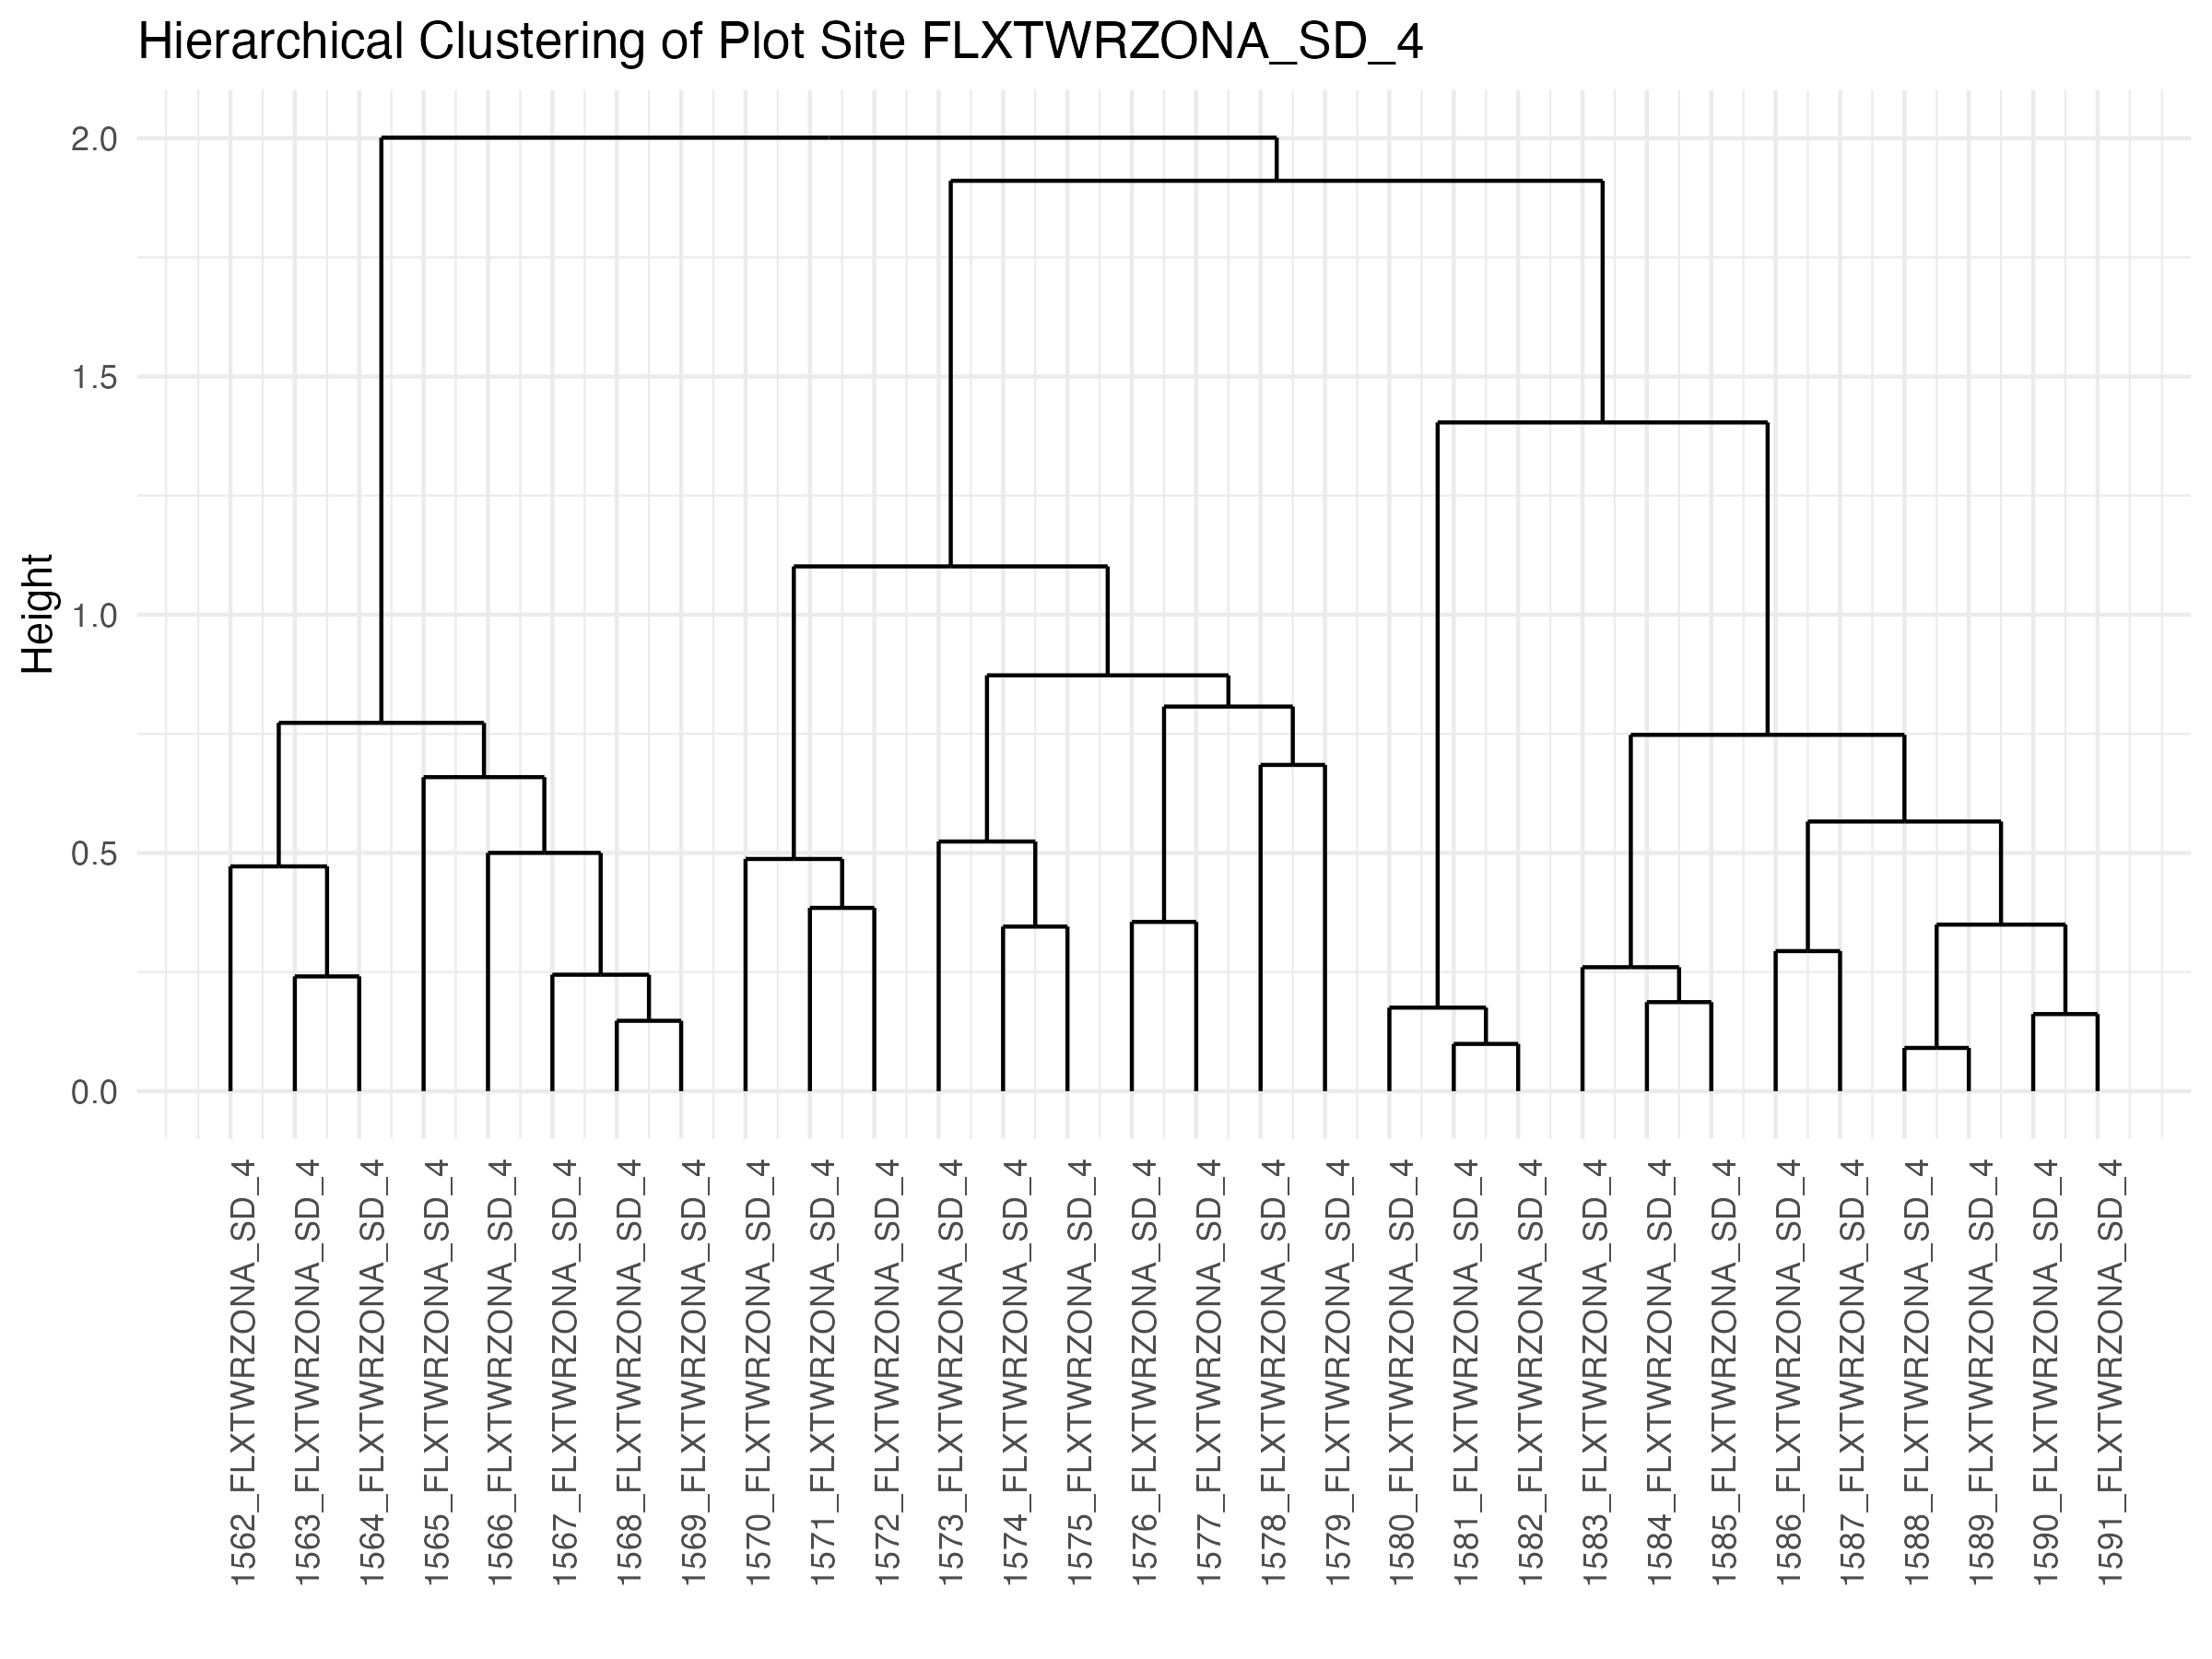
\includegraphics[width=0.9\textwidth]{Figures/Appendix/PlantCommunityClustering/FLXTWRZONA_SD_4_DENDRO.png} % Replace with your actual image path
    \caption{Community cluster dendrogram plot for test site FLXTWRZONA\_SD\_4}
    \label{fig:FLXTWRZONA_SD_4_DENDRO}
\end{figure}

\subsection{FRST\_AK\_2}
\begin{figure}[H]
    \centering
    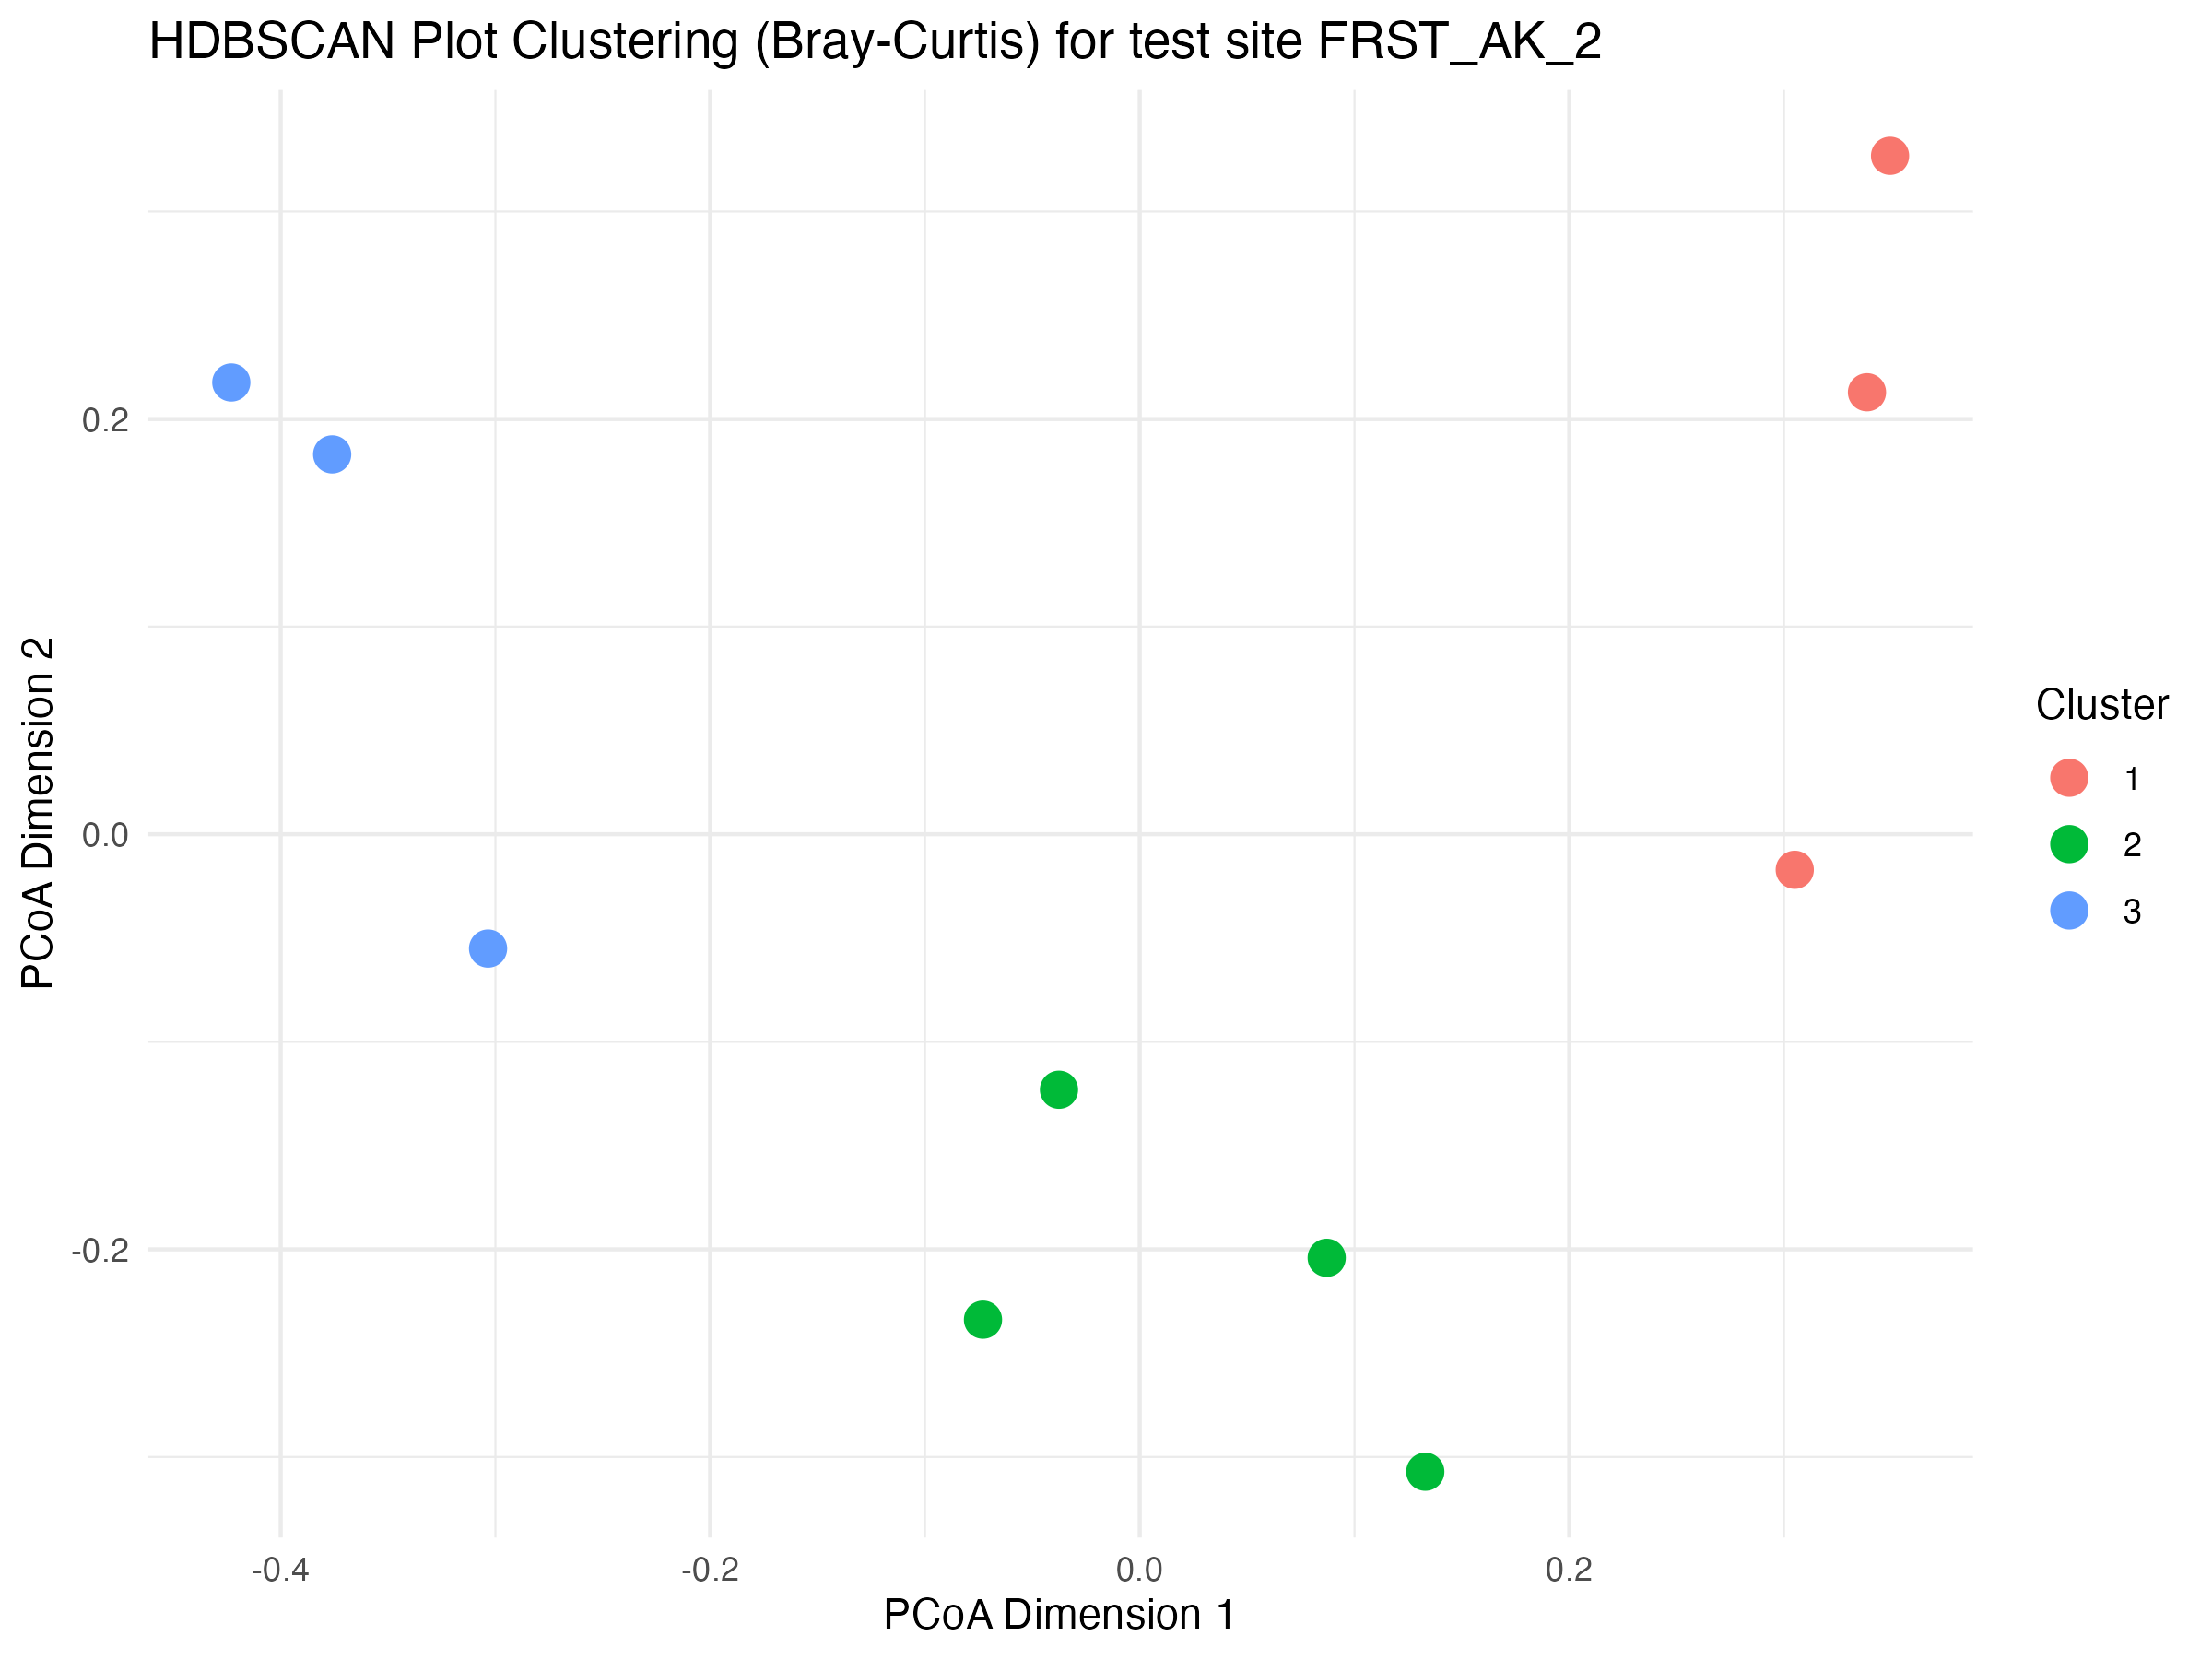
\includegraphics[width=0.9\textwidth]{Figures/Appendix/PlantCommunityClustering/FRST_AK_2_HDBSCAN_clusters.png} % Replace with your actual image path
    \caption{Community cluster HDBSCAN plot for test site FRST\_AK\_2}
    \label{fig:FRST_AK_2_HDBSCAN_clusters}
\end{figure}

\begin{figure}[H]
    \centering
    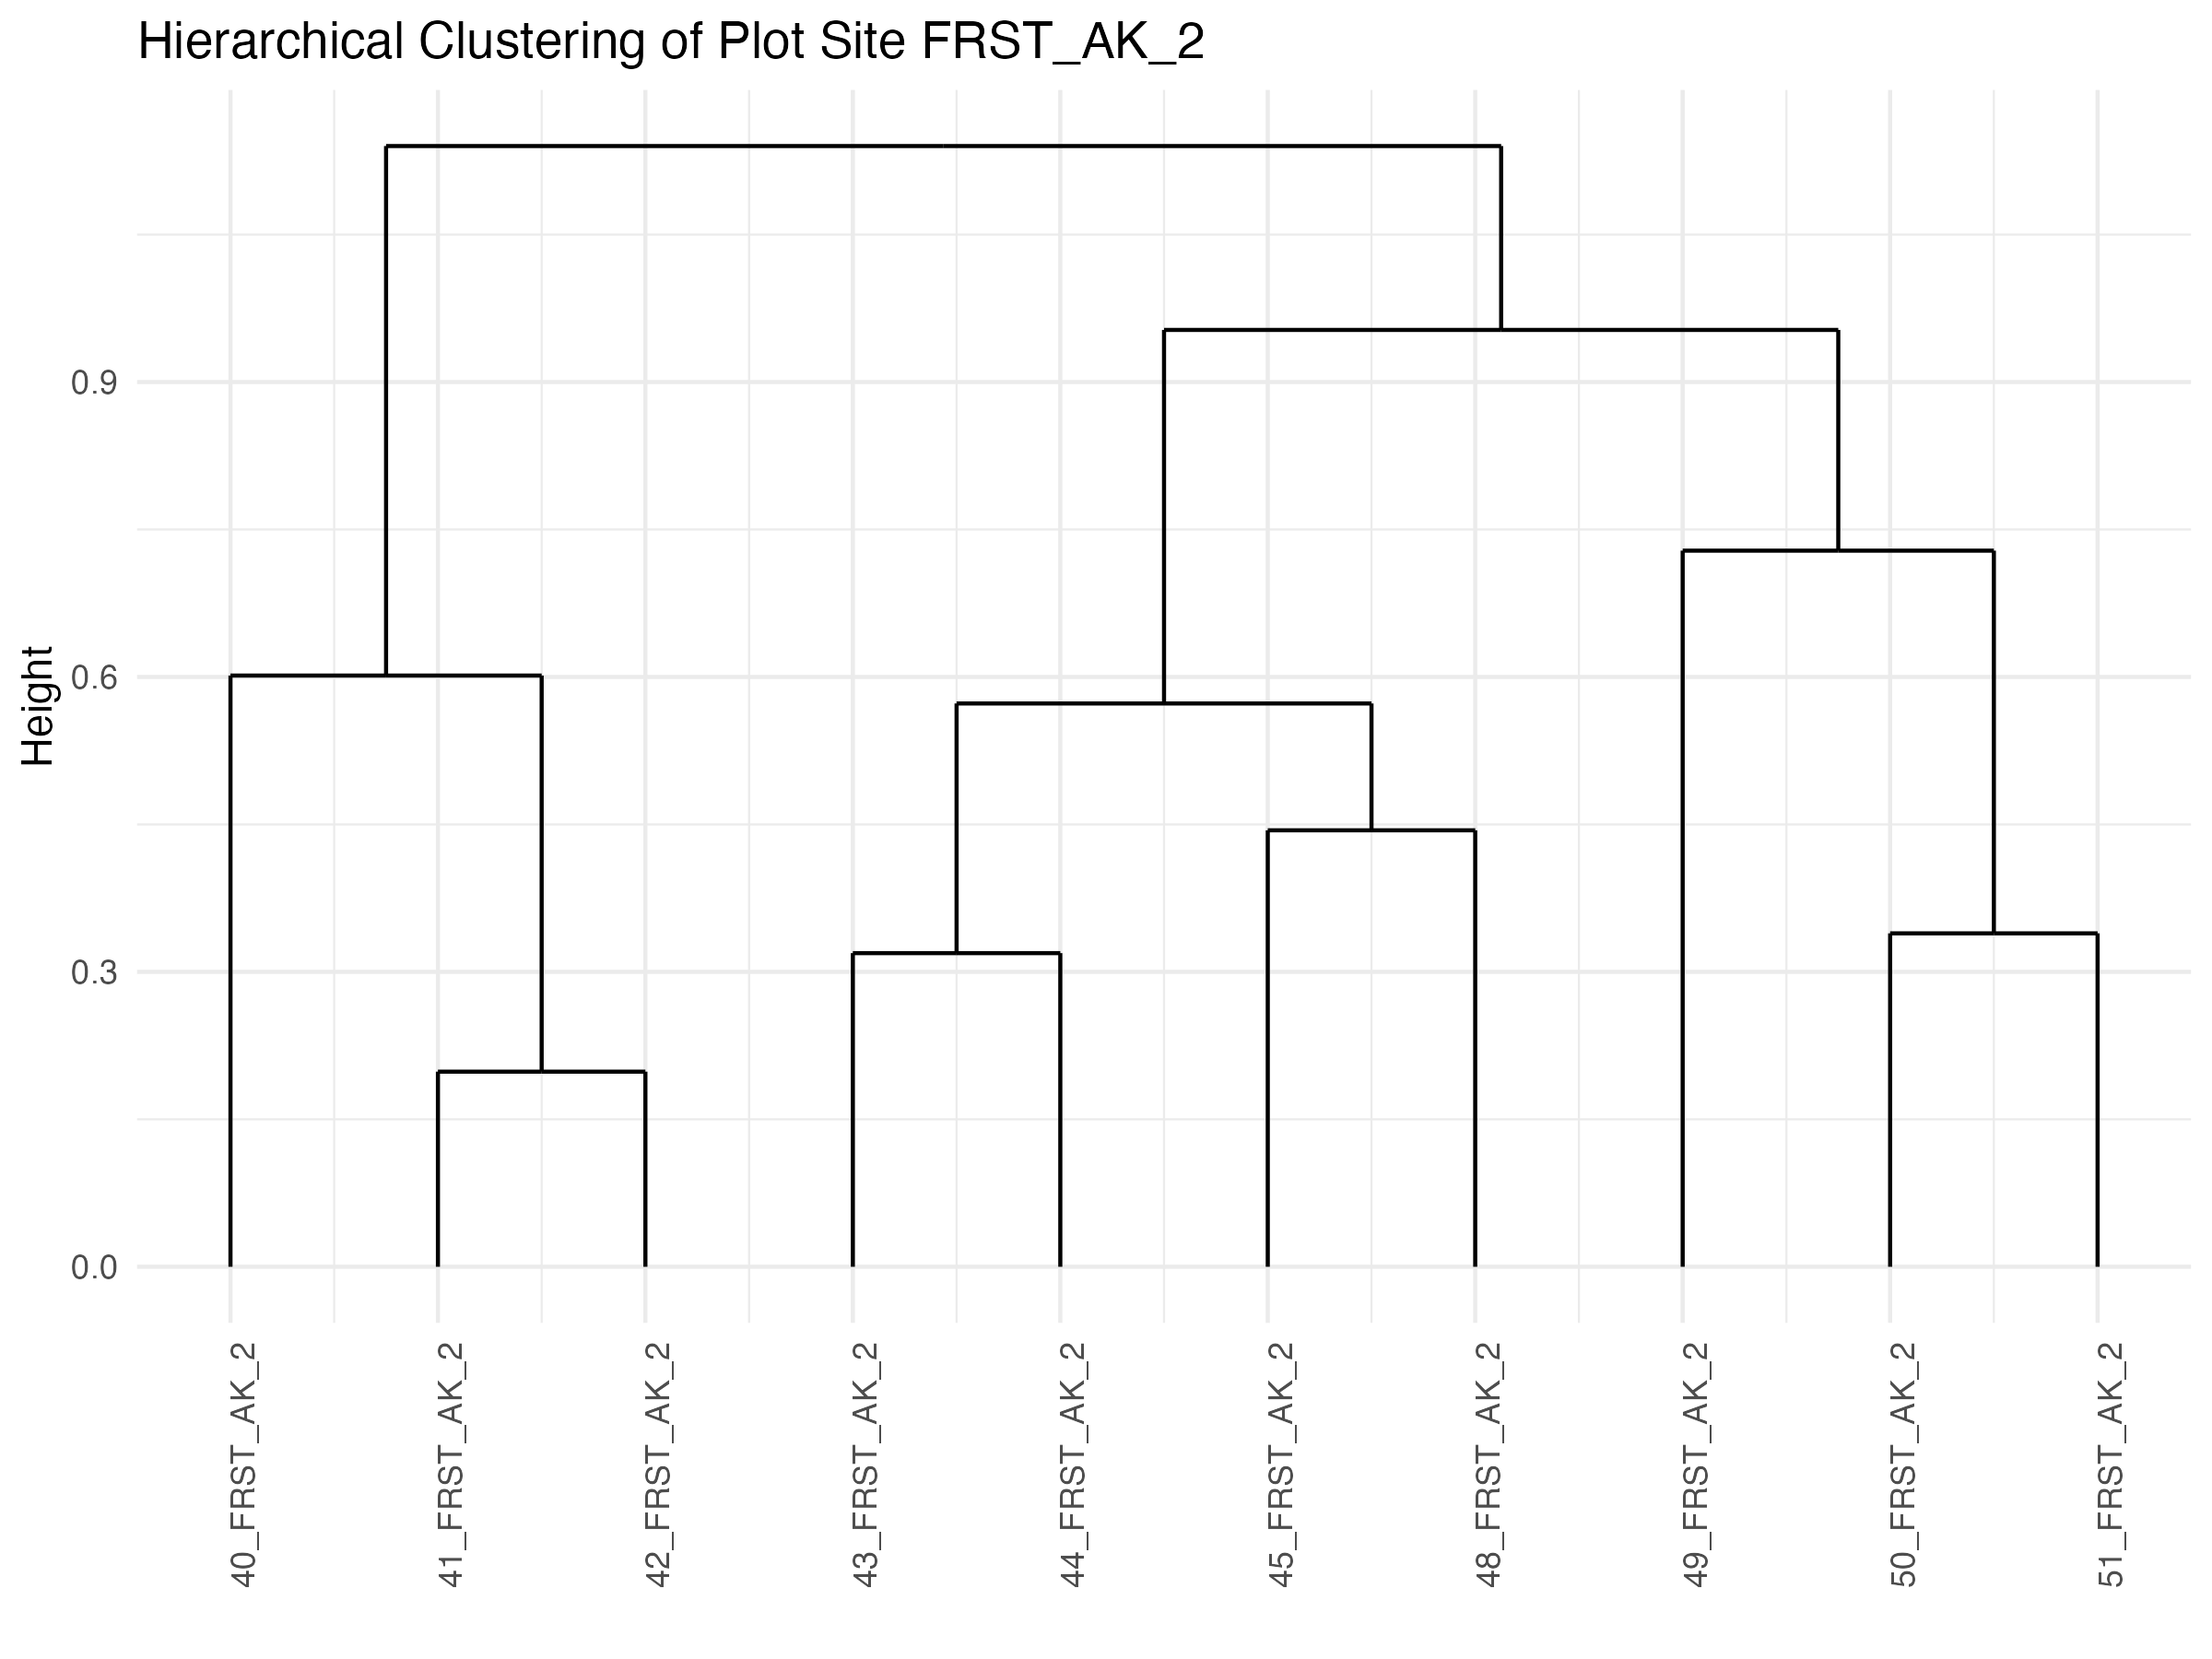
\includegraphics[width=0.9\textwidth]{Figures/Appendix/PlantCommunityClustering/FRST_AK_2_DENDRO.png} % Replace with your actual image path
    \caption{Community cluster dendrogram plot for test site FRST\_AK\_2}
    \label{fig:FRST_AK_2_DENDRO}
\end{figure}

\subsection{FRST\_AK\_3}
\begin{figure}[H]
    \centering
    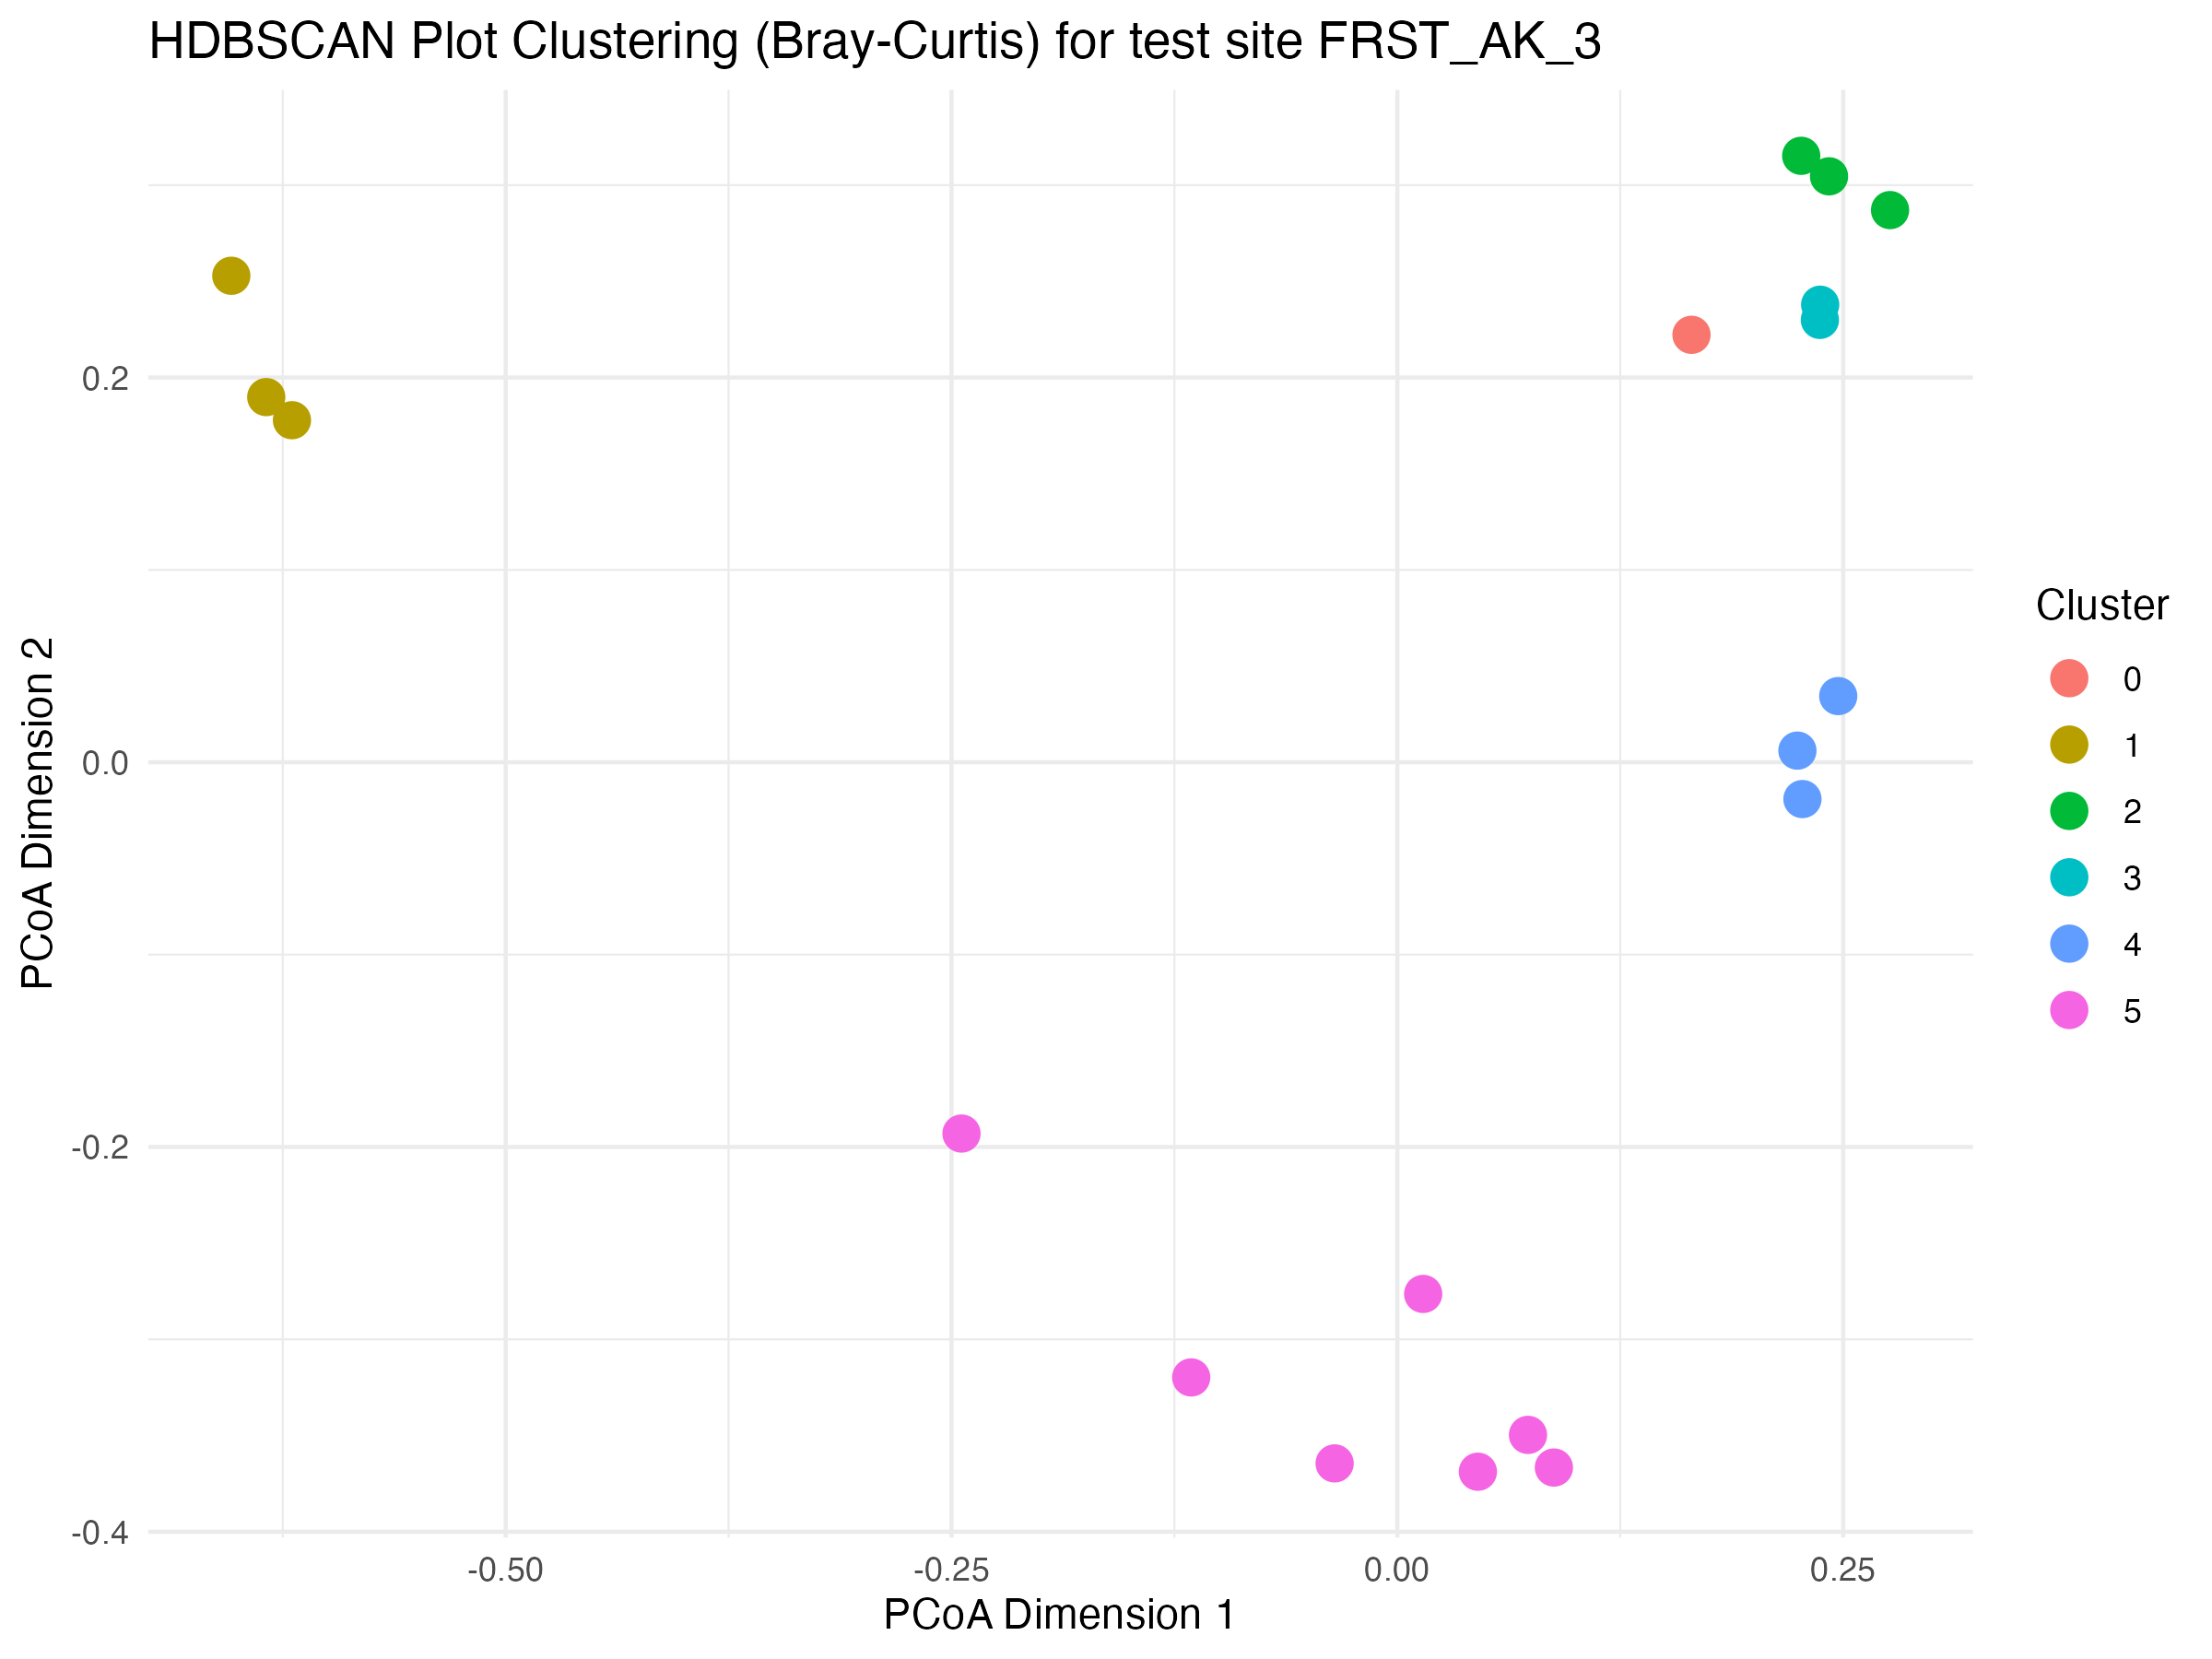
\includegraphics[width=0.9\textwidth]{Figures/Appendix/PlantCommunityClustering/FRST_AK_3_HDBSCAN_clusters.png} % Replace with your actual image path
    \caption{Community cluster HDBSCAN plot for test site FRST\_AK\_3}
    \label{fig:FRST_AK_3_HDBSCAN_clusters}
\end{figure}

\begin{figure}[H]
    \centering
    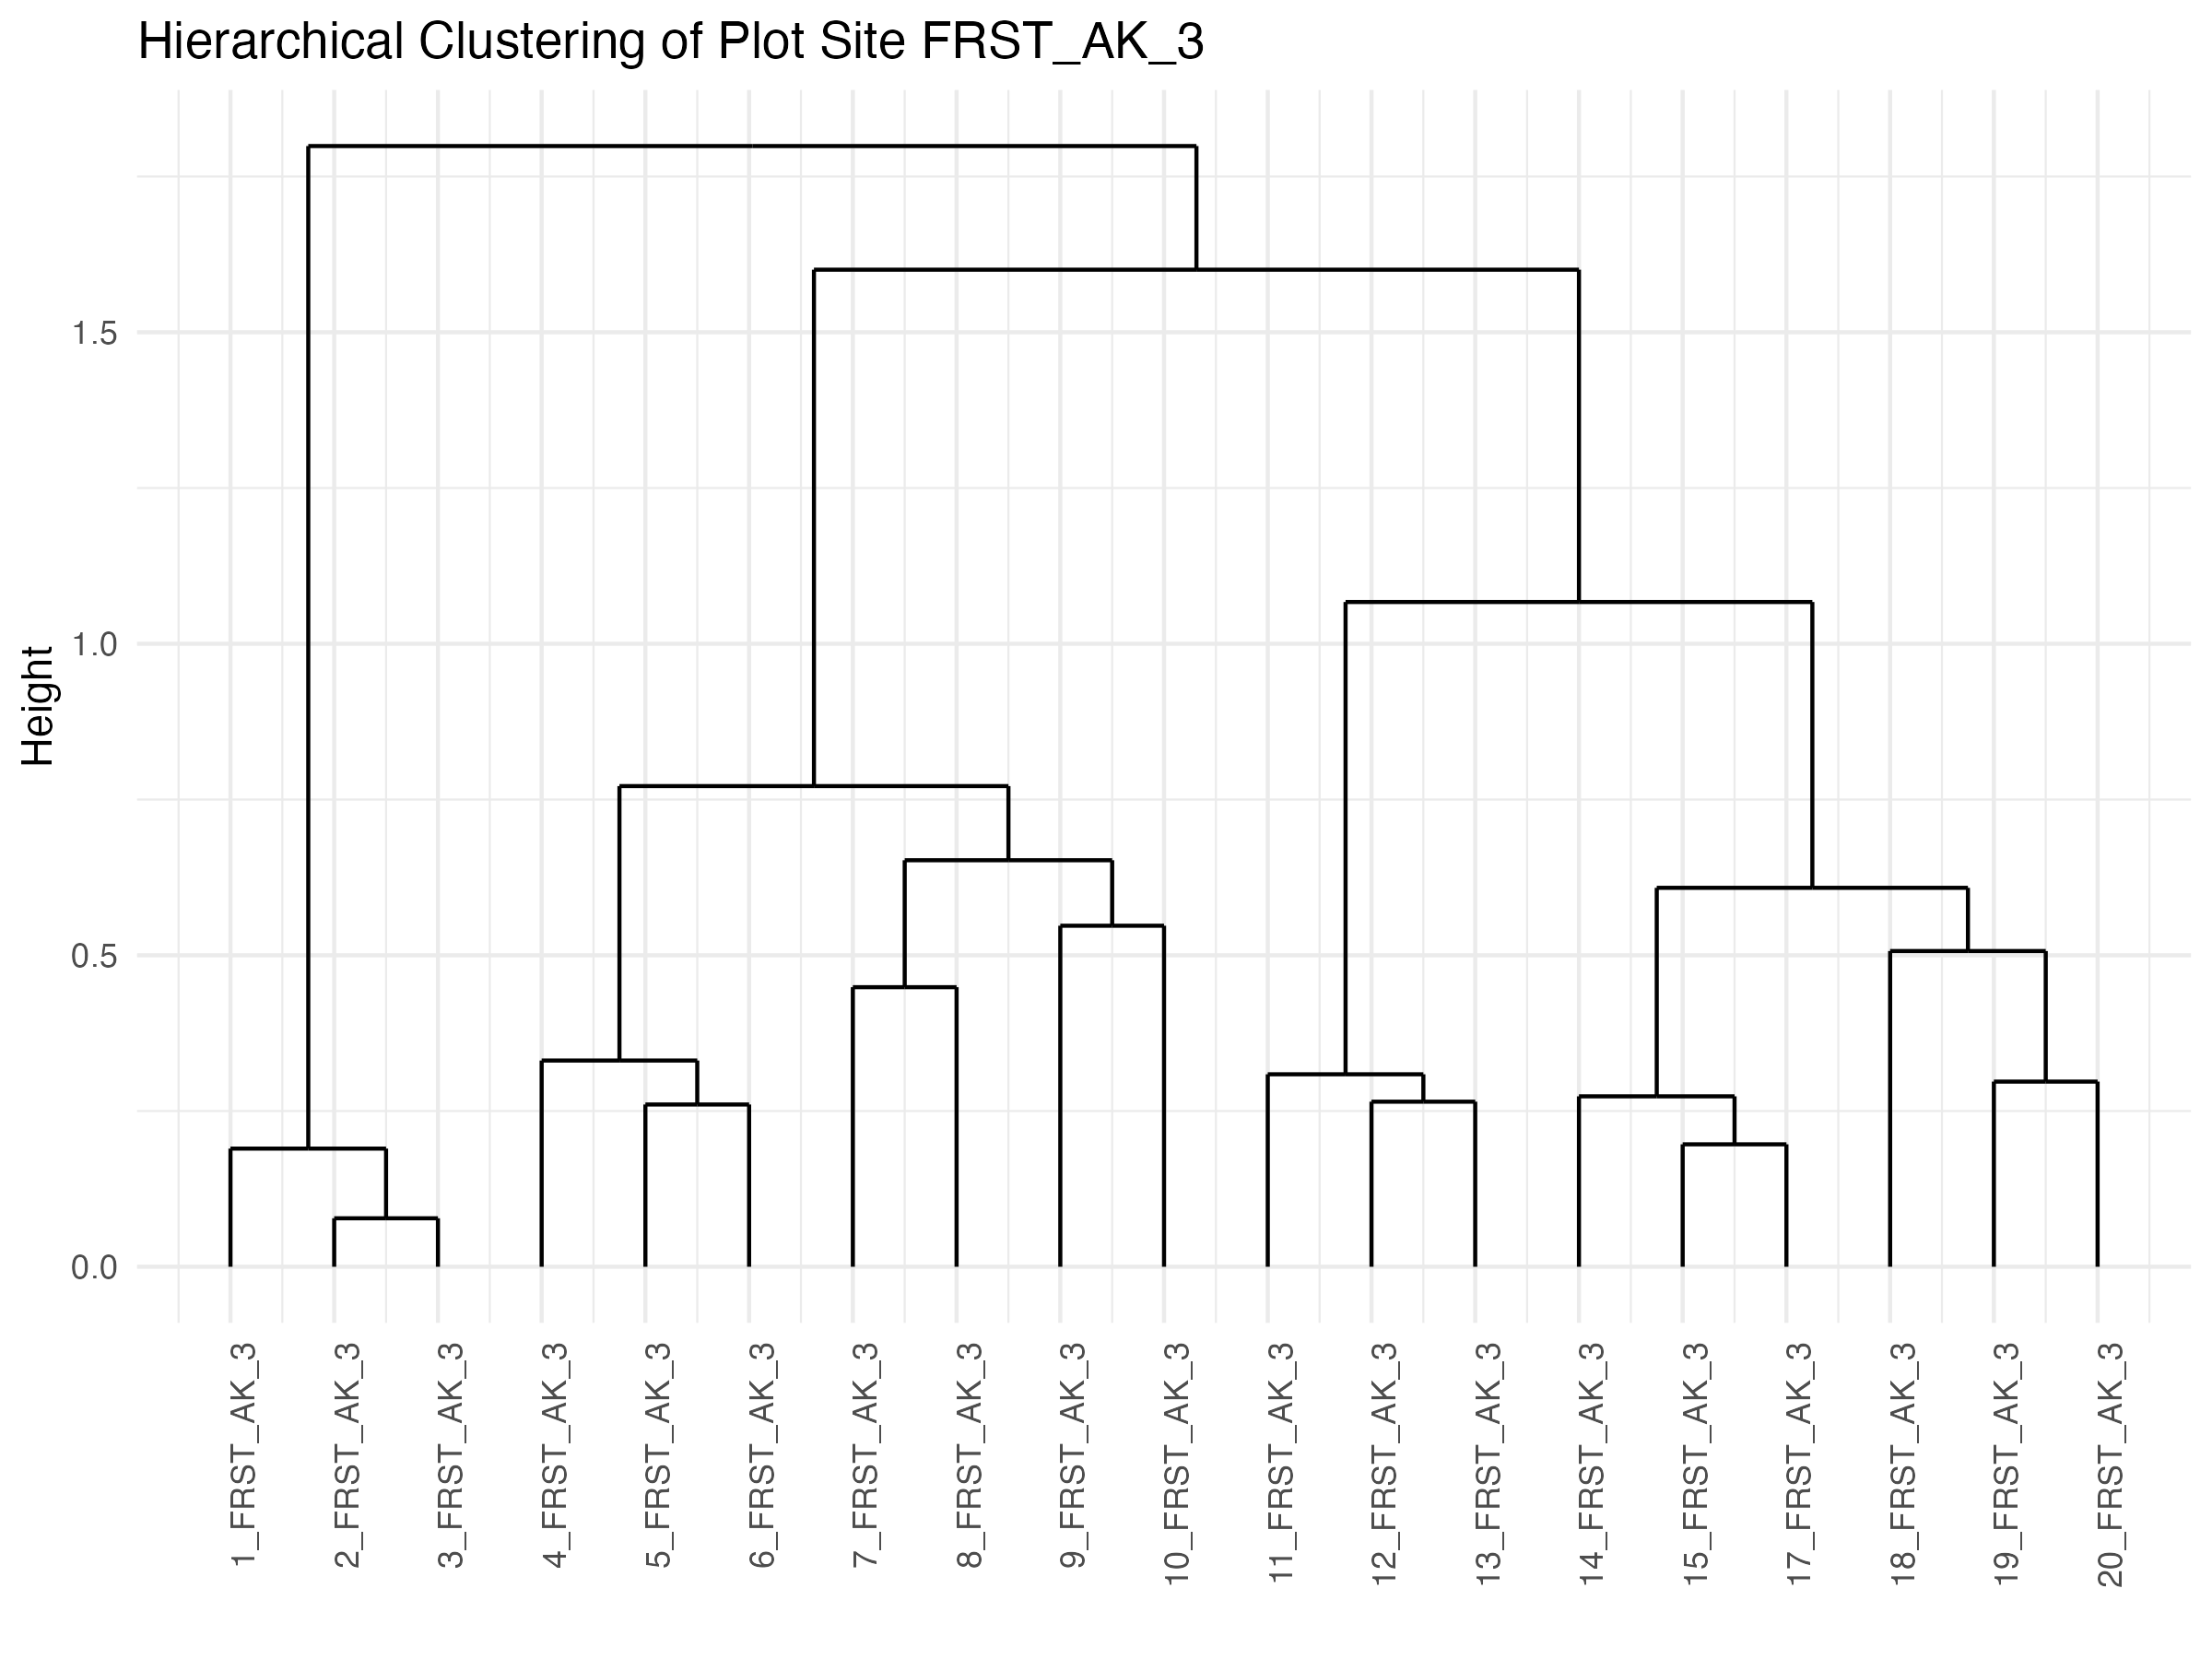
\includegraphics[width=0.9\textwidth]{Figures/Appendix/PlantCommunityClustering/FRST_AK_3_DENDRO.png} % Replace with your actual image path
    \caption{Community cluster dendrogram plot for test site FRST\_AK\_3}
    \label{fig:FRST_AK_3_DENDRO}
\end{figure}

\subsection{PRUAIR\_DW\_1}
\begin{figure}[H]
    \centering
    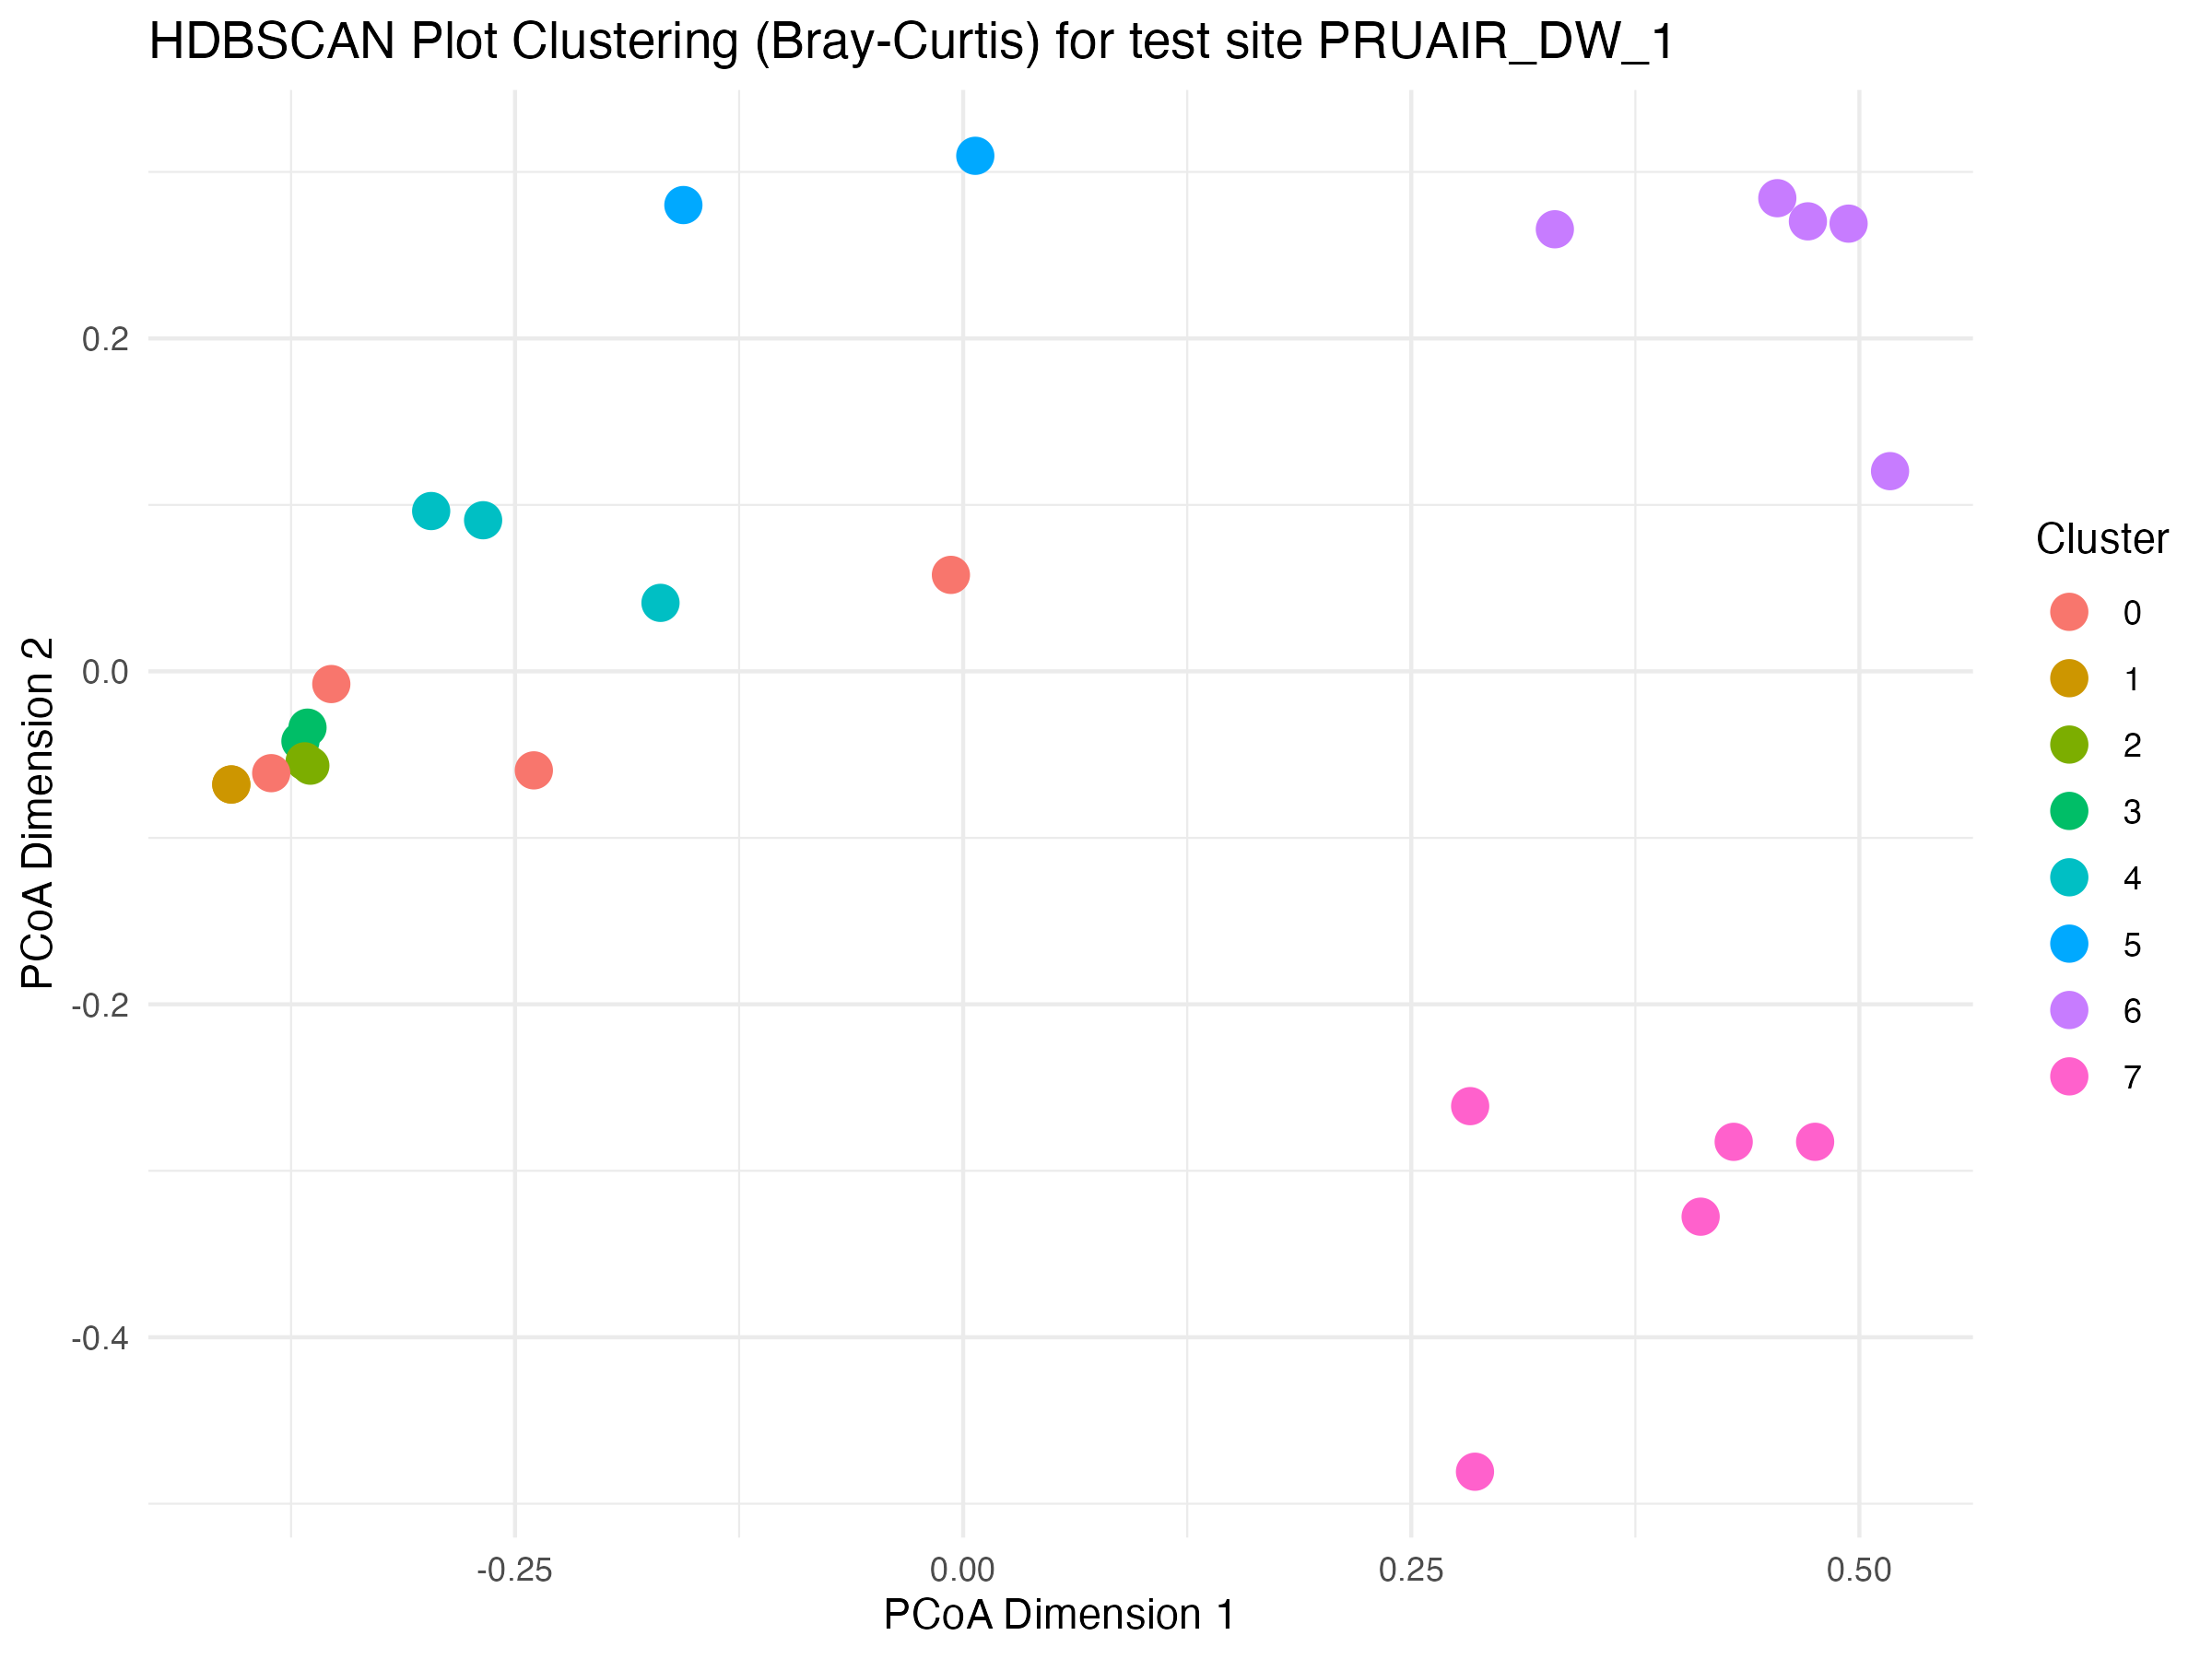
\includegraphics[width=0.9\textwidth]{Figures/Appendix/PlantCommunityClustering/PRUAIR_DW_1_HDBSCAN_clusters.png} % Replace with your actual image path
    \caption{Community cluster HDBSCAN plot for test site PRUAIR\_DW\_1}
    \label{fig:PRUAIR_DW_1_HDBSCAN_clusters}
\end{figure}

\begin{figure}[H]
    \centering
    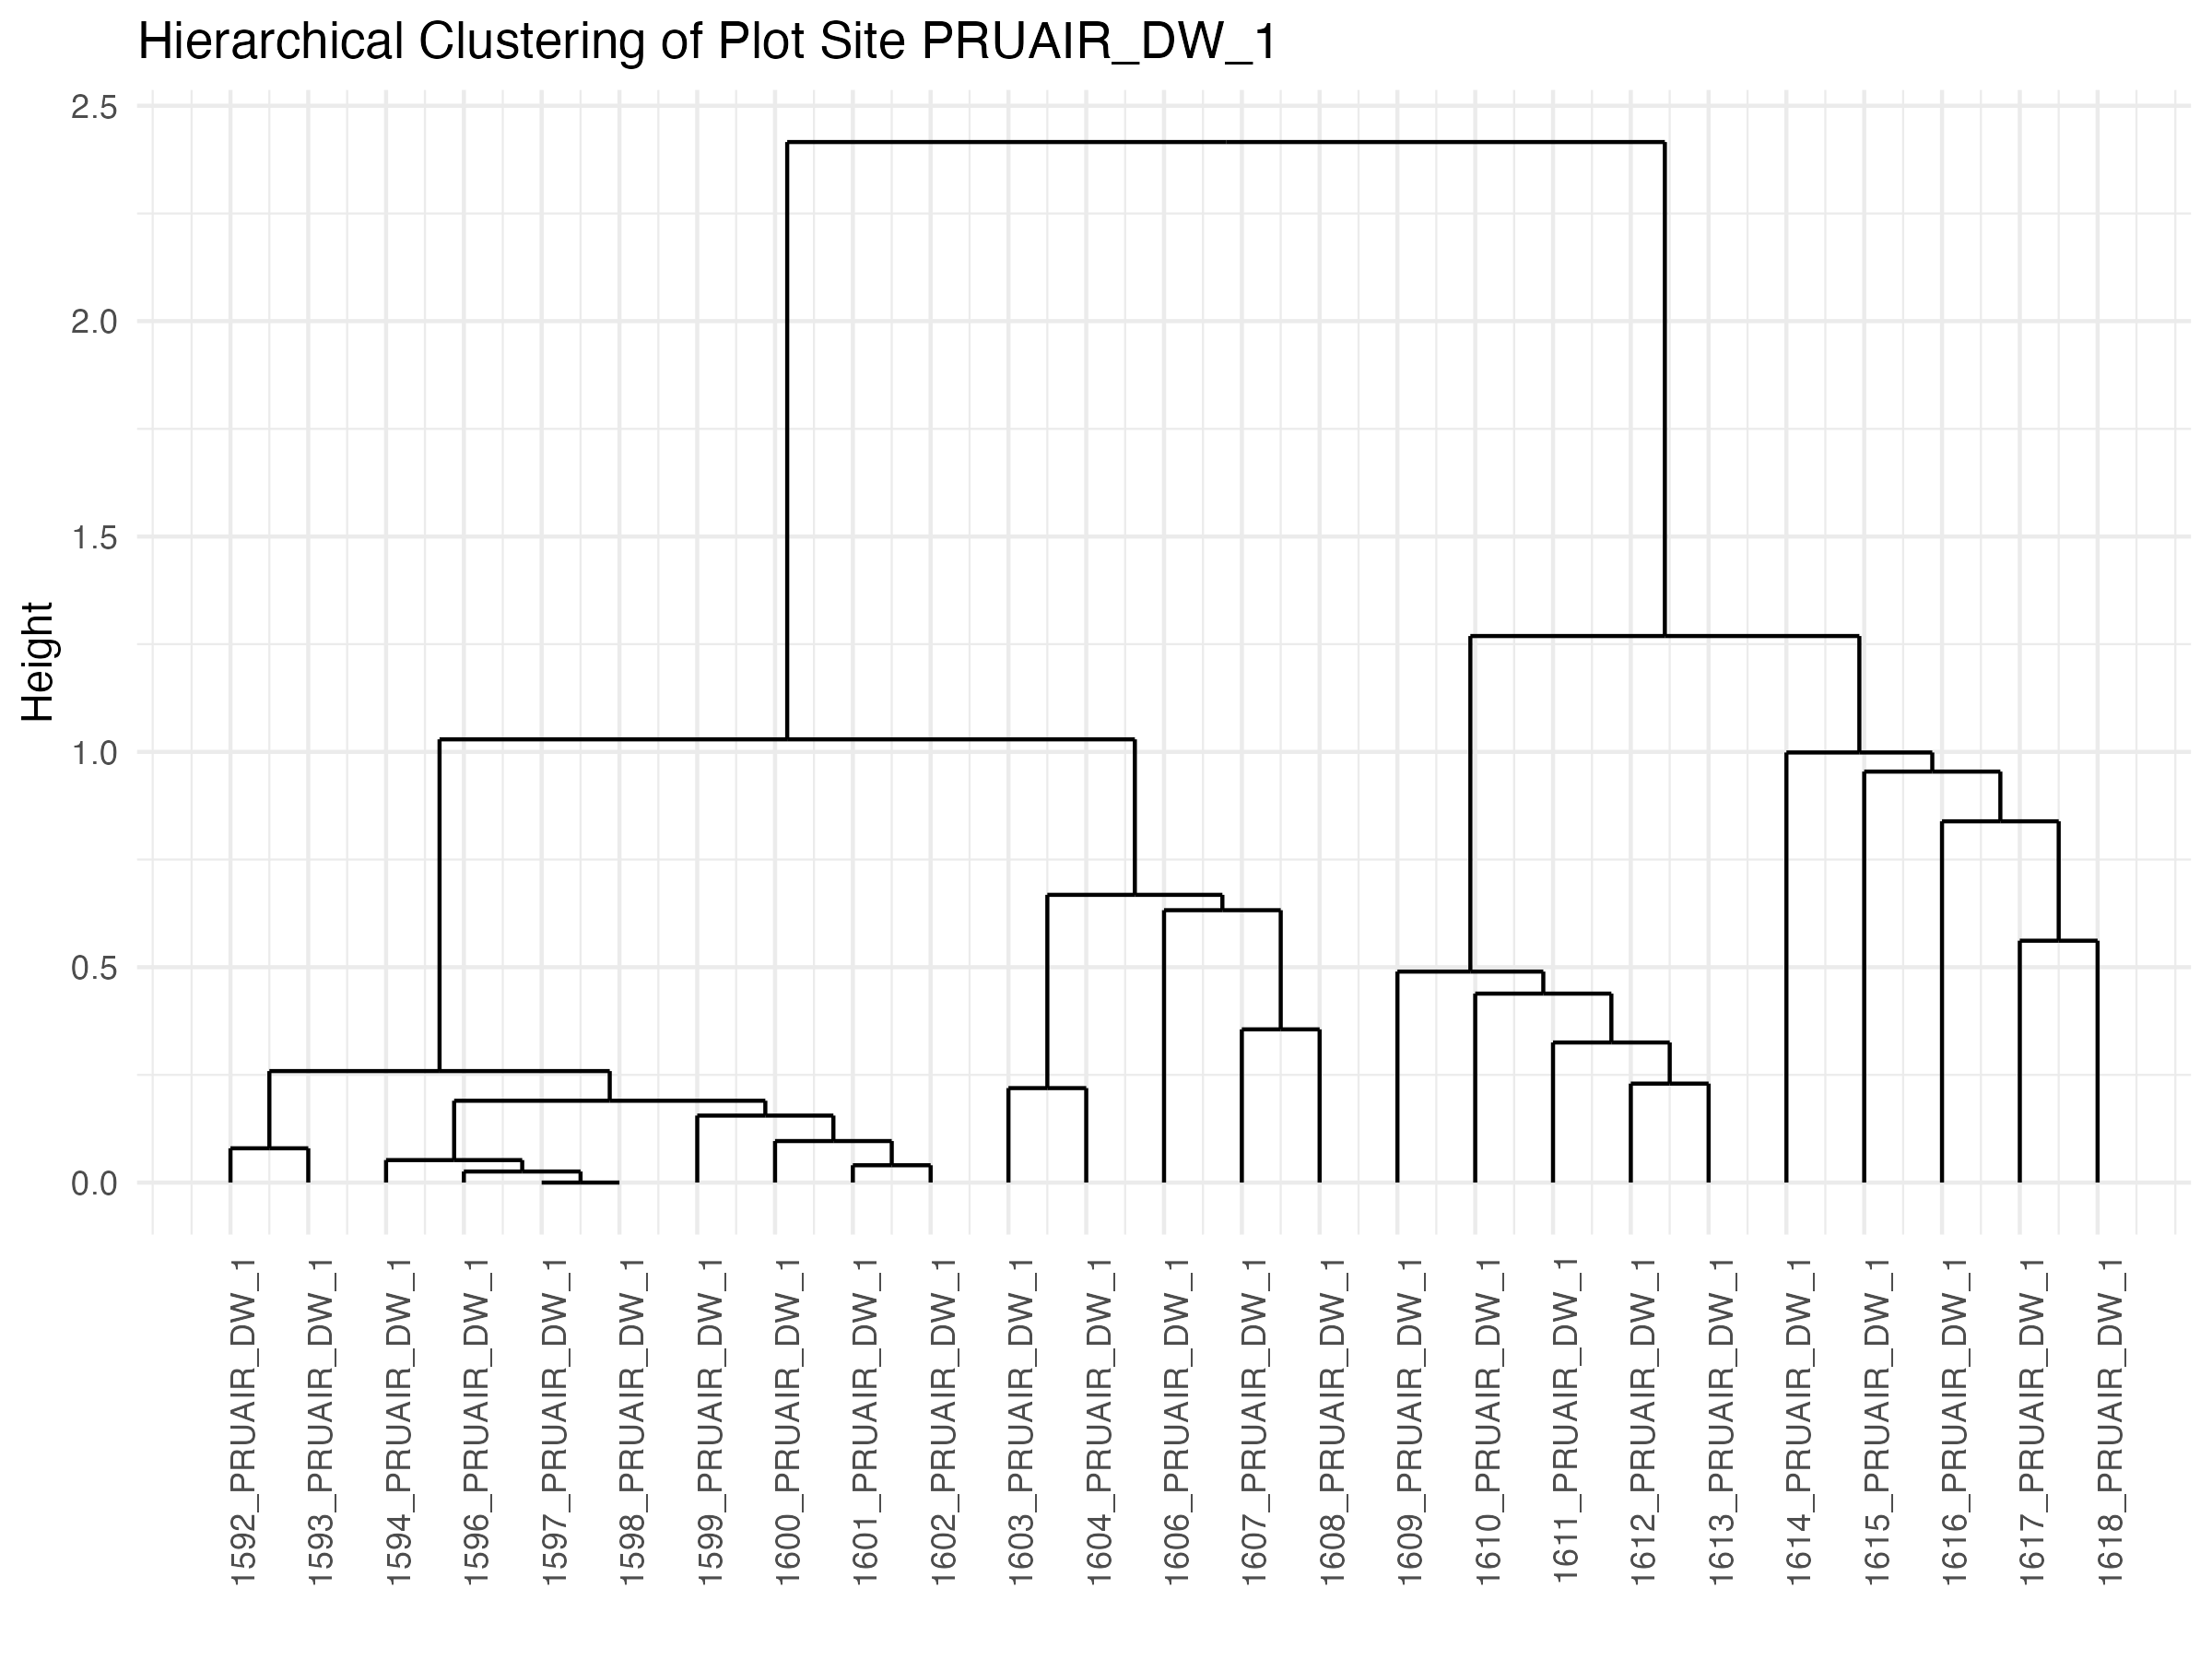
\includegraphics[width=0.9\textwidth]{Figures/Appendix/PlantCommunityClustering/PRUAIR_DW_1_DENDRO.png} % Replace with your actual image path
    \caption{Community cluster dendrogram plot for test site PRUAIR\_DW\_1}
    \label{fig:PRUAIR_DW_1_DENDRO}
\end{figure}

\subsection{PRUARC\_DW\_1}
\begin{figure}[H]
    \centering
    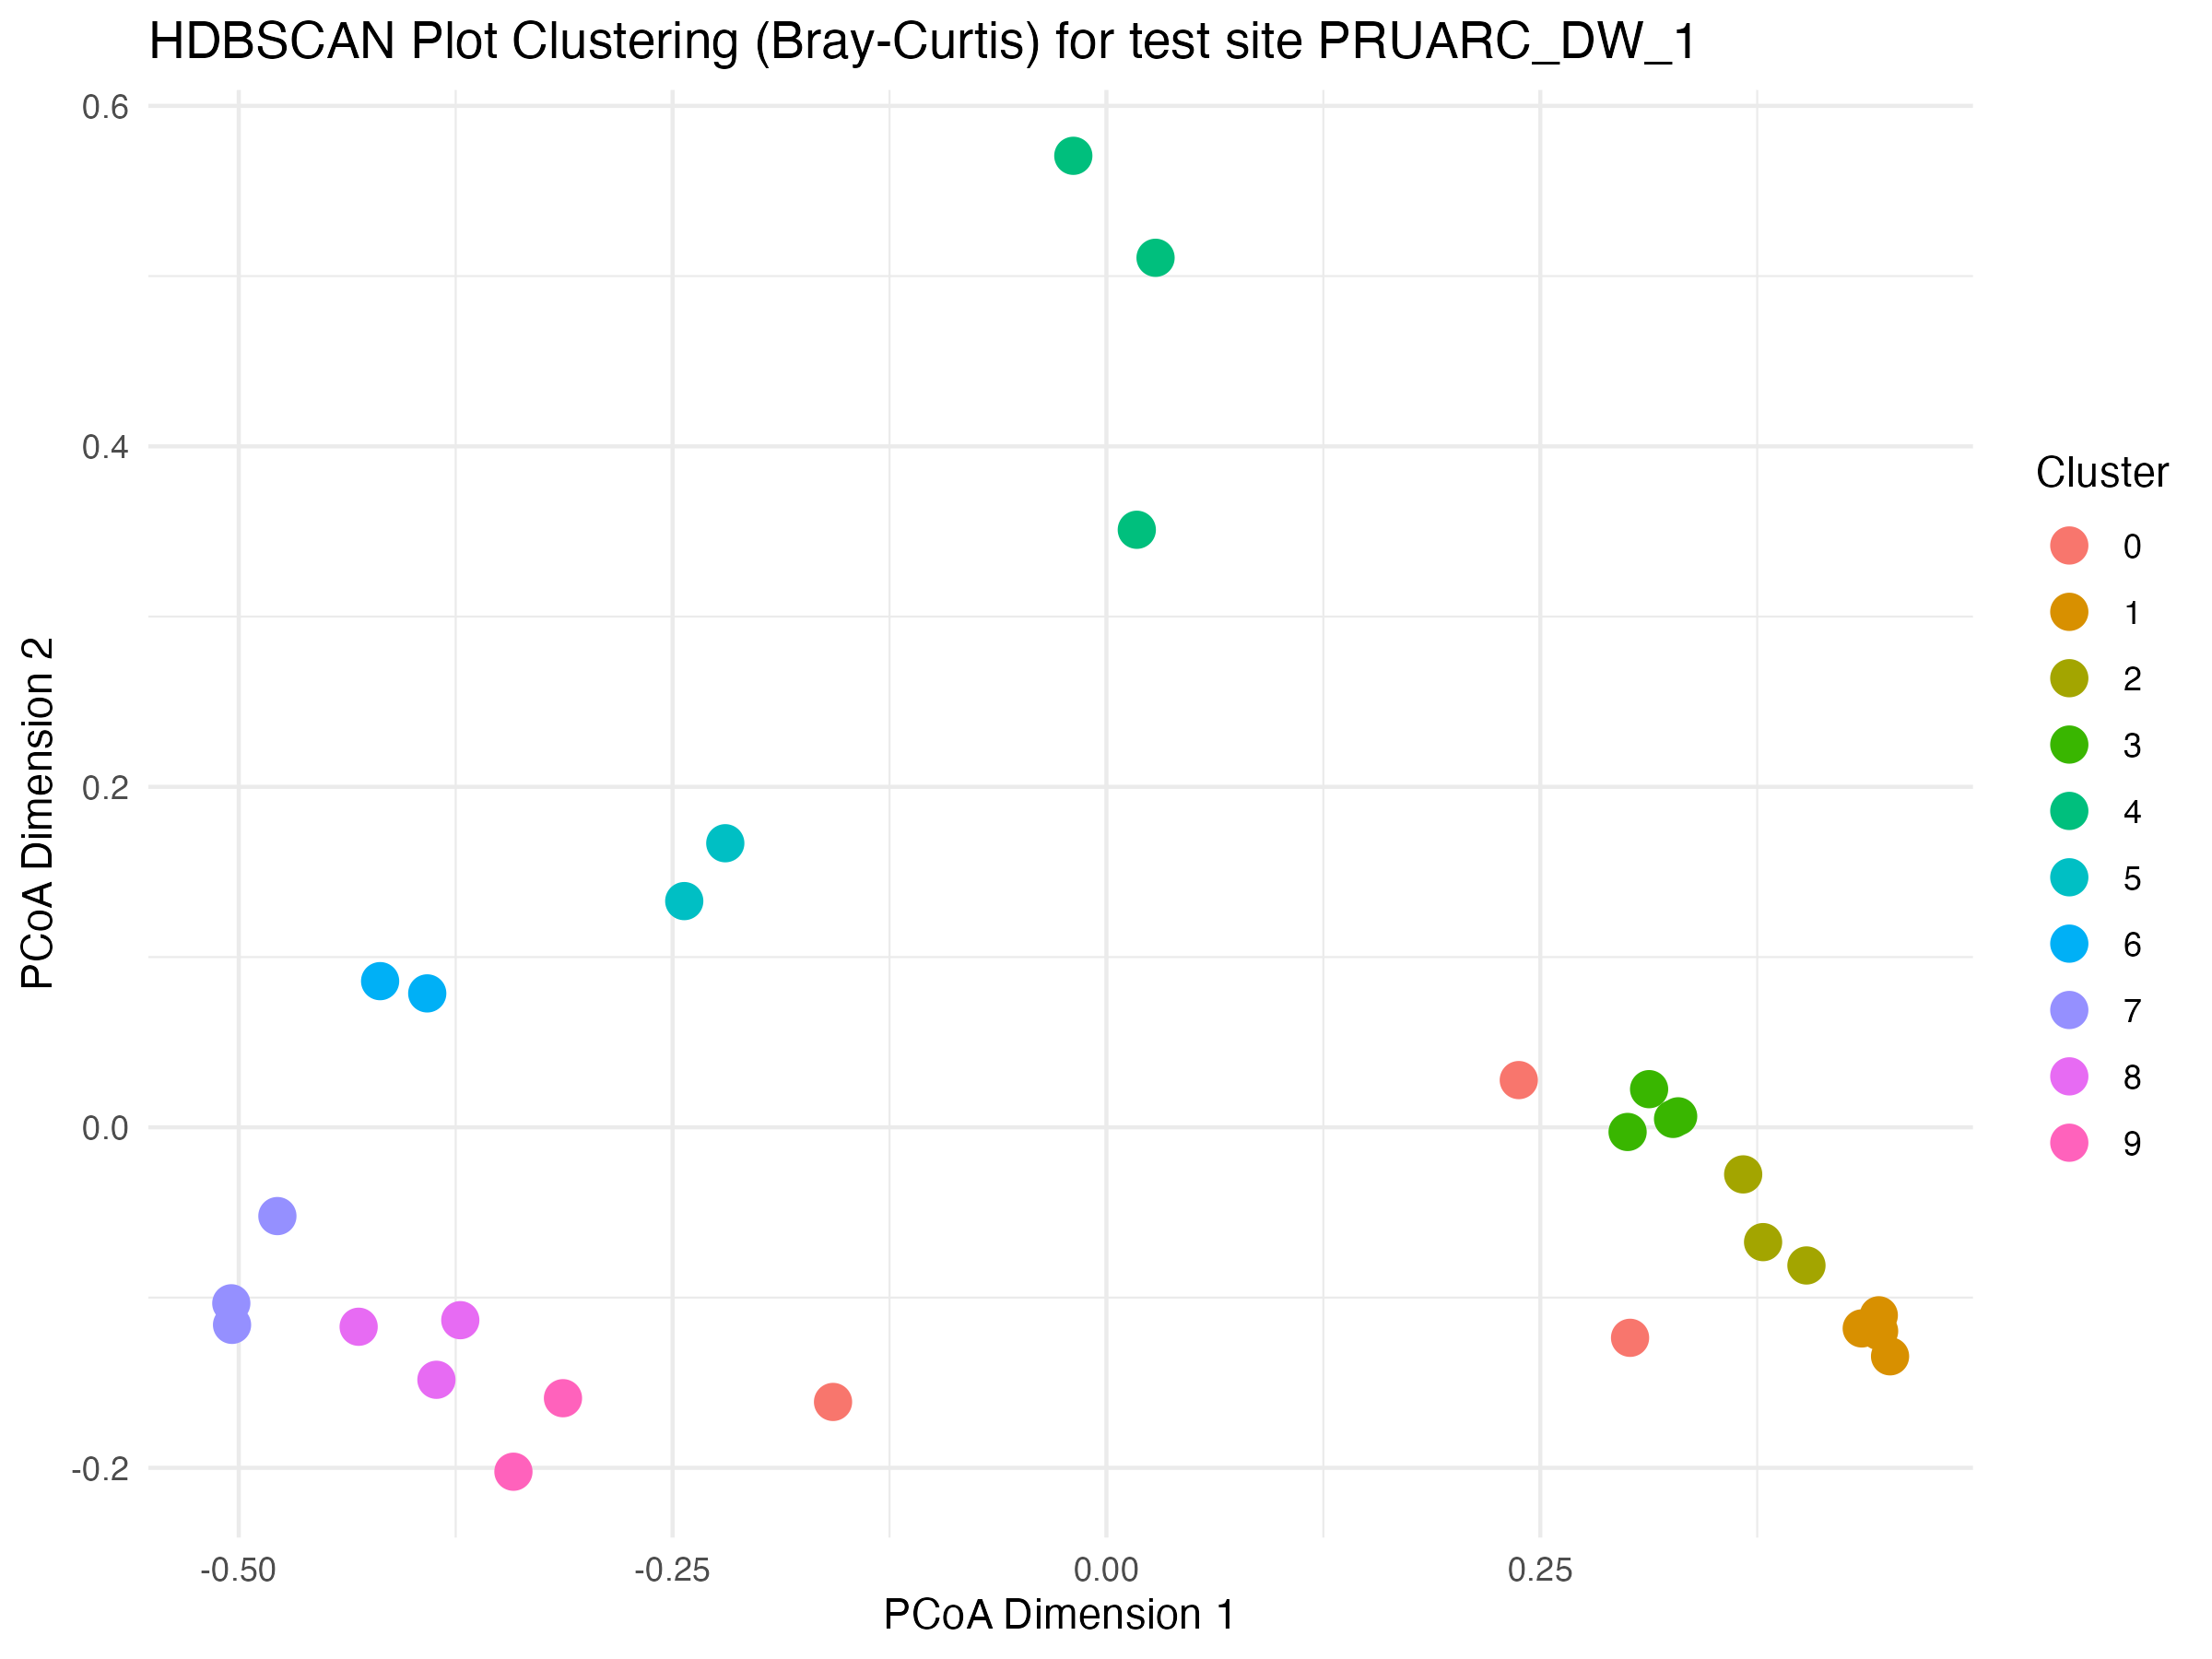
\includegraphics[width=0.9\textwidth]{Figures/Appendix/PlantCommunityClustering/PRUARC_DW_1_HDBSCAN_clusters.png} % Replace with your actual image path
    \caption{Community cluster HDBSCAN plot for test site PRUARC\_DW\_1}
    \label{fig:PRUARC_DW_1_HDBSCAN_clusters}
\end{figure}

\begin{figure}[H]
    \centering
    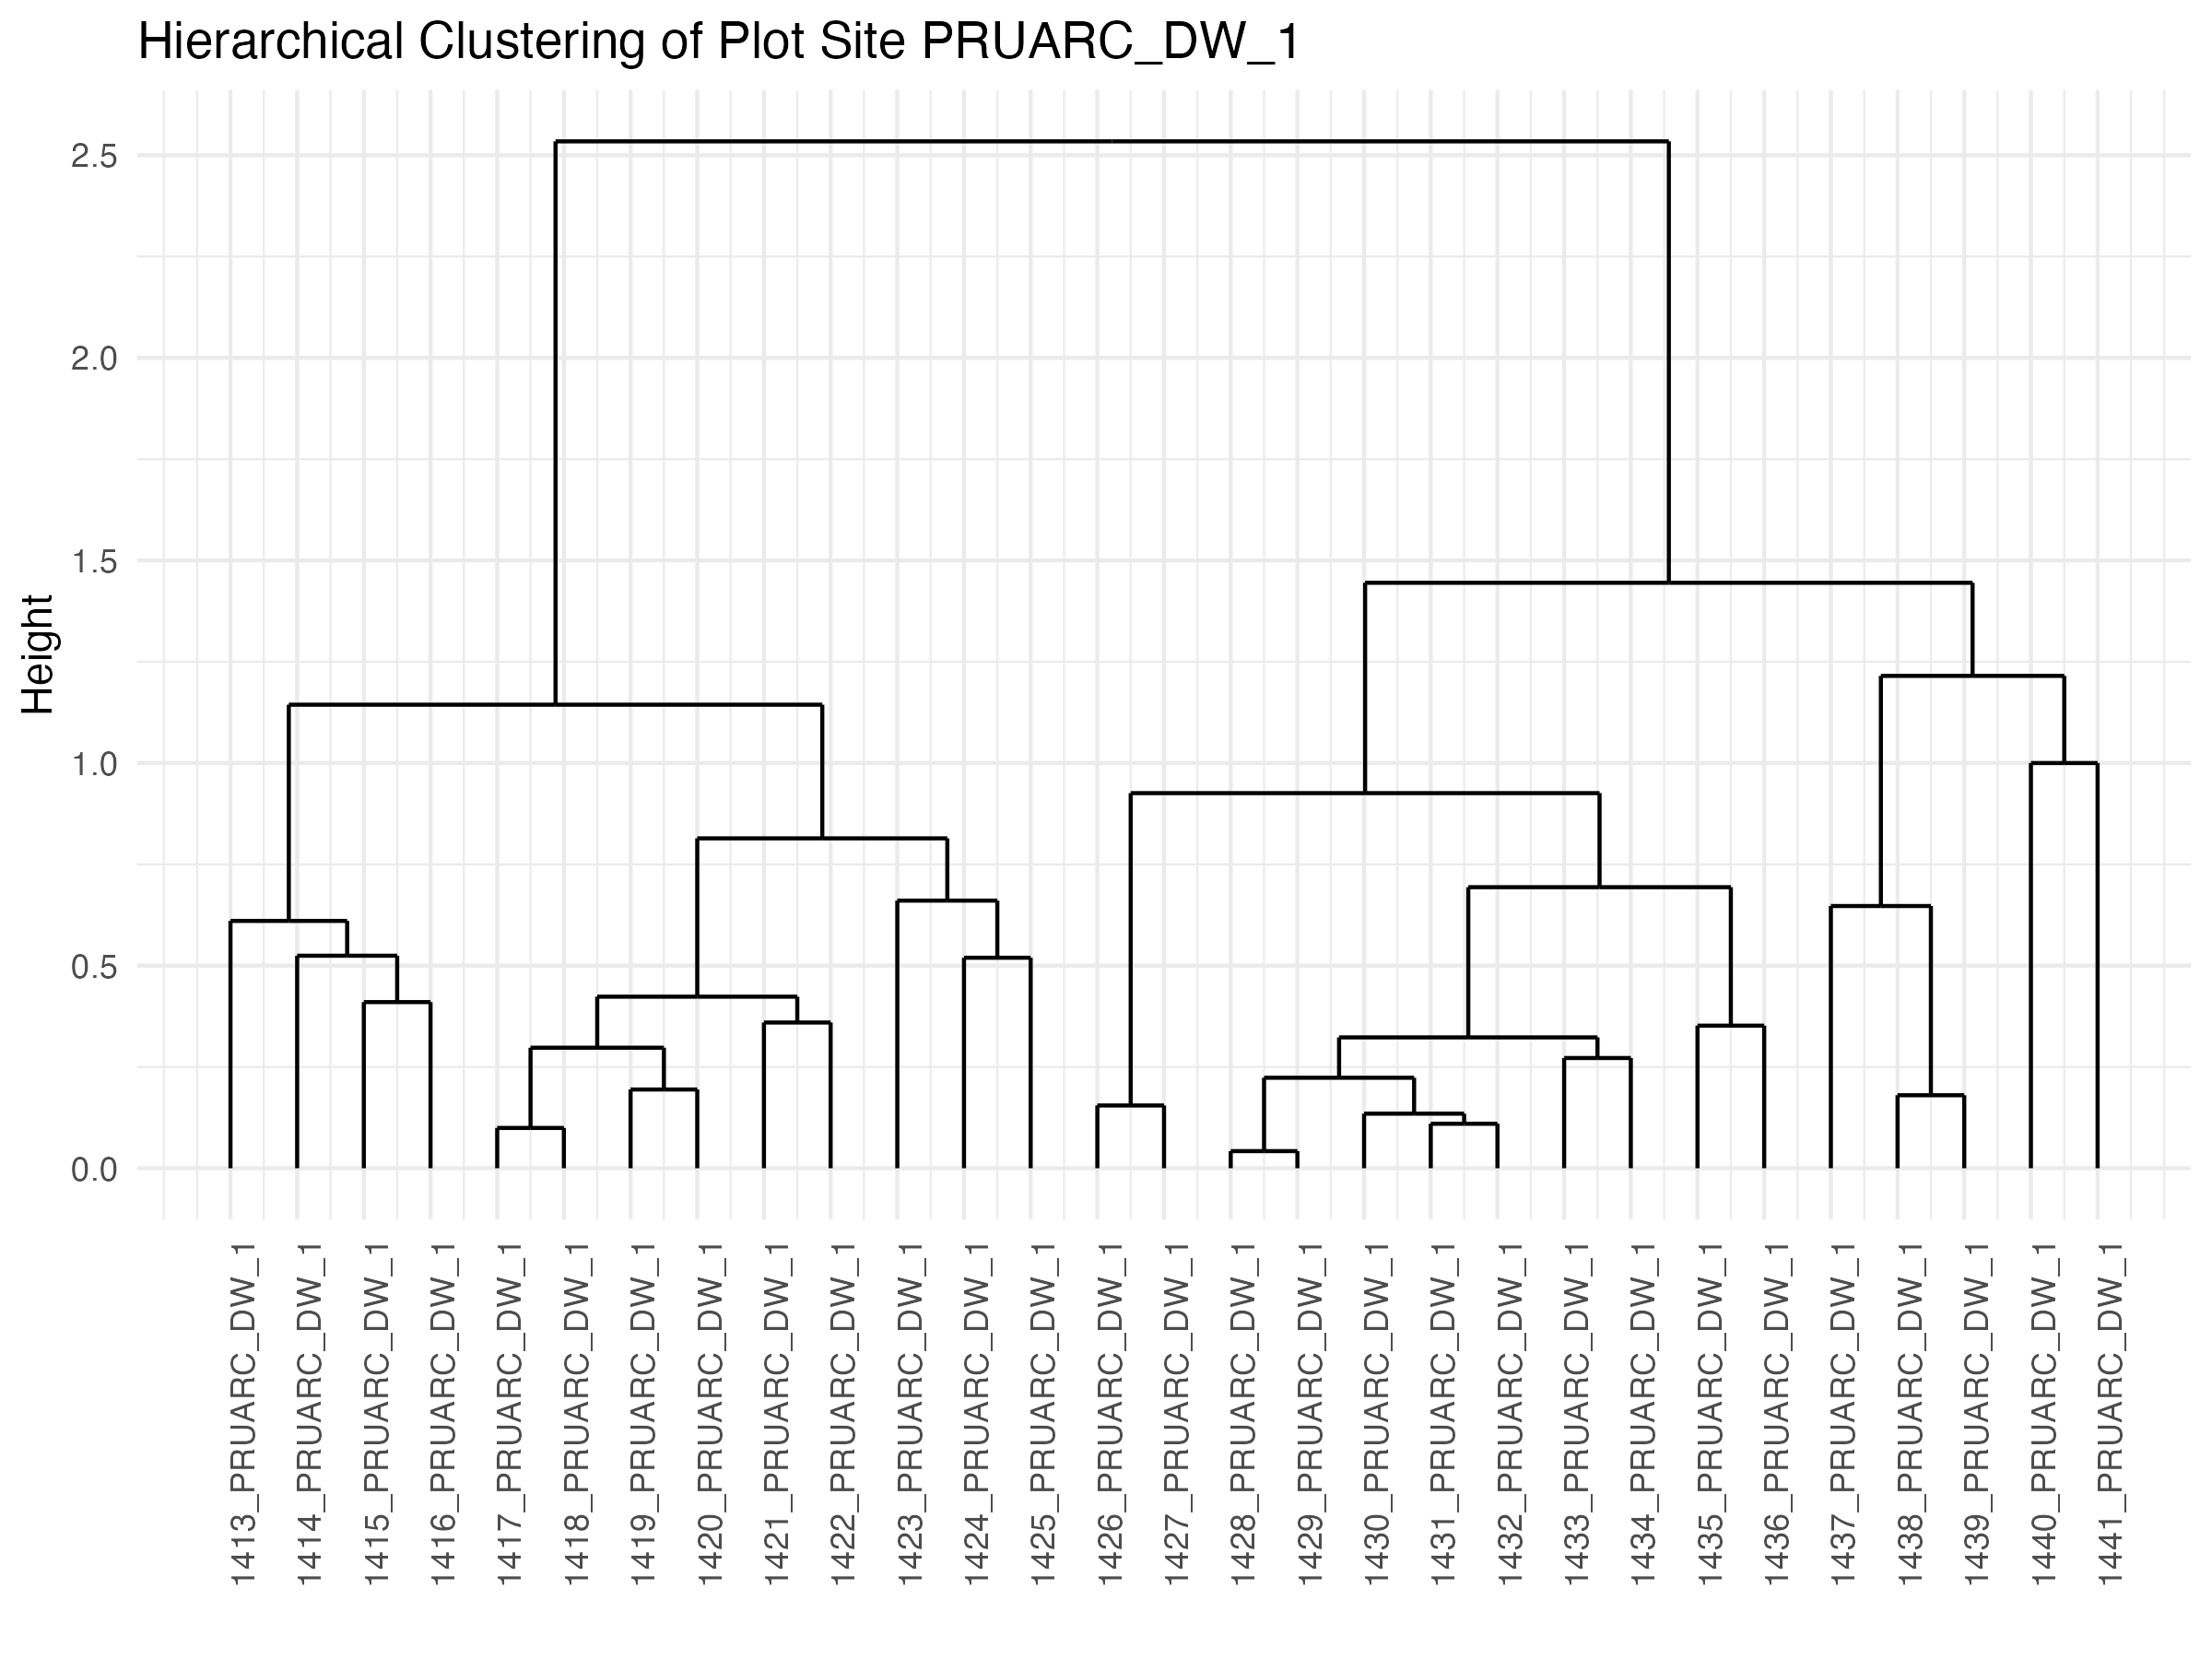
\includegraphics[width=0.9\textwidth]{Figures/Appendix/PlantCommunityClustering/PRUARC_DW_1_DENDRO.png} % Replace with your actual image path
    \caption{Community cluster dendrogram plot for test site PRUARC\_DW\_1}
    \label{fig:PRUARC_DW_1_DENDRO}
\end{figure}





% \subsection{Hugo}
% % Group 1 of 4
% \begin{figure}[H]
%     \centering
%     \begin{minipage}[b]{0.45\textwidth}
%         \centering
%         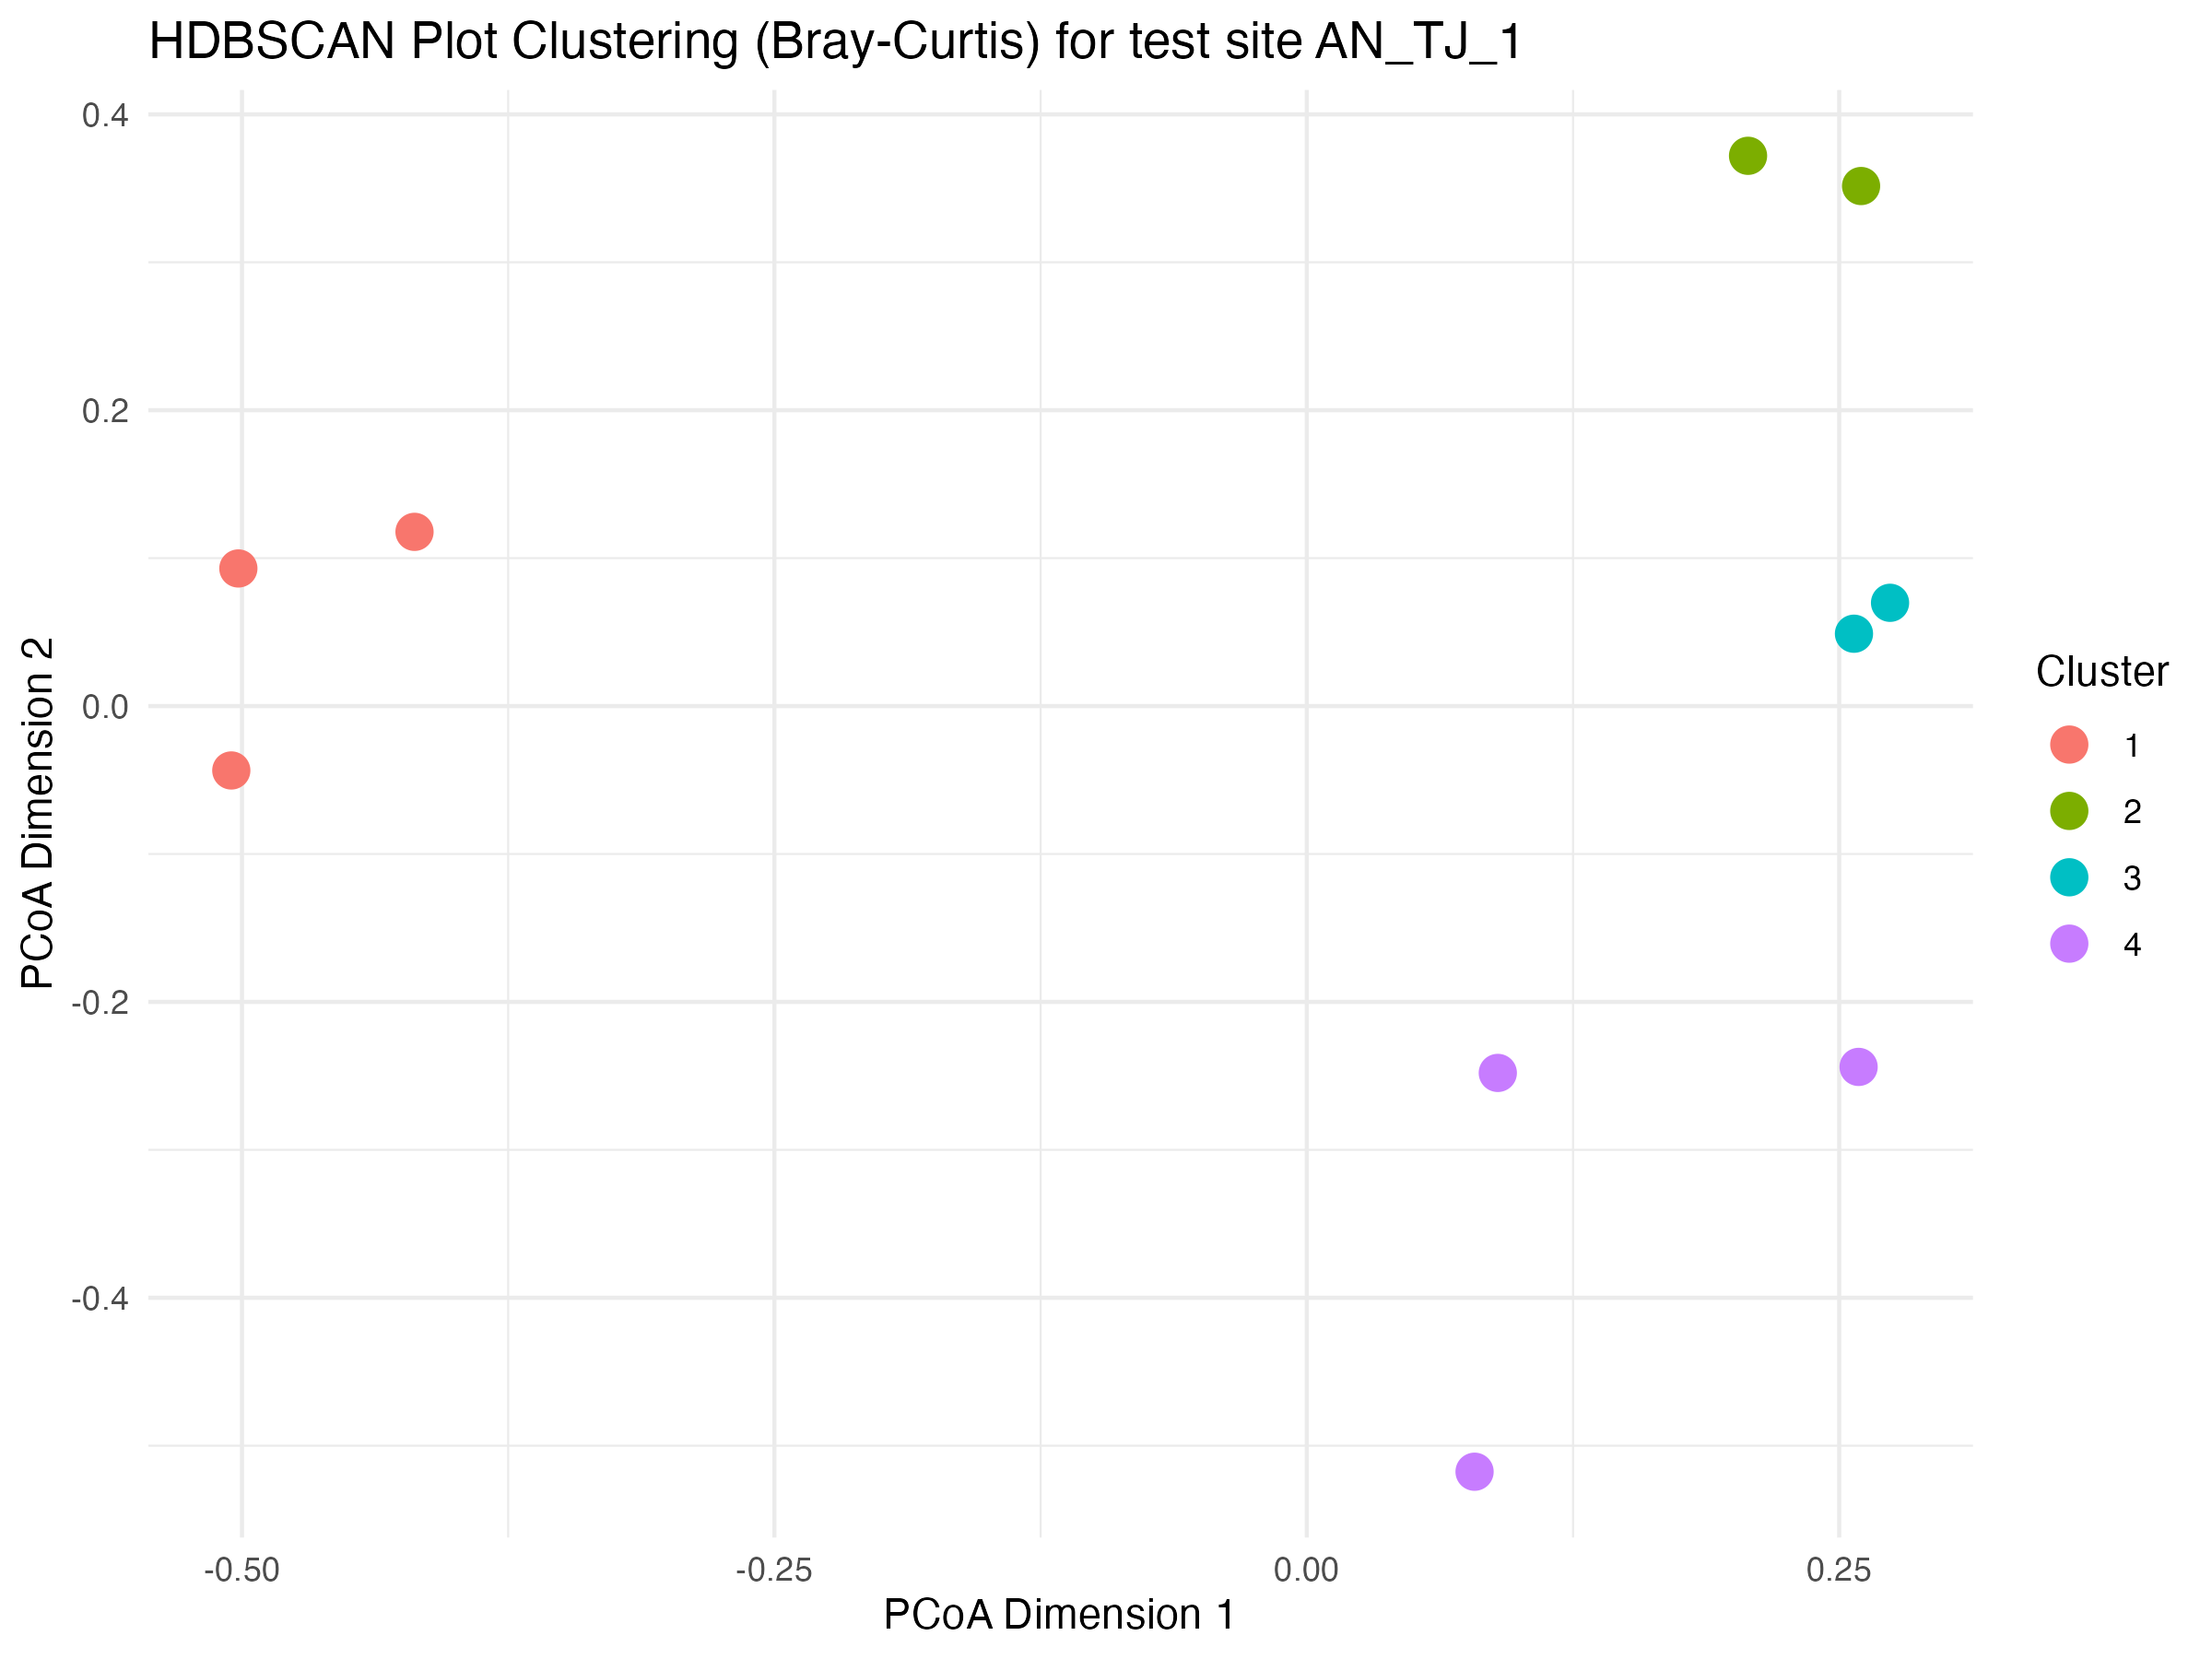
\includegraphics[width=\textwidth]{Figures/Appendix/PlantCommunityClustering/AN_TJ_1_HDBSCAN_clusters.png}
%         \caption{AN\_TJ\_1}
%         \label{fig:AN_TJ_1_HDBSCAN_clusters}
%     \end{minipage}
%     \hfill
%     \begin{minipage}[b]{0.45\textwidth}
%         \centering
%         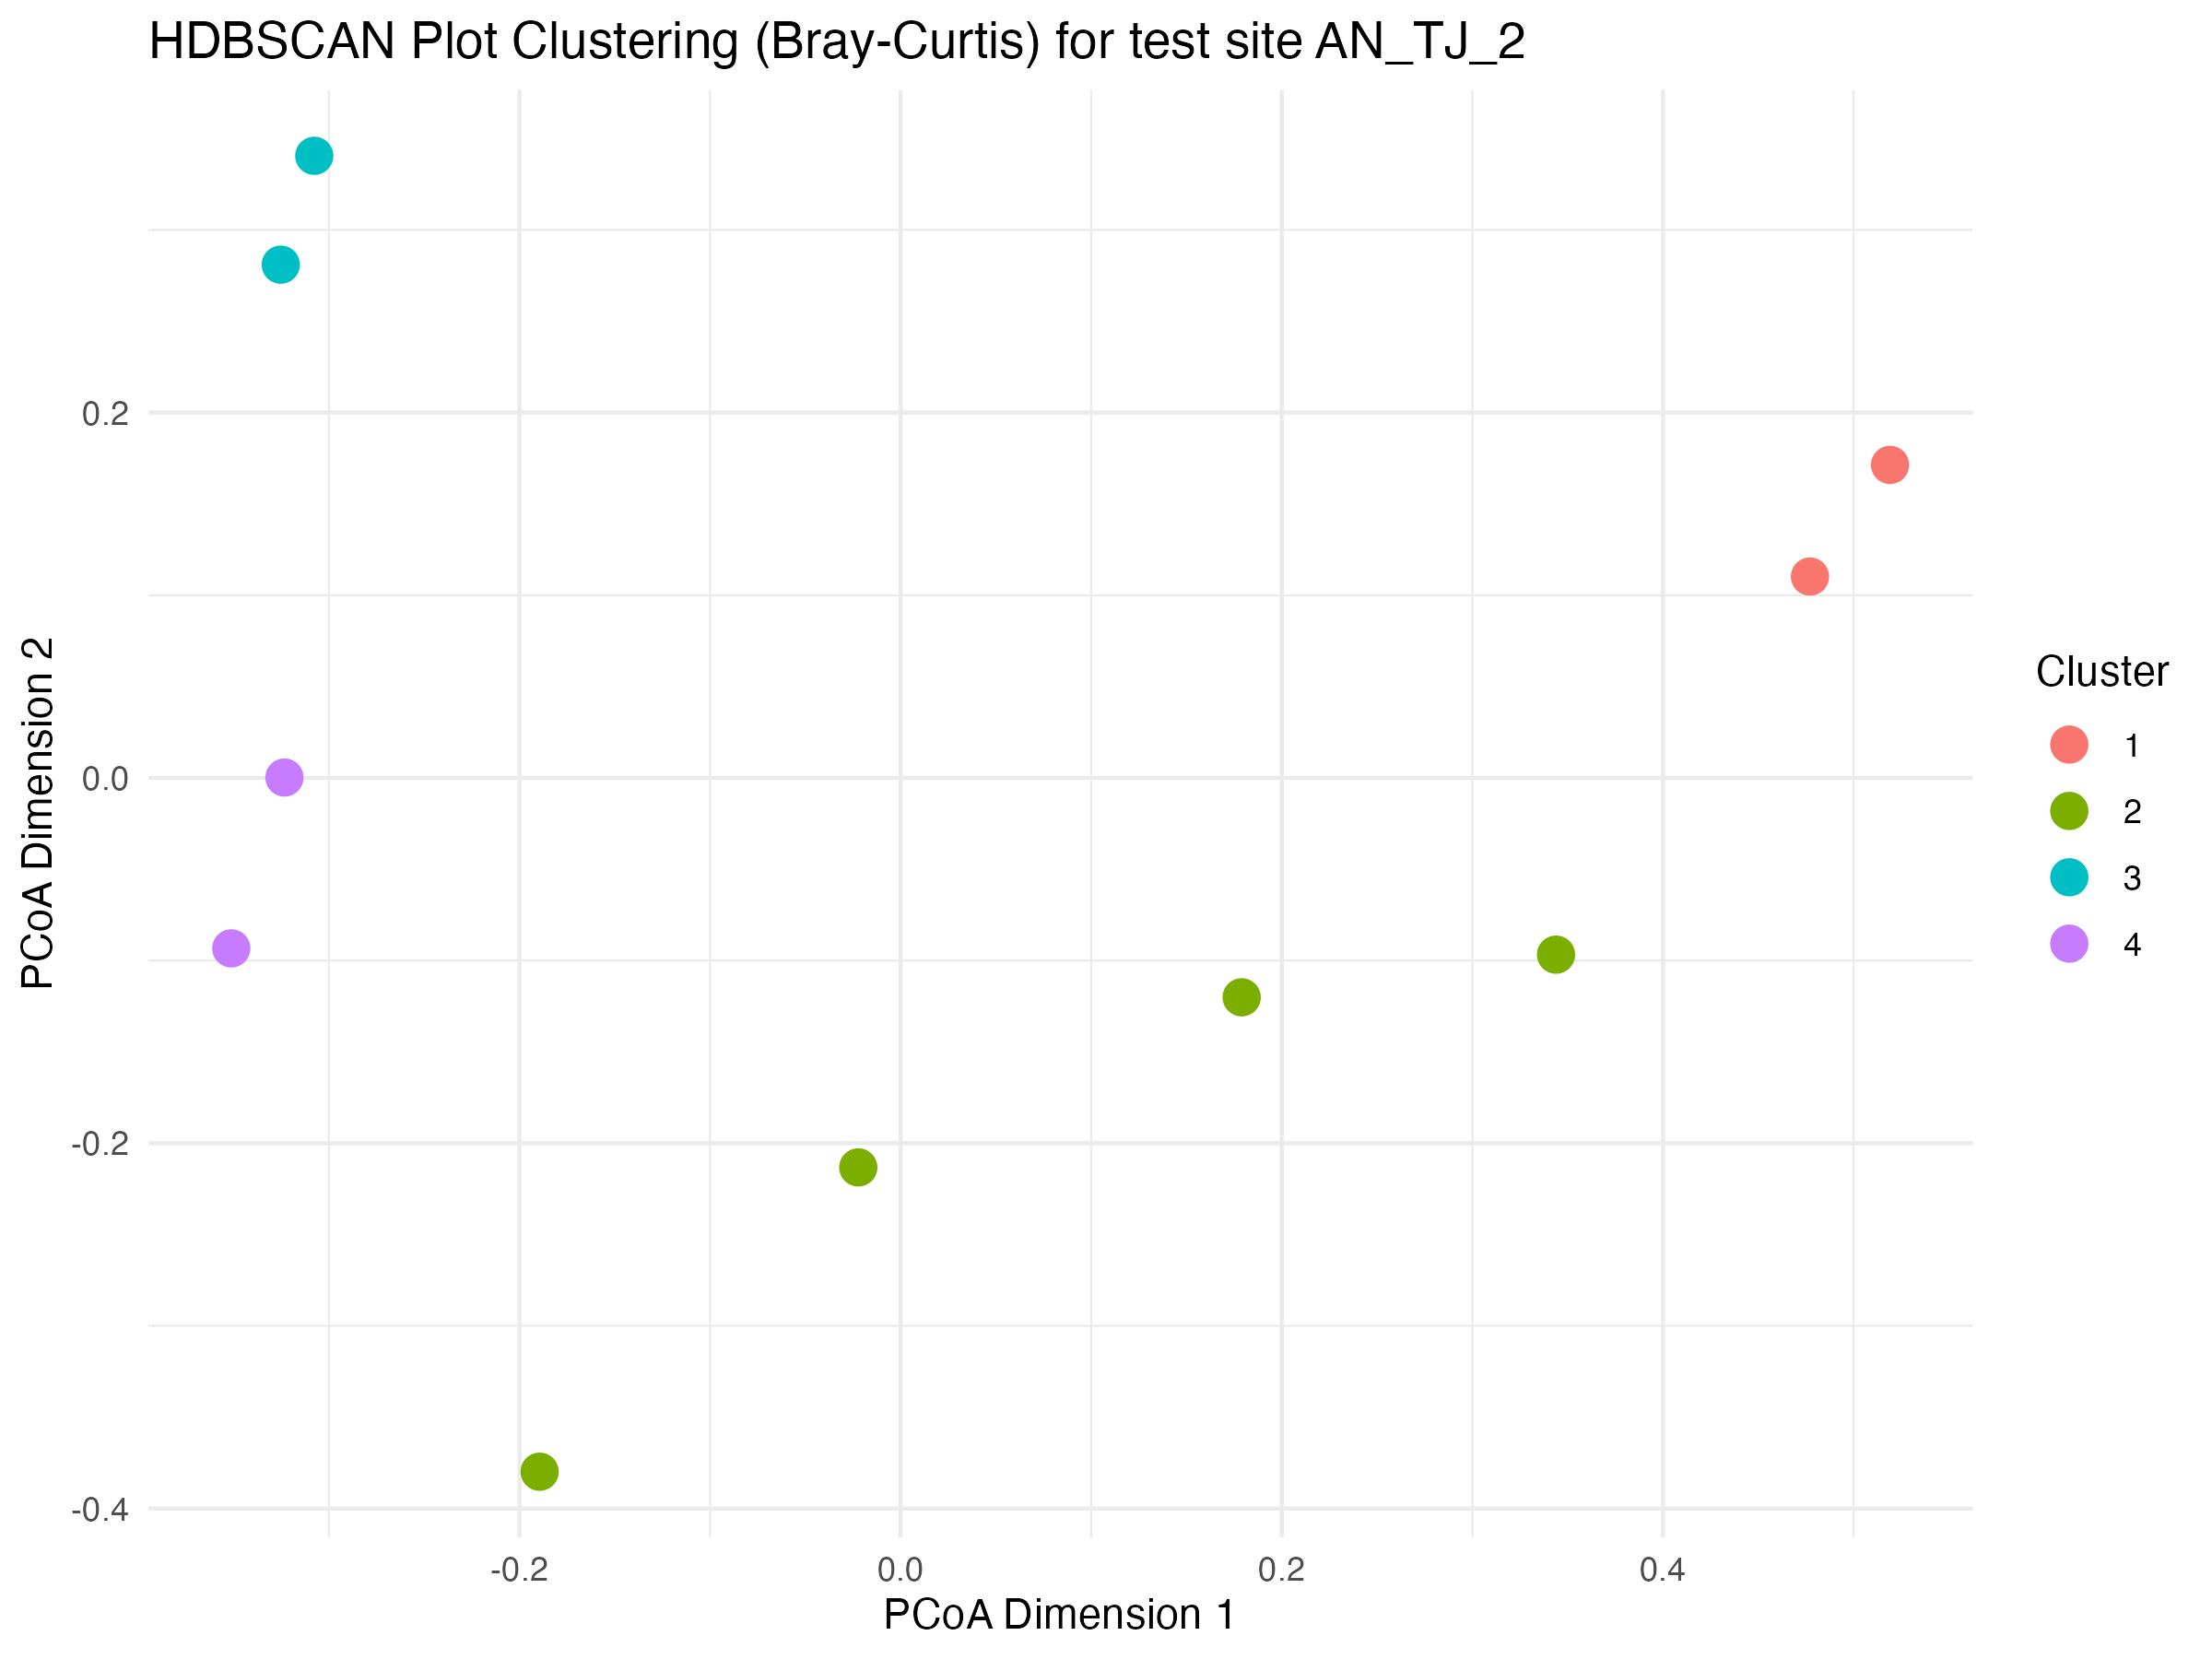
\includegraphics[width=\textwidth]{Figures/Appendix/PlantCommunityClustering/AN_TJ_2_HDBSCAN_clusters.png}
%         \caption{AN\_TJ\_2}
%         \label{fig:AN_TJ_2_HDBSCAN_clusters}
%     \end{minipage}

%     \vspace{1cm} % Space between rows of images

%     \begin{minipage}[b]{0.45\textwidth}
%         \centering
%         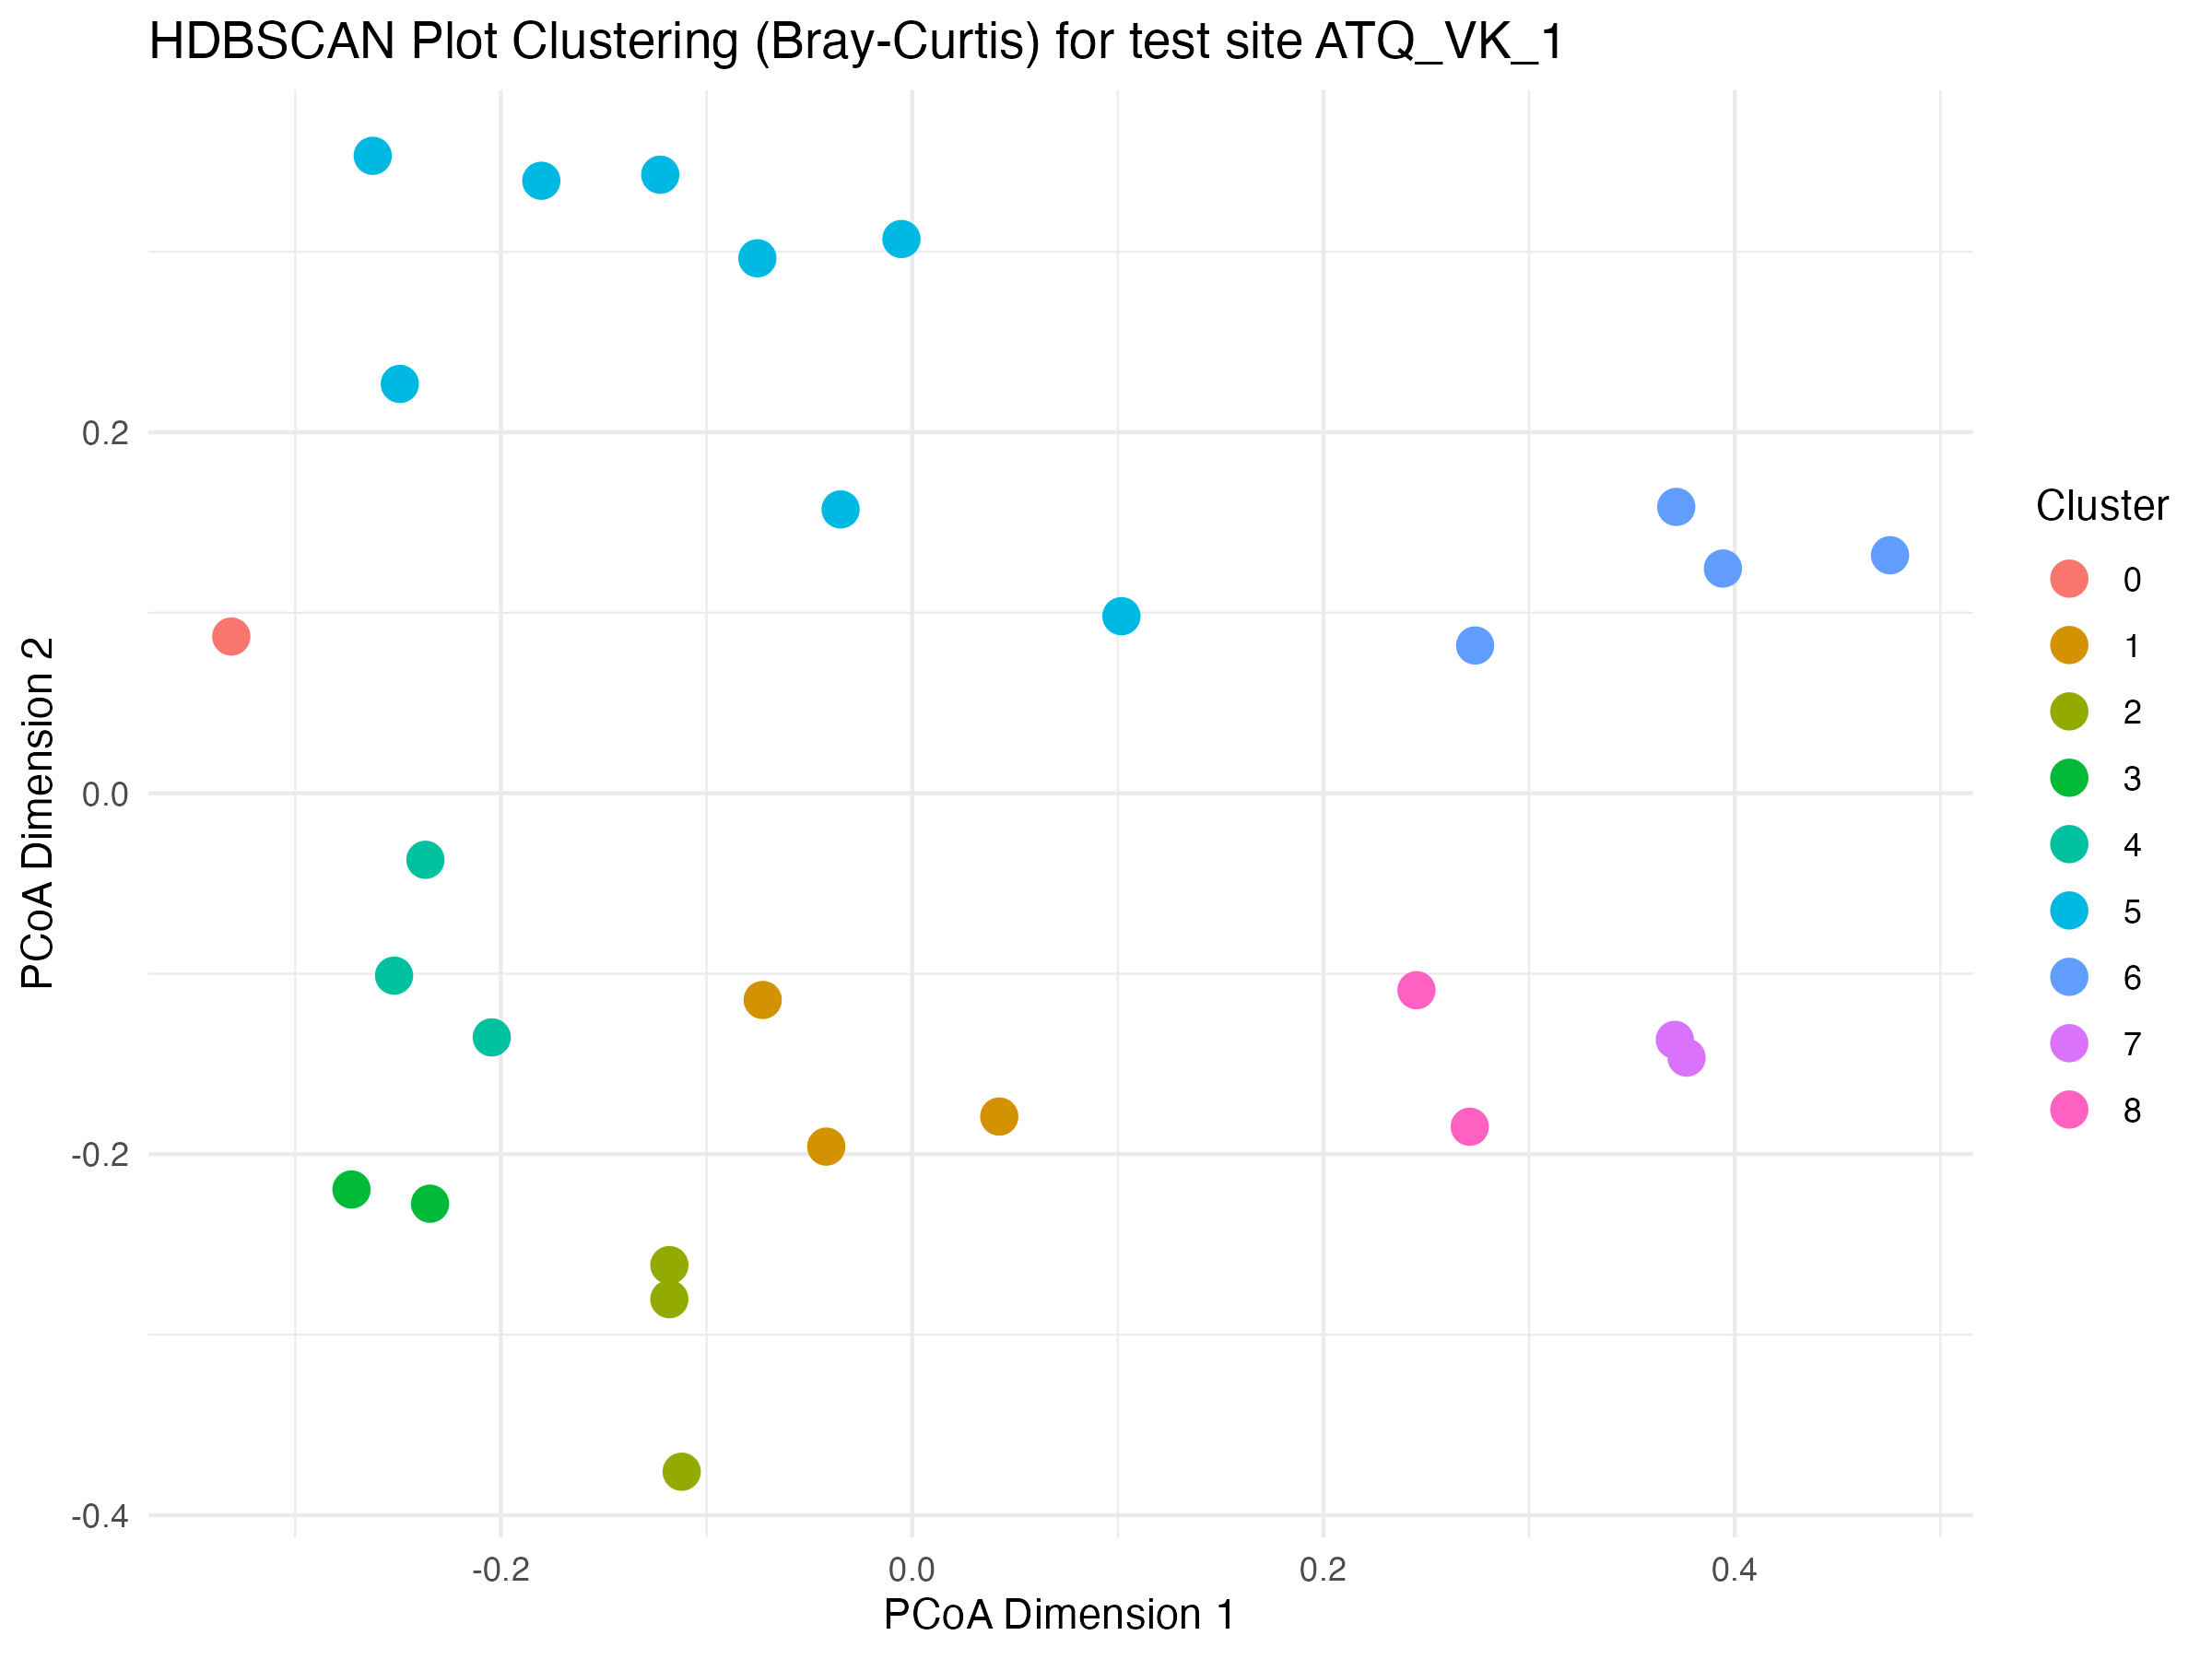
\includegraphics[width=\textwidth]{Figures/Appendix/PlantCommunityClustering/ATQ_VK_1_HDBSCAN_clusters.png}
%         \caption{ATQ\_VK\_1}
%         \label{fig:ATQ_VK_1_HDBSCAN_clusters}
%     \end{minipage}
%     \hfill
%     \begin{minipage}[b]{0.45\textwidth}
%         \centering
%         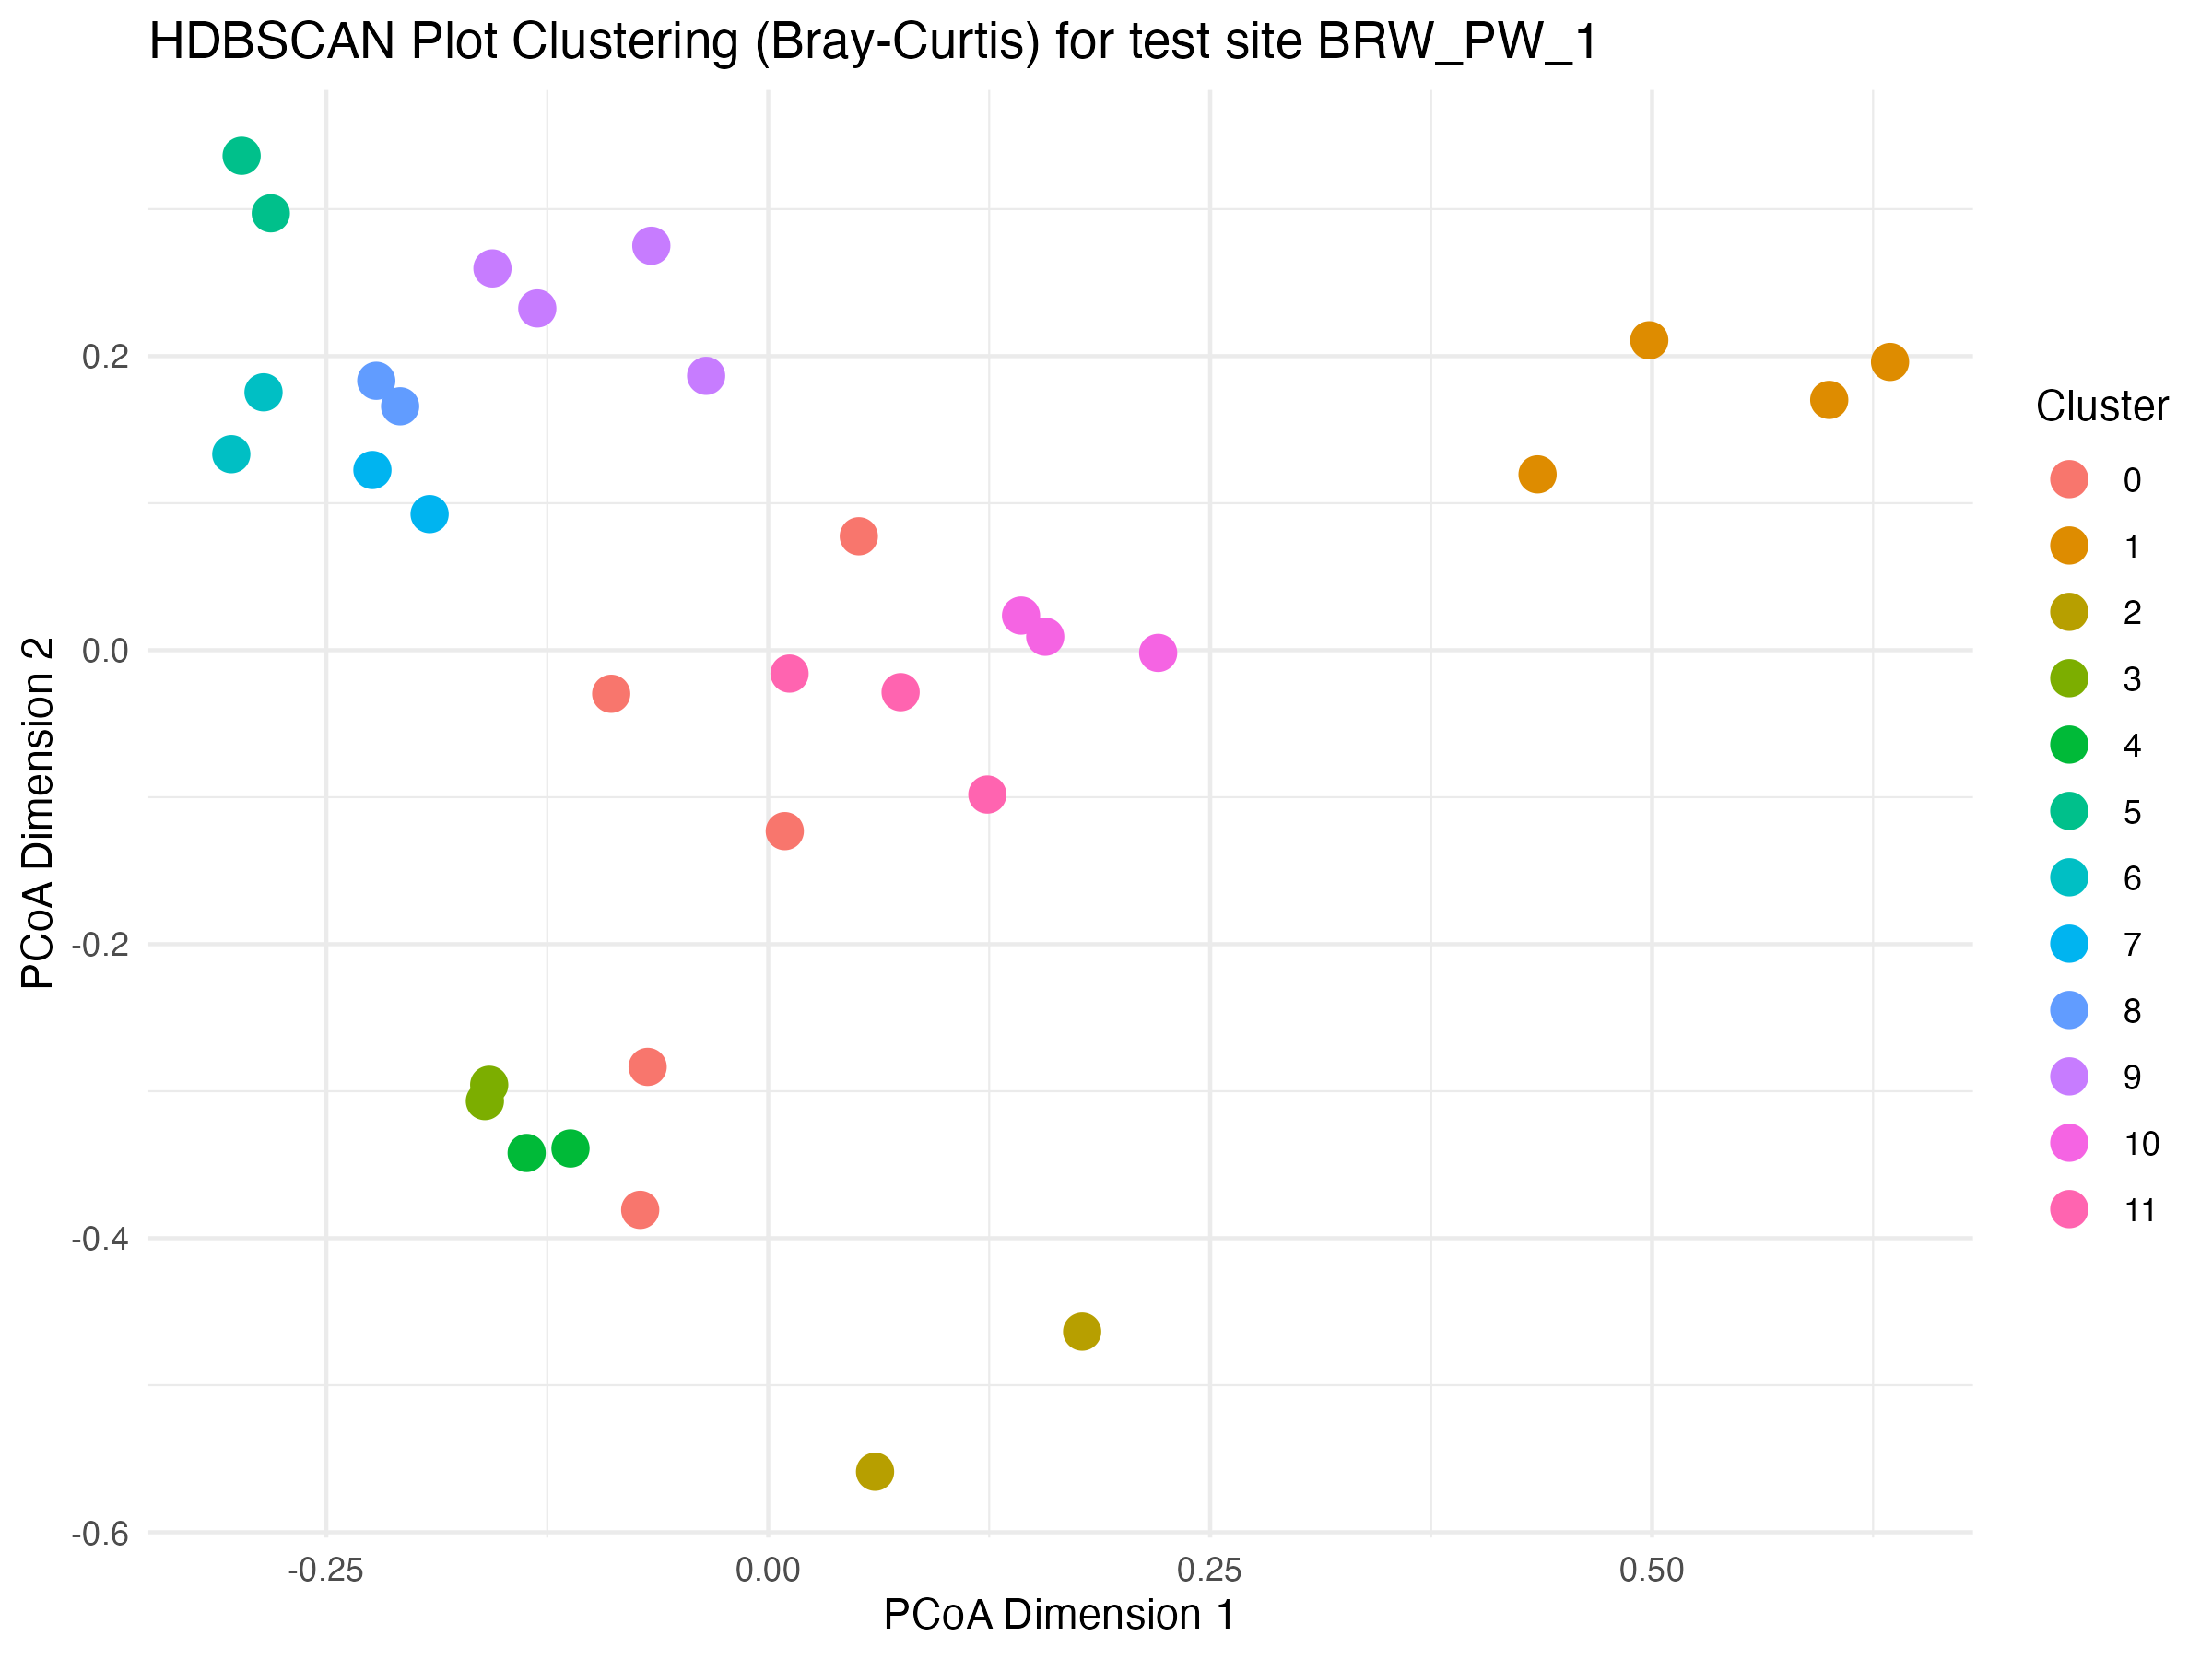
\includegraphics[width=\textwidth]{Figures/Appendix/PlantCommunityClustering/BRW_PW_1_HDBSCAN_clusters.png}
%         \caption{BRW\_PW\_1}
%         \label{fig:BRW_PW_1_HDBSCAN_clusters}
%     \end{minipage}
%     \captionof{figure}{Community Cluster Plots for Test Sites AN\_TJ\_1, AN\_TJ\_2, ATQ\_VK\_1, and BRW\_PW\_1}
%     \label{fig:group1_clusters}
% \end{figure}

% % Group 2 of 4
% \begin{figure}[H]
%     \centering
%     \begin{minipage}[b]{0.45\textwidth}
%         \centering
%         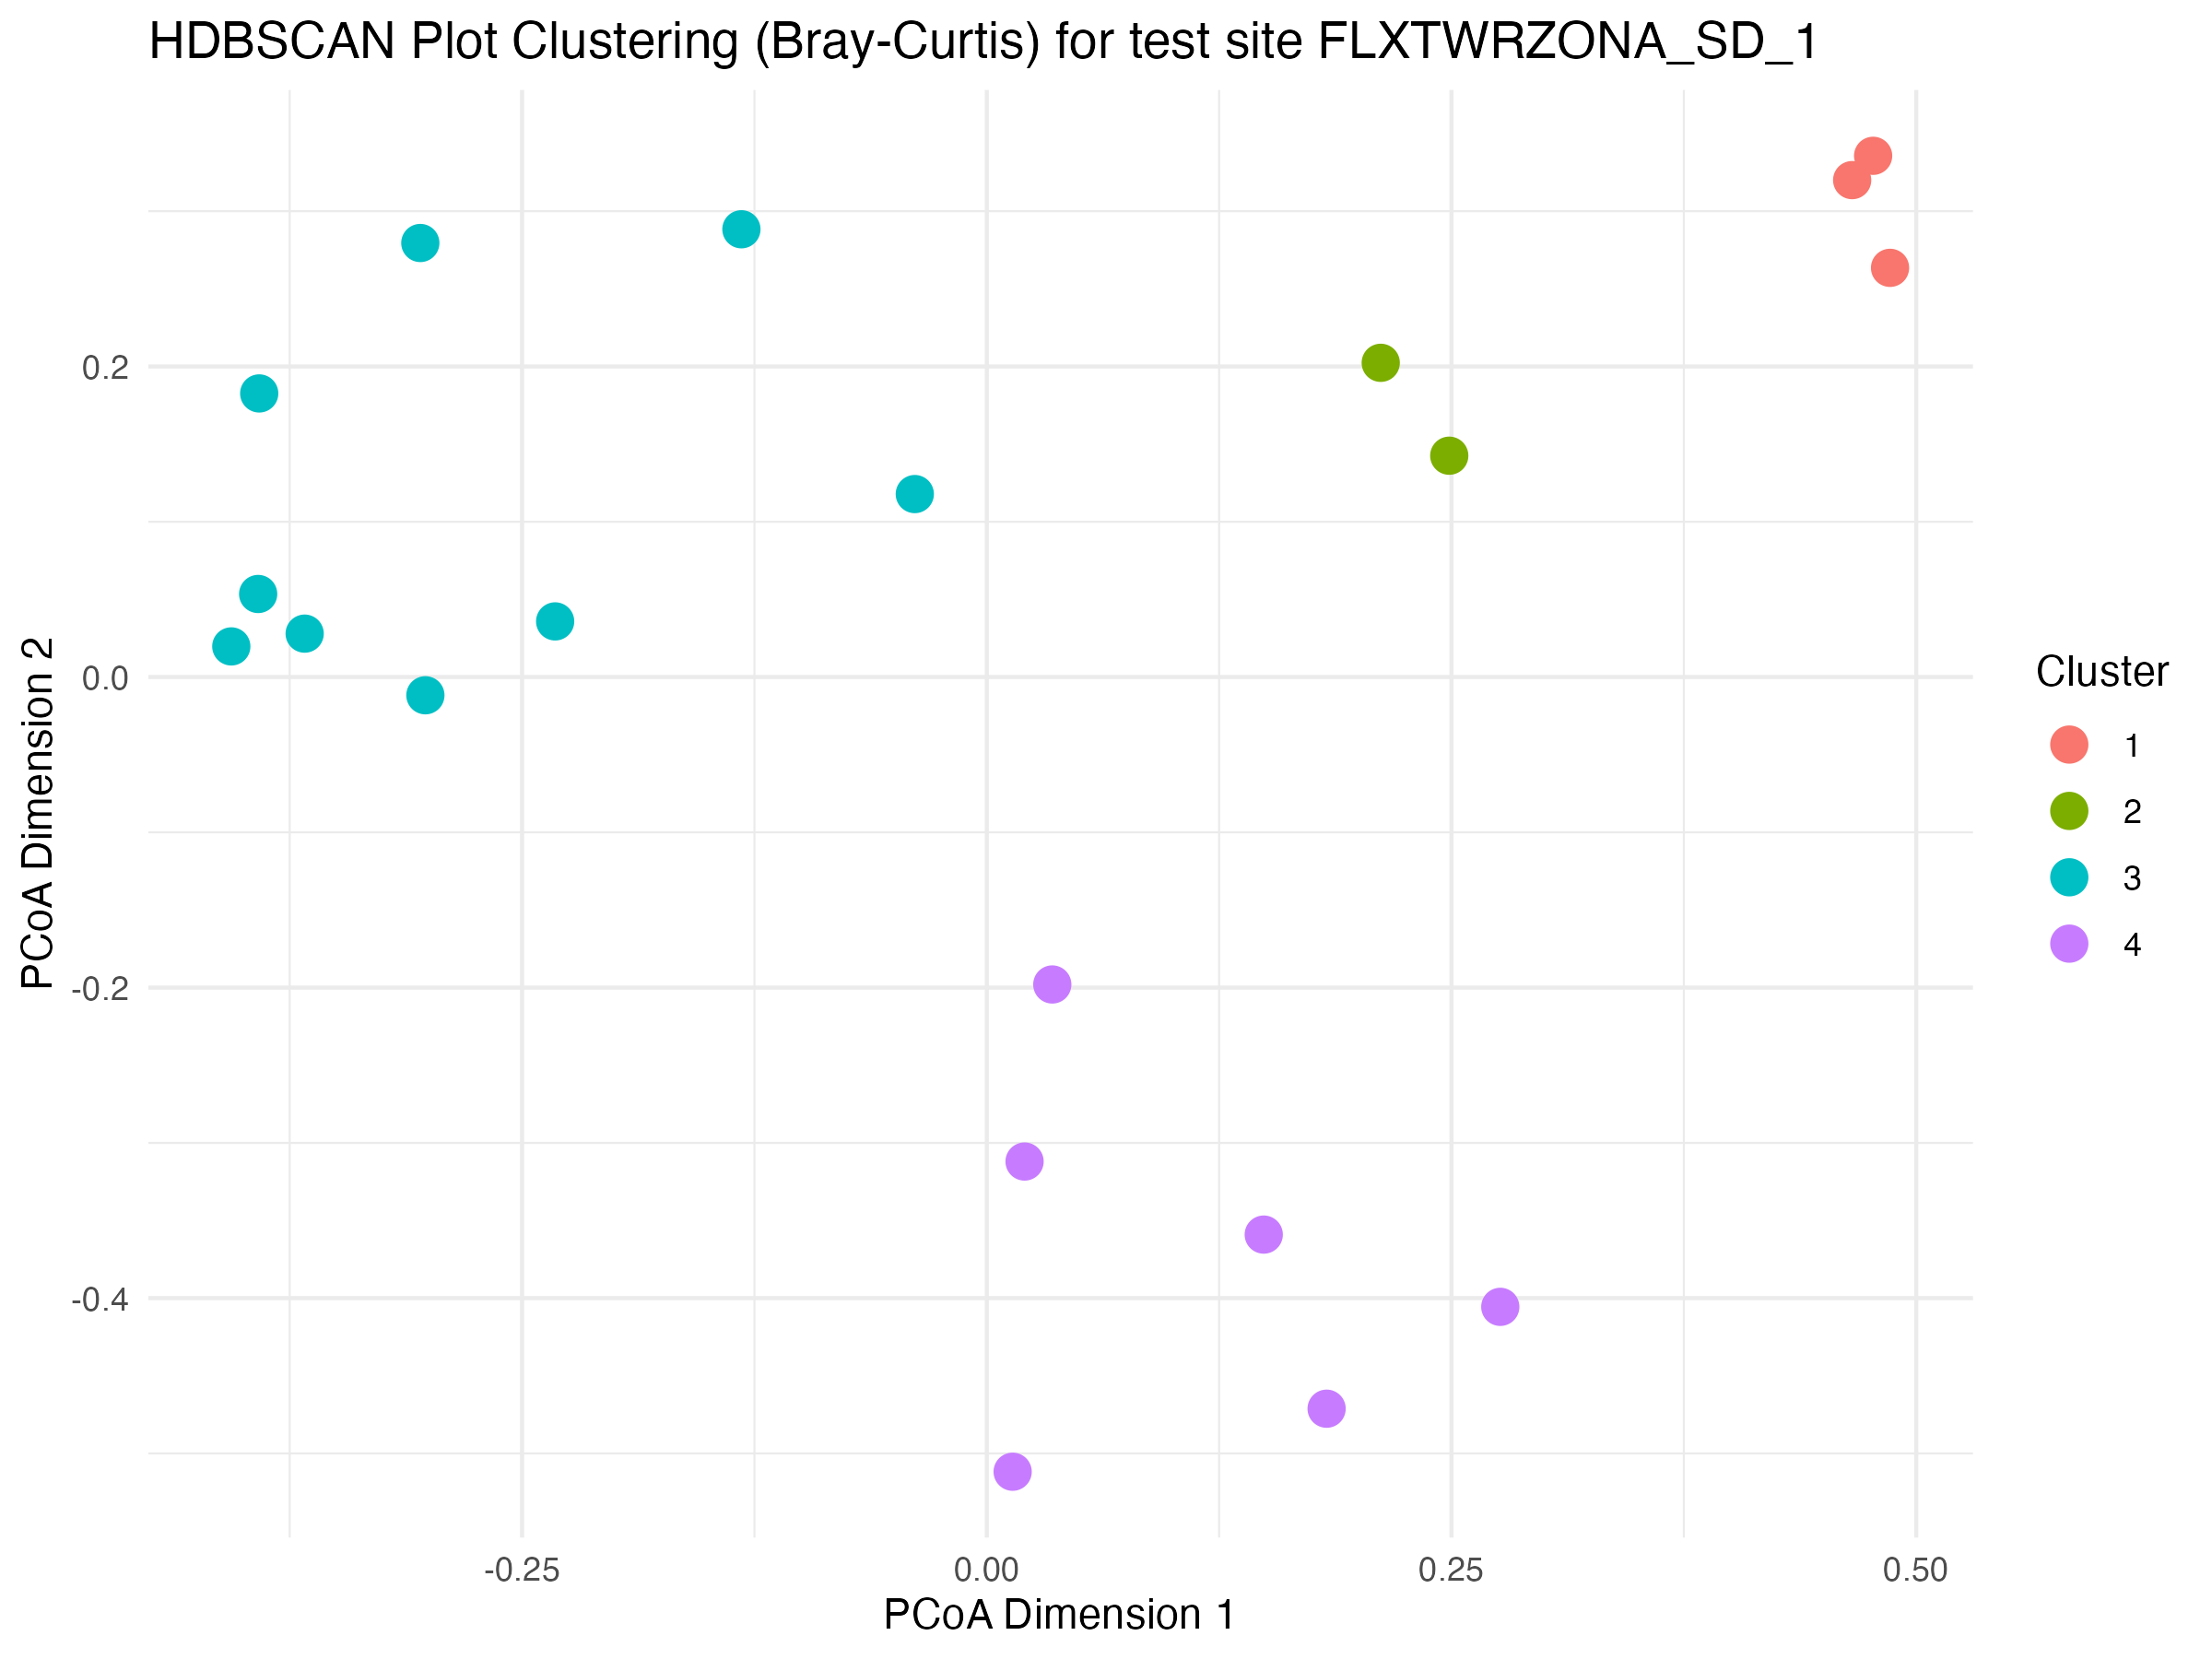
\includegraphics[width=\textwidth]{Figures/Appendix/PlantCommunityClustering/FLXTWRZONA_SD_1_HDBSCAN_clusters.png}
%         \caption{FLXTWRZONA\_SD\_1}
%         \label{fig:FLXTWRZONA_SD_1_HDBSCAN_clusters}
%     \end{minipage}
%     \hfill
%     \begin{minipage}[b]{0.45\textwidth}
%         \centering
%         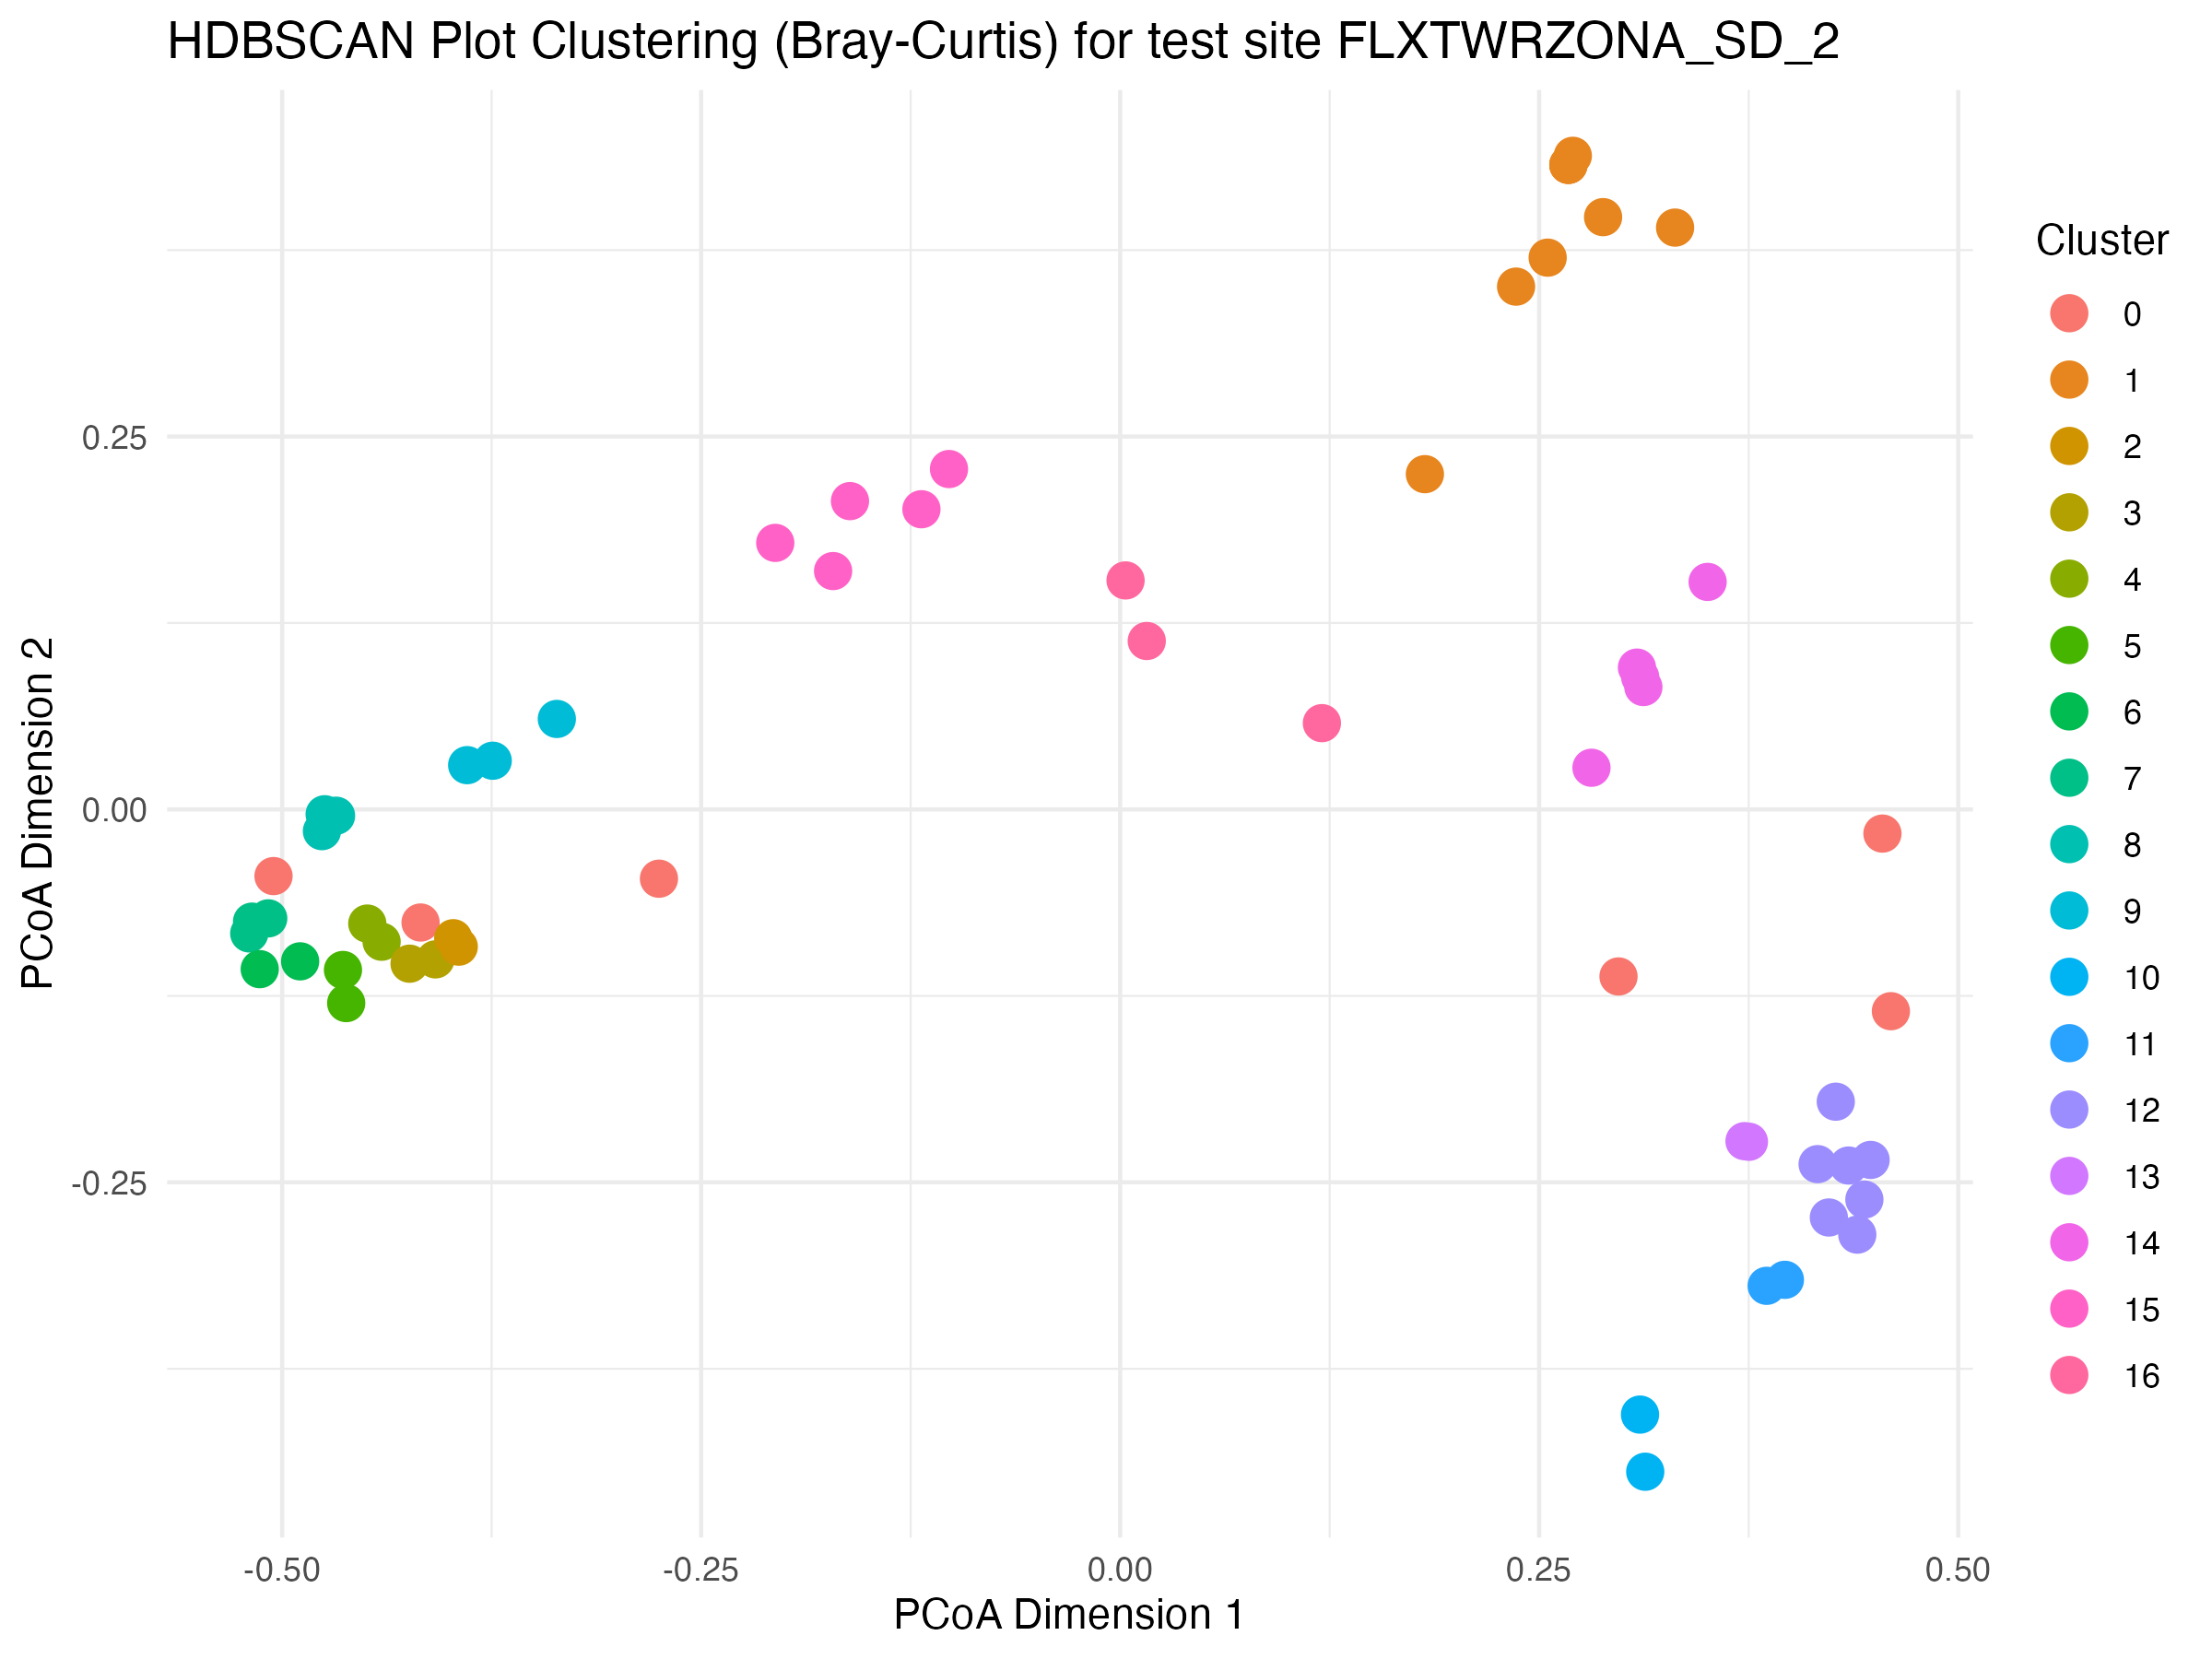
\includegraphics[width=\textwidth]{Figures/Appendix/PlantCommunityClustering/FLXTWRZONA_SD_2_HDBSCAN_clusters.png}
%         \caption{FLXTWRZONA\_SD\_2}
%         \label{fig:FLXTWRZONA_SD_2_HDBSCAN_clusters}
%     \end{minipage}

%     \vspace{1cm} % Space between rows of images

%     \begin{minipage}[b]{0.45\textwidth}
%         \centering
%         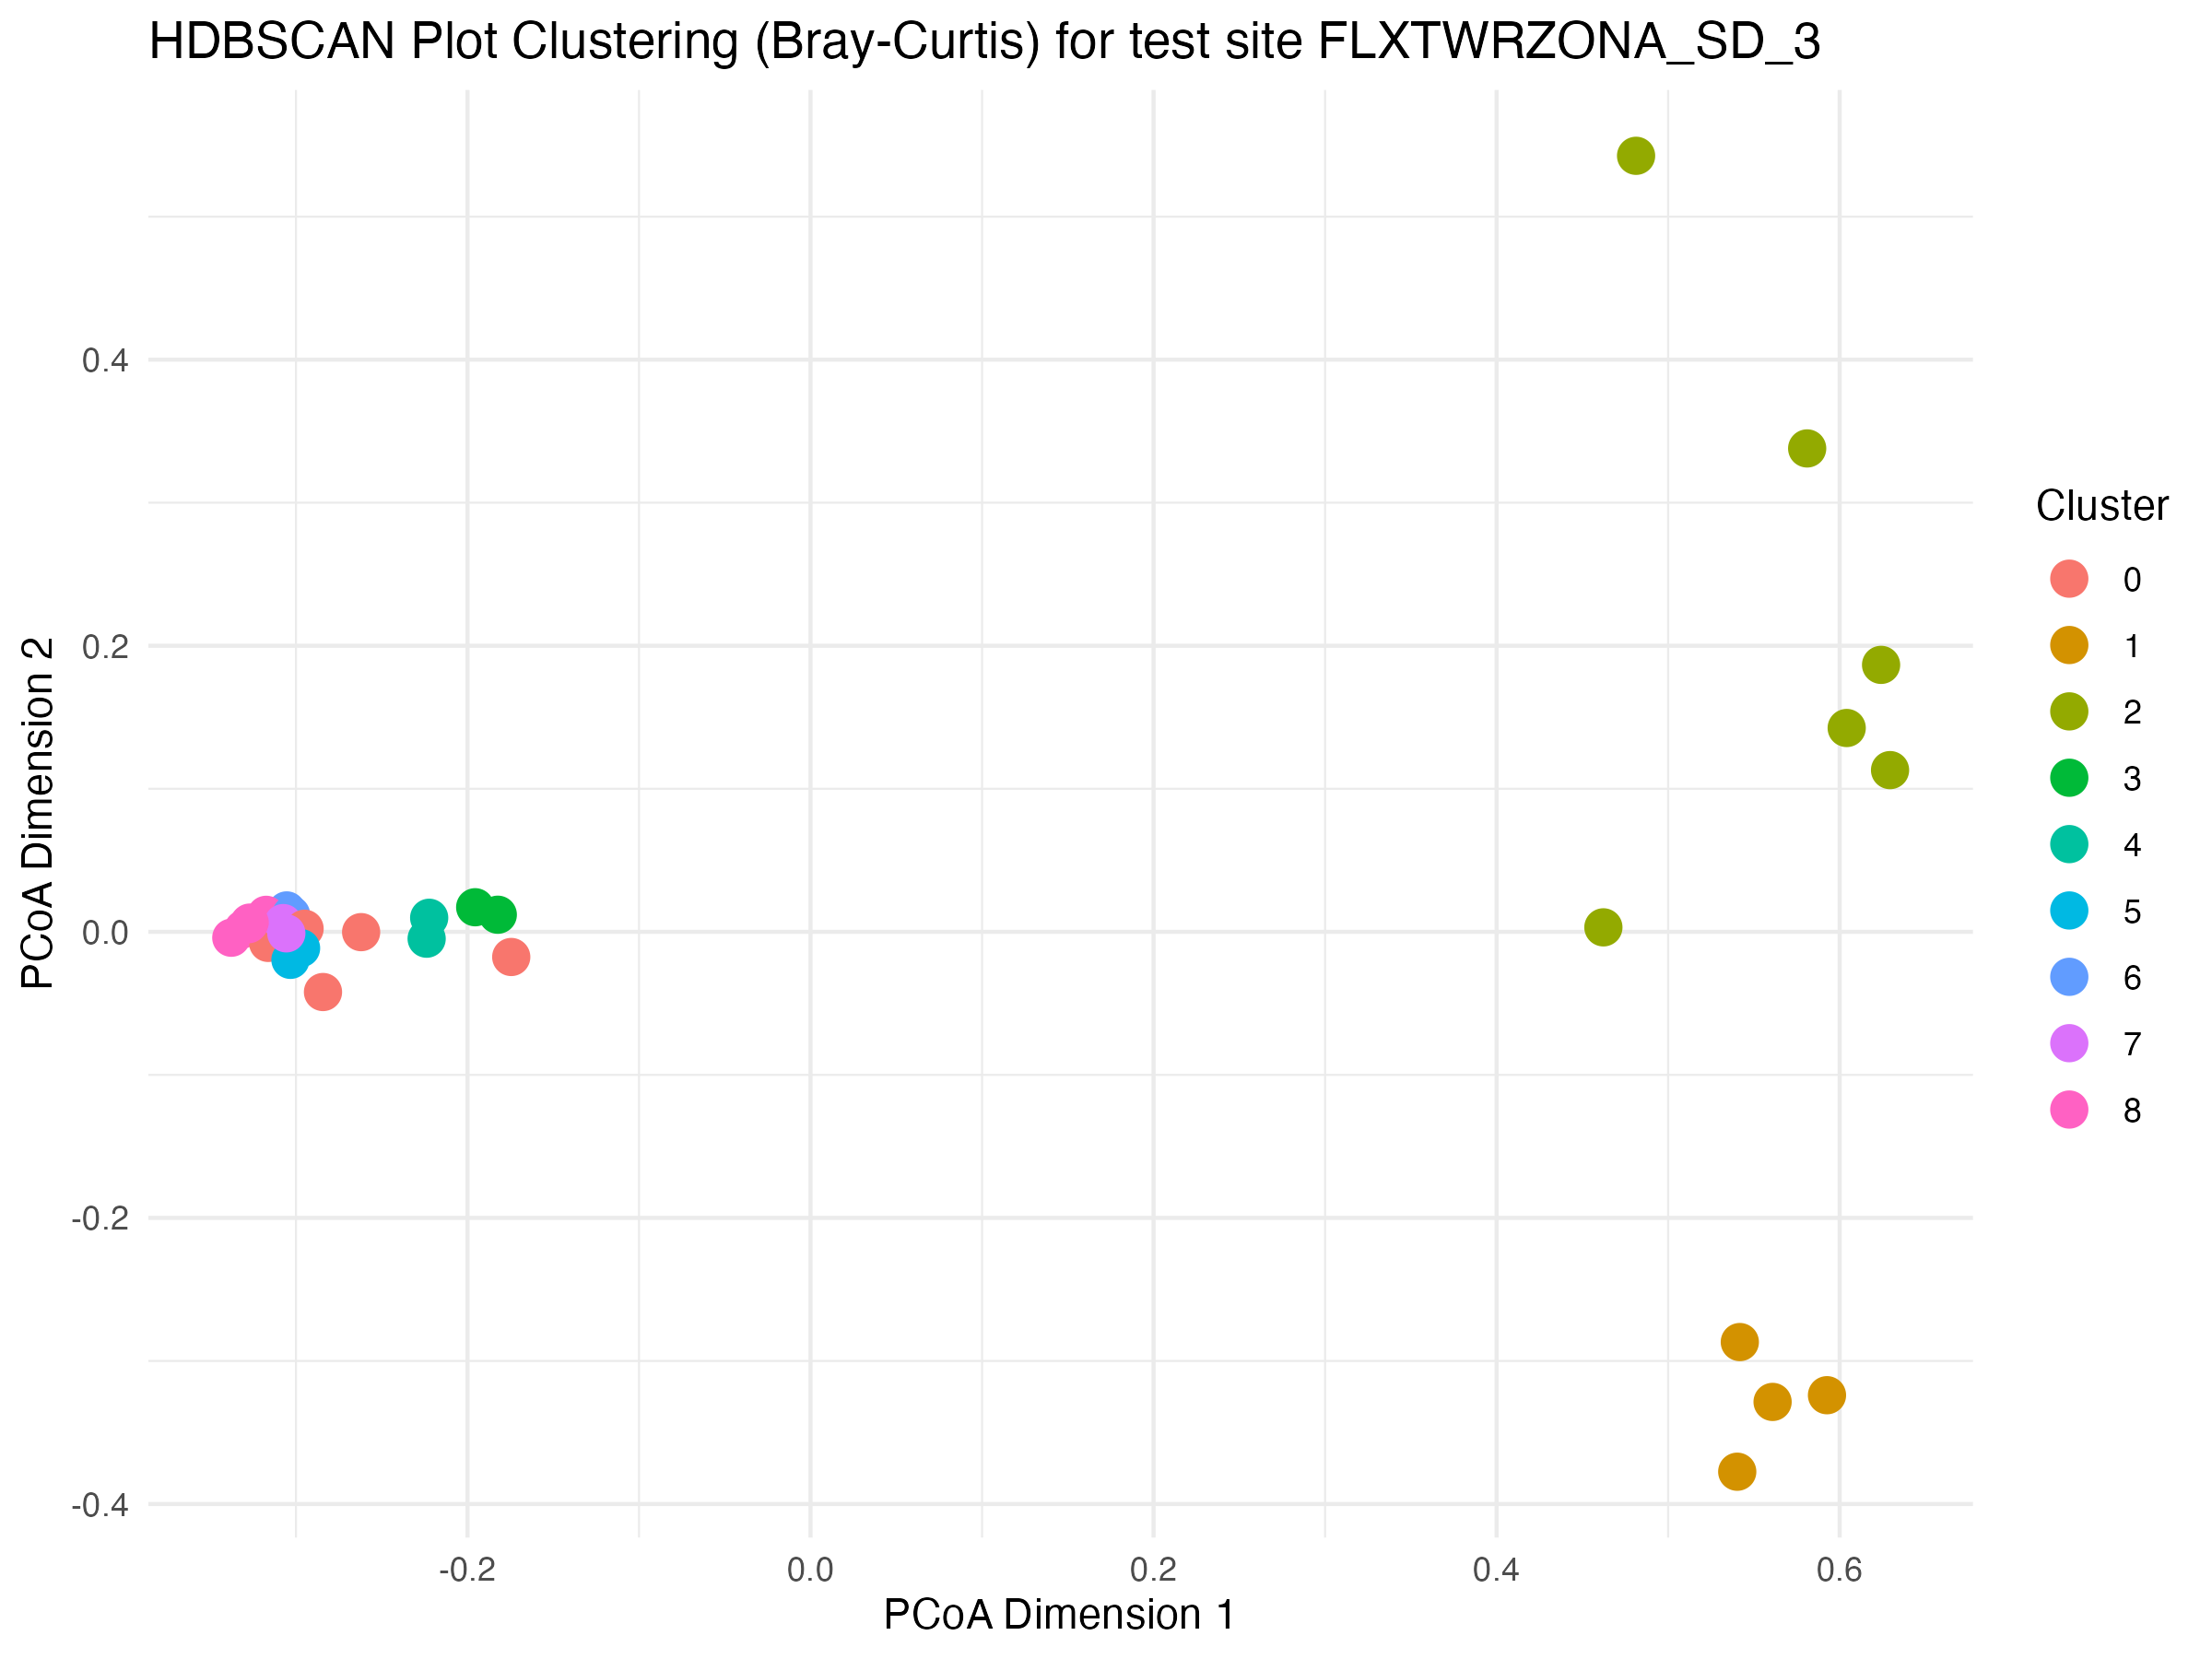
\includegraphics[width=\textwidth]{Figures/Appendix/PlantCommunityClustering/FLXTWRZONA_SD_3_HDBSCAN_clusters.png}
%         \caption{FLXTWRZONA\_SD\_3}
%         \label{fig:FLXTWRZONA_SD_3_HDBSCAN_clusters}
%     \end{minipage}
%     \hfill
%     \begin{minipage}[b]{0.45\textwidth}
%         \centering
%         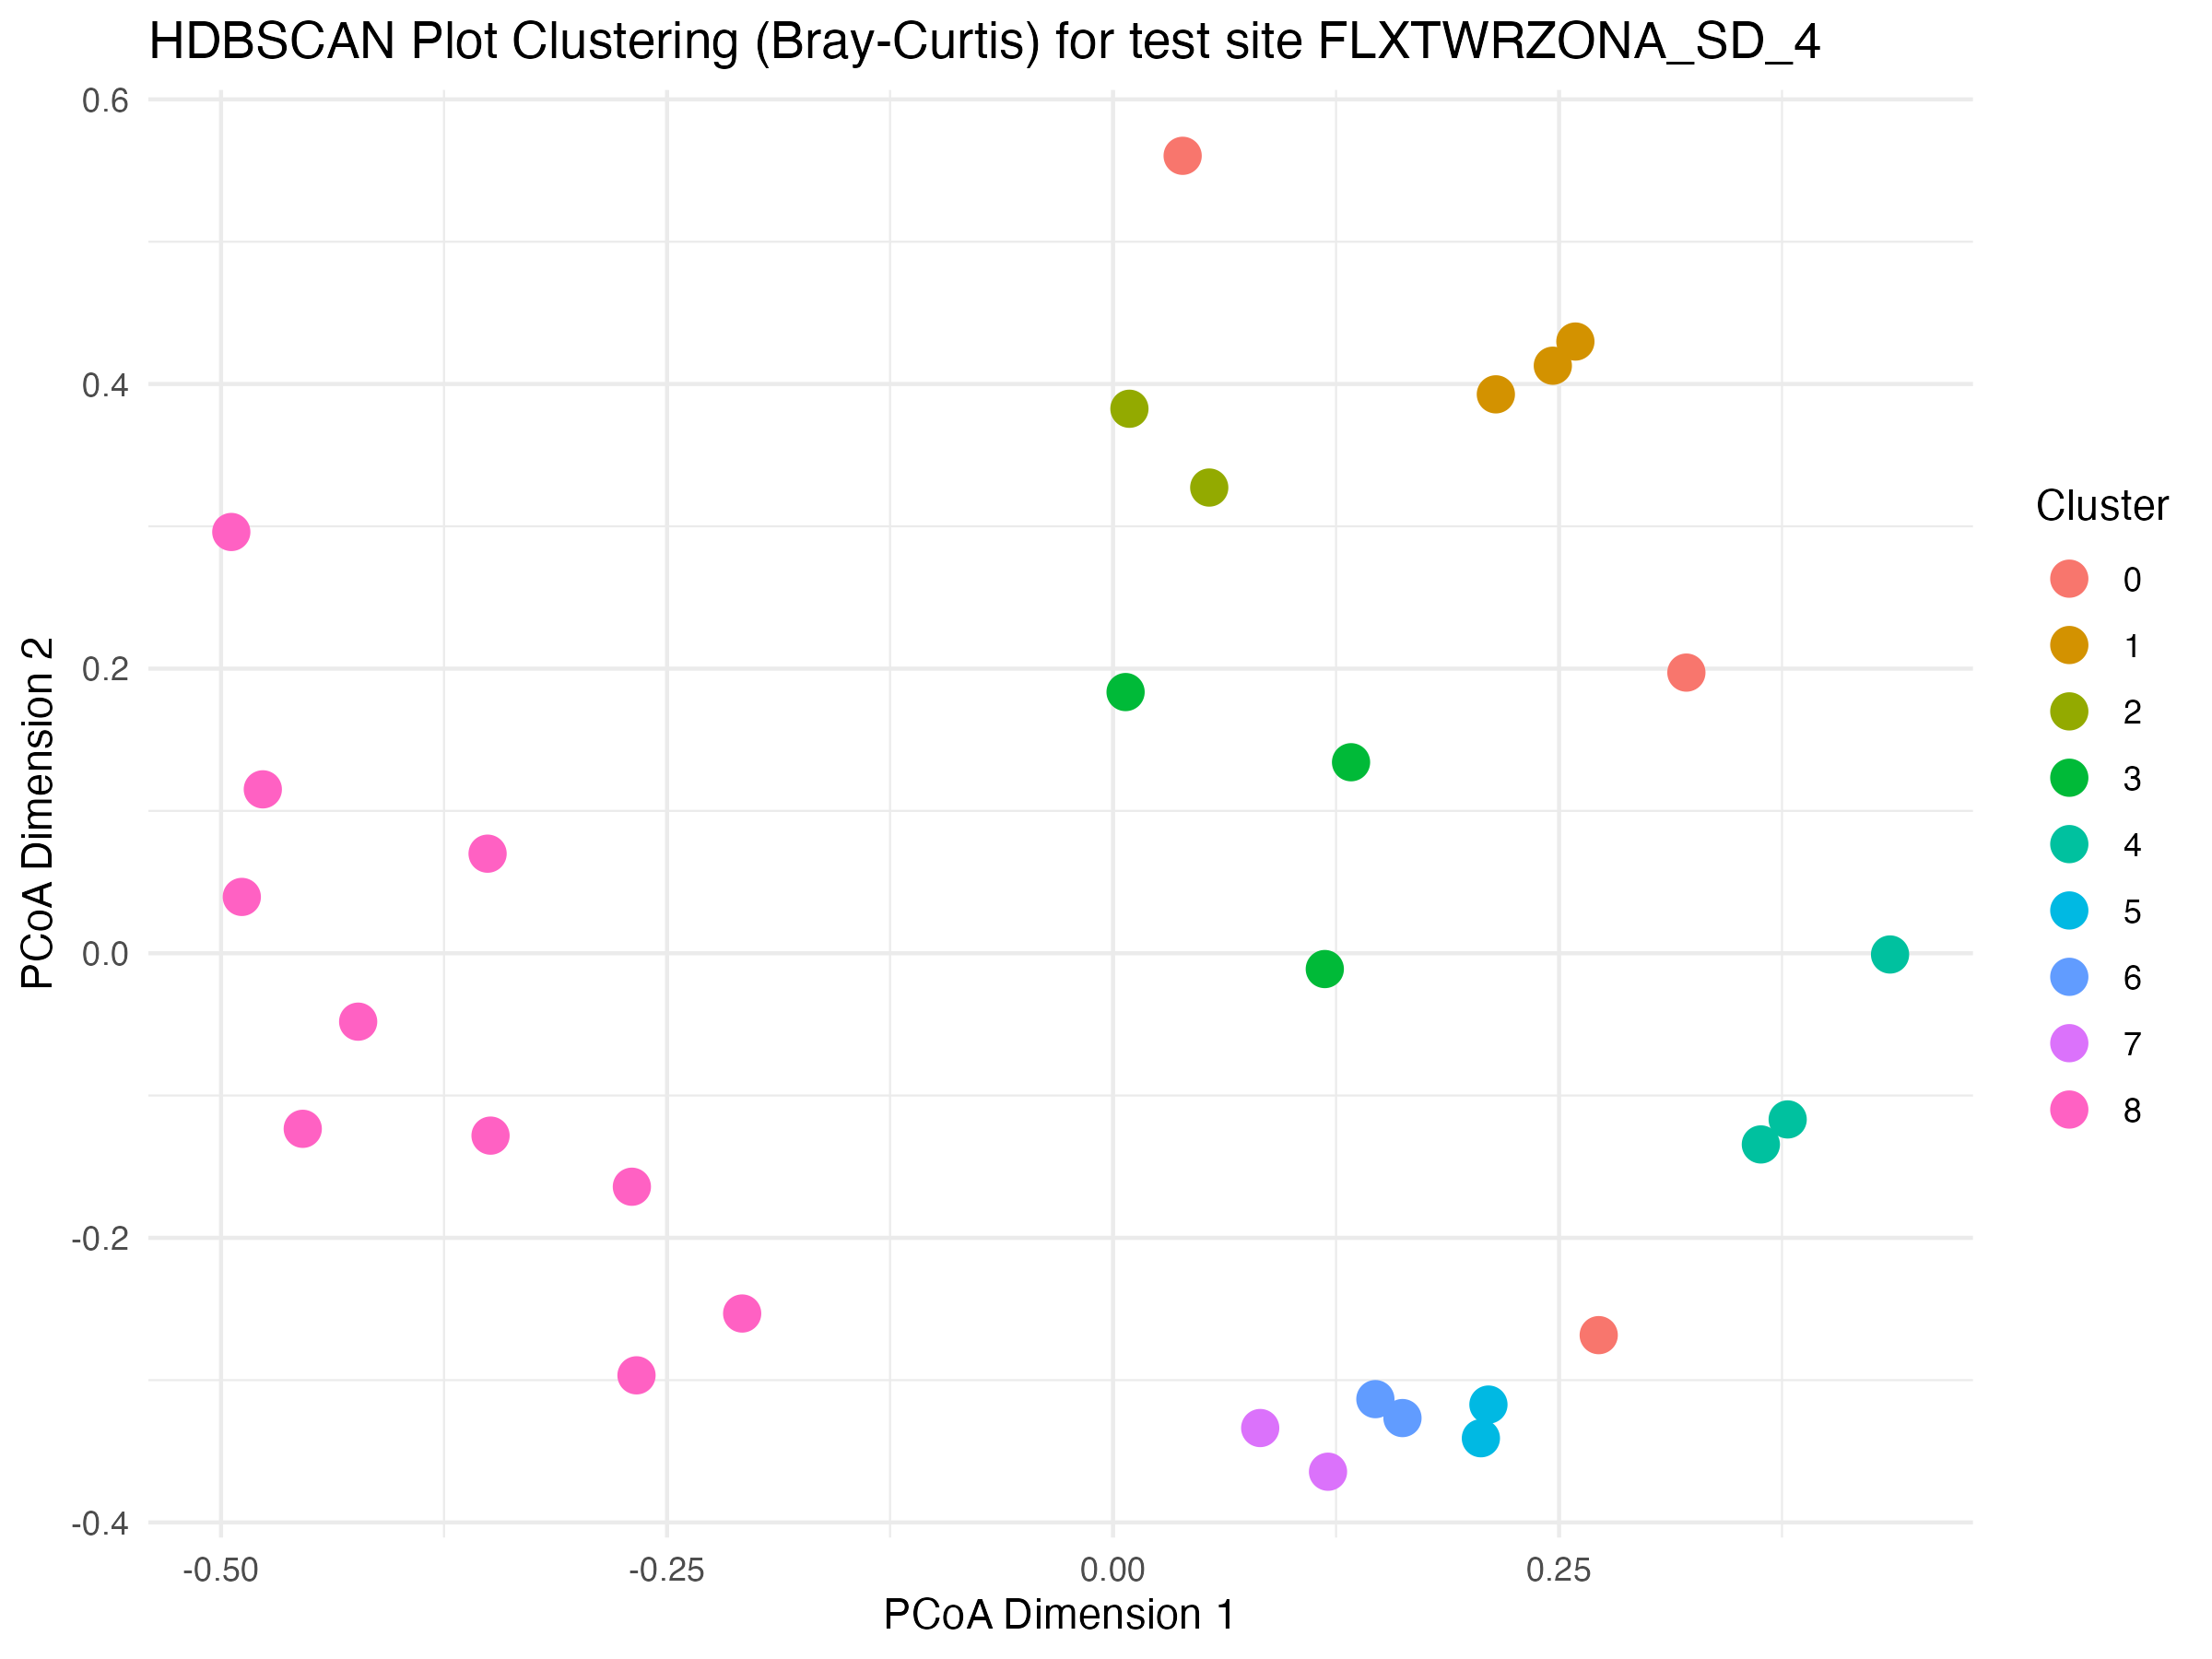
\includegraphics[width=\textwidth]{Figures/Appendix/PlantCommunityClustering/FLXTWRZONA_SD_4_HDBSCAN_clusters.png}
%         \caption{FLXTWRZONA\_SD\_4}
%         \label{fig:FLXTWRZONA_SD_4_HDBSCAN_clusters}
%     \end{minipage}
%     \captionof{figure}{Community Cluster Plots for Test Sites FLXTWRZONA\_SD\_1, FLXTWRZONA\_SD\_2, FLXTWRZONA\_SD\_3, and FLXTWRZONA\_SD\_4}
%     \label{fig:group2_clusters}
% \end{figure}

% % Group 3 of 4 (remaining plots)
% \begin{figure}[H]
%     \centering
%     \begin{minipage}[b]{0.45\textwidth}
%         \centering
%         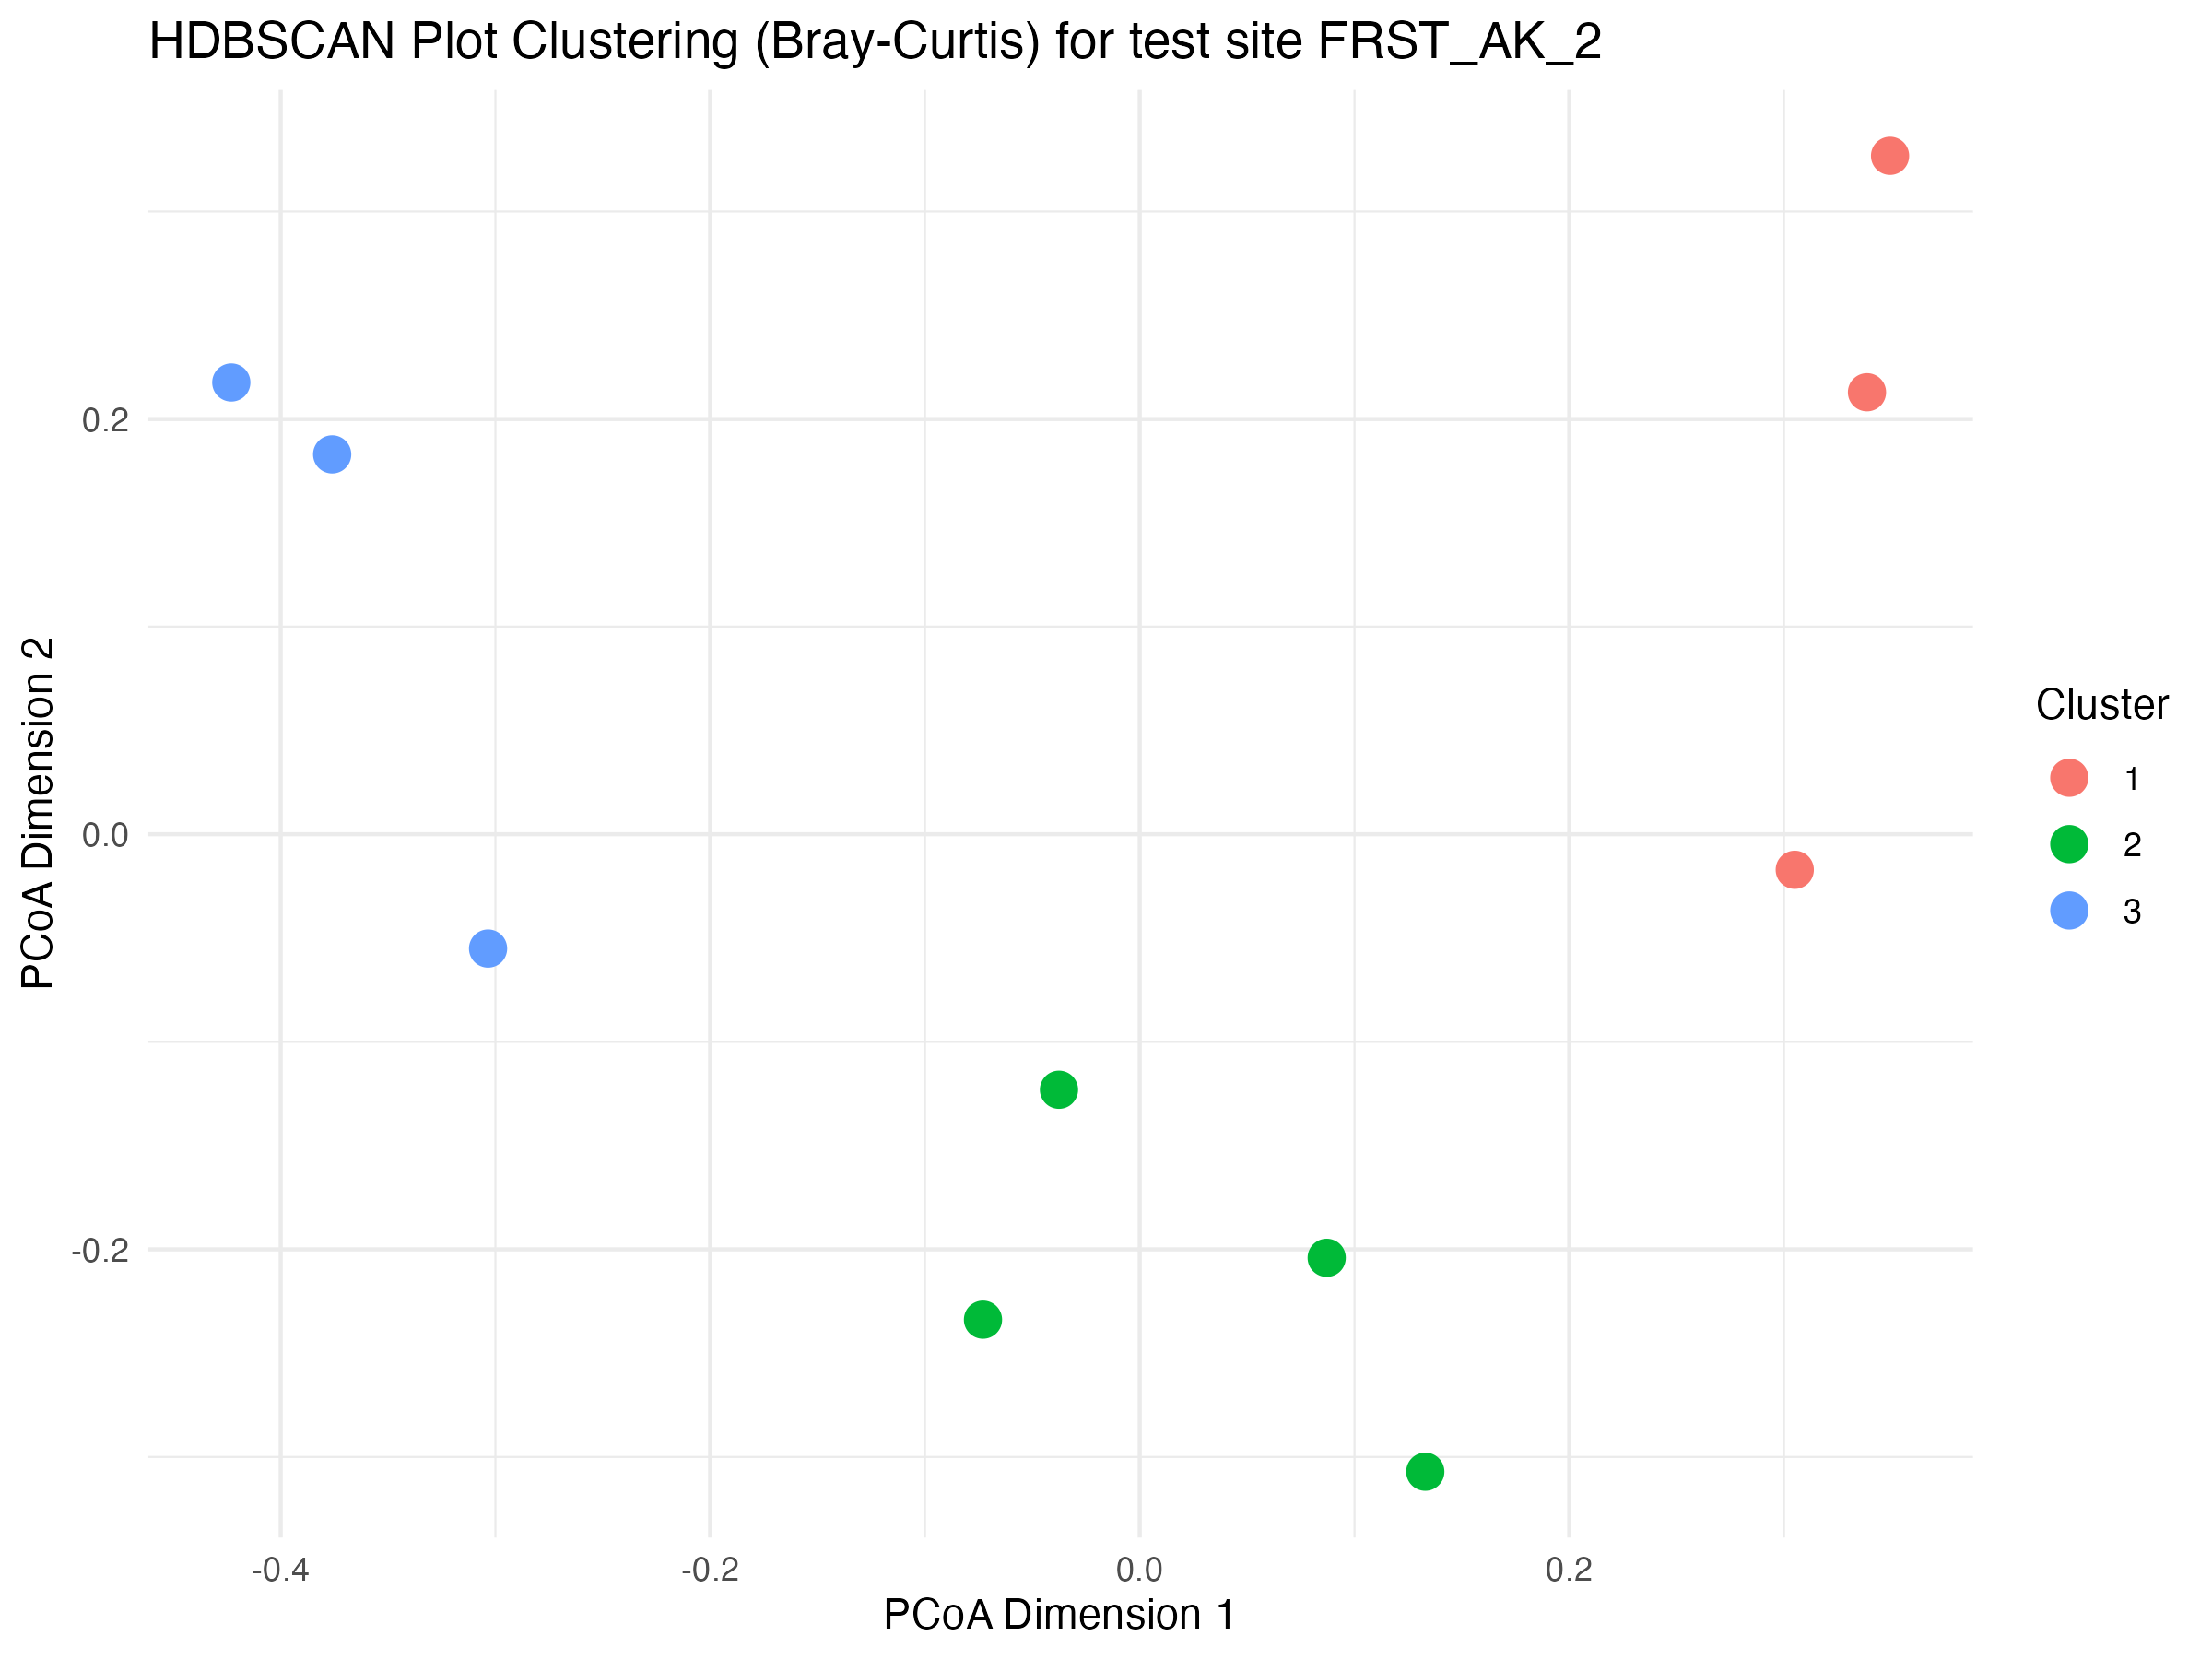
\includegraphics[width=\textwidth]{Figures/Appendix/PlantCommunityClustering/FRST_AK_2_HDBSCAN_clusters.png}
%         \caption{FRST\_AK\_2}
%         \label{fig:FRST_AK_2_HDBSCAN_clusters}
%     \end{minipage}
%     \hfill
%     \begin{minipage}[b]{0.45\textwidth}
%         \centering
%         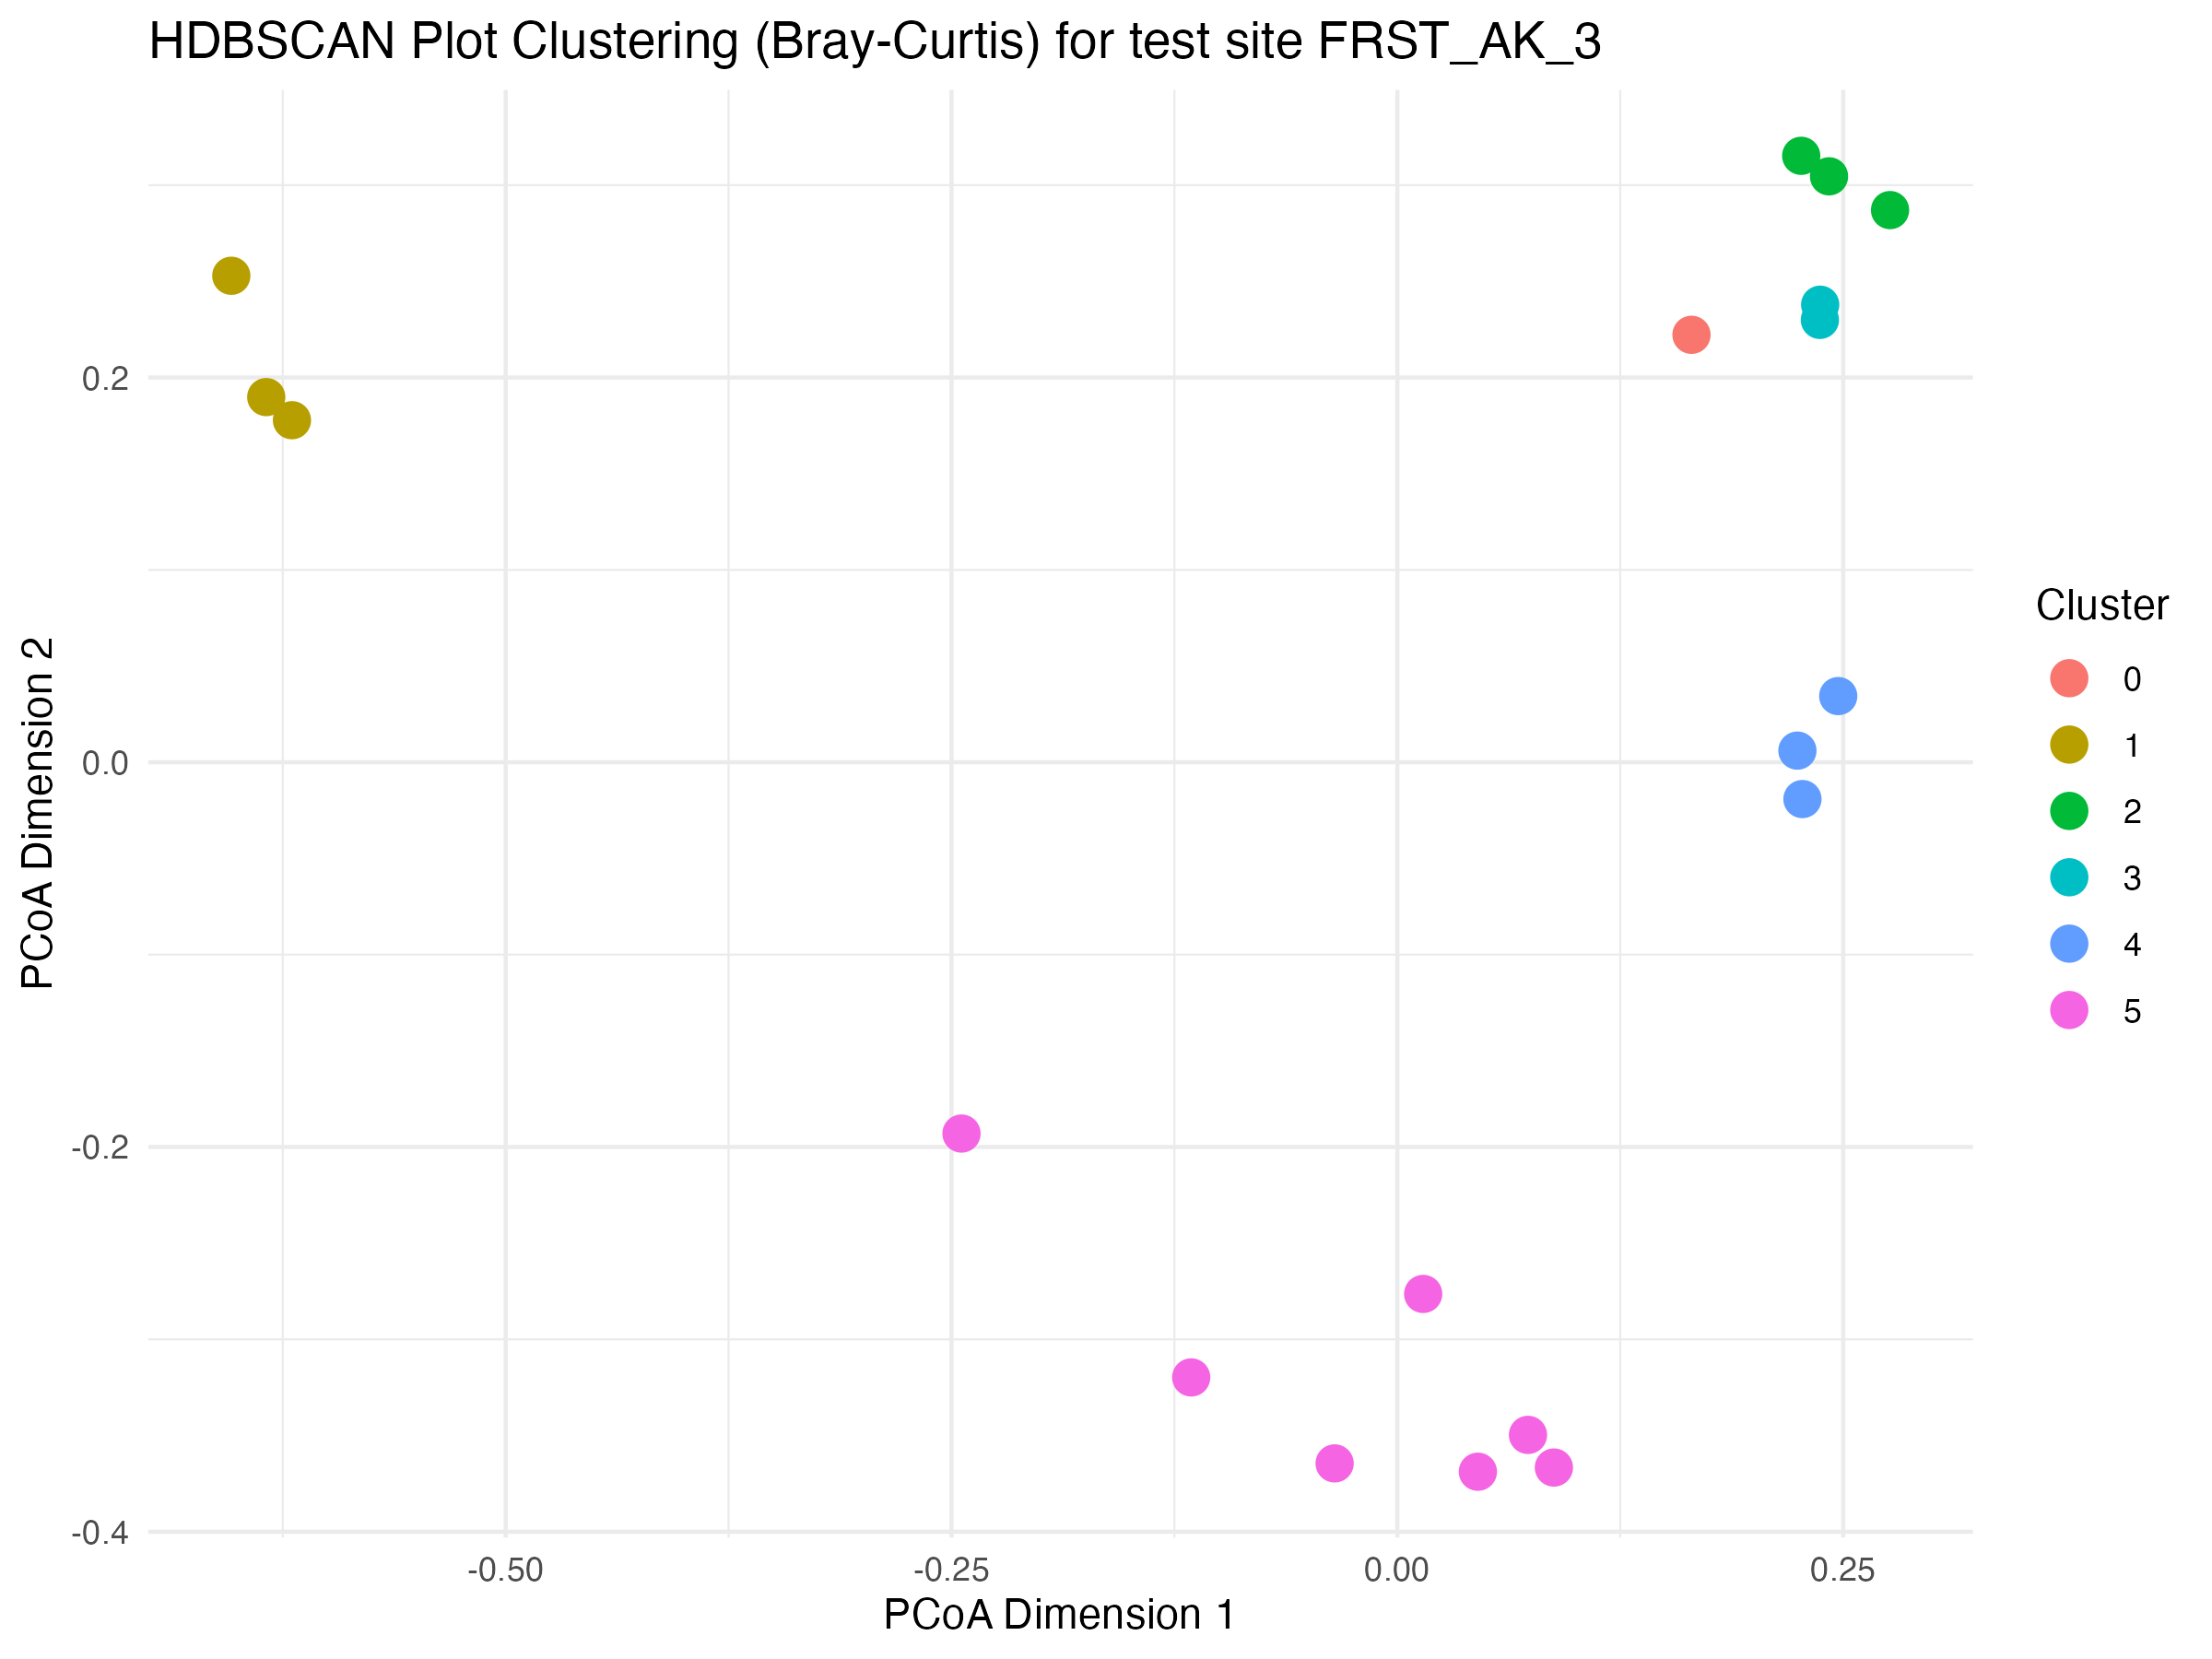
\includegraphics[width=\textwidth]{Figures/Appendix/PlantCommunityClustering/FRST_AK_3_HDBSCAN_clusters.png}
%         \caption{FRST\_AK\_3}
%         \label{fig:FRST_AK_3_HDBSCAN_clusters}
%     \end{minipage}

%     \vspace{1cm} % Space between rows of images

%     \begin{minipage}[b]{0.45\textwidth}
%         \centering
%         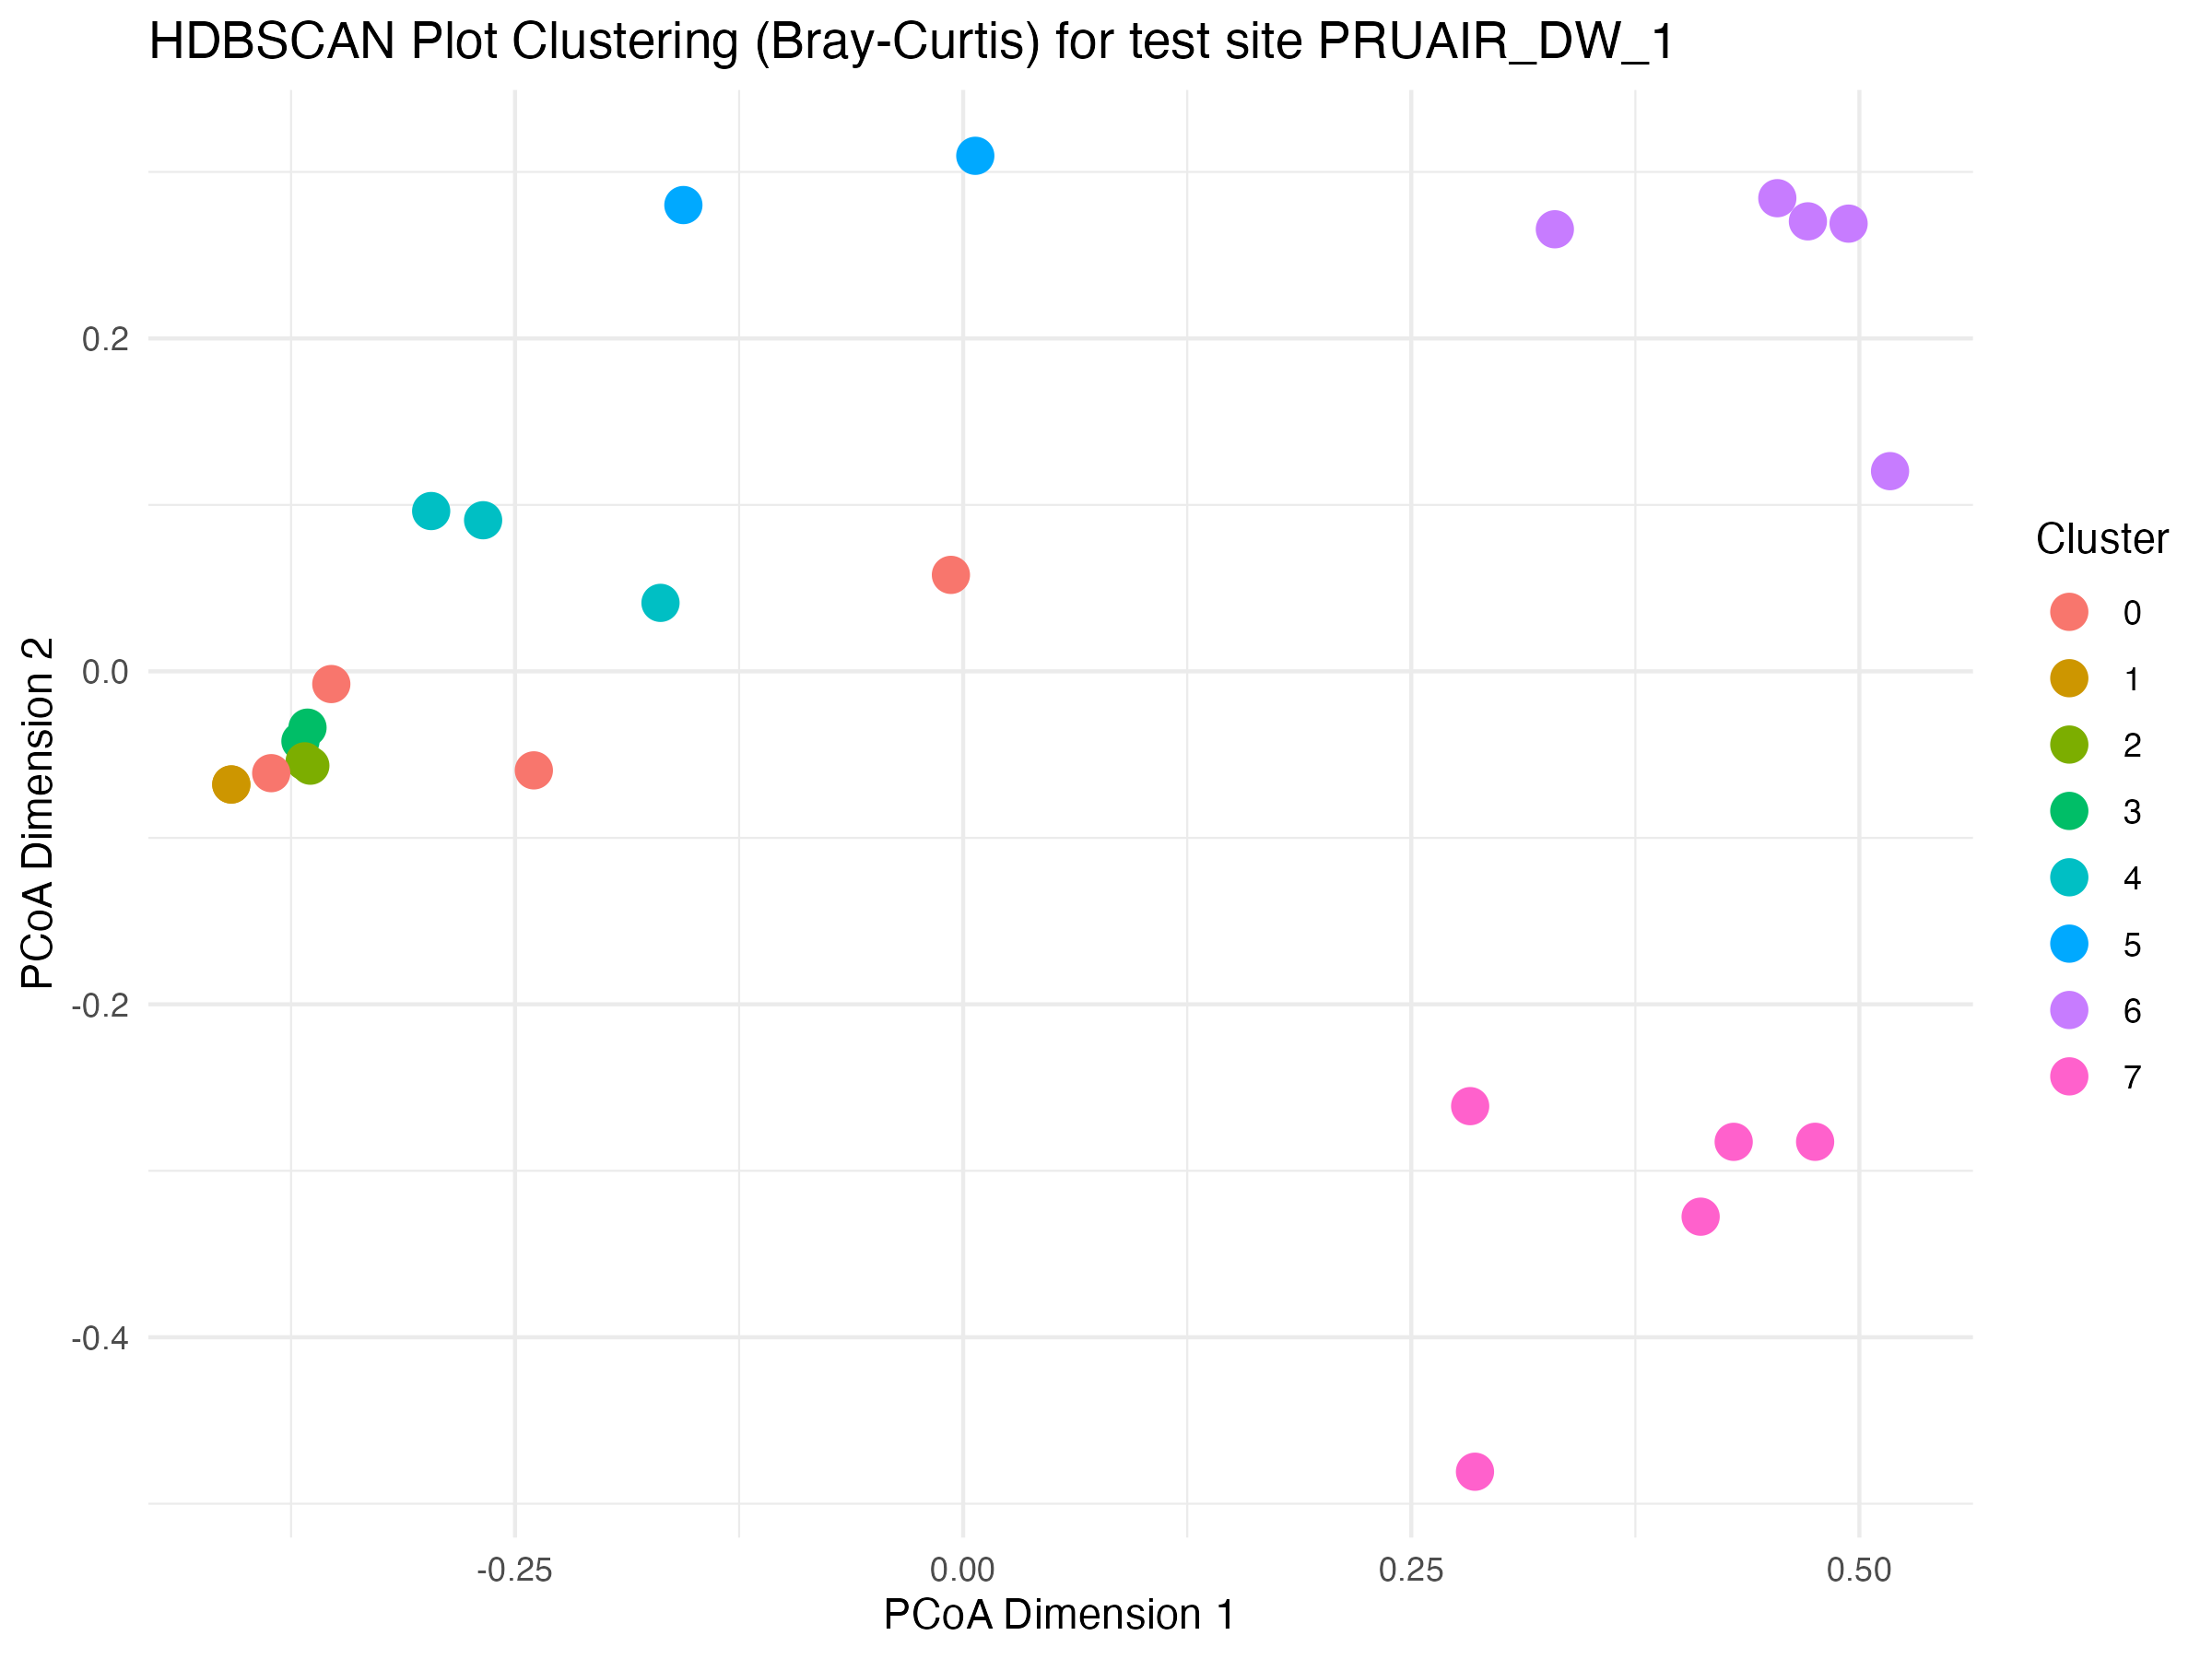
\includegraphics[width=\textwidth]{Figures/Appendix/PlantCommunityClustering/PRUAIR_DW_1_HDBSCAN_clusters.png}
%         \caption{PRUAIR\_DW\_1}
%         \label{fig:PRUAIR_DW_1_HDBSCAN_clusters}
%     \end{minipage}
%     \hfill
%     \begin{minipage}[b]{0.45\textwidth}
%         \centering
%         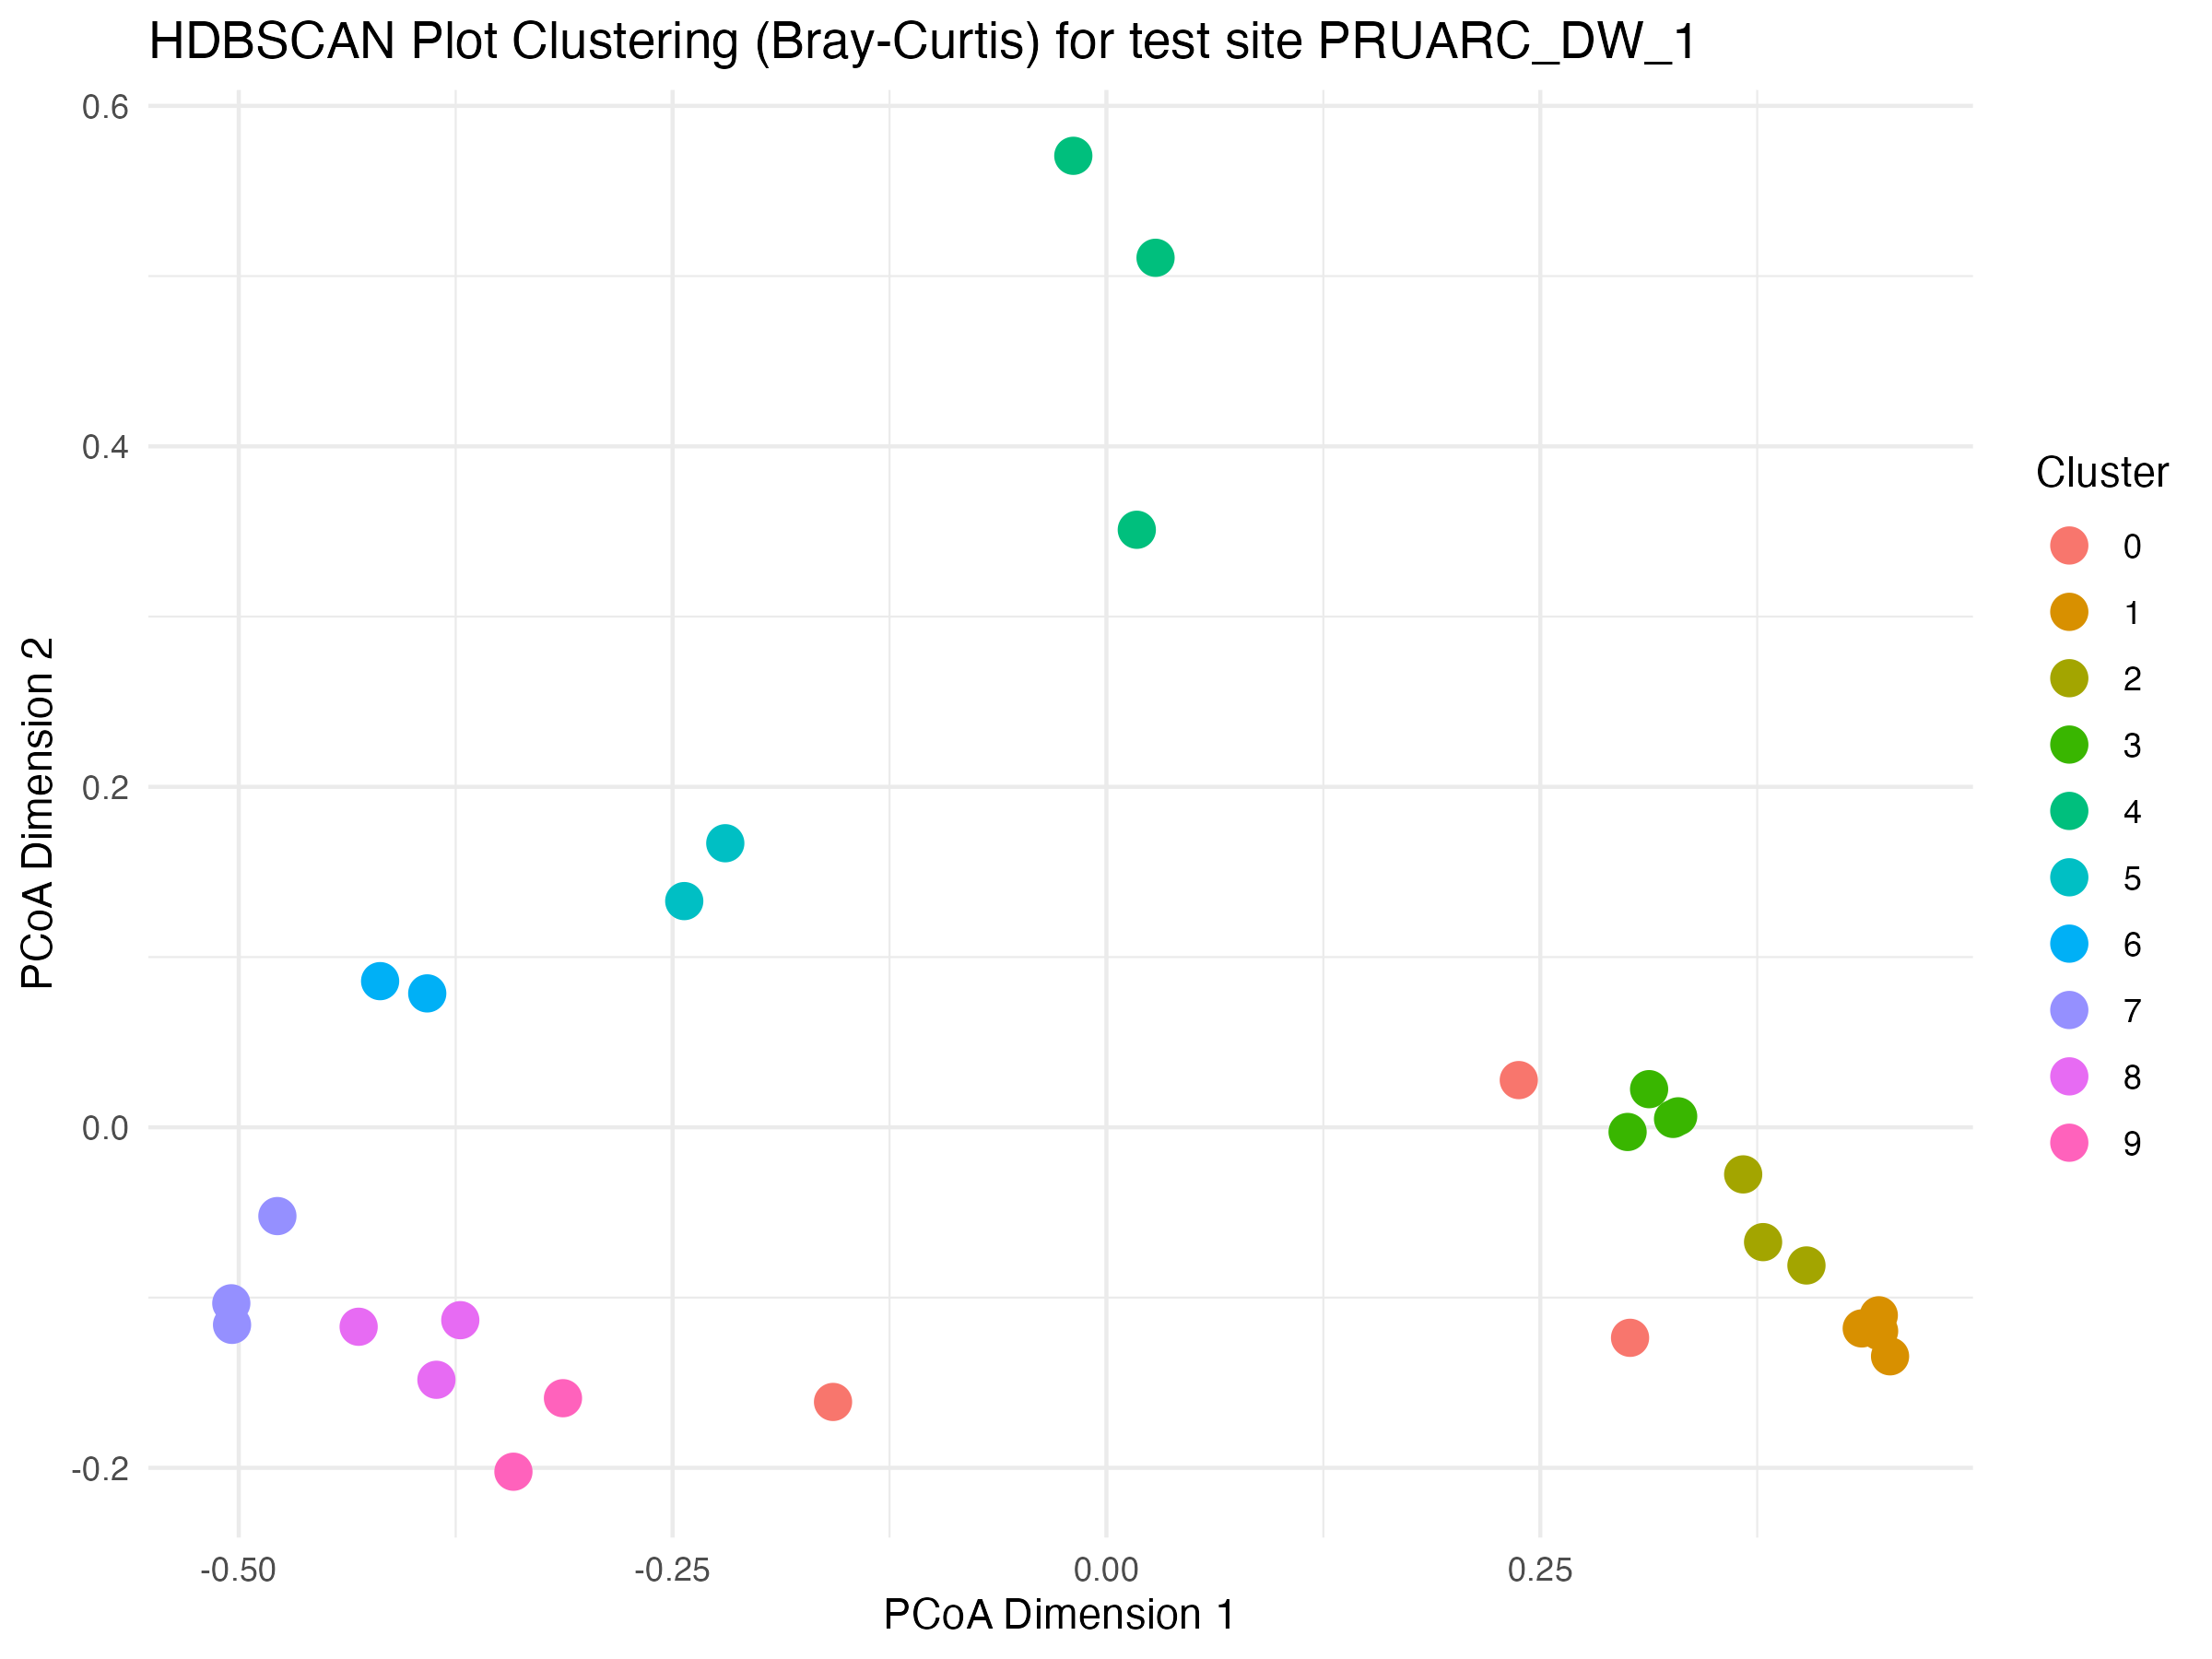
\includegraphics[width=\textwidth]{Figures/Appendix/PlantCommunityClustering/PRUARC_DW_1_HDBSCAN_clusters.png}
%         \caption{PRUARC\_DW\_1}
%         \label{fig:PRUARC_DW_1_HDBSCAN_clusters}
%     \end{minipage}
%     \captionof{figure}{Community Cluster Plots for Test Sites FRST\_AK\_2, FRST\_AK\_3, PRUAIR\_DW\_1, and PRUARC\_DW\_1}
%     \label{fig:group3_clusters}
% \end{figure}

\chapter{Linear Regression Models} % Main appendix title

\label{Appendix_LinearRegression}


\section{Plant species - spectral species}

\subsection{Results over all test sites}

\begin{table}[ht]
\centering
\caption{Summary of linear regression model predicting plant species richness from spectral species richness over all test sites}
\begin{tabular}{lcccc}
\hline
\textbf{Predictor} & \textbf{Estimate} & \textbf{Std. Error} & \textbf{t value} & \textbf{Pr($>$$|$t$|$)} \\
\hline
Intercept & 57.2577 & 18.1108 & 3.162 & \textbf{0.00905**} \\
Unique Spectral Species & 0.5489 & 0.6323 & 0.868 & 0.40390 \\
\hline
\multicolumn{5}{l}{\textit{Residual standard error:} 33.38 on 11 degrees of freedom} \\
\multicolumn{5}{l}{\textit{Multiple R-squared:} 0.06411 \quad \textit{Adjusted R-squared:} -0.02097} \\
\multicolumn{5}{l}{\textit{F-statistic:} 0.7535 on 1 and 11 DF, \quad \textit{p-value:} 0.4039} \\
\hline
\end{tabular}
\label{tab:lm_plantspecies_spectral}
\end{table}

\begin{figure}[H]
    \centering
    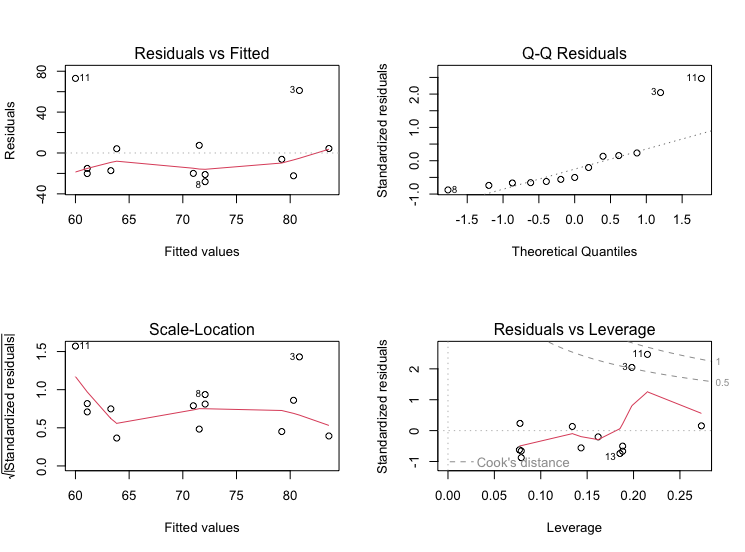
\includegraphics[width=0.9\textwidth]{Figures/Appendix/LRM_Plots/all_model_plant_species_lm.png} % Replace with your actual image path
    \caption{Residual plots for the linear regression model to predict pant species numbers from spectral species over all plots. Clear outliers are detectable in the residual vs fitted and the Q-Q residual plot (3 and 11)}
    \label{fig:all_model_plant_species_lm}
\end{figure}

\subsection{Results for Group C/D}
\begin{table}[ht]
\centering
\caption{Summary of linear regression model predicting plant species richness from spectral species richness for Group C/D}
\begin{tabular}{lcccc}
\hline
\textbf{Predictor} & \textbf{Estimate} & \textbf{Std. Error} & \textbf{t value} & \textbf{Pr($>$$|$t$|$)} \\
\hline
Intercept & 62.2493 & 25.3566 & 2.455 & \textbf{0.0396*} \\
Unique Spectral Species & 0.3982 & 0.8102 & 0.491 & 0.6363 \\
\hline
\multicolumn{5}{l}{\textit{Residual standard error:} 38.28 on 8 degrees of freedom} \\
\multicolumn{5}{l}{\textit{Multiple R-squared:} 0.02931 \quad \textit{Adjusted R-squared:} -0.09203} \\
\multicolumn{5}{l}{\textit{F-statistic:} 0.2416 on 1 and 8 DF, \quad \textit{p-value:} 0.6363} \\
\hline
\end{tabular}
\label{tab:lm_plantspecies_spectral_group_cd}
\end{table}

\begin{figure}[H]
    \centering
    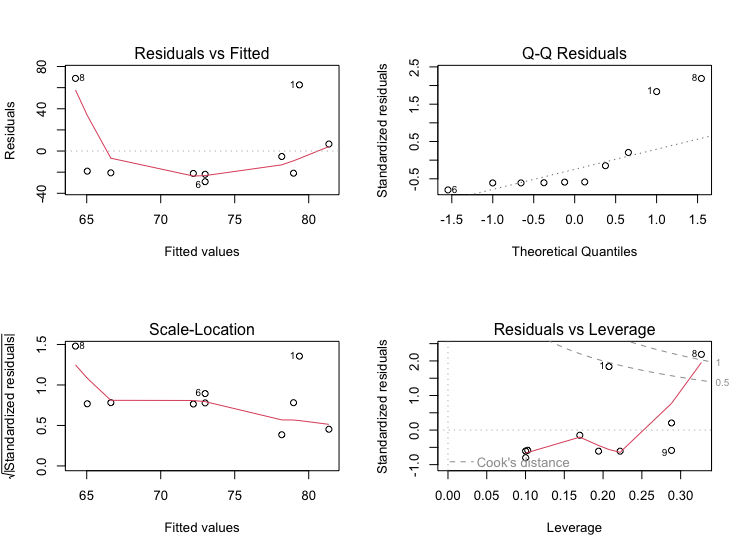
\includegraphics[width=0.9\textwidth]{Figures/Appendix/LRM_Plots/group_c_d_model_plant_species_lm.png} % Replace with your actual image path
    \caption{Residual plots for the linear regression model to predict plant species numbers from spectral species in group C/D. Clear outliers are detectable in the residual vs fitted and the Q-Q residual plot (1 and 8)}
    \label{fig:group_c_d_model_plant_species_lm}
\end{figure}

\subsection{Results for Group E}
\begin{table}[ht]
\centering
\caption{Summary of linear regression model predicting plant species richness from spectral species richness for Group E}
\begin{tabular}{lcccc}
\hline
\textbf{Predictor} & \textbf{Estimate} & \textbf{Std. Error} & \textbf{t value} & \textbf{Pr($>$$|$t$|$)} \\
\hline
Intercept & 36.6100 & 16.3602 & 2.238 &  0.268 \\
Unique Spectral Species & 1.7371 & 0.9613 & 1.807 & 0.322 \\
\hline
\multicolumn{5}{l}{\textit{Residual standard error:} 13.39 on 1 degrees of freedom} \\
\multicolumn{5}{l}{\textit{Multiple R-squared:} 0.7656 \quad \textit{Adjusted R-squared:} 0.5311} \\
\multicolumn{5}{l}{\textit{F-statistic:} 3.266 on 1 and 1 DF, \quad \textit{p-value:} 0.3218} \\
\hline
\end{tabular}
\label{tab:lm_plantspecies_spectral_group_e}
\end{table}

\begin{figure}[H]
    \centering
    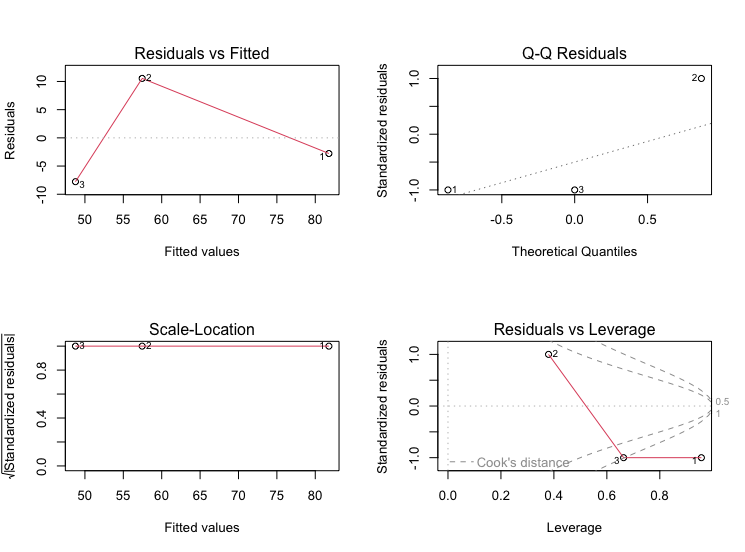
\includegraphics[width=0.9\textwidth]{Figures/Appendix/LRM_Plots/group_e_model_plant_species_lm.png} % Replace with your actual image path
    \caption{Residual plots for the linear regression model to predict plant species numbers from spectral species in group E. Since there are so few data points the the results don't hold any value.}
    \label{fig:group_e_model_plant_species_lm}
\end{figure}


\section{Plant communities - spectral species}
\subsection{Results over all test sites}
\begin{table}[ht]
\centering
\caption{Summary of linear regression model predicting plant community richness from spectral species richness over all test sites}
\begin{tabular}{lcccc}
\hline
\textbf{Predictor} & \textbf{Estimate} & \textbf{Std. Error} & \textbf{t value} & \textbf{Pr($>$$|$t$|$)} \\
\hline
Intercept & 9.08876 & 2.53324 & 3.588 & \textbf{0.00426**} \\
Unique Spectral Species & -0.02236 & 0.08845 & -0.253 & 0.80512 \\
\hline
\multicolumn{5}{l}{\textit{Residual standard error:} 4.669 on 11 degrees of freedom} \\
\multicolumn{5}{l}{\textit{Multiple R-squared:} 0.005774 \quad \textit{Adjusted R-squared:} -0.08461} \\
\multicolumn{5}{l}{\textit{F-statistic:} 0.06389 on 1 and 11 DF, \quad \textit{p-value:} 0.8051} \\
\hline
\end{tabular}
\label{tab:lm_plant_community_spectral}
\end{table}

\begin{figure}[H]
    \centering
    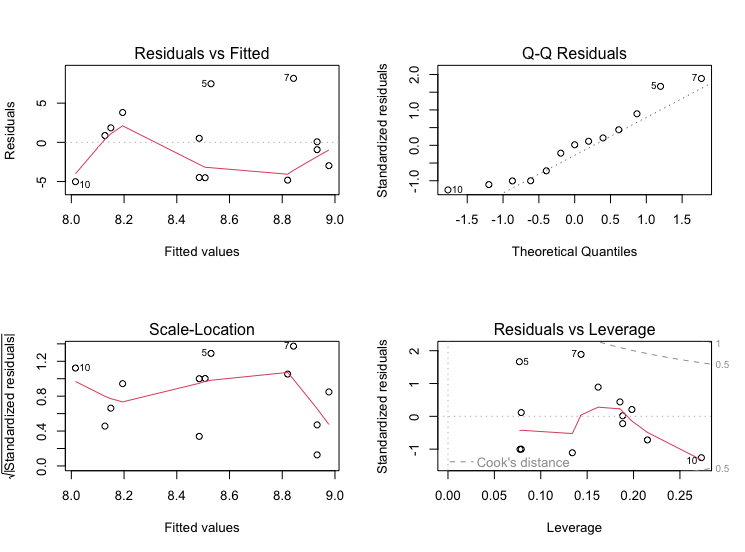
\includegraphics[width=0.9\textwidth]{Figures/Appendix/LRM_Plots/all_model_plant_communities_lm.png} % Replace with your actual image path
    \caption{Residual plots for the linear regression model to predict plant community numbers from spectral species over all plots.}
    \label{fig:all_model_plant_communities_lm}
\end{figure}

\subsection{Results for Group C/D}
\begin{table}[ht]
\centering
\caption{Summary of linear regression model predicting plant community richness from spectral species richness for Group C/D}
\begin{tabular}{lcccc}
\hline
\textbf{Predictor} & \textbf{Estimate} & \textbf{Std. Error} & \textbf{t value} & \textbf{Pr($>$$|$t$|$)} \\
\hline
Intercept & 11.00134 & 3.18381 & 3.455 & \textbf{0.00863**} \\
Unique Spectral Species & -0.05823 & 0.10173 & -0.572 & 0.58277 \\
\hline
\multicolumn{5}{l}{\textit{Residual standard error:} 4.807 on 8 degrees of freedom} \\
\multicolumn{5}{l}{\textit{Multiple R-squared:} 0.03935 \quad \textit{Adjusted R-squared:} -0.08074} \\
\multicolumn{5}{l}{\textit{F-statistic:} 0.3277 on 1 and 8 DF, \quad \textit{p-value:} 0.5828} \\
\hline
\end{tabular}
\label{tab:lm_plantspecies_spectral}
\end{table}

\begin{figure}[H]
    \centering
    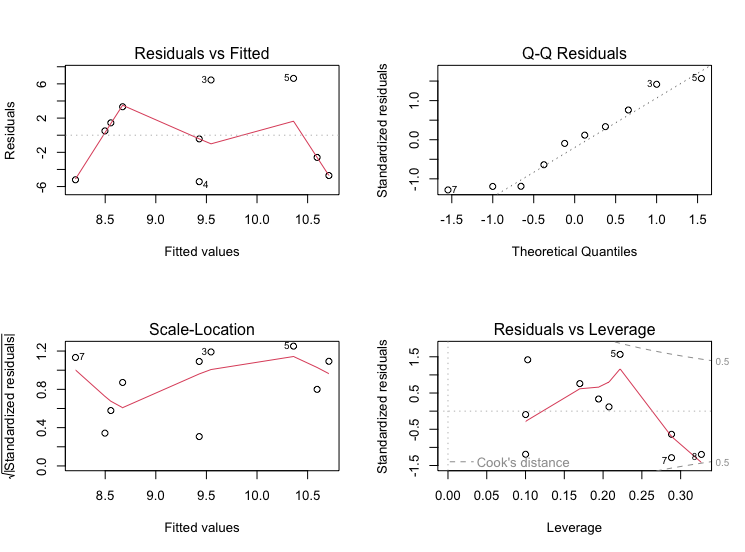
\includegraphics[width=0.9\textwidth]{Figures/Appendix/LRM_Plots/group_c_d_model_plant_communities_lm.png} % Replace with your actual image path
    \caption{Residual plots for the linear regression model to predict plant community numbers from spectral species in group C/D.}
    \label{fig:group_c_d_model_plant_communities_lm}
\end{figure}

\subsection{Results for Group E}
\begin{table}[ht]
\centering
\caption{Summary of linear regression model predicting plant community richness from spectral species richness for Group E}
\begin{tabular}{lcccc}
\hline
\textbf{Predictor} & \textbf{Estimate} & \textbf{Std. Error} & \textbf{t value} & \textbf{Pr($>$$|$t$|$)} \\
\hline
Intercept & 8.7595 & 3.5456 & 2.471 & 0.245 \\
Unique Spectral Species & -0.2062 & 0.2083 & -0.990 & 0.503 \\
\hline
\multicolumn{5}{l}{\textit{Residual standard error:} 2.902 on 1 degrees of freedom} \\
\multicolumn{5}{l}{\textit{Multiple R-squared:} 0.4948 \quad \textit{Adjusted R-squared:} -0.01031} \\
\multicolumn{5}{l}{\textit{F-statistic:} 0.9796 on 1 and 1 DF, \quad \textit{p-value:} 0.5033} \\
\hline
\end{tabular}
\label{tab:lm_plantspecies_spectral}
\end{table}

\begin{figure}[H]
    \centering
    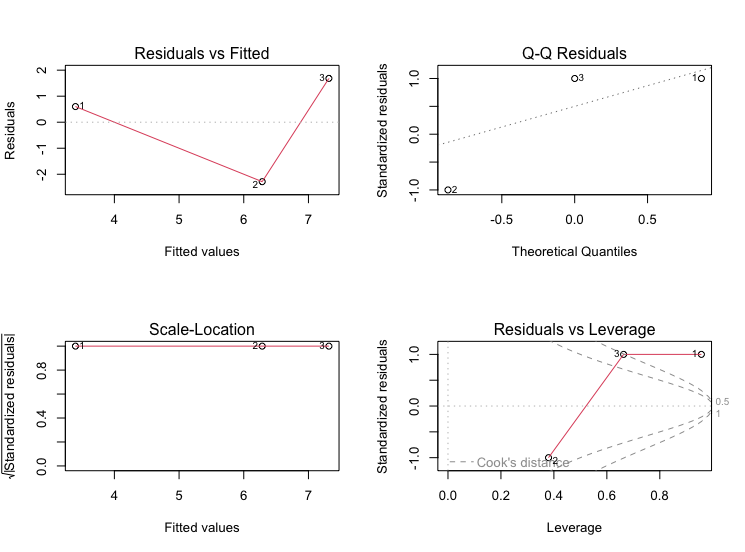
\includegraphics[width=0.9\textwidth]{Figures/Appendix/LRM_Plots/group_e_model_plant_communities_lm.png} % Replace with your actual image path
    \caption{Residual plots for the linear regression model to predict plant community numbers from spectral species in group E.}
    \label{fig:group_e_model_plant_communities_lm}
\end{figure}

\section{Habitat types - spectral species}
\begin{table}[ht]
\centering
\caption{Summary of linear regression model predicting habitat type richness from spectral species richness over all test sites}
\begin{tabular}{lcccc}
\hline
\textbf{Predictor} & \textbf{Estimate} & \textbf{Std. Error} & \textbf{t value} & \textbf{Pr($>$$|$t$|$)} \\
\hline
Intercept & 2.94635 & 0.86879 & 3.391 & \textbf{0.00602**} \\
Unique Spectral Species & 0.03030 & 0.03033 & 0.999 & 0.33925 \\
\hline
\multicolumn{5}{l}{\textit{Residual standard error:} 1.601 on 11 degrees of freedom} \\
\multicolumn{5}{l}{\textit{Multiple R-squared:} 0.08319 \quad \textit{Adjusted R-squared:} -0.0001603} \\
\multicolumn{5}{l}{\textit{F-statistic:} 0.9981 on 1 and 11 DF, \quad \textit{p-value:} 0.3392} \\
\hline
\end{tabular}
\label{tab:lm_habitat_type_spectral}
\end{table}

\begin{figure}[H]
    \centering
    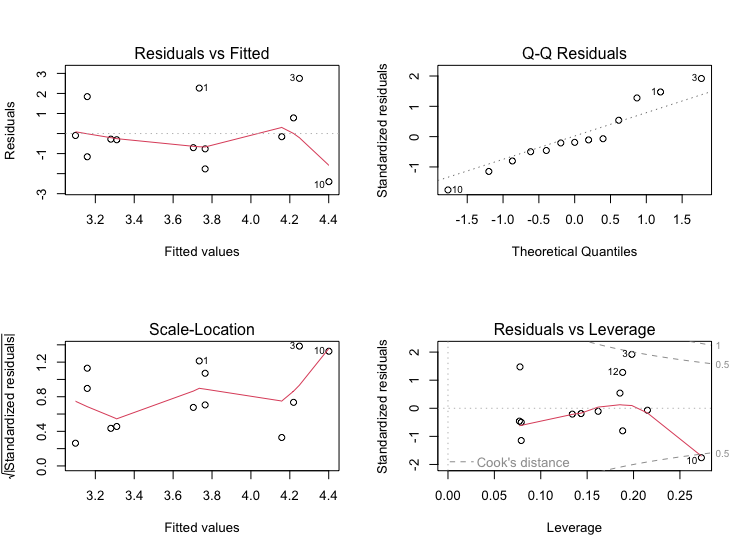
\includegraphics[width=0.9\textwidth]{Figures/Appendix/LRM_Plots/all_model_habitat_types_lm.png} % Replace with your actual image path
    \caption{Residual plots for the linear regression model to predict habitat type numbers from spectral species over all plots.}
    \label{fig:all_model_habitat_types_lm}
\end{figure}


\subsection{Results for Group C/D}
\begin{table}[ht]
\centering
\caption{Summary of linear regression model predicting habitat type richness from spectral species richness for Group C/D}
\begin{tabular}{lcccc}
\hline
\textbf{Predictor} & \textbf{Estimate} & \textbf{Std. Error} & \textbf{t value} & \textbf{Pr($>$$|$t$|$)} \\
\hline
Intercept & 3.17648 & 1.08058 & 2.940 & \textbf{0.0187*} \\
Unique Spectral Species & 0.01904 & 0.03453 & 0.551 & 0.5964 \\
\hline
\multicolumn{5}{l}{\textit{Residual standard error:} 1.631 on 8 degrees of freedom} \\
\multicolumn{5}{l}{\textit{Multiple R-squared:} 0.03661 \quad \textit{Adjusted R-squared:} -0.08381} \\
\multicolumn{5}{l}{\textit{F-statistic:} 0.304 on 1 and 8 DF, \quad \textit{p-value:} 0.5964} \\
\hline
\end{tabular}
\label{tab:lm_plantspecies_spectral}
\end{table}

\begin{figure}[H]
    \centering
    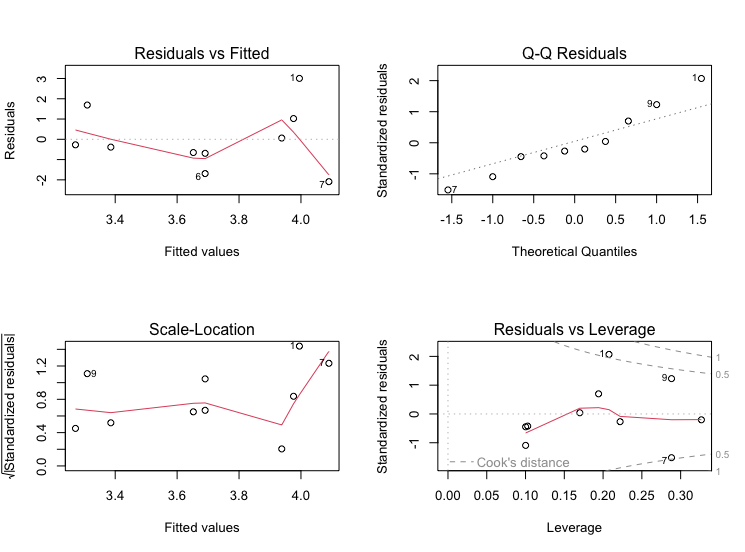
\includegraphics[width=0.9\textwidth]{Figures/Appendix/LRM_Plots/group_c_d_model_habitat_types_lm.png} % Replace with your actual image path
    \caption{Residual plots for the linear regression model to predict habitat type numbers from spectral species in group C/D.}
    \label{fig:group_c_d_model_habitat_types_lm}
\end{figure}

\subsection{Results for Group E}
\begin{table}[ht]
\centering
\caption{Summary of linear regression model predicting habitat type richness from spectral species richness for Group E}
\begin{tabular}{lcccc}
\hline
\textbf{Predictor} & \textbf{Estimate} & \textbf{Std. Error} & \textbf{t value} & \textbf{Pr($>$$|$t$|$)} \\
\hline
Intercept & 0.496564 & 0.050651 & 9.804 & 0.06471 \\
Unique Spectral Species & 0.211340 & 0.002976 & 71.014 & \textbf{0.00896**} \\
\hline
\multicolumn{5}{l}{\textit{Residual standard error:} 0.04145 on 1 degrees of freedom} \\
\multicolumn{5}{l}{\textit{Multiple R-squared:} 0.9998 \quad \textit{Adjusted R-squared:} 0.9996} \\
\multicolumn{5}{l}{\textit{F-statistic:} 5043 on 1 and 1 DF, \quad \textit{p-value:} 0.008964} \\
\hline
\end{tabular}
\label{tab:lm_plantspecies_spectral}
\end{table}

\begin{figure}[H]
    \centering
    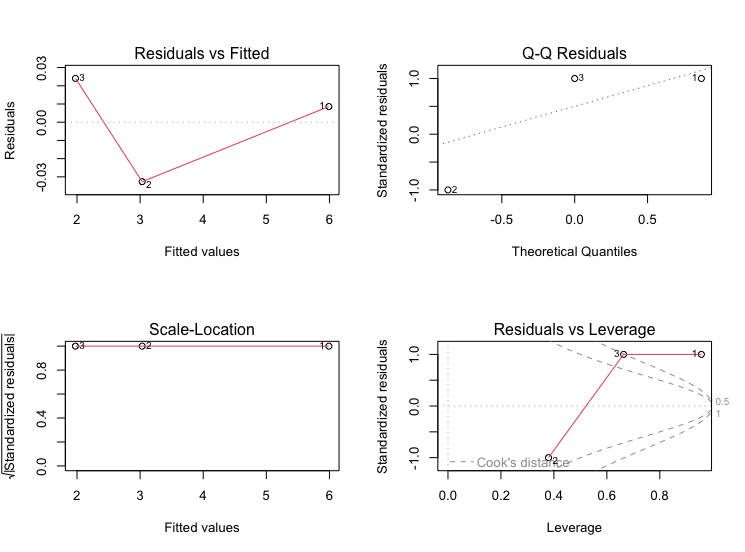
\includegraphics[width=0.9\textwidth]{Figures/Appendix/LRM_Plots/group_e_model_habitat_types_lm.png} % Replace with your actual image path
    \caption{Residual plots for the linear regression model to predict habitat type numbers from spectral species in group E.}
    \label{fig:group_e_model_habitat_types_lm}
\end{figure}
\chapter{Plant Community Clustering} % Main appendix title

\label{Appendix_PlantCommunityClustering}

\section{HDBSCAN cluster plots}

\subsection{AN\_TJ\_1}
\begin{figure}[H]
    \centering
    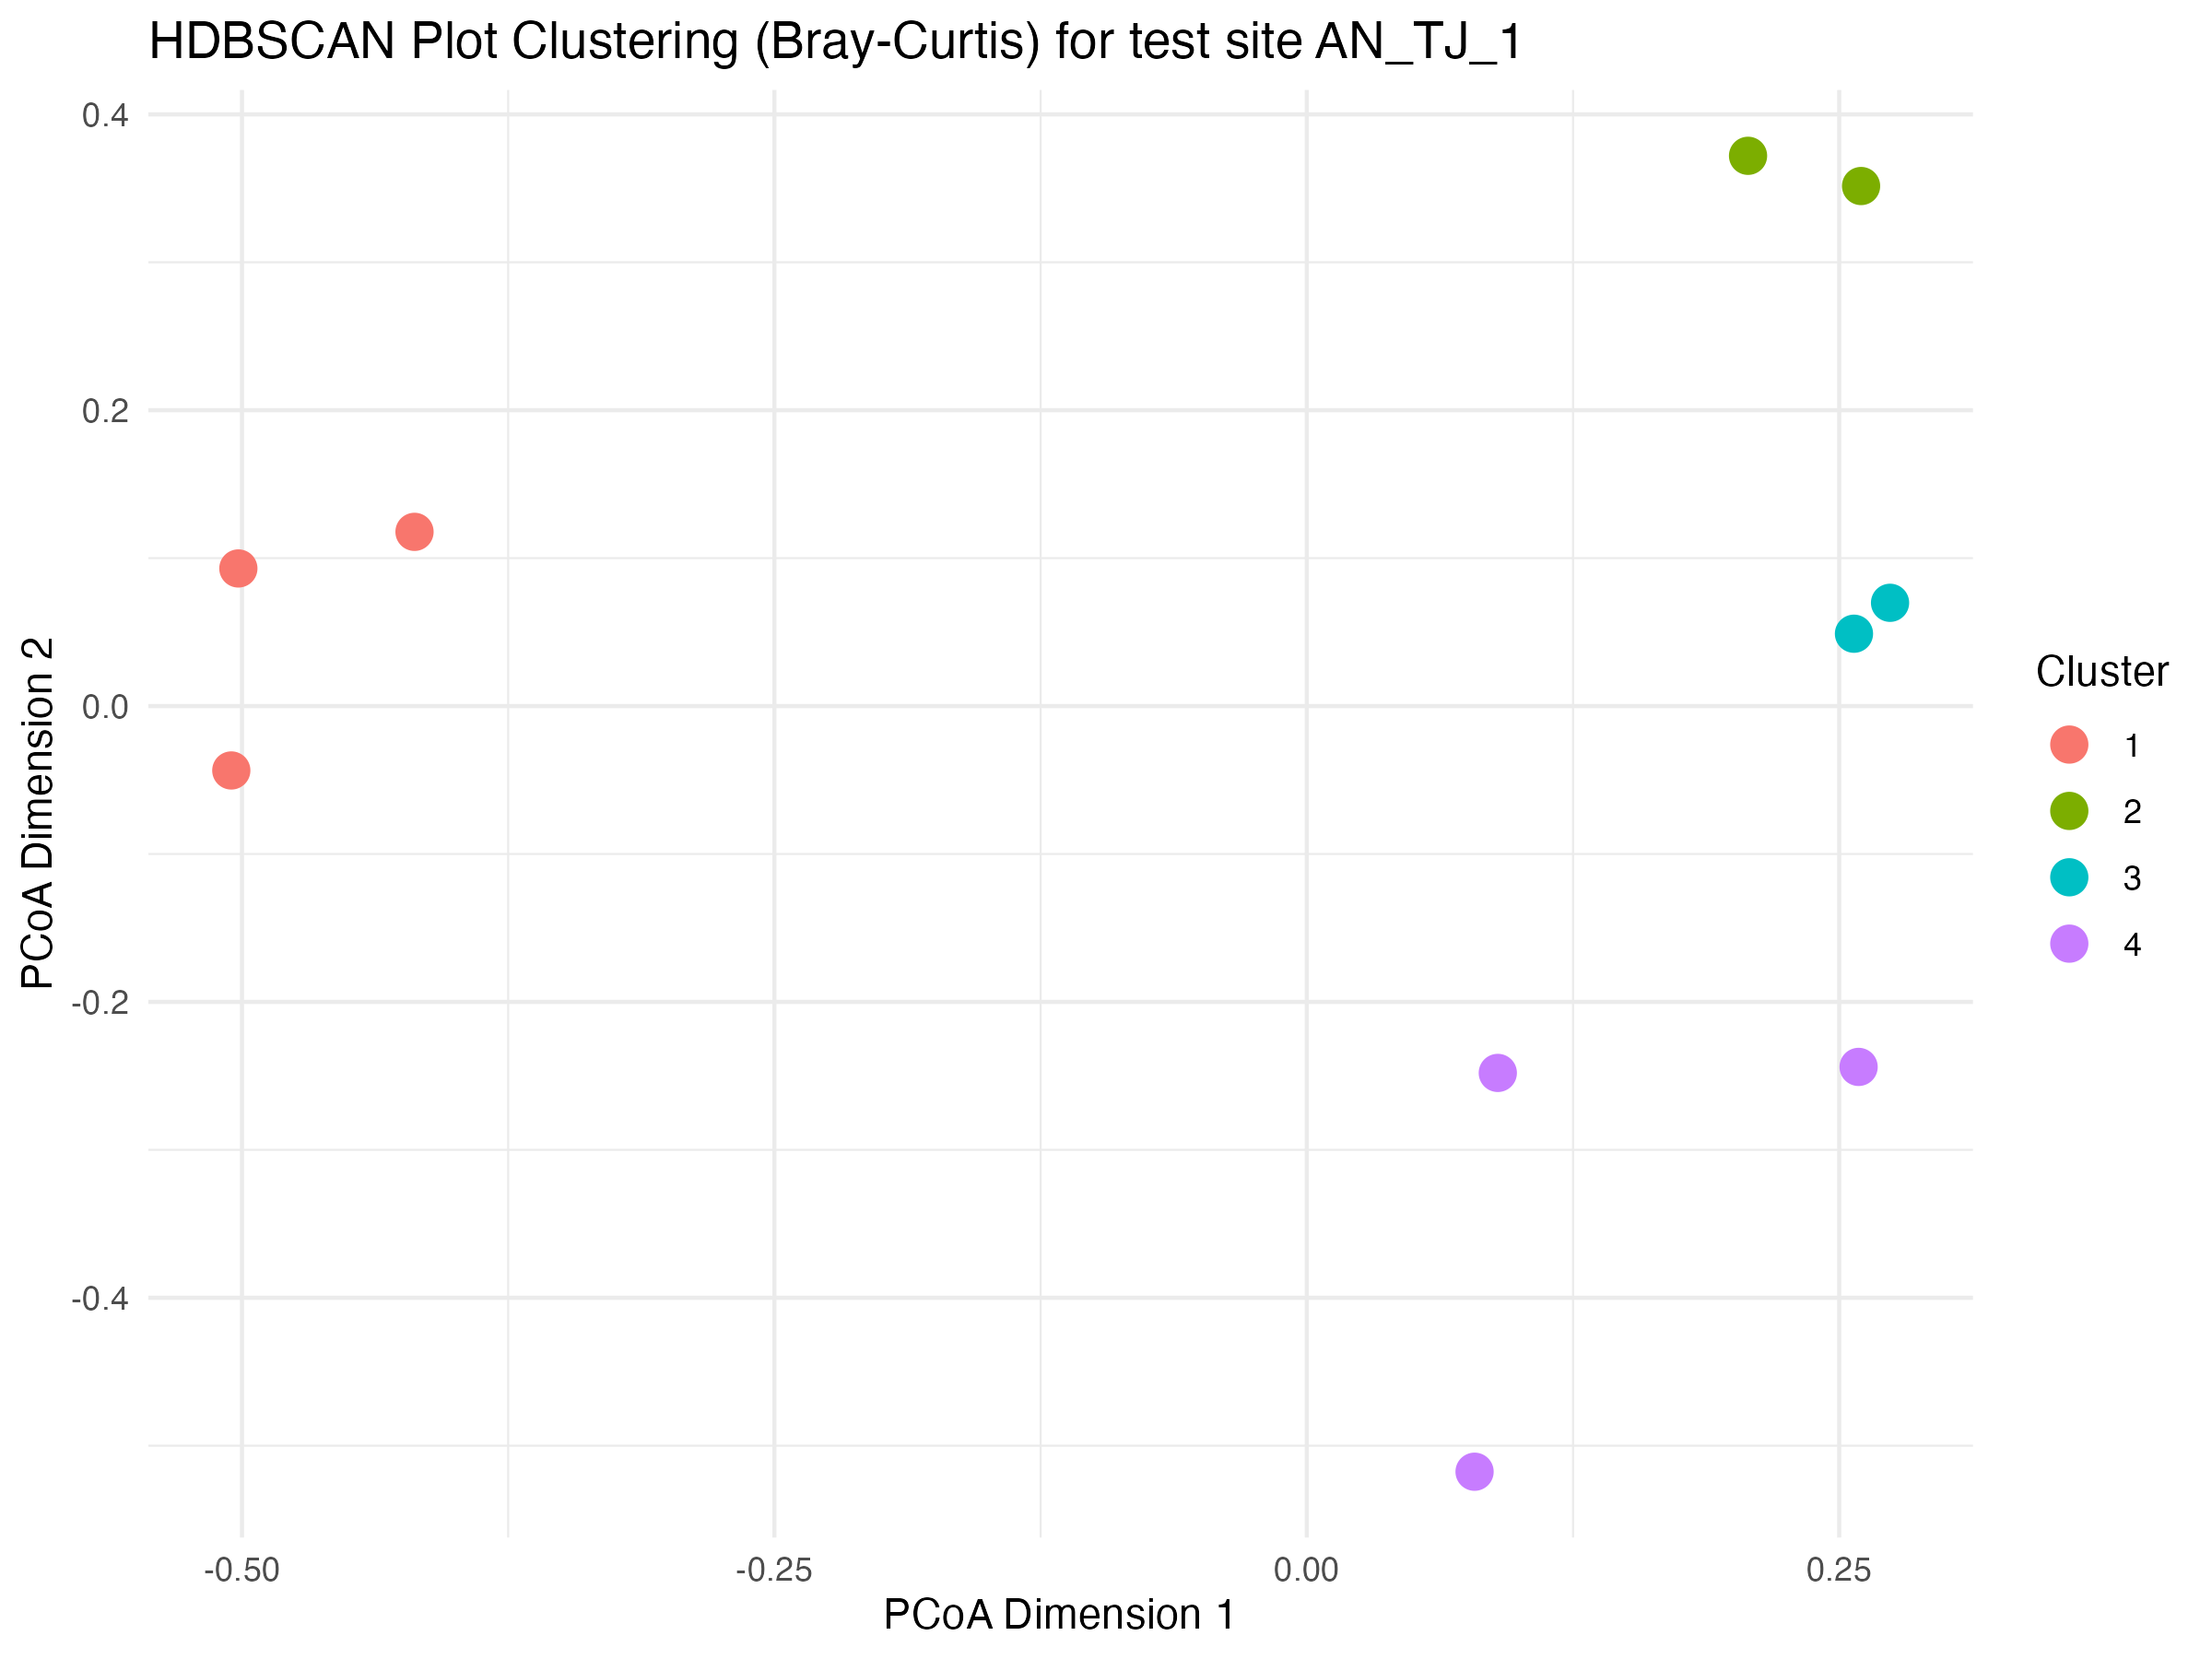
\includegraphics[width=0.9\textwidth]{Figures/Appendix/PlantCommunityClustering/AN_TJ_1_HDBSCAN_clusters.png} % Replace with your actual image path
    \caption{Community cluster HDBSCAN plot for test site AN\_TJ\_1}
    \label{fig:AN_TJ_1_HDBSCAN_clusters}
\end{figure}

\begin{figure}[H]
    \centering
    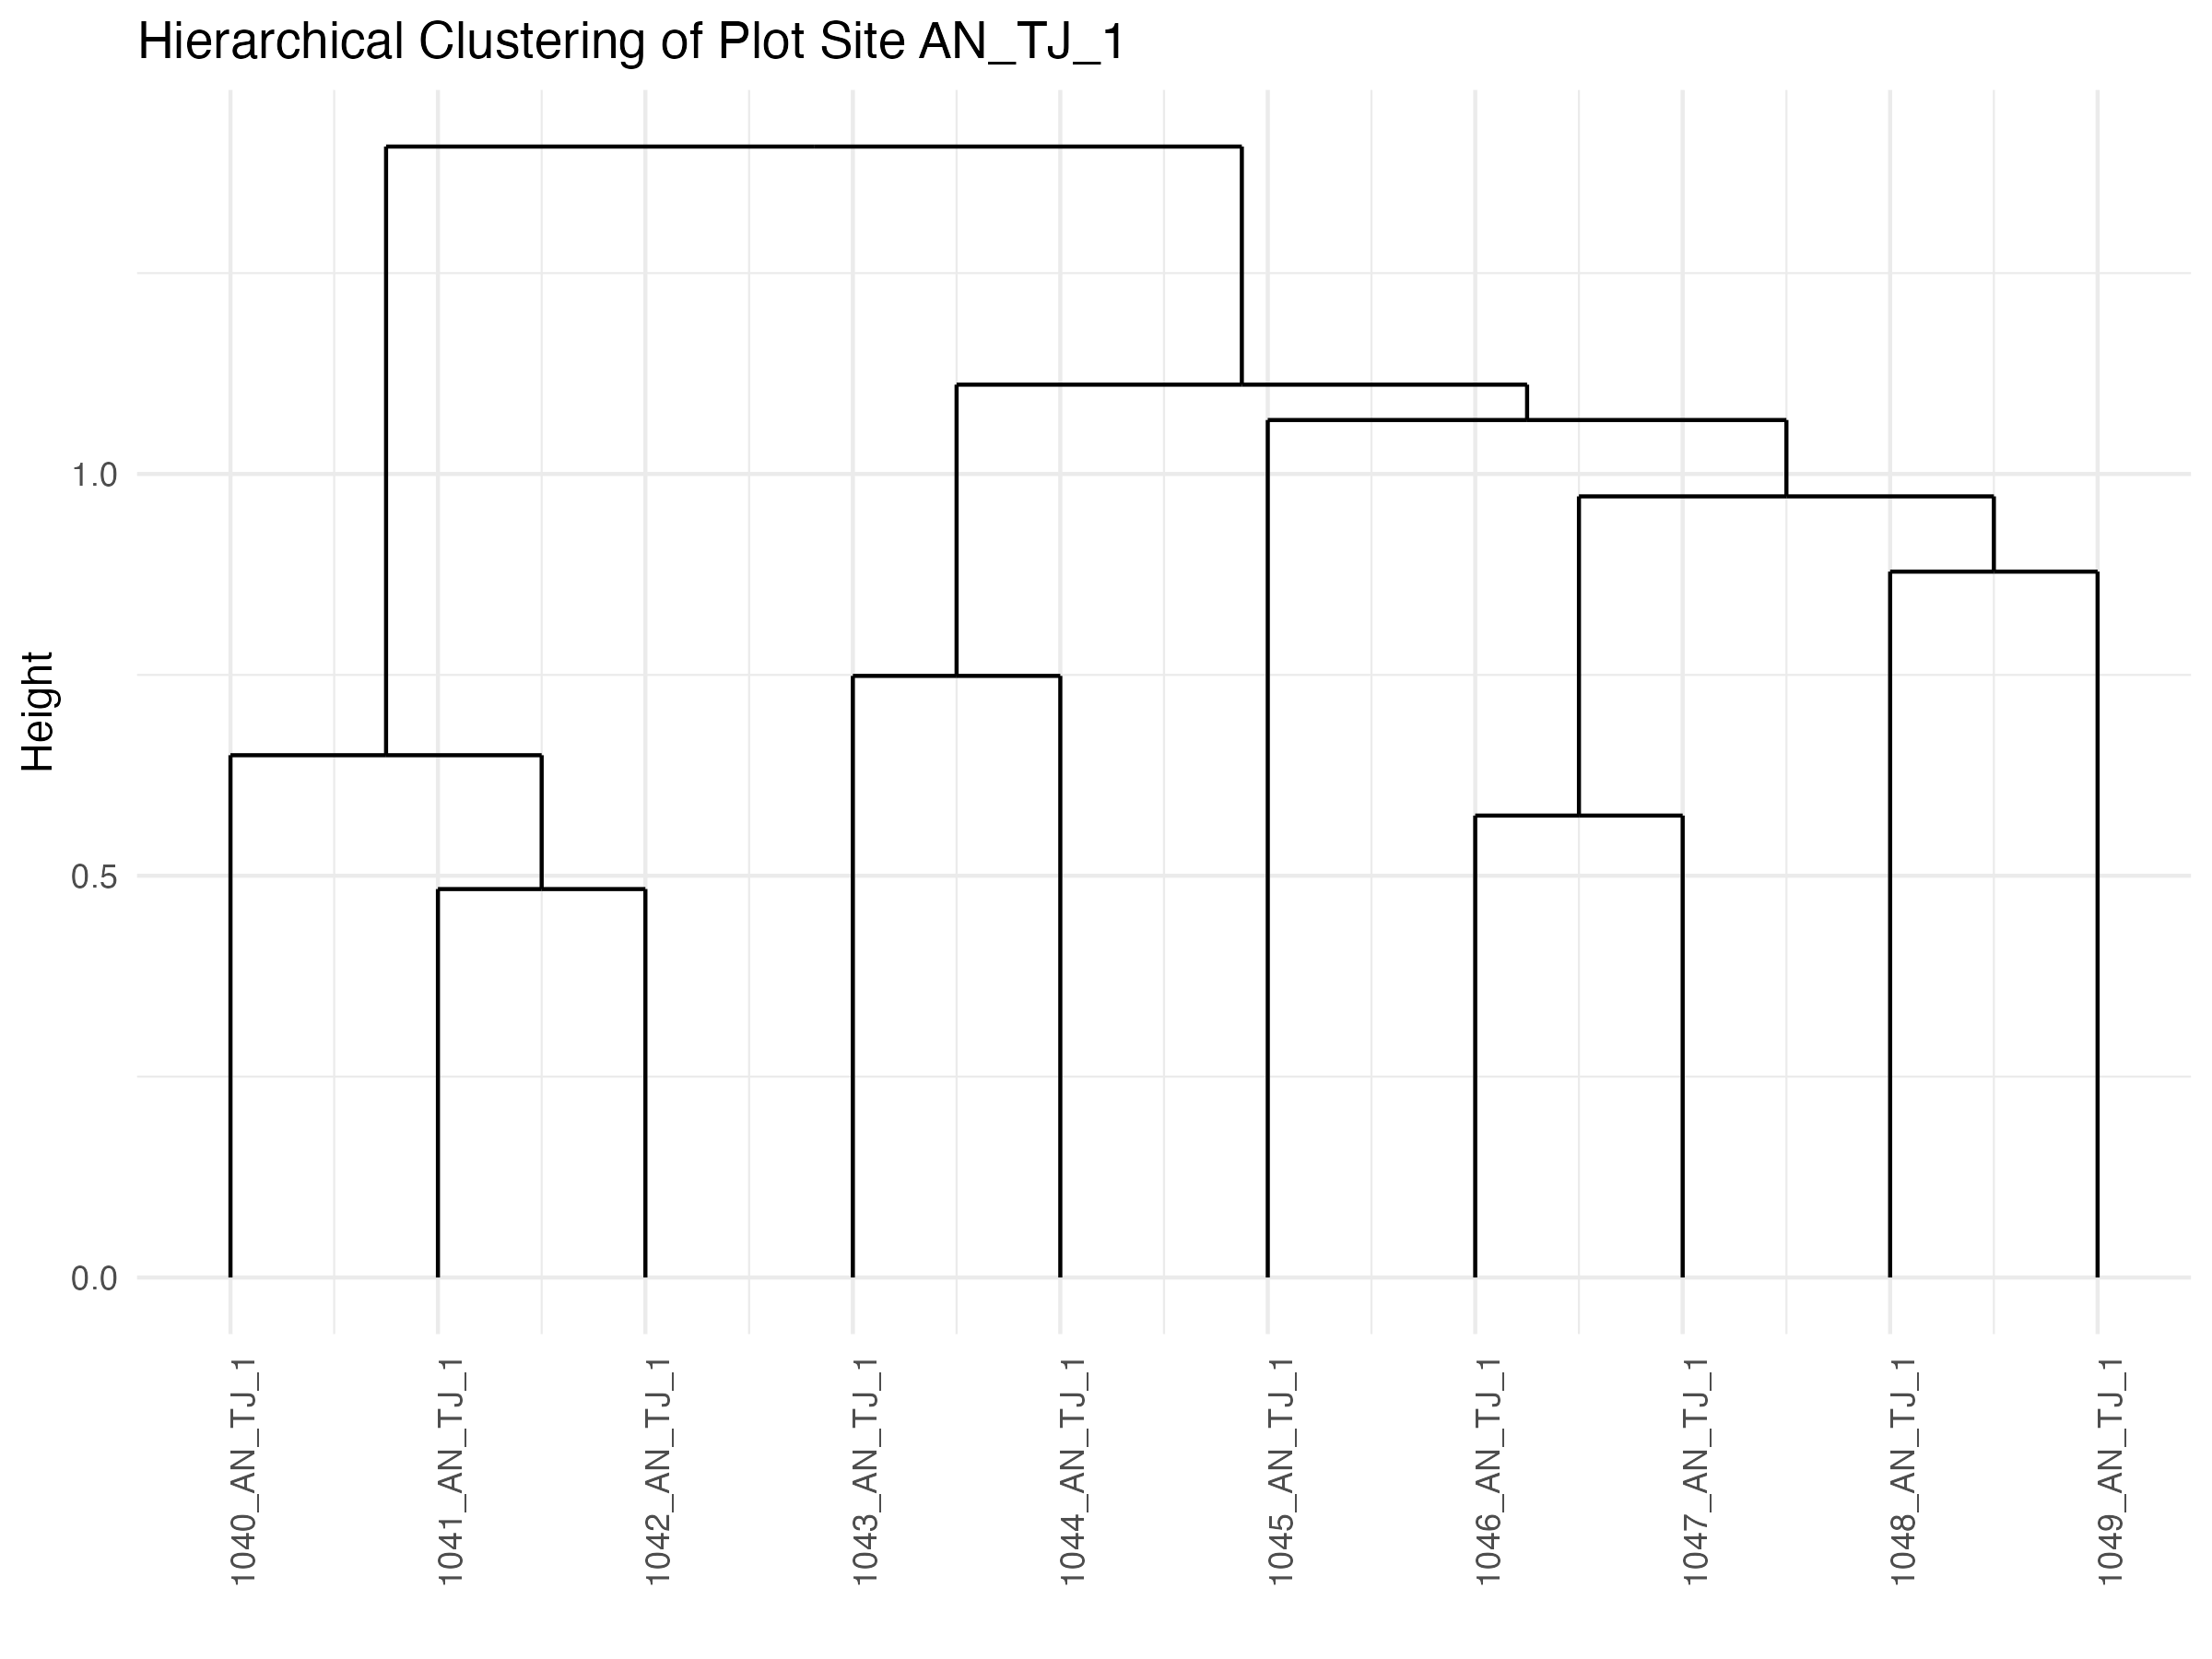
\includegraphics[width=0.9\textwidth]{Figures/Appendix/PlantCommunityClustering/AN_TJ_1_DENDRO.png} % Replace with your actual image path
    \caption{Community cluster dendrogram plot for test site AN\_TJ\_1}
    \label{fig:AN_TJ_1_DENDRO}
\end{figure}

\newpage

\subsection{AN\_TJ\_2}
\begin{figure}[H]
    \centering
    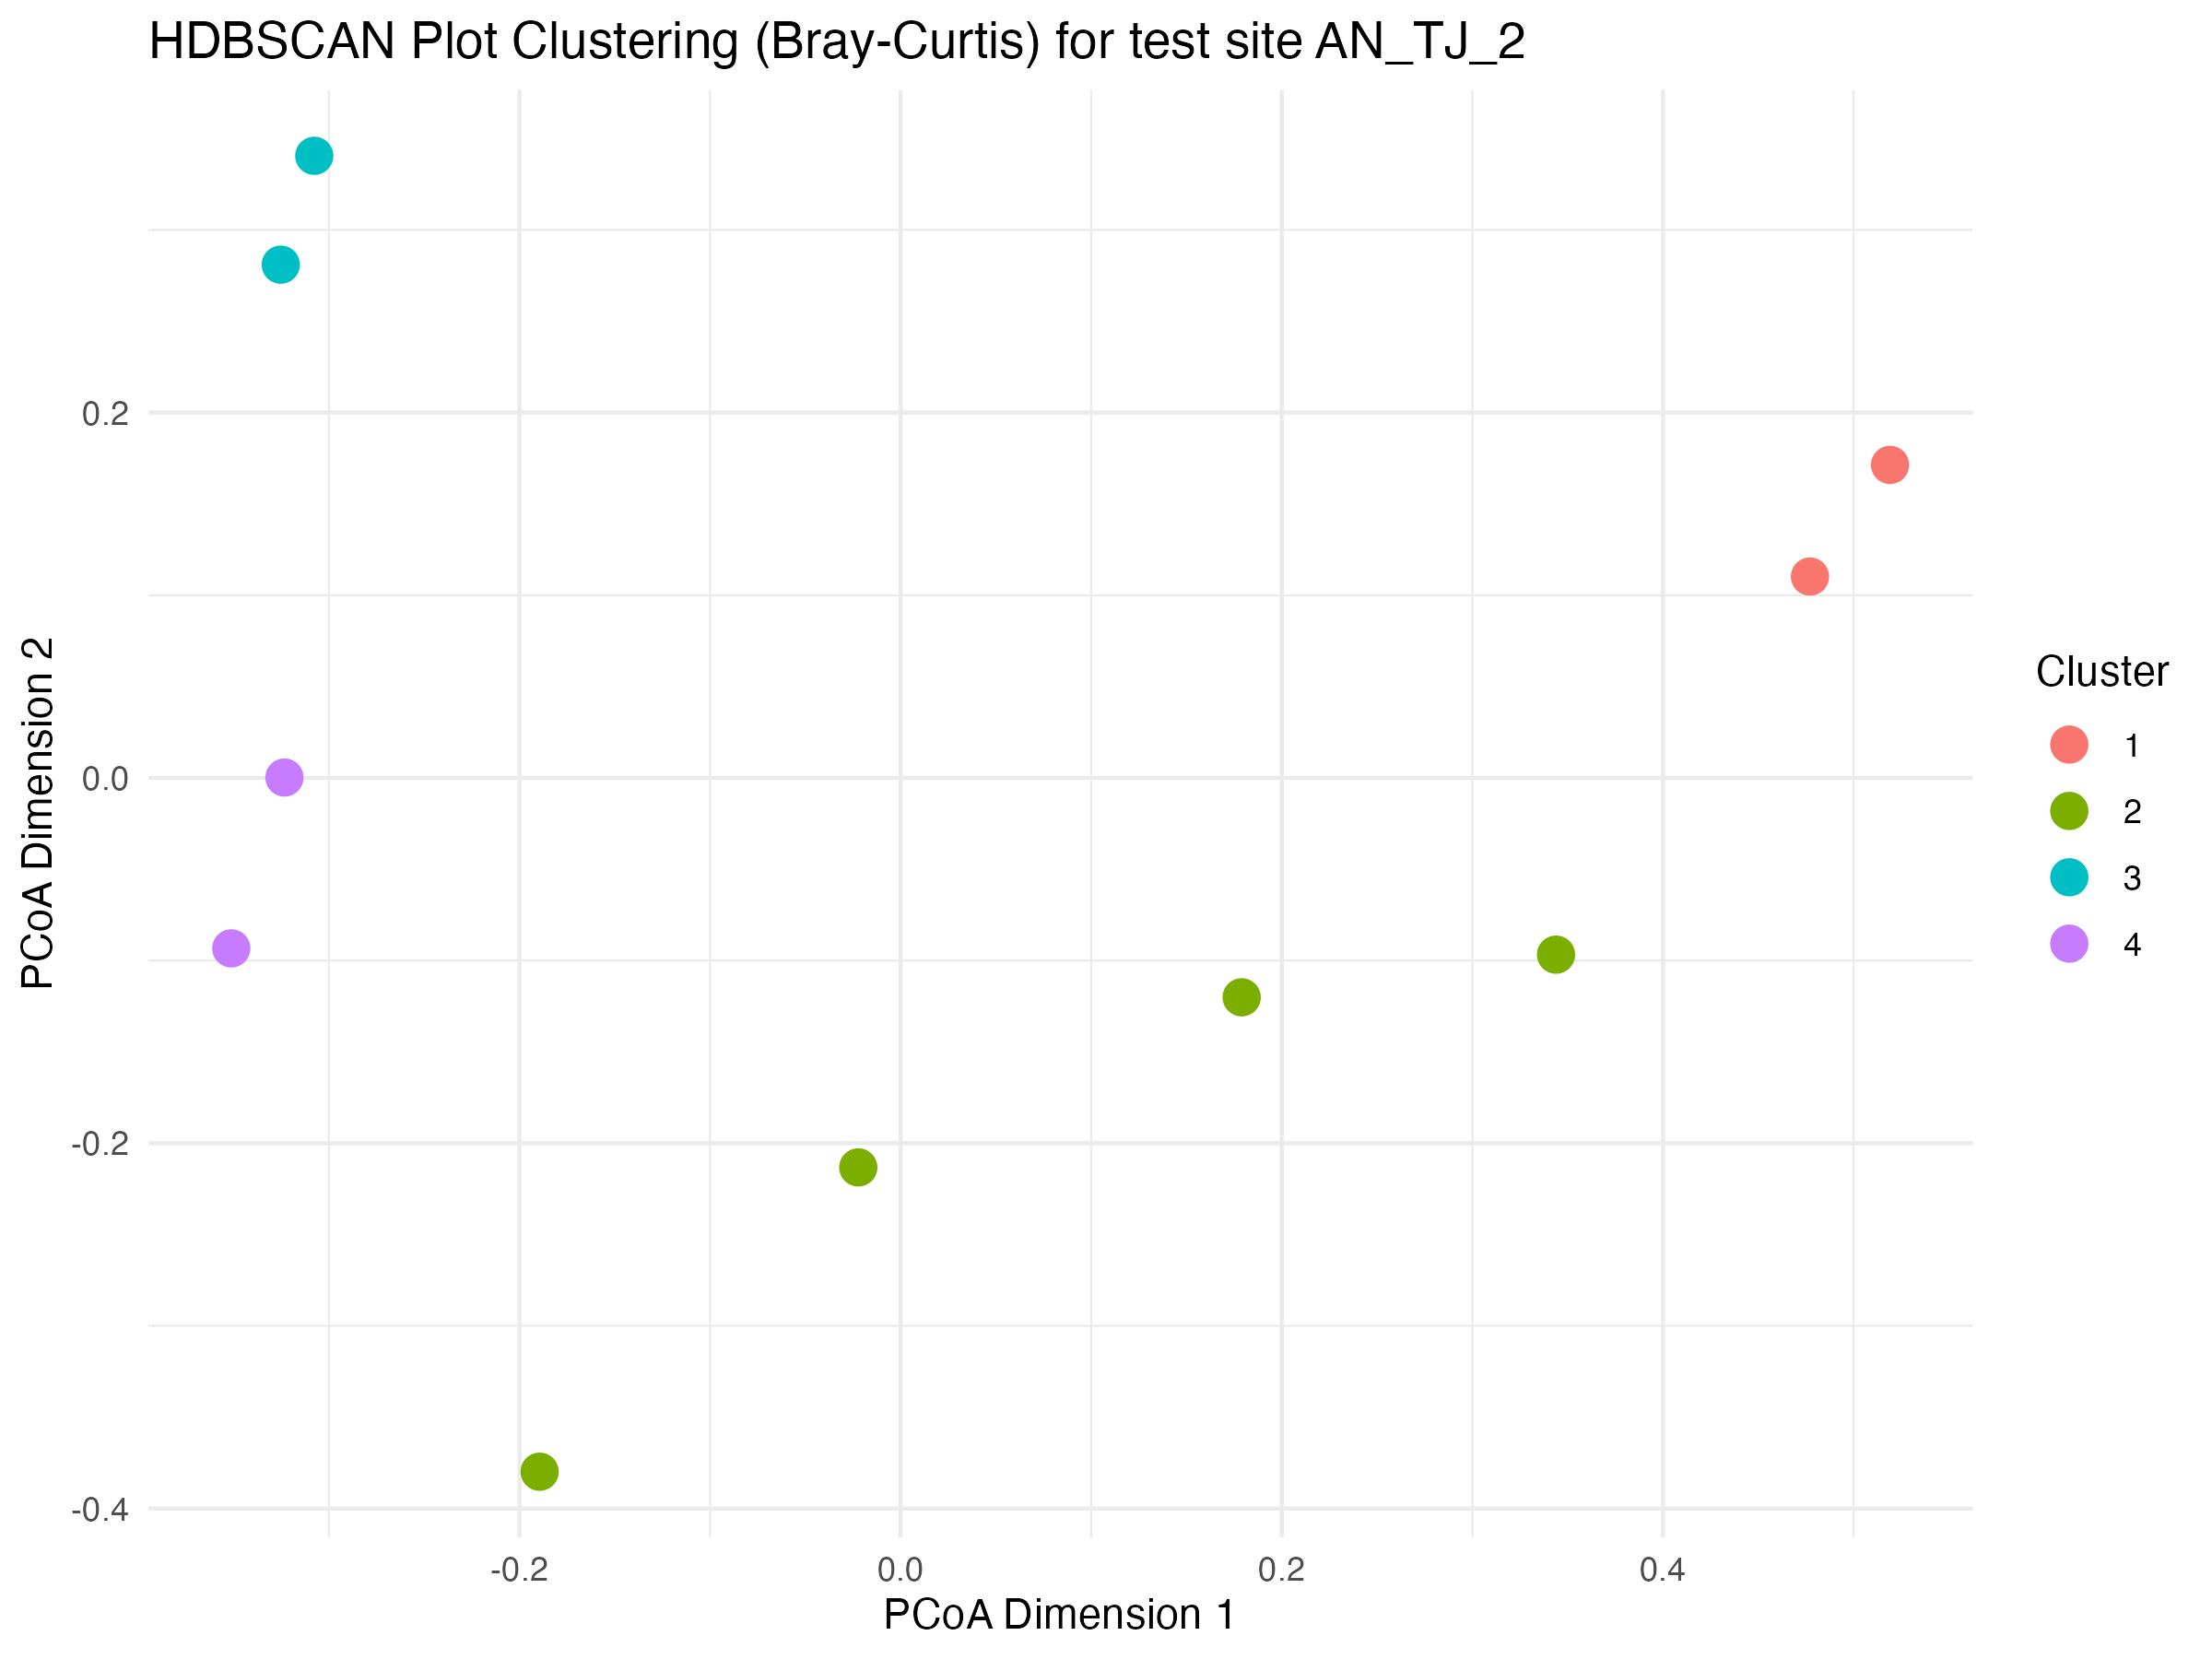
\includegraphics[width=0.9\textwidth]{Figures/Appendix/PlantCommunityClustering/AN_TJ_2_HDBSCAN_clusters.png} % Replace with your actual image path
    \caption{Community cluster HDBSCAN plot for test site AN\_TJ\_2}
    \label{fig:AN_TJ_2_HDBSCAN_clusters}
\end{figure}

\begin{figure}[H]
    \centering
    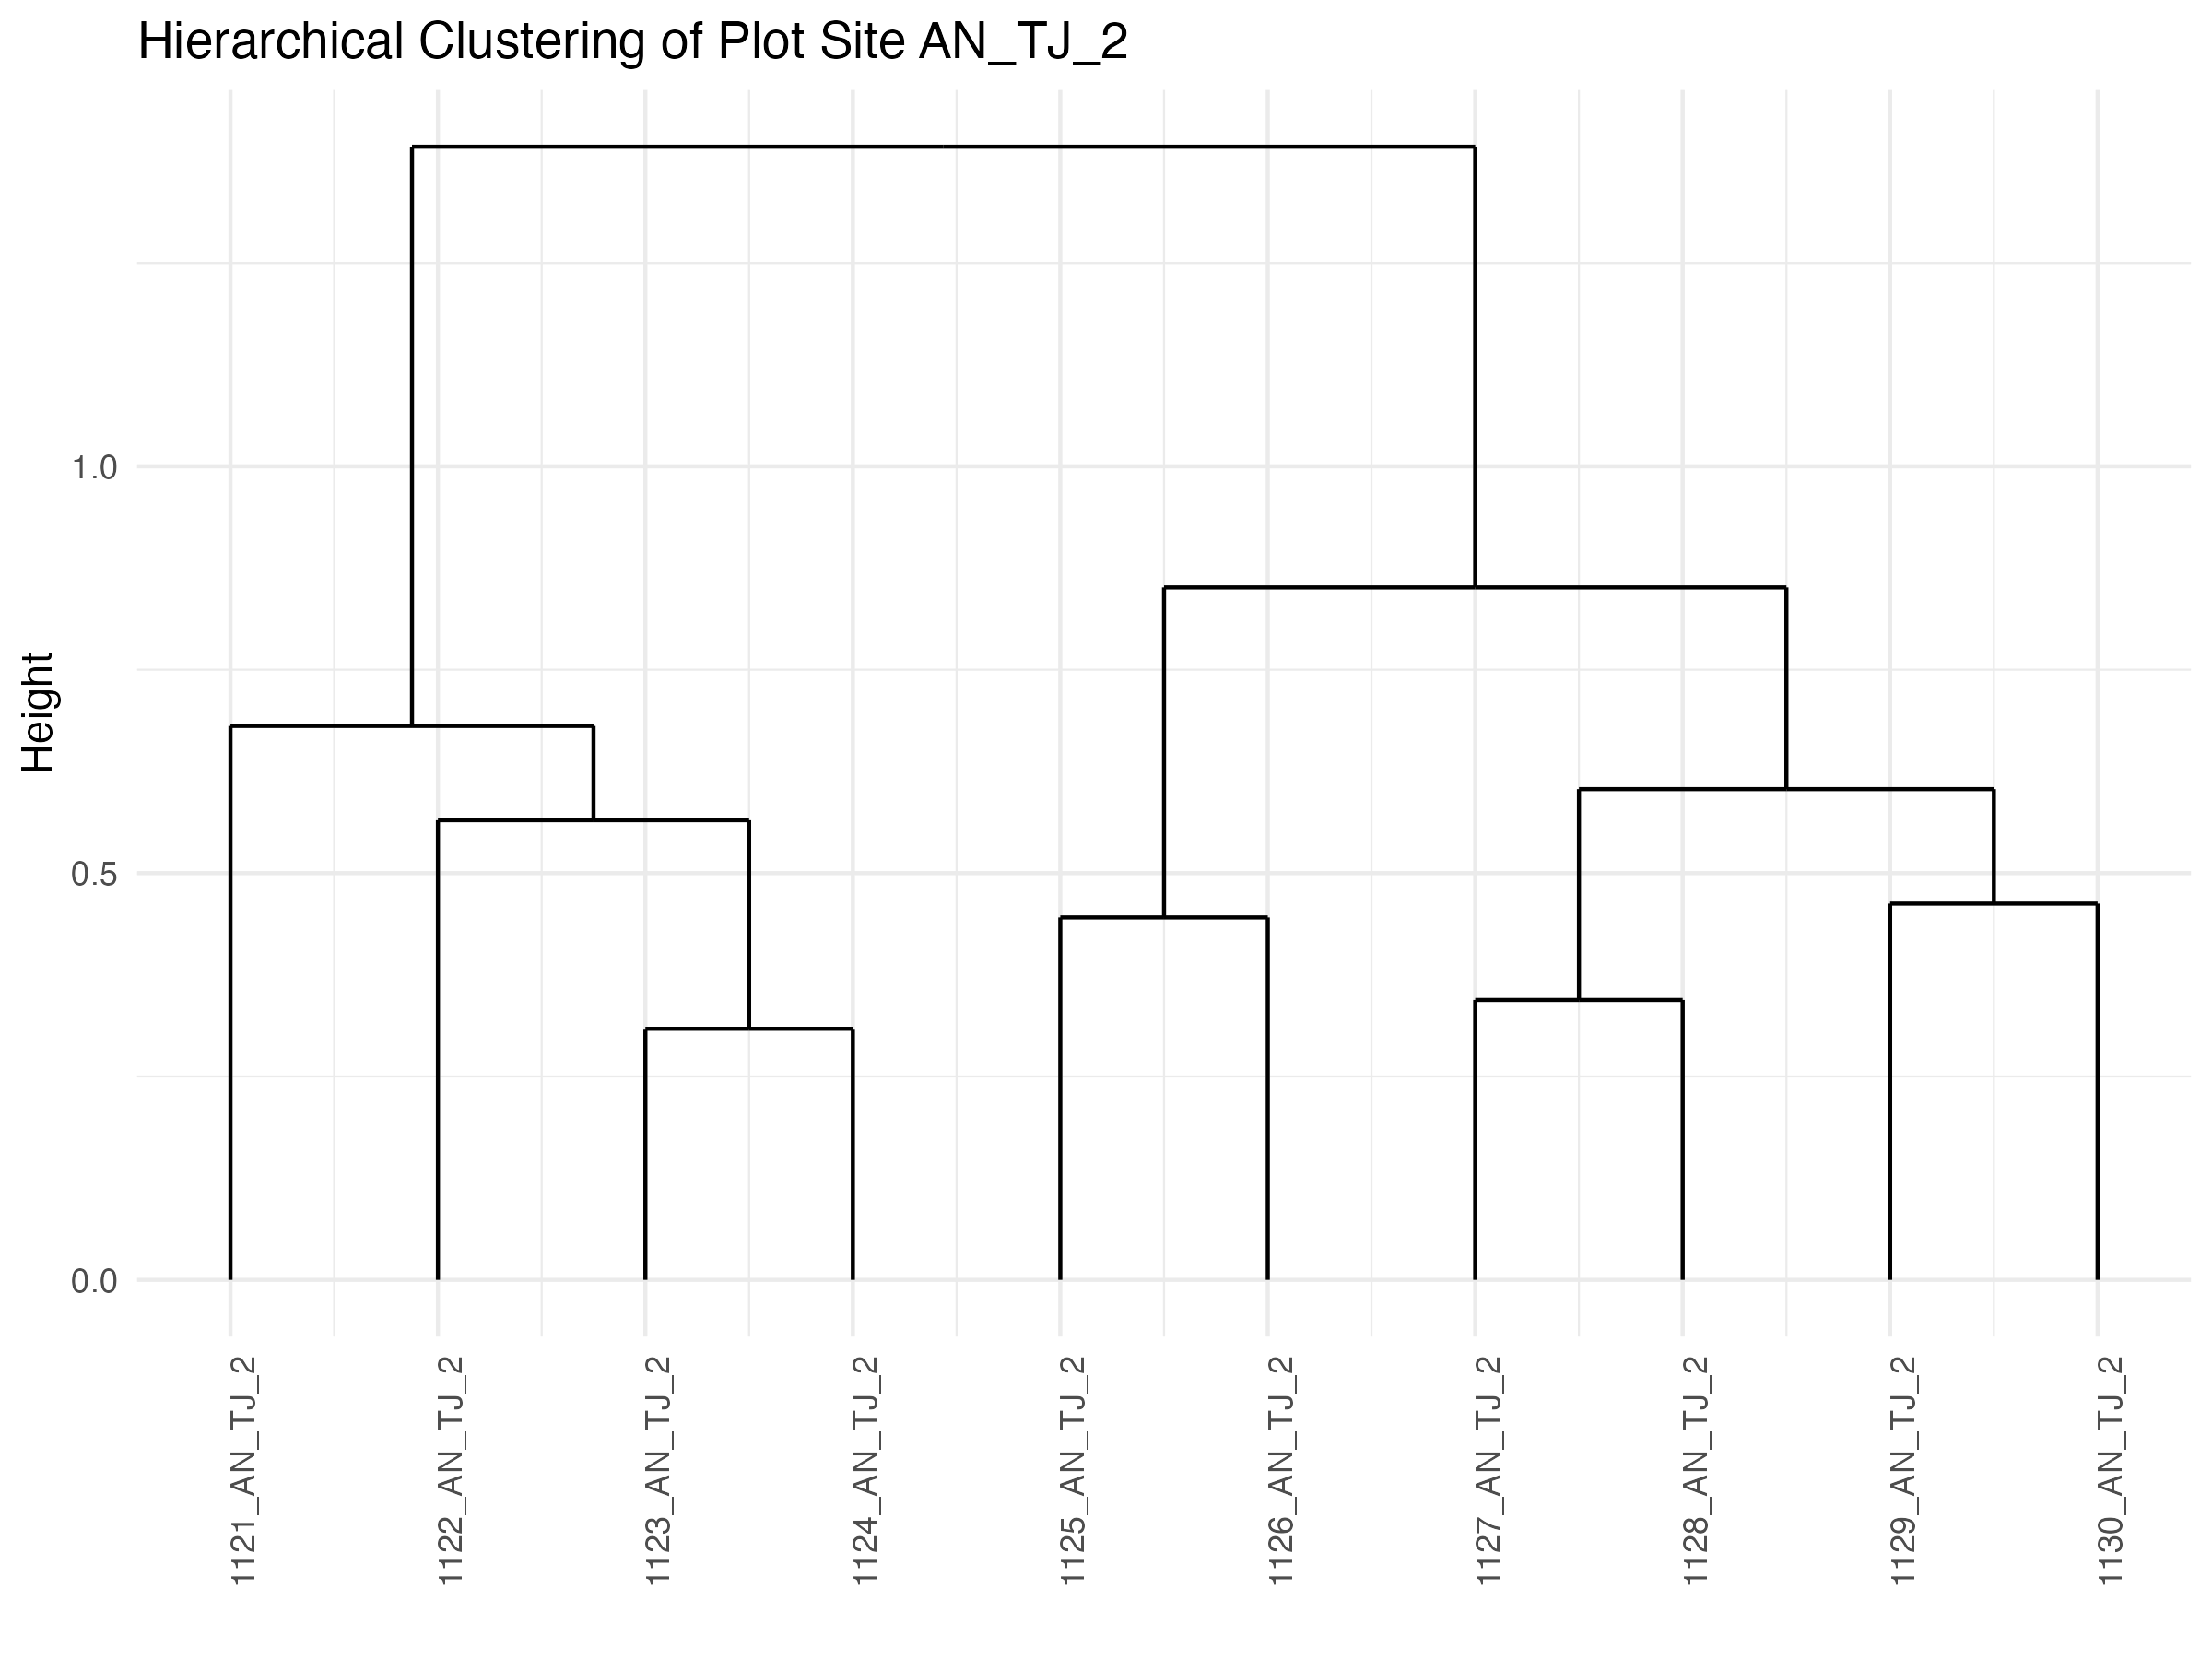
\includegraphics[width=0.9\textwidth]{Figures/Appendix/PlantCommunityClustering/AN_TJ_2_DENDRO.png} % Replace with your actual image path
    \caption{Community cluster dendrogram plot for test site AN\_TJ\_2}
    \label{fig:AN_TJ_2_DENDRO}
\end{figure}

\subsection{ATQ\_VK\_1}
\begin{figure}[H]
    \centering
    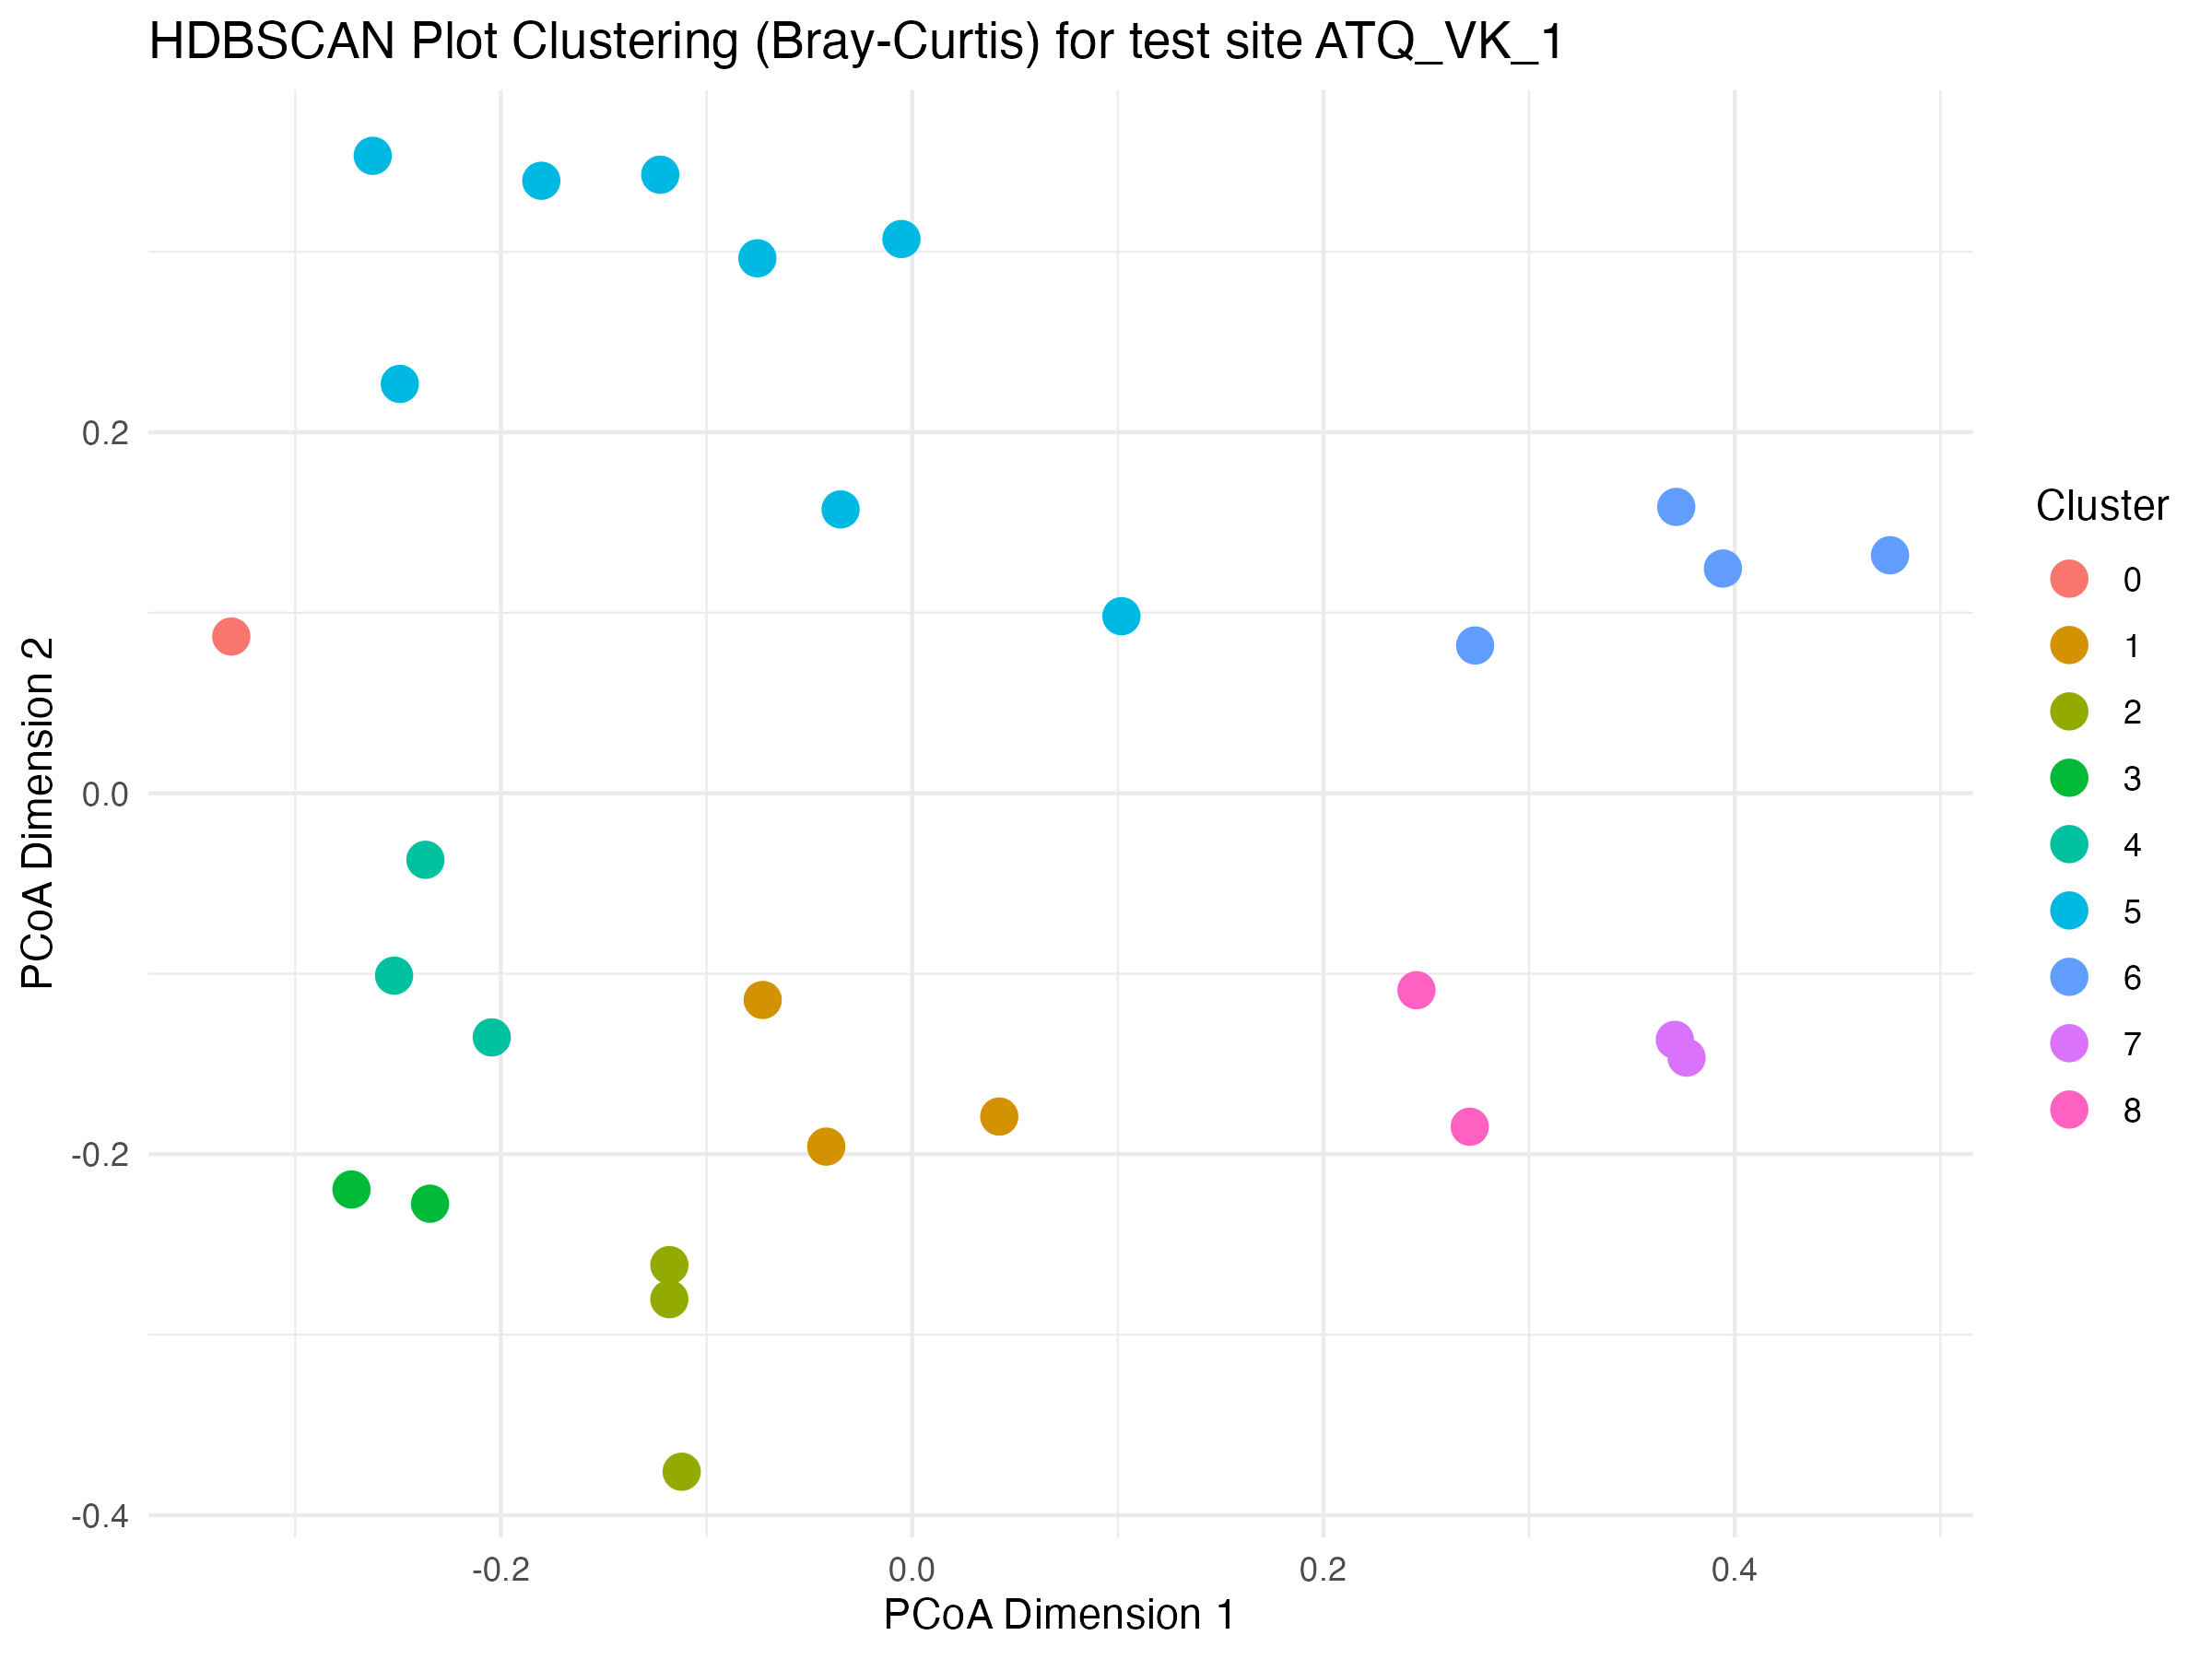
\includegraphics[width=0.9\textwidth]{Figures/Appendix/PlantCommunityClustering/ATQ_VK_1_HDBSCAN_clusters.png} % Replace with your actual image path
    \caption{Community cluster HDBSCAN plot for test site ATQ\_VK\_1}
    \label{fig:ATQ_VK_1_HDBSCAN_clusters}
\end{figure}

\begin{figure}[H]
    \centering
    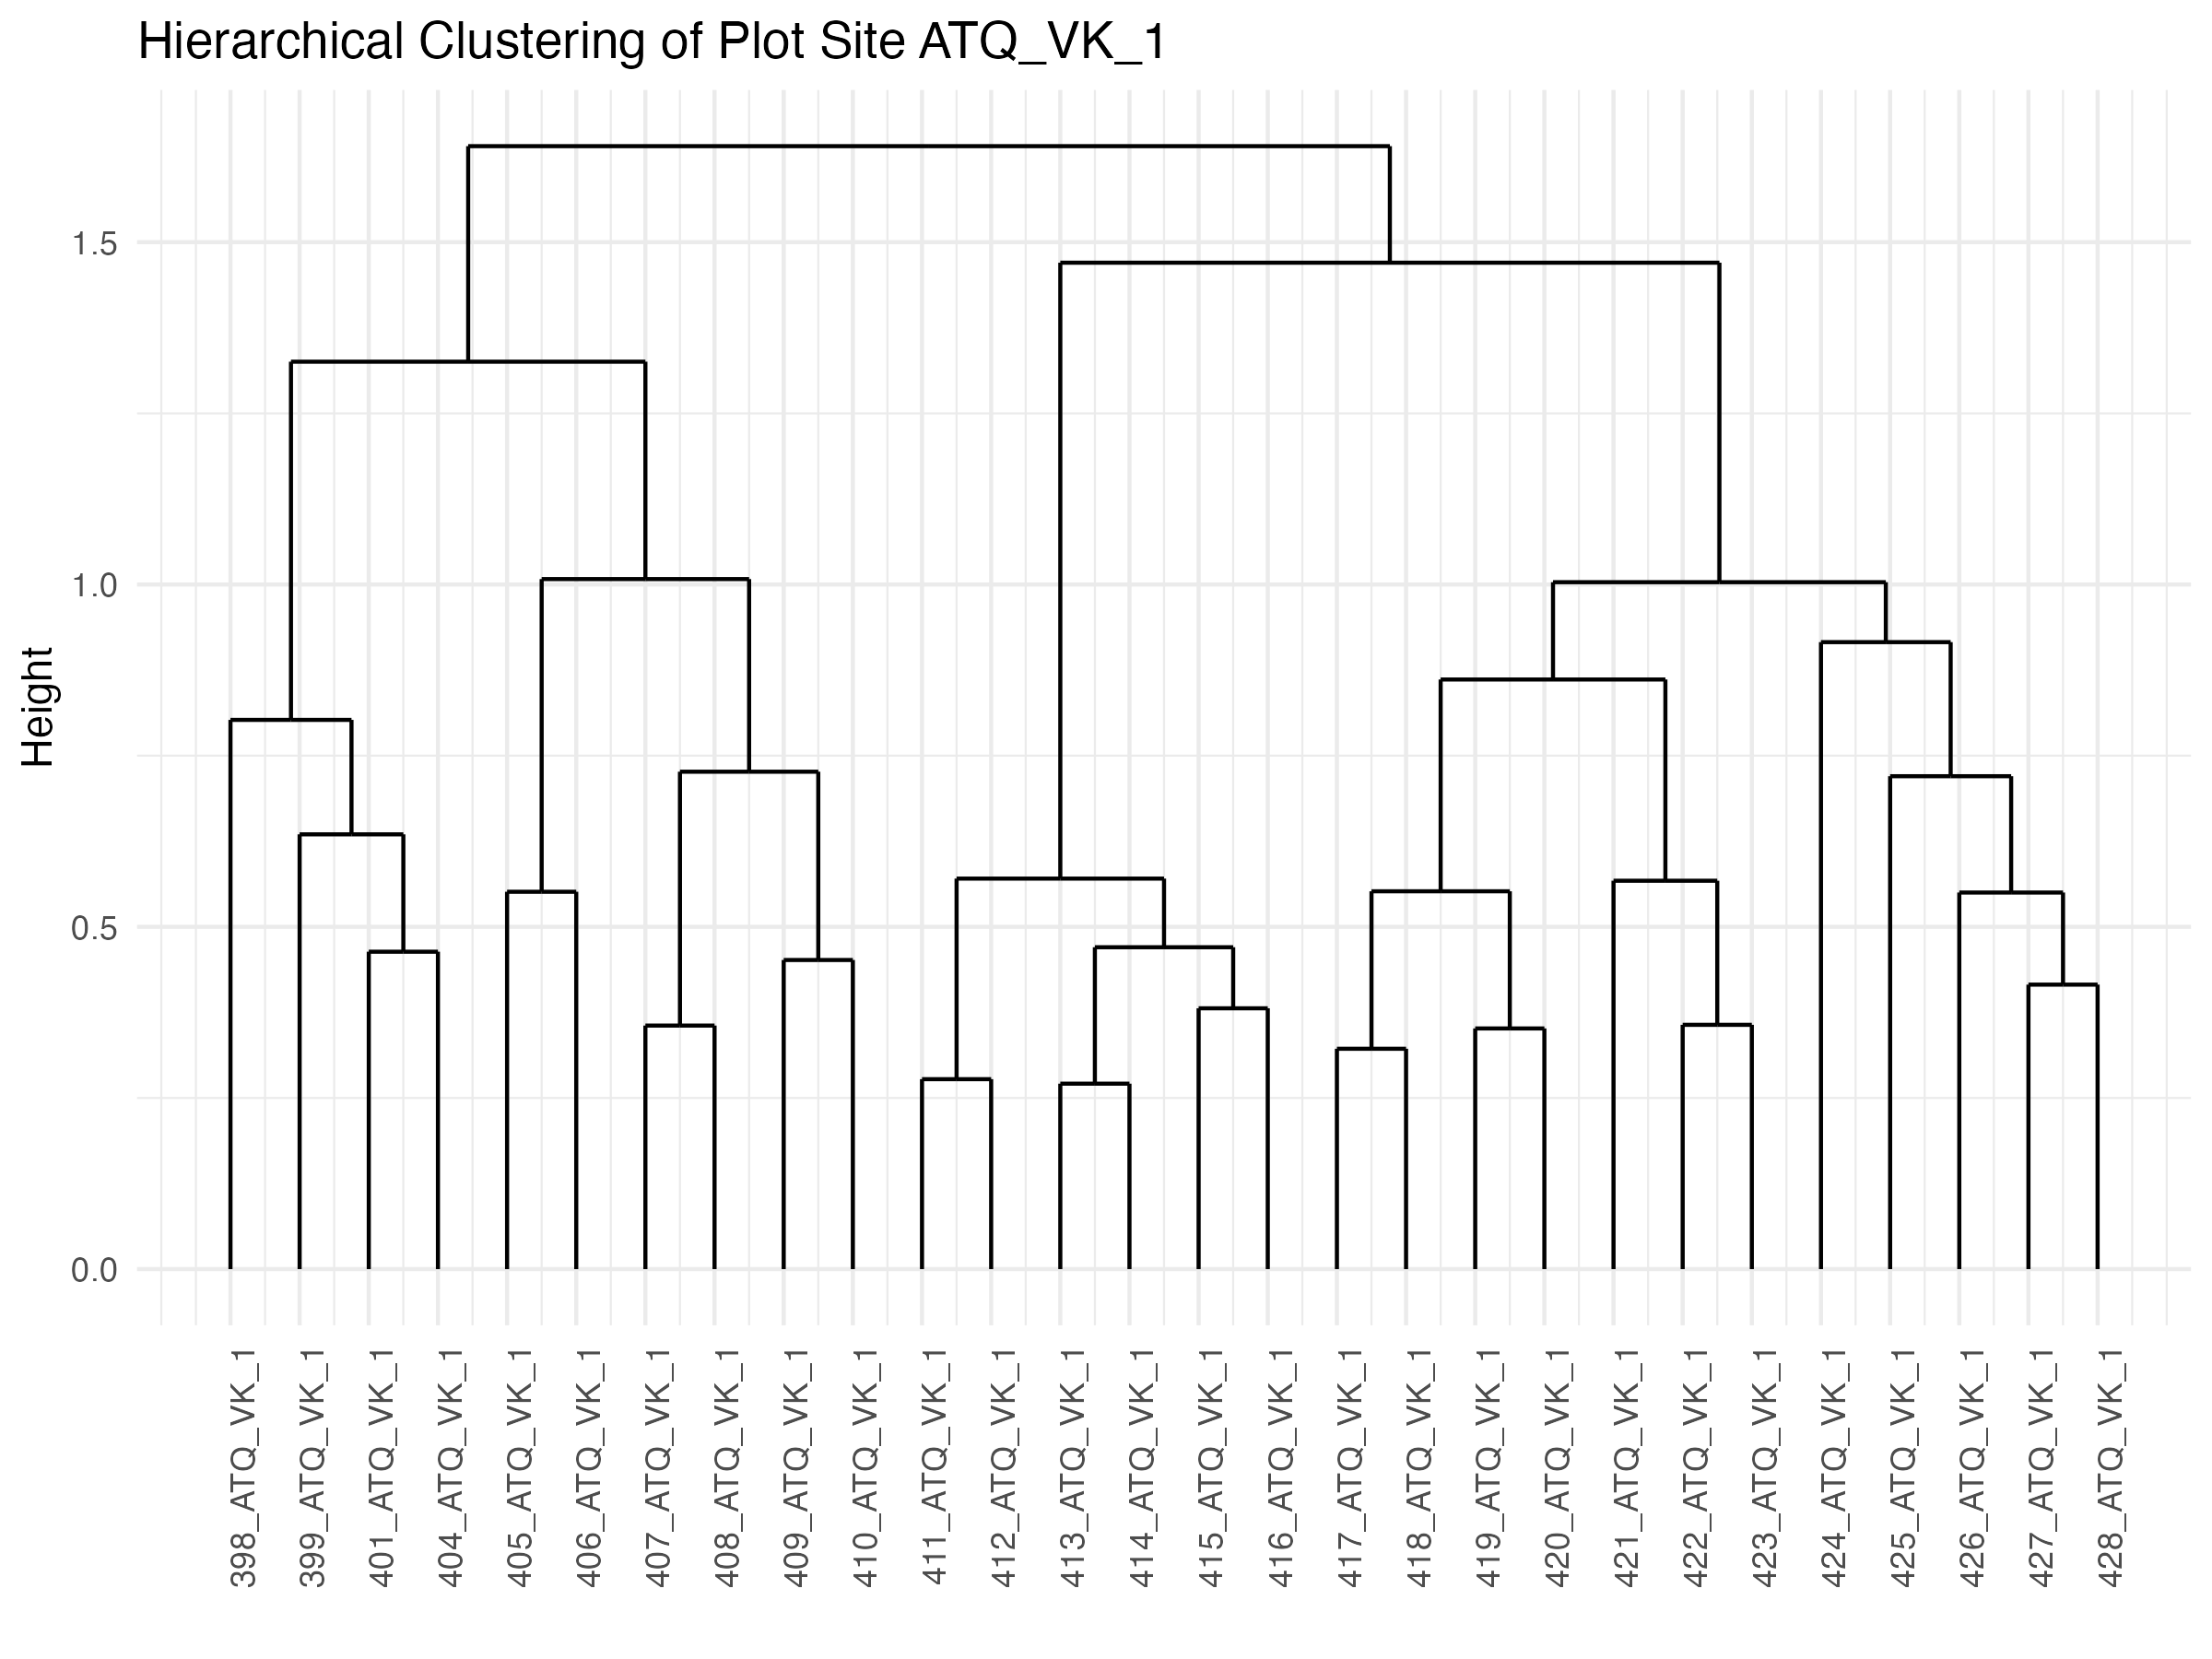
\includegraphics[width=0.9\textwidth]{Figures/Appendix/PlantCommunityClustering/ATQ_VK_1_DENDRO.png} % Replace with your actual image path
    \caption{Community cluster dendrogram plot for test site ATQ\_VK\_1}
    \label{fig:ATQ_VK_1_DENDRO}
\end{figure}

\subsection{BRW\_PW\_1}
\begin{figure}[H]
    \centering
    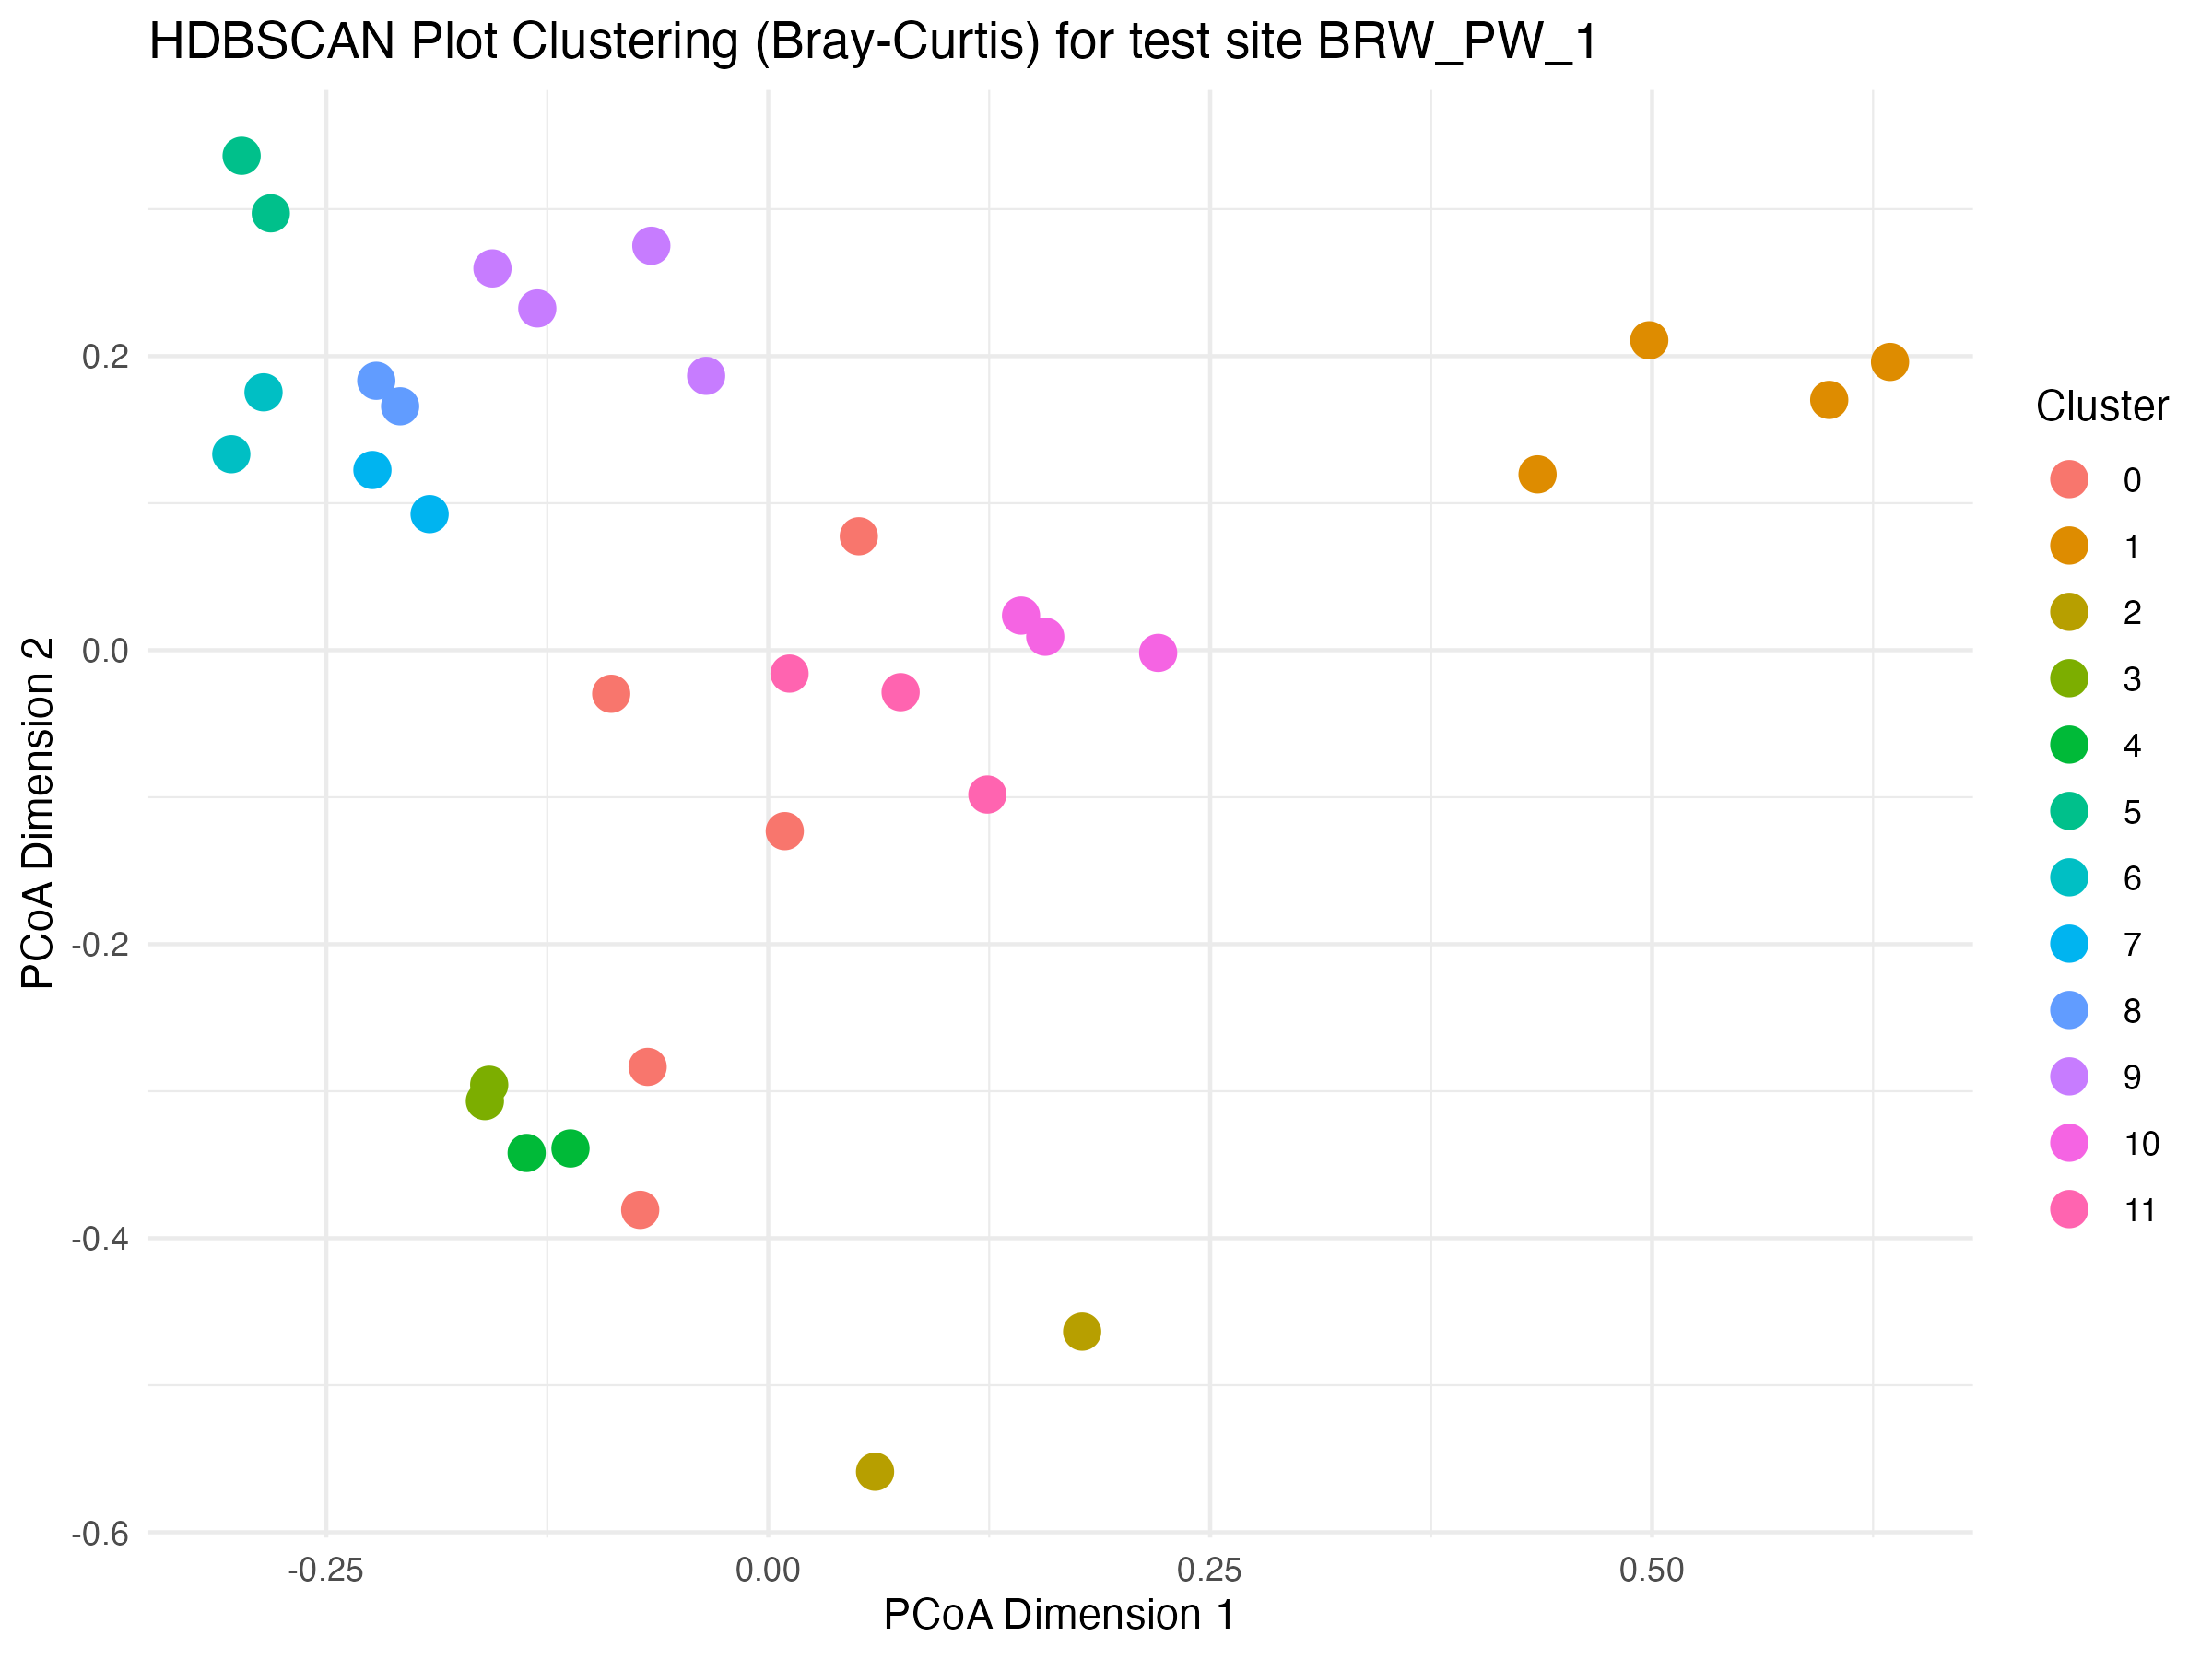
\includegraphics[width=0.9\textwidth]{Figures/Appendix/PlantCommunityClustering/BRW_PW_1_HDBSCAN_clusters.png} % Replace with your actual image path
    \caption{Community cluster HDBSCAN plot for test site BRW\_PW\_1}
    \label{fig:BRW_PW_1_HDBSCAN_clusters}
\end{figure}

\begin{figure}[H]
    \centering
    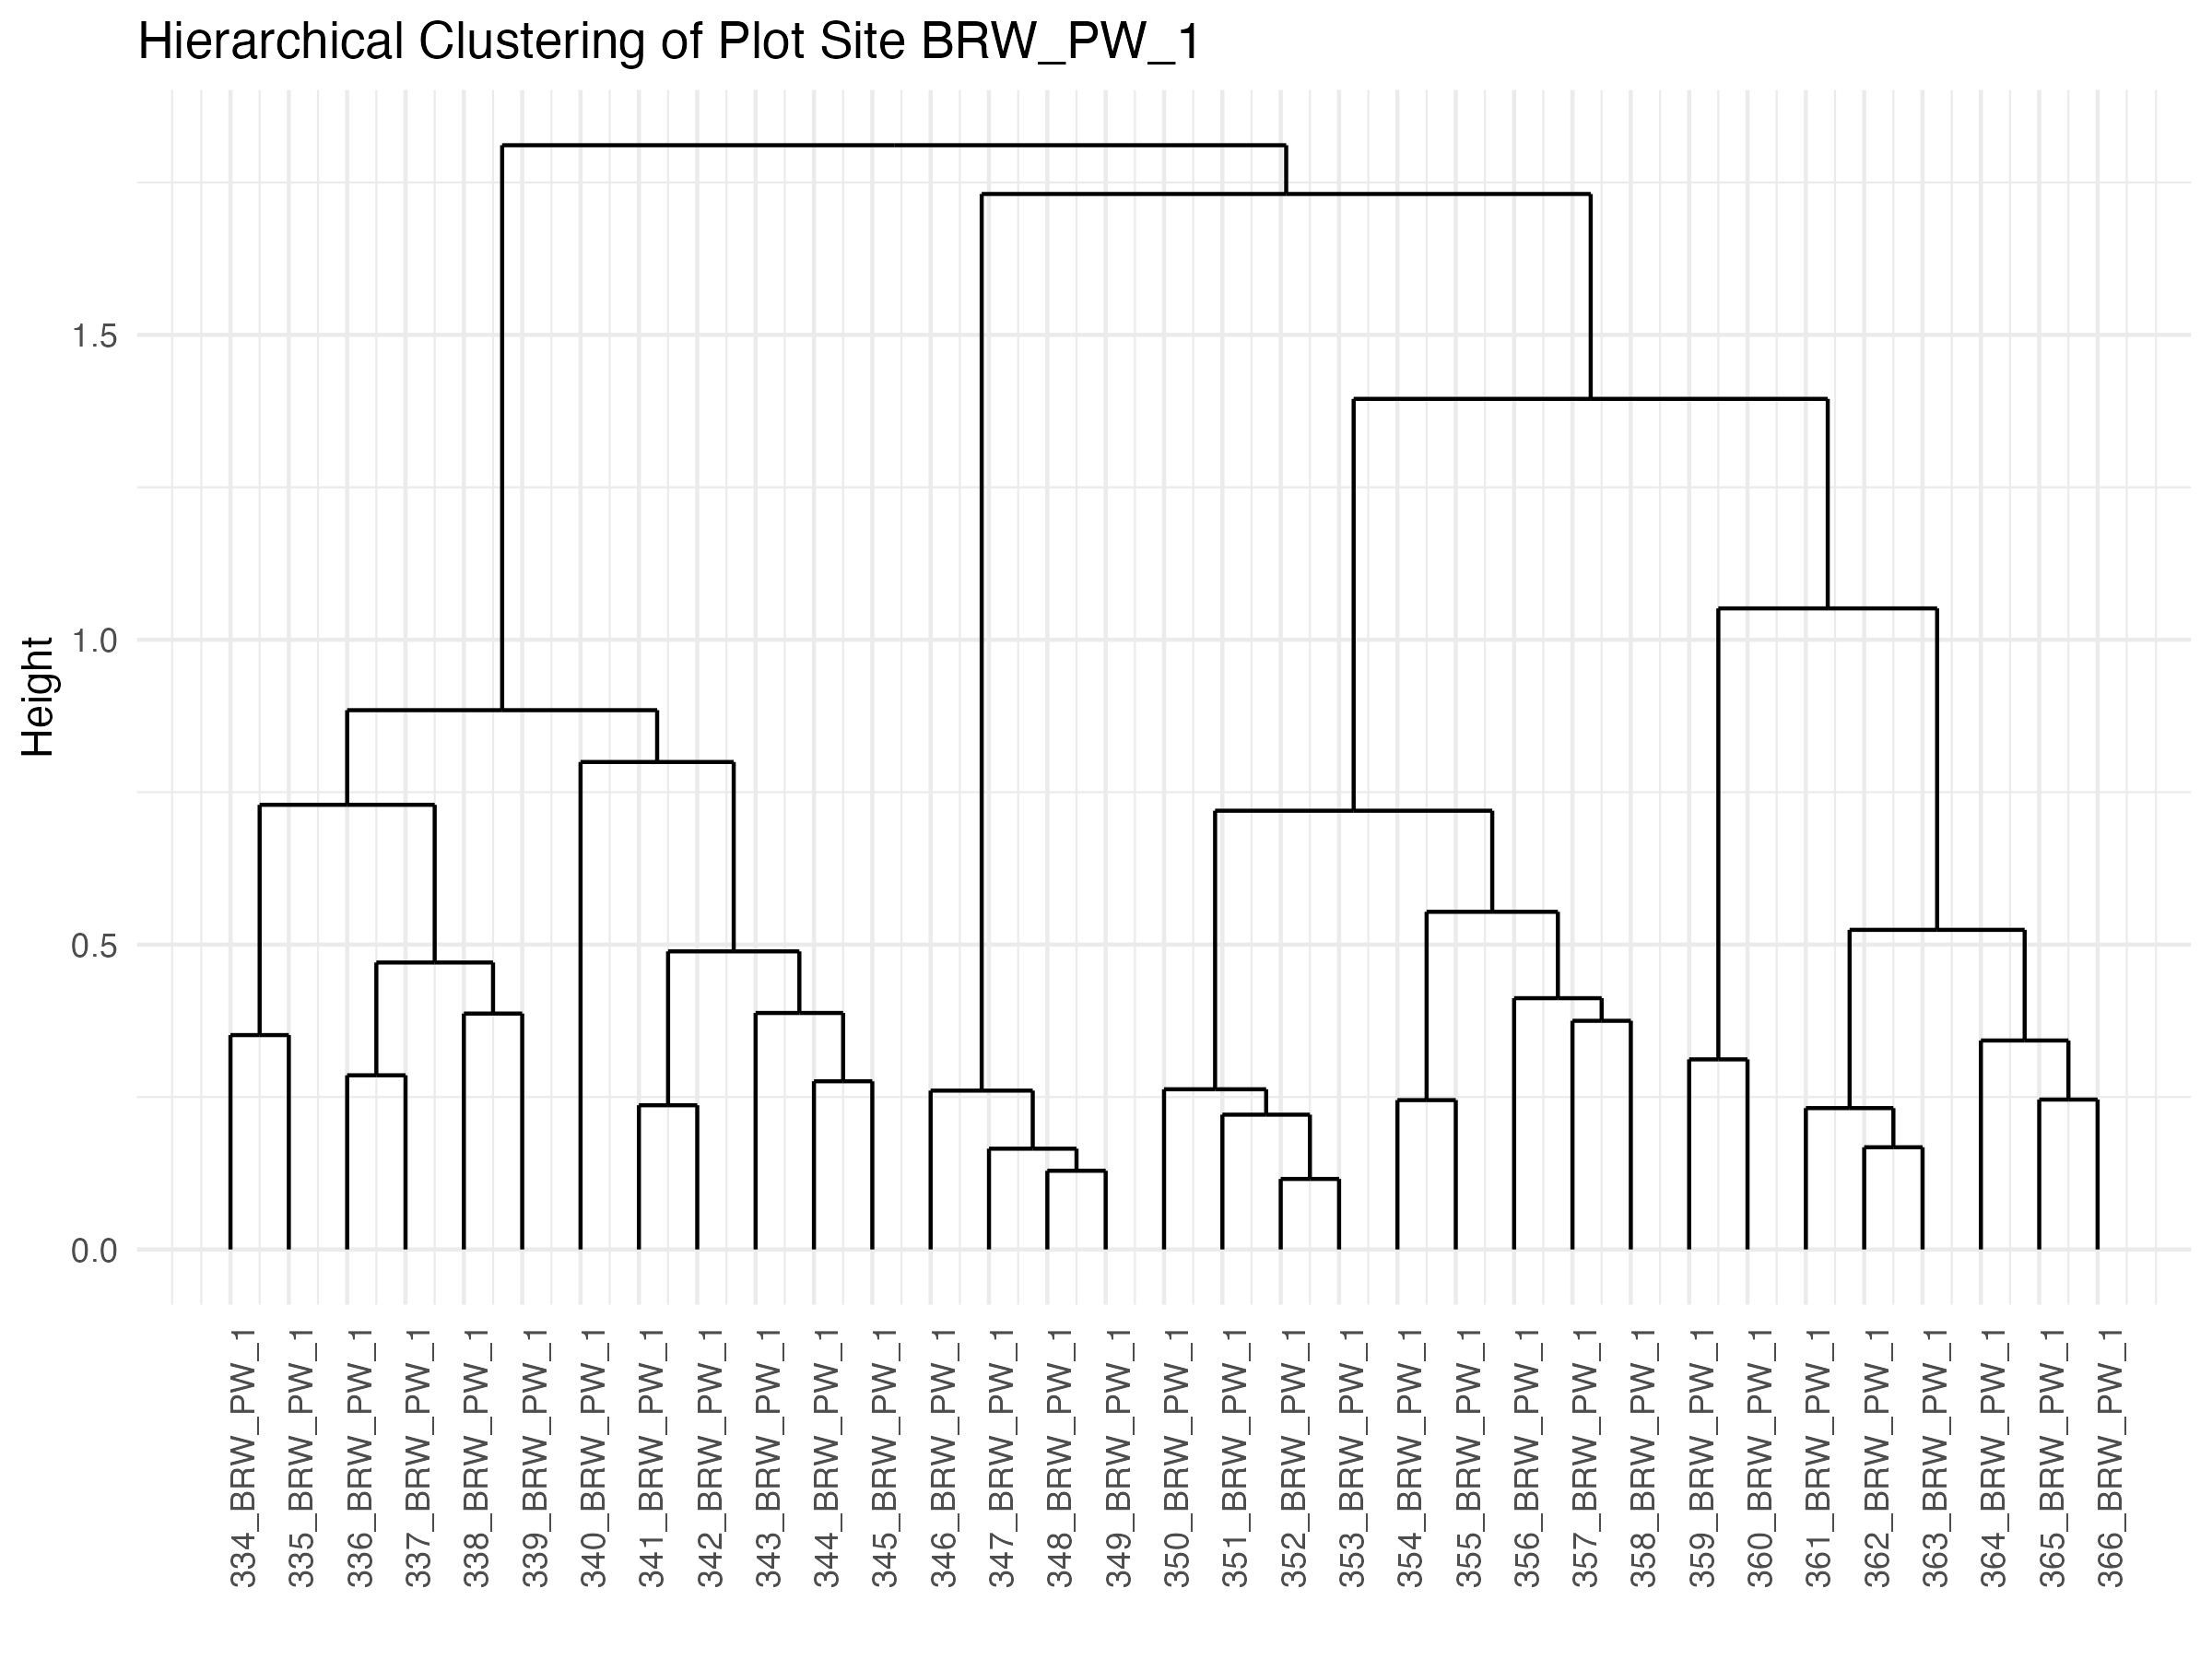
\includegraphics[width=0.9\textwidth]{Figures/Appendix/PlantCommunityClustering/BRW_PW_1_DENDRO.png} % Replace with your actual image path
    \caption{Community cluster dendrogram plot for test site BRW\_PW\_1}
    \label{fig:BRW_PW_1_DENDRO}
\end{figure}

\subsection{BRW\_VS\_1}
\begin{figure}[H]
    \centering
    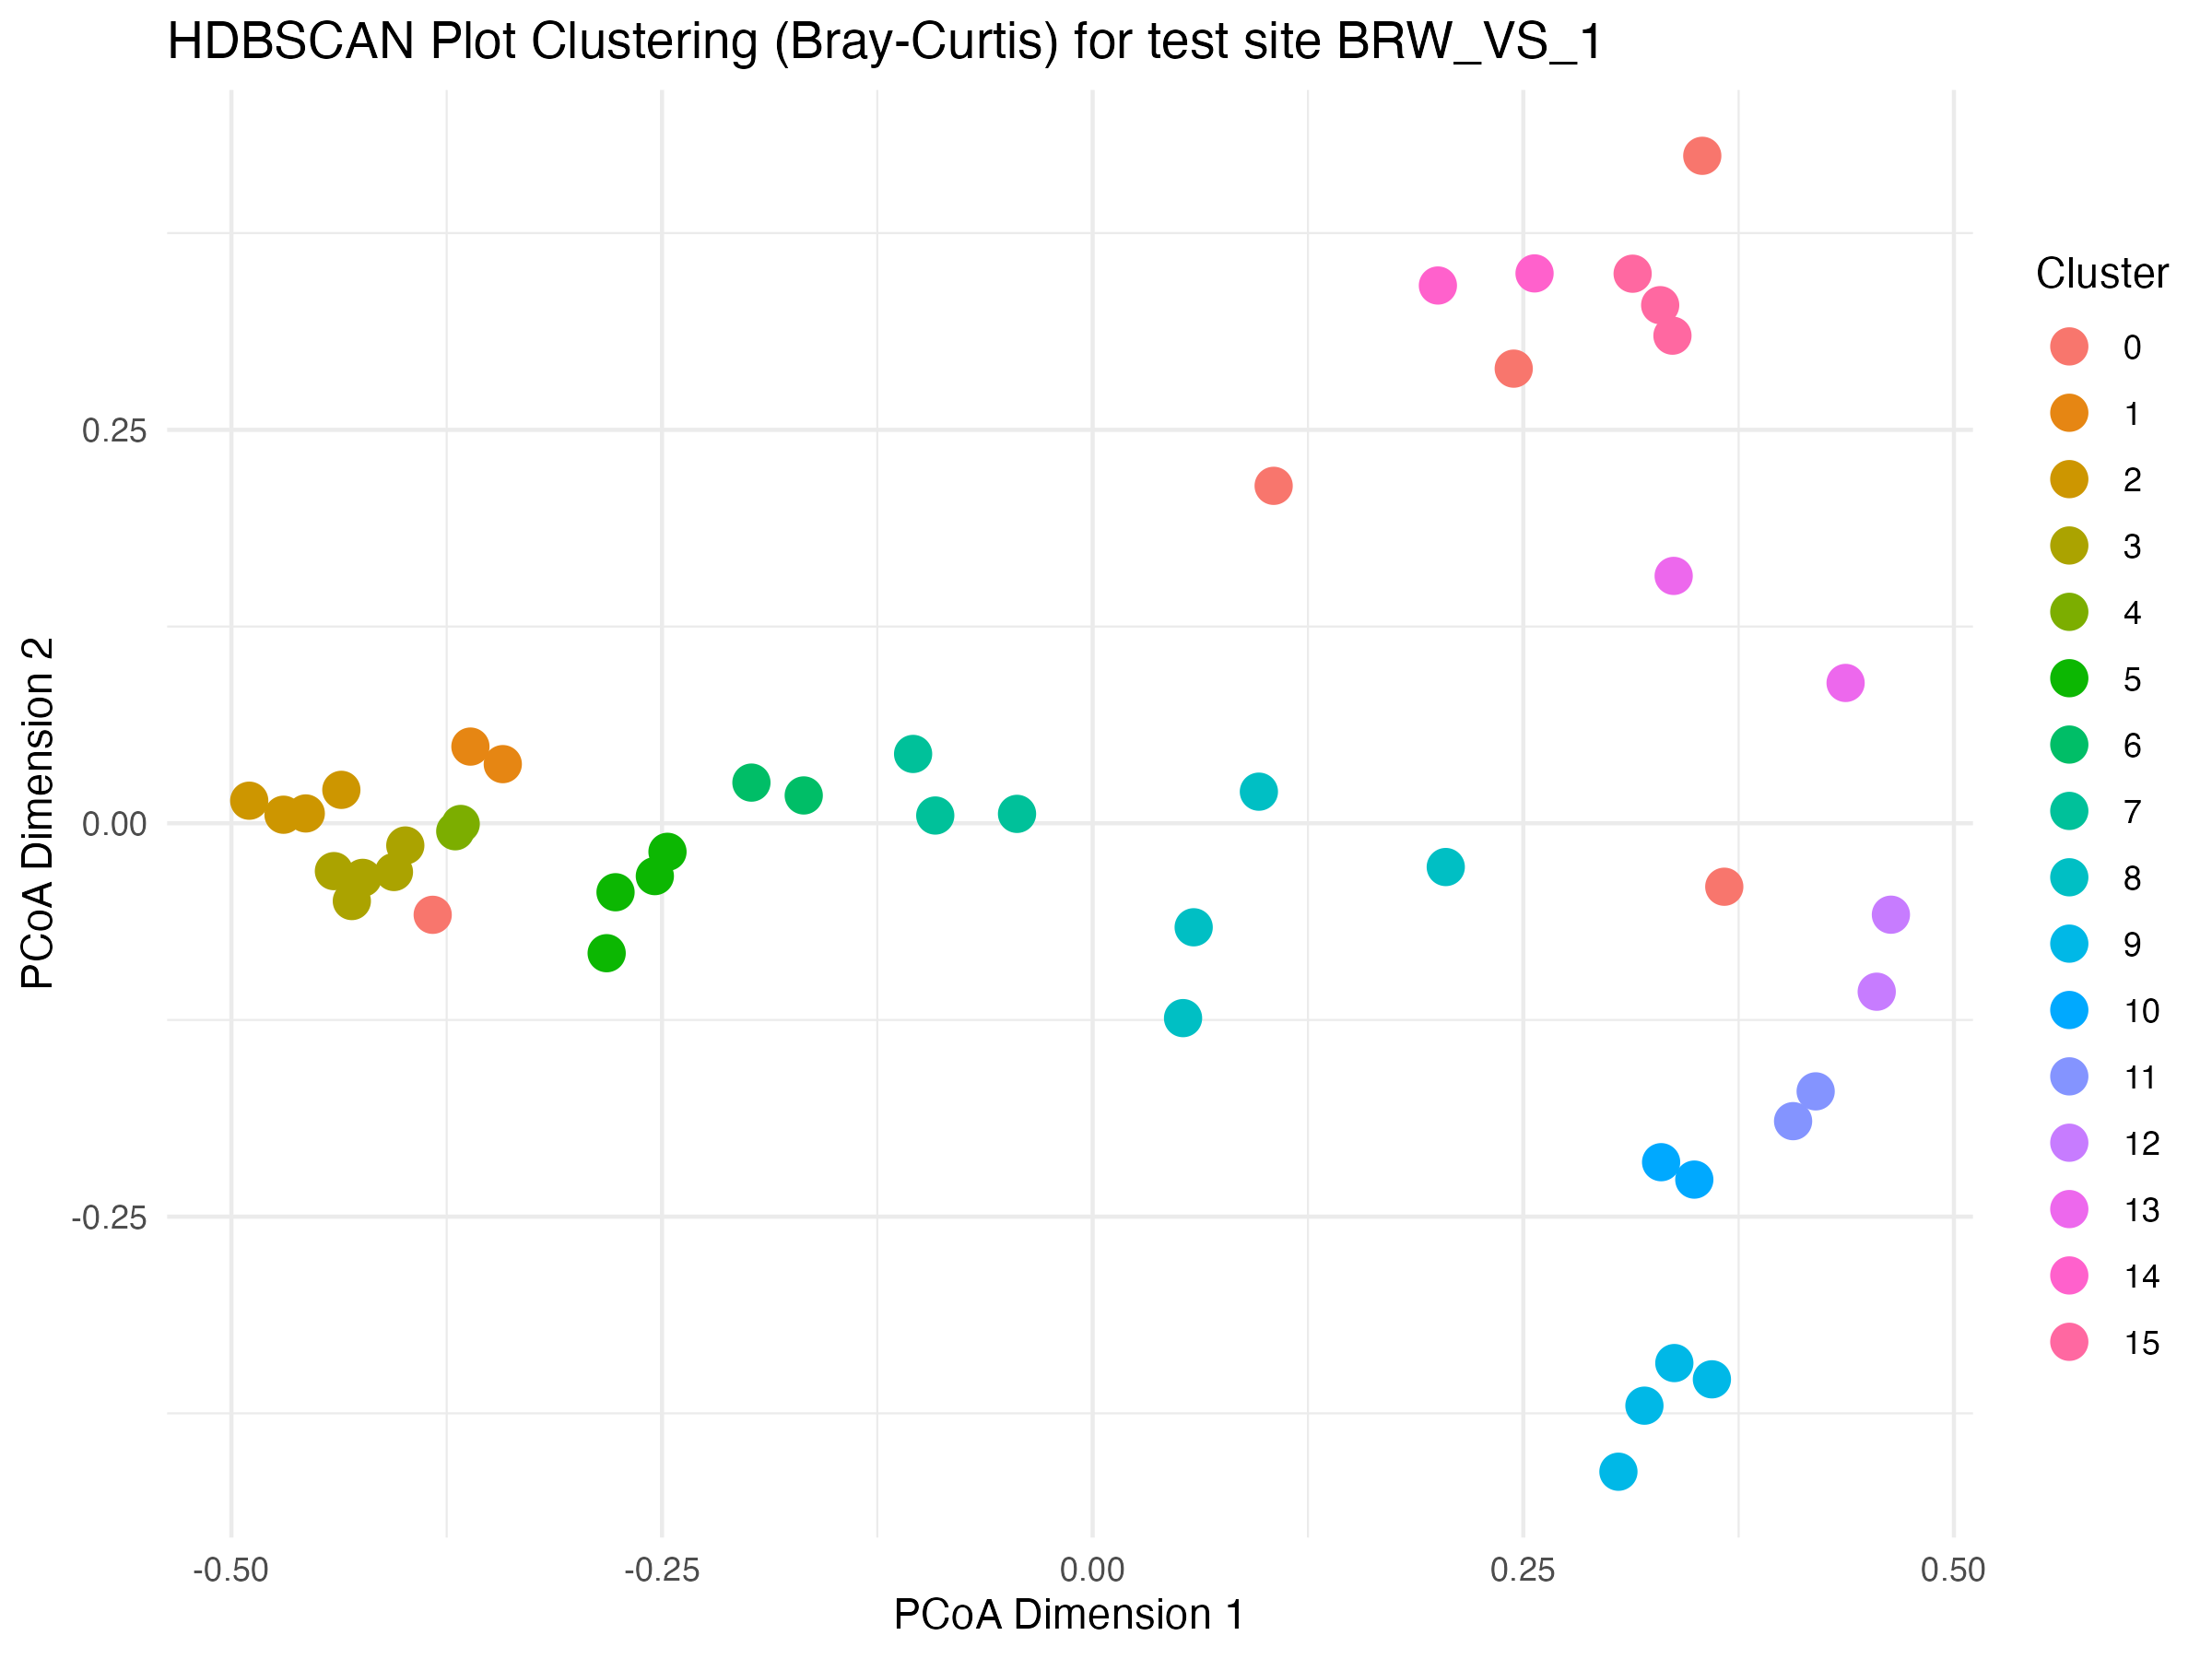
\includegraphics[width=0.9\textwidth]{Figures/Appendix/PlantCommunityClustering/BRW_VS_1_HDBSCAN_clusters.png} % Replace with your actual image path
    \caption{Community cluster HDBSCAN plot for test site BRW\_VS\_1}
    \label{fig:BRW_VS_1_HDBSCAN_clusters}
\end{figure}

\begin{figure}[H]
    \centering
    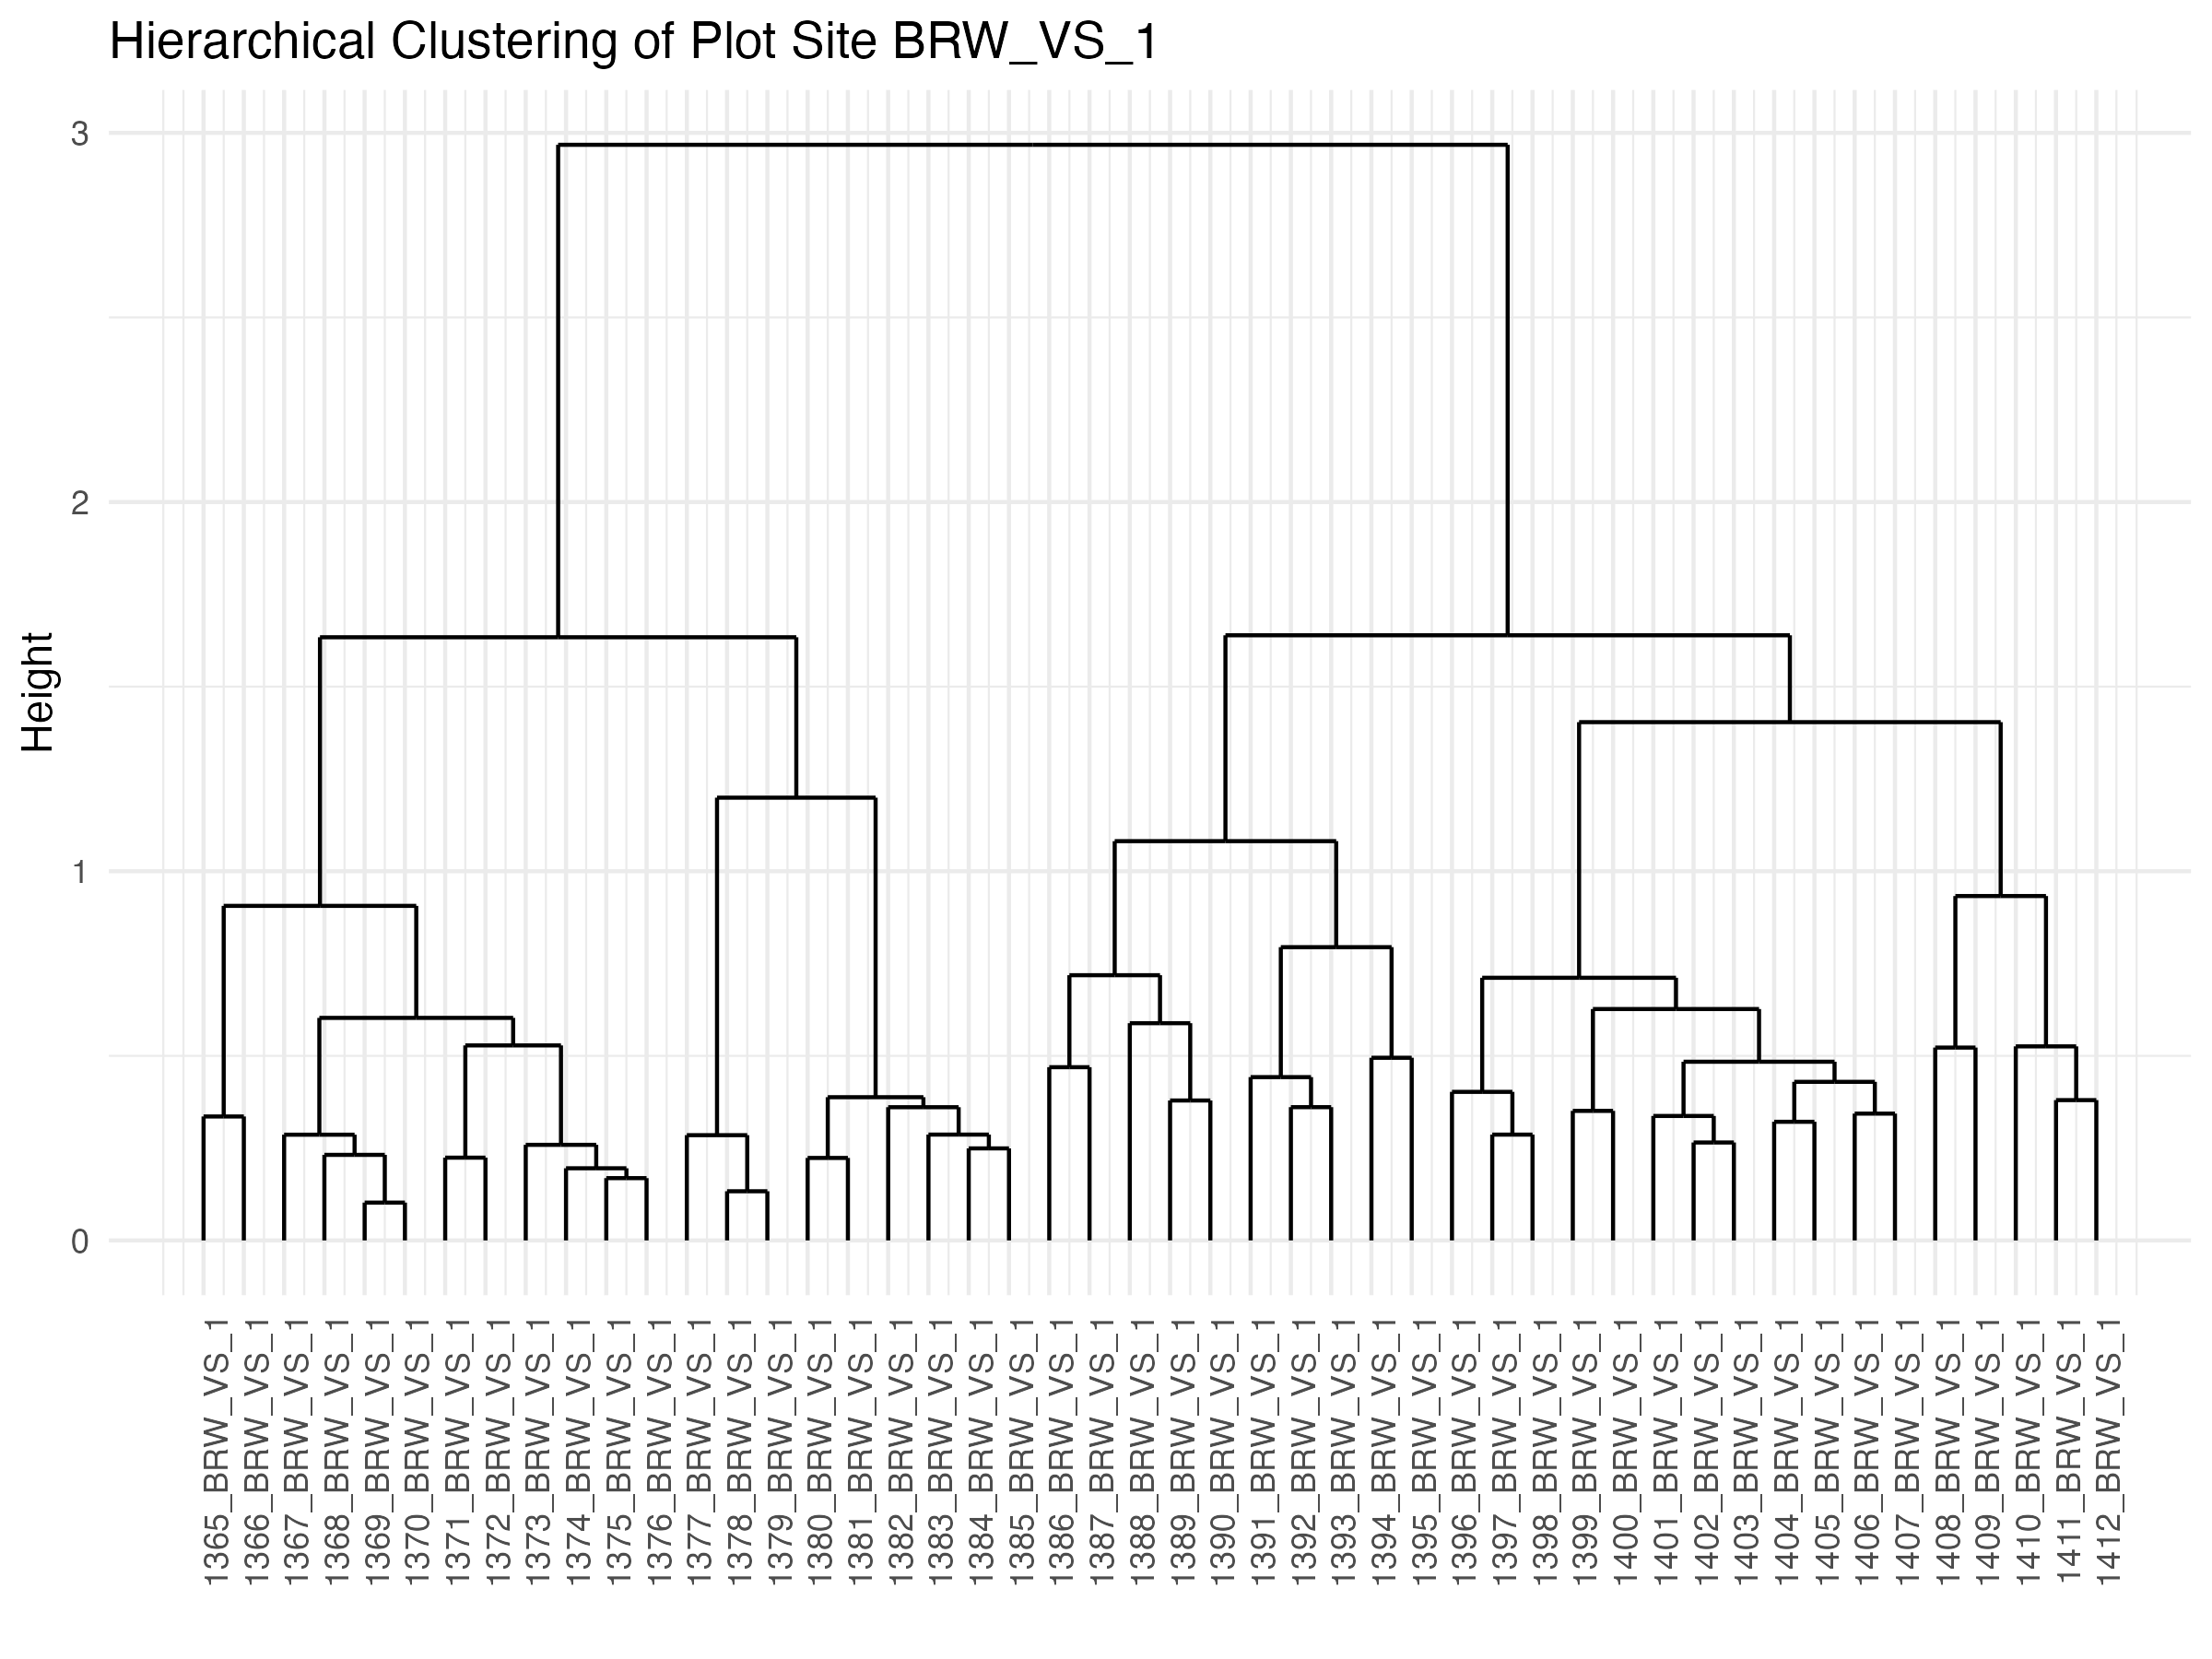
\includegraphics[width=0.9\textwidth]{Figures/Appendix/PlantCommunityClustering/BRW_VS_1_DENDRO.png} % Replace with your actual image path
    \caption{Community cluster dendrogram plot for test site BRW\_VS\_1}
    \label{fig:BRW_VS_1_DENDRO}
\end{figure}

\subsection{FLXTWRZONA\_SD\_1}
\begin{figure}[H]
    \centering
    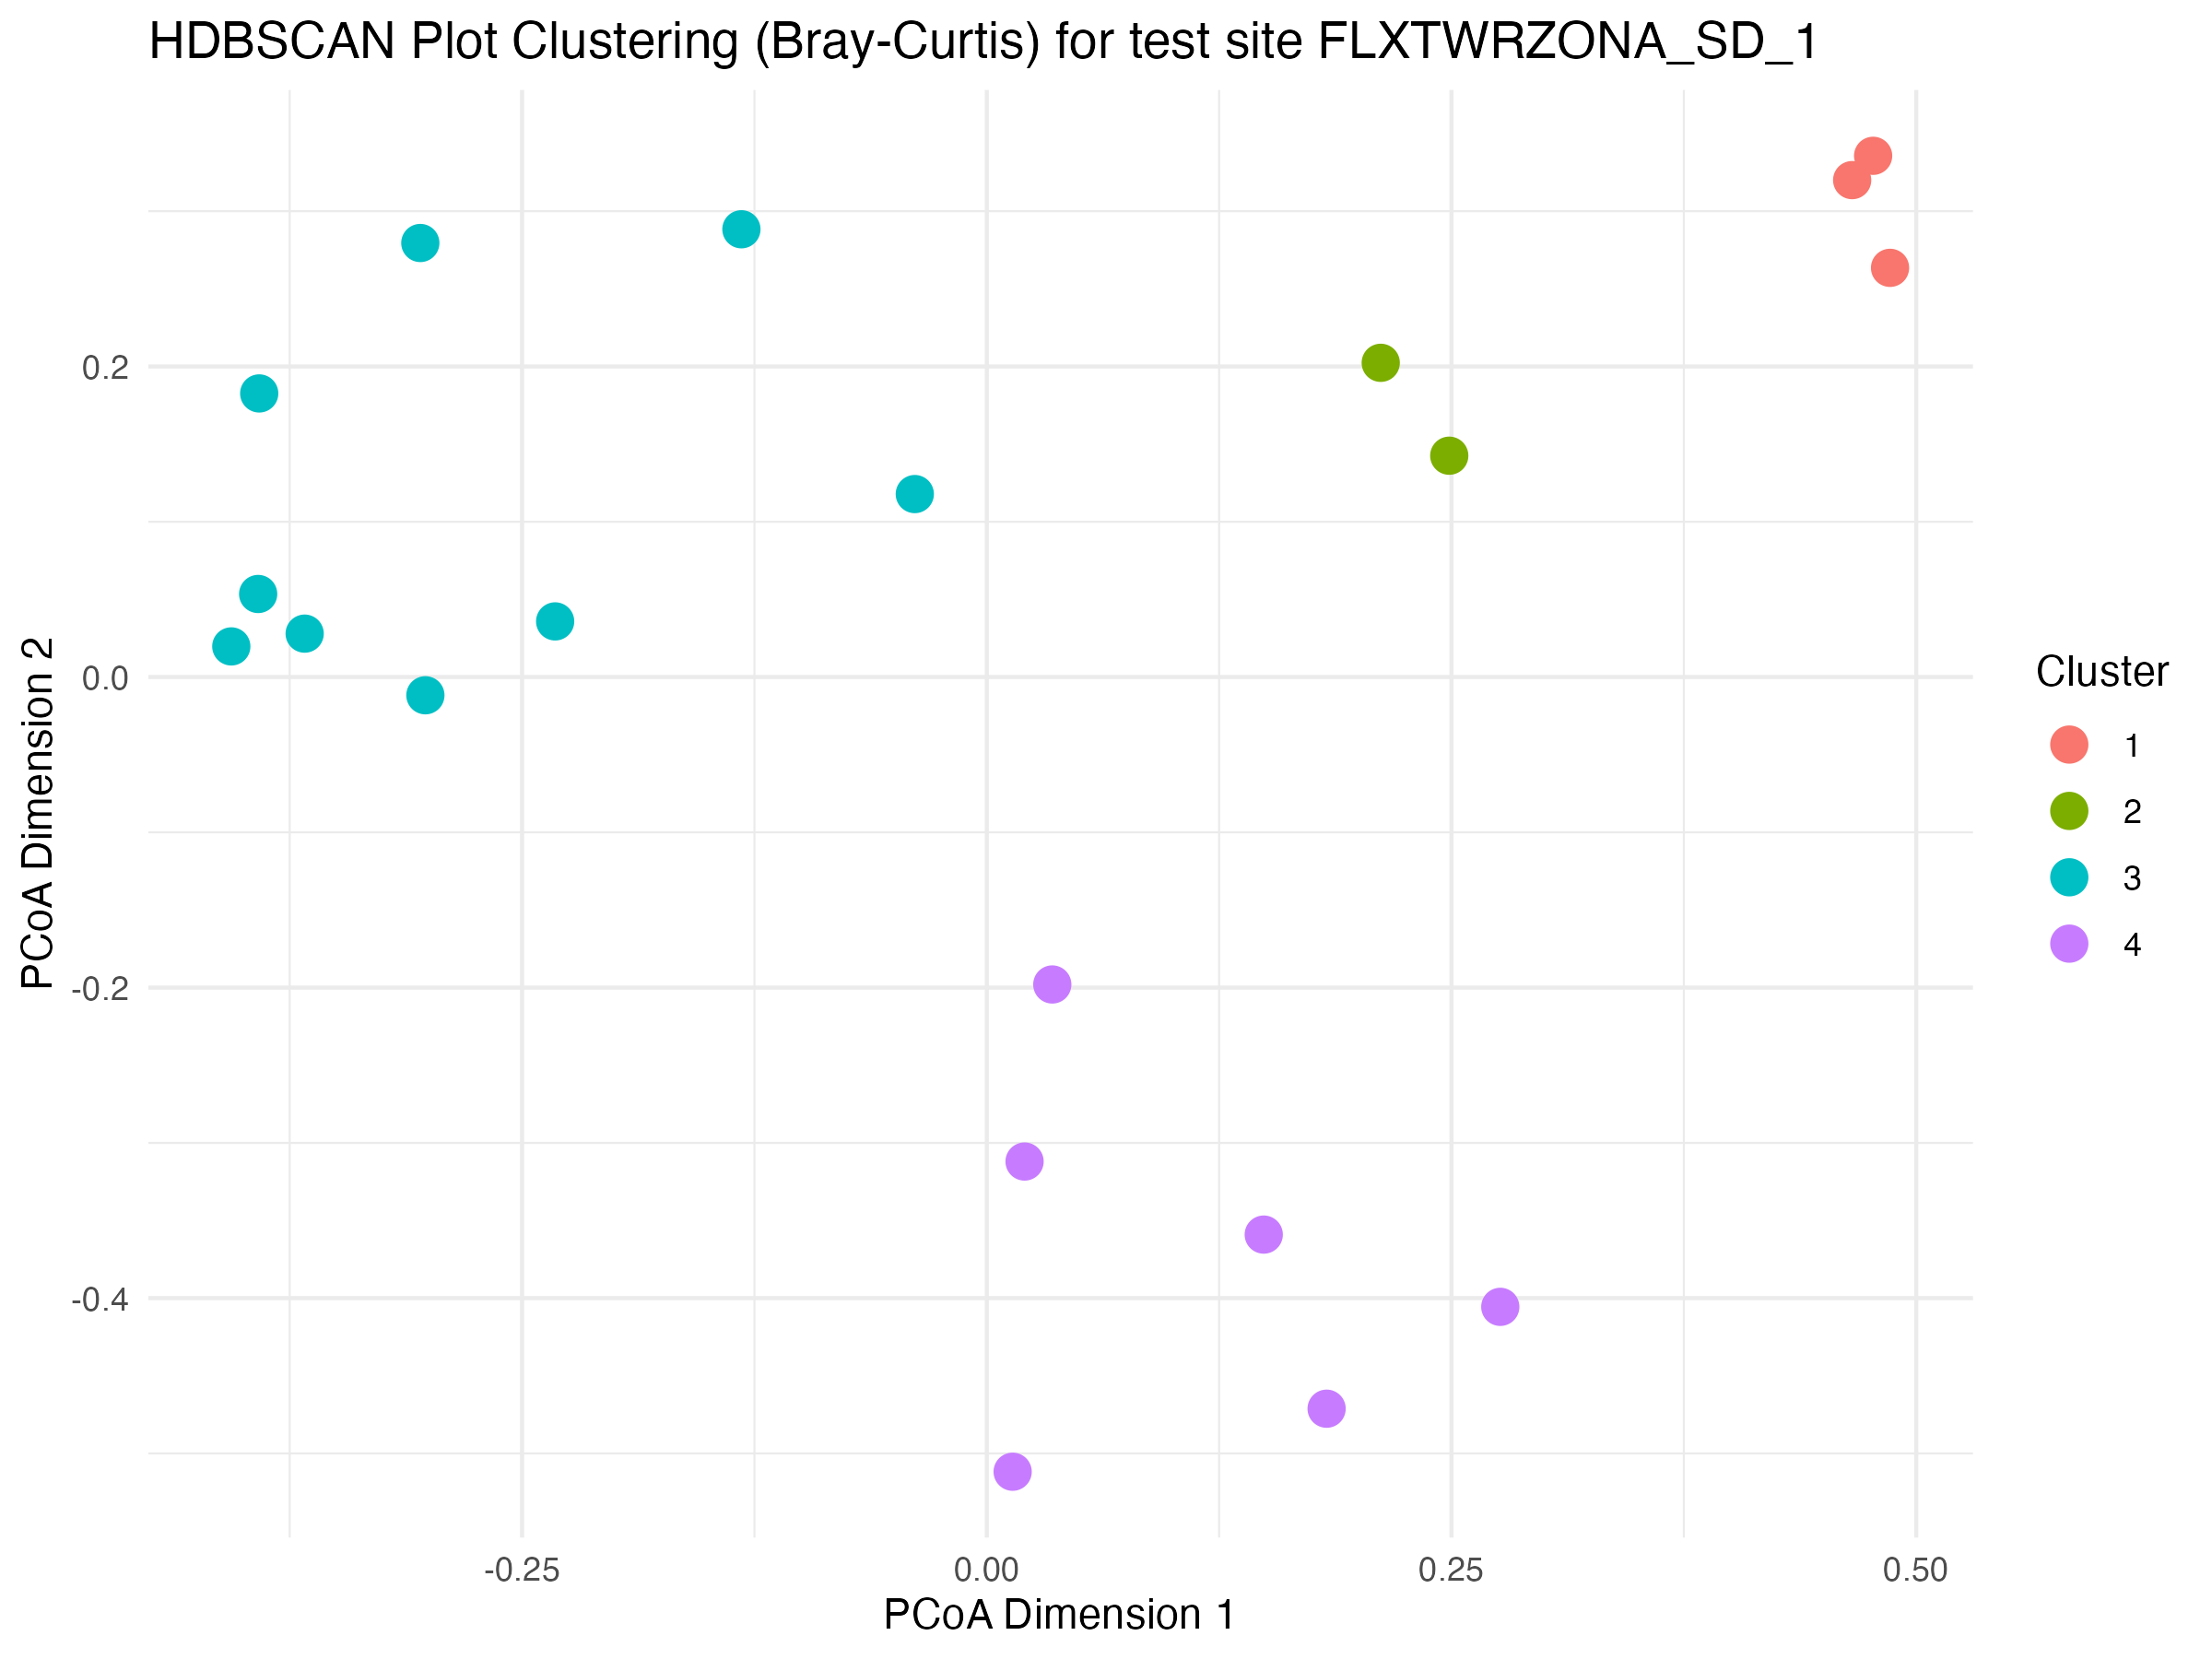
\includegraphics[width=0.9\textwidth]{Figures/Appendix/PlantCommunityClustering/FLXTWRZONA_SD_1_HDBSCAN_clusters.png} % Replace with your actual image path
    \caption{Community cluster HDBSCAN plot for test site FLXTWRZONA\_SD\_1}
    \label{fig:FLXTWRZONA_SD_1_HDBSCAN_clusters}
\end{figure}

\begin{figure}[H]
    \centering
    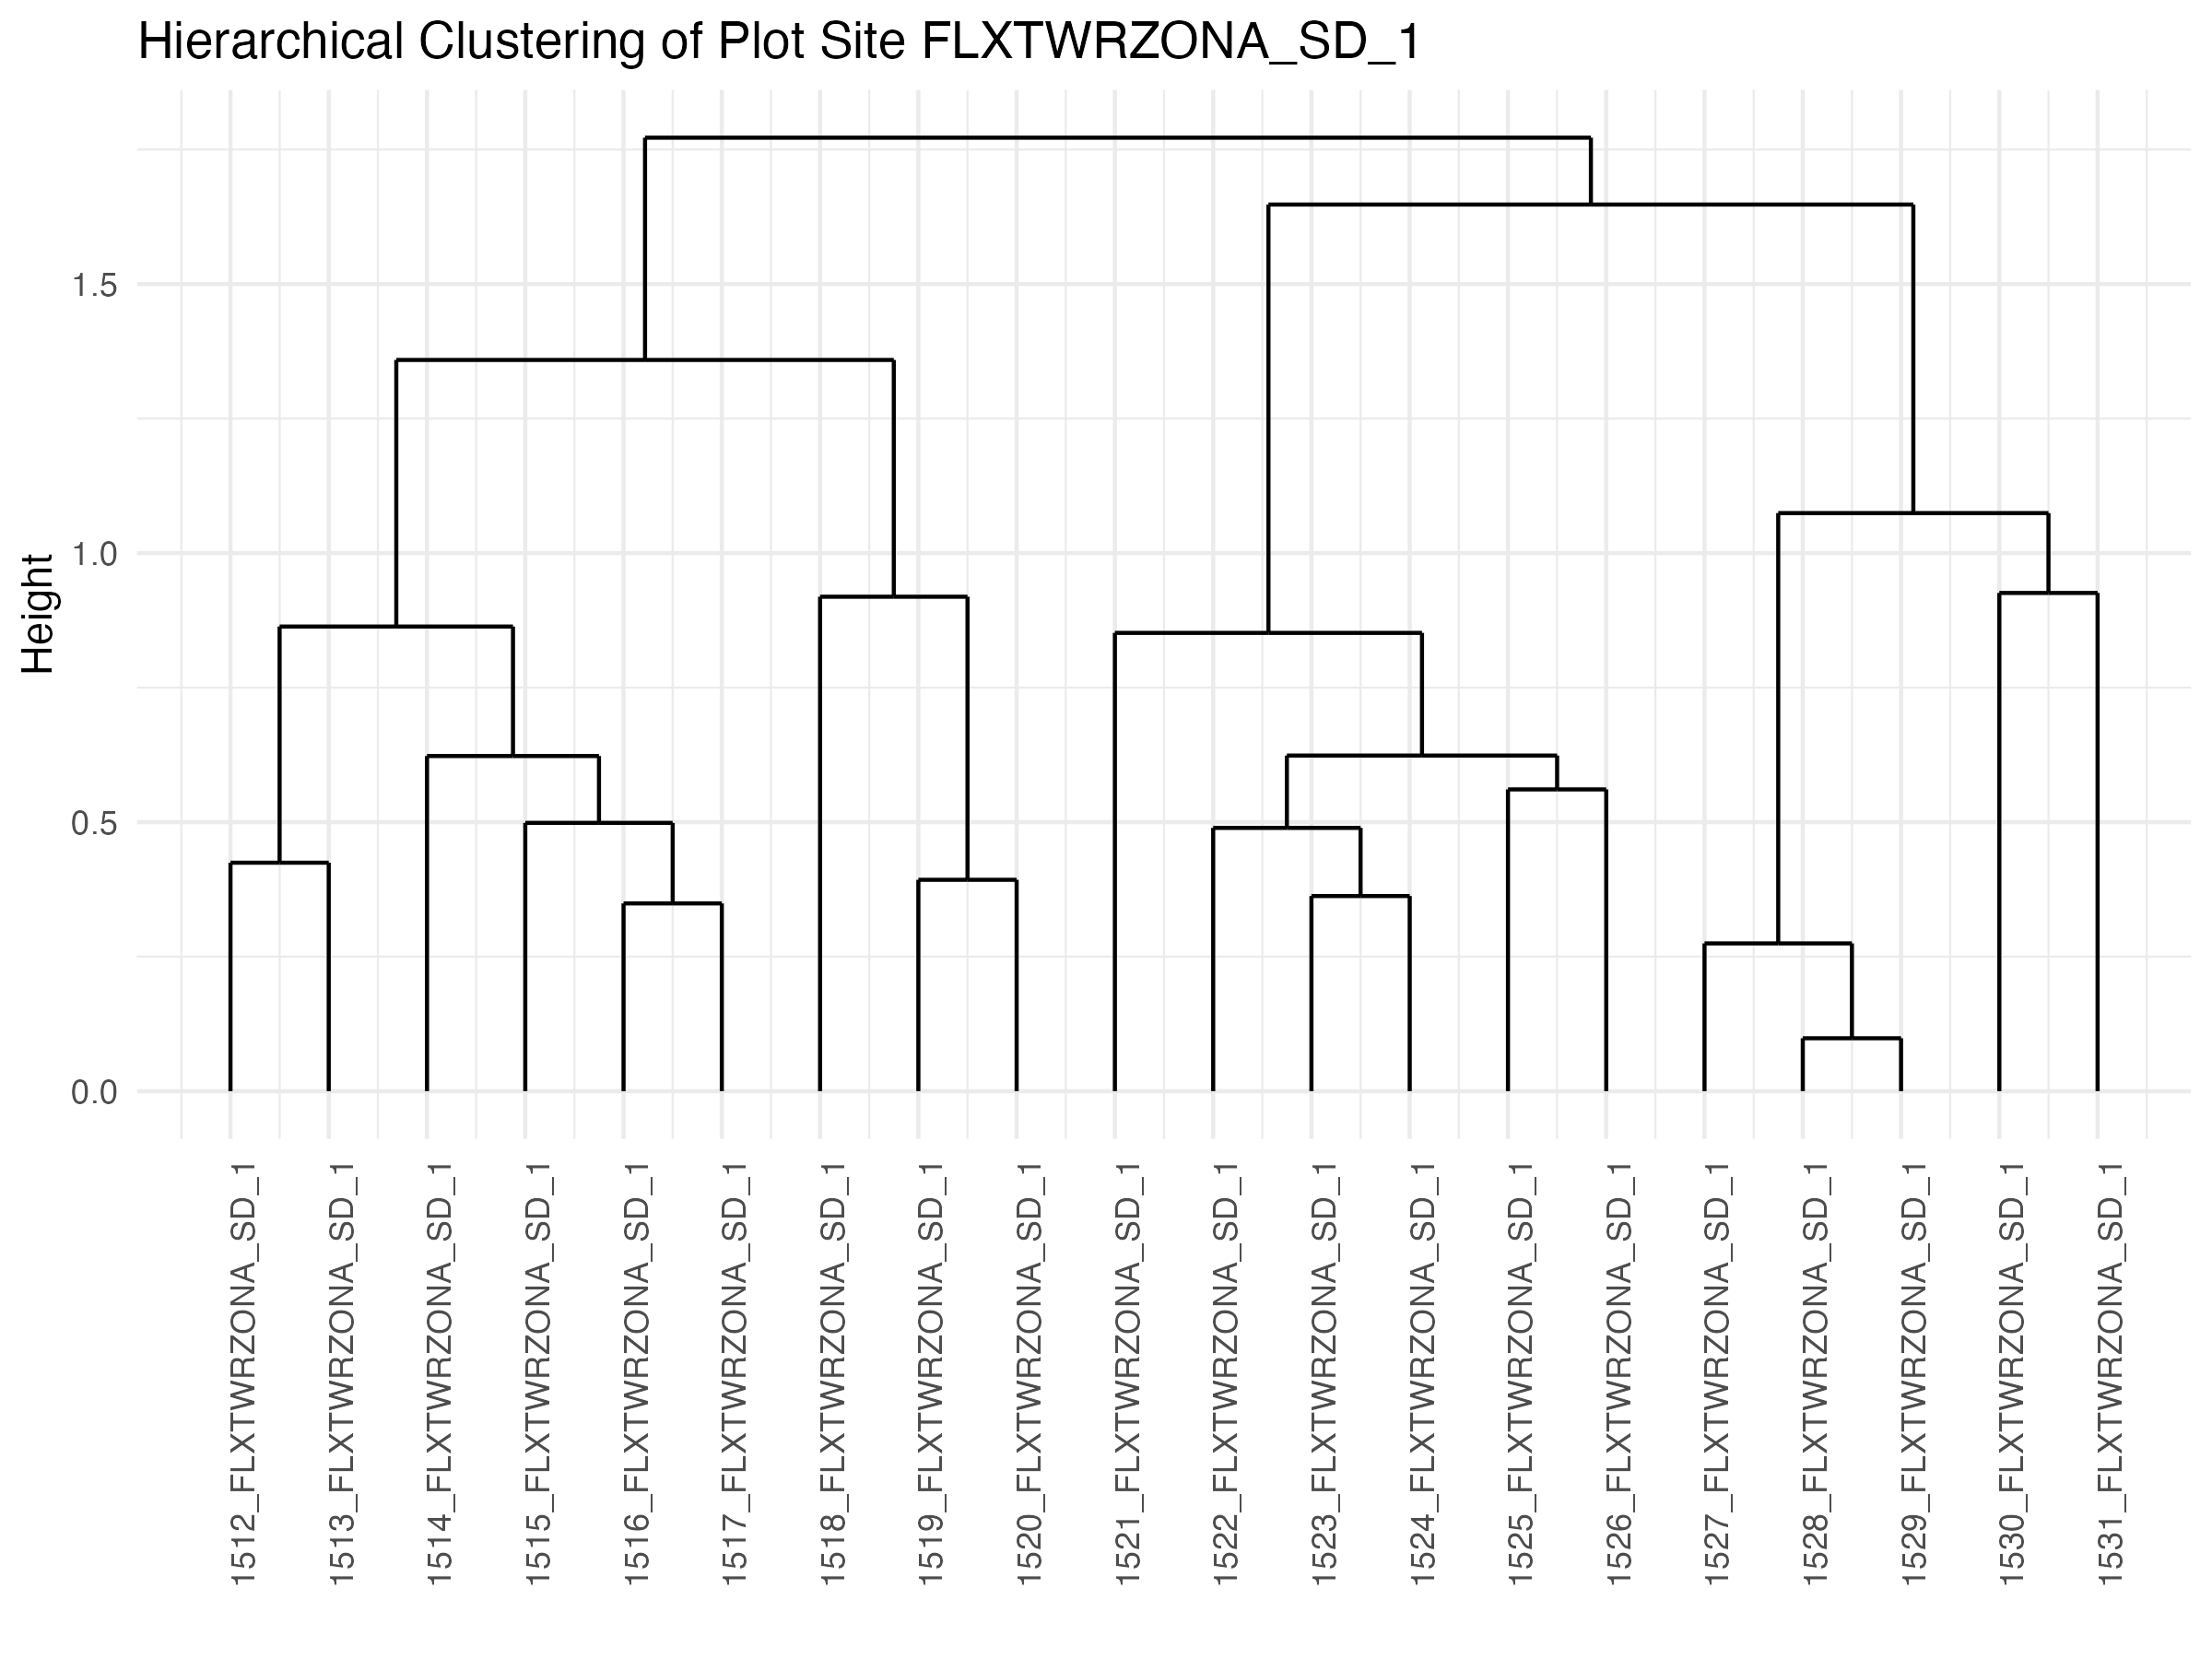
\includegraphics[width=0.9\textwidth]{Figures/Appendix/PlantCommunityClustering/FLXTWRZONA_SD_1_DENDRO.png} % Replace with your actual image path
    \caption{Community cluster dendrogram plot for test site FLXTWRZONA\_SD\_1}
    \label{fig:FLXTWRZONA_SD_1_DENDRO}
\end{figure}

\subsection{FLXTWRZONA\_SD\_2}
\begin{figure}[H]
    \centering
    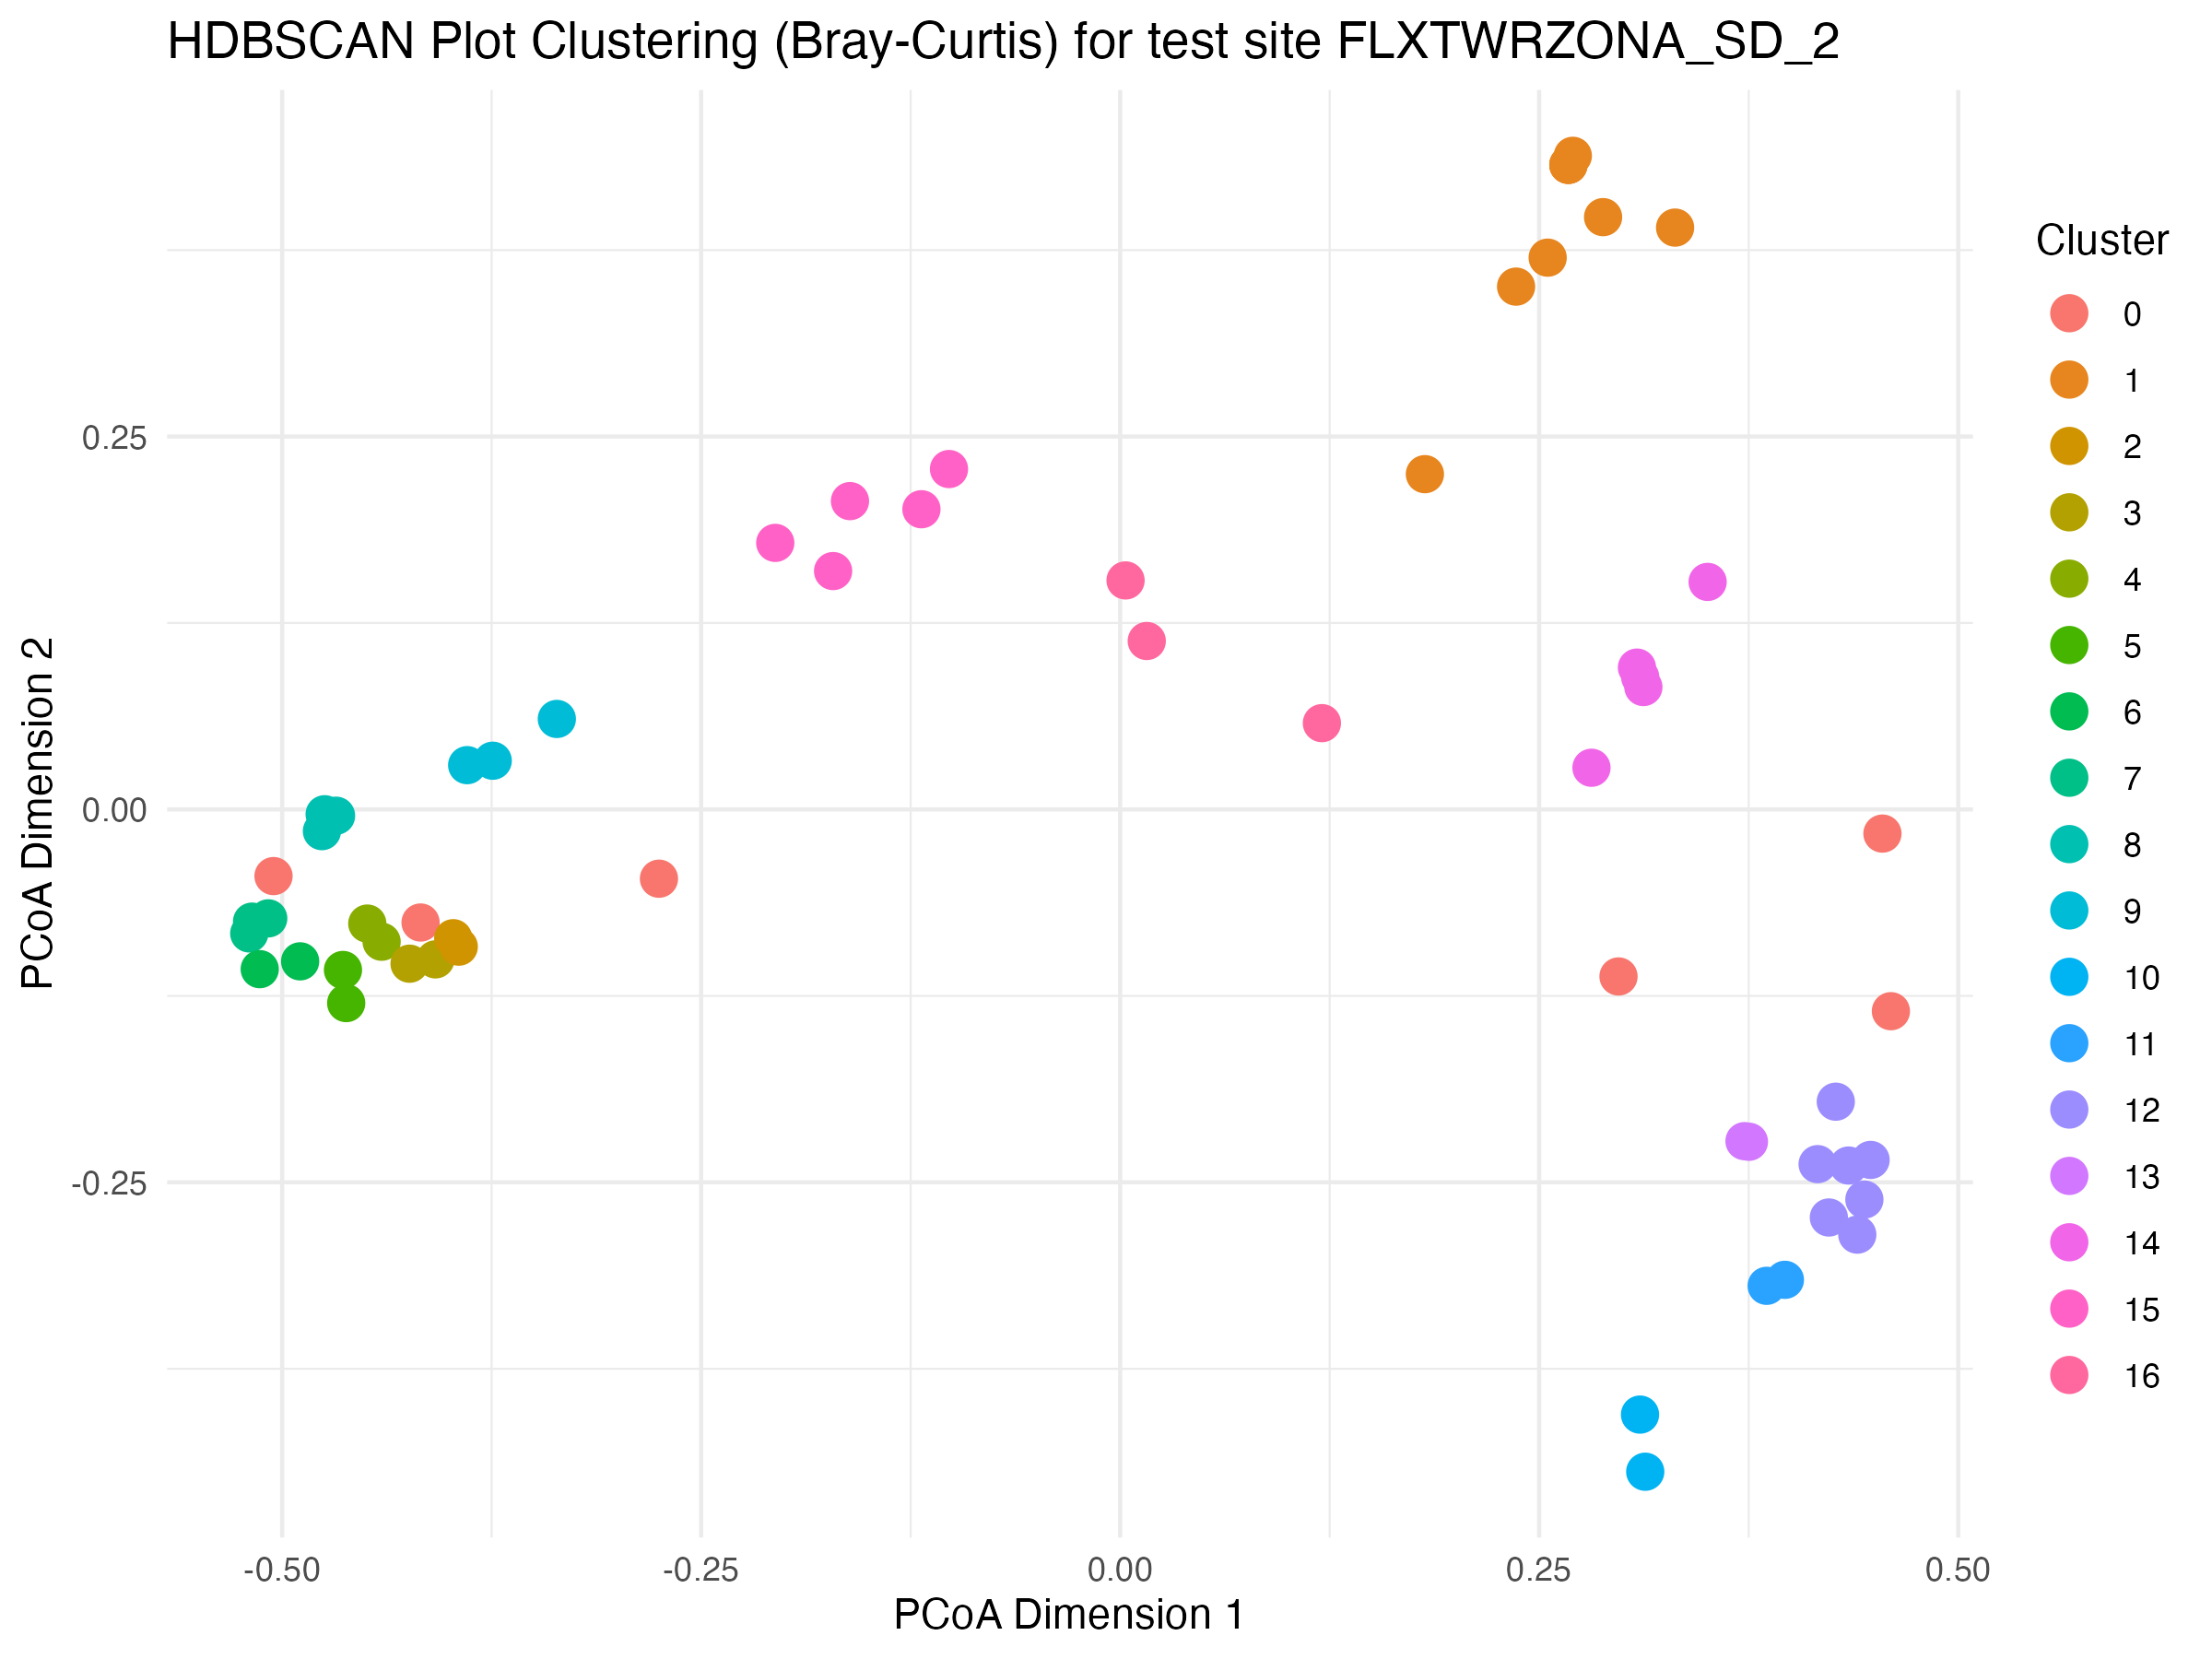
\includegraphics[width=0.9\textwidth]{Figures/Appendix/PlantCommunityClustering/FLXTWRZONA_SD_2_HDBSCAN_clusters.png} % Replace with your actual image path
    \caption{Community cluster HDBSCAN plot for test site FLXTWRZONA\_SD\_2}
    \label{fig:FLXTWRZONA_SD_2_HDBSCAN_clusters}
\end{figure}

\begin{figure}[H]
    \centering
    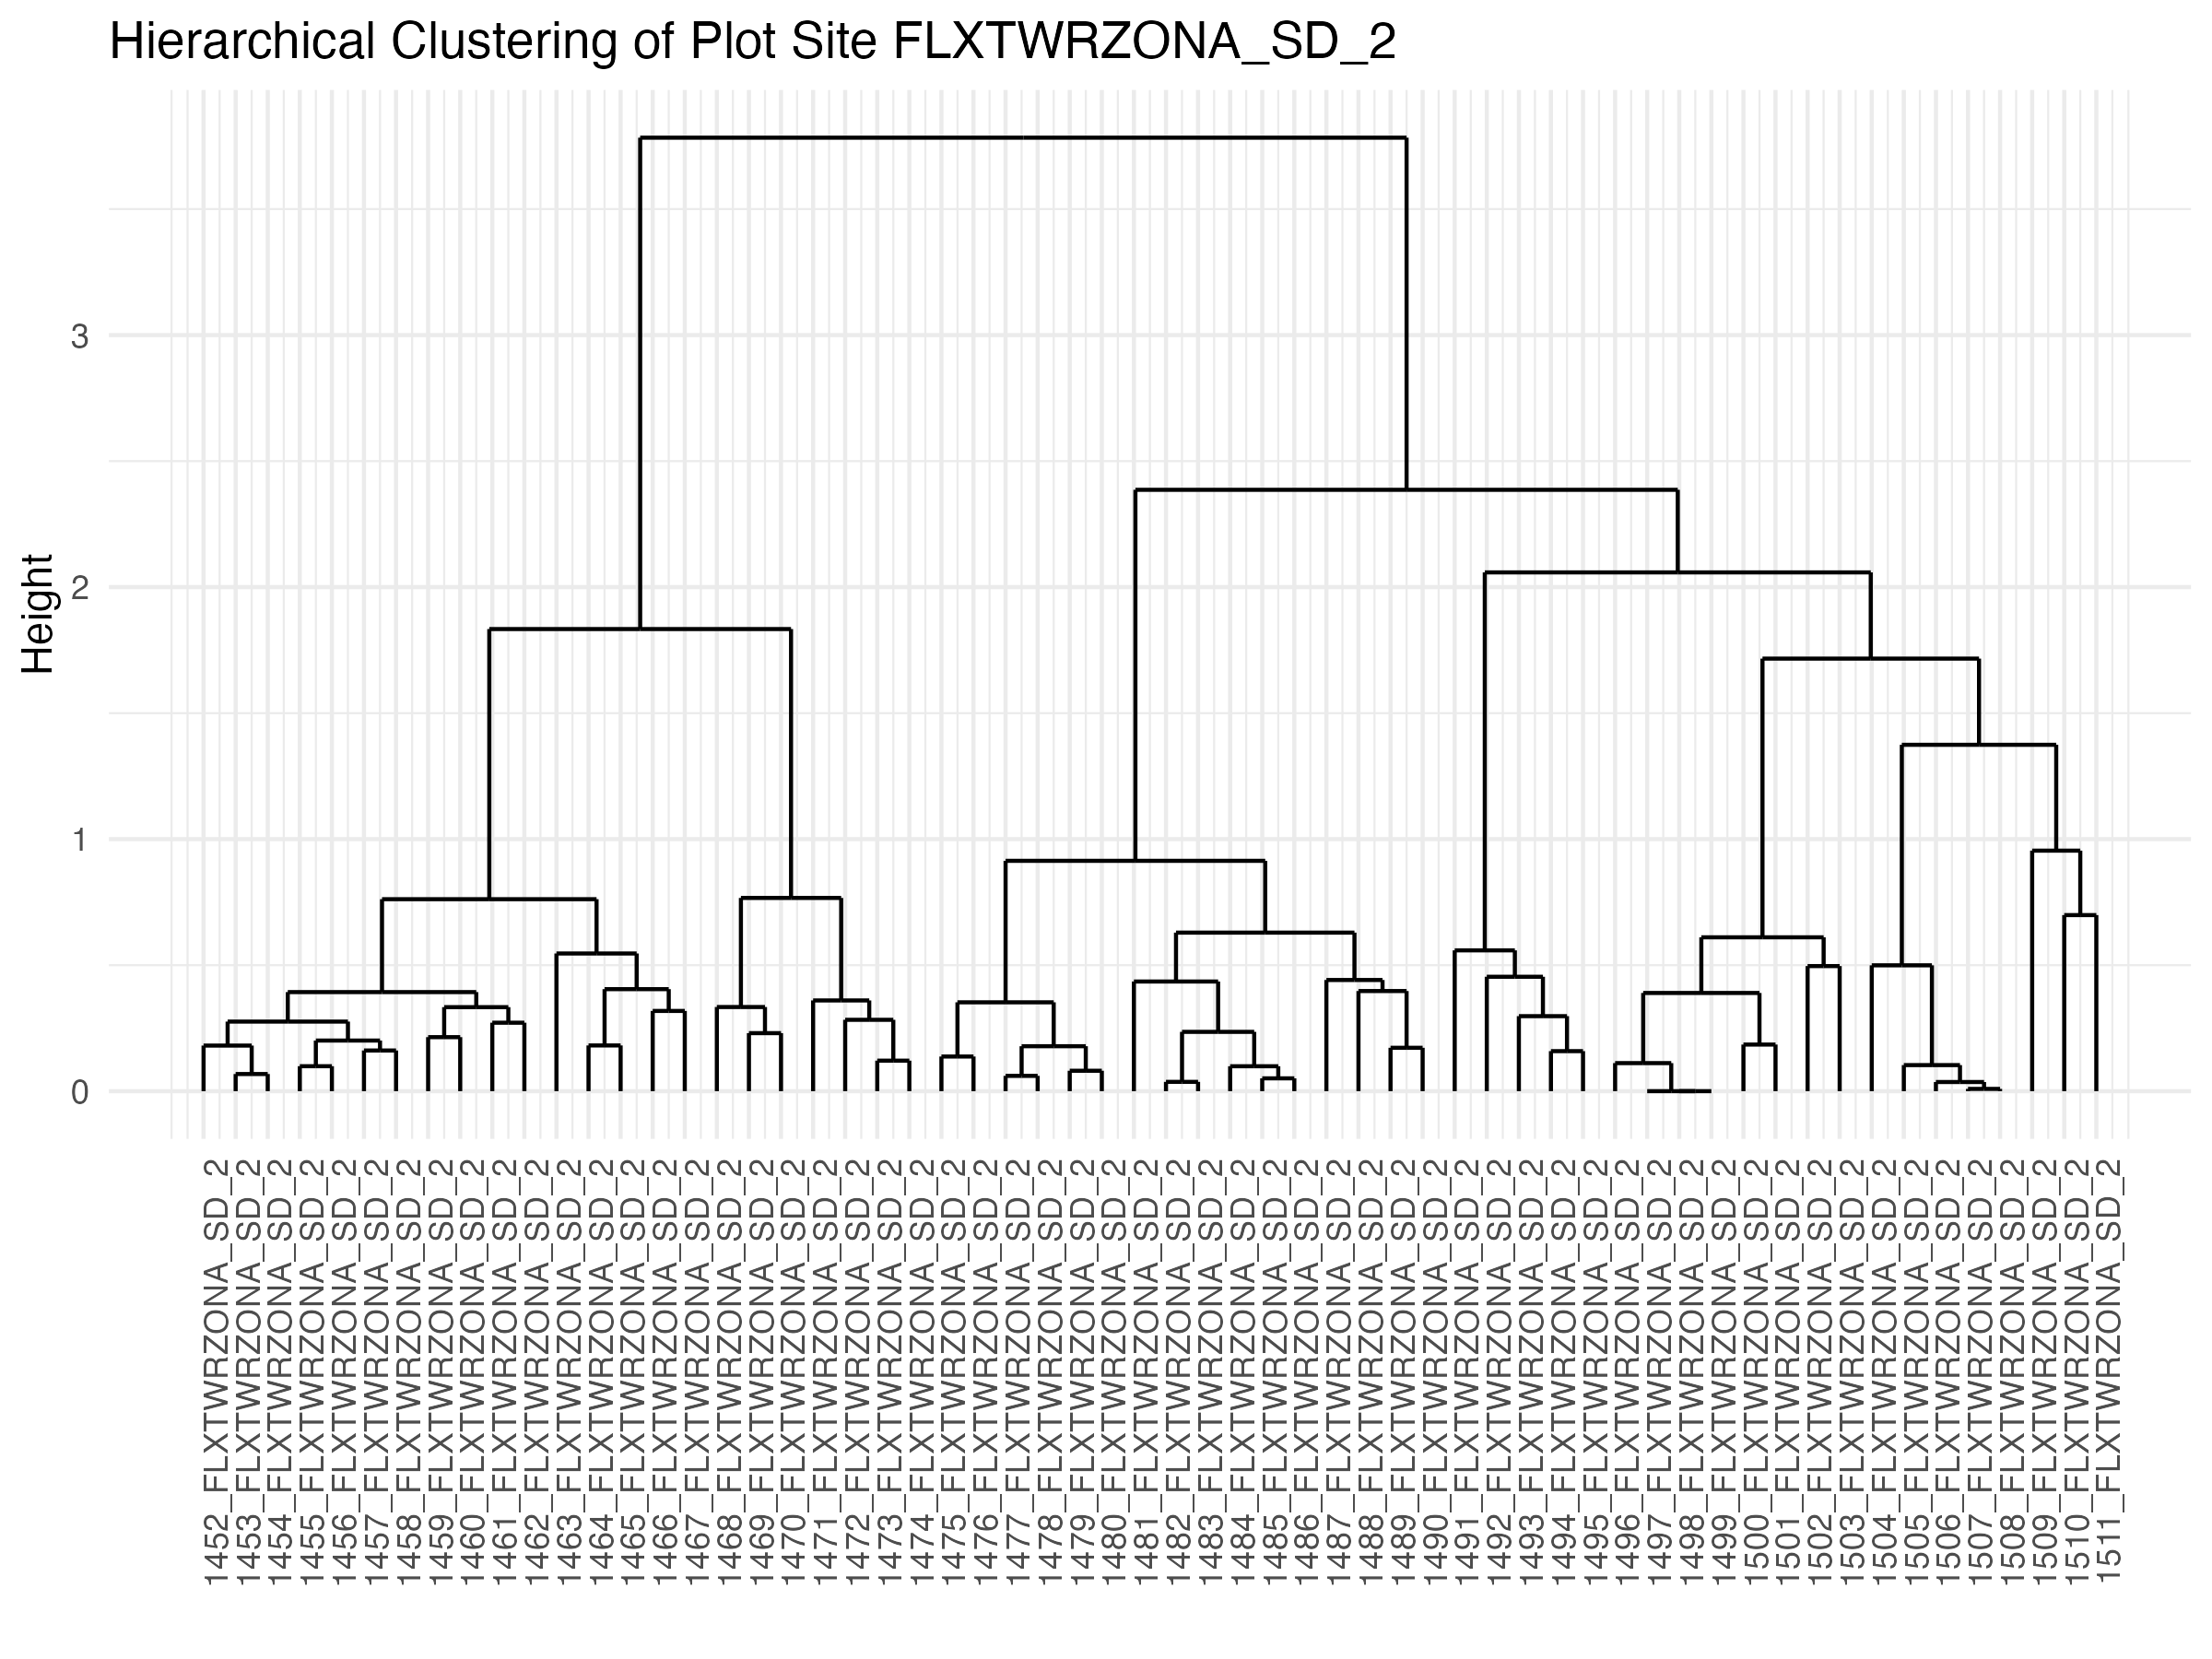
\includegraphics[width=0.9\textwidth]{Figures/Appendix/PlantCommunityClustering/FLXTWRZONA_SD_2_DENDRO.png} % Replace with your actual image path
    \caption{Community cluster dendrogram plot for test site FLXTWRZONA\_SD\_2}
    \label{fig:FLXTWRZONA_SD_2_DENDRO}
\end{figure}

\subsection{FLXTWRZONA\_SD\_3}
\begin{figure}[H]
    \centering
    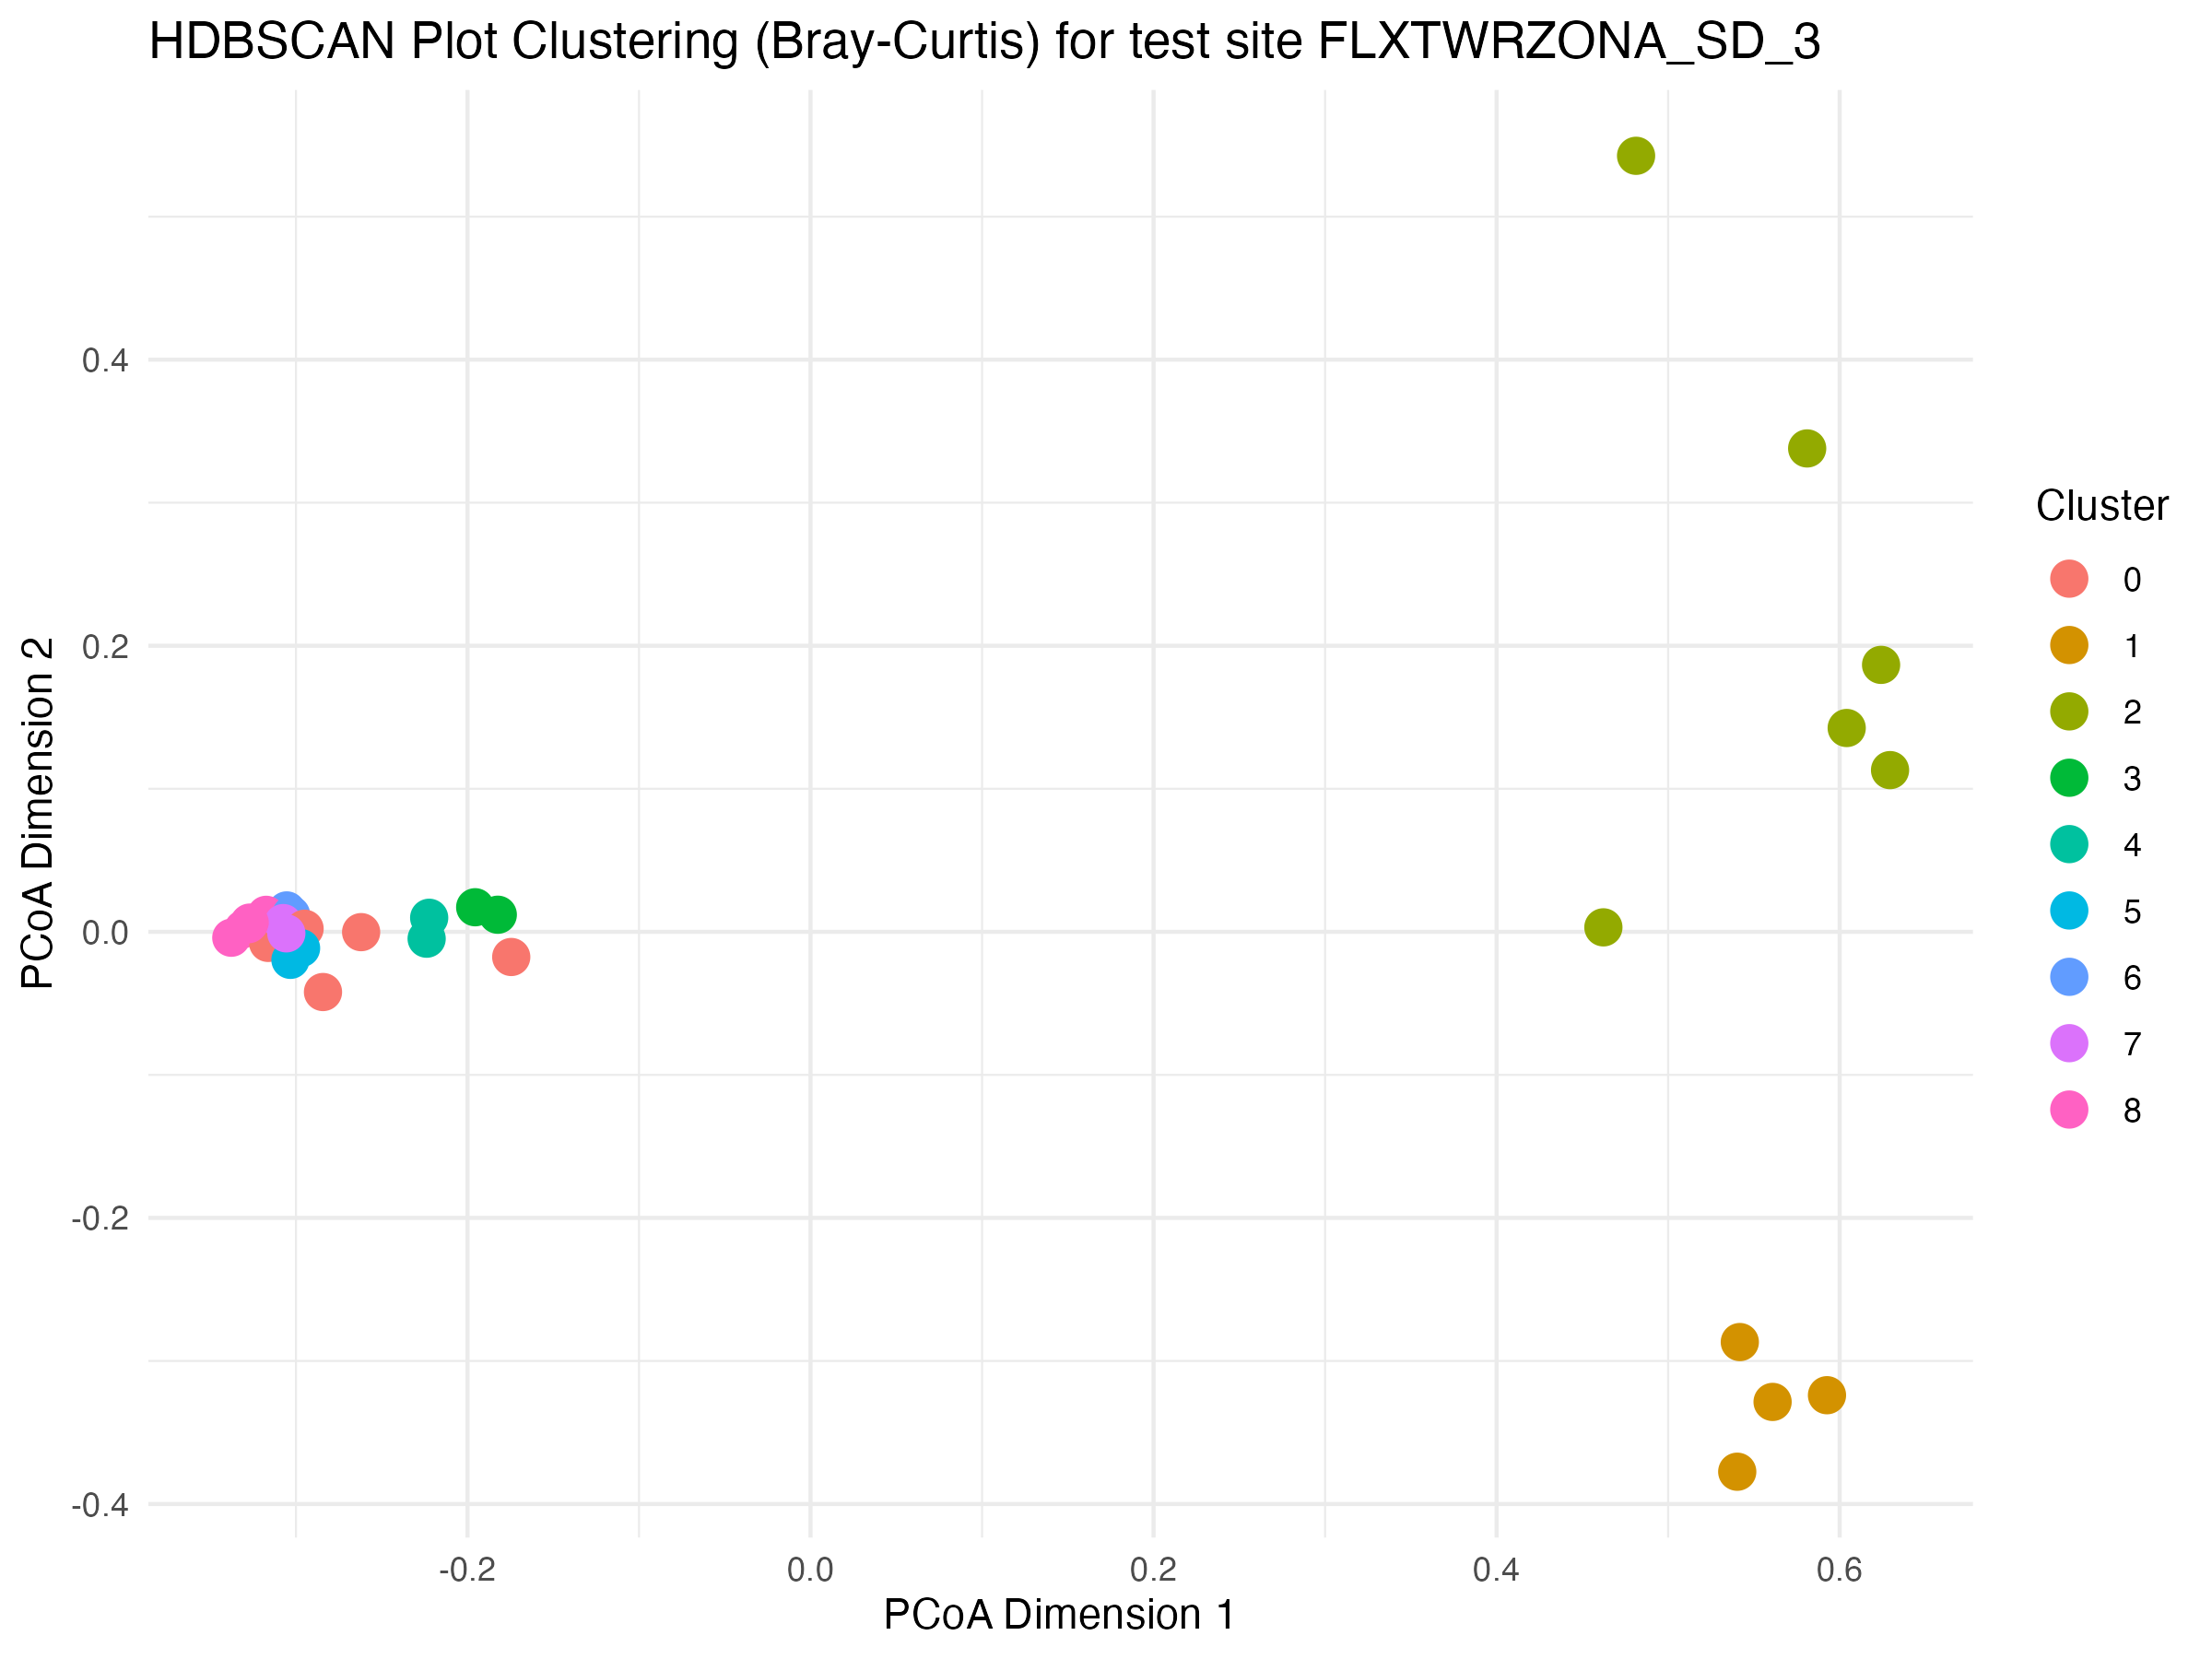
\includegraphics[width=0.9\textwidth]{Figures/Appendix/PlantCommunityClustering/FLXTWRZONA_SD_3_HDBSCAN_clusters.png} % Replace with your actual image path
    \caption{Community cluster HDBSCAN plot for test site FLXTWRZONA\_SD\_3}
    \label{fig:FLXTWRZONA_SD_3_HDBSCAN_clusters}
\end{figure}

\begin{figure}[H]
    \centering
    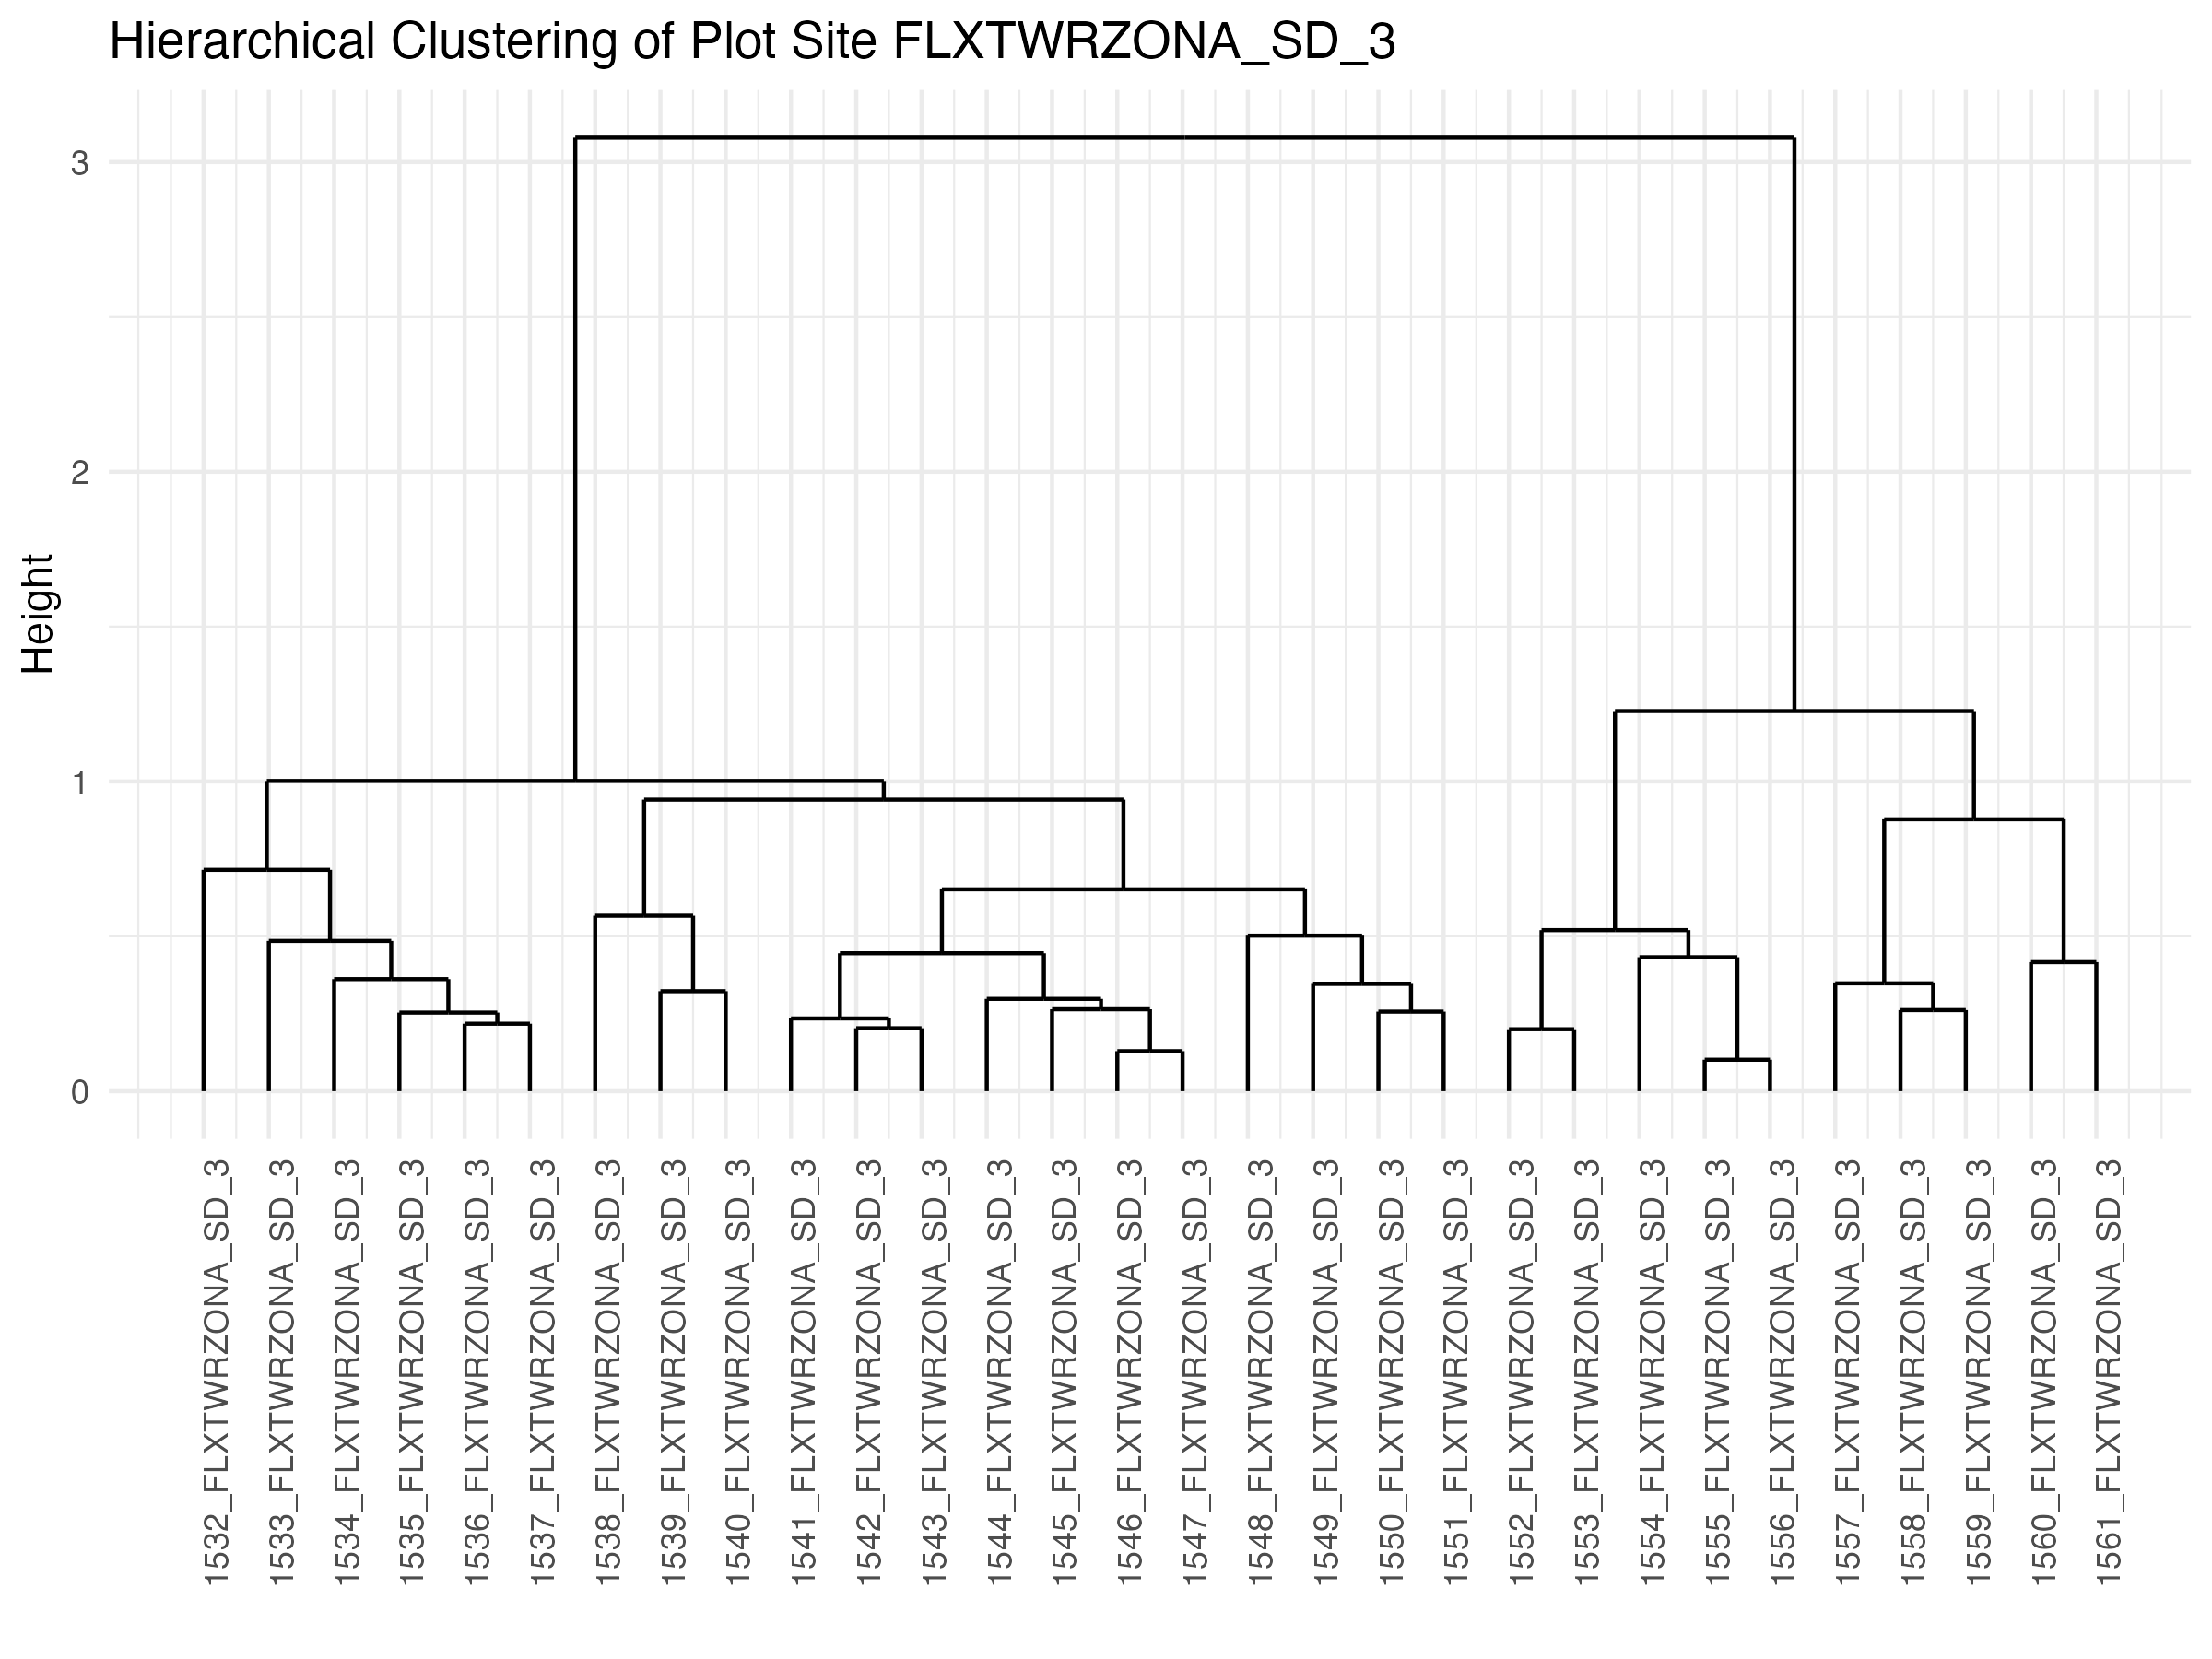
\includegraphics[width=0.9\textwidth]{Figures/Appendix/PlantCommunityClustering/FLXTWRZONA_SD_3_DENDRO.png} % Replace with your actual image path
    \caption{Community cluster dendrogram plot for test site FLXTWRZONA\_SD\_3}
    \label{fig:FLXTWRZONA_SD_3_DENDRO}
\end{figure}

\subsection{FLXTWRZONA\_SD\_4}
\begin{figure}[H]
    \centering
    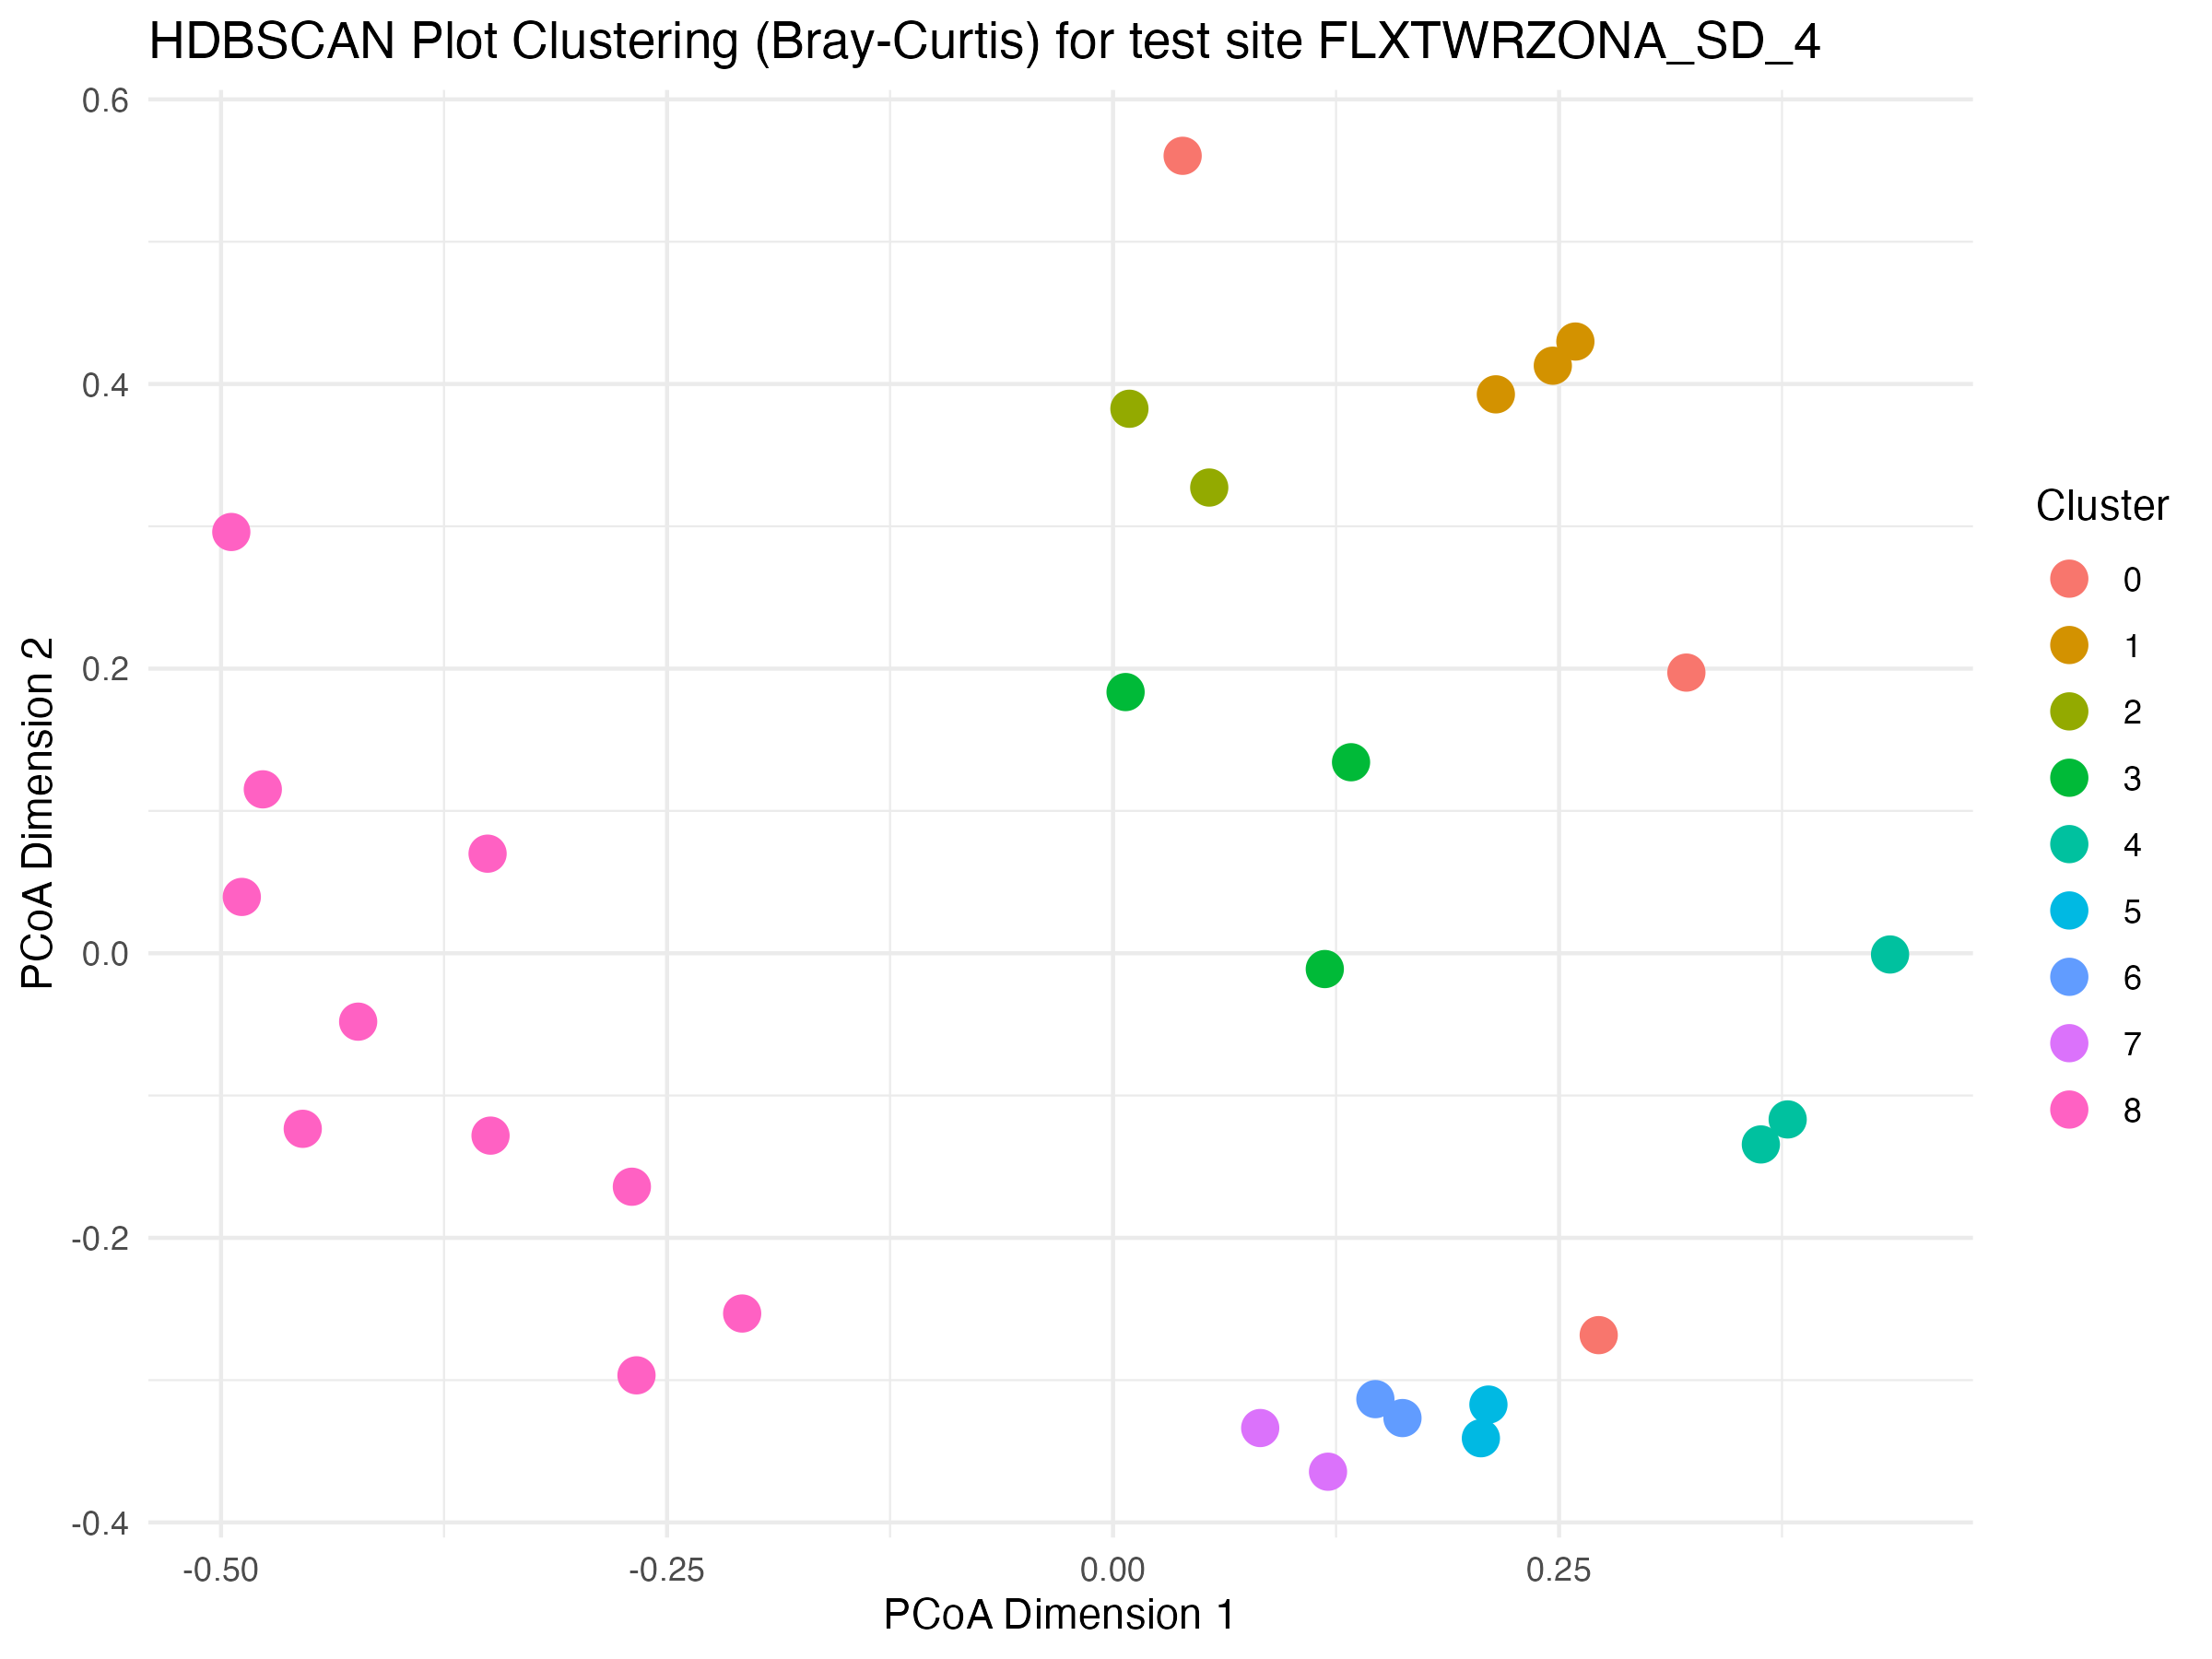
\includegraphics[width=0.9\textwidth]{Figures/Appendix/PlantCommunityClustering/FLXTWRZONA_SD_4_HDBSCAN_clusters.png} % Replace with your actual image path
    \caption{Community cluster HDBSCAN plot for test site FLXTWRZONA\_SD\_4}
    \label{fig:FLXTWRZONA_SD_4_HDBSCAN_clusters}
\end{figure}

\begin{figure}[H]
    \centering
    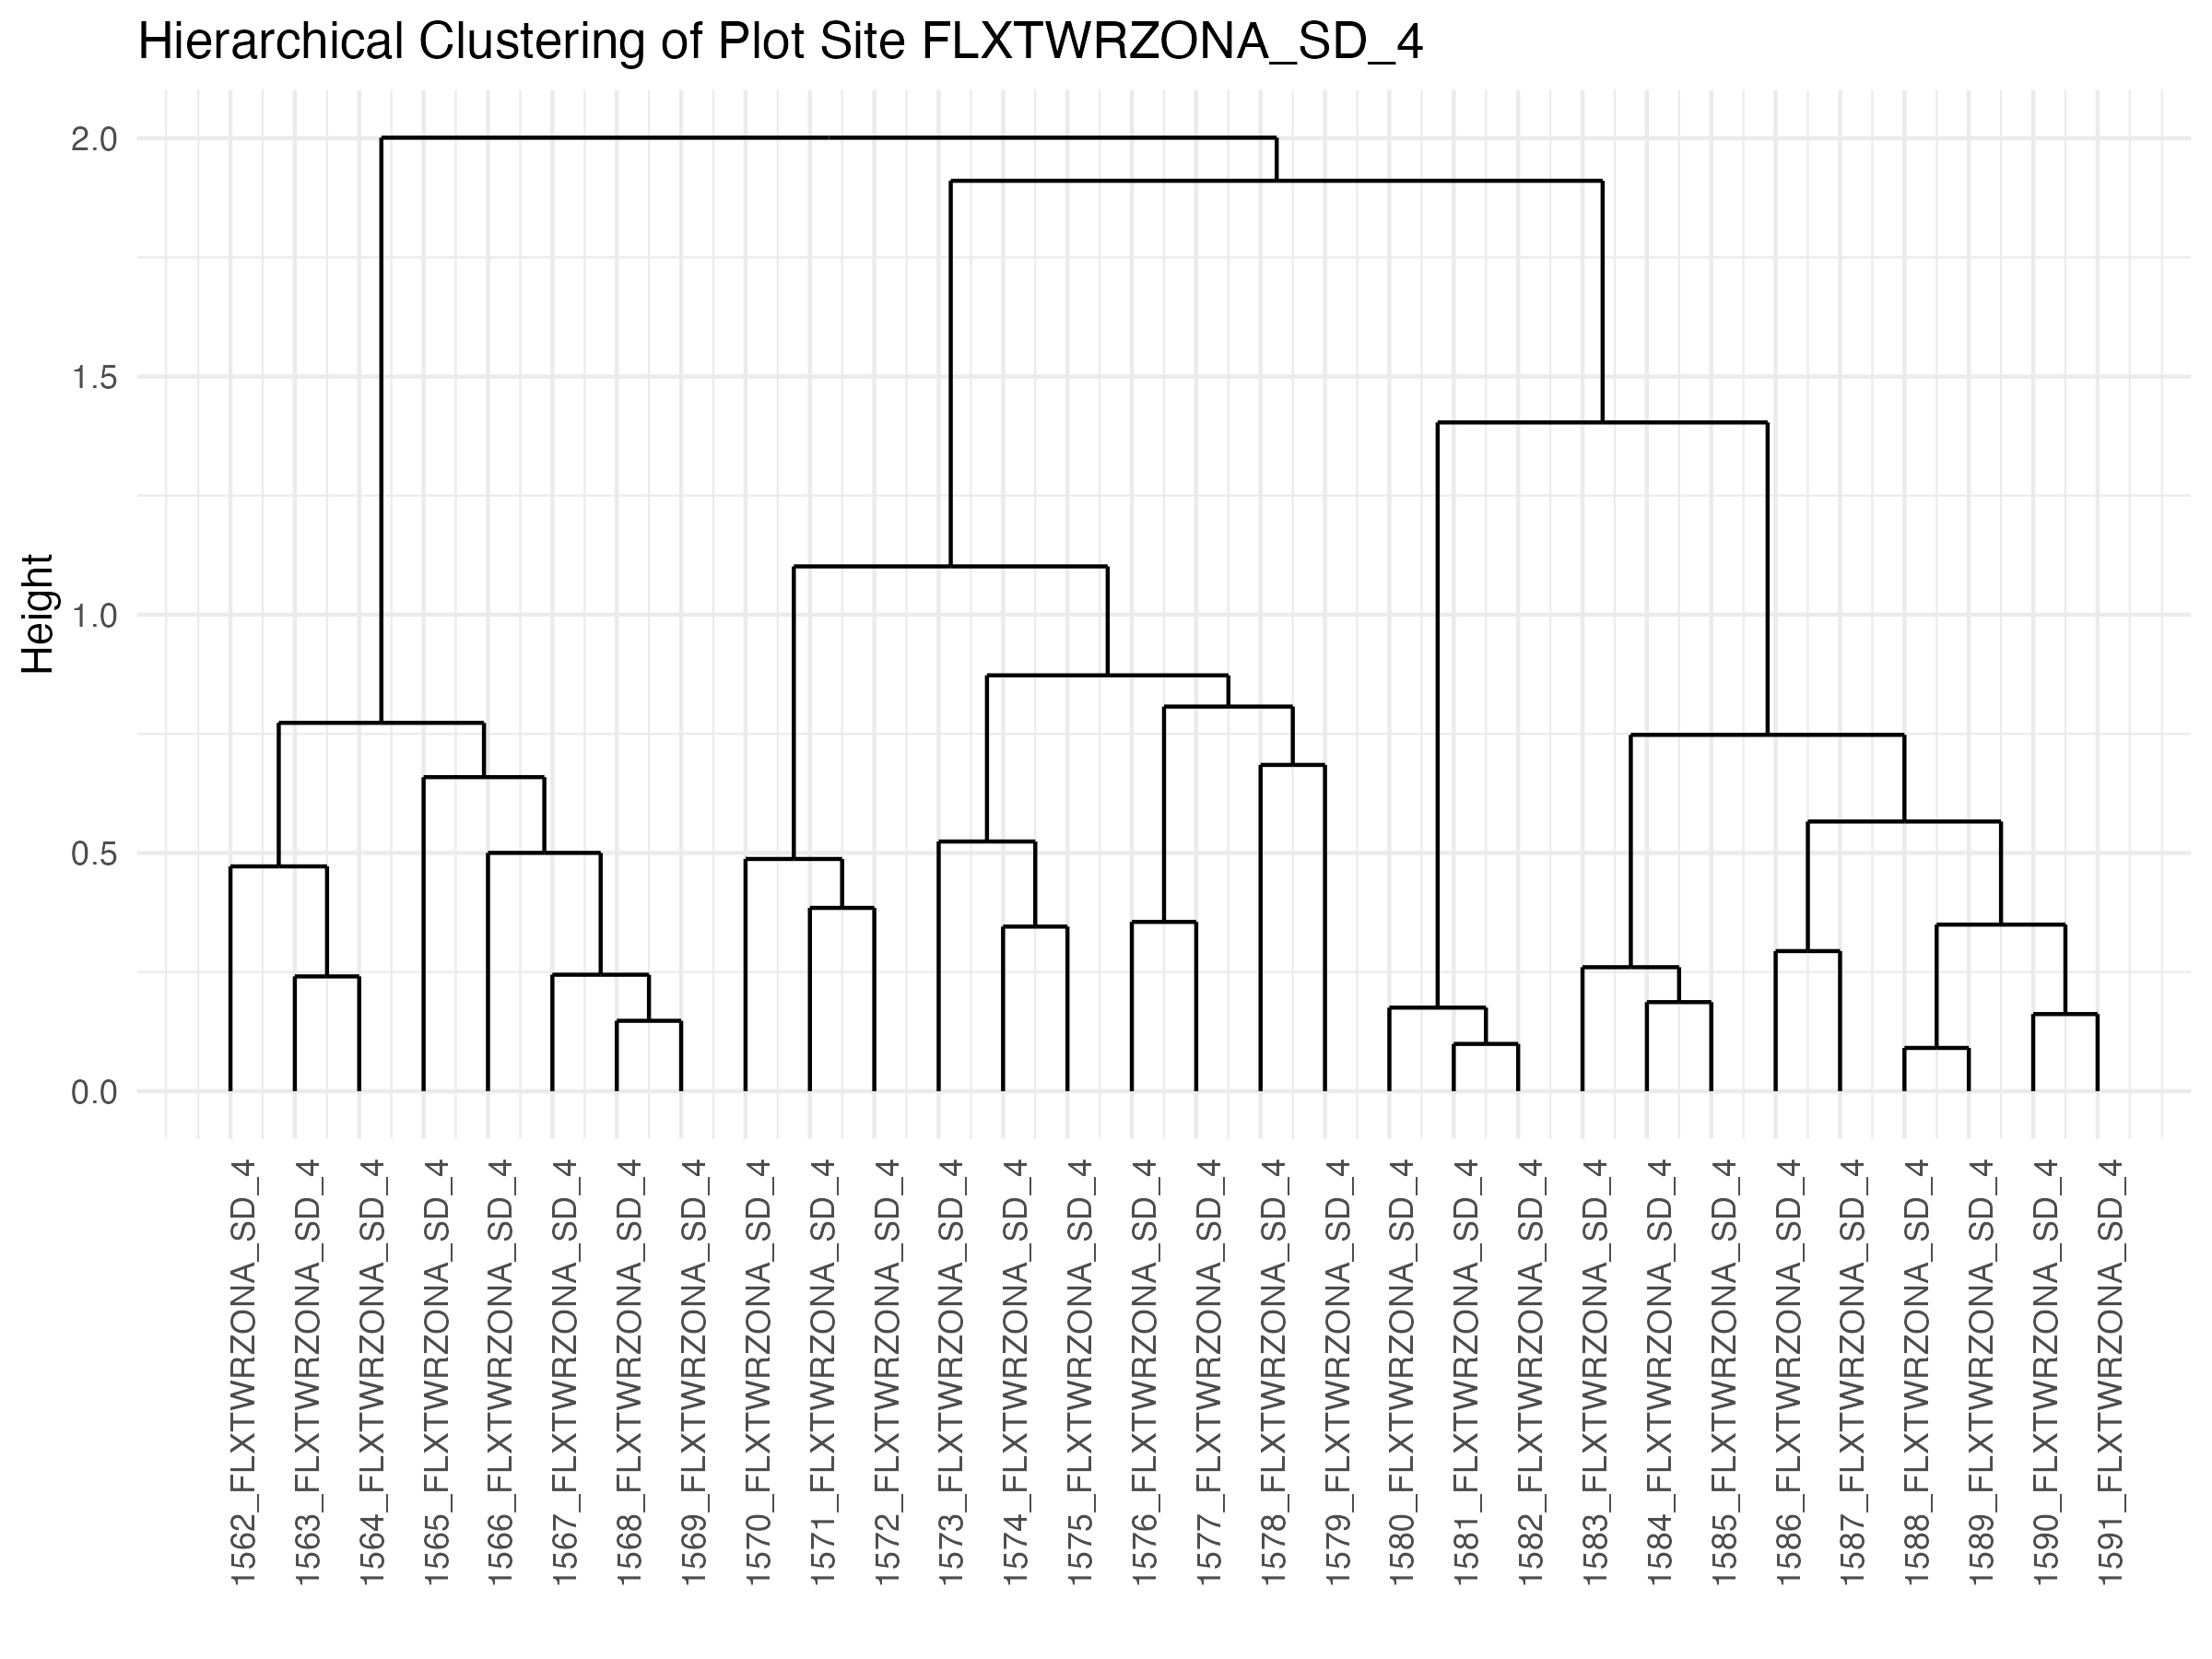
\includegraphics[width=0.9\textwidth]{Figures/Appendix/PlantCommunityClustering/FLXTWRZONA_SD_4_DENDRO.png} % Replace with your actual image path
    \caption{Community cluster dendrogram plot for test site FLXTWRZONA\_SD\_4}
    \label{fig:FLXTWRZONA_SD_4_DENDRO}
\end{figure}

\subsection{FRST\_AK\_2}
\begin{figure}[H]
    \centering
    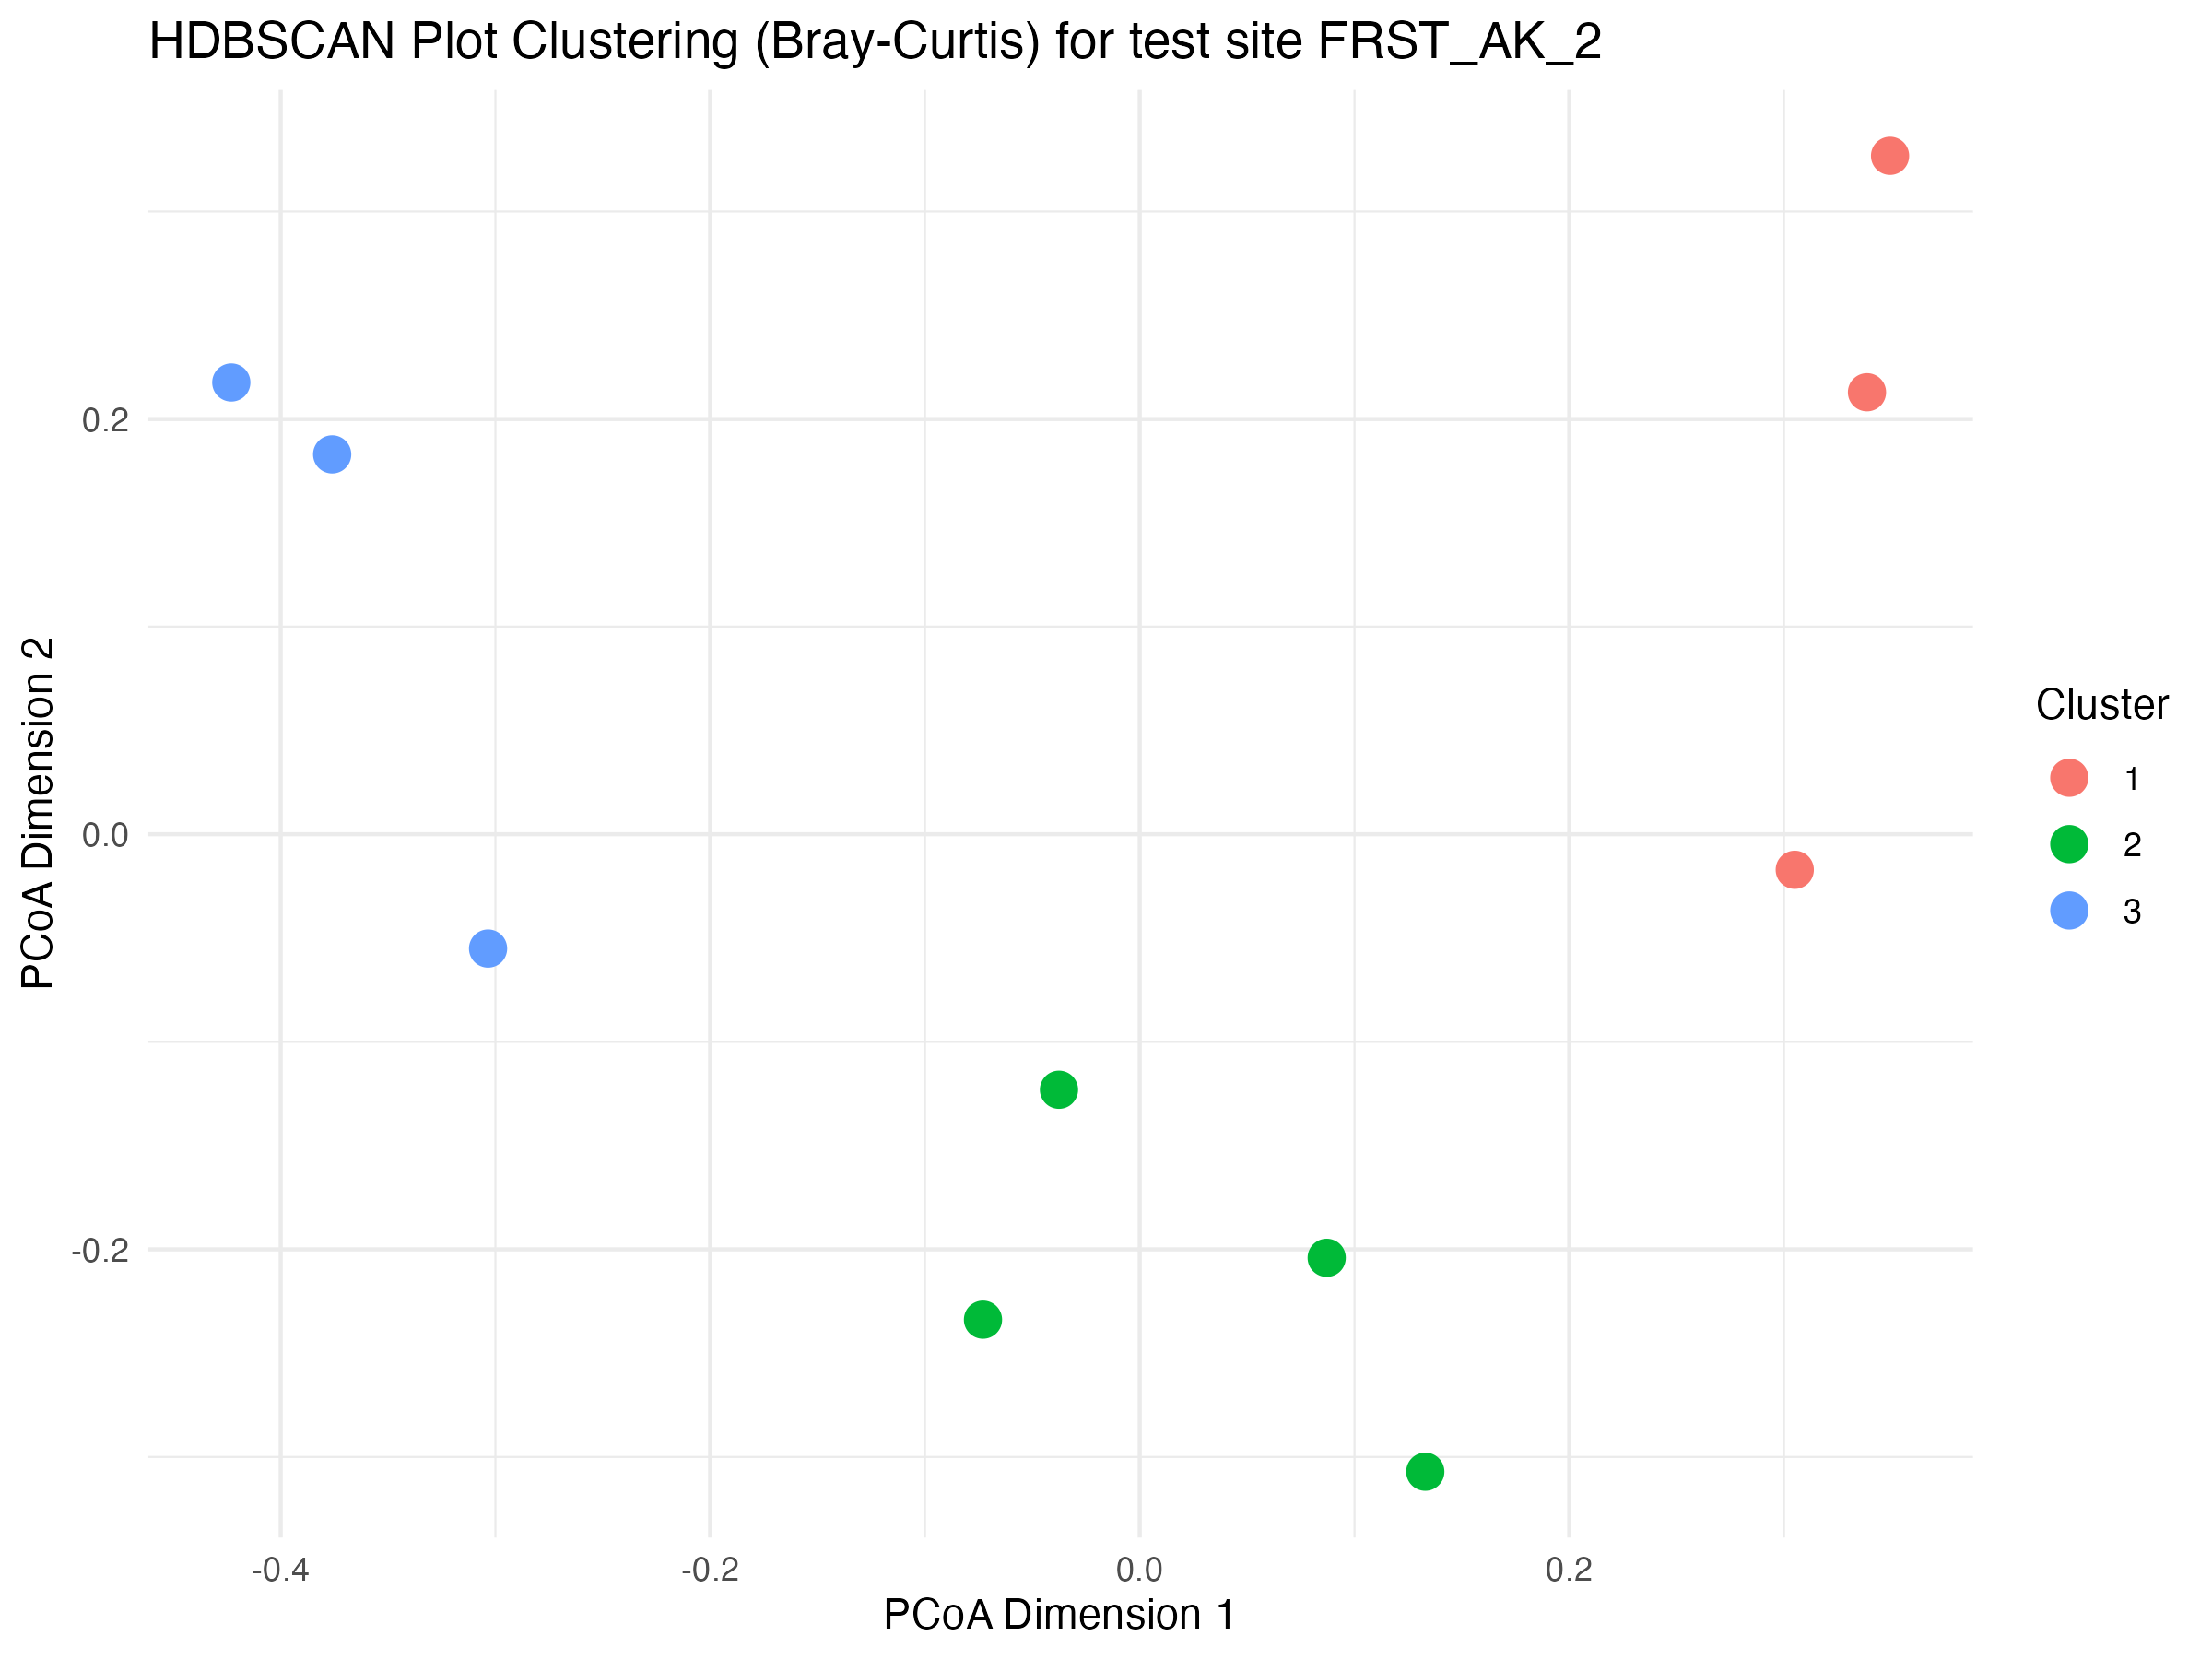
\includegraphics[width=0.9\textwidth]{Figures/Appendix/PlantCommunityClustering/FRST_AK_2_HDBSCAN_clusters.png} % Replace with your actual image path
    \caption{Community cluster HDBSCAN plot for test site FRST\_AK\_2}
    \label{fig:FRST_AK_2_HDBSCAN_clusters}
\end{figure}

\begin{figure}[H]
    \centering
    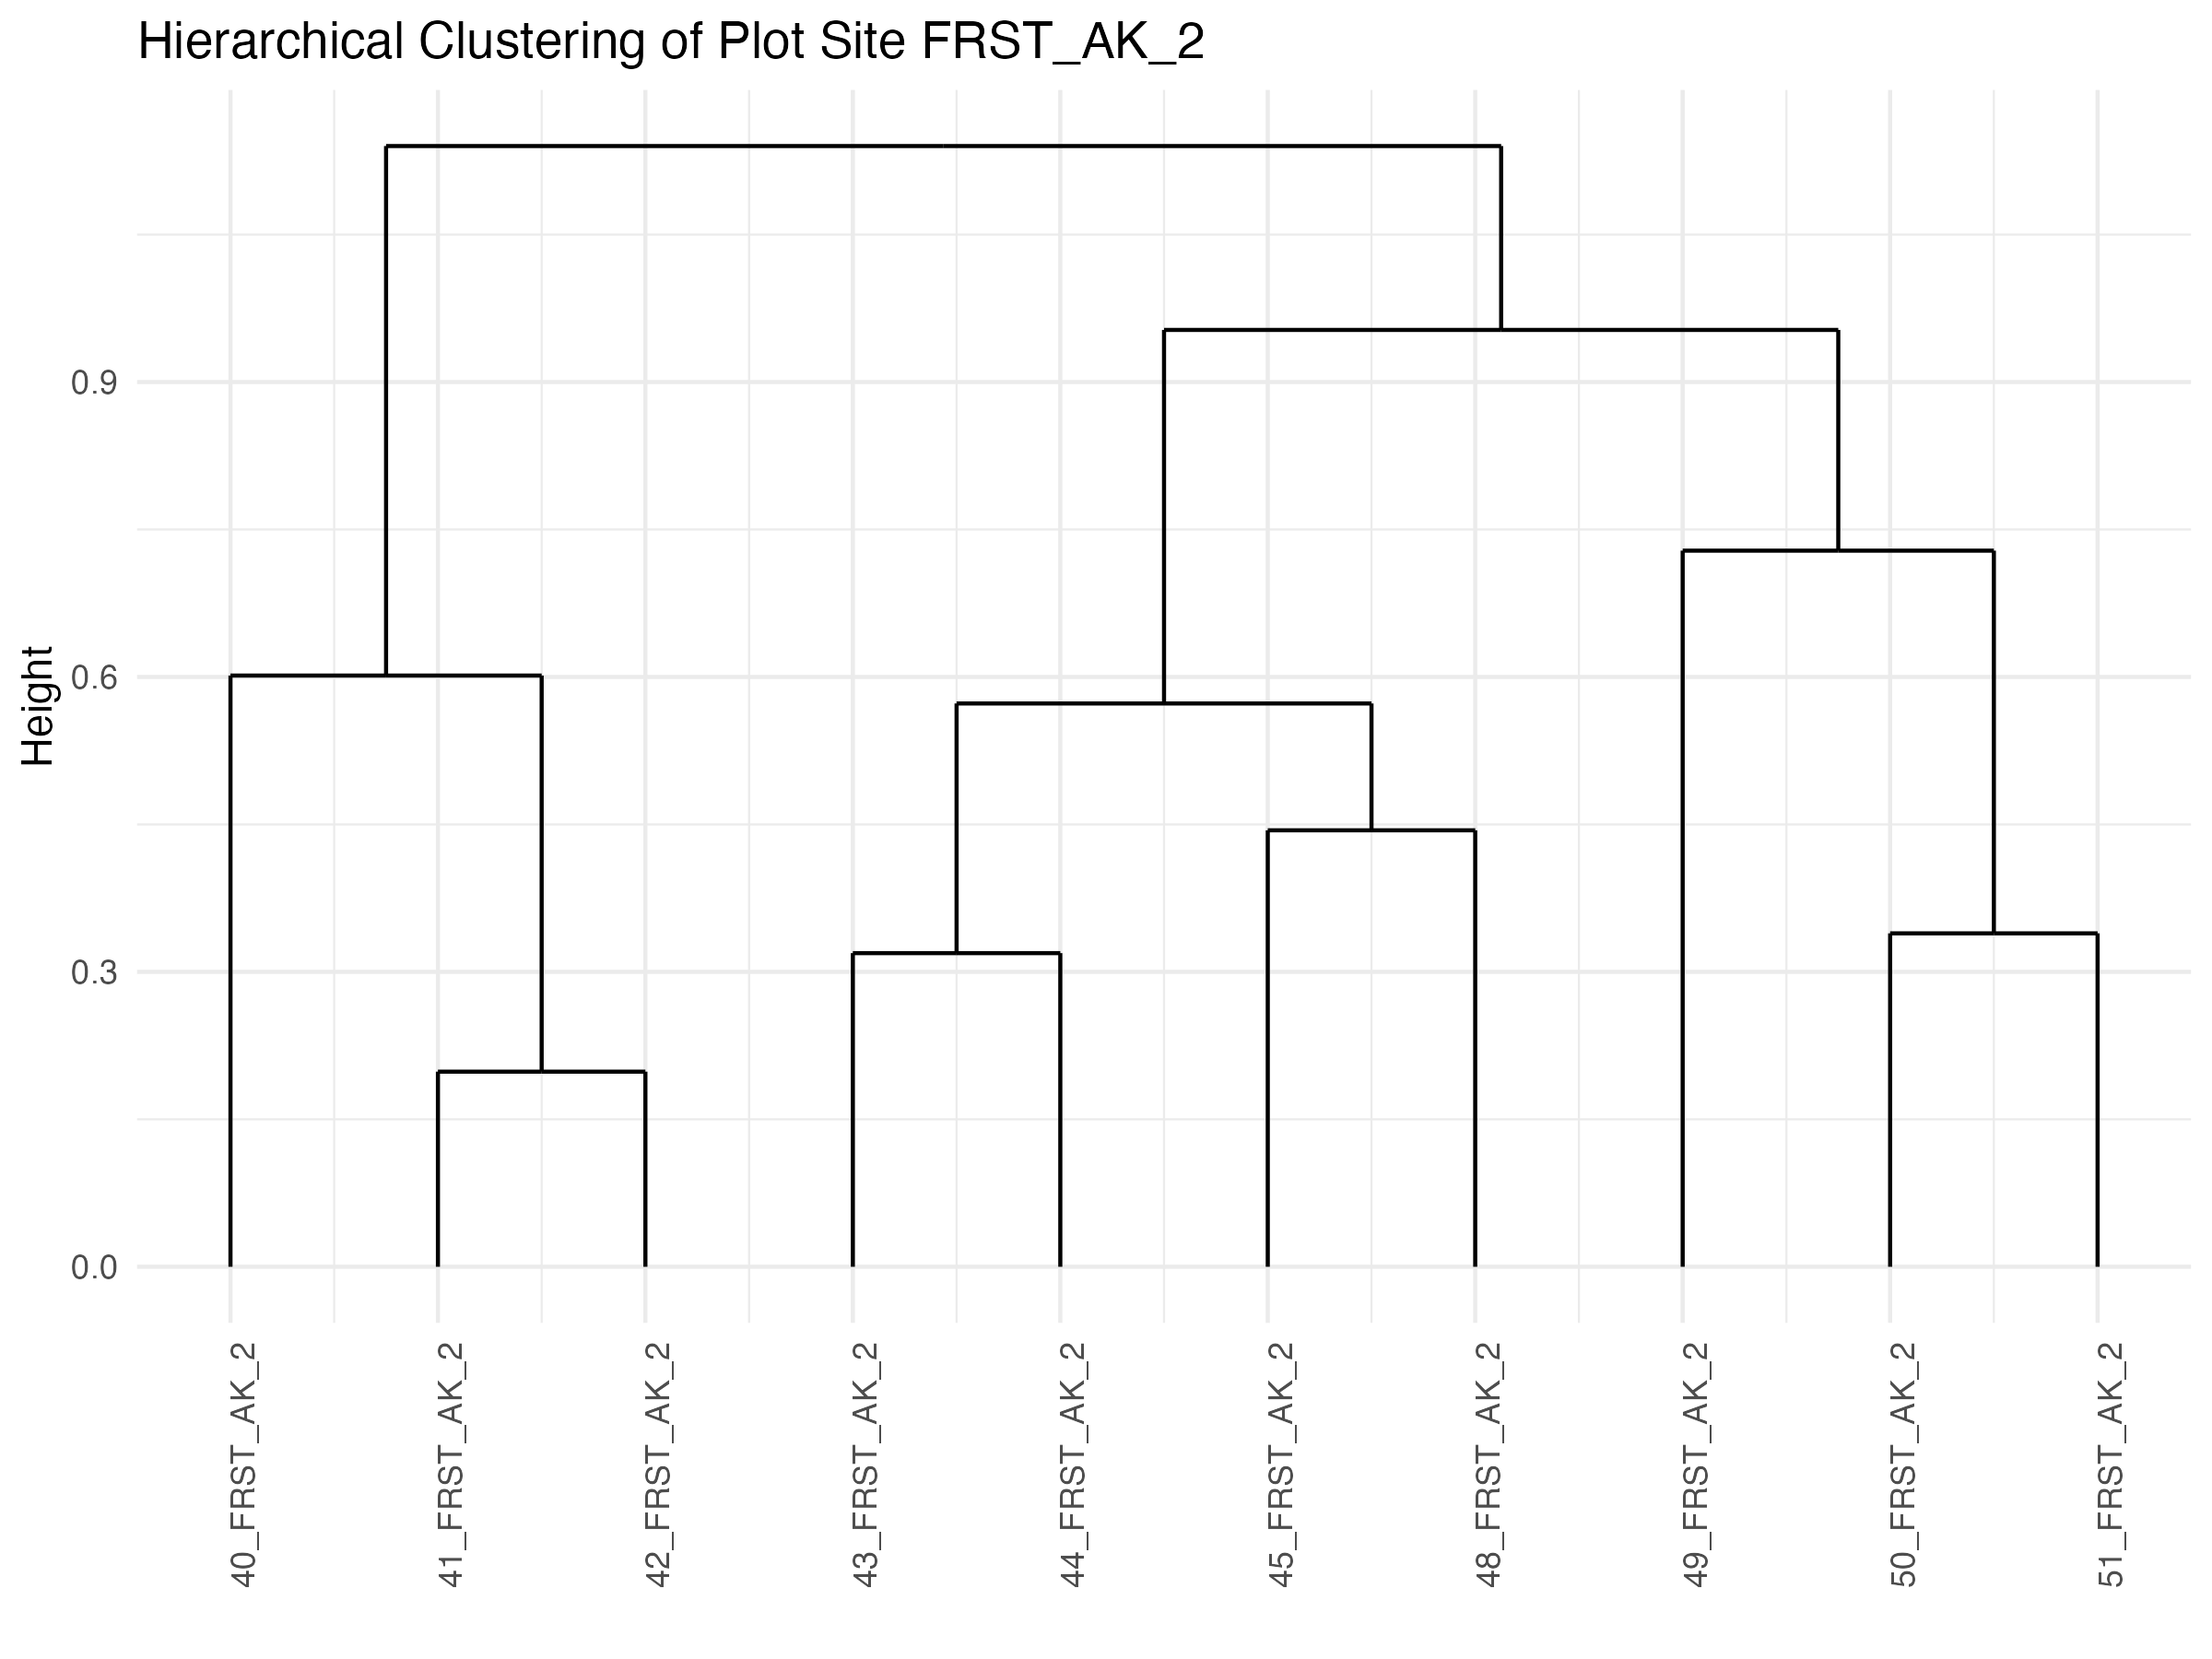
\includegraphics[width=0.9\textwidth]{Figures/Appendix/PlantCommunityClustering/FRST_AK_2_DENDRO.png} % Replace with your actual image path
    \caption{Community cluster dendrogram plot for test site FRST\_AK\_2}
    \label{fig:FRST_AK_2_DENDRO}
\end{figure}

\subsection{FRST\_AK\_3}
\begin{figure}[H]
    \centering
    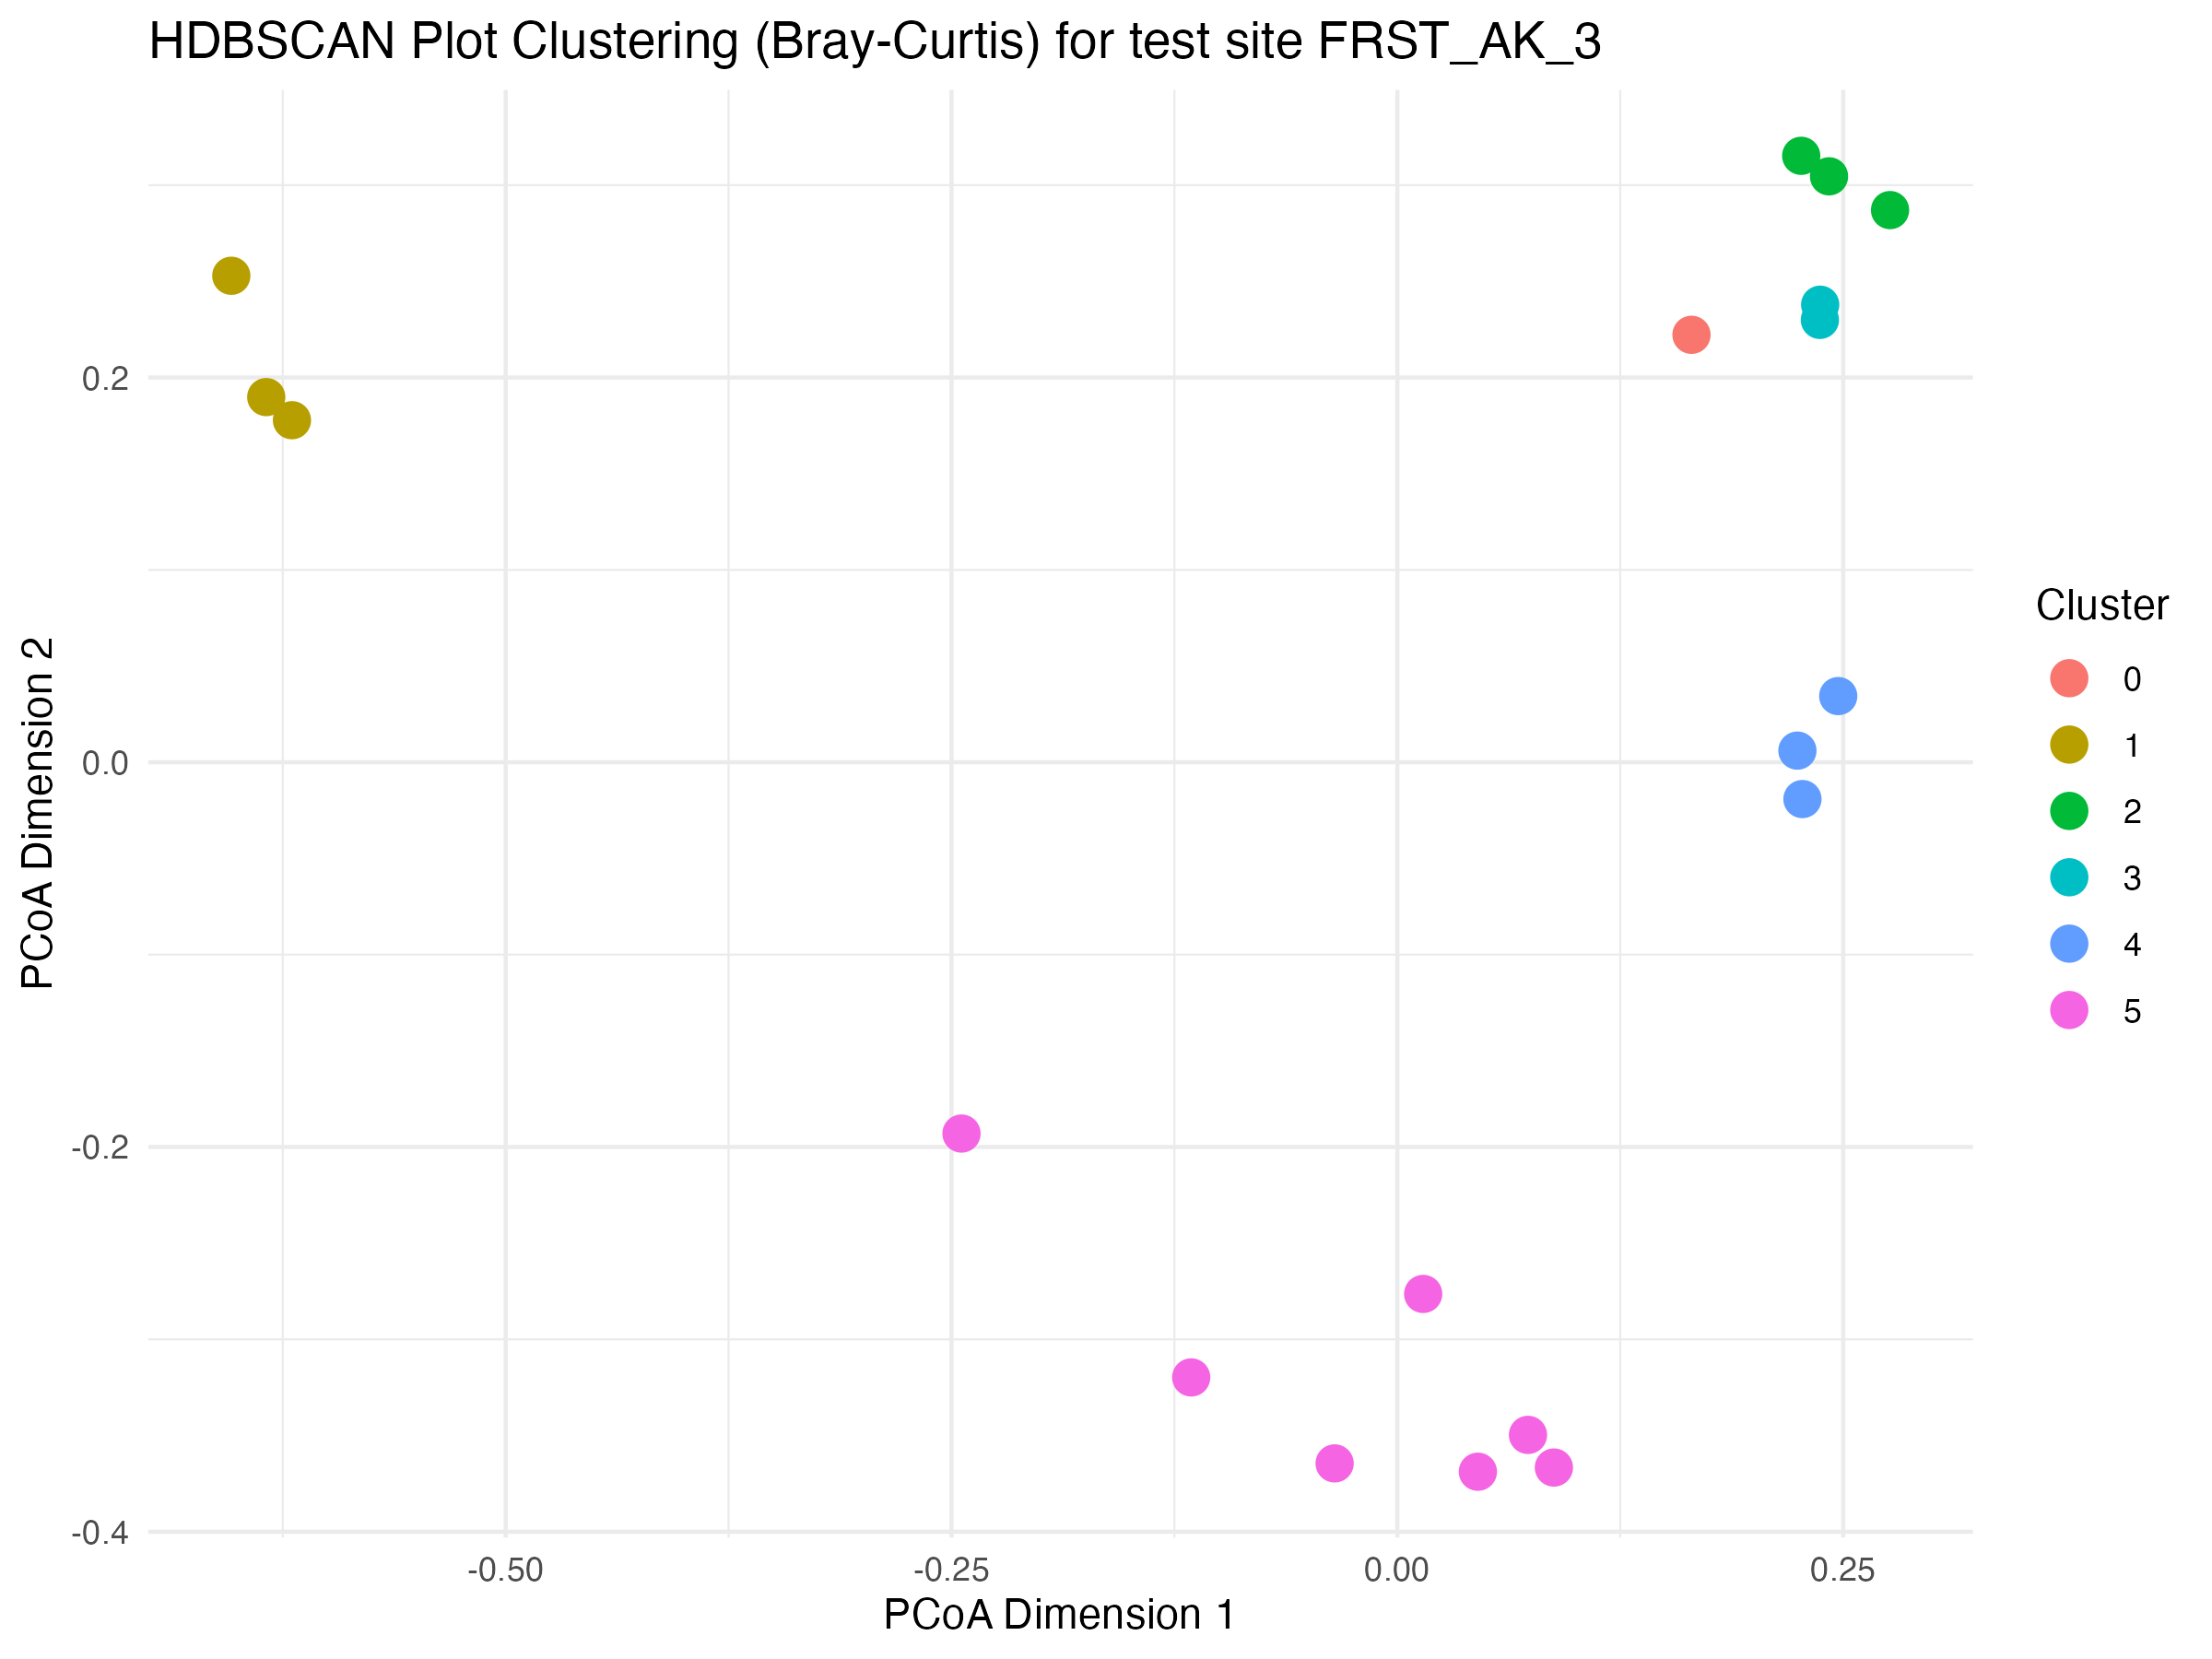
\includegraphics[width=0.9\textwidth]{Figures/Appendix/PlantCommunityClustering/FRST_AK_3_HDBSCAN_clusters.png} % Replace with your actual image path
    \caption{Community cluster HDBSCAN plot for test site FRST\_AK\_3}
    \label{fig:FRST_AK_3_HDBSCAN_clusters}
\end{figure}

\begin{figure}[H]
    \centering
    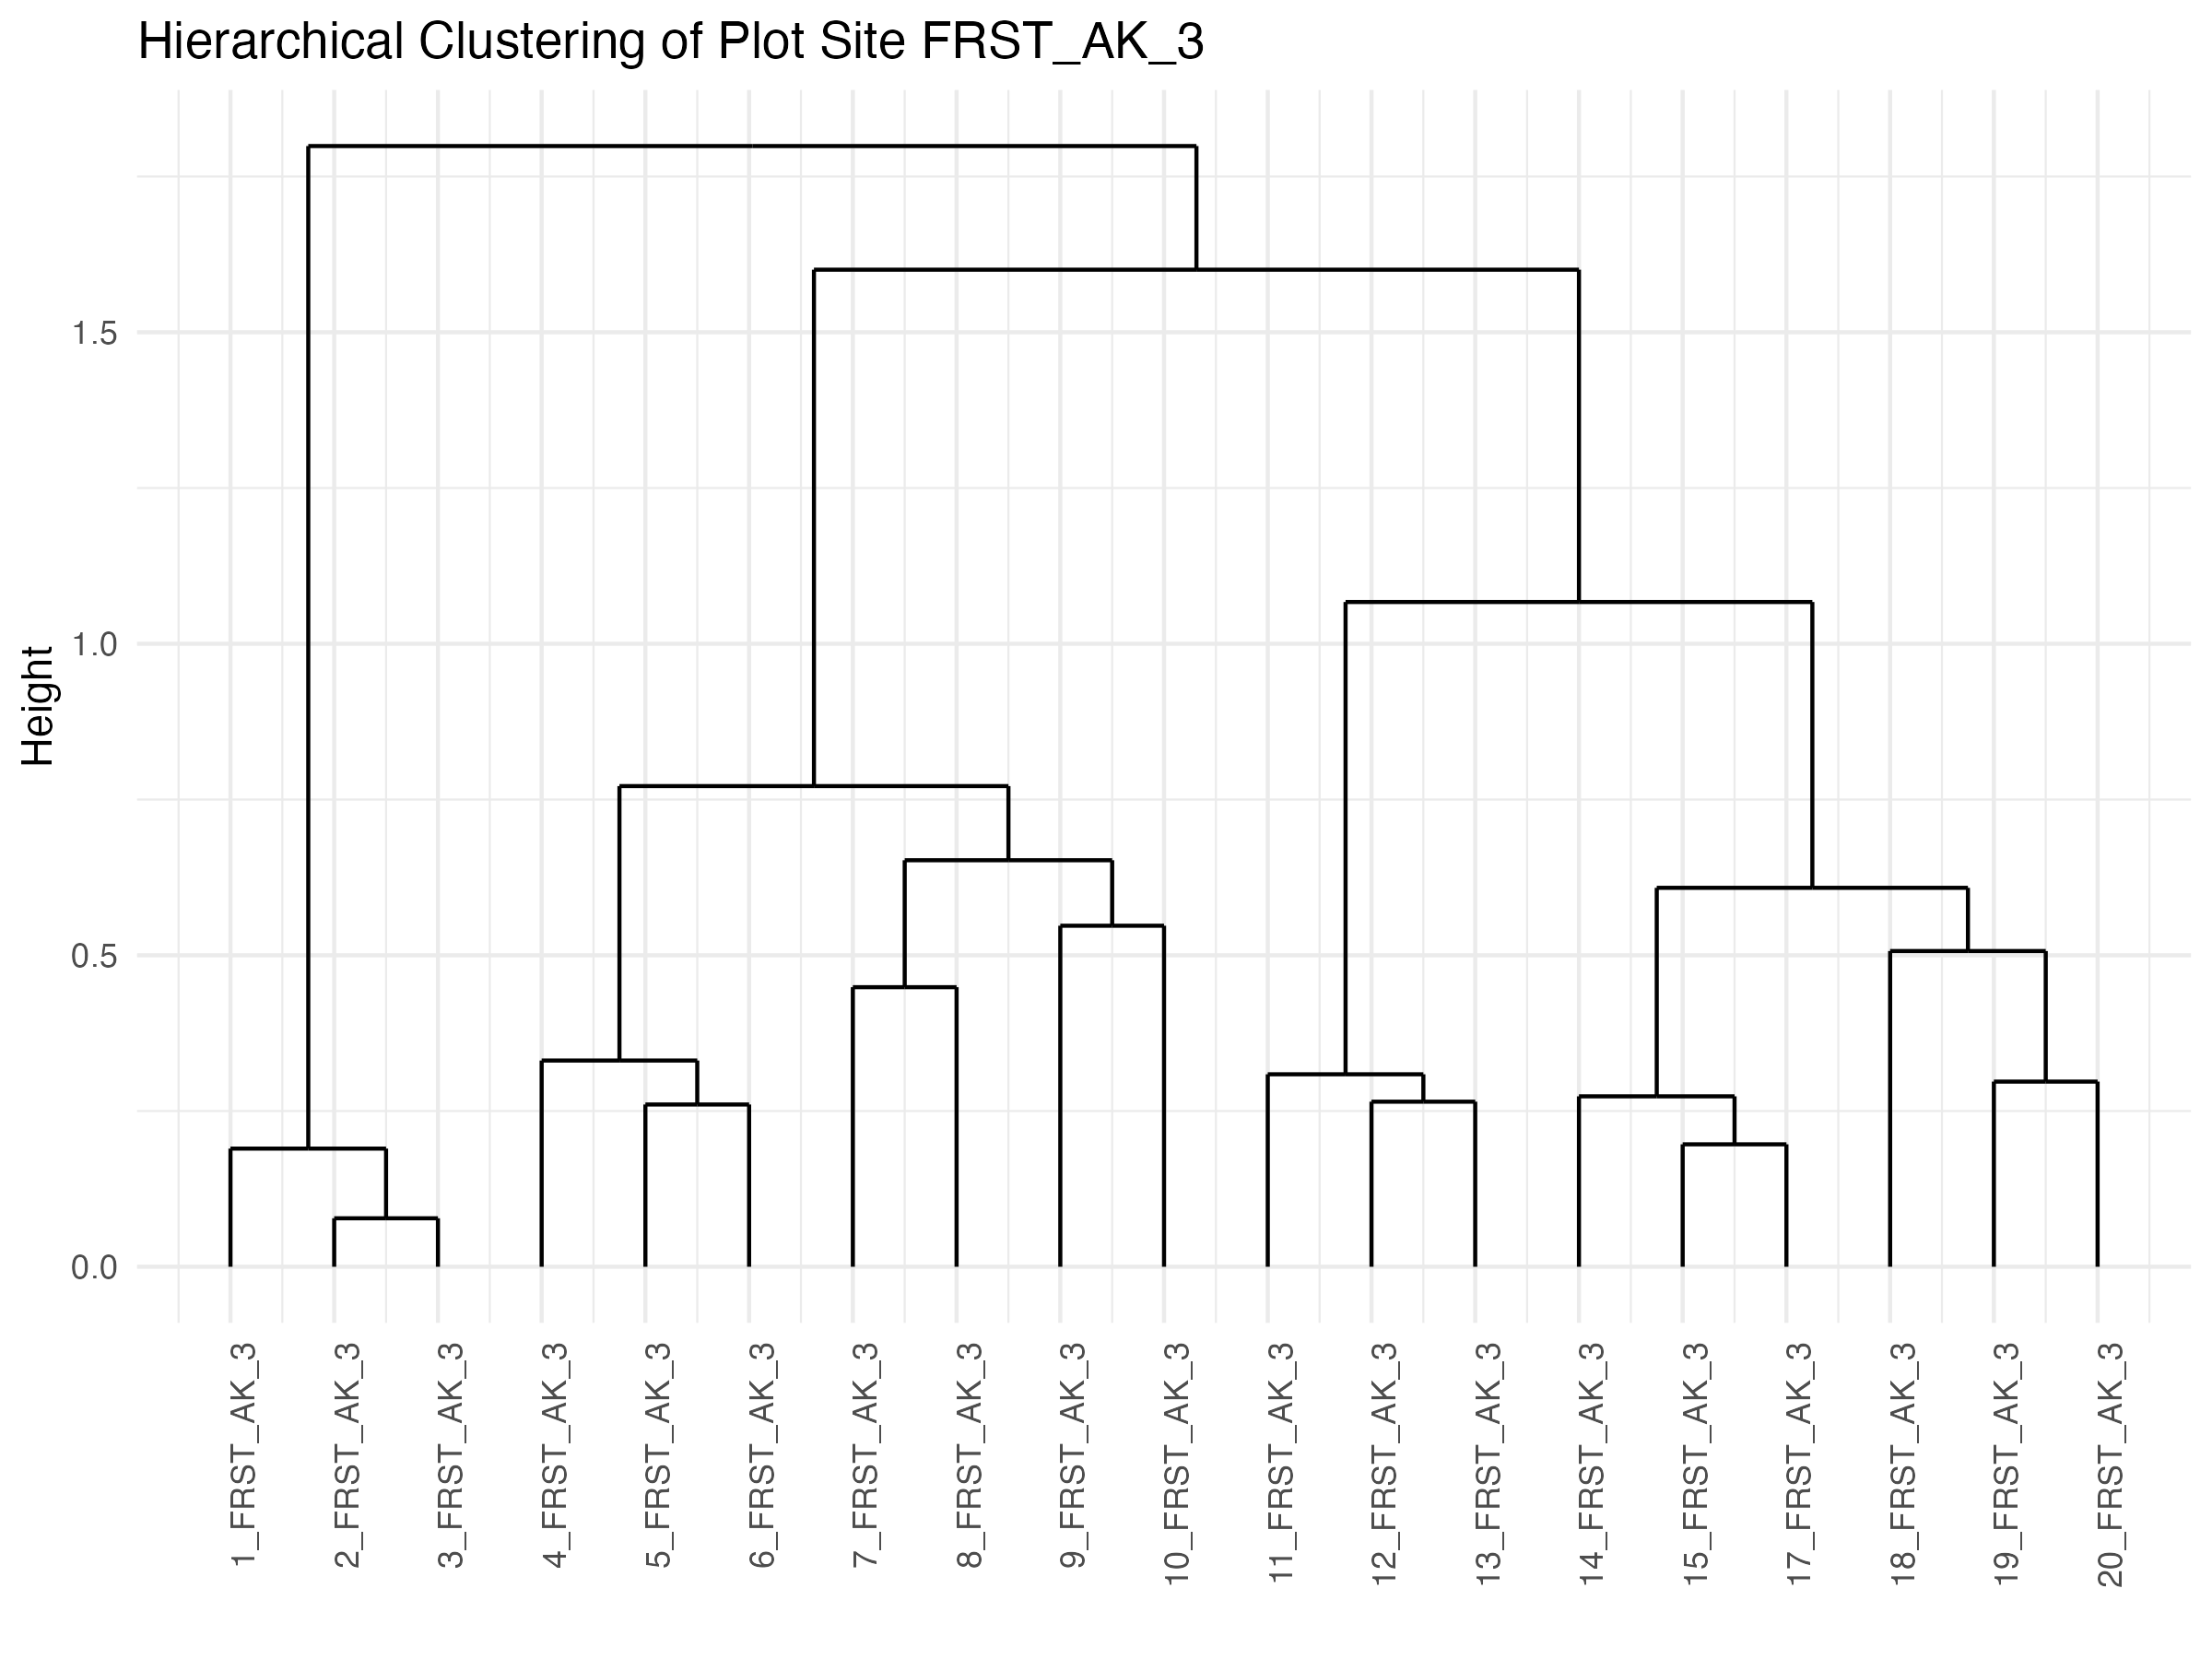
\includegraphics[width=0.9\textwidth]{Figures/Appendix/PlantCommunityClustering/FRST_AK_3_DENDRO.png} % Replace with your actual image path
    \caption{Community cluster dendrogram plot for test site FRST\_AK\_3}
    \label{fig:FRST_AK_3_DENDRO}
\end{figure}

\subsection{PRUAIR\_DW\_1}
\begin{figure}[H]
    \centering
    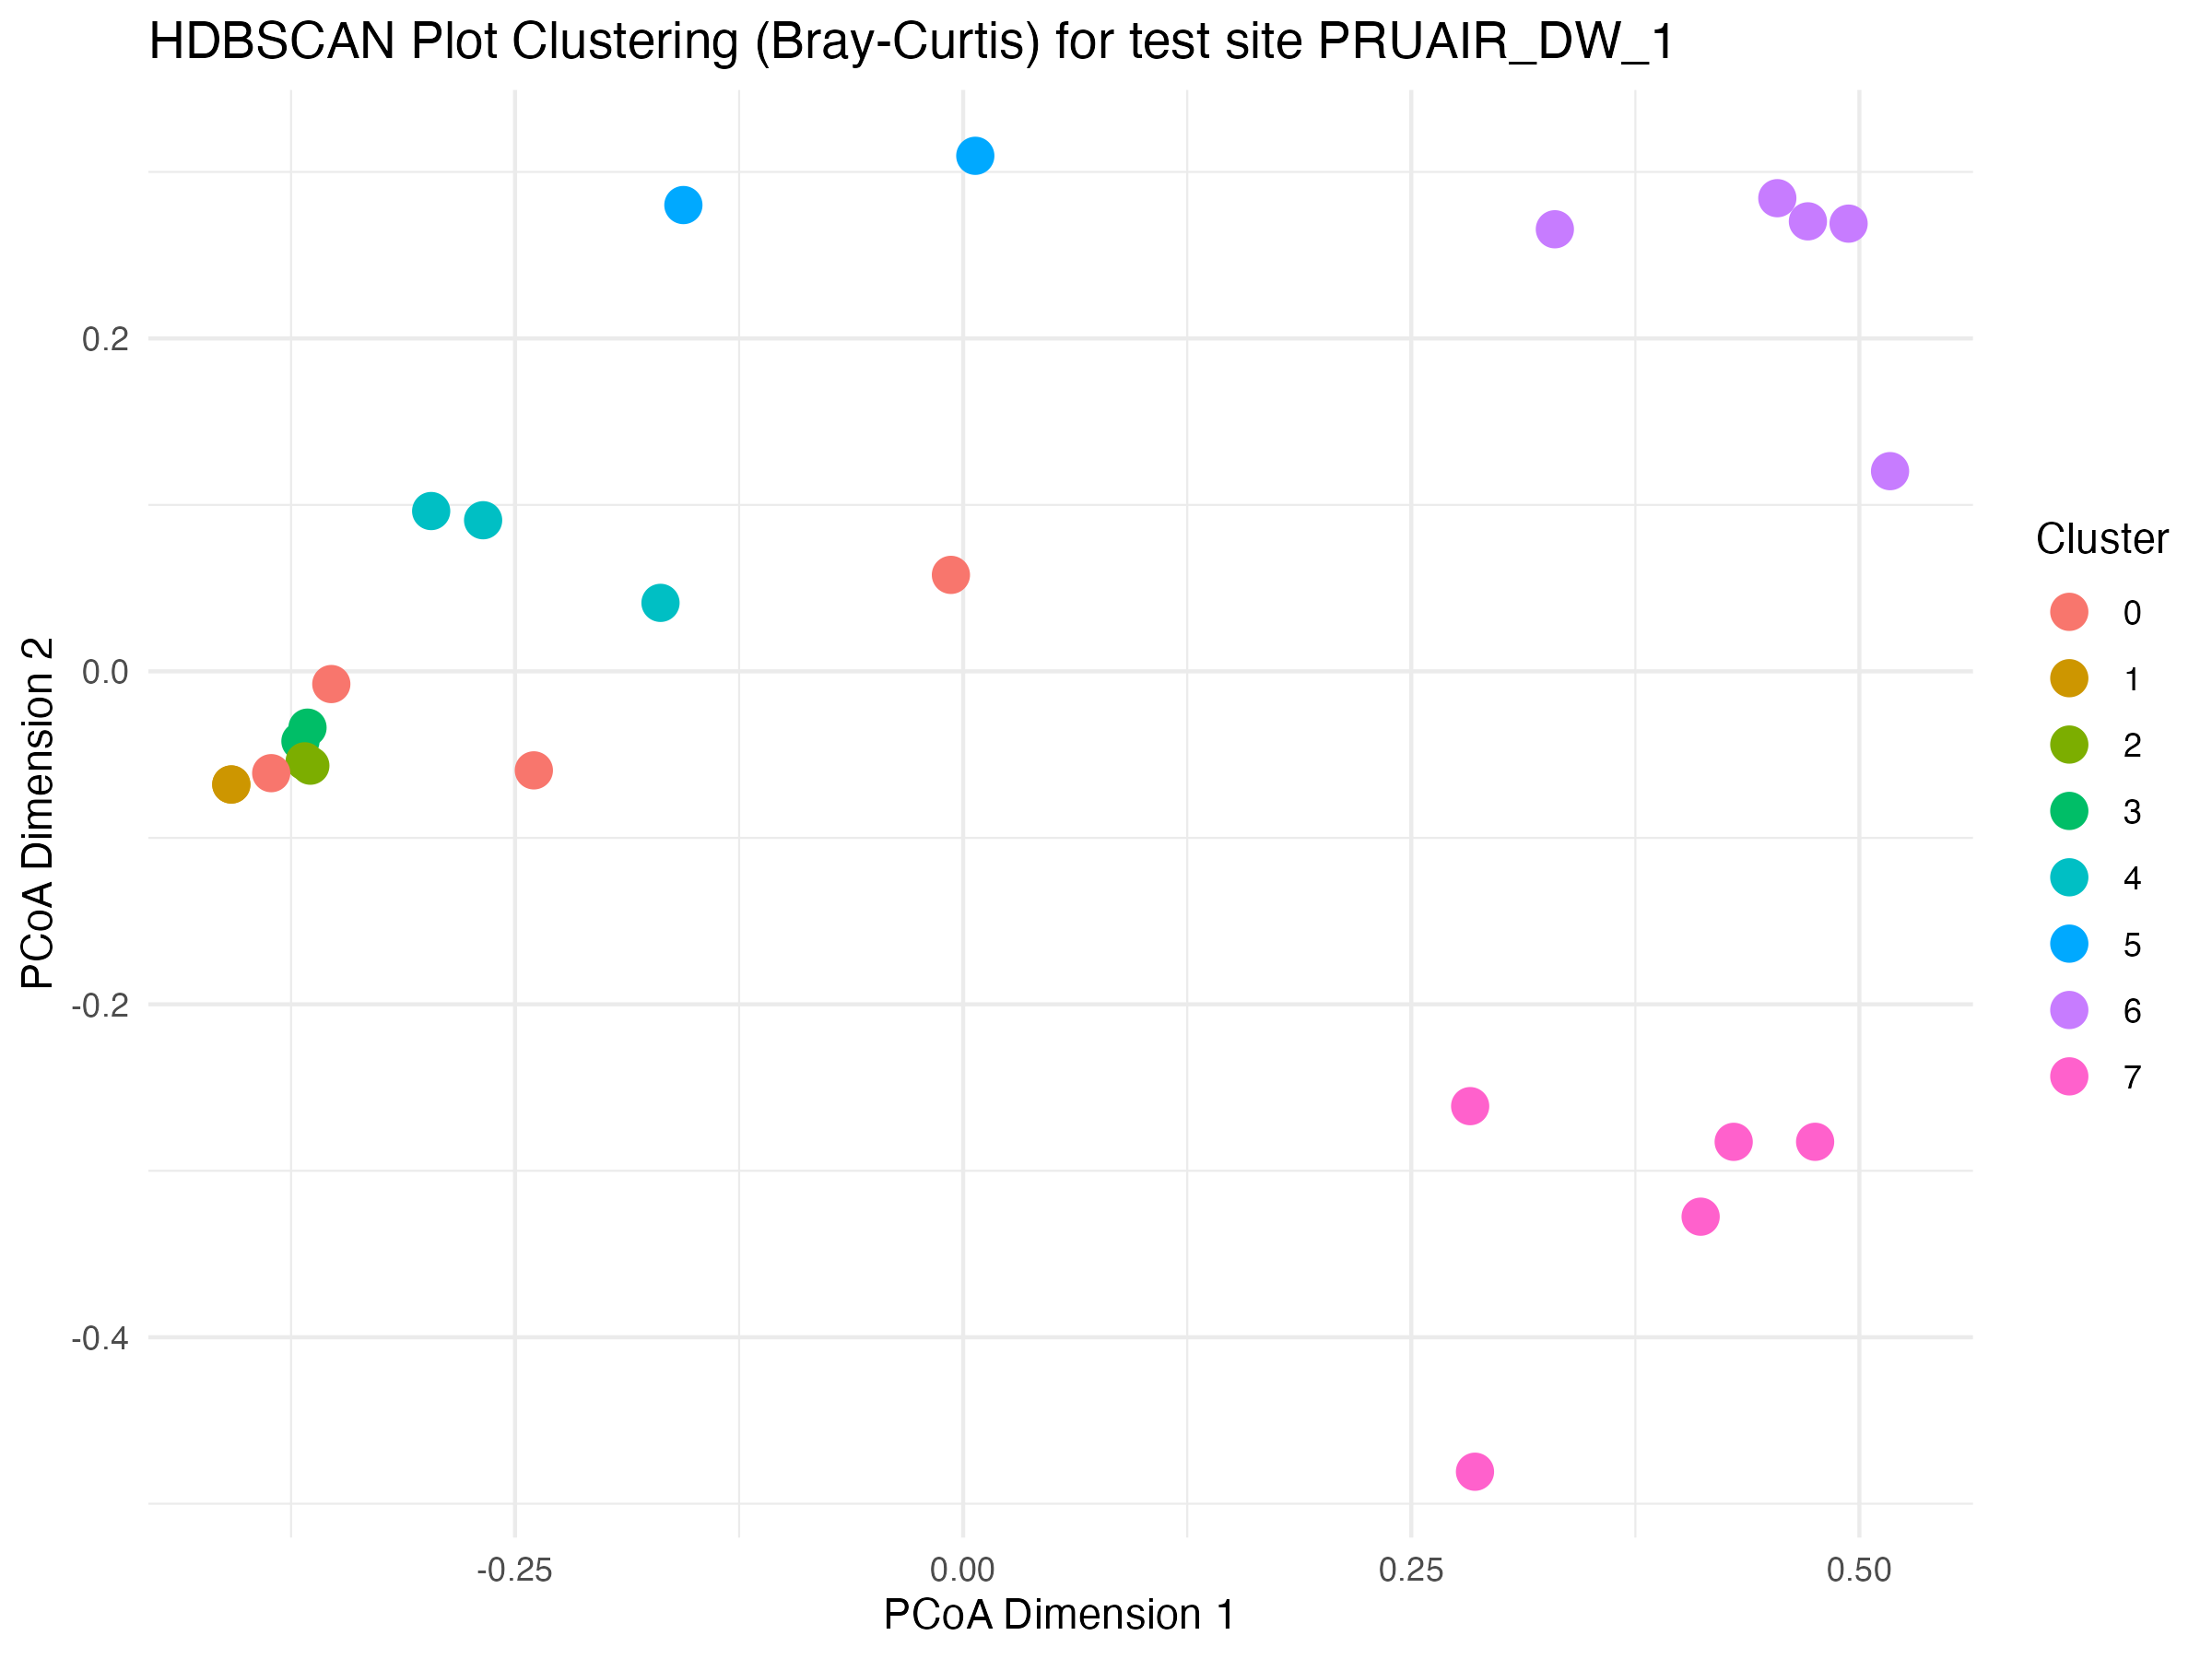
\includegraphics[width=0.9\textwidth]{Figures/Appendix/PlantCommunityClustering/PRUAIR_DW_1_HDBSCAN_clusters.png} % Replace with your actual image path
    \caption{Community cluster HDBSCAN plot for test site PRUAIR\_DW\_1}
    \label{fig:PRUAIR_DW_1_HDBSCAN_clusters}
\end{figure}

\begin{figure}[H]
    \centering
    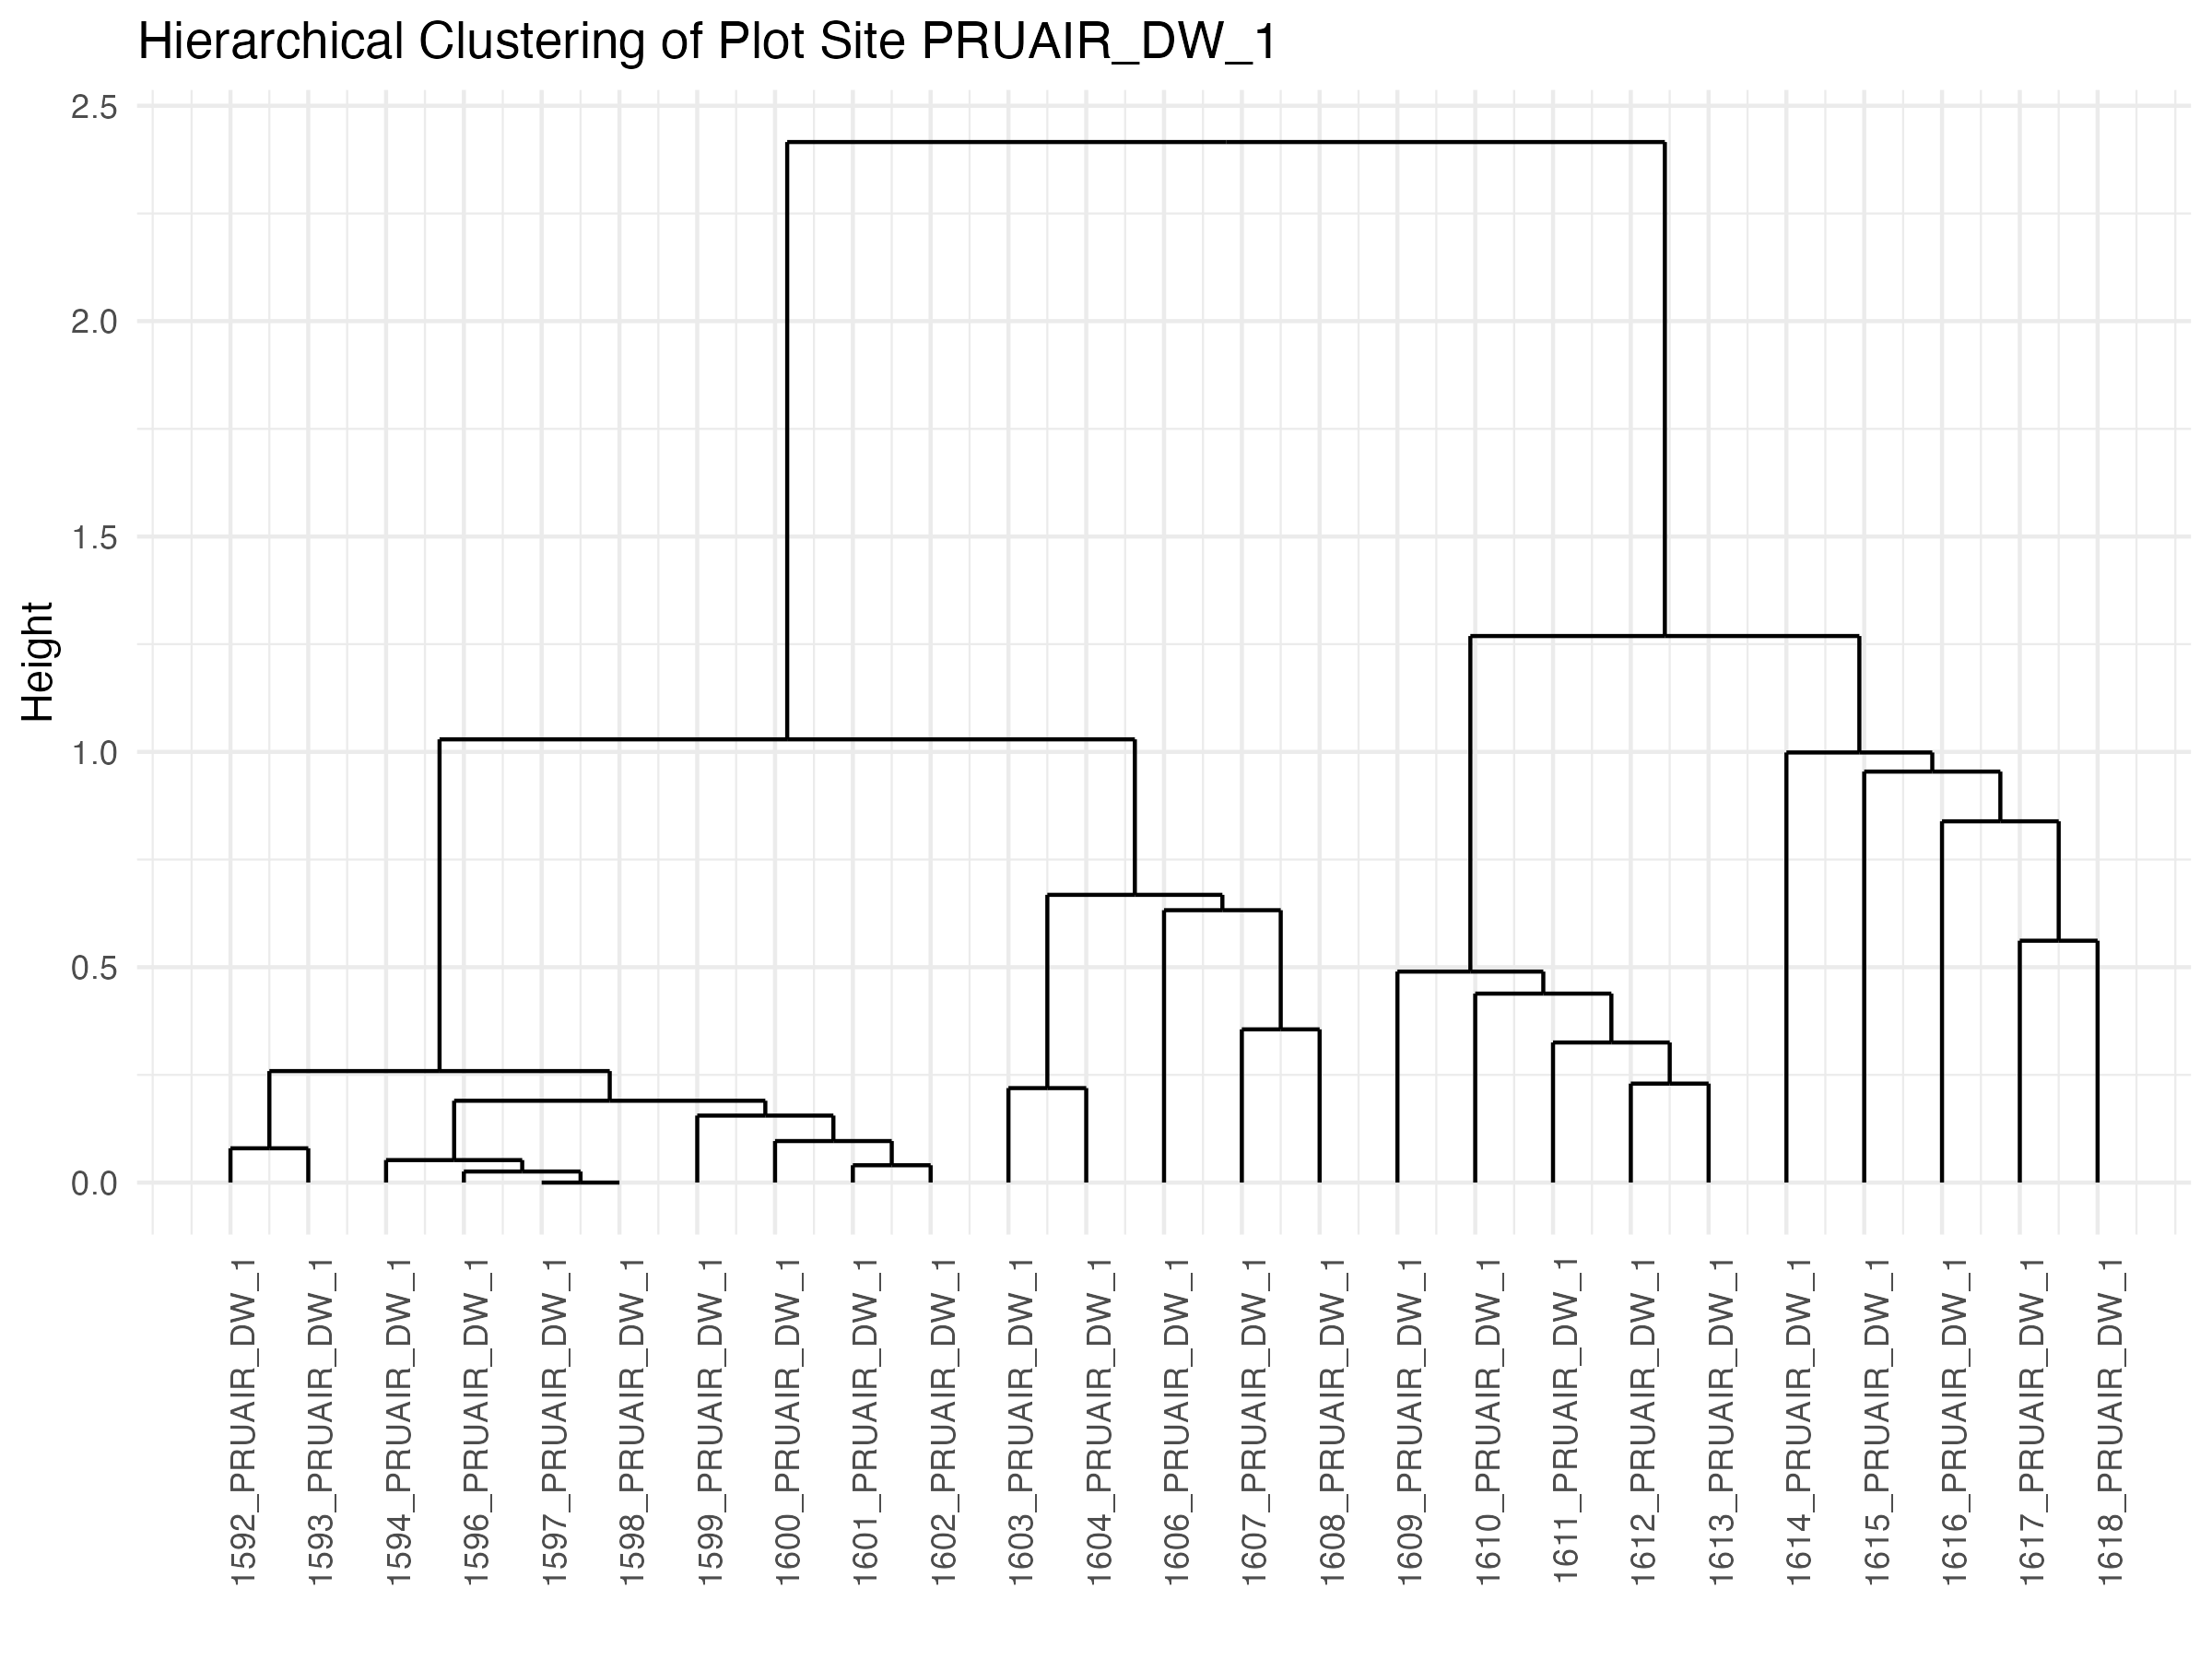
\includegraphics[width=0.9\textwidth]{Figures/Appendix/PlantCommunityClustering/PRUAIR_DW_1_DENDRO.png} % Replace with your actual image path
    \caption{Community cluster dendrogram plot for test site PRUAIR\_DW\_1}
    \label{fig:PRUAIR_DW_1_DENDRO}
\end{figure}

\subsection{PRUARC\_DW\_1}
\begin{figure}[H]
    \centering
    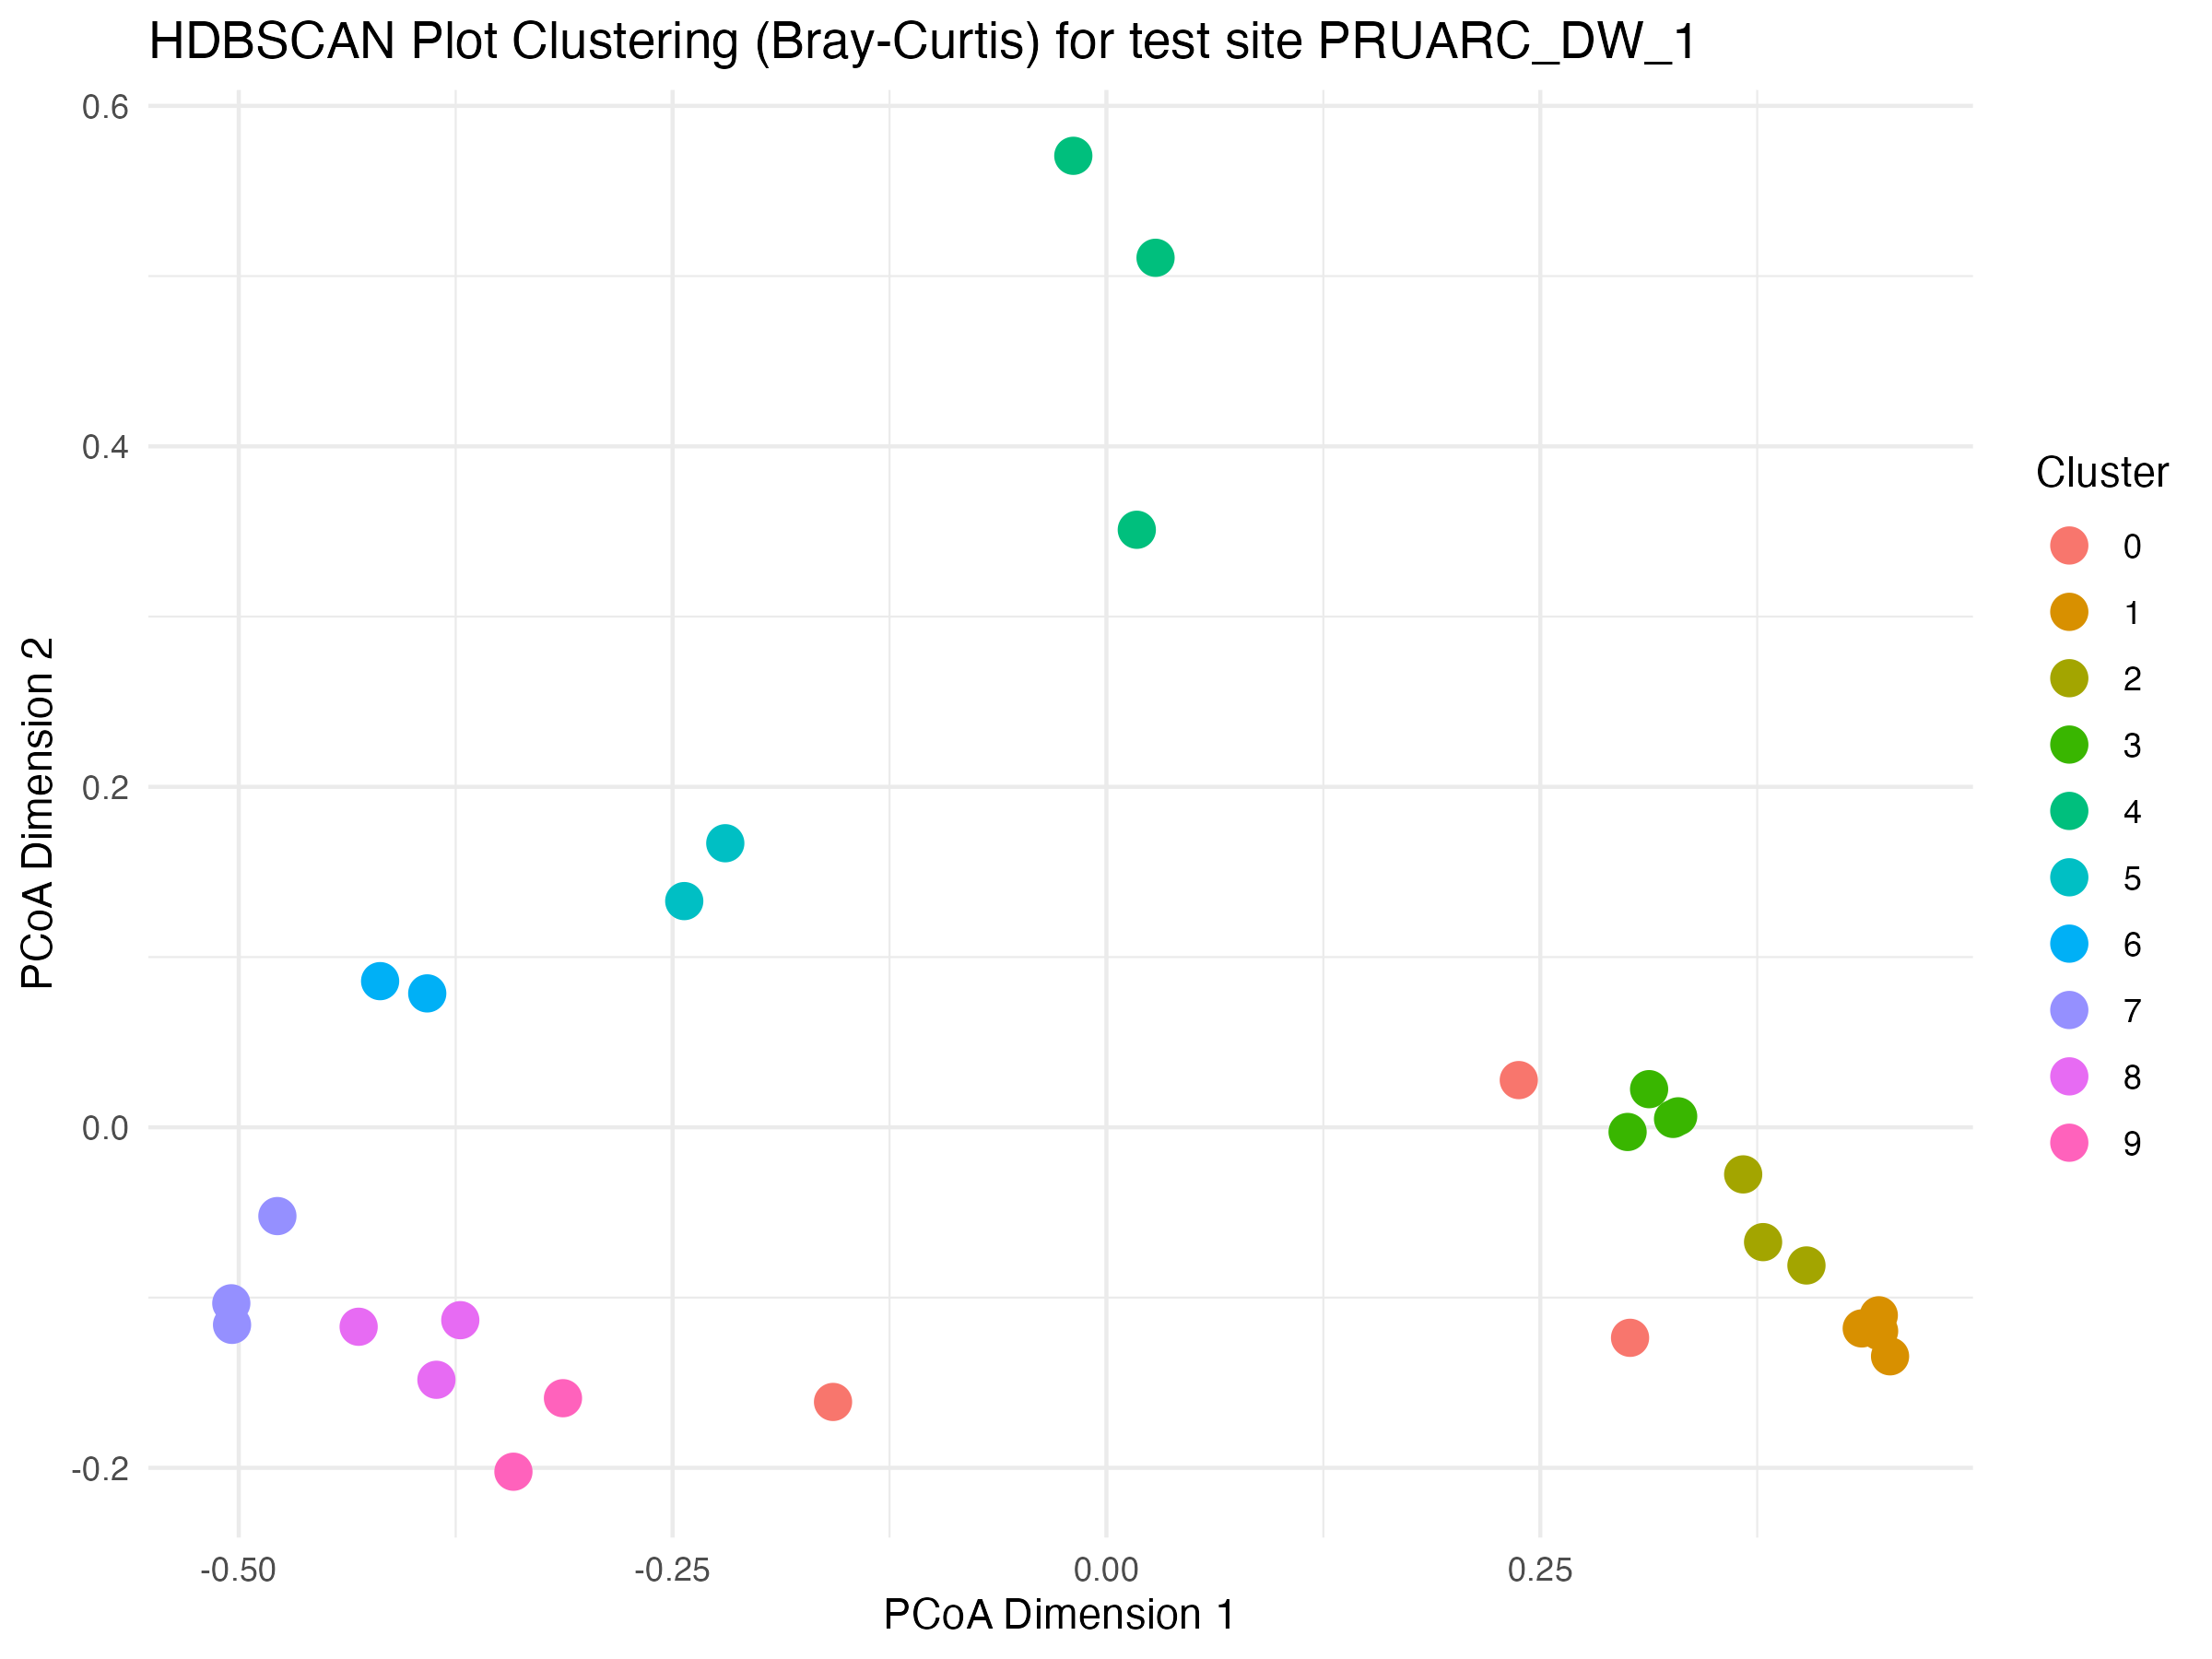
\includegraphics[width=0.9\textwidth]{Figures/Appendix/PlantCommunityClustering/PRUARC_DW_1_HDBSCAN_clusters.png} % Replace with your actual image path
    \caption{Community cluster HDBSCAN plot for test site PRUARC\_DW\_1}
    \label{fig:PRUARC_DW_1_HDBSCAN_clusters}
\end{figure}

\begin{figure}[H]
    \centering
    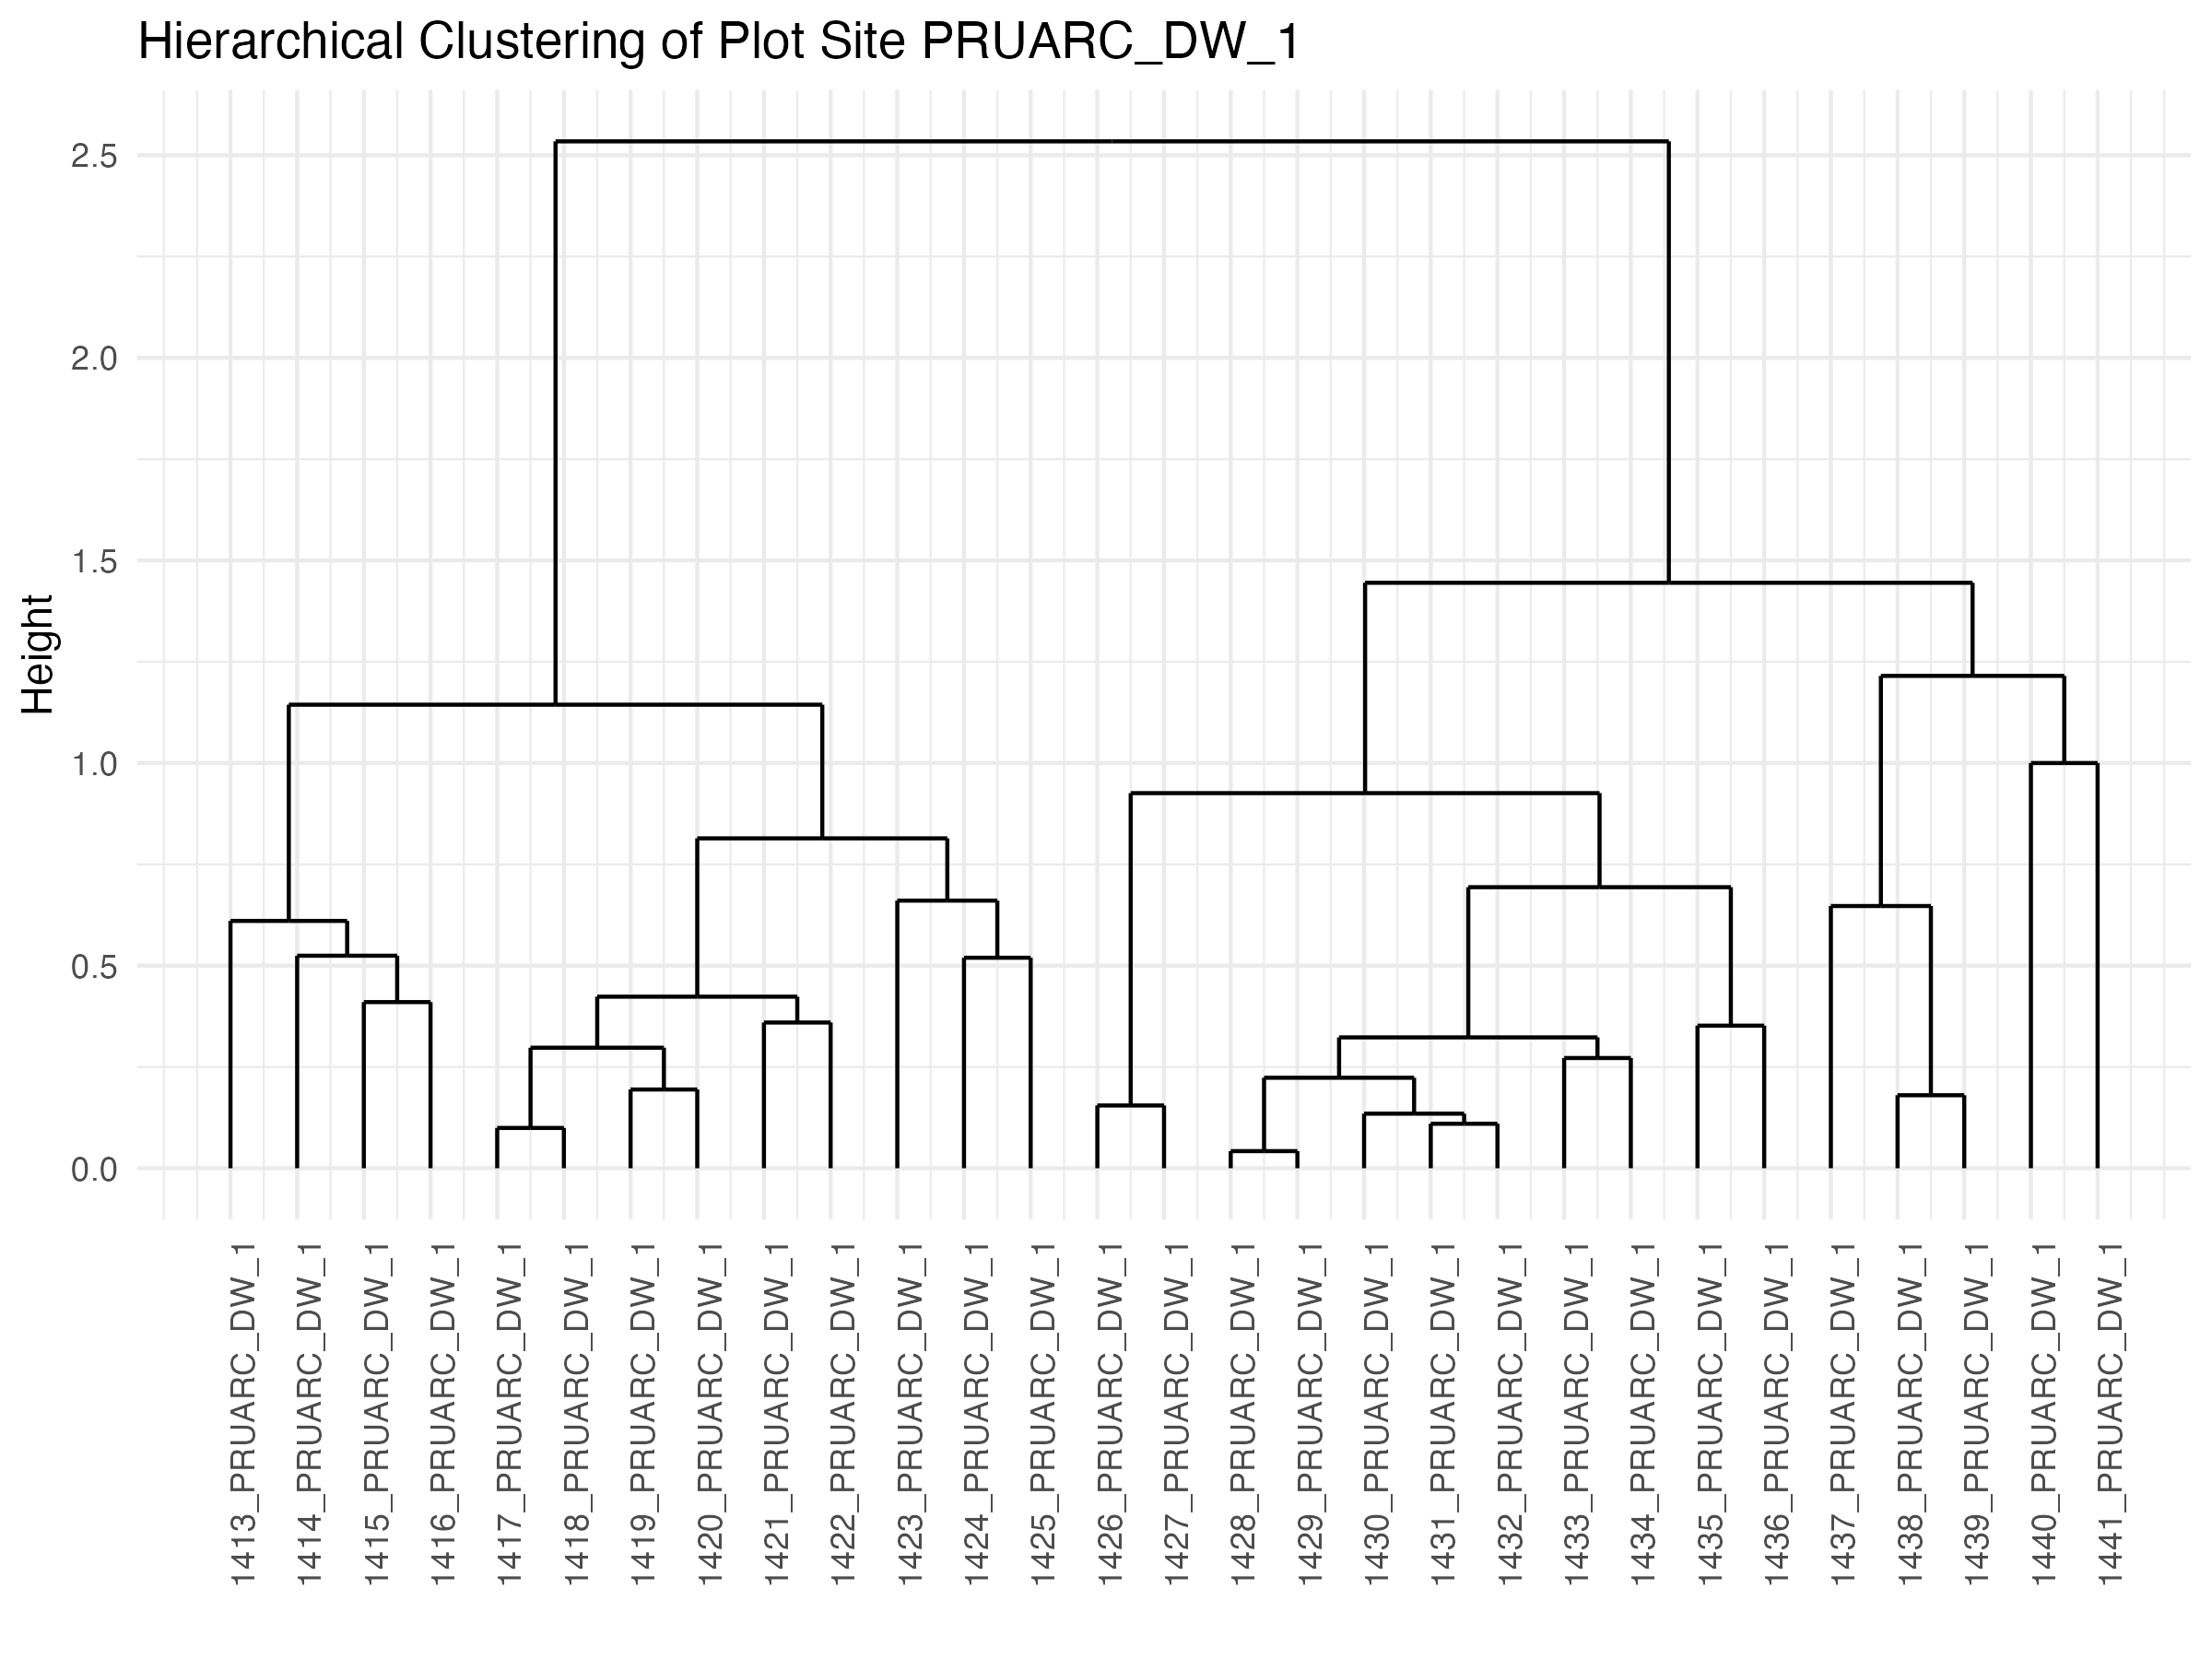
\includegraphics[width=0.9\textwidth]{Figures/Appendix/PlantCommunityClustering/PRUARC_DW_1_DENDRO.png} % Replace with your actual image path
    \caption{Community cluster dendrogram plot for test site PRUARC\_DW\_1}
    \label{fig:PRUARC_DW_1_DENDRO}
\end{figure}





% \subsection{Hugo}
% % Group 1 of 4
% \begin{figure}[H]
%     \centering
%     \begin{minipage}[b]{0.45\textwidth}
%         \centering
%         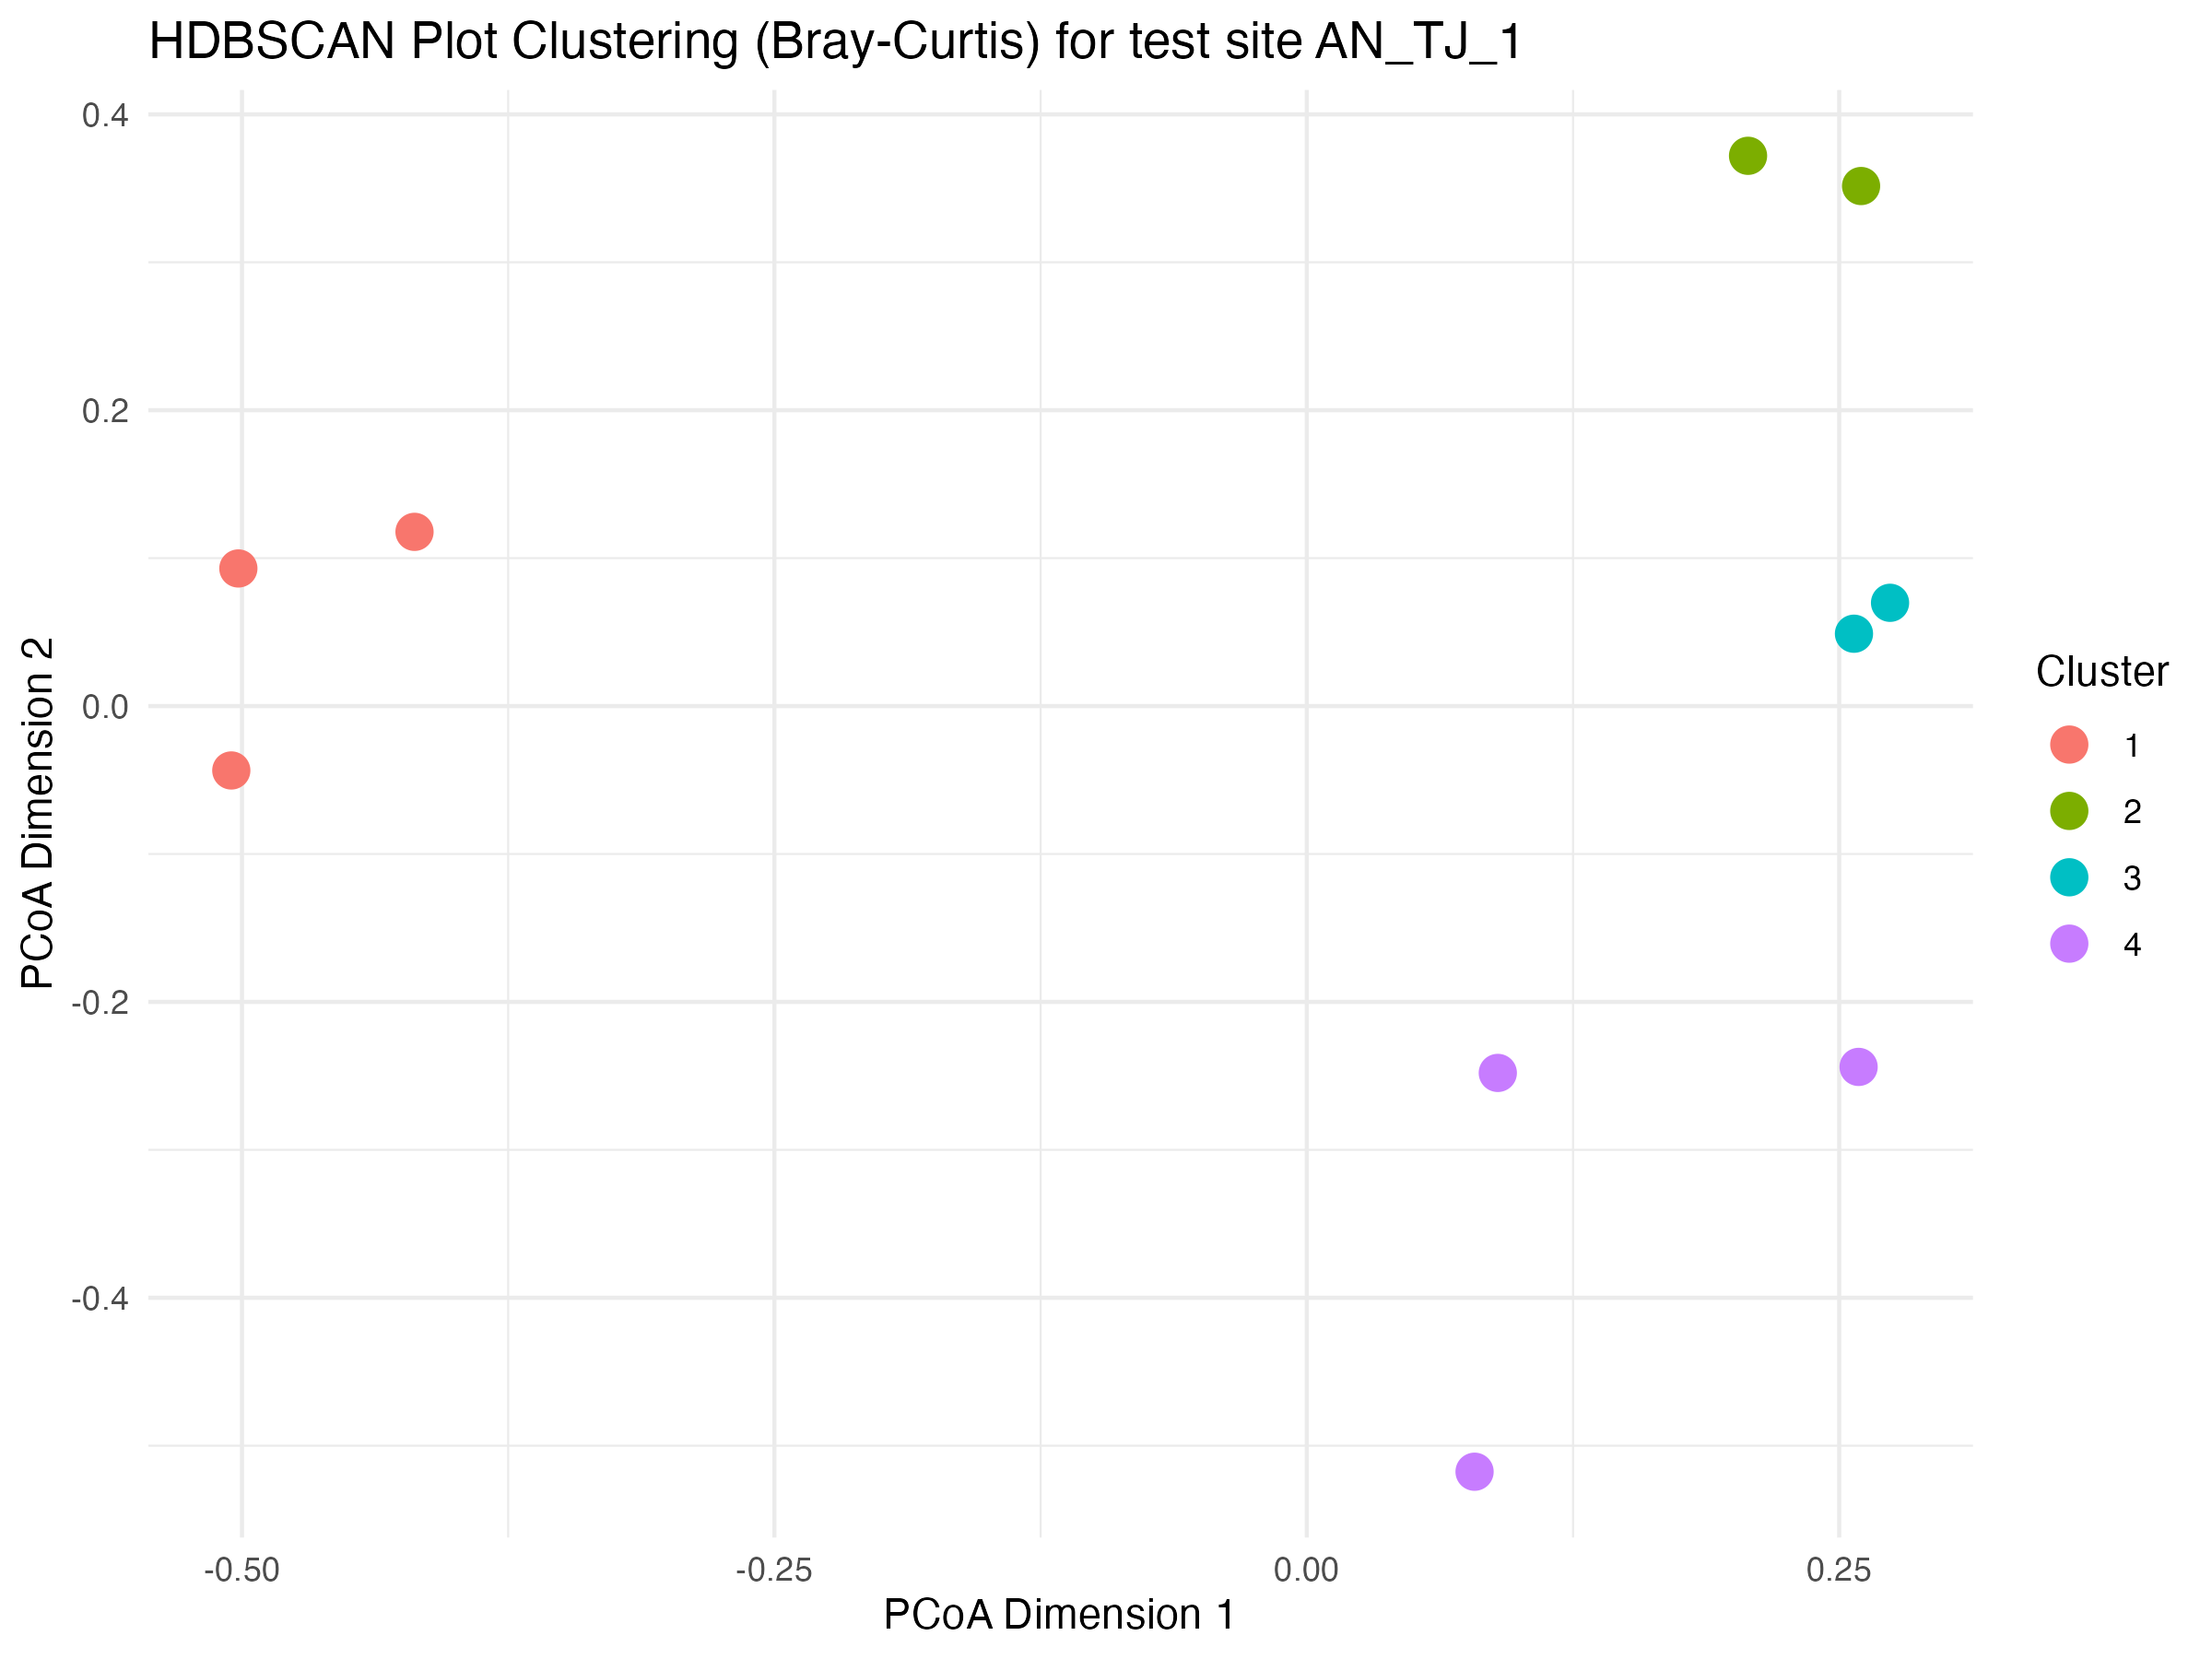
\includegraphics[width=\textwidth]{Figures/Appendix/PlantCommunityClustering/AN_TJ_1_HDBSCAN_clusters.png}
%         \caption{AN\_TJ\_1}
%         \label{fig:AN_TJ_1_HDBSCAN_clusters}
%     \end{minipage}
%     \hfill
%     \begin{minipage}[b]{0.45\textwidth}
%         \centering
%         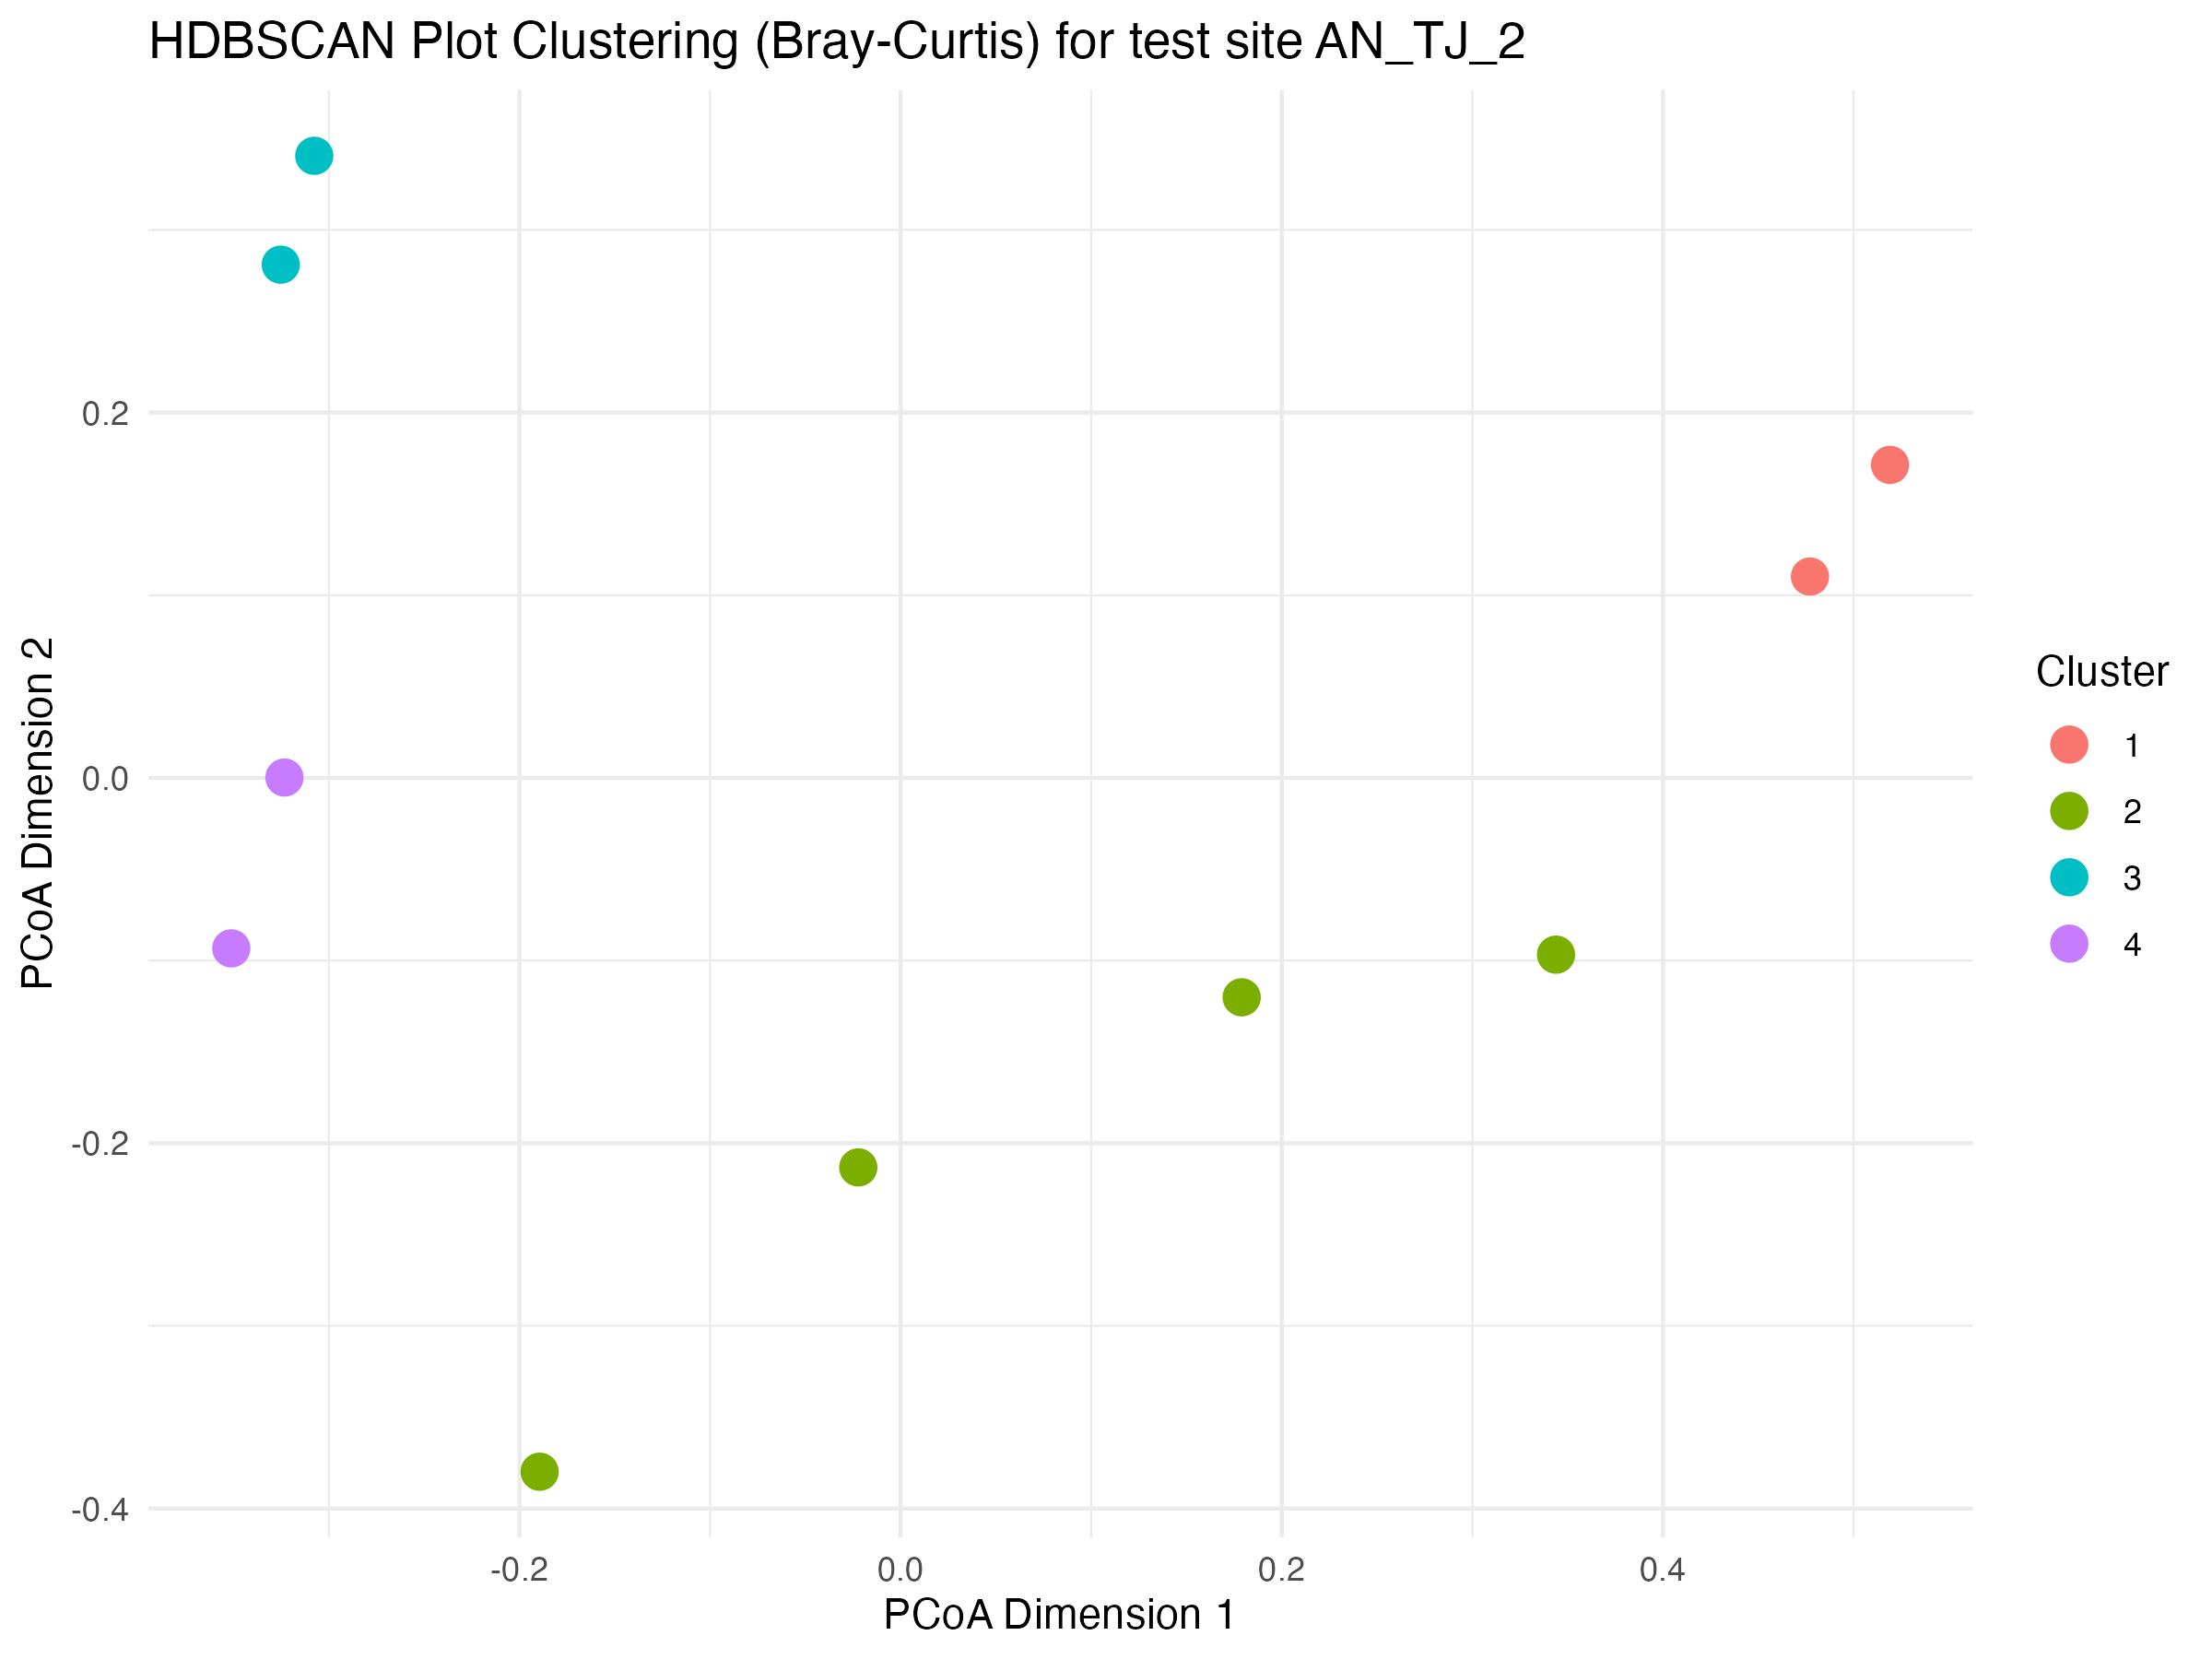
\includegraphics[width=\textwidth]{Figures/Appendix/PlantCommunityClustering/AN_TJ_2_HDBSCAN_clusters.png}
%         \caption{AN\_TJ\_2}
%         \label{fig:AN_TJ_2_HDBSCAN_clusters}
%     \end{minipage}

%     \vspace{1cm} % Space between rows of images

%     \begin{minipage}[b]{0.45\textwidth}
%         \centering
%         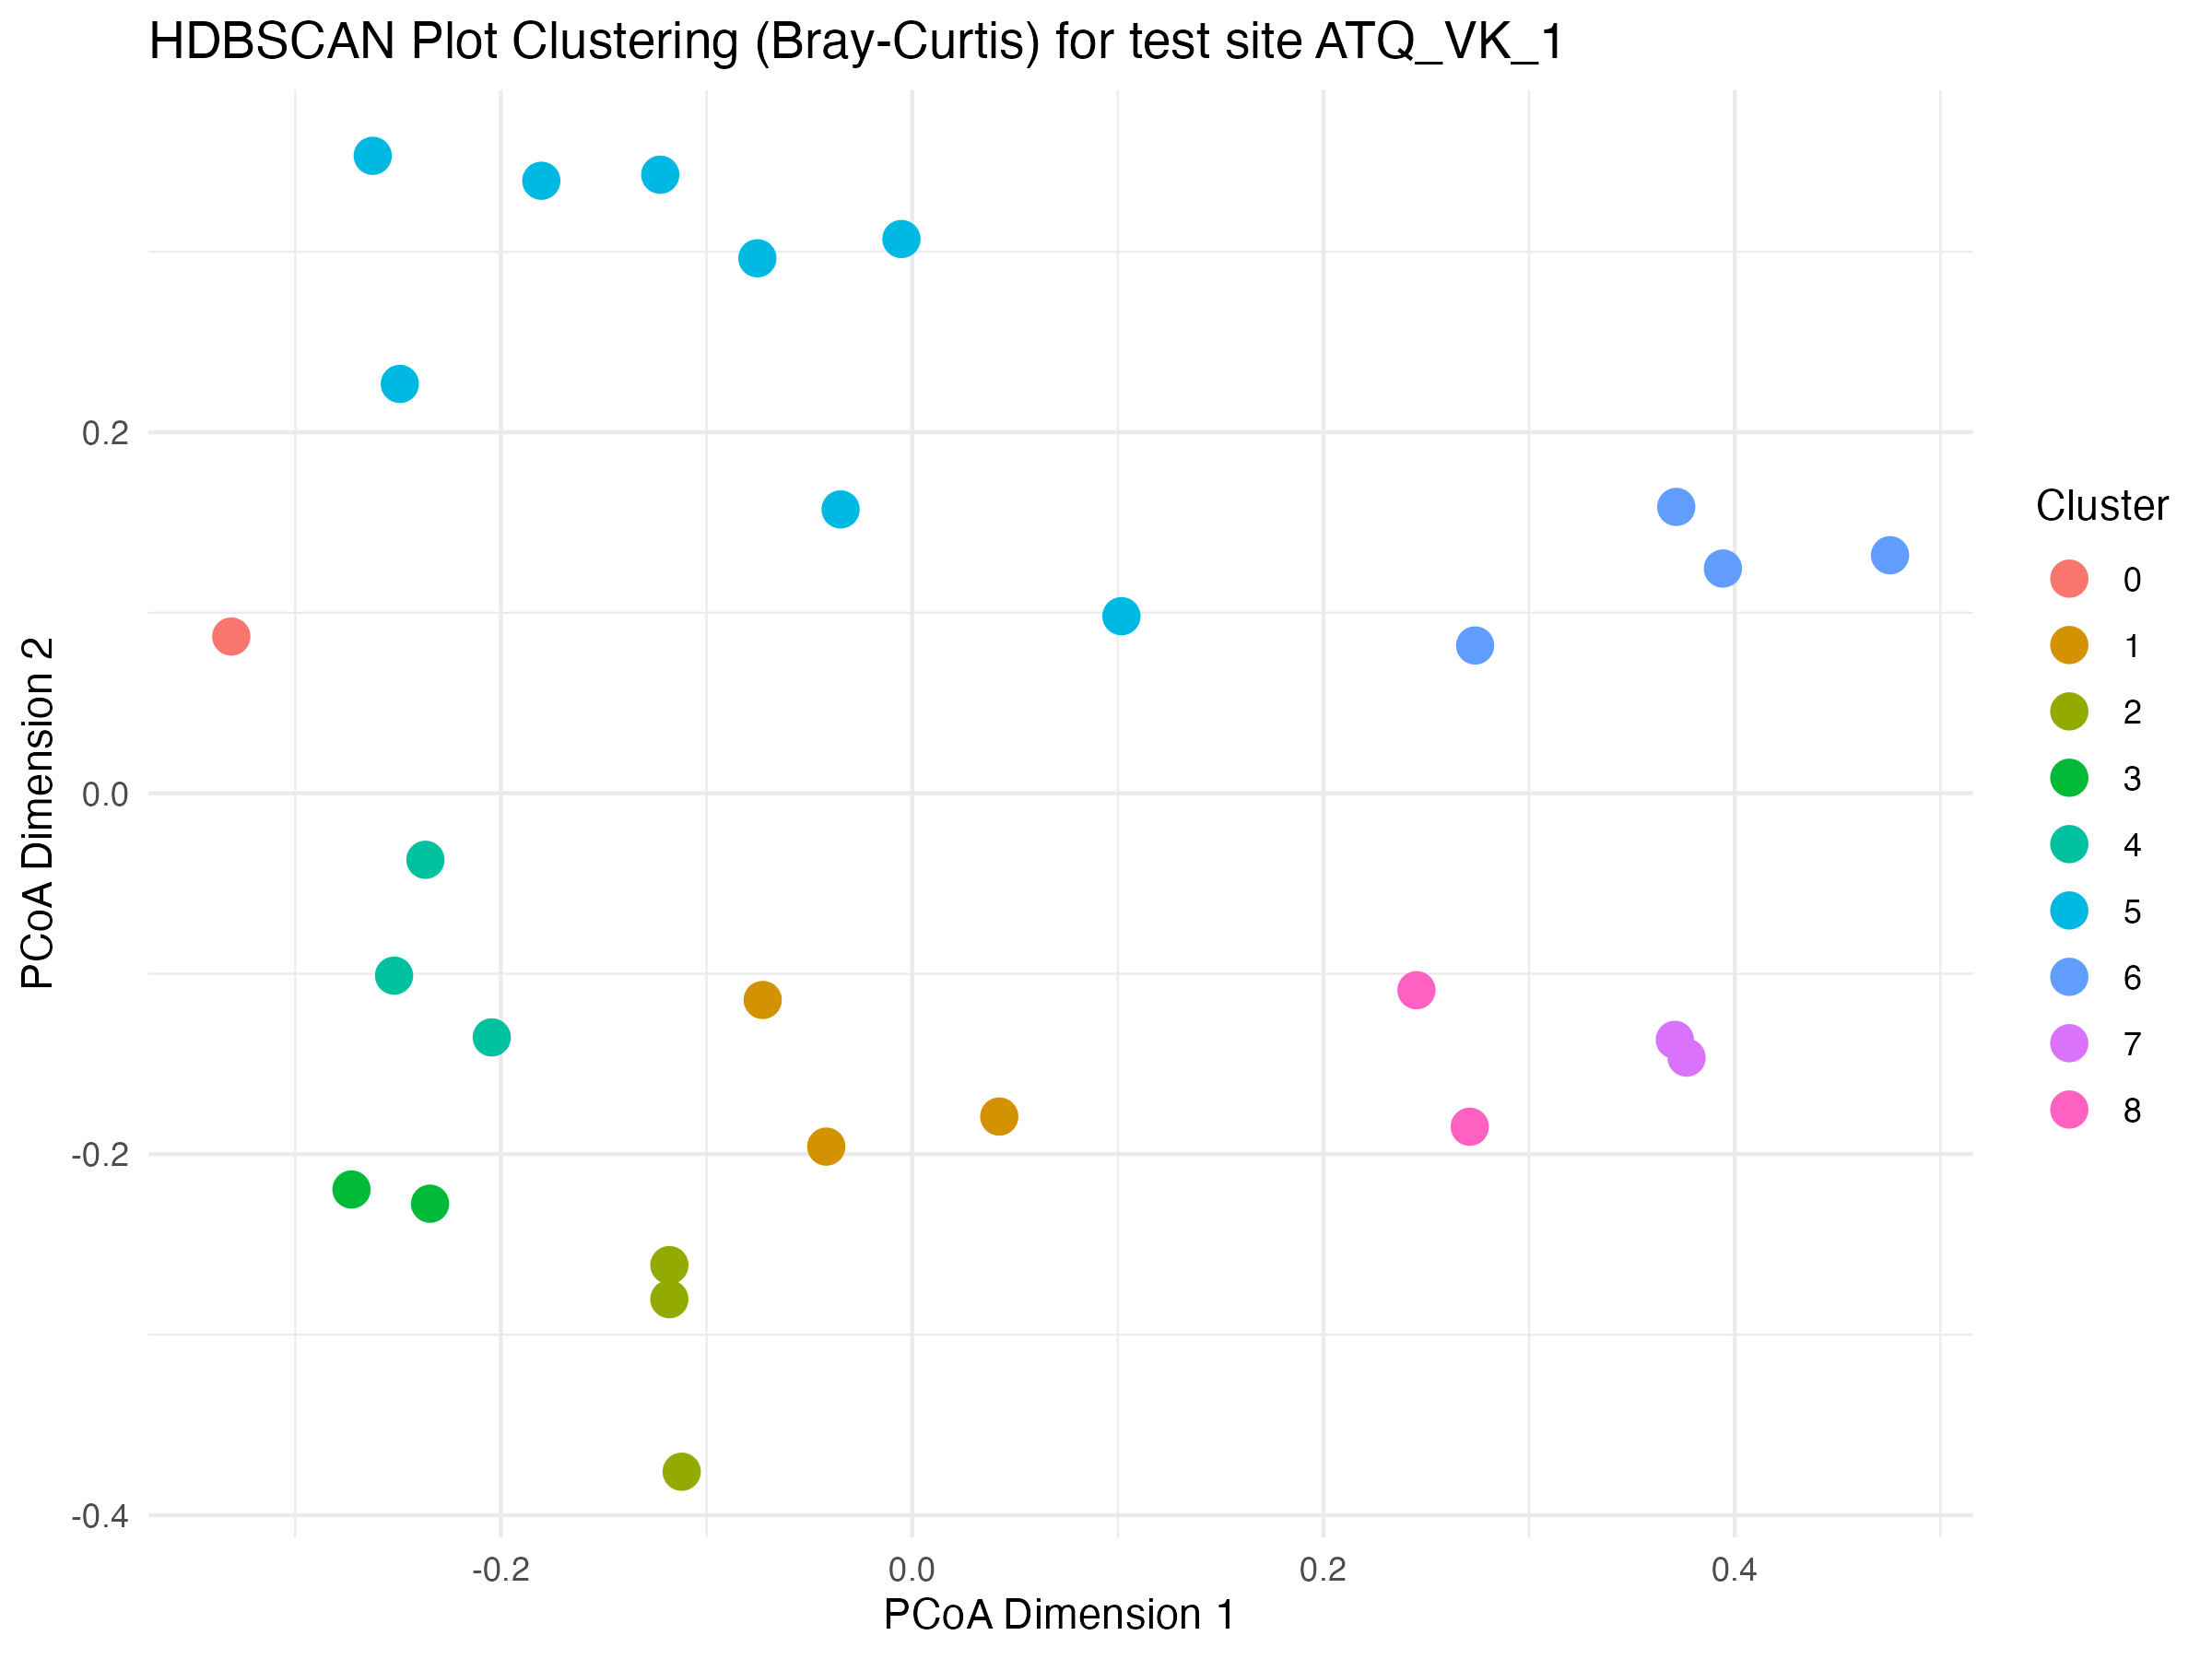
\includegraphics[width=\textwidth]{Figures/Appendix/PlantCommunityClustering/ATQ_VK_1_HDBSCAN_clusters.png}
%         \caption{ATQ\_VK\_1}
%         \label{fig:ATQ_VK_1_HDBSCAN_clusters}
%     \end{minipage}
%     \hfill
%     \begin{minipage}[b]{0.45\textwidth}
%         \centering
%         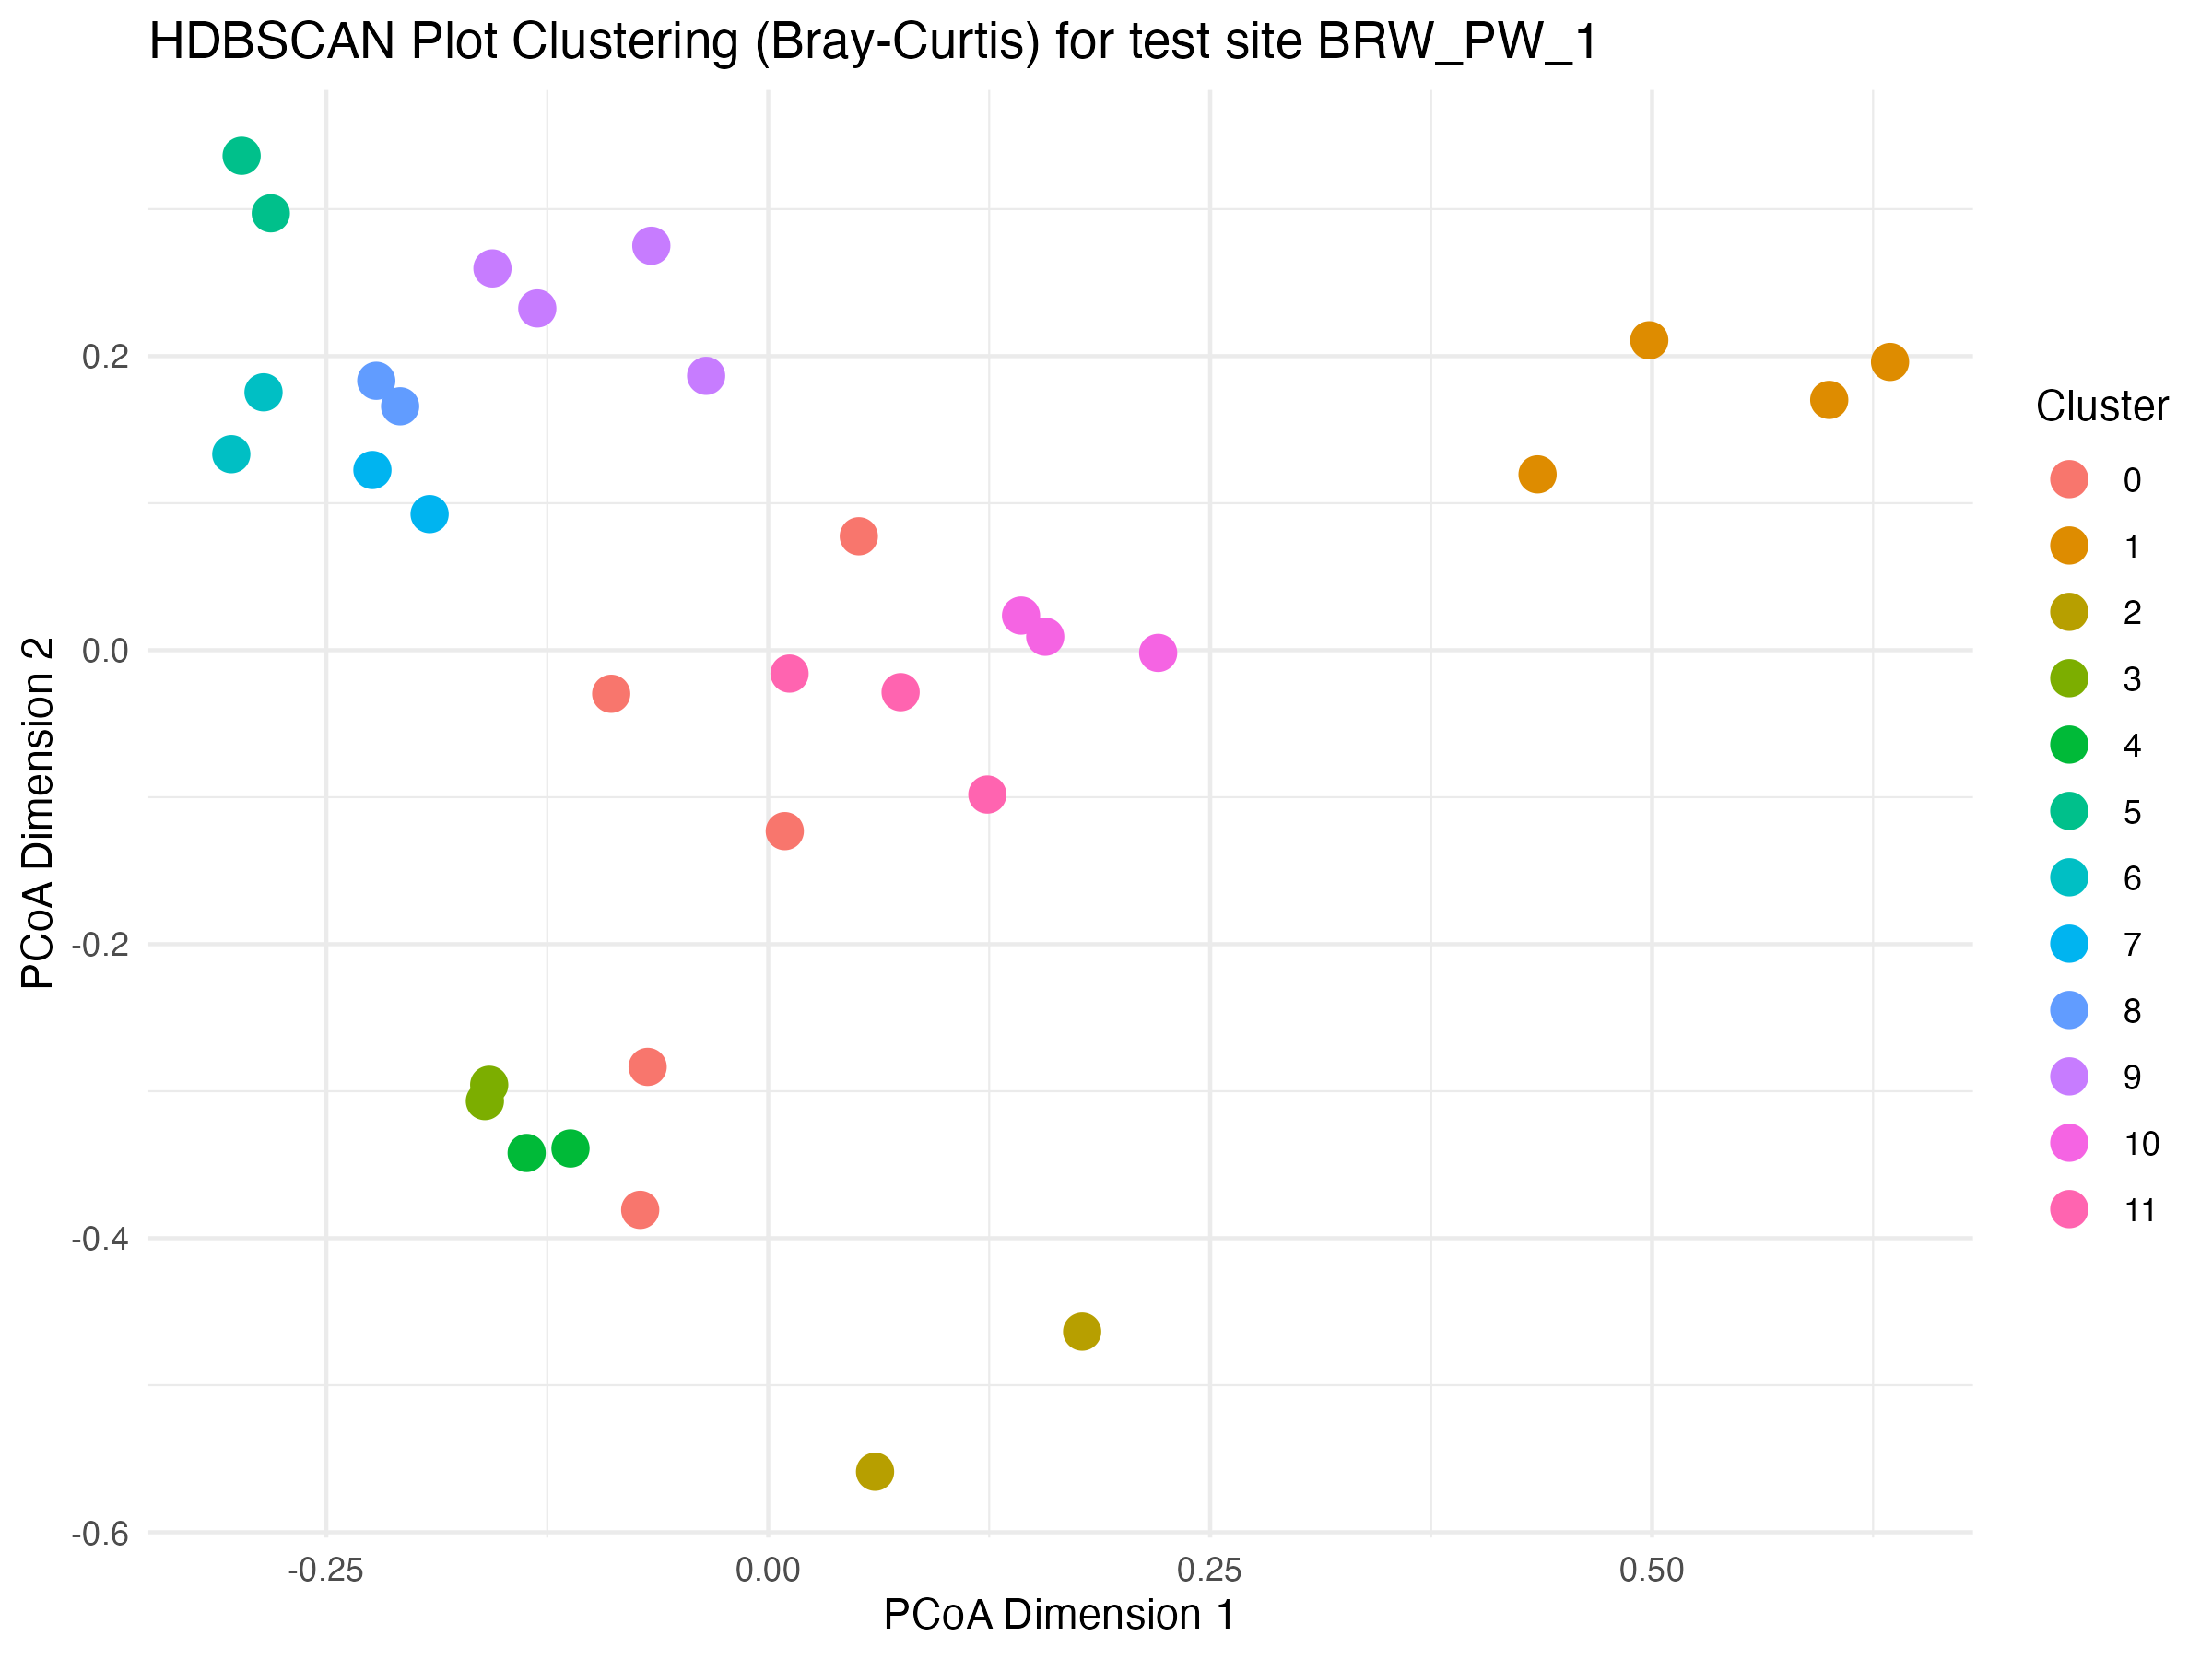
\includegraphics[width=\textwidth]{Figures/Appendix/PlantCommunityClustering/BRW_PW_1_HDBSCAN_clusters.png}
%         \caption{BRW\_PW\_1}
%         \label{fig:BRW_PW_1_HDBSCAN_clusters}
%     \end{minipage}
%     \captionof{figure}{Community Cluster Plots for Test Sites AN\_TJ\_1, AN\_TJ\_2, ATQ\_VK\_1, and BRW\_PW\_1}
%     \label{fig:group1_clusters}
% \end{figure}

% % Group 2 of 4
% \begin{figure}[H]
%     \centering
%     \begin{minipage}[b]{0.45\textwidth}
%         \centering
%         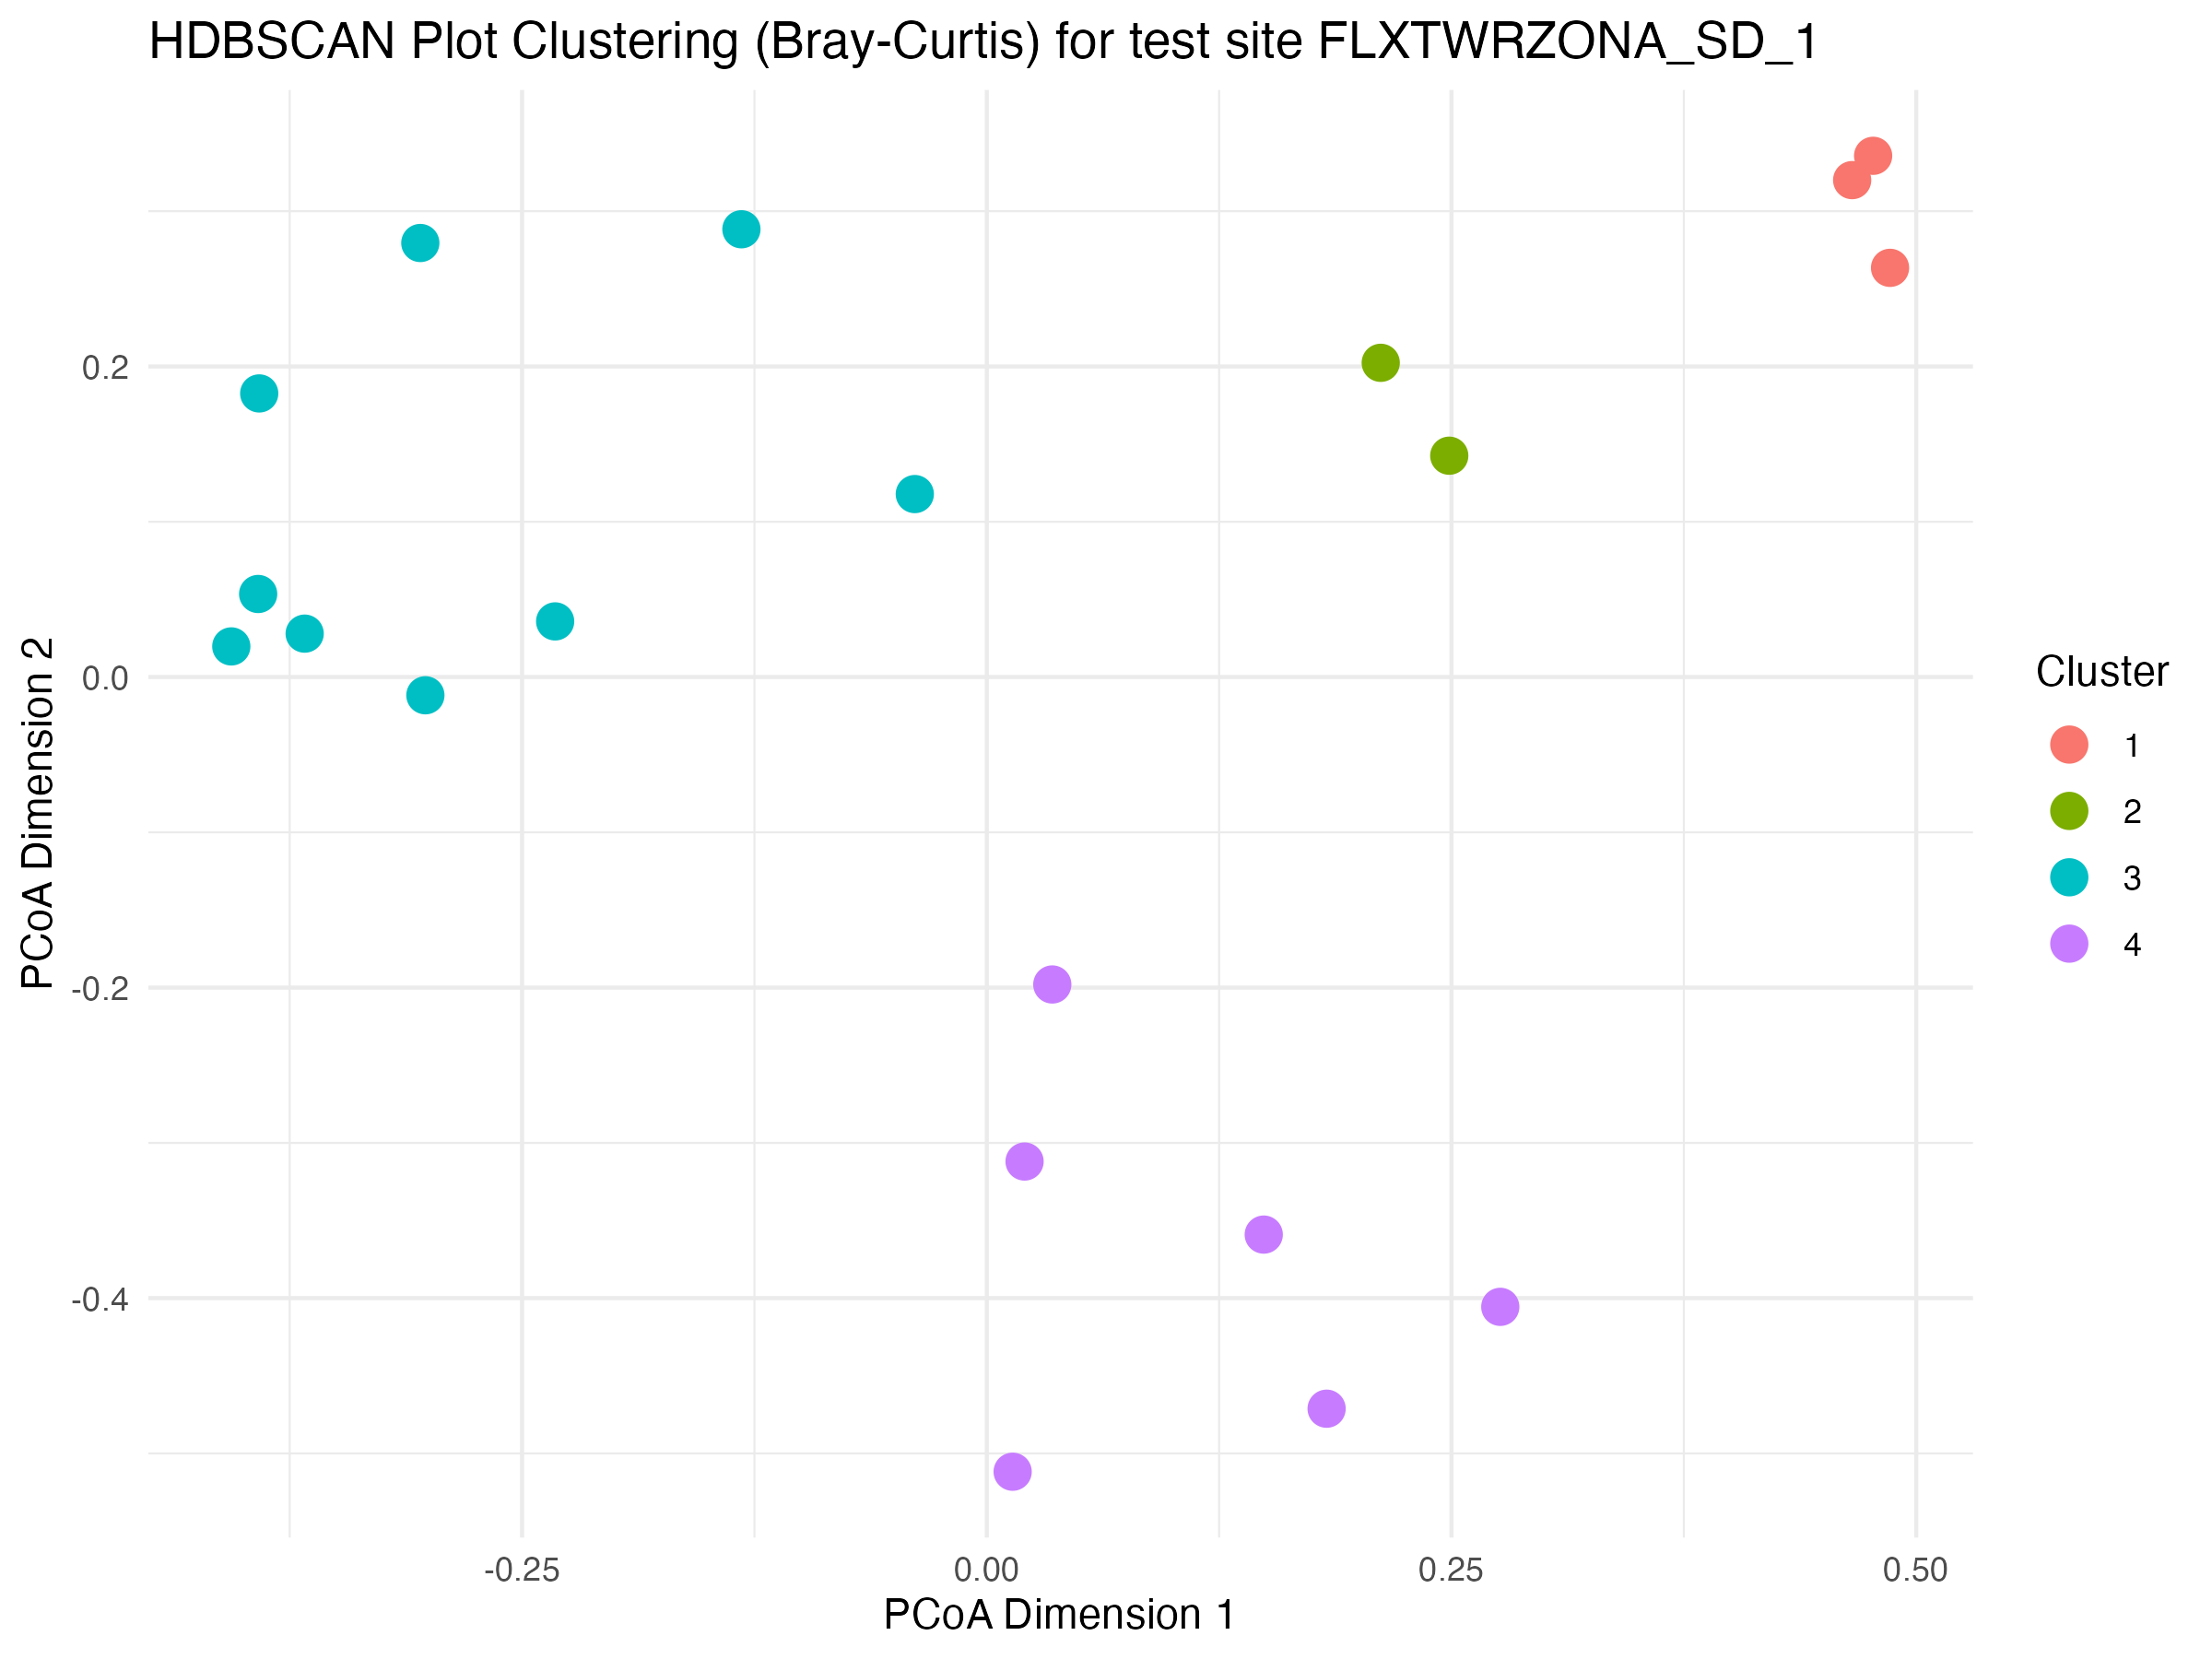
\includegraphics[width=\textwidth]{Figures/Appendix/PlantCommunityClustering/FLXTWRZONA_SD_1_HDBSCAN_clusters.png}
%         \caption{FLXTWRZONA\_SD\_1}
%         \label{fig:FLXTWRZONA_SD_1_HDBSCAN_clusters}
%     \end{minipage}
%     \hfill
%     \begin{minipage}[b]{0.45\textwidth}
%         \centering
%         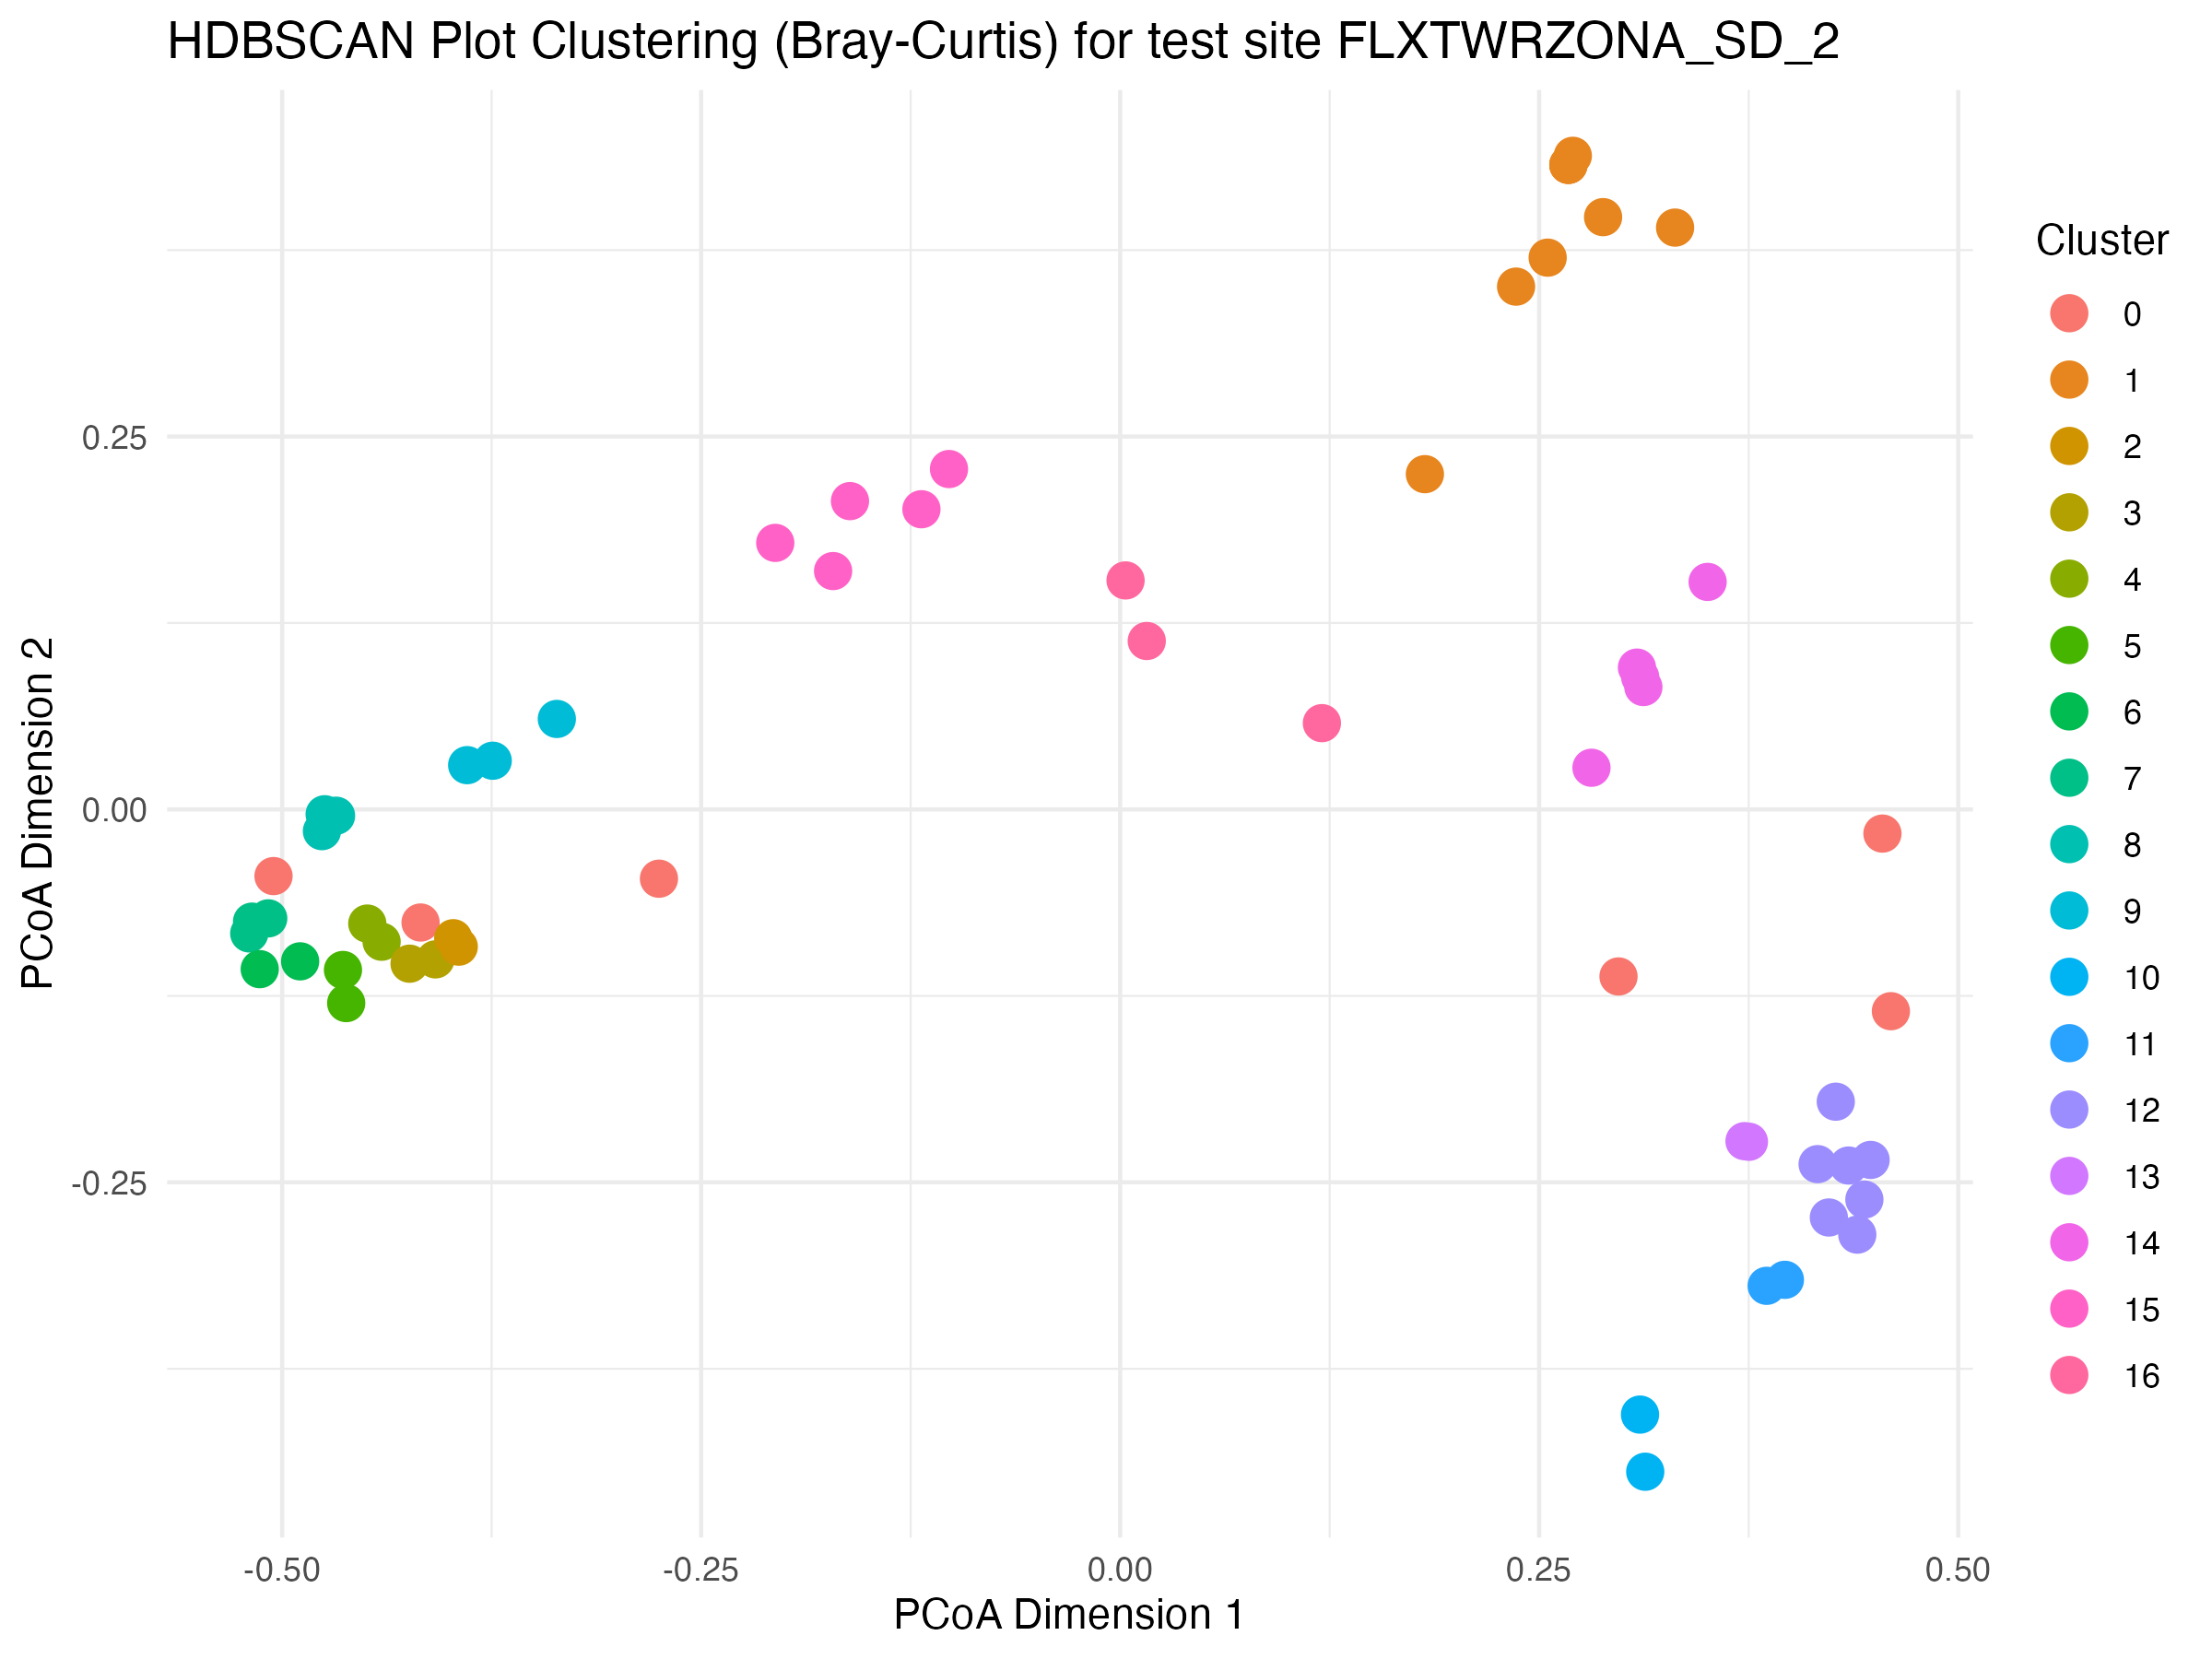
\includegraphics[width=\textwidth]{Figures/Appendix/PlantCommunityClustering/FLXTWRZONA_SD_2_HDBSCAN_clusters.png}
%         \caption{FLXTWRZONA\_SD\_2}
%         \label{fig:FLXTWRZONA_SD_2_HDBSCAN_clusters}
%     \end{minipage}

%     \vspace{1cm} % Space between rows of images

%     \begin{minipage}[b]{0.45\textwidth}
%         \centering
%         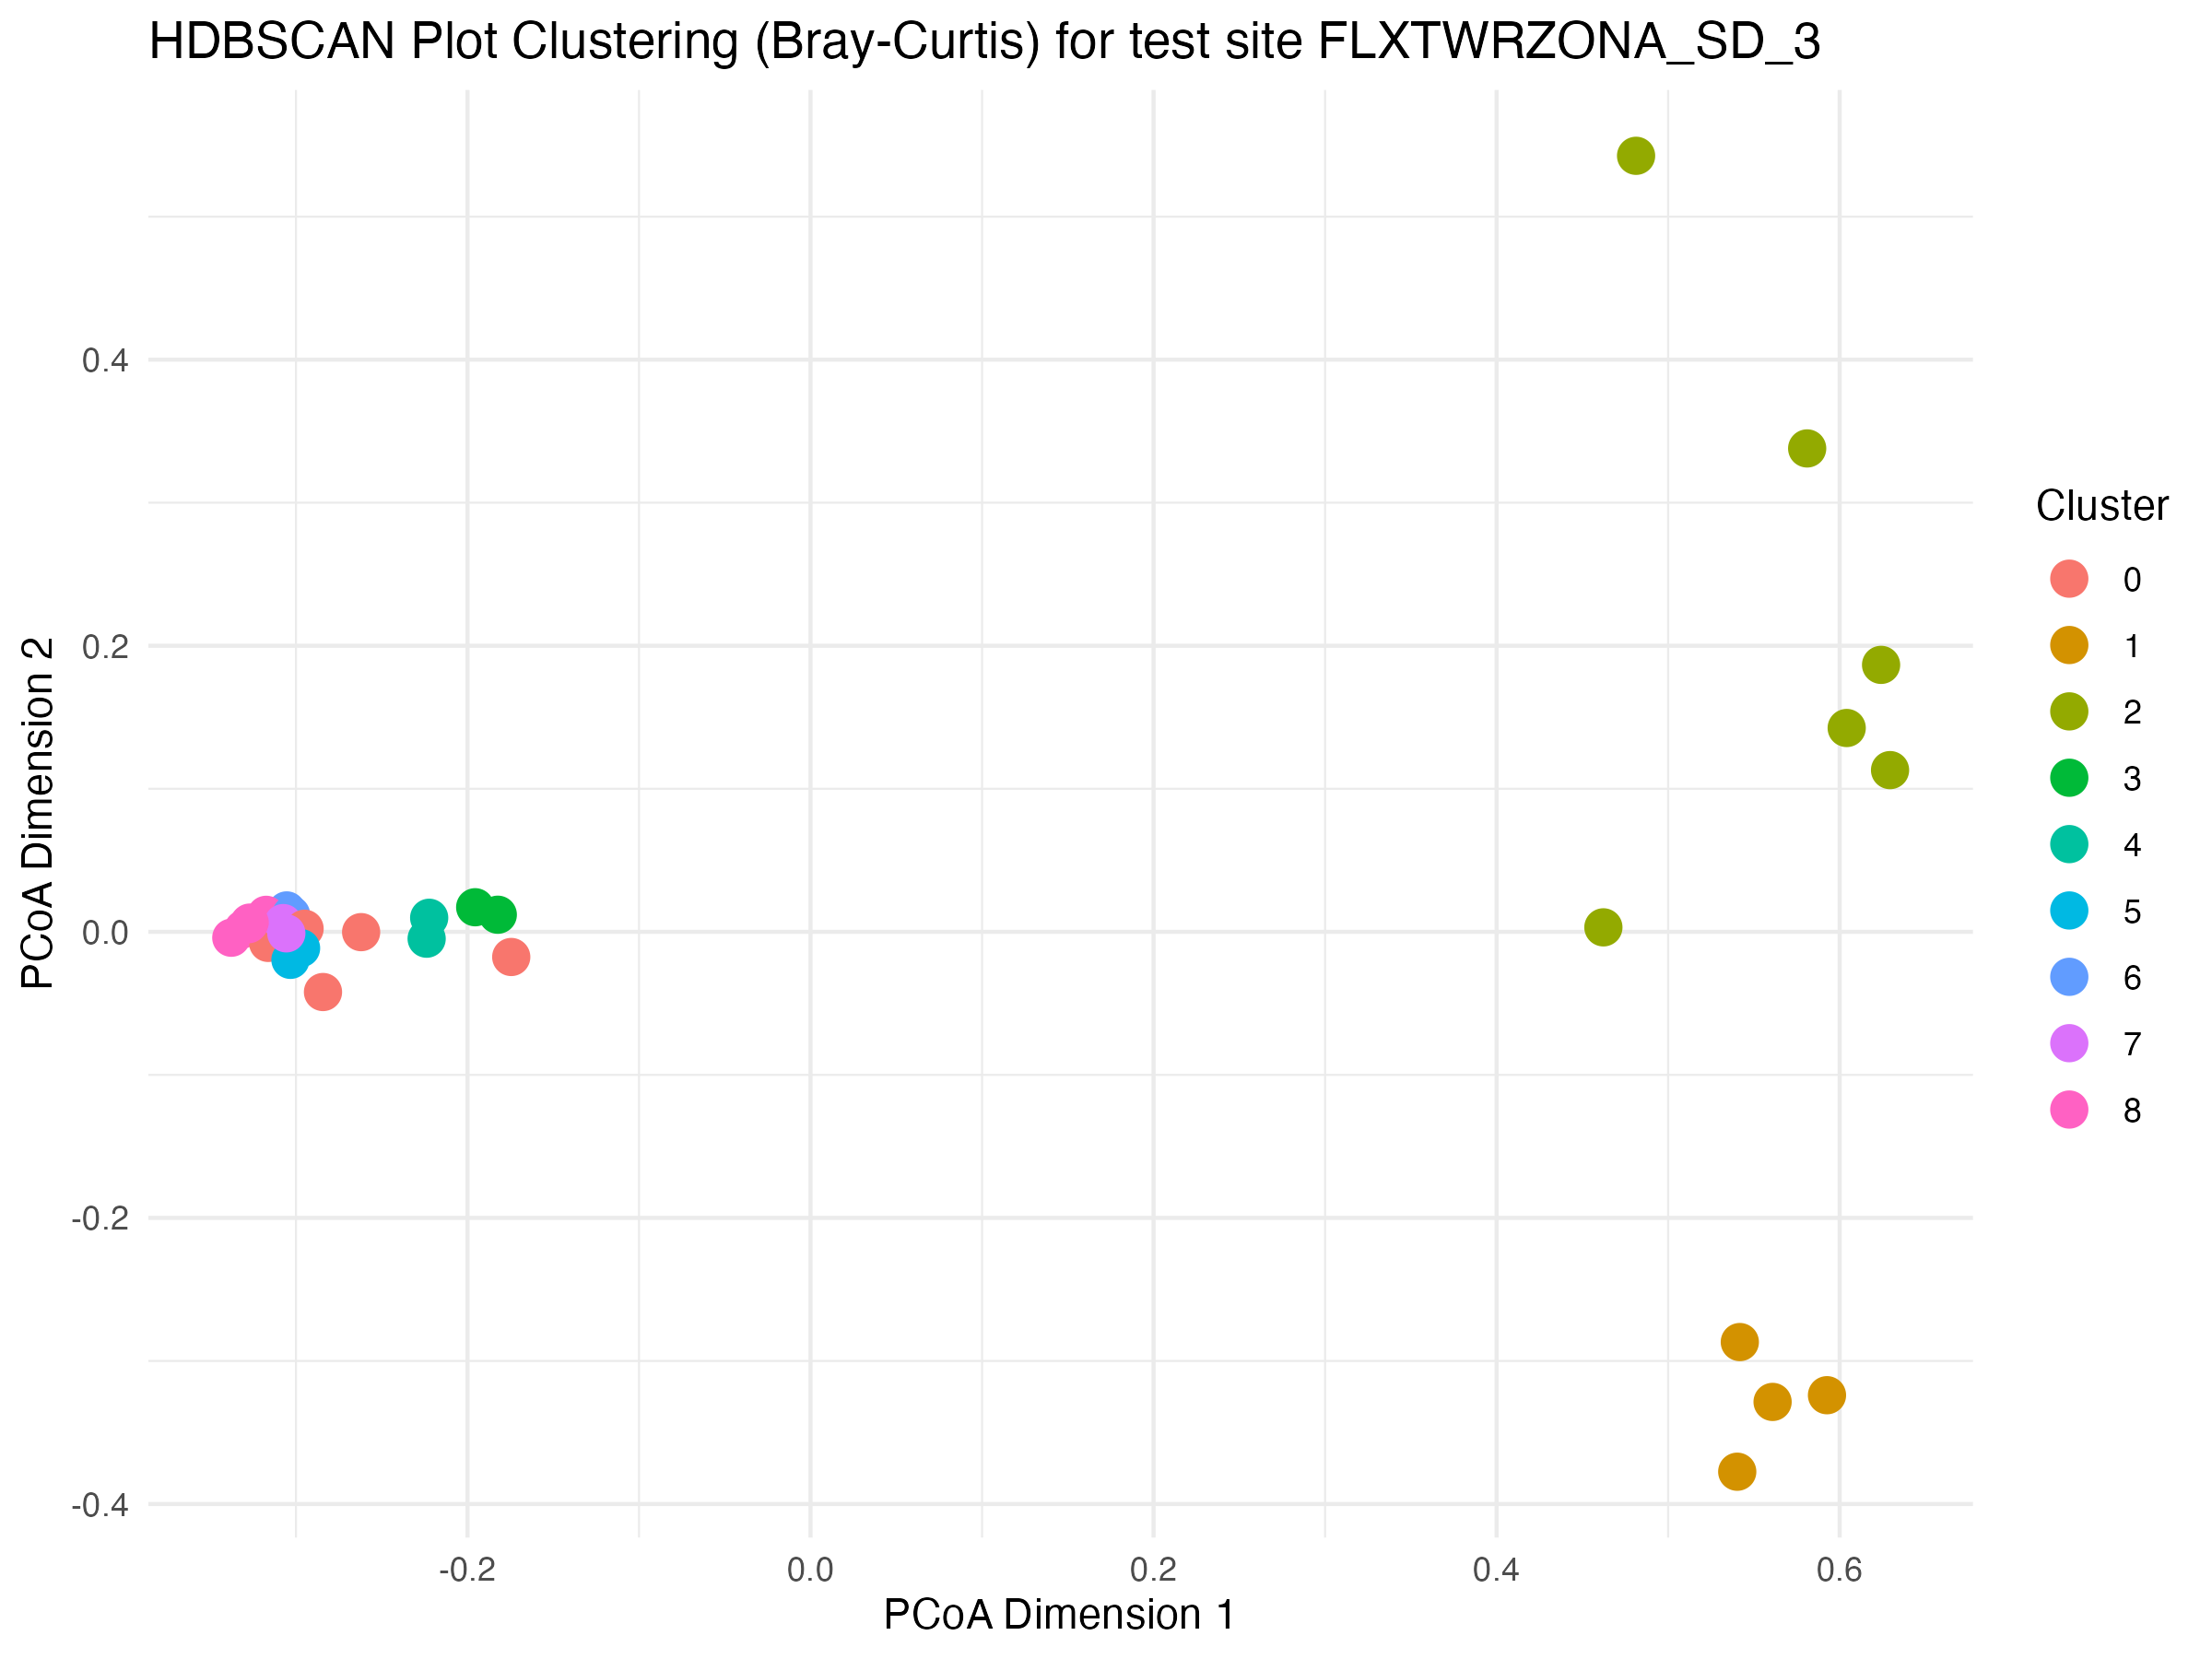
\includegraphics[width=\textwidth]{Figures/Appendix/PlantCommunityClustering/FLXTWRZONA_SD_3_HDBSCAN_clusters.png}
%         \caption{FLXTWRZONA\_SD\_3}
%         \label{fig:FLXTWRZONA_SD_3_HDBSCAN_clusters}
%     \end{minipage}
%     \hfill
%     \begin{minipage}[b]{0.45\textwidth}
%         \centering
%         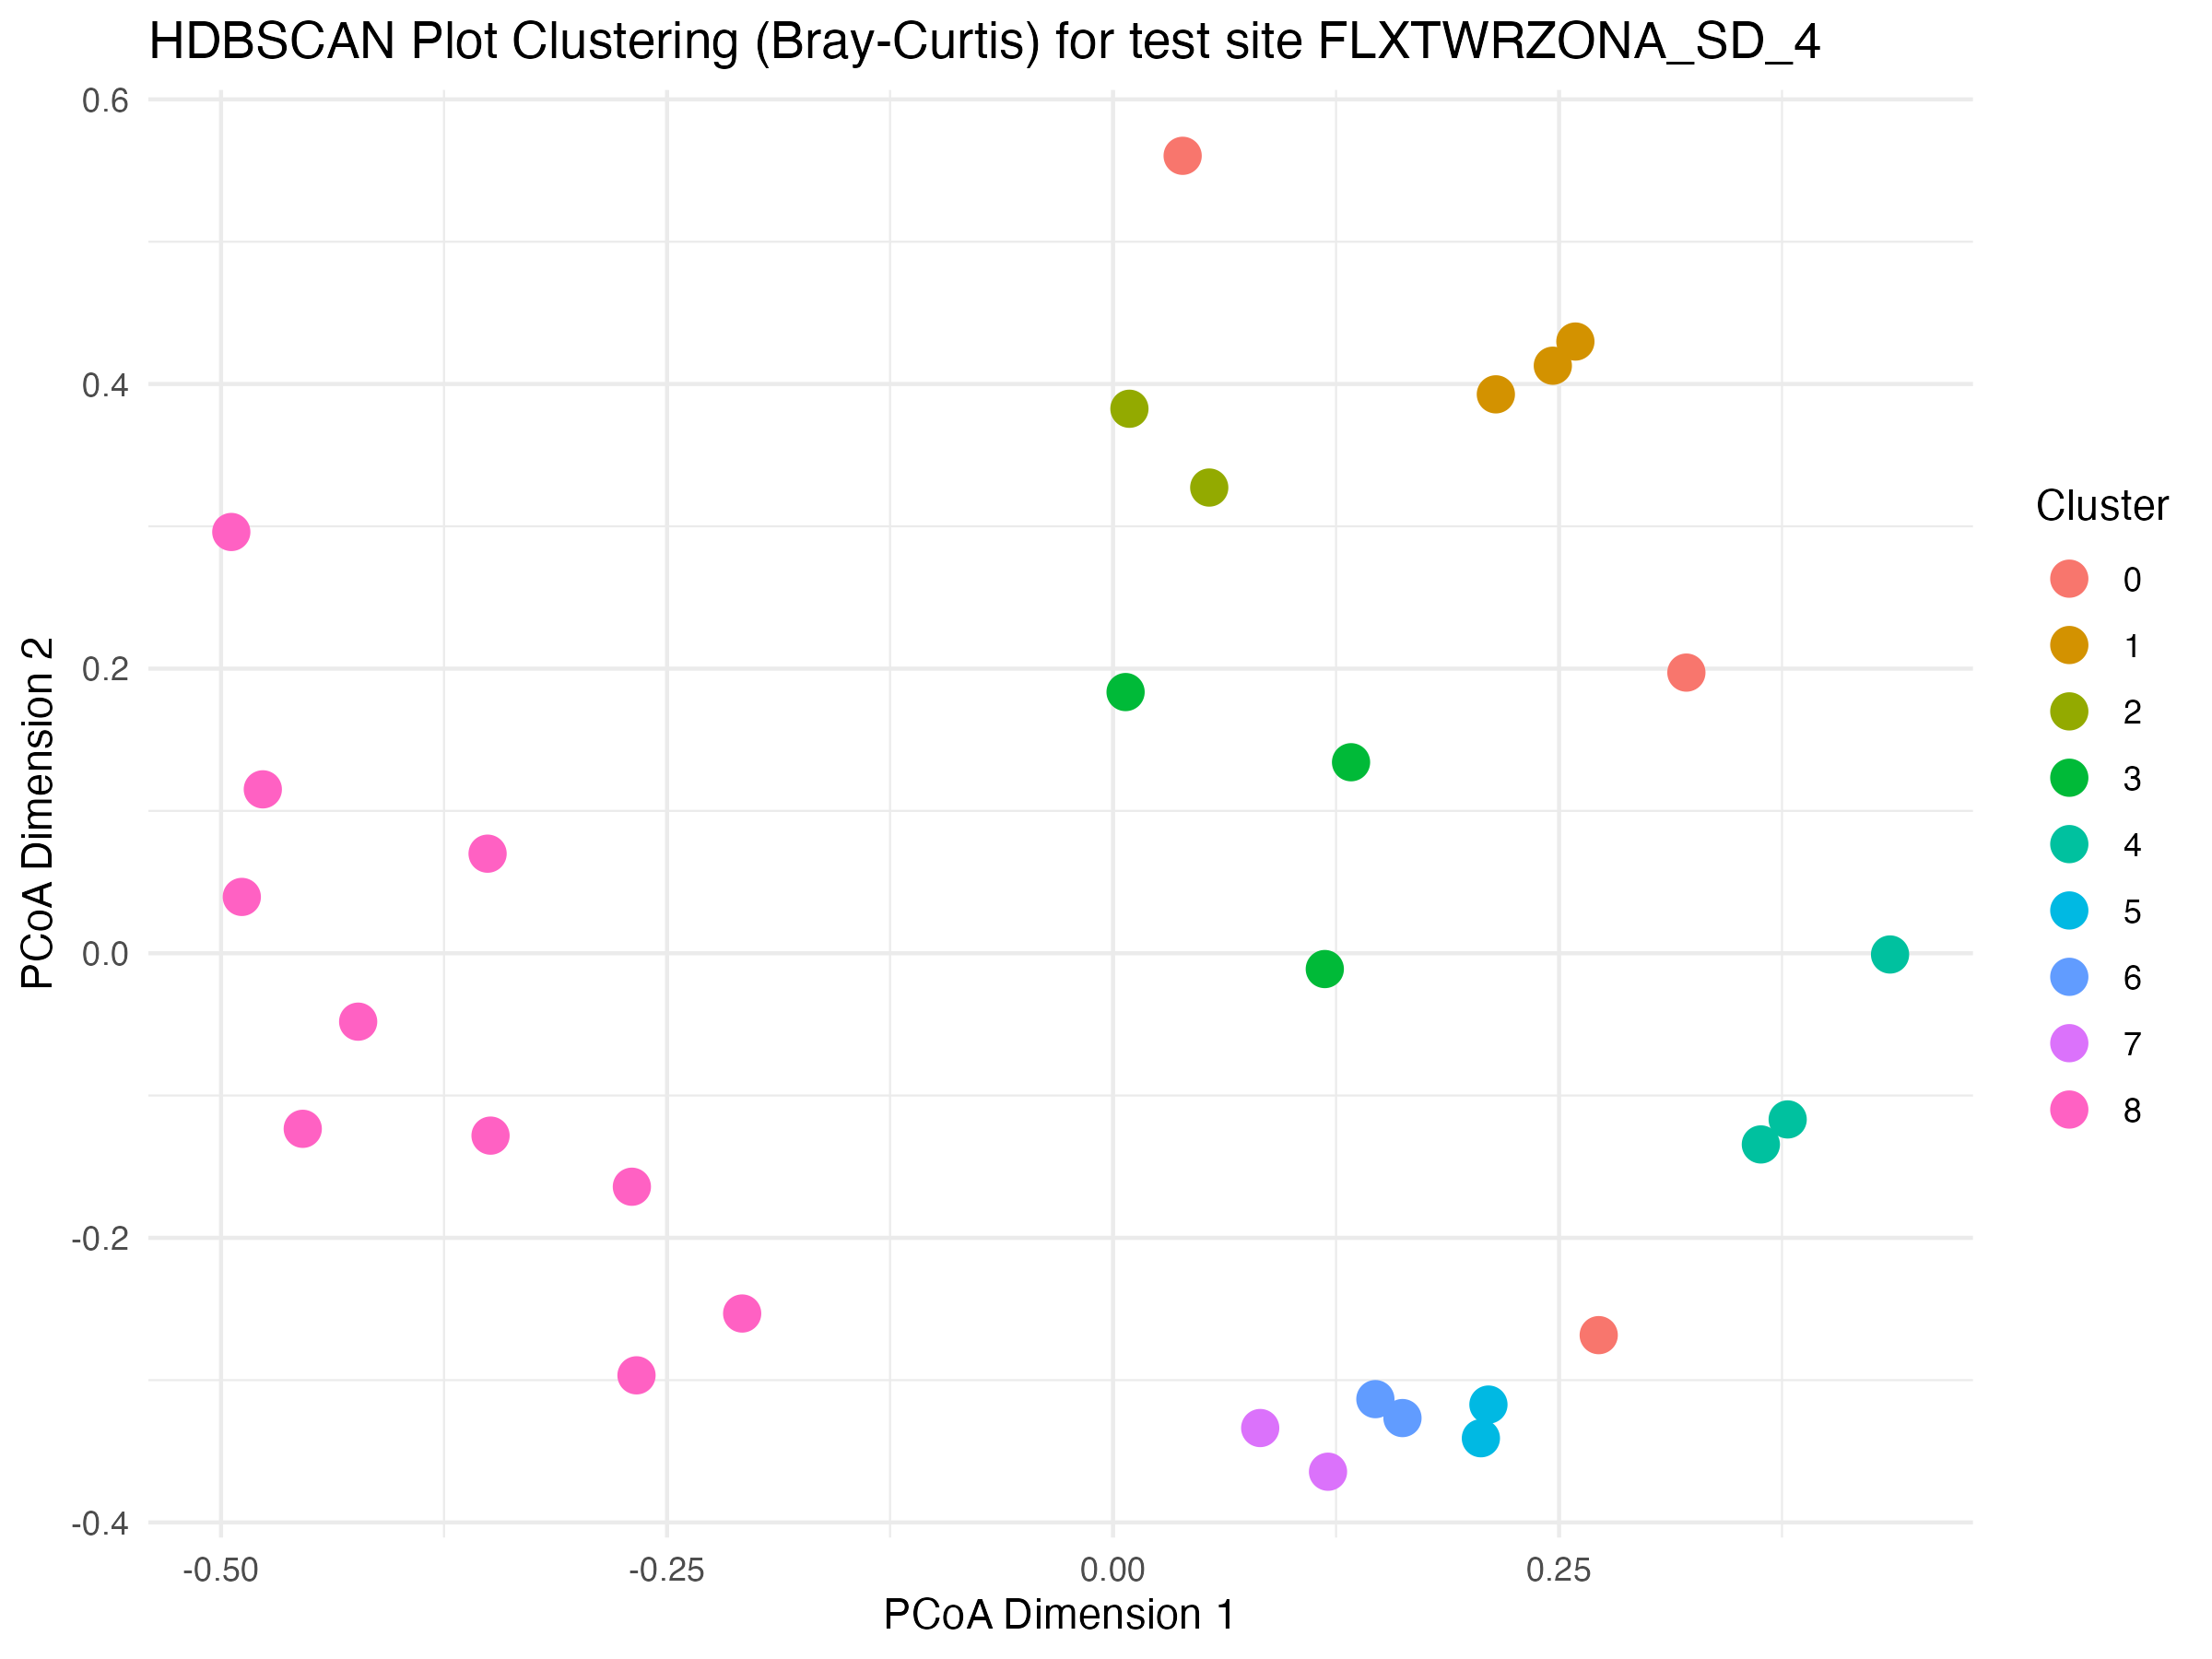
\includegraphics[width=\textwidth]{Figures/Appendix/PlantCommunityClustering/FLXTWRZONA_SD_4_HDBSCAN_clusters.png}
%         \caption{FLXTWRZONA\_SD\_4}
%         \label{fig:FLXTWRZONA_SD_4_HDBSCAN_clusters}
%     \end{minipage}
%     \captionof{figure}{Community Cluster Plots for Test Sites FLXTWRZONA\_SD\_1, FLXTWRZONA\_SD\_2, FLXTWRZONA\_SD\_3, and FLXTWRZONA\_SD\_4}
%     \label{fig:group2_clusters}
% \end{figure}

% % Group 3 of 4 (remaining plots)
% \begin{figure}[H]
%     \centering
%     \begin{minipage}[b]{0.45\textwidth}
%         \centering
%         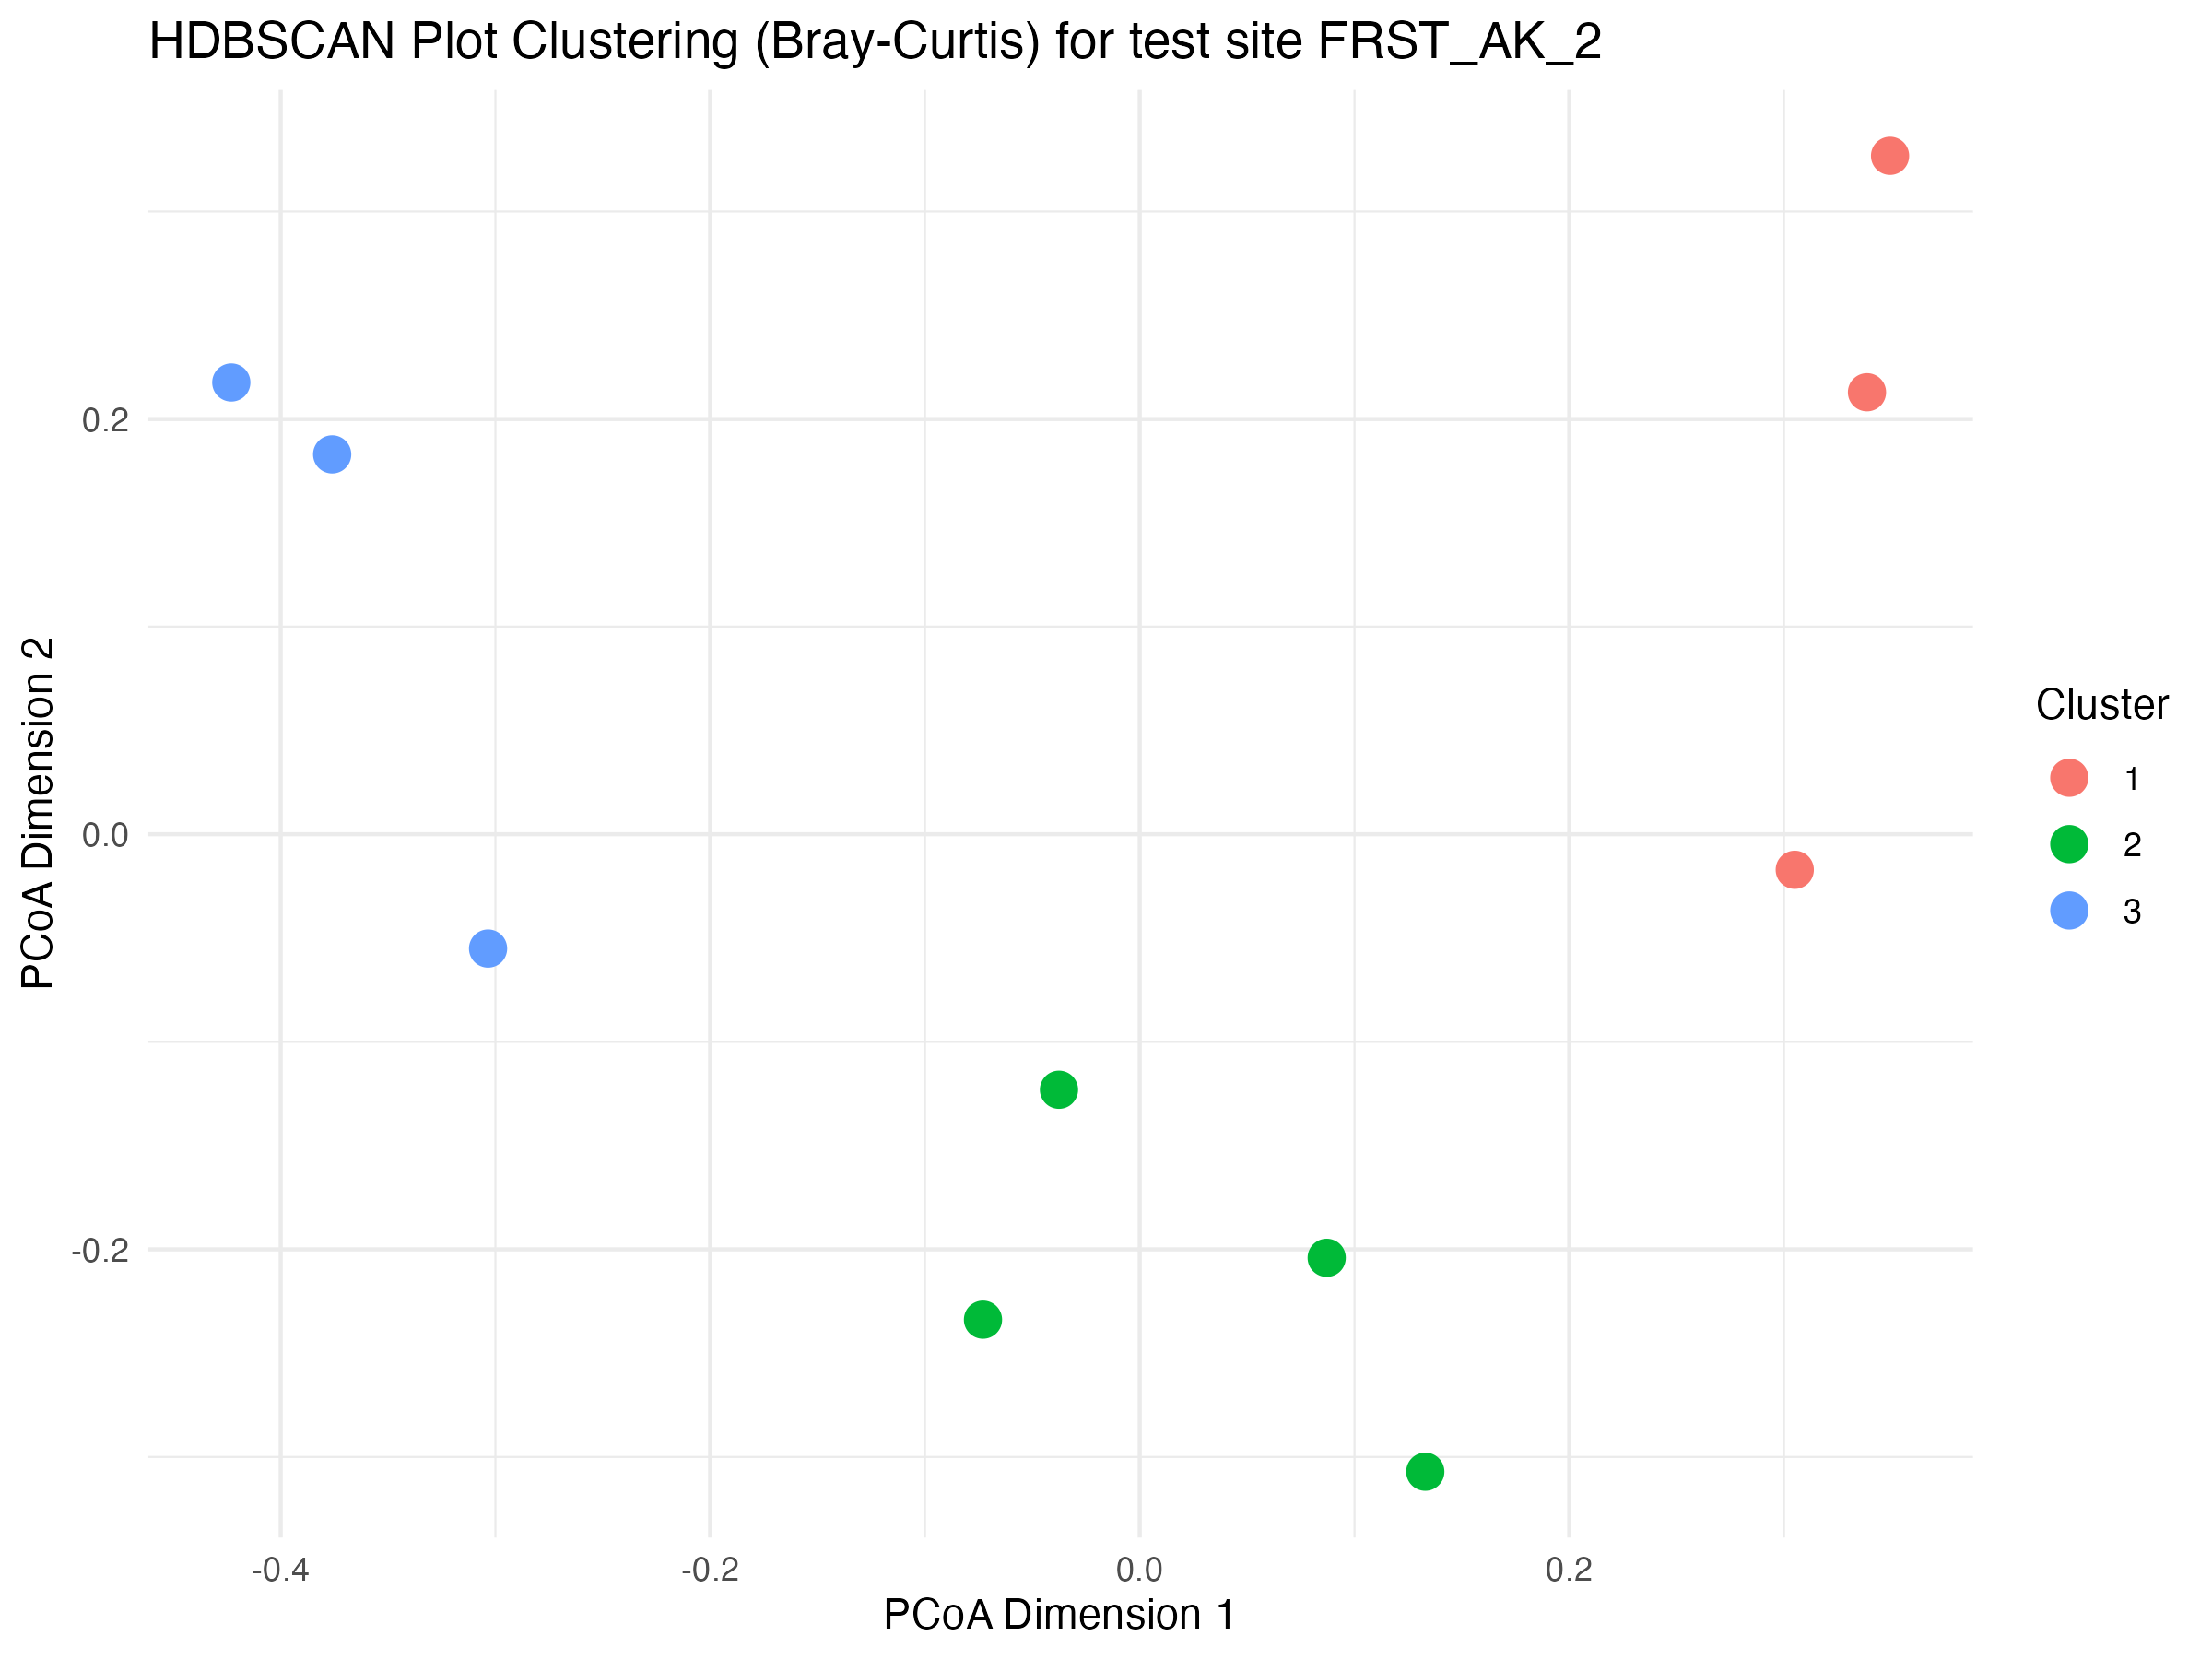
\includegraphics[width=\textwidth]{Figures/Appendix/PlantCommunityClustering/FRST_AK_2_HDBSCAN_clusters.png}
%         \caption{FRST\_AK\_2}
%         \label{fig:FRST_AK_2_HDBSCAN_clusters}
%     \end{minipage}
%     \hfill
%     \begin{minipage}[b]{0.45\textwidth}
%         \centering
%         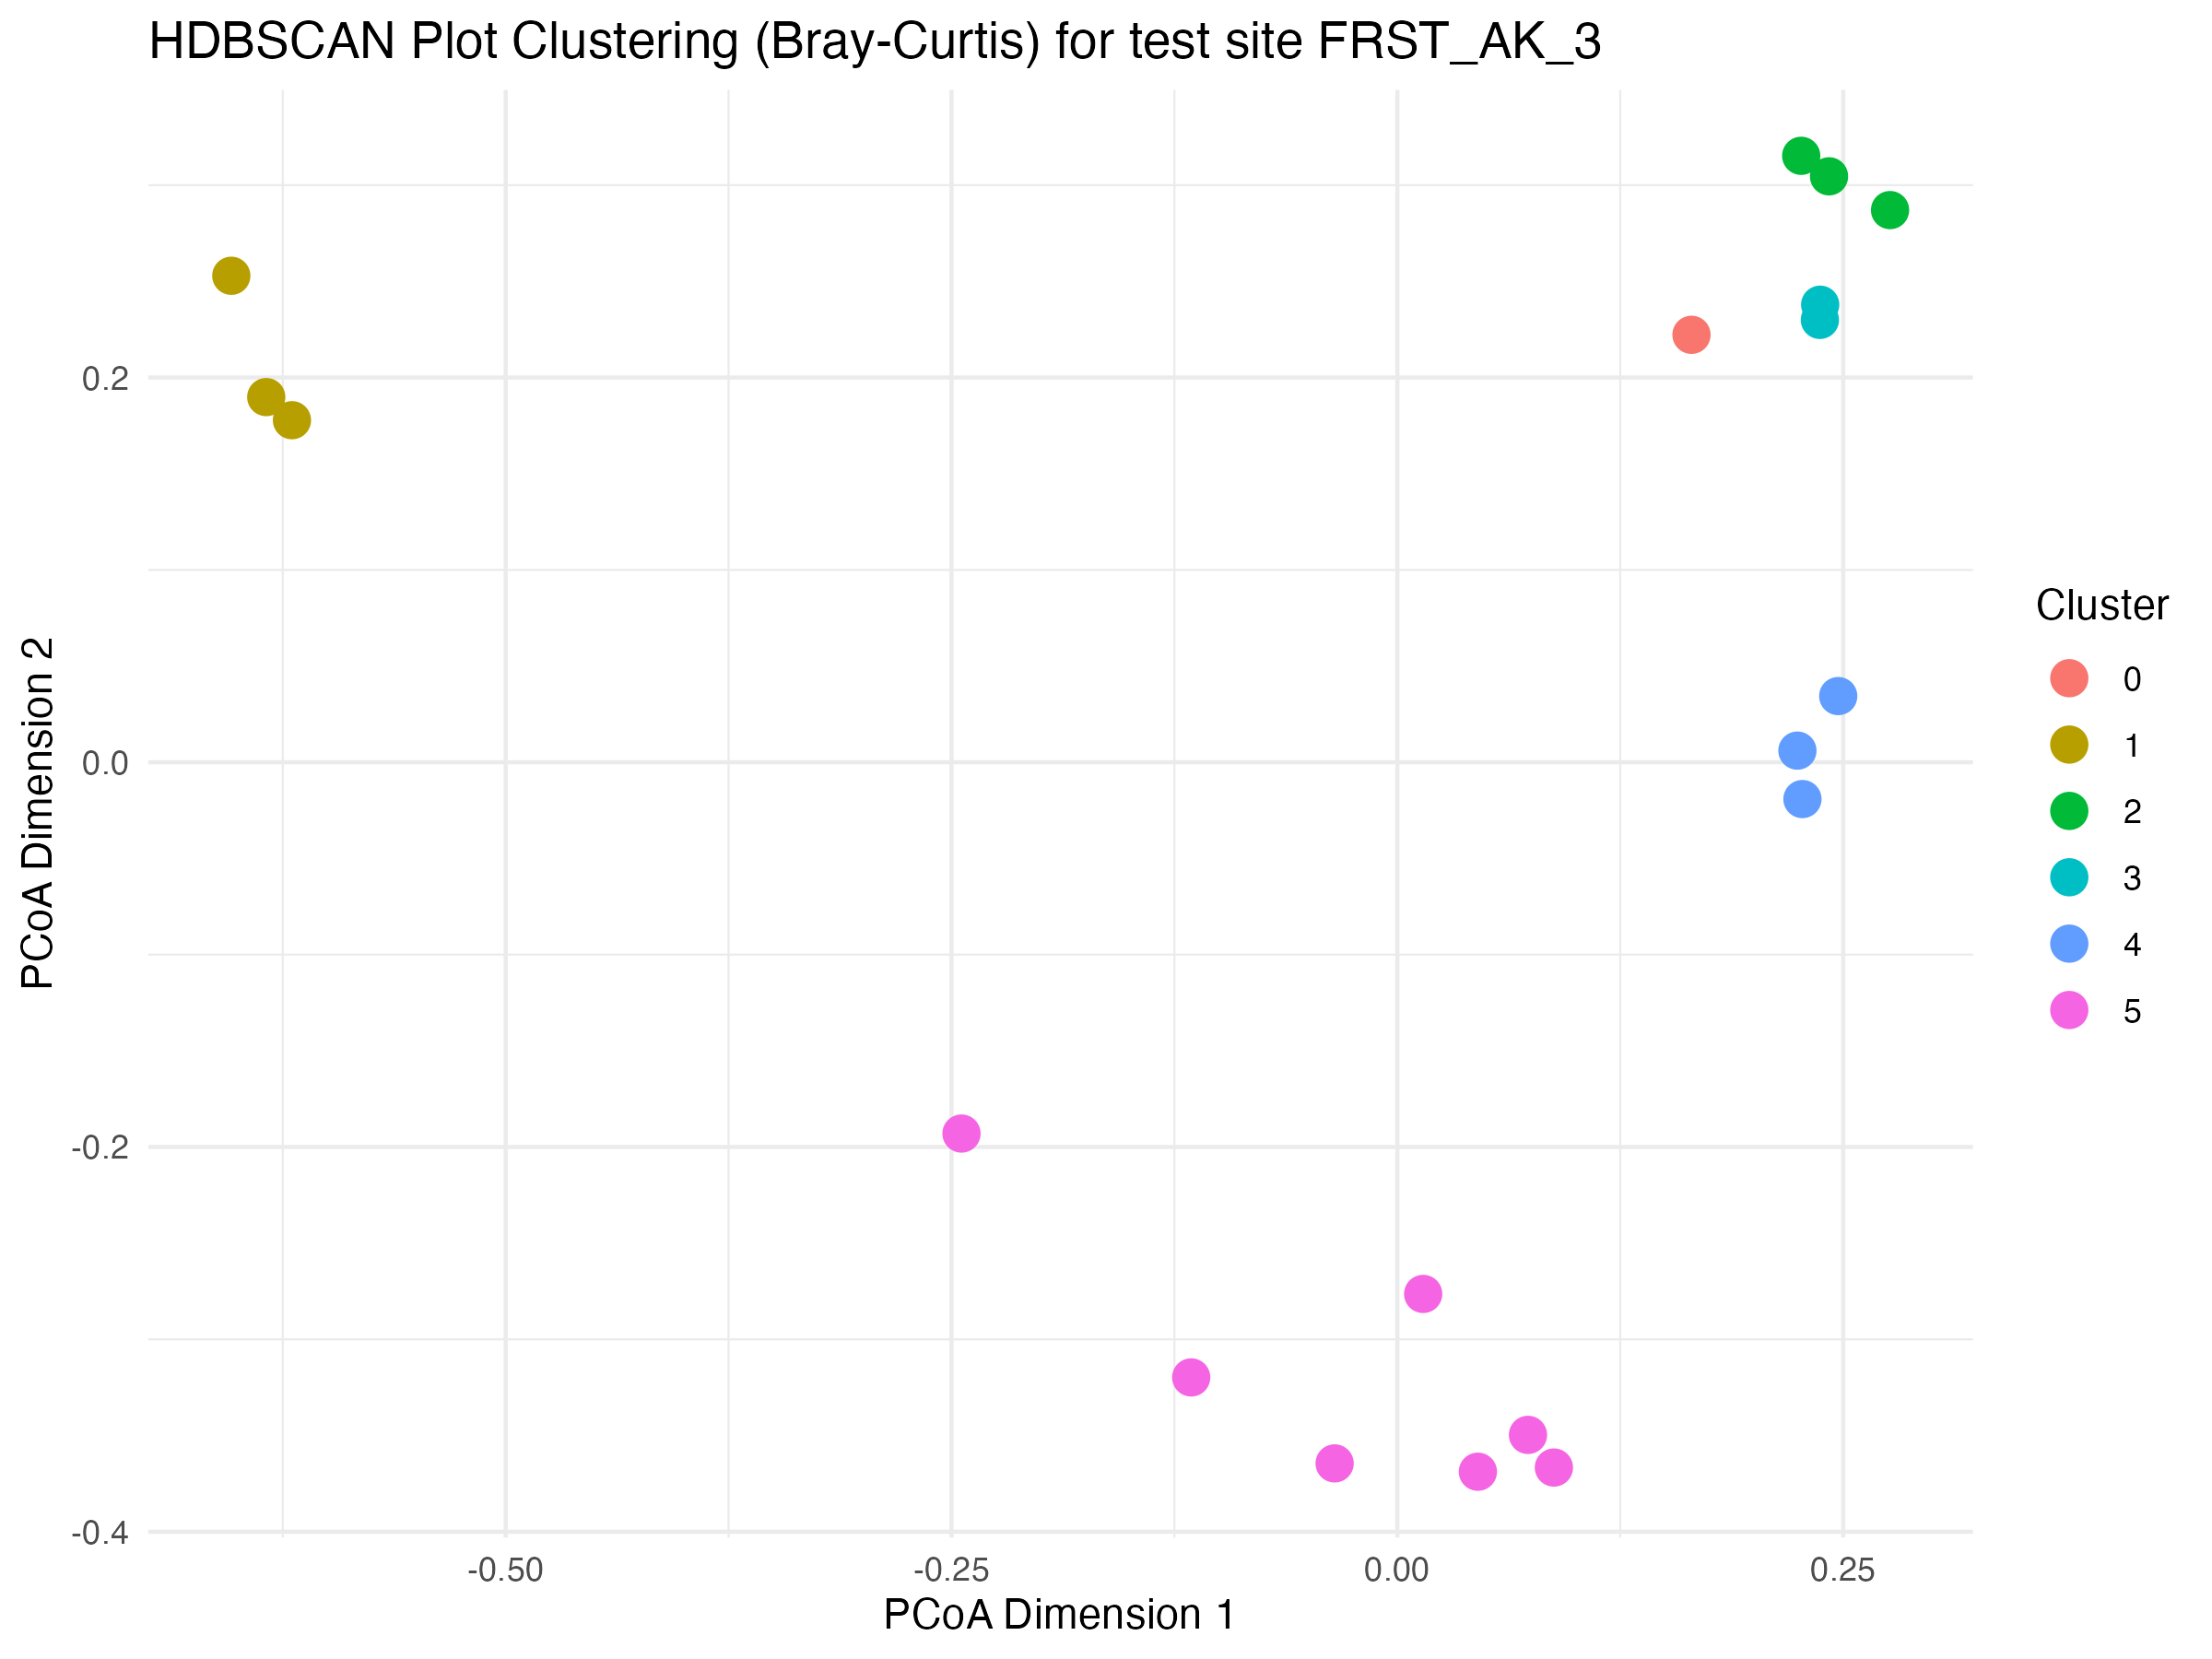
\includegraphics[width=\textwidth]{Figures/Appendix/PlantCommunityClustering/FRST_AK_3_HDBSCAN_clusters.png}
%         \caption{FRST\_AK\_3}
%         \label{fig:FRST_AK_3_HDBSCAN_clusters}
%     \end{minipage}

%     \vspace{1cm} % Space between rows of images

%     \begin{minipage}[b]{0.45\textwidth}
%         \centering
%         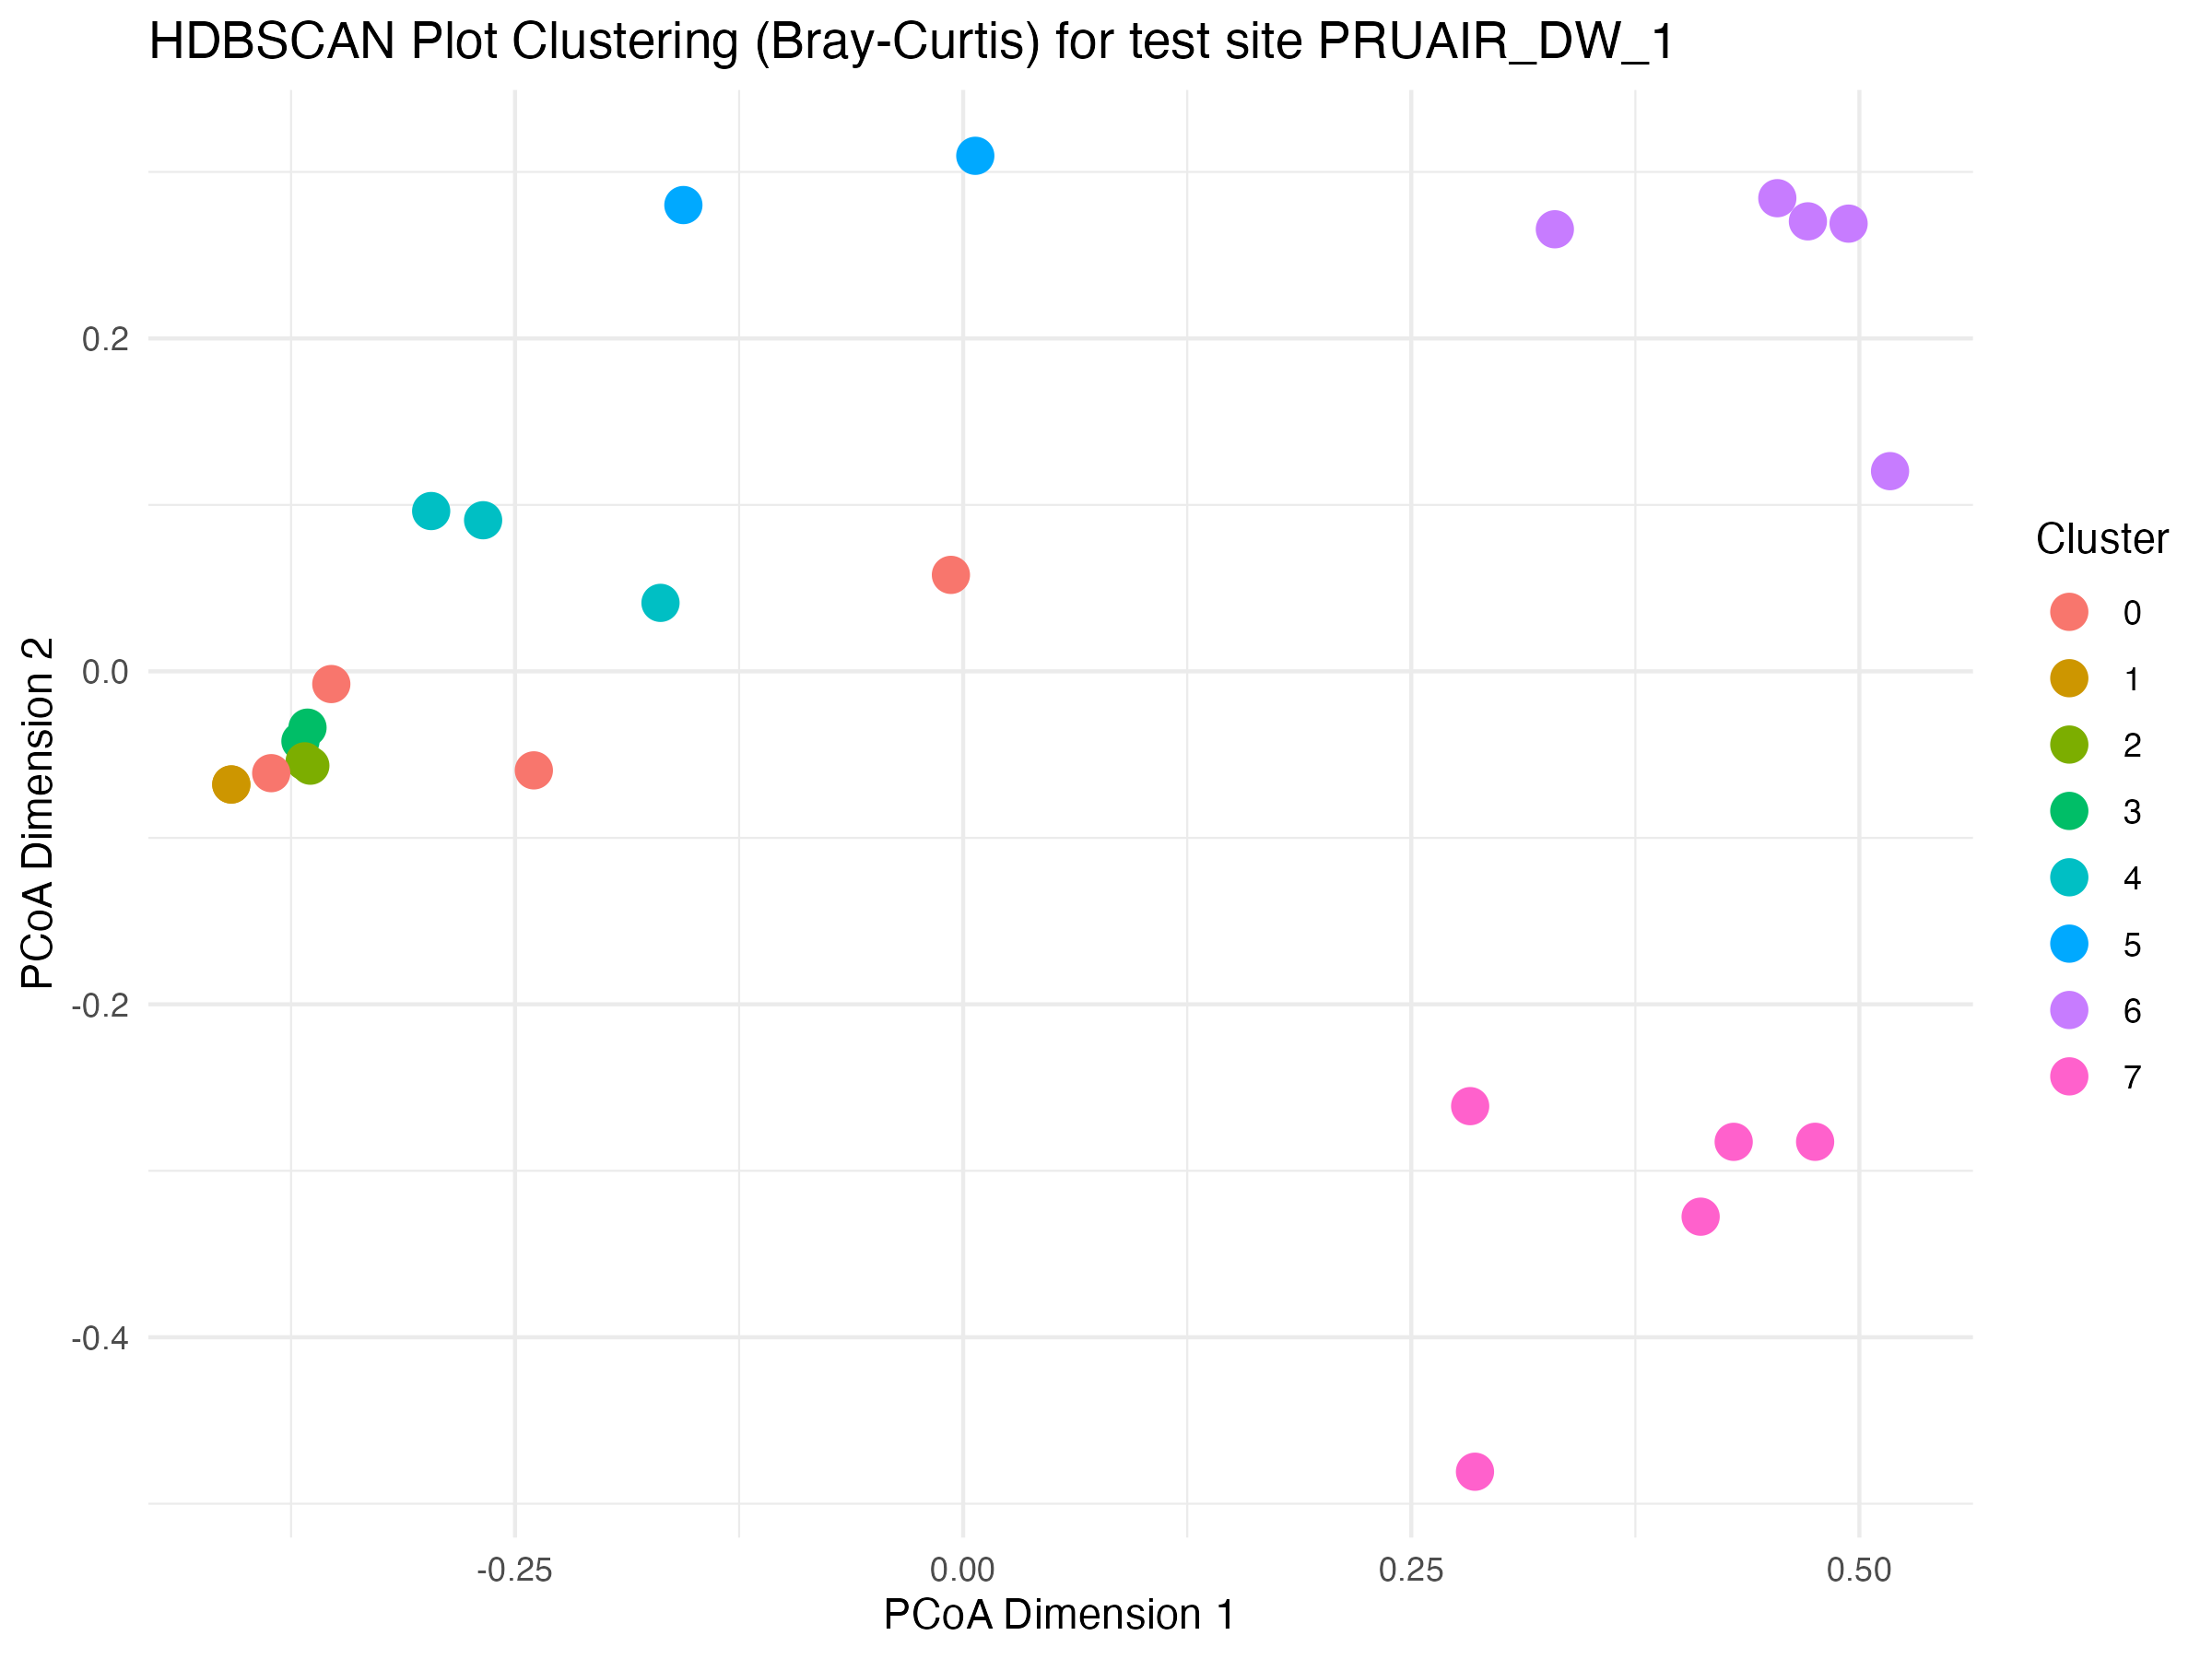
\includegraphics[width=\textwidth]{Figures/Appendix/PlantCommunityClustering/PRUAIR_DW_1_HDBSCAN_clusters.png}
%         \caption{PRUAIR\_DW\_1}
%         \label{fig:PRUAIR_DW_1_HDBSCAN_clusters}
%     \end{minipage}
%     \hfill
%     \begin{minipage}[b]{0.45\textwidth}
%         \centering
%         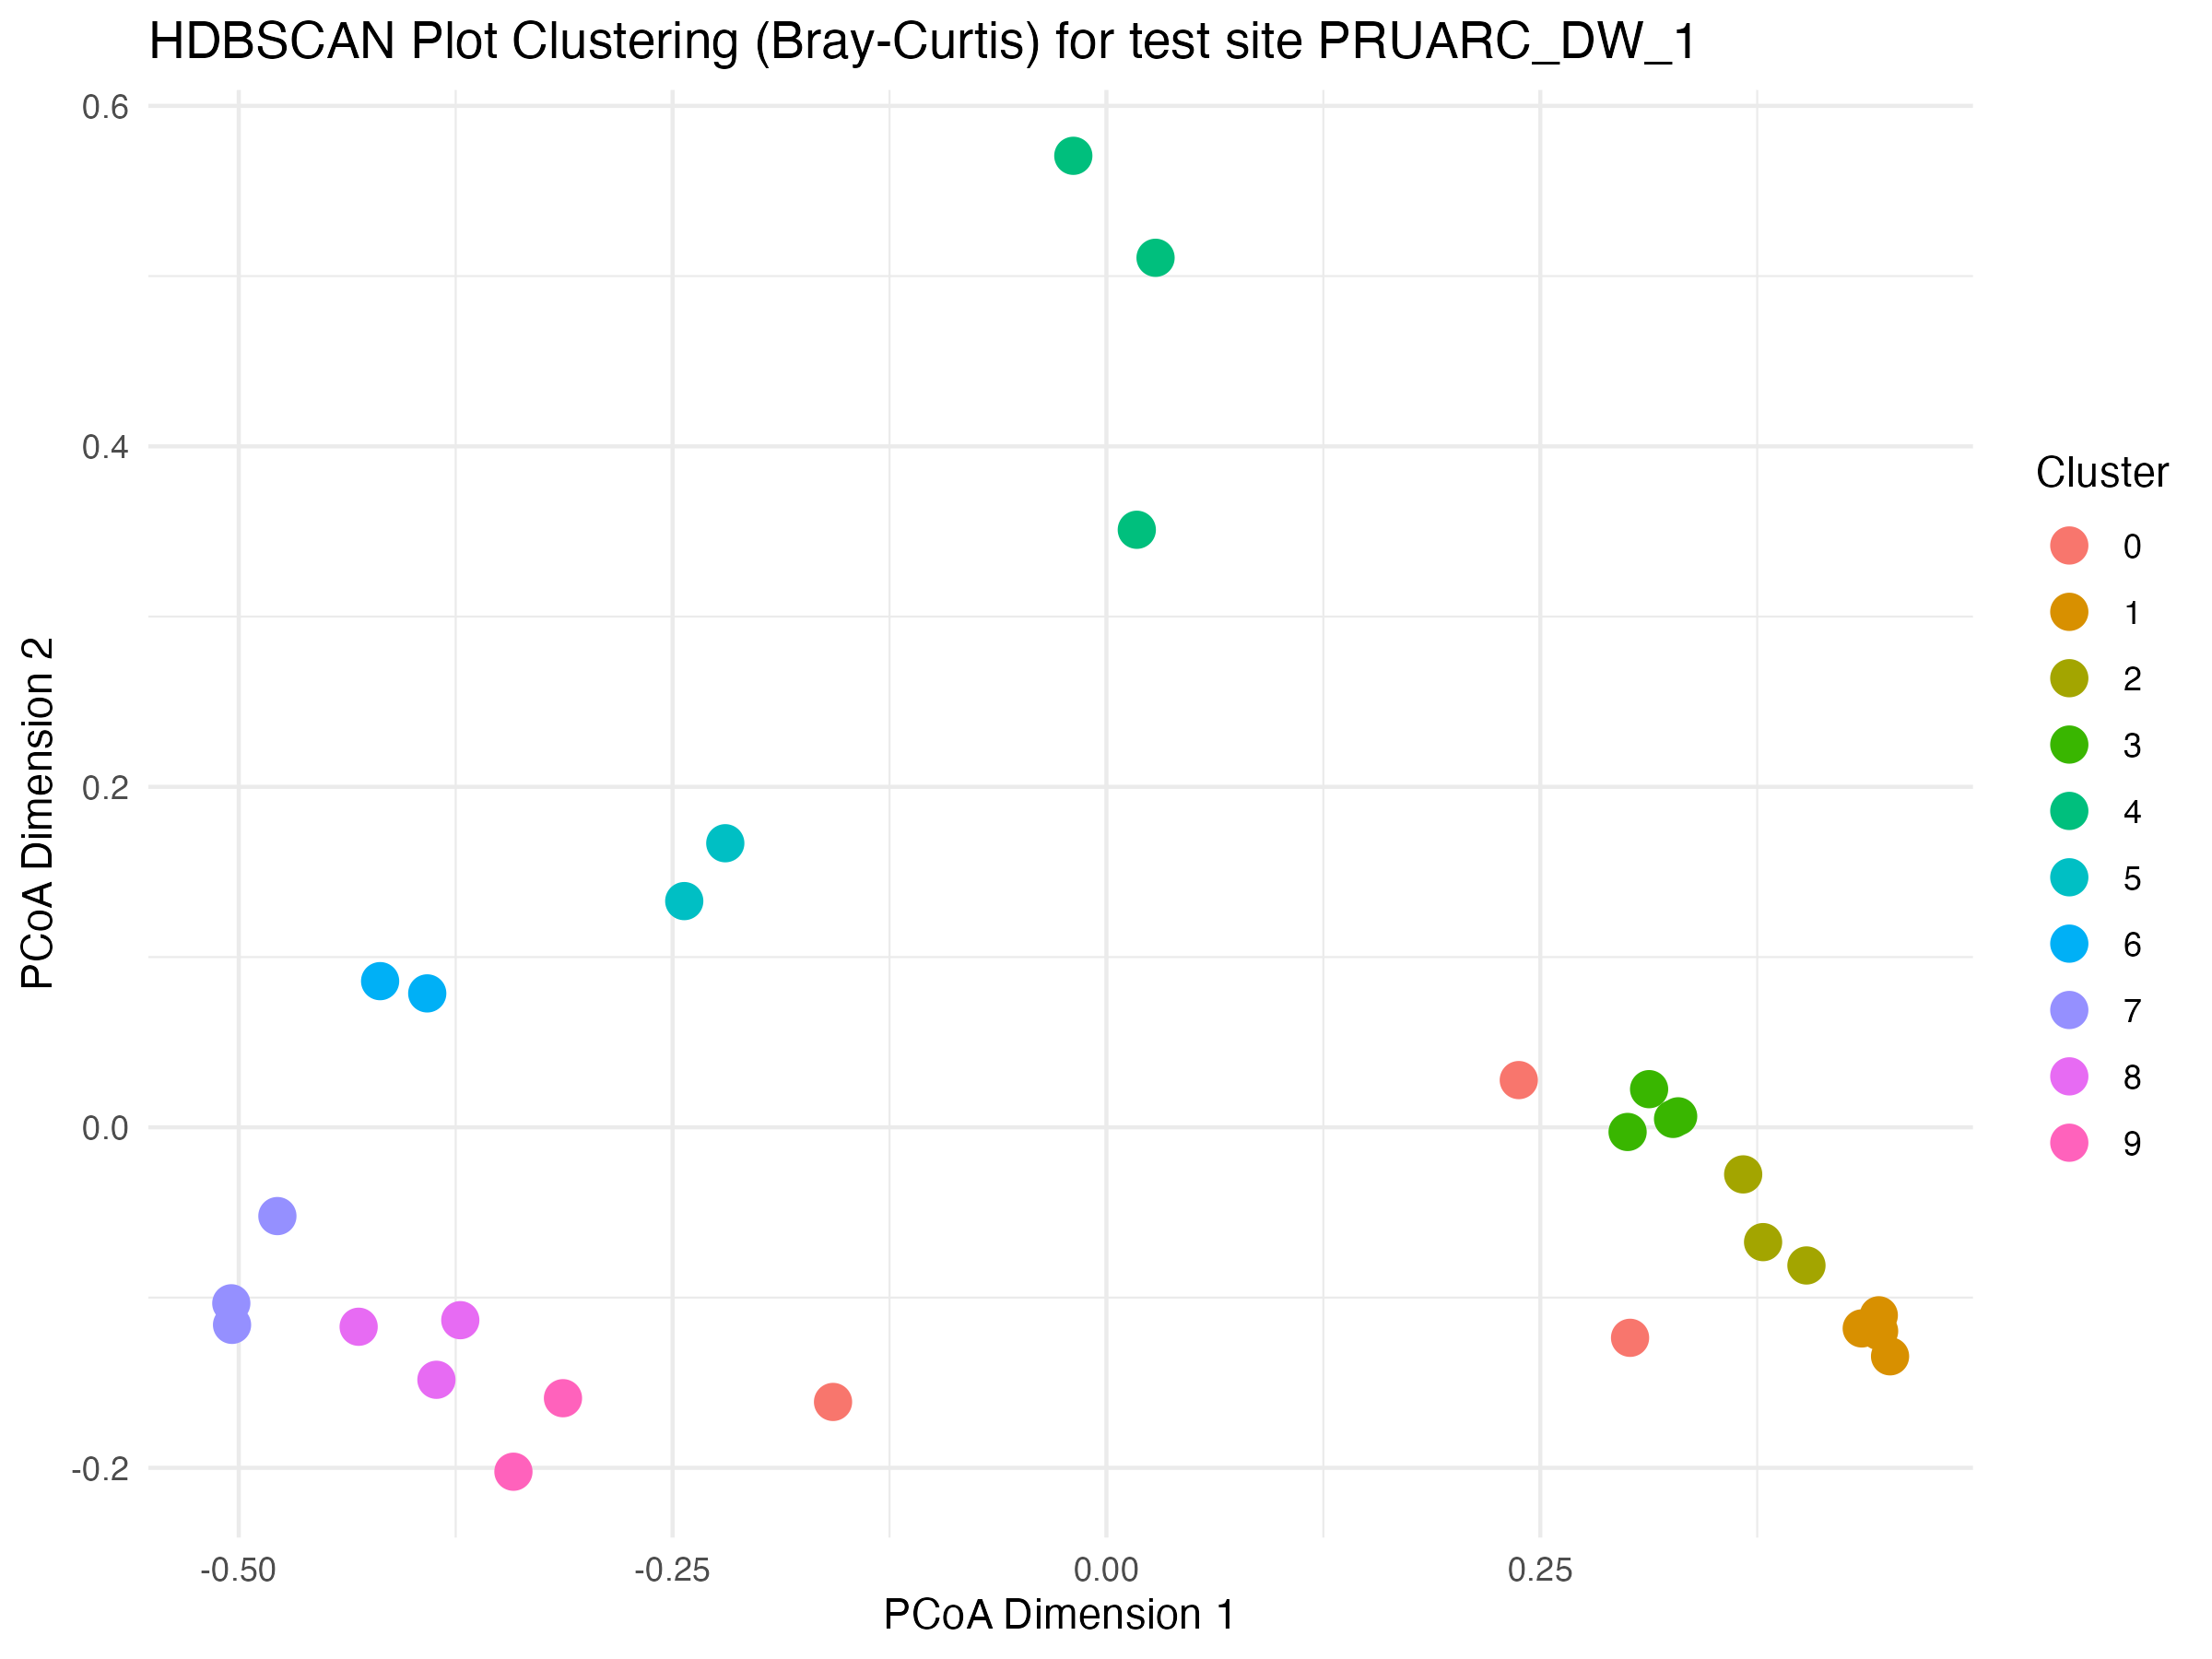
\includegraphics[width=\textwidth]{Figures/Appendix/PlantCommunityClustering/PRUARC_DW_1_HDBSCAN_clusters.png}
%         \caption{PRUARC\_DW\_1}
%         \label{fig:PRUARC_DW_1_HDBSCAN_clusters}
%     \end{minipage}
%     \captionof{figure}{Community Cluster Plots for Test Sites FRST\_AK\_2, FRST\_AK\_3, PRUAIR\_DW\_1, and PRUARC\_DW\_1}
%     \label{fig:group3_clusters}
% \end{figure}

%----------------------------------------------------------------------------------------
% BIBLIOGRAPHY
%----------------------------------------------------------------------------------------
\printbibliography[heading=bibintoc]


%----------------------------------------------------------------------------------------
\end{document}  
